\documentclass[10pt]{article}
\usepackage[a4paper,includeheadfoot,margin=2.54cm]{geometry}
\usepackage{booktabs}
\usepackage[square,numbers]{natbib}
\usepackage{graphicx}
\usepackage{amsmath}
\usepackage{mwe}
\usepackage{url}
\usepackage{comment}
\usepackage{verbatim}
\usepackage[pdftex]{hyperref}
\usepackage{adjustbox}
\usepackage{setspace}
\usepackage{caption}
\usepackage[list=true, hypcap=true]{subcaption}
\usepackage{paralist}
\usepackage{changepage}
\usepackage{pgfplots}
\pgfplotsset{compat=1.16}
\usepackage{float}
\usepackage{parskip}
\parskip=\baselineskip
\usepackage{gensymb}
\usepackage[T1]{fontenc}
\usepackage{xcolor}
\usepackage[notlot,nottoc,notlof]{tocbibind}

% Multiline URLs
\def\UrlBreaks{\do\/\do-}

\newcommand{\CS}{C\nolinebreak\hspace{-.05em}\raisebox{.6ex}{\scriptsize\bf \#}}
\onehalfspacing
\graphicspath{ {./images/} }
\newenvironment{container}{}

% Create subsubsubsection, and add to section count (and ToC if required)
\newcommand{\subsubsubsection}[1]{\paragraph{#1}\mbox{}\\}
\setcounter{secnumdepth}{4}

% Additional maths commands
\newcommand{\norm}[1]{\left\lVert #1 \right\rVert}
\renewcommand{\vec}[1]{\mathbf{#1}}
\newcommand*\mean[1]{\overline{#1}}

\begin{document}
\begin{titlepage}

\begin{minipage}{0.5\textwidth}
    \begin{flushleft}
    
\includegraphics[width=65mm]{images/University_of_Bristol_logo.png}
    \end{flushleft}
\end{minipage}
\begin{minipage}{0.5\textwidth}
    \begin{flushright}
    
\includegraphics[width=30mm]{images/Eng_Des_Logo.png}
    \end{flushright}
\end{minipage}

\centering
\vspace*{1.3\baselineskip}

\huge{Faculty of Engineering\\}
\vspace*{0.5\baselineskip}
\huge{BEng in Engineering Design\\}
\vspace*{0.75\baselineskip}

\LARGE{YEAR 4 PROJECT}

\vspace*{\baselineskip}

\LARGE{\textbf{Investigating Computer Vision for \\Production Line Health Estimation
}}
\vspace{1.3\baselineskip}

{\LARGE \textbf{Daniel Rodrigues}}\\

\vspace{1.3\baselineskip}

{\Large{Project thesis submitted in support of the degree of
\\Bachelor of Engineering\\
}}
\vspace{0.75\baselineskip}
{\large{Project Advisor: Jeff Barrie, Department of Civil Engineering
}}

\vspace{0.75\baselineskip}
\large{May 2021}

\end{titlepage}

\clearpage
\pagenumbering{roman}
\begin{container}
\section*{Acknowledgements}
I would like to thank Stephen Gilmore, Tim Quigg, Leo Green, and Nikita Alexander from Crux Product Design for supporting this project with their time and expertise, and for providing valuable insight into industry trends and regulations. At the University of Bristol, I would like to thank Jeff Barrie, for attempting to supervise the project in as turbulent a time as the present. I would also like to thank Paul Harper for his assistance across the year, both technical and pastoral, as well as Mike McCann for his assistance with scoping the project from the outset. I am additionally thankful to my project team (Ollie Fogg, James Irvin, and Jake Hodges) for their sustained effort throughout the year, resulting in a supportive, productive and exciting project time span, even amidst external challenges. Further gratitude is extended to the Open Source community for the development of numerous tools and libraries that have been used throughout this project, and have been central to the modelling activity. This is also particularly extended to the team at GitHub, who have facilitated easy and robust version control which has consistently saved the project from an assortment of weird and wacky ``technical issues''.

\vspace{0.6cm}
\section*{Declaration}
\textit{The accompanying research project report entitled: ``Investigating Computer Vision for Production Line Health Estimation'' is submitted in the fourth year of study towards an application for the degree Bachelor of Engineering in Engineering Design at the University of Bristol. The report is based upon independent work by the candidate. All contributions from others have been acknowledged above. The views expressed within the report are those of the author and not of the University of Bristol.}

\vspace{0.6cm}
\noindent I hereby declare that the above statements are true.

\vspace{0.4cm} 
\noindent Signed (author):
\begin{figure}[h]
    \includegraphics[width=30mm]{images/Signature.png}
    \label{fig:sig}
\end{figure}\\
\noindent Full Name:\\
Daniel Anthony Rodrigues

\noindent Date:\\
28 May 2021
\end{container}

\clearpage

\section*{Executive Summary}
The medical industry demands a high volume and sterility of borosilicate glass vials, necessitating the use of carefully controlled production lines. The two key contributors to line stoppages are tipped vials (46.6\%) and crushed glass (15.6\%), which can reduce product quality and operational efficiency, leading to major cost penalties. Companies are increasingly looking to new solutions to assist root cause analysis and provide a greater insight into the cause of these failures. 

This body of work is part of a wider group project which aims to develop novel analytical processes to help improve performance monitoring and analysis. This specific report considers the development of an image processing pipeline for visual health estimation.

A literature review highlighted a industry-wide trend towards increasingly automated, flexible, and data-driven monitoring techniques, for which image processing techniques are becoming increasingly popular. Existing systems were found to be either too specific or high-level in approach, highlighting an opportunity for an intermediary modular solution to address this commercial demand. 

A lack of real-world data was identified and mitigated through the development of synthetic data generation utilities. Blender was used to create a virtual vial, which was subsequently transferred into Unity and assigned a pseudo-glass appearance to be used across the required environments. These consisted of a rendering environment for detector development, and a simulation environment for the development of the tracker and analysis layer. These tools proved to be highly effective in progressing the project in the absence of supporting data.

Several promising detection and tracking techniques were identified during the literature review, and were subsequently implemented and benchmarked to identify the best-performing methods. The optimal pair of techniques was shown to be the Scaled-YOLOv4 object detector and centroid tracker, demonstrating the greatest speed, accuracy and robustness when applied to the test data.

A custom analysis layer was developed to address the common failure modes,  comprising of a localised damage assessment procedure and a macroscopic toppling risk assessment process. Although uncalibrated, it demonstrated great potential for commercial applicability, providing rich insights into product flow behaviour, sample-wise trauma, and void location and severity as an indicator of pack instability.

The main limitation of the image processing pipeline is its execution time, which is shown to exceed the 30 FPS performance budget by a considerable margin. Frame sampling at 10 FPS and reducing the region of interest are suggested to improve feasibility while retaining most of the proposed functionality, however the suitability of each modification is dependent on the intended use case.

Further avenues for development were identified, primarily relating to system calibration and performance optimisation. The supporting work packages considered failure characterisation, bulk handling understanding, and strength distribution modelling, which could help tune and further expand the proposed visual health estimation procedures. The second year of the project will aim to integrate these systems into a joint offering, demonstrating the value of the combined system for applied line analytics.

\clearpage

% Add a spacing for the list of figures, so matches up with the table of contents...
\addtocontents{lof}{\vskip 0.4cm}

\tableofcontents
\clearpage

\listoffigures
\clearpage

\pagenumbering{arabic}

\section{Introduction}
\subsection{Project Background}
The medical industry requires 15-20 billion borosilicate glass vials in an average year \cite{ludwig_burger_2020}, with current demand surging far beyond this due to the ongoing Coronavirus pandemic and resulting vaccination efforts. Borosilicate glass is favoured for medical containers due to its preferable properties, the most important of which being its high chemical stability. This reduces the risk of degradation and contamination of the liquid medicament, which is especially important given the already compromised state of the recipient. However, while glass is advantageous for reducing chemical contamination, its high brittleness provides an increased risk of chips, cracks, and catastrophic brittle failure, ultimately reducing the sterility of a production line through an increased risk of glass contamination \cite{john_erdner_2019}. A breach of sterility is of great concern, as the presence of foreign bodies in intravenous medication can be highly damaging to the end user, contributing to an increased risk of arterial embolism, granuloma formation and septicaemia \cite{shaw_lyall_1985}. This necessitates urgent action in response to faulty samples, whether it be a product recall to recover defective samples from the market, or ideally a line stoppage to prevent the release of these faulty candidates in the first place. Tipped vials are responsible for the majority of line stoppages (46.6\%), accounting for three times as many line stoppages as the more catastrophic crushed glass event (15.6\%) \cite{9029267}. Neither event is ideal, reducing product quality and operational efficiency, and subsequently incurring large cost penalties and further adverse consequences for the consumer if left unaddressed.

In an effort to ensure a consistent quality of medical goods, there are a strict set of regulatory requirements that must be adhered to, with the Food and Drug Administration (FDA) being one of the main governing bodies for these medical standards. The FDA's auditing process largely focuses on Corrective and Preventative Actions (CAPA), ensuring the presence of systems for continuous compliance through timely and accurate performance monitoring, and non-compliance reporting and intervention \cite{capa_2014}. CAPA helps to ensure a high quality output, however it can be difficult to achieve the scale, accuracy and level of detail of observations required, calling for the implementation of more sophisticated infrastructure and operational practises to facilitate a closed-loop CAPA process \cite{bsi-capa}.

The ``Industry 4.0'' paradigm concerns the adoption of data-driven solutions and has great potential for improving quality management systems. Smart monitoring solutions promise augmented insights into line performance, with benefits pertaining to product quality, operational efficiency and targeted root cause analysis \cite{miller_2018}. However, while data-driven solutions can provide substantial benefit, they often require large quantities of annotated data which presents a barrier to entry that ultimately hinders its adoption during this transition period to digital solutions. This indicates the need for an interim solution, providing tangible benefits in the immediate future, while establishing a foundation upon which more sophisticated data-driven solutions can build upon in the future.

\subsection{Group Project Aim}
The client for this project is Crux Product Design \cite{crux}, who are a Bristol-based design consultancy with experience in the medical and fast moving consumer goods sectors. Crux are repeatedly tasked with understanding the cause of failure during bulk material transfer events, however the complexity of these scenarios make them difficult to analyse solely by traditional methods. This highlighted the need for developing an alternative analysis approach, with clear commercial value in expanding Crux's industrialisation solution portfolio. Discussion with the client assisted the formation of the following problem statement:

\begin{adjustwidth}{1cm}{}
\textit{``To develop a heuristic-driven approach to production line performance monitoring through in silico failure characterisation and bulk transport analysis''}.
\end{adjustwidth}

\noindent The overall project aims to provide a greater insight into the cause of failure events and to use this to augment passive monitoring techniques with targeted insights. The breadth of expertise required to deliver on this objective motivated the subdivision of the project into a set of more focused research areas which were identified following preliminary analysis as a group. These include the following:

\begin{compactenum}
    \item Development of a computer vision system for data acquisition and line health analysis
    \item Development of a mathematical model for estimating failures caused by processing steps
    \item Investigation into catastrophic collision events using finite element analysis
    \item Investigation into the interactions and behaviours within bulk material flow
\end{compactenum}


\noindent The interaction between these subsystems is presented in Figure \ref{fig:SystemDiagram}, with a cohesive integration of system elements allowing for the macroscopic challenge to be addressed appropriately. 

This report considers the first of the research themes, namely the development of a computer vision approach for production line monitoring and health estimation. The research phase involved investigating the state of sensing and monitoring techniques within academia and industry, which was used to inform the techniques selected during the modelling stage. The outcome of this was an end-to-end analysis platform for production line footage, providing actionable intelligence through the provision of domain-specific health descriptors at individual and macroscopic scales. There exists scope for further development of the proposed pipeline with regards to feature extension and integration with the supporting systems. This will be addressed in the second year of the project.

\vfill
\begin{figure}[h!]
\centering
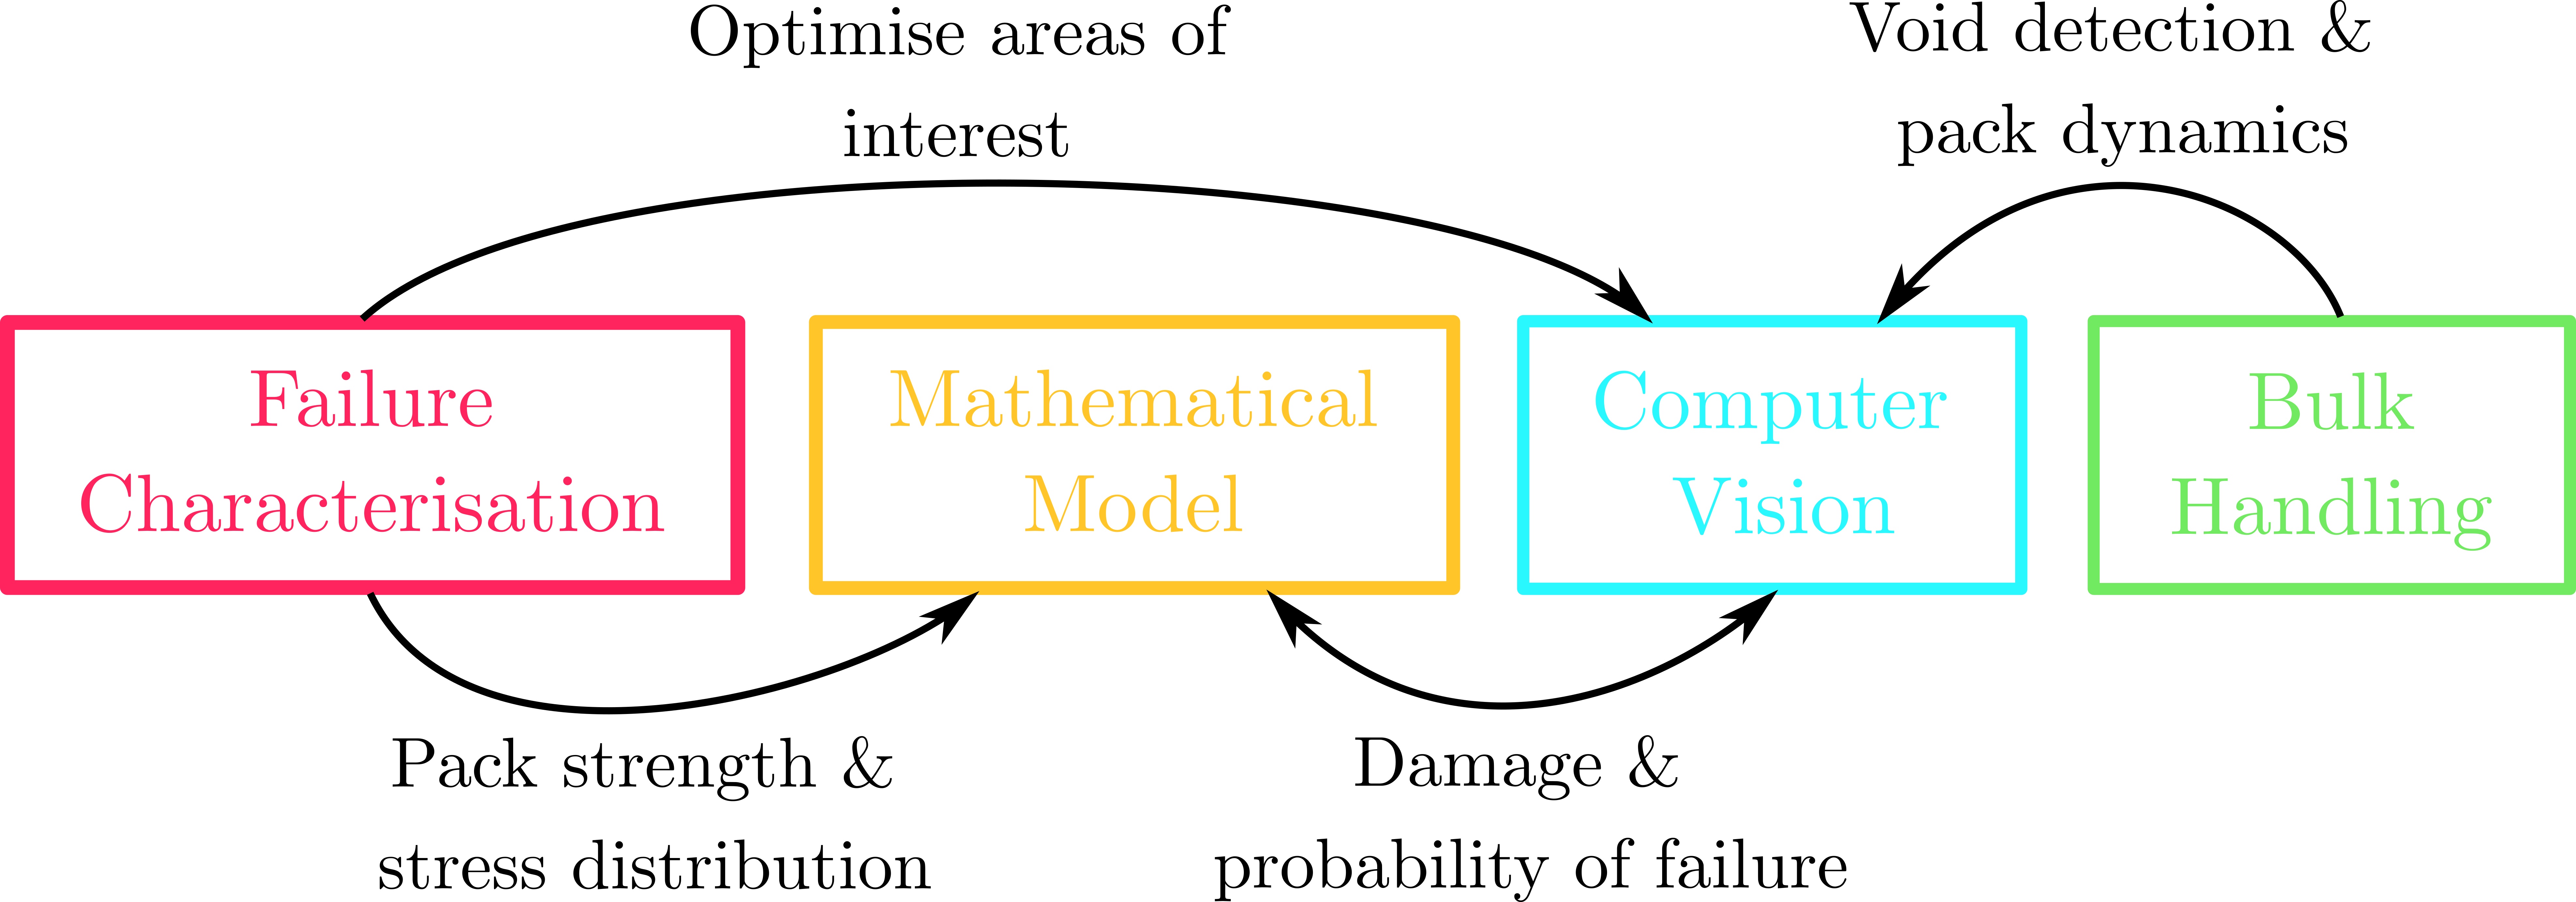
\includegraphics[width=1.0\linewidth]{images/System_Diagram.png}
\caption{System diagram of group project components}
\label{fig:SystemDiagram}
\end{figure}
\vfill

\clearpage
\subsection{Project Objectives}
The project's core objective is to design an image processing pipeline for production line health monitoring. To help make this more achievable, a list of sub-objectives was produced to provide greater structure and better clarify the scope of the research project. These objectives are presented below:

\begin{enumerate}
    \item Gain a baseline understanding of the state of monitoring techniques through a review of academic papers and commercial solutions. This is important to streamline solution synthesis, allowing for existing solutions to be applied and modified to help solve the domain-specific challenges associated with the project.
    
    \item Build a data generation utility to provide a source of rich data for developing and validating the computer vision pipeline. This is particularly important given the absence of physical samples and real-world production line footage, allowing for development work to proceed despite these limitations. This will also facilitate the provision of accompanying ground-truth data with little further effort, unlike a traditional data collection exercise.
    
    \item Implement detection functionality, allowing for individual packs to be localised in the scene and used for tracking efforts and to quantify spatial relations between packs. The detector should be capable of near real-time operation and should operate at a high level of accuracy for most relative and informative insights.

    \item Implement tracking functionality, allowing packs to be consistently identified along the line, and thereby providing motion history information for filtering high-risk packs. This should be capable of near real-time performance, and should be robust, allowing for more prolonged tracking and acquisition of data. It should also be able to track candidates with similar or identical appearance.
    
    \item Design and implement domain-specific health assessment procedures to quantify line health at a sample and population level. This will provide an insight into the formation of failure events, and facilitate automated detection and extraction of these events with further work. These processes should be highly performant (near real-time) to remain relevant and should be designed to capture the key failure modes on the line (tipping and crushing).
    
    \item Evaluate the system components to quantify the level of performance than can be expected from the proposed methods, with a comparison against ground truth measures and real-time performance standards to identify an optimal technique where multiple approaches are presented. An overall evaluation of the pipeline will also be conducted to understand the overall capabilities of the presented system.
    
    \item Evaluate the findings from the research and modelling work, considering the key outcomes and commercial applicability of the activities. Scope for further development will be considered, as well as outlining the influence of this research project on the development activities in the second year of the design project.
\end{enumerate}


\clearpage

\section{Literature Review}
\subsection{Current State of the Industry}
Production systems are complex entities and require sophisticated monitoring and inspection processes to maximise product quality and yield. Traditional production tracking was highly manual, with a process manager logging system-wide performance information on a central production board. While providing some centralised monitoring capabilities, these manual methods were highly flawed, with the need for a human operator resulting in limited consistency, reliability, and scalability.

Automation of these inspection and monitoring processes followed through the adoption of electronic record-keeping and sensor-driven monitoring \cite{deloitte-sensor}. This provided round-the-clock operation, improved quality and consistency of logged information, and improved data synchronisation over the manual counterpart. However, one of the largest challenges associated with sensors is the reduced flexibility of operation over a human operator, requiring careful selection of appropriate sensors and processing algorithms to capture the same information, especially where a more abstract measurement is required.

The most common type of sensor used in production lines environments has traditionally been the photoelectric sensor \cite{photoelectric}, with applications in product counting and occupancy detection due to their high precision, high-speed operation, and suitability for sensing transparent surfaces. The main drawbacks to these simple sensors are their operational limitations, only being suitable for single-file monitoring applications and producing spatially-discrete scalar measurements, thereby requiring numerous sensors to monitor a larger region.

Radio Frequency Identification (RFID) tags have also been widely used within industrial monitoring applications \cite{rfid}, taking a different approach to device monitoring, with on-device integration as opposed to external sensing. This allows them to store device-specific information, such as quality control or inspection data (when coupled with other sensors), and allows devices to be uniquely identified for improved traceability and factory-wide tracking \cite{brusey2009effective}. RFID technology is largely limited by the need for the addition of an RFID tag per device, which can be difficult to integrate with the product, especially for a vial, and made more complicated by the need for sterility which this could jeopardise. Further limitations arise from the additional infrastructure required to interface with and read from the RFID tags, contributing to an additional expense, as well as spatially and temporally discretising the data, with transmission only possible at an RFID read station.

SmartSkin \cite{smartskin} is a commercial offering specifically developed for production line applications, consisting of a wireless drone pack equipped with sensors to continuously log and report operational conditions throughout the line, including position, speed, and pressure readings. The integration of all these sensors provides a unified approach to monitoring, as well as continuous visibility throughout the line, improving upon the simpler RFID monitoring approach. However, this technology is similarly not without fault, with the drone pack being a separate device which adds logistical challenges regarding the separation of this device from the market-ready flow. Further to this, there is a reliance on using enough drones to receive an adequate representation of the line characteristics, which itself is hindered through the high price of these devices.

Image and video processing techniques are an alternative approach to monitoring \cite{radu2014image}, and one that is gaining increasing popularity due to the richness of the visual data, and the close approximation to the analogous vision-based analysis that would be expected from a human operator. Additionally, these approaches help to overcome the limitations associated with other sensing approaches, namely the single-file restriction of photoelectric sensors (camera systems provide a larger rectangular field of view), and the coupling between product flow and sensor count associated with RFID tags and drone packs (camera systems operate remotely and so can monitor multiple devices). Computer vision techniques have traditionally been used for simple inspection purposes, such as for checking occupancy, orientation, or basic indicators of product quality \cite{cabral2015intelligent}. While capable of assessing a lot of different measures, traditional imaging systems have needed precise and consistent conditions and entirely hand-crafted detection pipelines, resulting in expensive setups, and long and labour-intensive development processes with tight operating windows.

Recent developments in machine learning have vastly improved the capability and robustness of imaging systems \cite{o2019deep}, reducing the need for the environment to be controlled to the same extent, and thereby reducing the cost and barrier to adoption. At the same time, data-driven approaches have allowed for more sophisticated algorithms, such as enabling the detection of complex product imperfections \cite{lien2018product} with greater robustness than before. While highly attractive developments, the main drawback to these data-driven techniques is the need for lots of data, which is time-consuming to collect and annotate manually, and in some instances, may not be possible without further insight. Commercial offerings such as Roboflow \cite{roboflow} and Amazon Mechanical Turk \cite{mturk} have emerged to help address this challenge by expediting the annotation process through user-friendly interfaces, distributed workloads and automated utilities. While relatively simple, these tools have garnered a lot of interest and uptake, with Roboflow recently receiving a \$2.1M investment \cite{roboflow_news}, helping to illustrate the increasing demand in computer vision systems, and hinting at the vast potential if further developed to tackle specific industrial challenges.

Despite all the advancements in image processing, most solutions currently offered are either overly specific and narrow in scope (e.g. per-device crack detection systems), or excessively abstract and lacking in task-specific analytical capabilities (e.g. generic object detection systems). This highlights a gap in the market for an intermediary system which provides the high-level large-scale detection capabilities expected for macroscopic operation, in addition to a supplementary analysis layer for domain-specific health insights. Such a system would retain a high degree of modularity and flexibility, with ease of implementing further health measures as appropriate, presenting an attractive business case both in the immediate and distant future. This forms the focus of the research project, with the remainder of the literature review considering the techniques and technology required to realise such a system.

\subsection{Methodology Scoping}
Visual data is typically provided in the form of images or videos, which would be ultimately sourced from a camera device. Typical cameras operate at a resolution of 1080p (or 1920x1080 pixels) and a frame rate of 30 FPS (frames per second) \cite{liu2013intelligent}. Camera focal length can be varied based on application, with a shorter focal length providing a wider field of view, but greater distortion, and vice versa. A focal length of approximately 50 mm is deemed similar to the human eye, and can be used to achieve a life-like representation \cite{neale2011photogrammetric}. In a typical data collection exercise, a large volume of images would be captured with the camera, and subsequently annotated with bounding box locations to denote the location of objects within the image \cite{hanbury2008survey}. This is highly time-consuming in both acquiring the raw data and annotating it, necessitating improvements to data collection to reduce the barrier to entry. 

Data augmentation is a technique used to help reduce the volume of raw data collection required, which works by extending the dataset with slightly modified versions of the input data (such as a modified brightness, colour or image scale), thereby artificially increasing the amount of data available for training with \cite{shorten2019survey}. While improving the efficiency of the data collection exercise, it still requires real-world data, which can prove difficult to obtain in large quantities due to logistical issues or time constraints. Synthetic data is a popular solution to this, using general-purpose tools (e.g. Blender \cite{sieczka2020blender}, Unity \cite{tremblay2018training}\cite{wang2021pixel} and Unreal Engine \cite{qiu2016unrealcv}\cite{wang2019learning}) or more industry-specific offerings (e.g. Nvidia Clara for healthcare \cite{clara}, Nvidia Drive for autonomous vehicles \cite{drive} and Nvidia Isaac Sim for industrial robots \cite{isaac}) to produce a digital proxy for the real environment. This helps to speed up the collection process and provides additional control over environmental parameters, allowing for a larger and more varied dataset to be collected, which is demonstrated to improve performance of deep learning techniques.

Object detection refers to the act of localising (and classifying) objects within an image, often through the use of a rectangular bounding box. Traditional approaches used hand-crafted features for detection, such as matching colours \cite{hamuda2017automatic}, shape \cite{leavers1992shape}, or even a reference template image \cite{briechle2001template}, which a rectangular bounding box could subsequently be fitted to. These methods are simple, resource efficient, and relatively fast, however their lack of flexibility and need for manual tuning results in a need for consistent imaging conditions and extended development effort. Deep learning approaches have found much success within the domain of computer vision, achieving state-of-the-art performance across a range of detection benchmarks \cite{o2019deep}. Early data-driven approaches were relatively slow, requiring multiple passes on the image to extract likely regions of interest, classify these, and then predict predict a suitable bounding box \cite{ren2015faster}. Speed improvements were achieved by merging these operations into a single pass, leading to the development of the single-stage object detector network. YOLO (You Only Look Once) \cite{redmon2016you} was one of the first detection models capable of real-time (30 FPS) operation, albeit suffering an accuracy penalty as a by-product of the performance optimisations. Further developments have improved the accuracy of these methods and their ability to detect small objects, with the Scaled-YOLOv4 network \cite{wang2021scaledyolov4} being the state-of-the-art in object detection tasks at the time of writing. Deep learning approaches have largely superseded traditional image processing techniques due to their increased robustness and flexibility, however they require large datasets to train effectively, are less interpretable than their manual counterpart, and have increased computational requirements. Further developments in deep learning architectures have led to systems which are capable of detecting 6 degree-of-freedom orientation of objects \cite{pavlakos20176}, and even detect transparent mediums (such as glass) \cite{lai2015transparent}\cite{khaing2018transparent}. This further highlights the potential for data-driven detection methods, however become increasingly complicated and less performant, and so will be not be of interest for this scope of work, with an emphasis on near real-time performance.

Object tracking techniques address the problem of tracking and consistently identifying a set of objects within a video sequence, and has also attracted a lot of research interest. In the classical tracking-by-detection approach, a set of detections in two adjacent frames are compared using similarity metrics such as spatial positioning or appearance, which can be used to assign IDs in such a way that the cost of the similarity metrics is minimised. Popular multiple object tracking techniques include SORT (Simple Online Realtime Tracking) \cite{bewley2016simple}, IOU (Intersection-Over-Union) tracking \cite{bochinski2017high} and centroid tracking \cite{nascimento1999algorithm}, using simple distance and overlap measures to compute similarity and solve the assignment problem. The simplicity of these methods results in a high performance and ease of implementation, however they can struggle with extended occlusions and other complicated tracking scenarios. Deep learning techniques have shown promise to resolve this issue, with Deep SORT \cite{wojke2017simple} adding a data-driven appearance metric to help with consistent ID allocation. While the contribution of an appearance metric is useful for tasks with objects of different appearance, this is not applicable for the intended use case in the factory (with similar appearances expected), and so the extra complexity is deemed inappropriate. A promising alternative looks at combining the detection and tracking steps into one simultaneous prediction task \cite{sun2020simultaneous}, predicting object locations, as well as motion through the use of anchor tubes (a means of characterising object trajectory). While this method is shown to perform well, it adds excessive complexity through the integration of the detection and tracking stages into one model, thereby complicating the subsequent analysis procedures, and further complicating dataset creation due to its specific requirements.

The proposed system would also require a means of analysing the risk of crushed glass and pack tipping events. Cracks within a glass container can eventually lead to catastrophic failure or glass particle generation, which should be avoided. Bump check cracks are a type of crack caused by mechanical bumps and contact between devices \cite{schaut2017enhancing}. Collision detection techniques would be required to identify these bump check events. The majority of visual collision detection approaches use trajectory-based methods to forecast and avoid collisions \cite{veeraraghavan2003computer}\cite{lai2011airborne}, motivated by their use in autonomous vehicle applications. Acceleration-based approaches to collision detection are also shown to be successful \cite{speleers2019acceleration}, and would be better suited to the intended application of detecting and analysing collision events that actually manifest. Toppling detection has been the focus of research for human fall detection, using motion cues and classification techniques to characterise the event \cite{rougier2007fall}. While successful for its intended domain, it may not be applicable for a fast and continuously moving scene, such as a production line environment. Orientation detection systems \cite{pavlakos20176} similarly show some potential for detecting toppling events, however remain restrictive based on data requirements and computational performance. Density estimation is an attractive alternative method that could be used to characterise the risk of falling within a crowded scene. These techniques typically characterise an image based on the number of instances present per unit area over the whole frame or region of interest \cite{velastin1994automated}\cite{abbas2013real}, thereby lacking the level of spatial information that is desired. A Voronoi tessellation approach to spatial distribution analysis \cite{duyckaerts2000voronoi} is better suited, capable of producing a detailed density map with a more direct applicability to localised toppling detection.

\subsection{Approach to Implementation}
Informed by the literature review, this project will adopt a synthetic approach to the development and tuning of a visual analysis pipeline, benefiting from the increased data availability this provides. A core detection and tracking capability will be central to the approach, which will be selected on the basis of an empirical comparison of techniques where high performance and accuracy are favoured. A subsequent analysis layer will be developed to assess the risk of crushed glass and toppling vials through an acceleration-based collision detection method and detailed density estimation technique respectively. 
\clearpage

\section{Research Methodology}
\subsection{Methodology Overview}
The aim of this project was to develop a computer vision system to extract health metrics from production line video footage. This could be broken into four distinct modelling stages, as follows:
\begin{compactenum}
    \item Synthetic generation of production line footage to form the target for analysis
    \vspace{0.2cm}
    \item Object detection of vial instances to provide spatial information about line state
    \vspace{0.2cm}
    \item Object tracking across frames to provide temporal information about object motion
    \vspace{0.2cm}
    \item Extraction of metrics and analysis of line health using visual spatio-temporal measures
\end{compactenum}

\vspace{0.3cm}
\begin{figure}[h!]
\centering
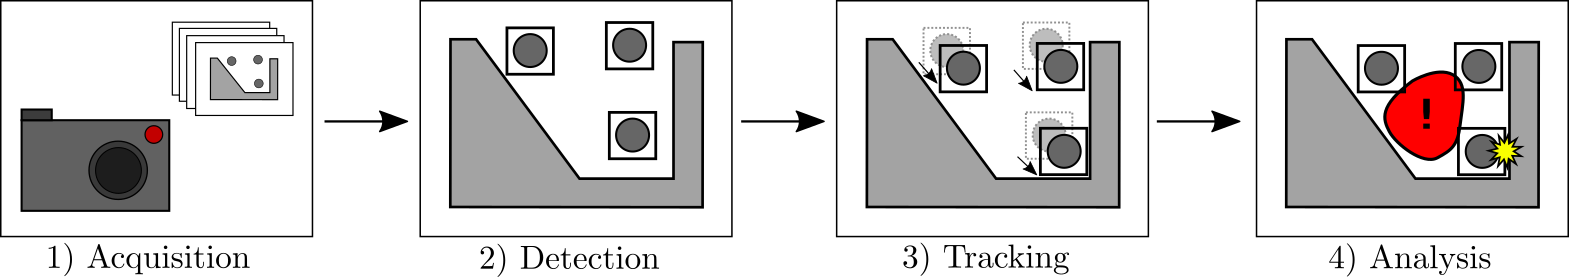
\includegraphics[width=\textwidth]{images/Methodology_Crop.png}
\caption{Diagrammatic overview of research methodology}
\label{fig:ResearchMethodology}
\end{figure}

Figure \ref{fig:ResearchMethodology} provides a graphical illustration of the project methodology, with each stage sequentially built upon the last to provide the required functionality. This thereby defined the order of modelling activities, starting with the creation of data, and later concerning the extraction of metrics and insights from this.

\subsection{Selection of Modelling Tools}
In order to achieve the outlined project objectives, an appropriate selection of modelling tools was required. Ubuntu \cite{ubuntu} was selected for the operating system due to it's low overhead, free licensing model, and high degree of compatibility with various software development libraries and hardware platforms. Python \cite{python} was chosen as the primary programming language as a result of its versatility, accessibility and wide assortment of libraries, with notable examples including OpenCV \cite{opencv} for image processing functionality, and Numpy \cite{numpy} for fast numeric computation. C\texttt{\#} was also selected for use in the project, particularly for scripting the functionality of the virtual environment. The Unity game engine \cite{unity} was selected for this, being highly customisable, and having a competent integrated physics engine and graphical rendering pipeline.

\subsection{Data Generation}
Synthetic data generation was acknowledged as the preferred form of data acquisition during the early stages of the project. This was both to help address the difficulty in accessing real-world footage due to the inherent sensitivity of this data and logistical issues surrounding the COVID-19 pandemic, as well as to provide the additional benefits with regards to data efficiency, as outlined in the literature review. The Unity game engine was chosen for creating the synthetic environment, which would be imaged using a virtual camera. This would provide a video output similar to that expected from a real-world camera, with the additional benefit of full environmental control through user-scripted behaviours and round-the-clock availability, unlike a physical line visit. Two virtual environments were created, one producing static images for detector development, and the other generating video footage for tracker development and overall assessment of system functionality.

\subsubsection{Rendering Environment}
The rendering environment was created in order to facilitate the acquisition of ground truth data for training and evaluating detection algorithms. This included: producing a representative virtual vial geometry; curating a realistic visual appearance within the scene; implementing a suitable spawn algorithm for randomised vial locations; and enabling the output of ground truth annotations in a standardised format for subsequent detection operations. It was decided that detection efforts would be conducted in a top-down approach in order to provide full visibility of the bulk material flow with minimal perspective distortion, and so the synthetic environments were built with this constraint in mind for added simplicity.

\subsubsubsection{Vial Geometry Creation}
While all commercial vials are largely unique in geometry, they share several common features such as a wide base and narrow neck, ensuring they remain recognisable even with varying shapes and sizes. To this extent, a representative 3D model of a vial was created, drawing reference from existing vials with respect to their overall geometry and proportions to achieve relative familiarity, however not fixating on dimensional accuracy to achieve a brand and device-agnostic outcome (see Figure \ref{fig:vial_geometry}). Blender was used to create the 3D model due to its powerful polygonal modelling capabilities and its native support within the Unity game engine, allowing game assets to be automatically updated upon modification. This streamlined the development process, as well as enabling rapid exploration of different geometric variants, thereby expanding the usefulness of the data generation utilities.

\vfill
\begin{figure}[hbt]
\centering
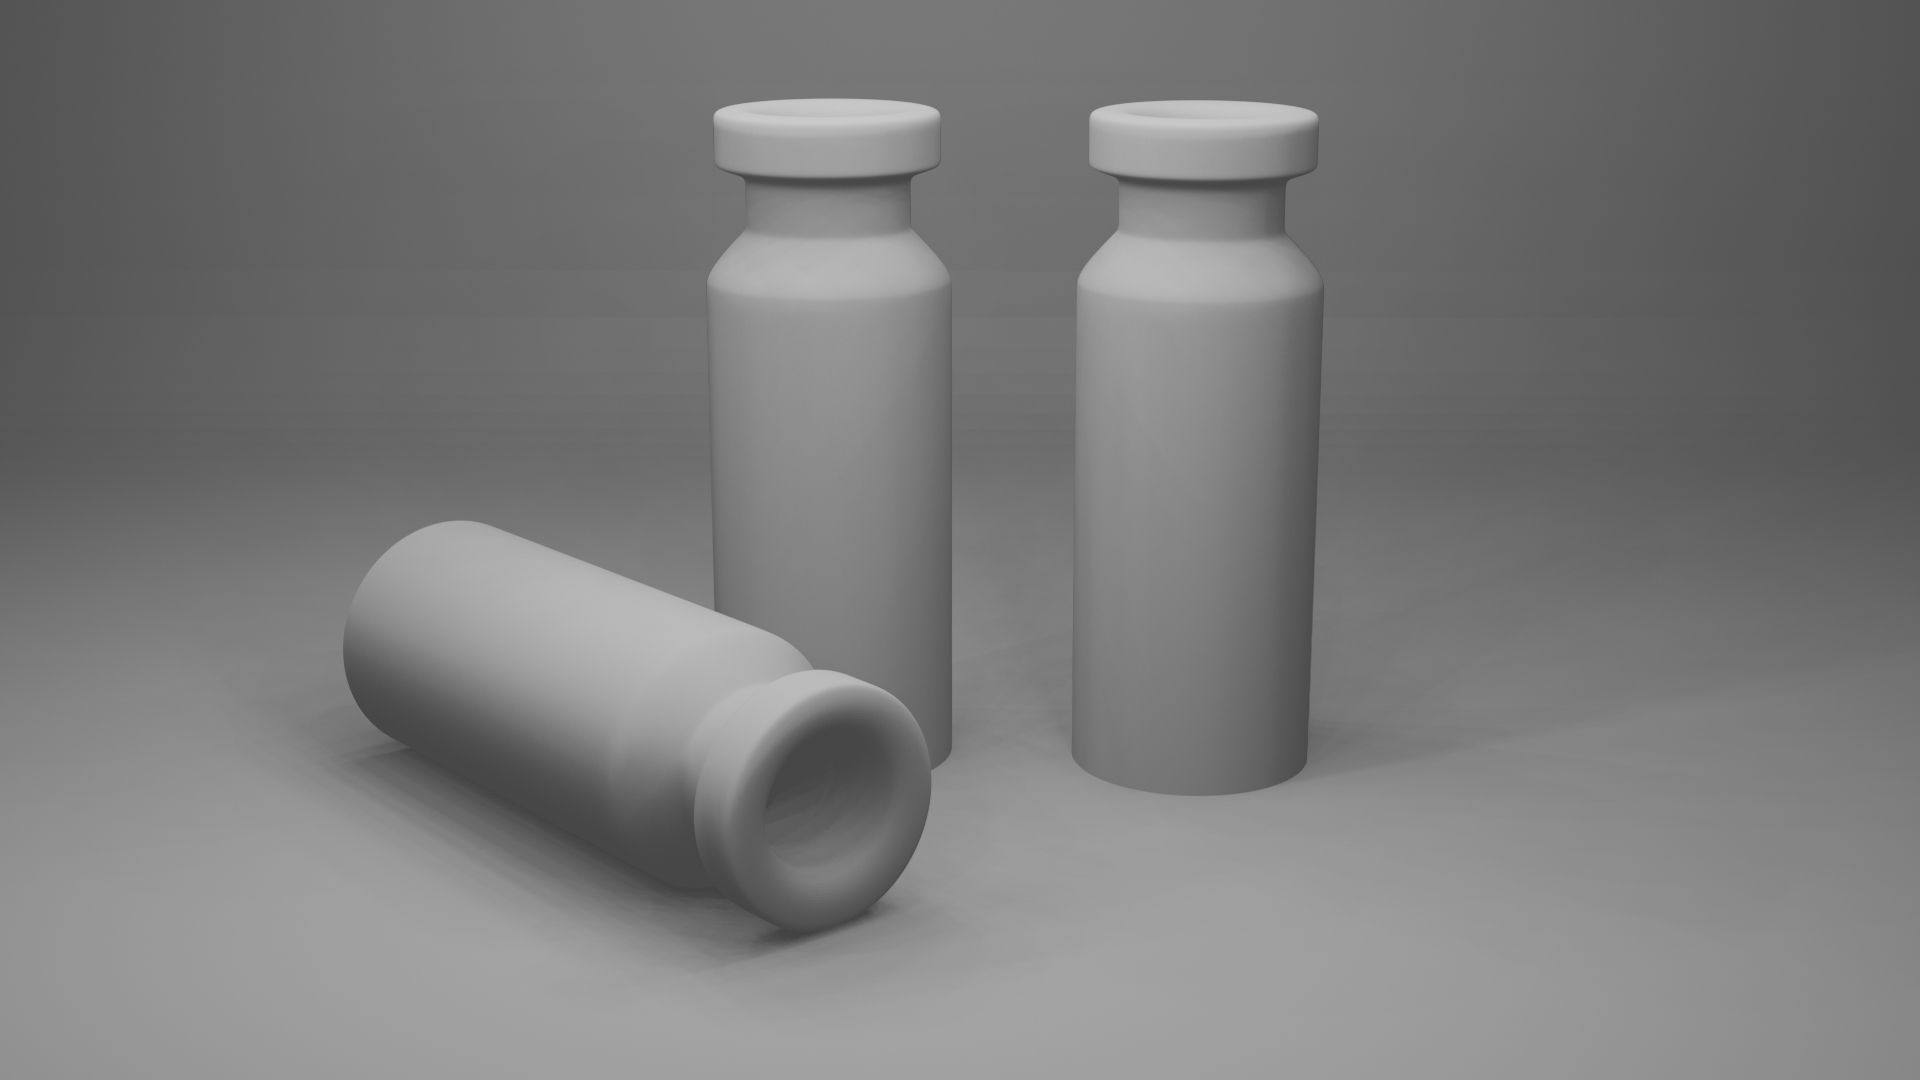
\includegraphics[width=0.85\textwidth]{images/Vial_Geometry.png}
\caption{3D model of vial created in Blender}
\label{fig:vial_geometry}
\end{figure}
\vfill

\clearpage

\subsubsubsection{Visual Appearance Curation}
Once imported within the Unity game engine, the appearance of the vial asset had to be specified. A high level of graphical fidelity was required in order to accurately assess the feasibility of the proposed workflow, which excessive abstraction of the visual appearance would serve to over-simplify.

A pseudo-glass material was created in the Unity editor to capture the general visual properties of a vial, utilising the High Definition Render Pipeline (HDRP) for greater realism. This included the allocation of a transparent surface type with alpha blending (62\%), back-then-front rendering, transparent depth prepass, and geometric specular anti-aliasing. A sphere refraction model was used with an index of refraction of 1.032 in order to capture the subtle refraction observed with a real glass vial. 

This rendering approach has its shortcomings, with a key limitation of the HDRP transparency model being the inability to render multiple transparent surfaces directly behind one another. Raytracing provides a means of overcoming the transparency limitation, however incurs large performance penalties without specialist hardware, so was omitted from the present modelling exercise. The top-down imaging approach that was adopted was deemed to help limit the impact of the transparency limitations without the performance penalty, providing a reduced ability for transparent objects to occlude each other, and hence reducing the number of cases in which these discrepancies would be observed.

Aside from directly tuning the vial material, wider HDRP settings were also configured in order to improve the overall visual fidelity and realism of the environment. The virtual camera was positioned 60 cm above the ground plane, which was deemed to be an acceptable height for a camera rig, and it was configured with a 50 mm focal length and field of view equivalent to that of the 65 mm Alexa sensor. This provides physically plausible imaging properties, akin to using the aforementioned camera, and reduces the likeliness of imaging artefacts that would not be replicable in the real world. In order to reduce the cleanliness of the image, additional optical phenomena were introduced into the virtual image capture process, namely motion blur, depth of field, and chromatic aberration, reproducing some of the ``messiness'' that would be expected from an imperfect real world camera. The combined result of the pseudo-glass material and HDRP setting adjustments can be seen in Figure \ref{fig:vial_appearance}.

\vfill
\begin{figure}[h]%
    \centering
    \subfloat[\centering Perspective view \label{fig:vial_appearance_perspective}]{{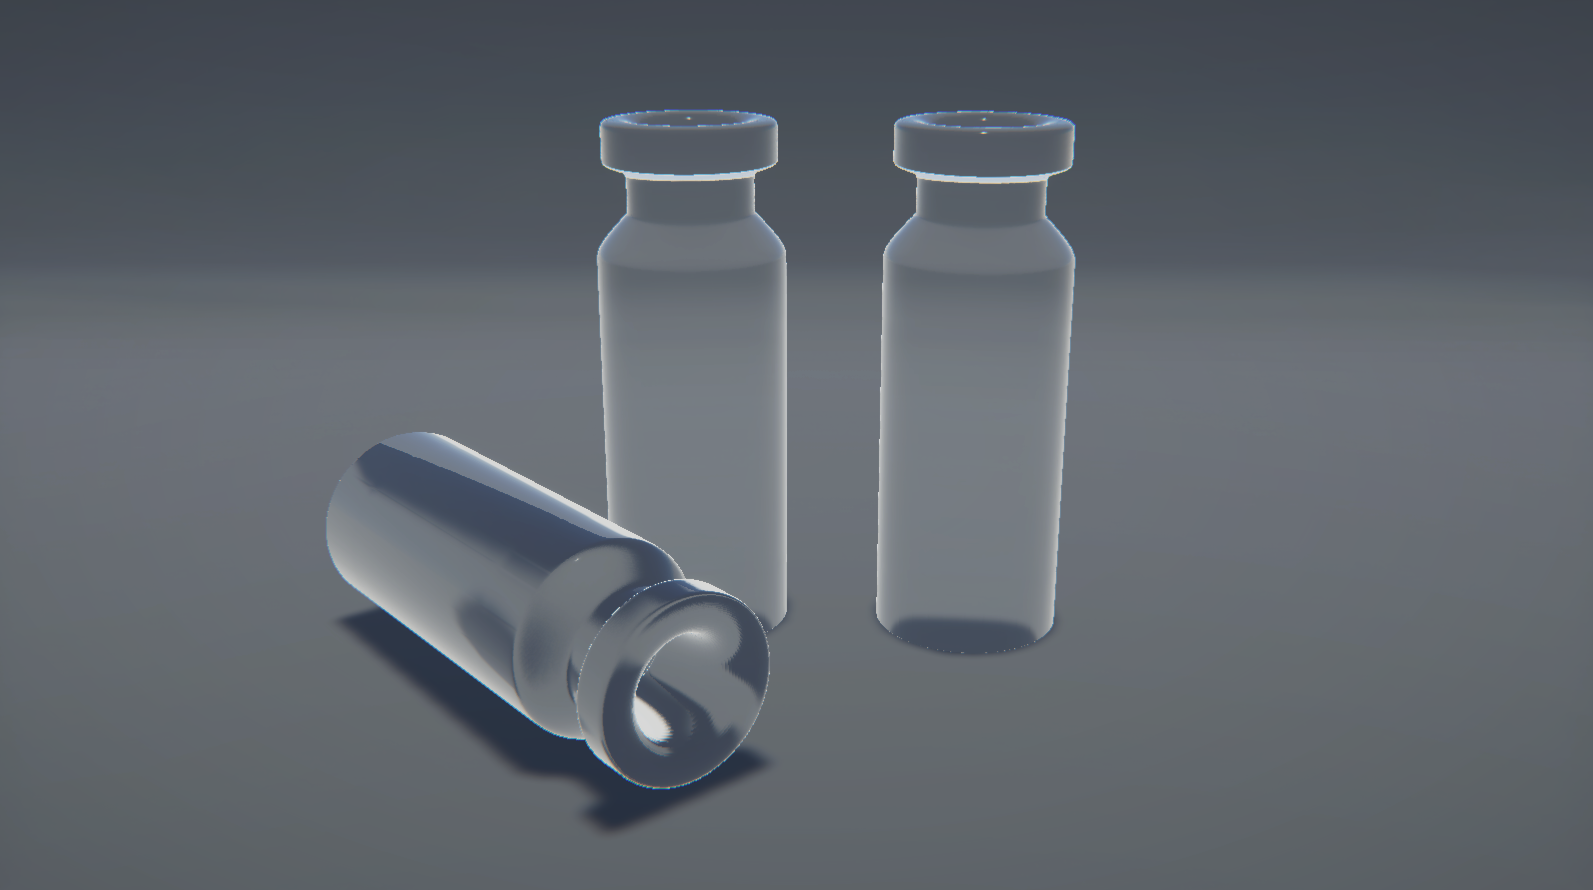
\includegraphics[width=0.47\linewidth]{images/Vial_Appearance.png}}}%
    \qquad %Add a line break to split into 2 vertically stacked images
    \subfloat[\centering Top-down view \label{fig:vial_appearance_top}]{{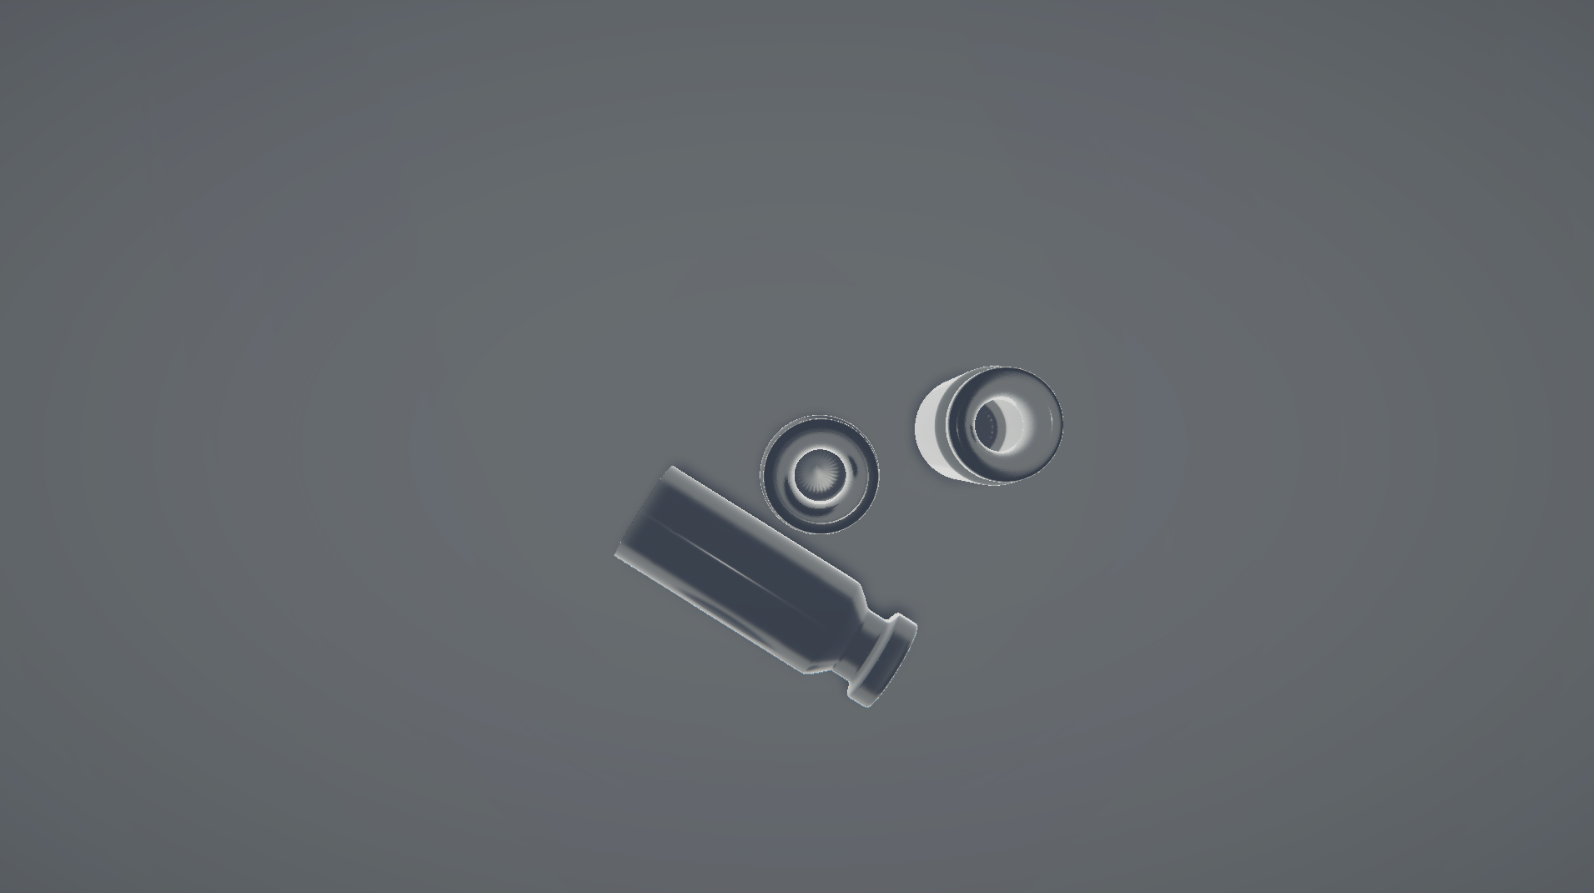
\includegraphics[width=0.47\linewidth]{images/Vial_Appearance_Top.png}}}%
    \caption{Psuedo-glass vial within Unity engine}
    \label{fig:vial_appearance}%
\end{figure}
\vfill

\clearpage

\subsubsubsection{Spawn Algorithm Design}
In order to produce an representative and diverse object detection dataset, it was important to get good coverage of different spatial arrangements of objects (known as ``GameObjects'' in Unity) within the frame. In order to facilitate this, a parametric packing routine was implemented to randomise vial placement. A combination of user-specified starting position, instance offset, and column-wise shift amount were used to defined either a square or hexagonal packing arrangement of instantiation points for the creation of GameObjects. Further randomisation was offered through the addition of a random offset in the range [-0.1, 0.1] to translate the pattern by up to a whole vial diameter, thereby allowing for full translational coverage in the image plane for additional spatial variation. Figure \ref{fig:vial_placement_hex} provides a graphical illustration of the algorithm.

\vspace{0.15cm}
\begin{figure}[hbt]
\centering
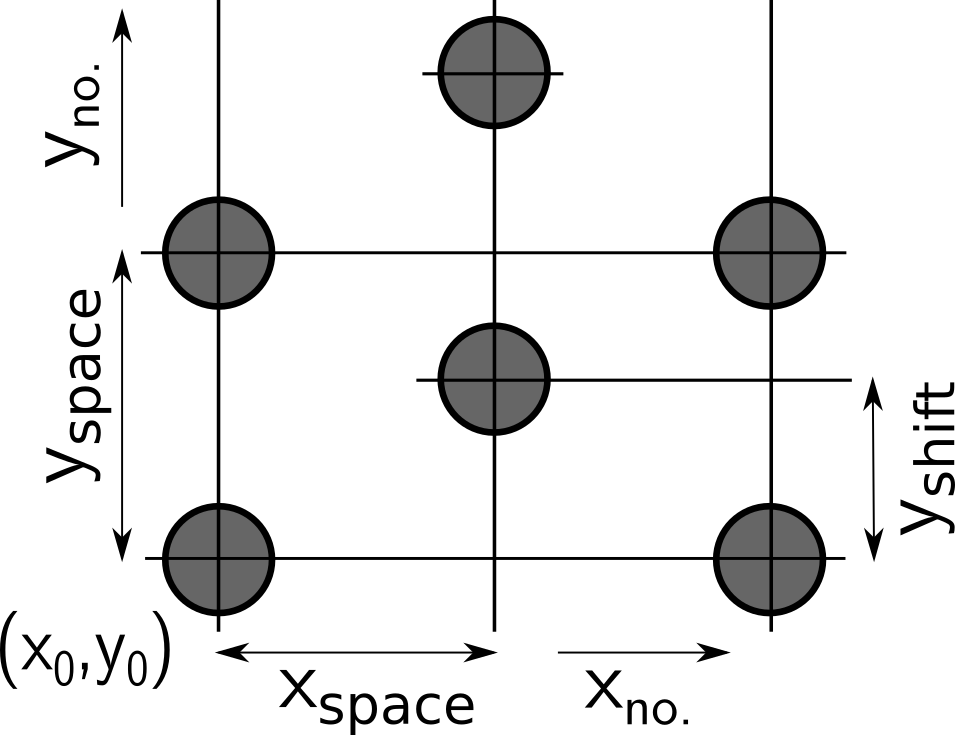
\includegraphics[width=0.45\linewidth]{images/Spawn_Hex.png}
\caption{Parametric packing algorithm overview}
\label{fig:vial_placement_hex}
\end{figure}

In order to capture a range of packing densities and object counts, different subsets of these instantiation points were selected using reservoir sampling \cite{vitter1985random}, in which \textit{k} items (user-specified) are randomly selected from a population of size \textit{n} in a single pass. This was achieved by iterating through all the points and instantiating a GameObject at a point if $\textit{Random(0,1)} < \frac{\text{Number of remaining items to be selected}}{\text{Total number of points remaining}} $. This could be repeated several times and for different values of \textit{k} to add further variety to the dataset.

\subsubsubsection{Output Generation}
The raw 3D information was incompatible with the planned image processing techniques, and so a 2D output had to be produced. This was achieved by rendering the virtual camera view to a render texture which could be dumped to a 2D image file, thereby translating the scene into a more standard 2D image representation. In addition to saving out an image file, a corresponding label file was to be generated with the ground truth bounding box information of all instances, thereby allowing for training and testing of detection algorithms. The ground truth bounding boxes were tightly fitted about the neck of the vial, with the top of the vial selected as the most robust feature to detect given its consistent appearance and resistance to occlusion (self or otherwise), unlike the base of the vial that would be hidden upon dense vial packing.

A script was written to retrieve the ground truth bounding box information. This worked by iterating through all the vial instances present within the frame, extracting the centre of each object and its render bounds (or 3D bounding box dimensions). This information could be used to locate the corner points of a bounding rectangle for the top of the vial in 3D space, corresponding to $(x_{centre} \pm x_{extents}, y_{centre} + y_{extents}, z_{centre} \pm z_{extents})$. These points were subsequently transformed from 3D world coordinates to screen space coordinates for the virtual camera by using the \texttt{WorldToScreenPoint()} method within Unity, corresponding to the pixel locations of the bounding boxes within the image. Subsequent conversion of the bounding box information to the YOLO-style notation was achieved by first converting the 2-point corner specification (x1,y1,x2,y2) to a centre and size definition (x,y,w,h), and then normalising these by dividing by the respective dimension of the image. An additional class label (constant value 0 for the single vial class) was prepended to this data, producing a finalised data line in the following format:

\vspace{-0.2cm}
\textit{\{class\_no., normalised\_x$_{centre}$, normalised\_y$_{centre}$, normalised\_width, normalised\_height\}}

A single spatial arrangement was deemed insufficient for producing a representative dataset, and so the driving script was extended to automatically repeat the data generation process for different instance counts and in different quantities. The final script was configured to output 500 samples with 5 objects, 300 samples with 50 objects, and 200 samples with 500 objects, which were automatically divided into a 70-30 train-test split for subsequent detector development. Example data is presented in Figure \ref{fig:Detector_Data}.

\vfill
\begin{figure}[hbt]%
    \centering
    \subfloat[5 objects][\centering 5 objects \label{fig:render_5}]{{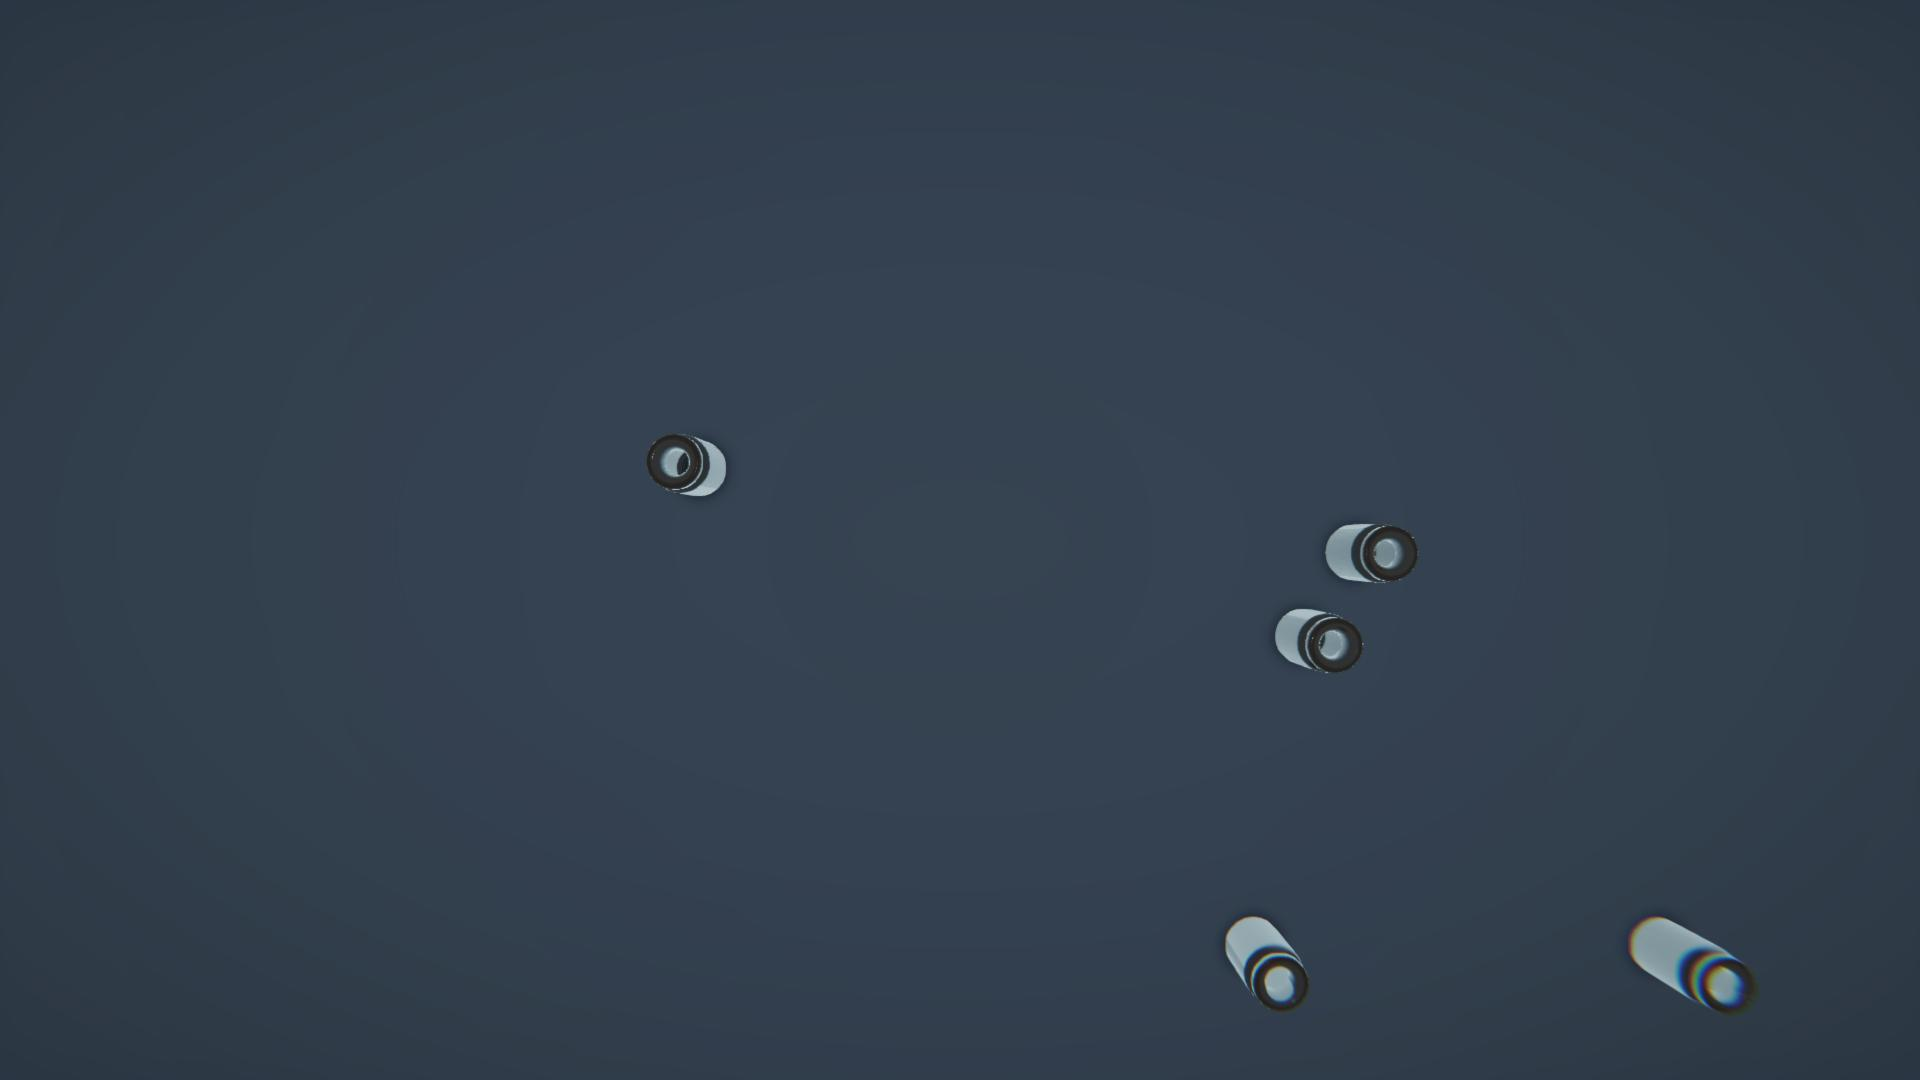
\includegraphics[width=0.45\linewidth]{images/5_45.jpg}}}%
    \qquad %Add a line break to split into 2 vertically stacked images
    \subfloat[\centering 50 objects \label{fig:render_50}]{{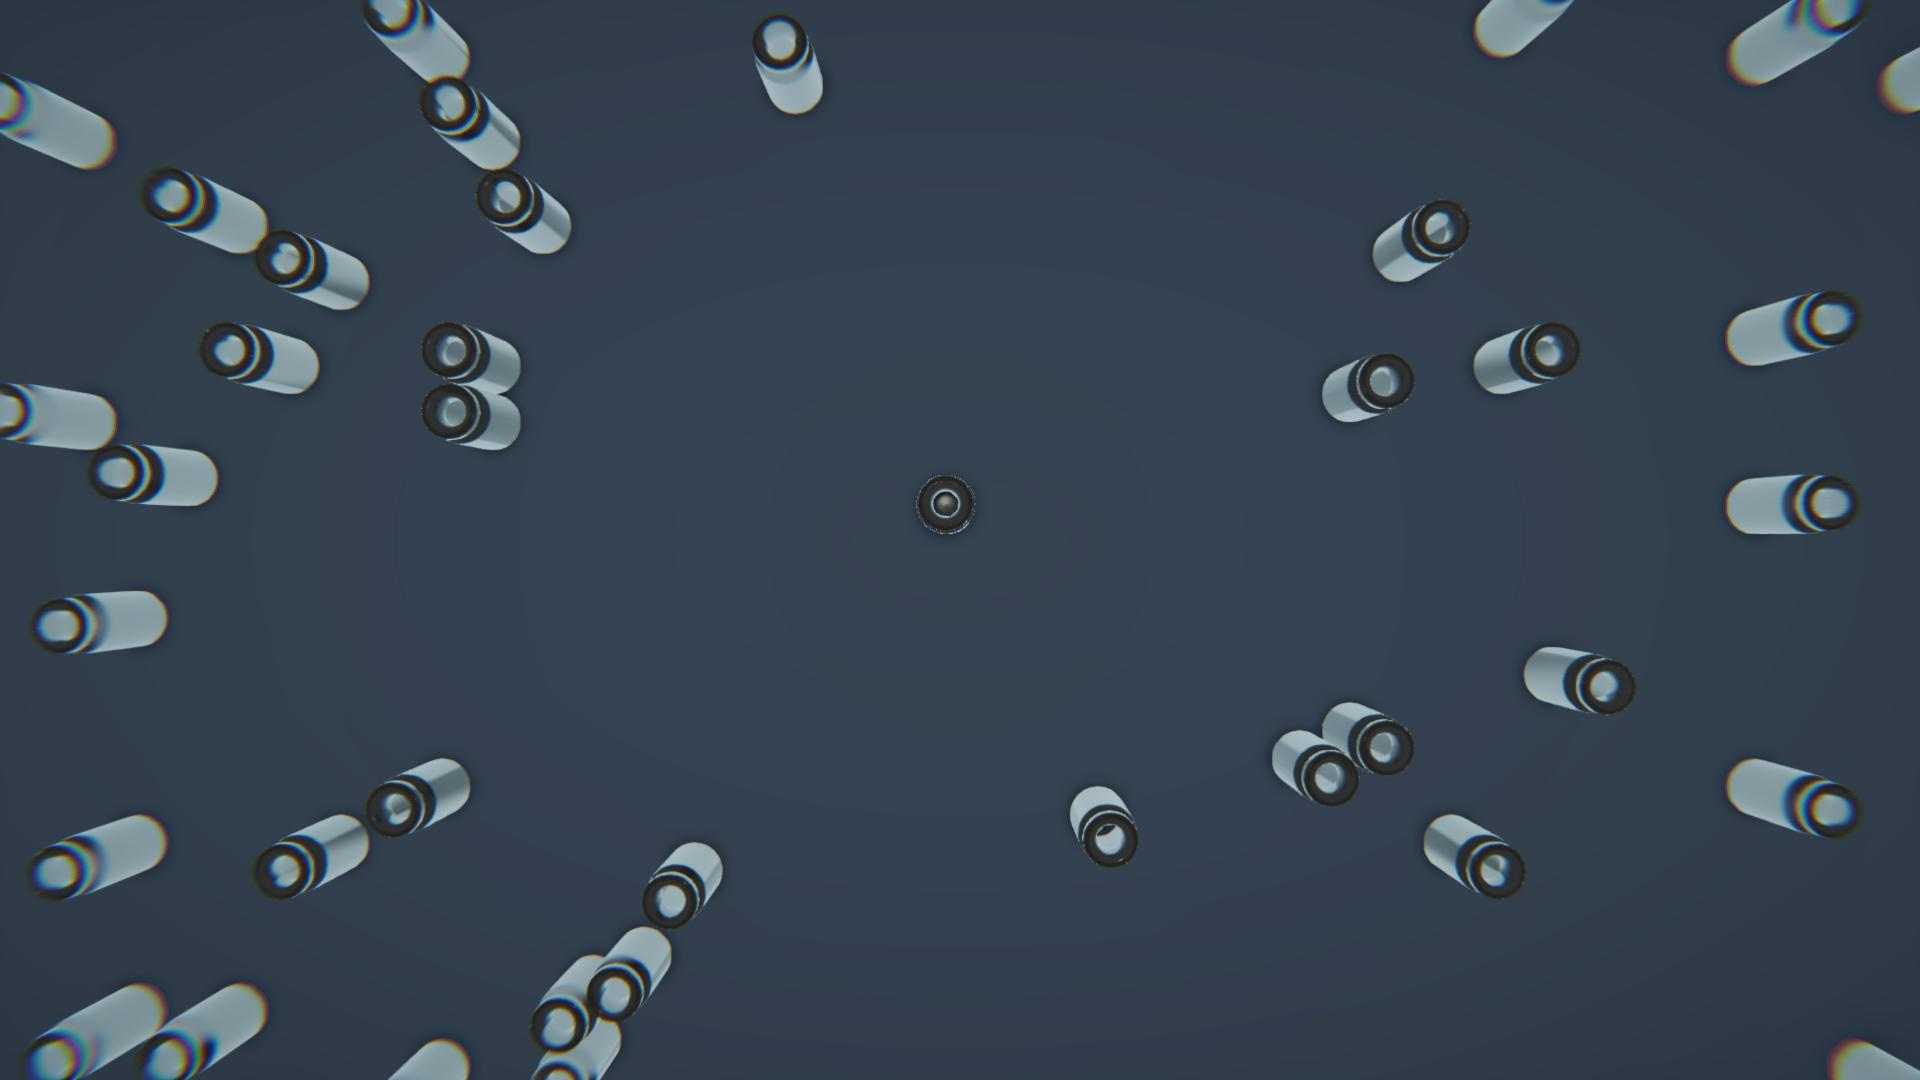
\includegraphics[width=0.45\linewidth]{images/50_9.jpg}}}%
    \qquad %Add a line break to split into 2 vertically stacked images
    \subfloat[\centering 500 objects \label{fig:render_500}]{{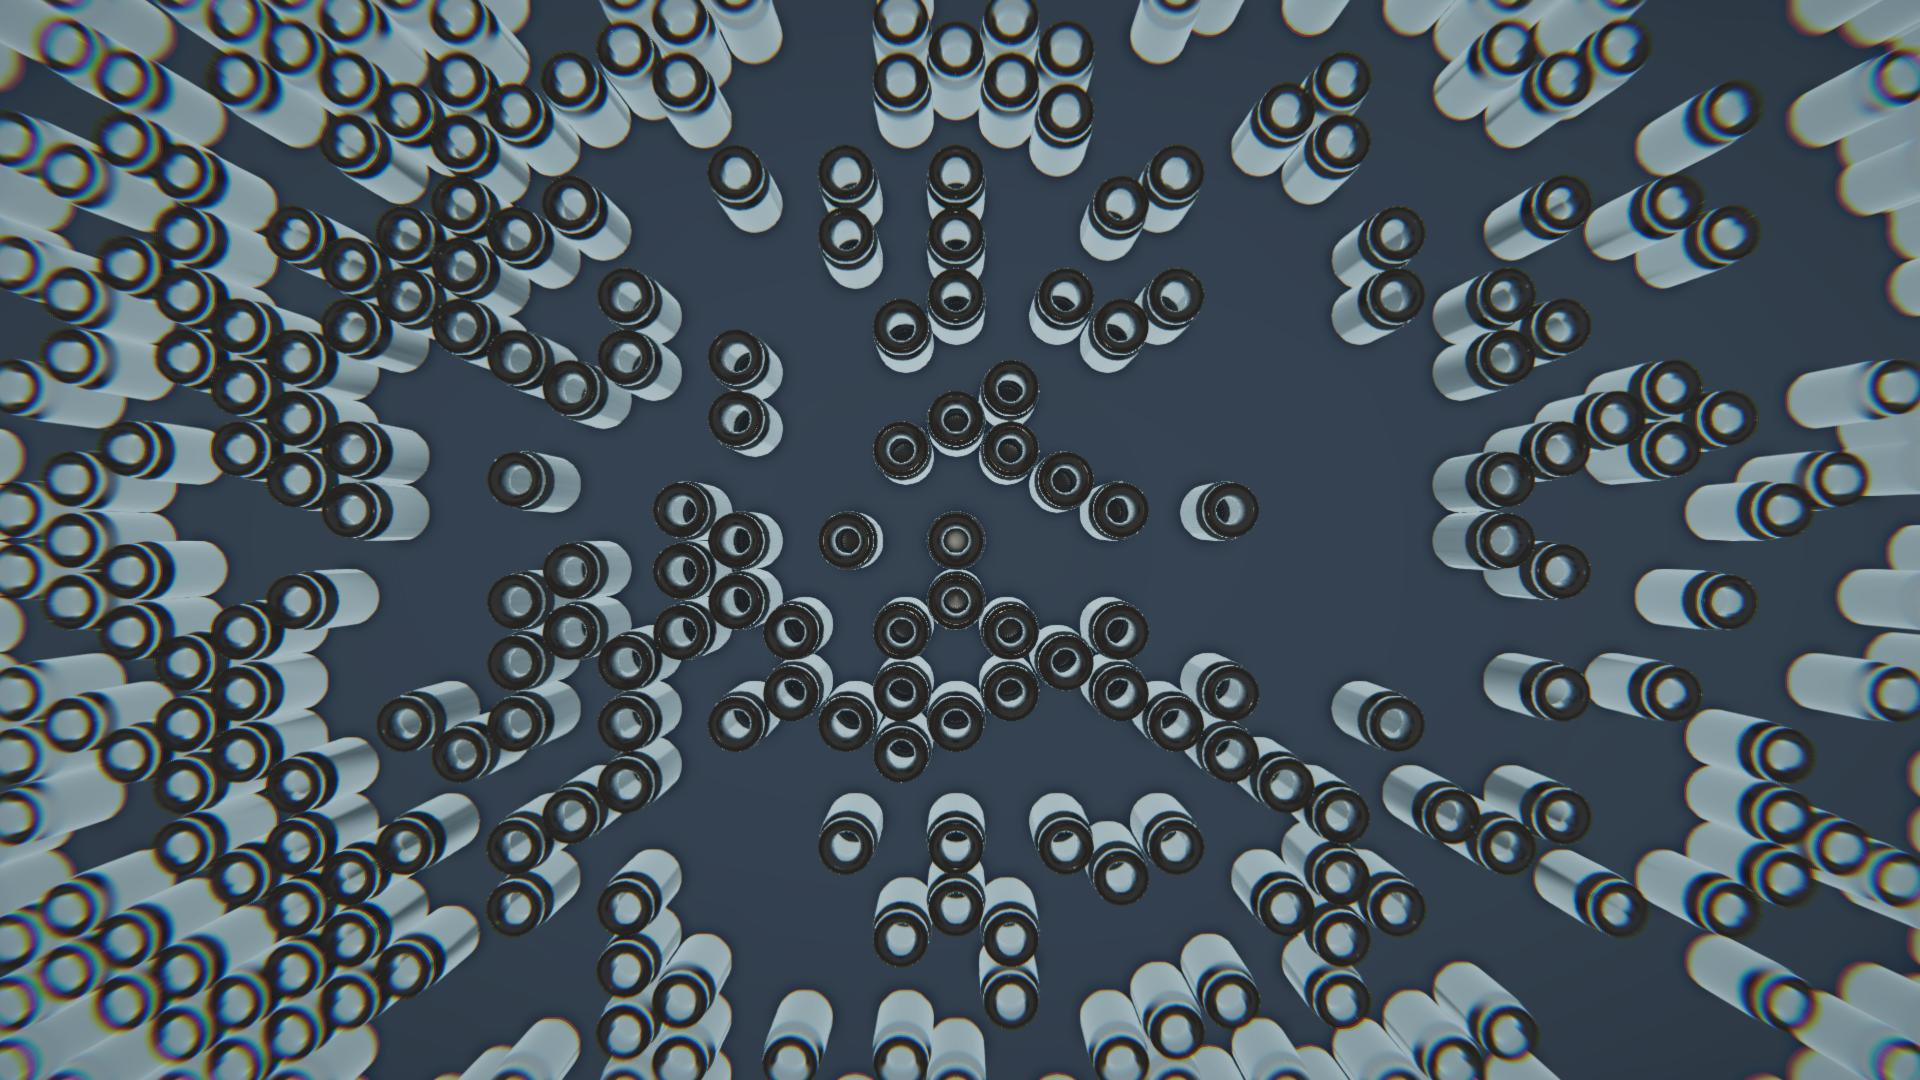
\includegraphics[width=0.45\linewidth]{images/500_39.jpg} }}%
    \qquad %Add a line break to split into 2 vertically stacked images
    \subfloat[\centering 500 objects (bounding box overlay visualised) \label{fig:render_500_img}]{{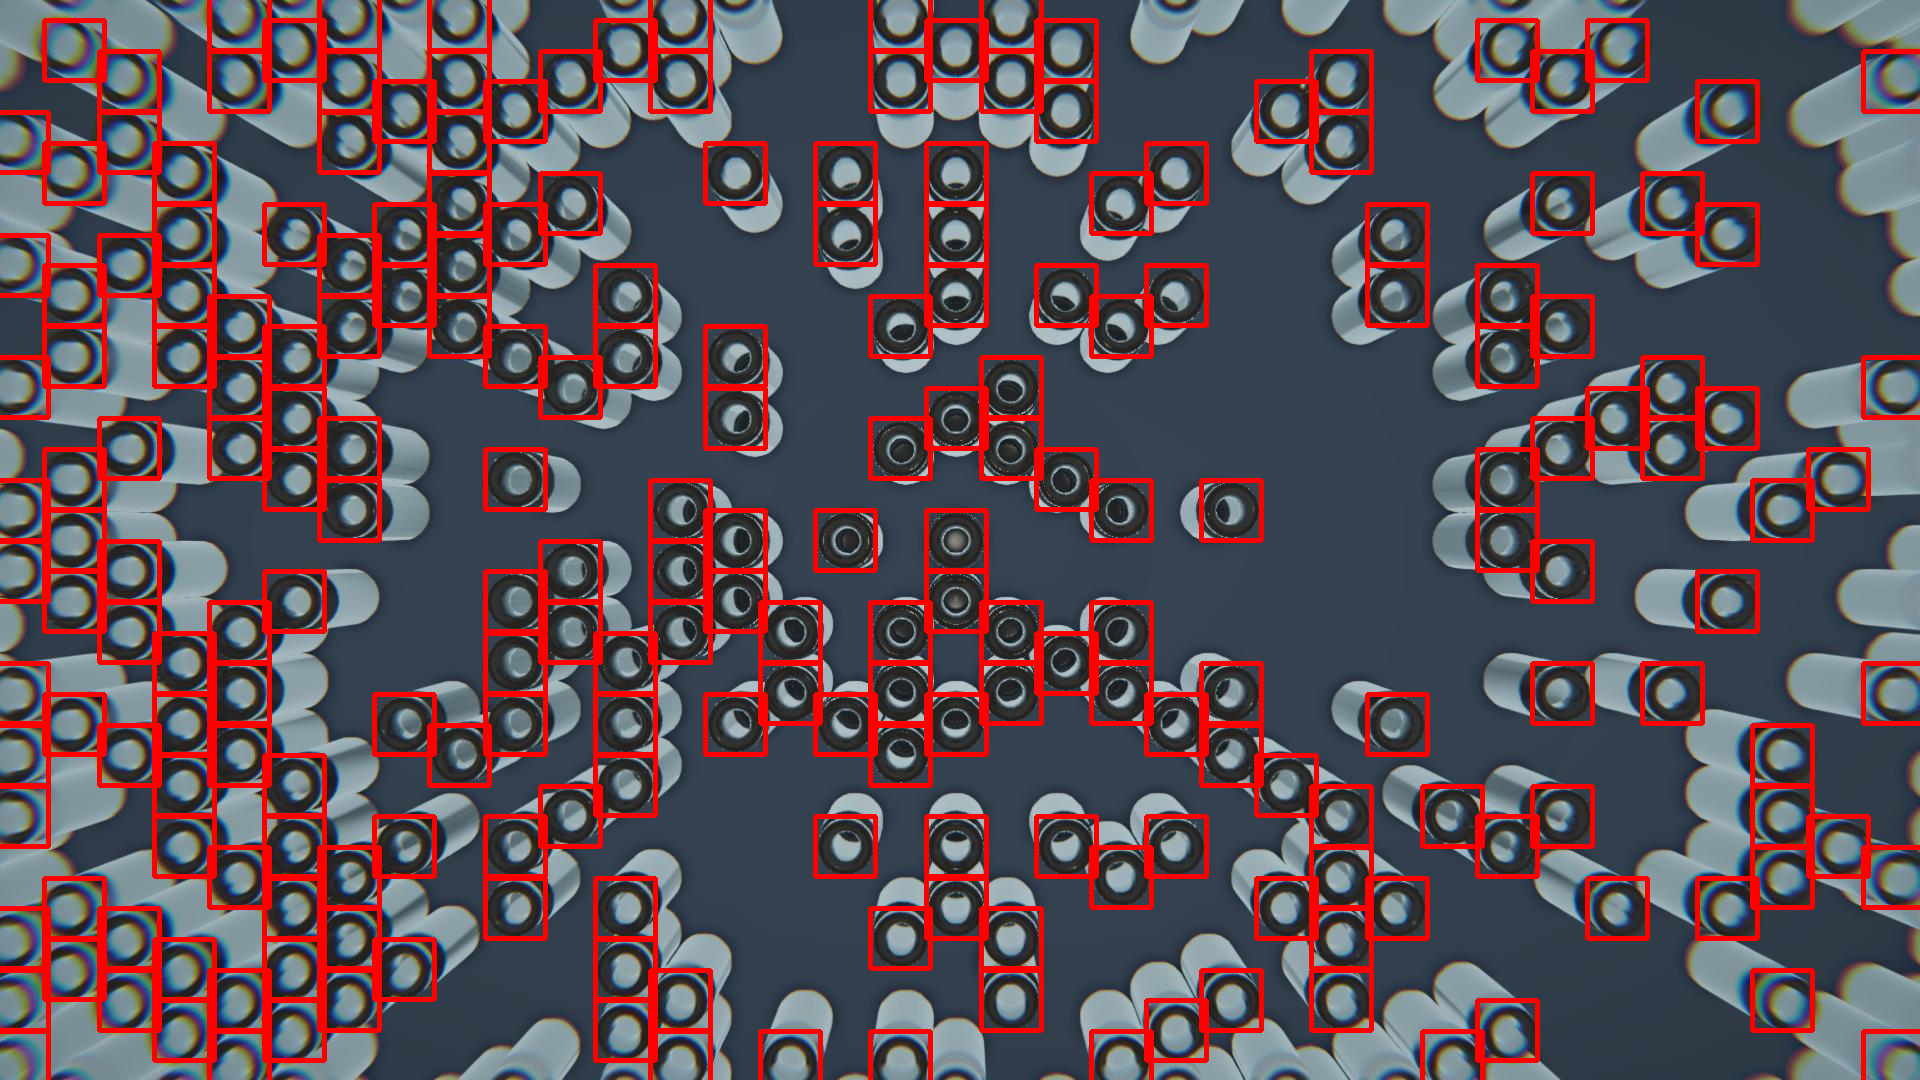
\includegraphics[width=0.45\linewidth]{images/500_39_annotate.png} }}%
    \qquad %Add a line break to split into 2 vertically stacked images
    \subfloat[\centering 500 objects (bounding box data excerpt) \label{fig:render_500_txt}]{{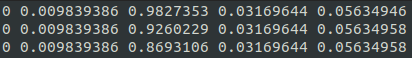
\includegraphics[width=0.5\linewidth]{images/500_39_label_ext.png} }}%
    \caption{Render environment outputs}
    \label{fig:Detector_Data}%
\end{figure}
\vfill

\clearpage

\subsubsection{Simulation Environment}
The simulation environment was created in order to provide a source of video footage for demonstrating tracking capabilities, overall system performance, and the applicability of domain-specific metrics. The simulation environment was largely an extension of the existing rendering environment, albeit with the addition of game physics to simulate approximate pack interactions and macroscopic behaviours. Development of the simulation environment required consideration of the physics setup, integration of an appropriate spawn algorithm, and suitable ground truth output logging.

\subsubsubsection{Physics Setup}
Unity's integrated Nvidia PhysX engine \cite{physx} was used to provide 3D physics simulation capabilities. The physics engine prioritises stability and computational speed over accuracy, with a primary use case being video games as opposed to physically-accurate simulations. This reduced physical realism was deemed acceptable for the purposes of the modelling exercise, with the intended health estimation workflow being scenario-agnostic and hence not being overly reliant on any specific interactions or observations that may otherwise be impacted.

A custom accumulator scenario was created (as depicted in Figure \ref{fig:simulation_scene}), with a bulk-monitoring environment selected in order to fully realise the benefits of a computer vision pipeline over a classical sensing approach. A funnel-shaped guide profile was used within the scene to encourage a dense packing of objects, resembling a crowded accumulator. A different funnel angle was used at either side in order to achieve different velocity profiles for incoming packs and to try and further randomise packing behaviour throughout the frame.

\vspace{0.1cm}
\begin{figure}[hbt]
\centering

\includegraphics[width=0.6\textwidth]{images/Physics_Setup.png}
\caption{Simulation environment}
\label{fig:simulation_scene}
\end{figure}

Regarding simulation settings, a 0.01 second timestep was used within the solver (half the default value). This was settled upon in order to improve the accuracy of the simulation and minimise inter-frame penetration resulting from the discrete collision formulation for high speed objects. A rigid body representation was used for all simulated objects, which was justified by the relatively high stiffness (and resulting low capacity for deformation) of the concerned materials. The scenario was assumed to be gravity-fed at an inclination of 20\degree{} about the X-axis, and hence directional conveying was achieved through a gravitational load with components resolved in the Y and Z directions. This provided a lightweight approximation to the gravity-fed load case, and avoided simulation artefacts resulting from improper contact computation. To this extent, a small clearance was also added between the vials and the ground plane, with the vertical translational degree-of-freedom subsequently removed from the vials in order to avoid ground contact and the problematic simulation results that would follow. All rotational degrees-of-freedom were also locked, limiting the movement of the vials to pure XZ translation. Although this limited the physical accuracy through a reduced ability for organic toppling events, it was deemed appropriate in order to negate the deficiencies of the game physics, with improper contact computation otherwise leading to excessively unstable objects when compared to a real-world case. This was not a major limitation as far as the scope of the project was concerned, with the spatial toppling formulation inspired by the literature review remaining relevant even without the possibility of directly observing toppling events in the simulation itself.

\subsubsubsection{Spawn Algorithm Design}
The physics simulation needed a means of introducing new vial instances at a regular interval, in order to emulate the batch-wise loading that could be expected on a production line. This was achieved by using Unity's \texttt{InvokeRepeating()} function with a custom spawn method to provide this periodic object instantiation. The parametric packing algorithm from the rendering environment was not reused for this purpose, opting for a 2D implementation of the Poisson Disk Sampling algorithm \cite{bridson2007fast} which packs points closely together, but not within a specified minimum distance. The algorithm works by creating a background grid to match the size of a spawn area. A random point is inserted into the grid, after which \textit{k} further points are selected from the surrounding annular disk. These are tested for validity by checking the distance between the candidate point and those in surrounding cells, thereby accelerating the search process. This is repeated until a specified limit of success points or rejected candidate points is reached, after which the list is iterated over and a GameObject is instantiated at each point. The main advantages of using this spawn algorithm in the simulation environment included the simpler control over the algorithm due to a reduced parameter set, and the increased randomness in packing arrangement which was ideal for capturing the way that variations in conveying behaviour manifest within the accumulator inlet. A graphical overview of the algorithm is presented in Figure \ref{fig:simulation_spawn}.

\begin{figure}[hbt]
\centering
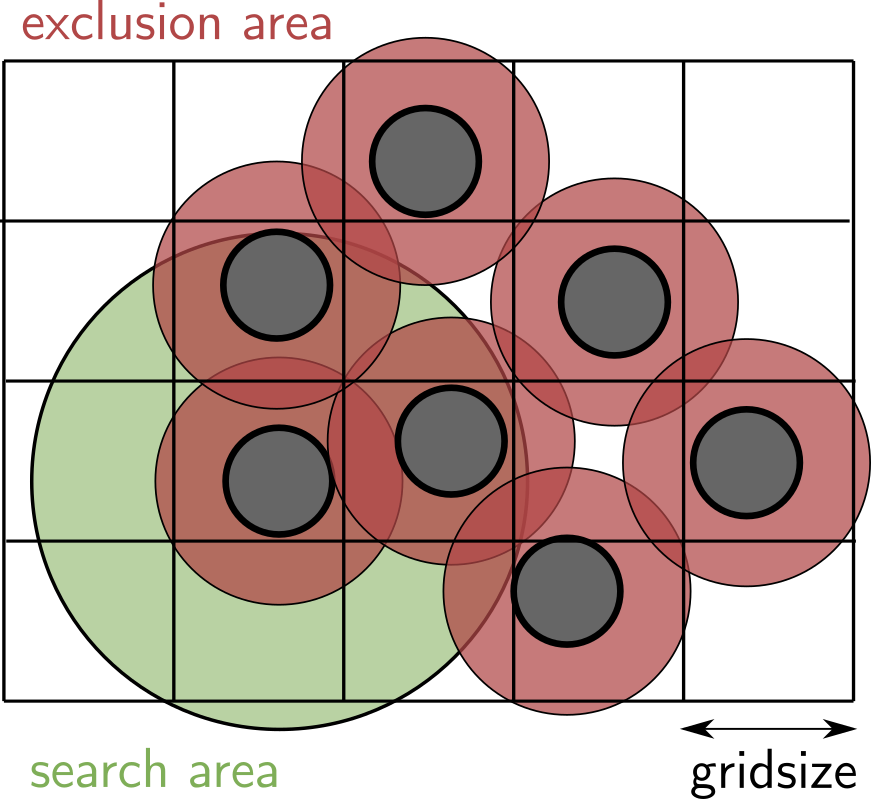
\includegraphics[width=0.44\linewidth]{images/Spawn_Pds.png}
\caption{Poisson disk sampling algorithm overview}
\label{fig:simulation_spawn}
\end{figure}

\clearpage
\subsubsubsection{Output Generation}
The simulation environment required two outputs, being video footage of the simulation taken from the virtual camera, and a ground truth data file for logging the number of vials visible per timestep. 
The video footage was produced using the Unity Recorder plugin, exporting the footage as a WebM video file and specifying a resolution of 1080p (1920x1080 px) and frame rate of 30 FPS, in line with most commercial camera solutions. The video was recorded from the main camera's field of view for a total of 407 frames, after which the scene was completely filled with vials, thereby allowing for a more comprehensive assessment of the scalability of the proposed methods. 
Instance counting was achieved by testing visibility via the overlap of each GameObject with the main camera's viewing frustum. If the two volumes overlapped, then the object was deemed to be visible from the camera, and so the instance was added to a list to keep track of these objects. After iterating through all the GameObjects within the scene, the length of the visible object list was queried, providing a count for the number of objects visible for that timestep. This was written as a new line within the data file and was repeated for the duration of the simulation, thereby providing a sequential listing of ground truth object counts for each frame in the video sequence. Example data is presented in Figure \ref{fig:simulation_output}.

\vfill
\begin{figure}[hbt]%
    \centering
    \subfloat[\centering Simulation footage (frame excerpt) \label{fig:simulation_frame}]{{
\includegraphics[height=0.22\paperheight]{images/Simulation_Pic.png} }}%
    \qquad %Add a line break to split into 2 vertically stacked images
    \subfloat[\centering Object count \label{fig:simulation_count}]{{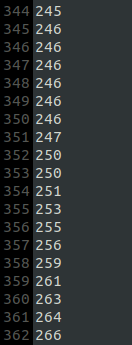
\includegraphics[height=0.22\paperheight]{images/Simulation_Data_Pic_3.png} }}%
    \caption{Simulation environment outputs}
    \label{fig:simulation_output}%
\end{figure}
\vfill

\subsection{Detection}
Several detection techniques were explored in order to localise the vials within the frame. These included traditional methods such as colour detection, Hough circle detection, and template matching, as well as the data-driven Scaled-YOLOv4 object detection method. Detector tuning was performed using the training dataset, in conjunction with supporting scripts to streamline parameter selection, template generation and generic model training. All detection outputs were returned as both centroids and bounding boxes in the 2-point format (x1,y1,x2,y2), in order to ensure consistent formatting of detector results.

\vspace{0.5cm}

\clearpage

\subsubsection{Colour (HSV) Detection}
The colour detection approach began by blurring the input image using the \texttt{cv2.GaussianBlur()} function with a 5x5 kernel in order to reduce noise and excessive detail. This was subsequently converted to the HSV colour space using the \texttt{cv2.cvtColor()} function, in order to provide greater separability of regions based on colour and brightness when compared to the standard RGB colour space. Target regions were extracted by comparing the pixel information at each point with a user-specified lower and upper HSV threshold, defined as (0, 0, 56) and (179, 94, 255) respectively, where pixels satisfying the specified range appeared as white, and those that did not were coloured black. Connected components analysis was then performed on this binary image using the \texttt{cv2.connectedComponentsWithStats()} function with square-neighbourhood (adjacent) connectivity. Each connected component was then iterated over, extracting the position, dimensions, and area, which could be used to further filter anomalous detections. This was achieved by enforcing an area constraint between 100 and 1500 pixels, with conforming regions treated as positive detections and having their bounding boxes and centroids logged.

\subsubsection{Hough Circle Detection}
The Hough circle detection approach worked by first converting the image to grayscale using the \texttt{cv2.cvtColor()} function. The \texttt{cv2.HoughCircles()} function was subsequently called, which worked by performing a Canny edge detection \cite{canny1986computational} on the image that is then converted into Hough space in order to propose circle candidates. The function additionally filtered these candidates based on additional geometric information, such as the minimum distance between detections and the size of the radius to help minimise anomalous detections. The standard Hough Detection method was used with an accumulator size 1.5 times smaller than the image size. Minimum distance between circles was set as 20 pixels, with a minimum radius of 12 pixels and maximum radius of 15 pixels. The maximum threshold for the Canny detection was set to 27 and the circle accumulator threshold was set to 19. Centroids and bounding boxes were logged for positive detections.

\subsubsection{Template Matching}
The template matching approach took an input template image and searched the frame for matching instances. This matching was achieved by using the \texttt{cv2.matchTemplate()} function with the zero-normalised cross-correlation similarity measure. The result of this comparison was a grayscale image or similarity map, where pixels with greater value correspond to a greater match with the convolved template image. A user-specified threshold could therefore be used to select matching regions, corresponding to pixel values with a value exceeding the threshold. Non-maximum suppression was included with an overlap threshold of 0.4 in order to combine detected bounding boxes where appropriate and avoid duplicate or redundant detections. The bounding boxes and centroids were logged for positive detections.

Two template images were investigated, one extracted manually from the training data, and the other synthesised automatically through a custom script. The manual (or raw) template image was extracted from the centre of the frame to capture the top-down appearance of a vial with minimal influence of perspective. On the contrary, the synthetic (or averaged) image was generated by averaging the appearance within all of the ground truth bounding boxes in the training images, thereby producing an averaged or generalised representation of the detection target. Both images were cropped for a tight bounding box, with the template images presented in Figure \ref{fig:template_images}. The raw template image used a match threshold of 0.3, while the averaged template image used a match threshold of 0.5.

\vfill
\begin{figure}[hbt]%
    \centering
    \subfloat[\centering Raw template]{{
\includegraphics[width=0.2\linewidth]{images/Template_Raw.png} \label{fig:template_raw}}}%
    \qquad %Add a line break to split into 2 vertically stacked images
    \subfloat[\centering Averaged template]{{
\includegraphics[width=0.2\linewidth]{images/Template_Averaged.png} \label{fig:template_averaged}}}%
    \caption{Template matching images}
    \label{fig:template_images}%
\end{figure}
\vfill

\subsubsection{Scaled-YOLOv4}
This detection approach used the Scaled-YOLOv4 object detection network to detect vials within the image. A YAML file was produced for the custom training scenario, using a single class with ``vial'' as the class name. As the data generator's outputs were designed with the YOLO format in mind, this data was directly compatible with the standard training procedure without further preprocessing, and so the train, validation and test directories were simply pointed to the appropriate locations. Different splits of data were experimented with, and optimal results were achieved when using all the training images for the situations with 5, 50 and 500 instances. The YOLOv4-CSP model configuration file was used to define the neural network architecture, which was then trained on an Nvidia Geforce GTX 1080Ti graphics card with 11GB VRAM. A batch size of 16 was used, with images dynamically resized to 416x416 px. The neural network was trained for 50 epochs using the default hyperparameters obtained from training on the COCO dataset, taking approximately 1 hour to train to completion.

Detection was facilitated by calling a forward pass of the neural network with gradient computation disabled. An image is used as the input to the model, which is resized to the target size of 416x416 px and normalised prior to inference. Bounding box predictions and corresponding confidence values are returned, which are then used to filter detections through non-maximum suppression, using a confidence threshold of 0.3 and IOU threshold of 0.1 to filter out the detection candidates. The final detections were then rescaled to the input image dimensions, returning the bounding boxes and centroids as outputs.

\subsection{Tracking}
Several tracker methods were explored in order to identify the optimal technique for robust, consistent and performant object tracking. These methods were implemented using the Motrackers library \cite{multiobjtracker_amd2018}, using detected bounding box results from the Scaled-YOLOv4 detection model as the tracker inputs. The Motrackers library was used in order to expedite the development process and in an attempt to standardise the level of optimisation for each method, justifying its use for benchmarking purposes. The Motrackers library implemented the following tracker algorithms:
\clearpage
\begin{itemize}
    \item Centroid tracker (distance-based matching)
    \item Kalman-filtered centroid tracker (distance-based matching, noise-aware,  constant-velocity model)
    \item IOU tracker (overlap-based matching)
    \item SORT (overlap-based matching, noise-aware, constant-velocity model)
\end{itemize}

\noindent Each tracker was instantiated using default values, except from a reduced tracker persistence, in order to limit tracker lifetime to 3 consecutive frames before dropping an object. This value was settled upon in order to minimise the number of redundant trackers for a given frame, with the lack of environmental occlusions meaning that dropped trackers would likely reassociate incorrectly if retained for too long. This was especially true given the speed of the moving objects in this instance.

\subsection{Line Health Analysis}
Having already addressed a means of acquiring position and motion data through detection and tracking methods, the next step was to develop procedures to characterise production line health. Two levels of analysis were considered to target the different failure modes, being an individualistic scale where trauma-induced damage was of interest, and a macroscopic scale where toppling and pack instability was the main focus.

\subsubsection{Damage Assessment Procedure}
The damage assessment procedure was intended to capture the level of trauma a pack had experienced throughout its time in the production line, with increased trauma likely corresponding to a greater probability of catastrophic failure. While there are many contributors towards the fracture of a glass vial, only two of these were considered for the purposes of formulating a simplified trauma measure, namely cumulative loading and high-energy collisions. 

Cumulative loading refers to the successive application of forces on the packs throughout their lifetime, which can eventually cause device failure. A simplified characterisation was used in order to achieve better computational performance, solely characterising the cumulative damage contribution in terms of the residence time (the time within the system) for a given pack. The rationale was that a pack with a higher residence time would have a greater level or likelihood of damage, given the increased number of interactions that would be expected (assuming a fixed probability of interactions occurring per unit time, and uniform damage contribution).

The cumulative loading contribution was practically implemented as a frame-wise computation, providing an incremental contribution that could then be applied across all tracked instances to help simplify the procedure and reduce the memory footprint over per-instance computations. The contribution can be expressed mathematically as:
\begin{equation}
    \delta D_{cum} = \alpha \delta t
    \label{eqn:incremental_cumulative_load}
\end{equation}
where $\delta D_{cum}$ is the incremental cumulative loading damage contribution, $\delta t$ is the time increment since the last processed frame, and $\alpha$ is a scalar value.

High energy impacts refer to those that occur beyond a critical impact speed, such that the fracture energy of the medium is exceeded and catastrophic failure occurs. A simplified formulation of the collision contribution was defined in terms of the impact speed between two objects given a successful collision, with higher speed and thereby higher energy collisions expected to have a greater contribution. 

An acceleration-based collision detection system was selected, inspired by the literature review. This required historic motion data per tracked object, which was achieved using a deque (double-ended queue) data structure of length 5. Positional data for the most recent 5 frames was stored within this, with old information continually removed and replaced with new data to maintain a consistent buffer size.

A collision can be interpreted as a large acceleration change, and so can be identified by using a finite-difference approach to calculate the accelerations and subsequently the mean magnitude of acceleration from the positional data buffer. This is illustrated in the following equation: 
\begin{equation}
    |\Bar{a}| = \norm{\frac{ \mean{\Delta \vec{v}} }{ \Delta t }}_2 = \norm{ \frac{ \mean{\Delta (\Delta \vec{s})} }{ \Delta t^2 } }_2
    \label{eqn:finite_difference_acc}
\end{equation}
where $|\Bar{a}|$ is the mean magnitude of acceleration, $\overline{\Delta \vec{v}}$ is the mean change in velocity, $\Delta t$ is the time interval between frames, and $\Delta \vec{s}$ is the change in position(s).

Practical implementation of the finite-difference method was achieved by twice applying the \texttt{numpy.diff()} command along the 0\textsuperscript{th} axis of the positional deque to first compute the displacement differences and subsequently the velocity differences (in frame-time). This could then be converted to accelerations by dividing by the square of the time increment (0.033 seconds for a standard 30 FPS camera), thereby producing three values for acceleration with the positional buffer of length 5. The mean of these values was then computed, followed by calculating the euclidean norm in order to obtain an average magnitude of acceleration. This was compared against a user-specified threshold to designate what was deemed a sufficient acceleration change to warrant a collision, with a value of 10 offering the most robust identification of collision events when compared to the number of false detections.

If a tracker satisfied the collision detection procedure, then a mean impact speed could be computed using the finite-difference method over a subset of the position deque (excluding the final item assumed to occur after the collision). This was subsequently scaled by a user-specified coefficient to provide an incremental collision damage contribution, as shown by:
\begin{equation}
    \delta D_{col} = \beta \norm{ \frac{ \mean{ {\Delta \vec{s}} } }{ \Delta t } }_2 
    \label{eqn:collision_equation}
\end{equation}
where $\delta D_{col}$ is the incremental collision damage contribution, $\mean{ {\Delta \vec{s}} }$ is the mean change in position, $\delta t$ is the time increment since the last processed frame, and $\beta$ is a scalar value.

The collision detection procedure only identifies a collision event for a moving object, and so a static object involved in a collision would not be recognised by this. According to Newton's third law, ``every action has an equal and opposite reaction'', and so the same incremental collision damage contribution was applied to all other tracked objects within a search radius of 40 pixels (or 4/3 the imaged vial diameter). The intuition behind this was to find all instances that were likely in contact and propagate the damage to these, being likely candidates for the collision interaction.

With the cumulative loading damage contribution and all the collision damage contributions computed, the combined damage increment could then be calculated as a sum of damage contributions. This could then be used to update the damage state for each tracked object, allowing for persistent monitoring of trauma levels across the population of vials. This calculation can be expressed as follows:
\begin{equation}
    \delta D_{comb, i} = \sum_{j=1}^{n}{\delta D_{col, i, j}} + \delta D_{cum}
    \label{eqn:damage_combine}
\end{equation}
where $\delta D_{comb, i}$ is the combined damage value for the i\textsuperscript{th} object, $\sum_{j=1}^{n}{\delta D_{col, i, j}}$ is the combined collision damage contribution for the i\textsuperscript{th} object, and $\delta D_{cum}$ is the cumulative loading damage contribution. 

\subsubsection{Toppling Risk Assessment Procedure}
The toppling risk assessment procedure was intended to capture pack instability throughout the line. Given the orientation lock within the simulation environment, it was not possible to directly observe a tilt angle or toppling event, and so an indirect measure was required to characterise stability. Informed by the literature review, a spatial density approach was selected as a proxy measure for pack instability, with a lower spatial density contributing to an increased risk of toppling through insufficient support from surrounding pack members. A Voronoi tessellation approach is shown to be effective at evaluating occupancy \cite{duyckaerts2000voronoi}, however the focus of this partitioning effort is placed on the objects themselves as opposed to the gaps between them. To this extent, the Delaunay triangulation was selected, being the dual graph of the Voronoi diagram, and hence maintaining validity in approach while shifting the focus to the vacant regions (or voids), which are more relevant for identifying toppling sites.

In order to apply the Delaunay triangulation, a set of triangulation points had to be specified, corresponding to entities providing resistance to toppling, including vials and external support geometry, such as guide rails. Vial locations were directly propagated from the detection stage to the analysis layer as object centroids, while the support geometry was provided through the use of a custom utility. This was achieved by specifying a straight line contour to encompass the unoccupiable region of the frame, the boundary of which could be interpreted as the external support site. This contour was specified coarsely, and so was subsequently subdivided into line segments of length 30 px (equivalent to a vial diameter) for a more uniform point distribution and higher spatial resolution, emulating the distribution achieved from a dense object packing. These boundary points and centroids were collectively used for the Delaunay triangulation, spatially partitioning the convex hull formed by the supplied points. As a result of the concave shape of the accumulator's support boundary, some triangular regions were formed outside the occupiable region in the frame. These were filtered by computing the centroid of each triangle and testing for inclusion within the exclusion contour, rejecting the facets that met this criterion in order to produce a density map that conformed to the occupiable region of the frame.

Having produced the triangulation, this could then be analysed to indicate toppling risk. Triangle skew and size were deemed the most appropriate measures for analysing the triangular facets, with a healthy and stable pack arrangement assumed to be one where the vials were densely and regularly packed, implying the presence of small equilateral triangles. In contrast, larger or more skewed triangles would likely be an indicator of poor packing, and hence higher instability and toppling risk. Area was used as the measure of size, while the standard deviation of edge length was used to quantify skew. The size and skew calculations were performed per triangle, which was then used to classify the facet as one of 3 danger levels (healthy, warning or critical), which could be assigned a corresponding primary colour for visualisation purposes (green, blue and red respectively). 

While this the existing triangulation and classification approach met the needs for the stability analysis in terms of identifying regions of greater toppling risk, it was recognised that the information could be captured more succinctly and appropriately by grouping similar facets together into meta-regions of identical health rating. This was achieved by repeating the facet colourisation onto a blank image matching the input size of the video source, which could subsequently be segmented by splitting the image into its individual red, green and blue colour channels, thereby isolating each void class. An automated Otsu thresholding operation was then applied to each channel, separating the foreground (containing the appropriate void regions) from the background. This served to merge adjacent regions of the same class due to their single common colour and lack of distinguishable boundaries, forming the reduced set of meta-regions from the dense triangulation. The contours were subsequently extracted per channel and analysed to extract the number disconnected void regions per class, as well as additional position and size information, providing an indication of macroscopic line health with regards to toppling risk which could be reported. The complete toppling assessment procedure is summarised visually in Figure \ref{fig:toppling_analysis} for clarity.

\vfill
\begin{figure}[hbt]
\centering
\makebox[\textwidth][c]{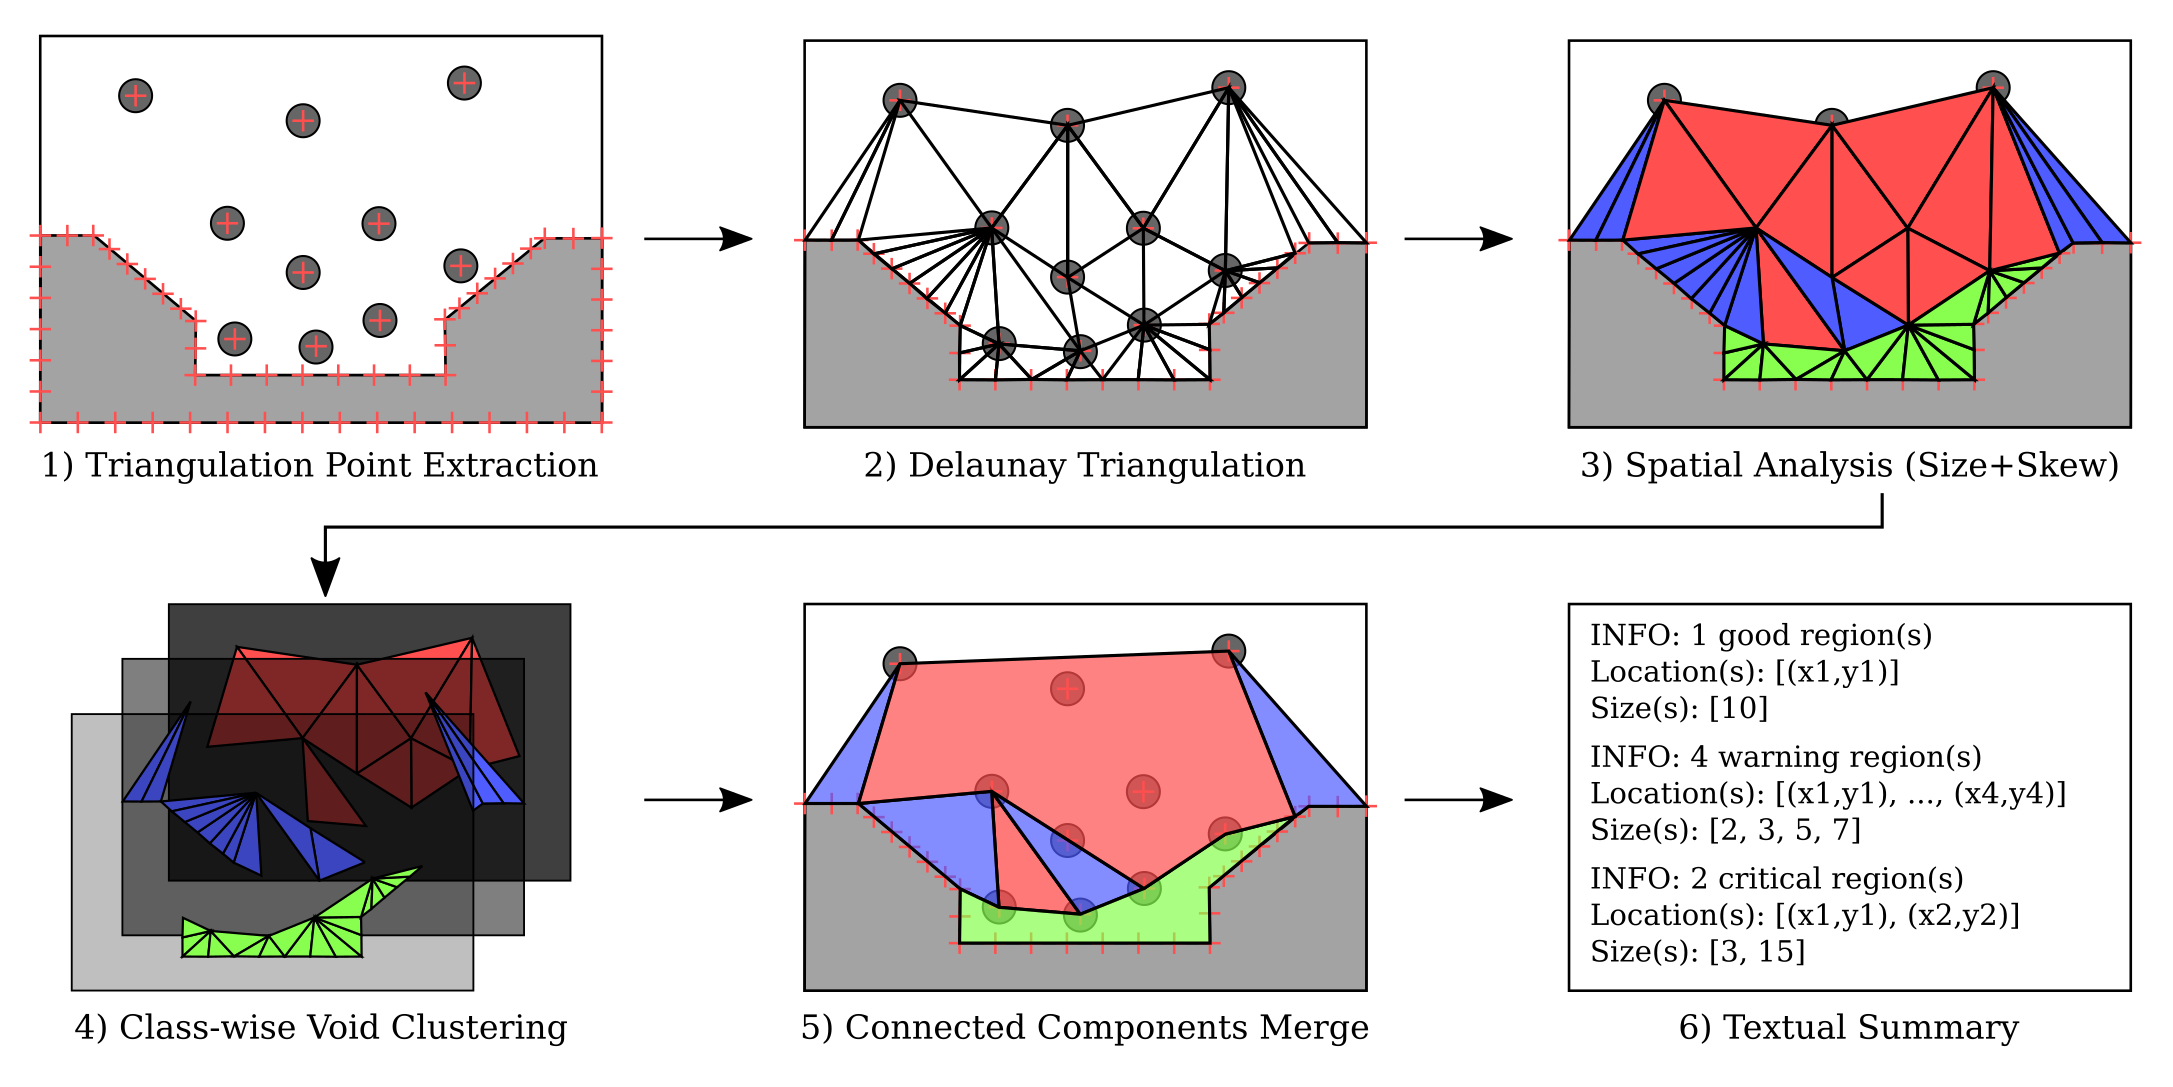
\includegraphics[width=1.035\textwidth]{images/Void_Detection.png}}%
\caption{Diagrammatic overview of toppling risk assessment procedure}
\label{fig:toppling_analysis}
\end{figure}
\vfill

\clearpage
\section{Results and Discussion}
Having completed the experimental phase of the project, a detailed evaluation of the designed pipeline required. This was conducted at both an individual component level (including the detector, tracker, and health analysis components) and combined system level, using appropriate measures to compare the different methods and overall effectiveness. 

\subsection{Detector Performance}
Accuracy and detection speed were the most import measures of performance for the detection algorithms. Detection speed was measured directly as the time to process an image (in milliseconds), with a lower detection time preferred. Average Precision (or AP) was used to score detection accuracy, being the standard metric for object detection tasks, where a higher value is better.

In order to calculate the AP, first the Intersection-Over-Union (IOU) of the detected and ground truth bounding box was computed as follows:
\begin{equation}
    \text{IOU} = \frac{\text{area}(B_p \cap B_{gt})}{\text{area}(B_p \cup B_{gt})}
    \label{eqn:iou}
\end{equation}
where $B_p$ is the predicted bounding box and $B_{gt}$ is the ground truth bounding box. 

The IOU evaluates the level of agreement between the two bounding boxes, and so the detections could then be classified as either true positives (IOU $\geq$ 0.1) or false negatives (IOU $<$ 0.1). A low IOU threshold was used in order to reduce the need for matching bounding box dimensions, given the variability in proposed bounding box shapes for the different methods, and the limited impact this would have on the remainder of the analysis pipeline. The detection results were subsequently sorted by the confidence of the detection algorithm (dynamically computed by the Scaled-YOLOv4 algorithm and statically assigned for the other methods), which were then used to calculate the cumulative precision and recall values, as illustrated by Equations \ref{eqn:prec} and \ref{eqn:rec}.
\begin{equation}
    \text{Precision} = \frac{\text{True Positives}}{\text{True Positives + False Positives}} = \frac{\text{True Positives}}{\text{All Detections}}
    \label{eqn:prec}
\end{equation}
\begin{equation}
    \text{Recall} = \frac{\text{True Positives}}{\text{True Positives + False Negatives}} = \frac{\text{True Positives}}{\text{All Ground Truths}}
    \label{eqn:rec}
\end{equation}

The 11-point average precision \cite{everingham2010pascal} could then be calculated by finding the average precision of the recall at 0.1 intervals between 0 and 1, as shown by:
\begin{equation}
    \text{AP} = \frac{1}{11}\sum_{r\in \{0, 0.1, ..., 1\}} \max_{\tilde{r}:\tilde{r}\geq r} \rho(\tilde{r})
    \label{eqn:ap}
\end{equation}
where $\rho$ is the precision, and $\tilde{r}$ is the (sampled) recall.

Detection speed and accuracy was tested for each method across images with 5, 50, and 500 objects, in order to assess their scalability. The results are presented in Figure \ref{fig:Detector_AP_Time}.

\begin{figure}[h!]
    \begin{center}
	    \resizebox{0.75\textwidth}{!}{
		    %% Creator: Matplotlib, PGF backend
%%
%% To include the figure in your LaTeX document, write
%%   \input{<filename>.pgf}
%%
%% Make sure the required packages are loaded in your preamble
%%   \usepackage{pgf}
%%
%% and, on pdftex
%%   \usepackage[utf8]{inputenc}\DeclareUnicodeCharacter{2212}{-}
%%
%% or, on luatex and xetex
%%   \usepackage{unicode-math}
%%
%% Figures using additional raster images can only be included by \input if
%% they are in the same directory as the main LaTeX file. For loading figures
%% from other directories you can use the `import` package
%%   \usepackage{import}
%%
%% and then include the figures with
%%   \import{<path to file>}{<filename>.pgf}
%%
%% Matplotlib used the following preamble
%%
\begingroup%
\makeatletter%
\begin{pgfpicture}%
\pgfpathrectangle{\pgfpointorigin}{\pgfqpoint{6.000000in}{4.000000in}}%
\pgfusepath{use as bounding box, clip}%
\begin{pgfscope}%
\pgfsetbuttcap%
\pgfsetmiterjoin%
\pgfsetlinewidth{0.000000pt}%
\definecolor{currentstroke}{rgb}{1.000000,1.000000,1.000000}%
\pgfsetstrokecolor{currentstroke}%
\pgfsetstrokeopacity{0.000000}%
\pgfsetdash{}{0pt}%
\pgfpathmoveto{\pgfqpoint{0.000000in}{0.000000in}}%
\pgfpathlineto{\pgfqpoint{6.000000in}{0.000000in}}%
\pgfpathlineto{\pgfqpoint{6.000000in}{4.000000in}}%
\pgfpathlineto{\pgfqpoint{0.000000in}{4.000000in}}%
\pgfpathclose%
\pgfusepath{}%
\end{pgfscope}%
\begin{pgfscope}%
\pgfsetbuttcap%
\pgfsetmiterjoin%
\definecolor{currentfill}{rgb}{1.000000,1.000000,1.000000}%
\pgfsetfillcolor{currentfill}%
\pgfsetlinewidth{0.000000pt}%
\definecolor{currentstroke}{rgb}{0.000000,0.000000,0.000000}%
\pgfsetstrokecolor{currentstroke}%
\pgfsetstrokeopacity{0.000000}%
\pgfsetdash{}{0pt}%
\pgfpathmoveto{\pgfqpoint{0.647292in}{0.605046in}}%
\pgfpathlineto{\pgfqpoint{5.758958in}{0.605046in}}%
\pgfpathlineto{\pgfqpoint{5.758958in}{3.782193in}}%
\pgfpathlineto{\pgfqpoint{0.647292in}{3.782193in}}%
\pgfpathclose%
\pgfusepath{fill}%
\end{pgfscope}%
\begin{pgfscope}%
\pgfsetbuttcap%
\pgfsetroundjoin%
\definecolor{currentfill}{rgb}{0.000000,0.000000,0.000000}%
\pgfsetfillcolor{currentfill}%
\pgfsetlinewidth{0.803000pt}%
\definecolor{currentstroke}{rgb}{0.000000,0.000000,0.000000}%
\pgfsetstrokecolor{currentstroke}%
\pgfsetdash{}{0pt}%
\pgfsys@defobject{currentmarker}{\pgfqpoint{0.000000in}{-0.048611in}}{\pgfqpoint{0.000000in}{0.000000in}}{%
\pgfpathmoveto{\pgfqpoint{0.000000in}{0.000000in}}%
\pgfpathlineto{\pgfqpoint{0.000000in}{-0.048611in}}%
\pgfusepath{stroke,fill}%
}%
\begin{pgfscope}%
\pgfsys@transformshift{0.647292in}{0.605046in}%
\pgfsys@useobject{currentmarker}{}%
\end{pgfscope}%
\end{pgfscope}%
\begin{pgfscope}%
\definecolor{textcolor}{rgb}{0.000000,0.000000,0.000000}%
\pgfsetstrokecolor{textcolor}%
\pgfsetfillcolor{textcolor}%
\pgftext[x=0.647292in,y=0.507824in,,top]{\color{textcolor}\rmfamily\fontsize{11.000000}{13.200000}\selectfont \(\displaystyle {0}\)}%
\end{pgfscope}%
\begin{pgfscope}%
\pgfsetbuttcap%
\pgfsetroundjoin%
\definecolor{currentfill}{rgb}{0.000000,0.000000,0.000000}%
\pgfsetfillcolor{currentfill}%
\pgfsetlinewidth{0.803000pt}%
\definecolor{currentstroke}{rgb}{0.000000,0.000000,0.000000}%
\pgfsetstrokecolor{currentstroke}%
\pgfsetdash{}{0pt}%
\pgfsys@defobject{currentmarker}{\pgfqpoint{0.000000in}{-0.048611in}}{\pgfqpoint{0.000000in}{0.000000in}}{%
\pgfpathmoveto{\pgfqpoint{0.000000in}{0.000000in}}%
\pgfpathlineto{\pgfqpoint{0.000000in}{-0.048611in}}%
\pgfusepath{stroke,fill}%
}%
\begin{pgfscope}%
\pgfsys@transformshift{1.286250in}{0.605046in}%
\pgfsys@useobject{currentmarker}{}%
\end{pgfscope}%
\end{pgfscope}%
\begin{pgfscope}%
\definecolor{textcolor}{rgb}{0.000000,0.000000,0.000000}%
\pgfsetstrokecolor{textcolor}%
\pgfsetfillcolor{textcolor}%
\pgftext[x=1.286250in,y=0.507824in,,top]{\color{textcolor}\rmfamily\fontsize{11.000000}{13.200000}\selectfont \(\displaystyle {10}\)}%
\end{pgfscope}%
\begin{pgfscope}%
\pgfsetbuttcap%
\pgfsetroundjoin%
\definecolor{currentfill}{rgb}{0.000000,0.000000,0.000000}%
\pgfsetfillcolor{currentfill}%
\pgfsetlinewidth{0.803000pt}%
\definecolor{currentstroke}{rgb}{0.000000,0.000000,0.000000}%
\pgfsetstrokecolor{currentstroke}%
\pgfsetdash{}{0pt}%
\pgfsys@defobject{currentmarker}{\pgfqpoint{0.000000in}{-0.048611in}}{\pgfqpoint{0.000000in}{0.000000in}}{%
\pgfpathmoveto{\pgfqpoint{0.000000in}{0.000000in}}%
\pgfpathlineto{\pgfqpoint{0.000000in}{-0.048611in}}%
\pgfusepath{stroke,fill}%
}%
\begin{pgfscope}%
\pgfsys@transformshift{1.925208in}{0.605046in}%
\pgfsys@useobject{currentmarker}{}%
\end{pgfscope}%
\end{pgfscope}%
\begin{pgfscope}%
\definecolor{textcolor}{rgb}{0.000000,0.000000,0.000000}%
\pgfsetstrokecolor{textcolor}%
\pgfsetfillcolor{textcolor}%
\pgftext[x=1.925208in,y=0.507824in,,top]{\color{textcolor}\rmfamily\fontsize{11.000000}{13.200000}\selectfont \(\displaystyle {20}\)}%
\end{pgfscope}%
\begin{pgfscope}%
\pgfsetbuttcap%
\pgfsetroundjoin%
\definecolor{currentfill}{rgb}{0.000000,0.000000,0.000000}%
\pgfsetfillcolor{currentfill}%
\pgfsetlinewidth{0.803000pt}%
\definecolor{currentstroke}{rgb}{0.000000,0.000000,0.000000}%
\pgfsetstrokecolor{currentstroke}%
\pgfsetdash{}{0pt}%
\pgfsys@defobject{currentmarker}{\pgfqpoint{0.000000in}{-0.048611in}}{\pgfqpoint{0.000000in}{0.000000in}}{%
\pgfpathmoveto{\pgfqpoint{0.000000in}{0.000000in}}%
\pgfpathlineto{\pgfqpoint{0.000000in}{-0.048611in}}%
\pgfusepath{stroke,fill}%
}%
\begin{pgfscope}%
\pgfsys@transformshift{2.564167in}{0.605046in}%
\pgfsys@useobject{currentmarker}{}%
\end{pgfscope}%
\end{pgfscope}%
\begin{pgfscope}%
\definecolor{textcolor}{rgb}{0.000000,0.000000,0.000000}%
\pgfsetstrokecolor{textcolor}%
\pgfsetfillcolor{textcolor}%
\pgftext[x=2.564167in,y=0.507824in,,top]{\color{textcolor}\rmfamily\fontsize{11.000000}{13.200000}\selectfont \(\displaystyle {30}\)}%
\end{pgfscope}%
\begin{pgfscope}%
\pgfsetbuttcap%
\pgfsetroundjoin%
\definecolor{currentfill}{rgb}{0.000000,0.000000,0.000000}%
\pgfsetfillcolor{currentfill}%
\pgfsetlinewidth{0.803000pt}%
\definecolor{currentstroke}{rgb}{0.000000,0.000000,0.000000}%
\pgfsetstrokecolor{currentstroke}%
\pgfsetdash{}{0pt}%
\pgfsys@defobject{currentmarker}{\pgfqpoint{0.000000in}{-0.048611in}}{\pgfqpoint{0.000000in}{0.000000in}}{%
\pgfpathmoveto{\pgfqpoint{0.000000in}{0.000000in}}%
\pgfpathlineto{\pgfqpoint{0.000000in}{-0.048611in}}%
\pgfusepath{stroke,fill}%
}%
\begin{pgfscope}%
\pgfsys@transformshift{3.203125in}{0.605046in}%
\pgfsys@useobject{currentmarker}{}%
\end{pgfscope}%
\end{pgfscope}%
\begin{pgfscope}%
\definecolor{textcolor}{rgb}{0.000000,0.000000,0.000000}%
\pgfsetstrokecolor{textcolor}%
\pgfsetfillcolor{textcolor}%
\pgftext[x=3.203125in,y=0.507824in,,top]{\color{textcolor}\rmfamily\fontsize{11.000000}{13.200000}\selectfont \(\displaystyle {40}\)}%
\end{pgfscope}%
\begin{pgfscope}%
\pgfsetbuttcap%
\pgfsetroundjoin%
\definecolor{currentfill}{rgb}{0.000000,0.000000,0.000000}%
\pgfsetfillcolor{currentfill}%
\pgfsetlinewidth{0.803000pt}%
\definecolor{currentstroke}{rgb}{0.000000,0.000000,0.000000}%
\pgfsetstrokecolor{currentstroke}%
\pgfsetdash{}{0pt}%
\pgfsys@defobject{currentmarker}{\pgfqpoint{0.000000in}{-0.048611in}}{\pgfqpoint{0.000000in}{0.000000in}}{%
\pgfpathmoveto{\pgfqpoint{0.000000in}{0.000000in}}%
\pgfpathlineto{\pgfqpoint{0.000000in}{-0.048611in}}%
\pgfusepath{stroke,fill}%
}%
\begin{pgfscope}%
\pgfsys@transformshift{3.842083in}{0.605046in}%
\pgfsys@useobject{currentmarker}{}%
\end{pgfscope}%
\end{pgfscope}%
\begin{pgfscope}%
\definecolor{textcolor}{rgb}{0.000000,0.000000,0.000000}%
\pgfsetstrokecolor{textcolor}%
\pgfsetfillcolor{textcolor}%
\pgftext[x=3.842083in,y=0.507824in,,top]{\color{textcolor}\rmfamily\fontsize{11.000000}{13.200000}\selectfont \(\displaystyle {50}\)}%
\end{pgfscope}%
\begin{pgfscope}%
\pgfsetbuttcap%
\pgfsetroundjoin%
\definecolor{currentfill}{rgb}{0.000000,0.000000,0.000000}%
\pgfsetfillcolor{currentfill}%
\pgfsetlinewidth{0.803000pt}%
\definecolor{currentstroke}{rgb}{0.000000,0.000000,0.000000}%
\pgfsetstrokecolor{currentstroke}%
\pgfsetdash{}{0pt}%
\pgfsys@defobject{currentmarker}{\pgfqpoint{0.000000in}{-0.048611in}}{\pgfqpoint{0.000000in}{0.000000in}}{%
\pgfpathmoveto{\pgfqpoint{0.000000in}{0.000000in}}%
\pgfpathlineto{\pgfqpoint{0.000000in}{-0.048611in}}%
\pgfusepath{stroke,fill}%
}%
\begin{pgfscope}%
\pgfsys@transformshift{4.481042in}{0.605046in}%
\pgfsys@useobject{currentmarker}{}%
\end{pgfscope}%
\end{pgfscope}%
\begin{pgfscope}%
\definecolor{textcolor}{rgb}{0.000000,0.000000,0.000000}%
\pgfsetstrokecolor{textcolor}%
\pgfsetfillcolor{textcolor}%
\pgftext[x=4.481042in,y=0.507824in,,top]{\color{textcolor}\rmfamily\fontsize{11.000000}{13.200000}\selectfont \(\displaystyle {60}\)}%
\end{pgfscope}%
\begin{pgfscope}%
\pgfsetbuttcap%
\pgfsetroundjoin%
\definecolor{currentfill}{rgb}{0.000000,0.000000,0.000000}%
\pgfsetfillcolor{currentfill}%
\pgfsetlinewidth{0.803000pt}%
\definecolor{currentstroke}{rgb}{0.000000,0.000000,0.000000}%
\pgfsetstrokecolor{currentstroke}%
\pgfsetdash{}{0pt}%
\pgfsys@defobject{currentmarker}{\pgfqpoint{0.000000in}{-0.048611in}}{\pgfqpoint{0.000000in}{0.000000in}}{%
\pgfpathmoveto{\pgfqpoint{0.000000in}{0.000000in}}%
\pgfpathlineto{\pgfqpoint{0.000000in}{-0.048611in}}%
\pgfusepath{stroke,fill}%
}%
\begin{pgfscope}%
\pgfsys@transformshift{5.120000in}{0.605046in}%
\pgfsys@useobject{currentmarker}{}%
\end{pgfscope}%
\end{pgfscope}%
\begin{pgfscope}%
\definecolor{textcolor}{rgb}{0.000000,0.000000,0.000000}%
\pgfsetstrokecolor{textcolor}%
\pgfsetfillcolor{textcolor}%
\pgftext[x=5.120000in,y=0.507824in,,top]{\color{textcolor}\rmfamily\fontsize{11.000000}{13.200000}\selectfont \(\displaystyle {70}\)}%
\end{pgfscope}%
\begin{pgfscope}%
\pgfsetbuttcap%
\pgfsetroundjoin%
\definecolor{currentfill}{rgb}{0.000000,0.000000,0.000000}%
\pgfsetfillcolor{currentfill}%
\pgfsetlinewidth{0.803000pt}%
\definecolor{currentstroke}{rgb}{0.000000,0.000000,0.000000}%
\pgfsetstrokecolor{currentstroke}%
\pgfsetdash{}{0pt}%
\pgfsys@defobject{currentmarker}{\pgfqpoint{0.000000in}{-0.048611in}}{\pgfqpoint{0.000000in}{0.000000in}}{%
\pgfpathmoveto{\pgfqpoint{0.000000in}{0.000000in}}%
\pgfpathlineto{\pgfqpoint{0.000000in}{-0.048611in}}%
\pgfusepath{stroke,fill}%
}%
\begin{pgfscope}%
\pgfsys@transformshift{5.758958in}{0.605046in}%
\pgfsys@useobject{currentmarker}{}%
\end{pgfscope}%
\end{pgfscope}%
\begin{pgfscope}%
\definecolor{textcolor}{rgb}{0.000000,0.000000,0.000000}%
\pgfsetstrokecolor{textcolor}%
\pgfsetfillcolor{textcolor}%
\pgftext[x=5.758958in,y=0.507824in,,top]{\color{textcolor}\rmfamily\fontsize{11.000000}{13.200000}\selectfont \(\displaystyle {80}\)}%
\end{pgfscope}%
\begin{pgfscope}%
\definecolor{textcolor}{rgb}{0.000000,0.000000,0.000000}%
\pgfsetstrokecolor{textcolor}%
\pgfsetfillcolor{textcolor}%
\pgftext[x=3.203125in,y=0.317083in,,top]{\color{textcolor}\rmfamily\fontsize{11.000000}{13.200000}\selectfont Detection Speed (ms/image)}%
\end{pgfscope}%
\begin{pgfscope}%
\pgfsetbuttcap%
\pgfsetroundjoin%
\definecolor{currentfill}{rgb}{0.000000,0.000000,0.000000}%
\pgfsetfillcolor{currentfill}%
\pgfsetlinewidth{0.803000pt}%
\definecolor{currentstroke}{rgb}{0.000000,0.000000,0.000000}%
\pgfsetstrokecolor{currentstroke}%
\pgfsetdash{}{0pt}%
\pgfsys@defobject{currentmarker}{\pgfqpoint{-0.048611in}{0.000000in}}{\pgfqpoint{-0.000000in}{0.000000in}}{%
\pgfpathmoveto{\pgfqpoint{-0.000000in}{0.000000in}}%
\pgfpathlineto{\pgfqpoint{-0.048611in}{0.000000in}}%
\pgfusepath{stroke,fill}%
}%
\begin{pgfscope}%
\pgfsys@transformshift{0.647292in}{0.605046in}%
\pgfsys@useobject{currentmarker}{}%
\end{pgfscope}%
\end{pgfscope}%
\begin{pgfscope}%
\definecolor{textcolor}{rgb}{0.000000,0.000000,0.000000}%
\pgfsetstrokecolor{textcolor}%
\pgfsetfillcolor{textcolor}%
\pgftext[x=0.355741in, y=0.552239in, left, base]{\color{textcolor}\rmfamily\fontsize{11.000000}{13.200000}\selectfont \(\displaystyle {0.0}\)}%
\end{pgfscope}%
\begin{pgfscope}%
\pgfsetbuttcap%
\pgfsetroundjoin%
\definecolor{currentfill}{rgb}{0.000000,0.000000,0.000000}%
\pgfsetfillcolor{currentfill}%
\pgfsetlinewidth{0.803000pt}%
\definecolor{currentstroke}{rgb}{0.000000,0.000000,0.000000}%
\pgfsetstrokecolor{currentstroke}%
\pgfsetdash{}{0pt}%
\pgfsys@defobject{currentmarker}{\pgfqpoint{-0.048611in}{0.000000in}}{\pgfqpoint{-0.000000in}{0.000000in}}{%
\pgfpathmoveto{\pgfqpoint{-0.000000in}{0.000000in}}%
\pgfpathlineto{\pgfqpoint{-0.048611in}{0.000000in}}%
\pgfusepath{stroke,fill}%
}%
\begin{pgfscope}%
\pgfsys@transformshift{0.647292in}{1.240476in}%
\pgfsys@useobject{currentmarker}{}%
\end{pgfscope}%
\end{pgfscope}%
\begin{pgfscope}%
\definecolor{textcolor}{rgb}{0.000000,0.000000,0.000000}%
\pgfsetstrokecolor{textcolor}%
\pgfsetfillcolor{textcolor}%
\pgftext[x=0.355741in, y=1.187669in, left, base]{\color{textcolor}\rmfamily\fontsize{11.000000}{13.200000}\selectfont \(\displaystyle {0.2}\)}%
\end{pgfscope}%
\begin{pgfscope}%
\pgfsetbuttcap%
\pgfsetroundjoin%
\definecolor{currentfill}{rgb}{0.000000,0.000000,0.000000}%
\pgfsetfillcolor{currentfill}%
\pgfsetlinewidth{0.803000pt}%
\definecolor{currentstroke}{rgb}{0.000000,0.000000,0.000000}%
\pgfsetstrokecolor{currentstroke}%
\pgfsetdash{}{0pt}%
\pgfsys@defobject{currentmarker}{\pgfqpoint{-0.048611in}{0.000000in}}{\pgfqpoint{-0.000000in}{0.000000in}}{%
\pgfpathmoveto{\pgfqpoint{-0.000000in}{0.000000in}}%
\pgfpathlineto{\pgfqpoint{-0.048611in}{0.000000in}}%
\pgfusepath{stroke,fill}%
}%
\begin{pgfscope}%
\pgfsys@transformshift{0.647292in}{1.875905in}%
\pgfsys@useobject{currentmarker}{}%
\end{pgfscope}%
\end{pgfscope}%
\begin{pgfscope}%
\definecolor{textcolor}{rgb}{0.000000,0.000000,0.000000}%
\pgfsetstrokecolor{textcolor}%
\pgfsetfillcolor{textcolor}%
\pgftext[x=0.355741in, y=1.823098in, left, base]{\color{textcolor}\rmfamily\fontsize{11.000000}{13.200000}\selectfont \(\displaystyle {0.4}\)}%
\end{pgfscope}%
\begin{pgfscope}%
\pgfsetbuttcap%
\pgfsetroundjoin%
\definecolor{currentfill}{rgb}{0.000000,0.000000,0.000000}%
\pgfsetfillcolor{currentfill}%
\pgfsetlinewidth{0.803000pt}%
\definecolor{currentstroke}{rgb}{0.000000,0.000000,0.000000}%
\pgfsetstrokecolor{currentstroke}%
\pgfsetdash{}{0pt}%
\pgfsys@defobject{currentmarker}{\pgfqpoint{-0.048611in}{0.000000in}}{\pgfqpoint{-0.000000in}{0.000000in}}{%
\pgfpathmoveto{\pgfqpoint{-0.000000in}{0.000000in}}%
\pgfpathlineto{\pgfqpoint{-0.048611in}{0.000000in}}%
\pgfusepath{stroke,fill}%
}%
\begin{pgfscope}%
\pgfsys@transformshift{0.647292in}{2.511334in}%
\pgfsys@useobject{currentmarker}{}%
\end{pgfscope}%
\end{pgfscope}%
\begin{pgfscope}%
\definecolor{textcolor}{rgb}{0.000000,0.000000,0.000000}%
\pgfsetstrokecolor{textcolor}%
\pgfsetfillcolor{textcolor}%
\pgftext[x=0.355741in, y=2.458528in, left, base]{\color{textcolor}\rmfamily\fontsize{11.000000}{13.200000}\selectfont \(\displaystyle {0.6}\)}%
\end{pgfscope}%
\begin{pgfscope}%
\pgfsetbuttcap%
\pgfsetroundjoin%
\definecolor{currentfill}{rgb}{0.000000,0.000000,0.000000}%
\pgfsetfillcolor{currentfill}%
\pgfsetlinewidth{0.803000pt}%
\definecolor{currentstroke}{rgb}{0.000000,0.000000,0.000000}%
\pgfsetstrokecolor{currentstroke}%
\pgfsetdash{}{0pt}%
\pgfsys@defobject{currentmarker}{\pgfqpoint{-0.048611in}{0.000000in}}{\pgfqpoint{-0.000000in}{0.000000in}}{%
\pgfpathmoveto{\pgfqpoint{-0.000000in}{0.000000in}}%
\pgfpathlineto{\pgfqpoint{-0.048611in}{0.000000in}}%
\pgfusepath{stroke,fill}%
}%
\begin{pgfscope}%
\pgfsys@transformshift{0.647292in}{3.146764in}%
\pgfsys@useobject{currentmarker}{}%
\end{pgfscope}%
\end{pgfscope}%
\begin{pgfscope}%
\definecolor{textcolor}{rgb}{0.000000,0.000000,0.000000}%
\pgfsetstrokecolor{textcolor}%
\pgfsetfillcolor{textcolor}%
\pgftext[x=0.355741in, y=3.093957in, left, base]{\color{textcolor}\rmfamily\fontsize{11.000000}{13.200000}\selectfont \(\displaystyle {0.8}\)}%
\end{pgfscope}%
\begin{pgfscope}%
\pgfsetbuttcap%
\pgfsetroundjoin%
\definecolor{currentfill}{rgb}{0.000000,0.000000,0.000000}%
\pgfsetfillcolor{currentfill}%
\pgfsetlinewidth{0.803000pt}%
\definecolor{currentstroke}{rgb}{0.000000,0.000000,0.000000}%
\pgfsetstrokecolor{currentstroke}%
\pgfsetdash{}{0pt}%
\pgfsys@defobject{currentmarker}{\pgfqpoint{-0.048611in}{0.000000in}}{\pgfqpoint{-0.000000in}{0.000000in}}{%
\pgfpathmoveto{\pgfqpoint{-0.000000in}{0.000000in}}%
\pgfpathlineto{\pgfqpoint{-0.048611in}{0.000000in}}%
\pgfusepath{stroke,fill}%
}%
\begin{pgfscope}%
\pgfsys@transformshift{0.647292in}{3.782193in}%
\pgfsys@useobject{currentmarker}{}%
\end{pgfscope}%
\end{pgfscope}%
\begin{pgfscope}%
\definecolor{textcolor}{rgb}{0.000000,0.000000,0.000000}%
\pgfsetstrokecolor{textcolor}%
\pgfsetfillcolor{textcolor}%
\pgftext[x=0.355741in, y=3.729387in, left, base]{\color{textcolor}\rmfamily\fontsize{11.000000}{13.200000}\selectfont \(\displaystyle {1.0}\)}%
\end{pgfscope}%
\begin{pgfscope}%
\definecolor{textcolor}{rgb}{0.000000,0.000000,0.000000}%
\pgfsetstrokecolor{textcolor}%
\pgfsetfillcolor{textcolor}%
\pgftext[x=0.300185in,y=2.193620in,,bottom,rotate=90.000000]{\color{textcolor}\rmfamily\fontsize{11.000000}{13.200000}\selectfont Test AP}%
\end{pgfscope}%
\begin{pgfscope}%
\pgfpathrectangle{\pgfqpoint{0.647292in}{0.605046in}}{\pgfqpoint{5.111666in}{3.177147in}}%
\pgfusepath{clip}%
\pgfsetrectcap%
\pgfsetroundjoin%
\pgfsetlinewidth{1.505625pt}%
\definecolor{currentstroke}{rgb}{0.121569,0.466667,0.705882}%
\pgfsetstrokecolor{currentstroke}%
\pgfsetdash{}{0pt}%
\pgfpathmoveto{\pgfqpoint{0.807531in}{1.944898in}}%
\pgfpathlineto{\pgfqpoint{0.901058in}{2.005746in}}%
\pgfpathlineto{\pgfqpoint{1.382821in}{2.583312in}}%
\pgfusepath{stroke}%
\end{pgfscope}%
\begin{pgfscope}%
\pgfpathrectangle{\pgfqpoint{0.647292in}{0.605046in}}{\pgfqpoint{5.111666in}{3.177147in}}%
\pgfusepath{clip}%
\pgfsetbuttcap%
\pgfsetroundjoin%
\definecolor{currentfill}{rgb}{0.000000,0.000000,0.000000}%
\pgfsetfillcolor{currentfill}%
\pgfsetfillopacity{0.000000}%
\pgfsetlinewidth{1.003750pt}%
\definecolor{currentstroke}{rgb}{0.121569,0.466667,0.705882}%
\pgfsetstrokecolor{currentstroke}%
\pgfsetdash{}{0pt}%
\pgfsys@defobject{currentmarker}{\pgfqpoint{-0.041667in}{-0.041667in}}{\pgfqpoint{0.041667in}{0.041667in}}{%
\pgfpathmoveto{\pgfqpoint{0.000000in}{-0.041667in}}%
\pgfpathcurveto{\pgfqpoint{0.011050in}{-0.041667in}}{\pgfqpoint{0.021649in}{-0.037276in}}{\pgfqpoint{0.029463in}{-0.029463in}}%
\pgfpathcurveto{\pgfqpoint{0.037276in}{-0.021649in}}{\pgfqpoint{0.041667in}{-0.011050in}}{\pgfqpoint{0.041667in}{0.000000in}}%
\pgfpathcurveto{\pgfqpoint{0.041667in}{0.011050in}}{\pgfqpoint{0.037276in}{0.021649in}}{\pgfqpoint{0.029463in}{0.029463in}}%
\pgfpathcurveto{\pgfqpoint{0.021649in}{0.037276in}}{\pgfqpoint{0.011050in}{0.041667in}}{\pgfqpoint{0.000000in}{0.041667in}}%
\pgfpathcurveto{\pgfqpoint{-0.011050in}{0.041667in}}{\pgfqpoint{-0.021649in}{0.037276in}}{\pgfqpoint{-0.029463in}{0.029463in}}%
\pgfpathcurveto{\pgfqpoint{-0.037276in}{0.021649in}}{\pgfqpoint{-0.041667in}{0.011050in}}{\pgfqpoint{-0.041667in}{0.000000in}}%
\pgfpathcurveto{\pgfqpoint{-0.041667in}{-0.011050in}}{\pgfqpoint{-0.037276in}{-0.021649in}}{\pgfqpoint{-0.029463in}{-0.029463in}}%
\pgfpathcurveto{\pgfqpoint{-0.021649in}{-0.037276in}}{\pgfqpoint{-0.011050in}{-0.041667in}}{\pgfqpoint{0.000000in}{-0.041667in}}%
\pgfpathclose%
\pgfusepath{stroke,fill}%
}%
\begin{pgfscope}%
\pgfsys@transformshift{0.807531in}{1.944898in}%
\pgfsys@useobject{currentmarker}{}%
\end{pgfscope}%
\end{pgfscope}%
\begin{pgfscope}%
\pgfpathrectangle{\pgfqpoint{0.647292in}{0.605046in}}{\pgfqpoint{5.111666in}{3.177147in}}%
\pgfusepath{clip}%
\pgfsetbuttcap%
\pgfsetmiterjoin%
\definecolor{currentfill}{rgb}{0.000000,0.000000,0.000000}%
\pgfsetfillcolor{currentfill}%
\pgfsetfillopacity{0.000000}%
\pgfsetlinewidth{1.003750pt}%
\definecolor{currentstroke}{rgb}{0.121569,0.466667,0.705882}%
\pgfsetstrokecolor{currentstroke}%
\pgfsetdash{}{0pt}%
\pgfsys@defobject{currentmarker}{\pgfqpoint{-0.041667in}{-0.041667in}}{\pgfqpoint{0.041667in}{0.041667in}}{%
\pgfpathmoveto{\pgfqpoint{-0.041667in}{-0.041667in}}%
\pgfpathlineto{\pgfqpoint{0.041667in}{-0.041667in}}%
\pgfpathlineto{\pgfqpoint{0.041667in}{0.041667in}}%
\pgfpathlineto{\pgfqpoint{-0.041667in}{0.041667in}}%
\pgfpathclose%
\pgfusepath{stroke,fill}%
}%
\begin{pgfscope}%
\pgfsys@transformshift{0.901058in}{2.005746in}%
\pgfsys@useobject{currentmarker}{}%
\end{pgfscope}%
\end{pgfscope}%
\begin{pgfscope}%
\pgfpathrectangle{\pgfqpoint{0.647292in}{0.605046in}}{\pgfqpoint{5.111666in}{3.177147in}}%
\pgfusepath{clip}%
\pgfsetbuttcap%
\pgfsetmiterjoin%
\definecolor{currentfill}{rgb}{0.000000,0.000000,0.000000}%
\pgfsetfillcolor{currentfill}%
\pgfsetfillopacity{0.000000}%
\pgfsetlinewidth{1.003750pt}%
\definecolor{currentstroke}{rgb}{0.121569,0.466667,0.705882}%
\pgfsetstrokecolor{currentstroke}%
\pgfsetdash{}{0pt}%
\pgfsys@defobject{currentmarker}{\pgfqpoint{-0.041667in}{-0.041667in}}{\pgfqpoint{0.041667in}{0.041667in}}{%
\pgfpathmoveto{\pgfqpoint{-0.000000in}{-0.041667in}}%
\pgfpathlineto{\pgfqpoint{0.041667in}{0.041667in}}%
\pgfpathlineto{\pgfqpoint{-0.041667in}{0.041667in}}%
\pgfpathclose%
\pgfusepath{stroke,fill}%
}%
\begin{pgfscope}%
\pgfsys@transformshift{1.382821in}{2.583312in}%
\pgfsys@useobject{currentmarker}{}%
\end{pgfscope}%
\end{pgfscope}%
\begin{pgfscope}%
\pgfpathrectangle{\pgfqpoint{0.647292in}{0.605046in}}{\pgfqpoint{5.111666in}{3.177147in}}%
\pgfusepath{clip}%
\pgfsetrectcap%
\pgfsetroundjoin%
\pgfsetlinewidth{1.505625pt}%
\definecolor{currentstroke}{rgb}{1.000000,0.498039,0.054902}%
\pgfsetstrokecolor{currentstroke}%
\pgfsetdash{}{0pt}%
\pgfpathmoveto{\pgfqpoint{1.138881in}{0.946237in}}%
\pgfpathlineto{\pgfqpoint{1.203172in}{0.903245in}}%
\pgfpathlineto{\pgfqpoint{1.515444in}{0.677254in}}%
\pgfusepath{stroke}%
\end{pgfscope}%
\begin{pgfscope}%
\pgfpathrectangle{\pgfqpoint{0.647292in}{0.605046in}}{\pgfqpoint{5.111666in}{3.177147in}}%
\pgfusepath{clip}%
\pgfsetbuttcap%
\pgfsetroundjoin%
\definecolor{currentfill}{rgb}{0.000000,0.000000,0.000000}%
\pgfsetfillcolor{currentfill}%
\pgfsetfillopacity{0.000000}%
\pgfsetlinewidth{1.003750pt}%
\definecolor{currentstroke}{rgb}{1.000000,0.498039,0.054902}%
\pgfsetstrokecolor{currentstroke}%
\pgfsetdash{}{0pt}%
\pgfsys@defobject{currentmarker}{\pgfqpoint{-0.041667in}{-0.041667in}}{\pgfqpoint{0.041667in}{0.041667in}}{%
\pgfpathmoveto{\pgfqpoint{0.000000in}{-0.041667in}}%
\pgfpathcurveto{\pgfqpoint{0.011050in}{-0.041667in}}{\pgfqpoint{0.021649in}{-0.037276in}}{\pgfqpoint{0.029463in}{-0.029463in}}%
\pgfpathcurveto{\pgfqpoint{0.037276in}{-0.021649in}}{\pgfqpoint{0.041667in}{-0.011050in}}{\pgfqpoint{0.041667in}{0.000000in}}%
\pgfpathcurveto{\pgfqpoint{0.041667in}{0.011050in}}{\pgfqpoint{0.037276in}{0.021649in}}{\pgfqpoint{0.029463in}{0.029463in}}%
\pgfpathcurveto{\pgfqpoint{0.021649in}{0.037276in}}{\pgfqpoint{0.011050in}{0.041667in}}{\pgfqpoint{0.000000in}{0.041667in}}%
\pgfpathcurveto{\pgfqpoint{-0.011050in}{0.041667in}}{\pgfqpoint{-0.021649in}{0.037276in}}{\pgfqpoint{-0.029463in}{0.029463in}}%
\pgfpathcurveto{\pgfqpoint{-0.037276in}{0.021649in}}{\pgfqpoint{-0.041667in}{0.011050in}}{\pgfqpoint{-0.041667in}{0.000000in}}%
\pgfpathcurveto{\pgfqpoint{-0.041667in}{-0.011050in}}{\pgfqpoint{-0.037276in}{-0.021649in}}{\pgfqpoint{-0.029463in}{-0.029463in}}%
\pgfpathcurveto{\pgfqpoint{-0.021649in}{-0.037276in}}{\pgfqpoint{-0.011050in}{-0.041667in}}{\pgfqpoint{0.000000in}{-0.041667in}}%
\pgfpathclose%
\pgfusepath{stroke,fill}%
}%
\begin{pgfscope}%
\pgfsys@transformshift{1.138881in}{0.946237in}%
\pgfsys@useobject{currentmarker}{}%
\end{pgfscope}%
\end{pgfscope}%
\begin{pgfscope}%
\pgfpathrectangle{\pgfqpoint{0.647292in}{0.605046in}}{\pgfqpoint{5.111666in}{3.177147in}}%
\pgfusepath{clip}%
\pgfsetbuttcap%
\pgfsetmiterjoin%
\definecolor{currentfill}{rgb}{0.000000,0.000000,0.000000}%
\pgfsetfillcolor{currentfill}%
\pgfsetfillopacity{0.000000}%
\pgfsetlinewidth{1.003750pt}%
\definecolor{currentstroke}{rgb}{1.000000,0.498039,0.054902}%
\pgfsetstrokecolor{currentstroke}%
\pgfsetdash{}{0pt}%
\pgfsys@defobject{currentmarker}{\pgfqpoint{-0.041667in}{-0.041667in}}{\pgfqpoint{0.041667in}{0.041667in}}{%
\pgfpathmoveto{\pgfqpoint{-0.041667in}{-0.041667in}}%
\pgfpathlineto{\pgfqpoint{0.041667in}{-0.041667in}}%
\pgfpathlineto{\pgfqpoint{0.041667in}{0.041667in}}%
\pgfpathlineto{\pgfqpoint{-0.041667in}{0.041667in}}%
\pgfpathclose%
\pgfusepath{stroke,fill}%
}%
\begin{pgfscope}%
\pgfsys@transformshift{1.203172in}{0.903245in}%
\pgfsys@useobject{currentmarker}{}%
\end{pgfscope}%
\end{pgfscope}%
\begin{pgfscope}%
\pgfpathrectangle{\pgfqpoint{0.647292in}{0.605046in}}{\pgfqpoint{5.111666in}{3.177147in}}%
\pgfusepath{clip}%
\pgfsetbuttcap%
\pgfsetmiterjoin%
\definecolor{currentfill}{rgb}{0.000000,0.000000,0.000000}%
\pgfsetfillcolor{currentfill}%
\pgfsetfillopacity{0.000000}%
\pgfsetlinewidth{1.003750pt}%
\definecolor{currentstroke}{rgb}{1.000000,0.498039,0.054902}%
\pgfsetstrokecolor{currentstroke}%
\pgfsetdash{}{0pt}%
\pgfsys@defobject{currentmarker}{\pgfqpoint{-0.041667in}{-0.041667in}}{\pgfqpoint{0.041667in}{0.041667in}}{%
\pgfpathmoveto{\pgfqpoint{-0.000000in}{-0.041667in}}%
\pgfpathlineto{\pgfqpoint{0.041667in}{0.041667in}}%
\pgfpathlineto{\pgfqpoint{-0.041667in}{0.041667in}}%
\pgfpathclose%
\pgfusepath{stroke,fill}%
}%
\begin{pgfscope}%
\pgfsys@transformshift{1.515444in}{0.677254in}%
\pgfsys@useobject{currentmarker}{}%
\end{pgfscope}%
\end{pgfscope}%
\begin{pgfscope}%
\pgfpathrectangle{\pgfqpoint{0.647292in}{0.605046in}}{\pgfqpoint{5.111666in}{3.177147in}}%
\pgfusepath{clip}%
\pgfsetrectcap%
\pgfsetroundjoin%
\pgfsetlinewidth{1.505625pt}%
\definecolor{currentstroke}{rgb}{0.172549,0.627451,0.172549}%
\pgfsetstrokecolor{currentstroke}%
\pgfsetdash{}{0pt}%
\pgfpathmoveto{\pgfqpoint{2.750990in}{3.493362in}}%
\pgfpathlineto{\pgfqpoint{2.894219in}{3.203907in}}%
\pgfpathlineto{\pgfqpoint{3.954295in}{3.185103in}}%
\pgfusepath{stroke}%
\end{pgfscope}%
\begin{pgfscope}%
\pgfpathrectangle{\pgfqpoint{0.647292in}{0.605046in}}{\pgfqpoint{5.111666in}{3.177147in}}%
\pgfusepath{clip}%
\pgfsetbuttcap%
\pgfsetroundjoin%
\definecolor{currentfill}{rgb}{0.000000,0.000000,0.000000}%
\pgfsetfillcolor{currentfill}%
\pgfsetfillopacity{0.000000}%
\pgfsetlinewidth{1.003750pt}%
\definecolor{currentstroke}{rgb}{0.172549,0.627451,0.172549}%
\pgfsetstrokecolor{currentstroke}%
\pgfsetdash{}{0pt}%
\pgfsys@defobject{currentmarker}{\pgfqpoint{-0.041667in}{-0.041667in}}{\pgfqpoint{0.041667in}{0.041667in}}{%
\pgfpathmoveto{\pgfqpoint{0.000000in}{-0.041667in}}%
\pgfpathcurveto{\pgfqpoint{0.011050in}{-0.041667in}}{\pgfqpoint{0.021649in}{-0.037276in}}{\pgfqpoint{0.029463in}{-0.029463in}}%
\pgfpathcurveto{\pgfqpoint{0.037276in}{-0.021649in}}{\pgfqpoint{0.041667in}{-0.011050in}}{\pgfqpoint{0.041667in}{0.000000in}}%
\pgfpathcurveto{\pgfqpoint{0.041667in}{0.011050in}}{\pgfqpoint{0.037276in}{0.021649in}}{\pgfqpoint{0.029463in}{0.029463in}}%
\pgfpathcurveto{\pgfqpoint{0.021649in}{0.037276in}}{\pgfqpoint{0.011050in}{0.041667in}}{\pgfqpoint{0.000000in}{0.041667in}}%
\pgfpathcurveto{\pgfqpoint{-0.011050in}{0.041667in}}{\pgfqpoint{-0.021649in}{0.037276in}}{\pgfqpoint{-0.029463in}{0.029463in}}%
\pgfpathcurveto{\pgfqpoint{-0.037276in}{0.021649in}}{\pgfqpoint{-0.041667in}{0.011050in}}{\pgfqpoint{-0.041667in}{0.000000in}}%
\pgfpathcurveto{\pgfqpoint{-0.041667in}{-0.011050in}}{\pgfqpoint{-0.037276in}{-0.021649in}}{\pgfqpoint{-0.029463in}{-0.029463in}}%
\pgfpathcurveto{\pgfqpoint{-0.021649in}{-0.037276in}}{\pgfqpoint{-0.011050in}{-0.041667in}}{\pgfqpoint{0.000000in}{-0.041667in}}%
\pgfpathclose%
\pgfusepath{stroke,fill}%
}%
\begin{pgfscope}%
\pgfsys@transformshift{2.750990in}{3.493362in}%
\pgfsys@useobject{currentmarker}{}%
\end{pgfscope}%
\end{pgfscope}%
\begin{pgfscope}%
\pgfpathrectangle{\pgfqpoint{0.647292in}{0.605046in}}{\pgfqpoint{5.111666in}{3.177147in}}%
\pgfusepath{clip}%
\pgfsetbuttcap%
\pgfsetmiterjoin%
\definecolor{currentfill}{rgb}{0.000000,0.000000,0.000000}%
\pgfsetfillcolor{currentfill}%
\pgfsetfillopacity{0.000000}%
\pgfsetlinewidth{1.003750pt}%
\definecolor{currentstroke}{rgb}{0.172549,0.627451,0.172549}%
\pgfsetstrokecolor{currentstroke}%
\pgfsetdash{}{0pt}%
\pgfsys@defobject{currentmarker}{\pgfqpoint{-0.041667in}{-0.041667in}}{\pgfqpoint{0.041667in}{0.041667in}}{%
\pgfpathmoveto{\pgfqpoint{-0.041667in}{-0.041667in}}%
\pgfpathlineto{\pgfqpoint{0.041667in}{-0.041667in}}%
\pgfpathlineto{\pgfqpoint{0.041667in}{0.041667in}}%
\pgfpathlineto{\pgfqpoint{-0.041667in}{0.041667in}}%
\pgfpathclose%
\pgfusepath{stroke,fill}%
}%
\begin{pgfscope}%
\pgfsys@transformshift{2.894219in}{3.203907in}%
\pgfsys@useobject{currentmarker}{}%
\end{pgfscope}%
\end{pgfscope}%
\begin{pgfscope}%
\pgfpathrectangle{\pgfqpoint{0.647292in}{0.605046in}}{\pgfqpoint{5.111666in}{3.177147in}}%
\pgfusepath{clip}%
\pgfsetbuttcap%
\pgfsetmiterjoin%
\definecolor{currentfill}{rgb}{0.000000,0.000000,0.000000}%
\pgfsetfillcolor{currentfill}%
\pgfsetfillopacity{0.000000}%
\pgfsetlinewidth{1.003750pt}%
\definecolor{currentstroke}{rgb}{0.172549,0.627451,0.172549}%
\pgfsetstrokecolor{currentstroke}%
\pgfsetdash{}{0pt}%
\pgfsys@defobject{currentmarker}{\pgfqpoint{-0.041667in}{-0.041667in}}{\pgfqpoint{0.041667in}{0.041667in}}{%
\pgfpathmoveto{\pgfqpoint{-0.000000in}{-0.041667in}}%
\pgfpathlineto{\pgfqpoint{0.041667in}{0.041667in}}%
\pgfpathlineto{\pgfqpoint{-0.041667in}{0.041667in}}%
\pgfpathclose%
\pgfusepath{stroke,fill}%
}%
\begin{pgfscope}%
\pgfsys@transformshift{3.954295in}{3.185103in}%
\pgfsys@useobject{currentmarker}{}%
\end{pgfscope}%
\end{pgfscope}%
\begin{pgfscope}%
\pgfpathrectangle{\pgfqpoint{0.647292in}{0.605046in}}{\pgfqpoint{5.111666in}{3.177147in}}%
\pgfusepath{clip}%
\pgfsetrectcap%
\pgfsetroundjoin%
\pgfsetlinewidth{1.505625pt}%
\definecolor{currentstroke}{rgb}{0.839216,0.152941,0.156863}%
\pgfsetstrokecolor{currentstroke}%
\pgfsetdash{}{0pt}%
\pgfpathmoveto{\pgfqpoint{2.757859in}{3.234041in}}%
\pgfpathlineto{\pgfqpoint{2.950484in}{2.942913in}}%
\pgfpathlineto{\pgfqpoint{4.946440in}{2.960624in}}%
\pgfusepath{stroke}%
\end{pgfscope}%
\begin{pgfscope}%
\pgfpathrectangle{\pgfqpoint{0.647292in}{0.605046in}}{\pgfqpoint{5.111666in}{3.177147in}}%
\pgfusepath{clip}%
\pgfsetbuttcap%
\pgfsetroundjoin%
\definecolor{currentfill}{rgb}{0.000000,0.000000,0.000000}%
\pgfsetfillcolor{currentfill}%
\pgfsetfillopacity{0.000000}%
\pgfsetlinewidth{1.003750pt}%
\definecolor{currentstroke}{rgb}{0.839216,0.152941,0.156863}%
\pgfsetstrokecolor{currentstroke}%
\pgfsetdash{}{0pt}%
\pgfsys@defobject{currentmarker}{\pgfqpoint{-0.041667in}{-0.041667in}}{\pgfqpoint{0.041667in}{0.041667in}}{%
\pgfpathmoveto{\pgfqpoint{0.000000in}{-0.041667in}}%
\pgfpathcurveto{\pgfqpoint{0.011050in}{-0.041667in}}{\pgfqpoint{0.021649in}{-0.037276in}}{\pgfqpoint{0.029463in}{-0.029463in}}%
\pgfpathcurveto{\pgfqpoint{0.037276in}{-0.021649in}}{\pgfqpoint{0.041667in}{-0.011050in}}{\pgfqpoint{0.041667in}{0.000000in}}%
\pgfpathcurveto{\pgfqpoint{0.041667in}{0.011050in}}{\pgfqpoint{0.037276in}{0.021649in}}{\pgfqpoint{0.029463in}{0.029463in}}%
\pgfpathcurveto{\pgfqpoint{0.021649in}{0.037276in}}{\pgfqpoint{0.011050in}{0.041667in}}{\pgfqpoint{0.000000in}{0.041667in}}%
\pgfpathcurveto{\pgfqpoint{-0.011050in}{0.041667in}}{\pgfqpoint{-0.021649in}{0.037276in}}{\pgfqpoint{-0.029463in}{0.029463in}}%
\pgfpathcurveto{\pgfqpoint{-0.037276in}{0.021649in}}{\pgfqpoint{-0.041667in}{0.011050in}}{\pgfqpoint{-0.041667in}{0.000000in}}%
\pgfpathcurveto{\pgfqpoint{-0.041667in}{-0.011050in}}{\pgfqpoint{-0.037276in}{-0.021649in}}{\pgfqpoint{-0.029463in}{-0.029463in}}%
\pgfpathcurveto{\pgfqpoint{-0.021649in}{-0.037276in}}{\pgfqpoint{-0.011050in}{-0.041667in}}{\pgfqpoint{0.000000in}{-0.041667in}}%
\pgfpathclose%
\pgfusepath{stroke,fill}%
}%
\begin{pgfscope}%
\pgfsys@transformshift{2.757859in}{3.234041in}%
\pgfsys@useobject{currentmarker}{}%
\end{pgfscope}%
\end{pgfscope}%
\begin{pgfscope}%
\pgfpathrectangle{\pgfqpoint{0.647292in}{0.605046in}}{\pgfqpoint{5.111666in}{3.177147in}}%
\pgfusepath{clip}%
\pgfsetbuttcap%
\pgfsetmiterjoin%
\definecolor{currentfill}{rgb}{0.000000,0.000000,0.000000}%
\pgfsetfillcolor{currentfill}%
\pgfsetfillopacity{0.000000}%
\pgfsetlinewidth{1.003750pt}%
\definecolor{currentstroke}{rgb}{0.839216,0.152941,0.156863}%
\pgfsetstrokecolor{currentstroke}%
\pgfsetdash{}{0pt}%
\pgfsys@defobject{currentmarker}{\pgfqpoint{-0.041667in}{-0.041667in}}{\pgfqpoint{0.041667in}{0.041667in}}{%
\pgfpathmoveto{\pgfqpoint{-0.041667in}{-0.041667in}}%
\pgfpathlineto{\pgfqpoint{0.041667in}{-0.041667in}}%
\pgfpathlineto{\pgfqpoint{0.041667in}{0.041667in}}%
\pgfpathlineto{\pgfqpoint{-0.041667in}{0.041667in}}%
\pgfpathclose%
\pgfusepath{stroke,fill}%
}%
\begin{pgfscope}%
\pgfsys@transformshift{2.950484in}{2.942913in}%
\pgfsys@useobject{currentmarker}{}%
\end{pgfscope}%
\end{pgfscope}%
\begin{pgfscope}%
\pgfpathrectangle{\pgfqpoint{0.647292in}{0.605046in}}{\pgfqpoint{5.111666in}{3.177147in}}%
\pgfusepath{clip}%
\pgfsetbuttcap%
\pgfsetmiterjoin%
\definecolor{currentfill}{rgb}{0.000000,0.000000,0.000000}%
\pgfsetfillcolor{currentfill}%
\pgfsetfillopacity{0.000000}%
\pgfsetlinewidth{1.003750pt}%
\definecolor{currentstroke}{rgb}{0.839216,0.152941,0.156863}%
\pgfsetstrokecolor{currentstroke}%
\pgfsetdash{}{0pt}%
\pgfsys@defobject{currentmarker}{\pgfqpoint{-0.041667in}{-0.041667in}}{\pgfqpoint{0.041667in}{0.041667in}}{%
\pgfpathmoveto{\pgfqpoint{-0.000000in}{-0.041667in}}%
\pgfpathlineto{\pgfqpoint{0.041667in}{0.041667in}}%
\pgfpathlineto{\pgfqpoint{-0.041667in}{0.041667in}}%
\pgfpathclose%
\pgfusepath{stroke,fill}%
}%
\begin{pgfscope}%
\pgfsys@transformshift{4.946440in}{2.960624in}%
\pgfsys@useobject{currentmarker}{}%
\end{pgfscope}%
\end{pgfscope}%
\begin{pgfscope}%
\pgfpathrectangle{\pgfqpoint{0.647292in}{0.605046in}}{\pgfqpoint{5.111666in}{3.177147in}}%
\pgfusepath{clip}%
\pgfsetrectcap%
\pgfsetroundjoin%
\pgfsetlinewidth{1.505625pt}%
\definecolor{currentstroke}{rgb}{0.580392,0.403922,0.741176}%
\pgfsetstrokecolor{currentstroke}%
\pgfsetdash{}{0pt}%
\pgfpathmoveto{\pgfqpoint{2.029446in}{3.493362in}}%
\pgfpathlineto{\pgfqpoint{2.116985in}{3.493362in}}%
\pgfpathlineto{\pgfqpoint{2.659695in}{3.493362in}}%
\pgfusepath{stroke}%
\end{pgfscope}%
\begin{pgfscope}%
\pgfpathrectangle{\pgfqpoint{0.647292in}{0.605046in}}{\pgfqpoint{5.111666in}{3.177147in}}%
\pgfusepath{clip}%
\pgfsetbuttcap%
\pgfsetroundjoin%
\definecolor{currentfill}{rgb}{0.000000,0.000000,0.000000}%
\pgfsetfillcolor{currentfill}%
\pgfsetfillopacity{0.000000}%
\pgfsetlinewidth{1.003750pt}%
\definecolor{currentstroke}{rgb}{0.580392,0.403922,0.741176}%
\pgfsetstrokecolor{currentstroke}%
\pgfsetdash{}{0pt}%
\pgfsys@defobject{currentmarker}{\pgfqpoint{-0.041667in}{-0.041667in}}{\pgfqpoint{0.041667in}{0.041667in}}{%
\pgfpathmoveto{\pgfqpoint{0.000000in}{-0.041667in}}%
\pgfpathcurveto{\pgfqpoint{0.011050in}{-0.041667in}}{\pgfqpoint{0.021649in}{-0.037276in}}{\pgfqpoint{0.029463in}{-0.029463in}}%
\pgfpathcurveto{\pgfqpoint{0.037276in}{-0.021649in}}{\pgfqpoint{0.041667in}{-0.011050in}}{\pgfqpoint{0.041667in}{0.000000in}}%
\pgfpathcurveto{\pgfqpoint{0.041667in}{0.011050in}}{\pgfqpoint{0.037276in}{0.021649in}}{\pgfqpoint{0.029463in}{0.029463in}}%
\pgfpathcurveto{\pgfqpoint{0.021649in}{0.037276in}}{\pgfqpoint{0.011050in}{0.041667in}}{\pgfqpoint{0.000000in}{0.041667in}}%
\pgfpathcurveto{\pgfqpoint{-0.011050in}{0.041667in}}{\pgfqpoint{-0.021649in}{0.037276in}}{\pgfqpoint{-0.029463in}{0.029463in}}%
\pgfpathcurveto{\pgfqpoint{-0.037276in}{0.021649in}}{\pgfqpoint{-0.041667in}{0.011050in}}{\pgfqpoint{-0.041667in}{0.000000in}}%
\pgfpathcurveto{\pgfqpoint{-0.041667in}{-0.011050in}}{\pgfqpoint{-0.037276in}{-0.021649in}}{\pgfqpoint{-0.029463in}{-0.029463in}}%
\pgfpathcurveto{\pgfqpoint{-0.021649in}{-0.037276in}}{\pgfqpoint{-0.011050in}{-0.041667in}}{\pgfqpoint{0.000000in}{-0.041667in}}%
\pgfpathclose%
\pgfusepath{stroke,fill}%
}%
\begin{pgfscope}%
\pgfsys@transformshift{2.029446in}{3.493362in}%
\pgfsys@useobject{currentmarker}{}%
\end{pgfscope}%
\end{pgfscope}%
\begin{pgfscope}%
\pgfpathrectangle{\pgfqpoint{0.647292in}{0.605046in}}{\pgfqpoint{5.111666in}{3.177147in}}%
\pgfusepath{clip}%
\pgfsetbuttcap%
\pgfsetmiterjoin%
\definecolor{currentfill}{rgb}{0.000000,0.000000,0.000000}%
\pgfsetfillcolor{currentfill}%
\pgfsetfillopacity{0.000000}%
\pgfsetlinewidth{1.003750pt}%
\definecolor{currentstroke}{rgb}{0.580392,0.403922,0.741176}%
\pgfsetstrokecolor{currentstroke}%
\pgfsetdash{}{0pt}%
\pgfsys@defobject{currentmarker}{\pgfqpoint{-0.041667in}{-0.041667in}}{\pgfqpoint{0.041667in}{0.041667in}}{%
\pgfpathmoveto{\pgfqpoint{-0.041667in}{-0.041667in}}%
\pgfpathlineto{\pgfqpoint{0.041667in}{-0.041667in}}%
\pgfpathlineto{\pgfqpoint{0.041667in}{0.041667in}}%
\pgfpathlineto{\pgfqpoint{-0.041667in}{0.041667in}}%
\pgfpathclose%
\pgfusepath{stroke,fill}%
}%
\begin{pgfscope}%
\pgfsys@transformshift{2.116985in}{3.493362in}%
\pgfsys@useobject{currentmarker}{}%
\end{pgfscope}%
\end{pgfscope}%
\begin{pgfscope}%
\pgfpathrectangle{\pgfqpoint{0.647292in}{0.605046in}}{\pgfqpoint{5.111666in}{3.177147in}}%
\pgfusepath{clip}%
\pgfsetbuttcap%
\pgfsetmiterjoin%
\definecolor{currentfill}{rgb}{0.000000,0.000000,0.000000}%
\pgfsetfillcolor{currentfill}%
\pgfsetfillopacity{0.000000}%
\pgfsetlinewidth{1.003750pt}%
\definecolor{currentstroke}{rgb}{0.580392,0.403922,0.741176}%
\pgfsetstrokecolor{currentstroke}%
\pgfsetdash{}{0pt}%
\pgfsys@defobject{currentmarker}{\pgfqpoint{-0.041667in}{-0.041667in}}{\pgfqpoint{0.041667in}{0.041667in}}{%
\pgfpathmoveto{\pgfqpoint{-0.000000in}{-0.041667in}}%
\pgfpathlineto{\pgfqpoint{0.041667in}{0.041667in}}%
\pgfpathlineto{\pgfqpoint{-0.041667in}{0.041667in}}%
\pgfpathclose%
\pgfusepath{stroke,fill}%
}%
\begin{pgfscope}%
\pgfsys@transformshift{2.659695in}{3.493362in}%
\pgfsys@useobject{currentmarker}{}%
\end{pgfscope}%
\end{pgfscope}%
\begin{pgfscope}%
\pgfpathrectangle{\pgfqpoint{0.647292in}{0.605046in}}{\pgfqpoint{5.111666in}{3.177147in}}%
\pgfusepath{clip}%
\pgfsetbuttcap%
\pgfsetroundjoin%
\pgfsetlinewidth{1.505625pt}%
\definecolor{currentstroke}{rgb}{0.000000,0.000000,0.000000}%
\pgfsetstrokecolor{currentstroke}%
\pgfsetdash{{5.550000pt}{2.400000pt}}{0.000000pt}%
\pgfpathmoveto{\pgfqpoint{2.775023in}{0.605046in}}%
\pgfpathlineto{\pgfqpoint{2.775023in}{3.782193in}}%
\pgfusepath{stroke}%
\end{pgfscope}%
\begin{pgfscope}%
\pgfsetrectcap%
\pgfsetmiterjoin%
\pgfsetlinewidth{0.803000pt}%
\definecolor{currentstroke}{rgb}{0.000000,0.000000,0.000000}%
\pgfsetstrokecolor{currentstroke}%
\pgfsetdash{}{0pt}%
\pgfpathmoveto{\pgfqpoint{0.647292in}{0.605046in}}%
\pgfpathlineto{\pgfqpoint{0.647292in}{3.782193in}}%
\pgfusepath{stroke}%
\end{pgfscope}%
\begin{pgfscope}%
\pgfsetrectcap%
\pgfsetmiterjoin%
\pgfsetlinewidth{0.803000pt}%
\definecolor{currentstroke}{rgb}{0.000000,0.000000,0.000000}%
\pgfsetstrokecolor{currentstroke}%
\pgfsetdash{}{0pt}%
\pgfpathmoveto{\pgfqpoint{5.758958in}{0.605046in}}%
\pgfpathlineto{\pgfqpoint{5.758958in}{3.782193in}}%
\pgfusepath{stroke}%
\end{pgfscope}%
\begin{pgfscope}%
\pgfsetrectcap%
\pgfsetmiterjoin%
\pgfsetlinewidth{0.803000pt}%
\definecolor{currentstroke}{rgb}{0.000000,0.000000,0.000000}%
\pgfsetstrokecolor{currentstroke}%
\pgfsetdash{}{0pt}%
\pgfpathmoveto{\pgfqpoint{0.647292in}{0.605046in}}%
\pgfpathlineto{\pgfqpoint{5.758958in}{0.605046in}}%
\pgfusepath{stroke}%
\end{pgfscope}%
\begin{pgfscope}%
\pgfsetrectcap%
\pgfsetmiterjoin%
\pgfsetlinewidth{0.803000pt}%
\definecolor{currentstroke}{rgb}{0.000000,0.000000,0.000000}%
\pgfsetstrokecolor{currentstroke}%
\pgfsetdash{}{0pt}%
\pgfpathmoveto{\pgfqpoint{0.647292in}{3.782193in}}%
\pgfpathlineto{\pgfqpoint{5.758958in}{3.782193in}}%
\pgfusepath{stroke}%
\end{pgfscope}%
\begin{pgfscope}%
\definecolor{textcolor}{rgb}{0.000000,0.000000,0.000000}%
\pgfsetstrokecolor{textcolor}%
\pgfsetfillcolor{textcolor}%
\pgftext[x=2.196622in,y=0.668589in,left,base]{\color{textcolor}\rmfamily\fontsize{11.000000}{13.200000}\selectfont 30 FPS}%
\end{pgfscope}%
\begin{pgfscope}%
\pgfsetbuttcap%
\pgfsetmiterjoin%
\definecolor{currentfill}{rgb}{1.000000,1.000000,1.000000}%
\pgfsetfillcolor{currentfill}%
\pgfsetfillopacity{0.800000}%
\pgfsetlinewidth{1.003750pt}%
\definecolor{currentstroke}{rgb}{0.800000,0.800000,0.800000}%
\pgfsetstrokecolor{currentstroke}%
\pgfsetstrokeopacity{0.800000}%
\pgfsetdash{}{0pt}%
\pgfpathmoveto{\pgfqpoint{3.751705in}{0.681435in}}%
\pgfpathlineto{\pgfqpoint{5.652014in}{0.681435in}}%
\pgfpathquadraticcurveto{\pgfqpoint{5.682569in}{0.681435in}}{\pgfqpoint{5.682569in}{0.711991in}}%
\pgfpathlineto{\pgfqpoint{5.682569in}{2.431088in}}%
\pgfpathquadraticcurveto{\pgfqpoint{5.682569in}{2.461643in}}{\pgfqpoint{5.652014in}{2.461643in}}%
\pgfpathlineto{\pgfqpoint{3.751705in}{2.461643in}}%
\pgfpathquadraticcurveto{\pgfqpoint{3.721150in}{2.461643in}}{\pgfqpoint{3.721150in}{2.431088in}}%
\pgfpathlineto{\pgfqpoint{3.721150in}{0.711991in}}%
\pgfpathquadraticcurveto{\pgfqpoint{3.721150in}{0.681435in}}{\pgfqpoint{3.751705in}{0.681435in}}%
\pgfpathclose%
\pgfusepath{stroke,fill}%
\end{pgfscope}%
\begin{pgfscope}%
\pgfsetrectcap%
\pgfsetroundjoin%
\pgfsetlinewidth{1.505625pt}%
\definecolor{currentstroke}{rgb}{0.121569,0.466667,0.705882}%
\pgfsetstrokecolor{currentstroke}%
\pgfsetdash{}{0pt}%
\pgfpathmoveto{\pgfqpoint{3.782261in}{2.347060in}}%
\pgfpathlineto{\pgfqpoint{4.087817in}{2.347060in}}%
\pgfusepath{stroke}%
\end{pgfscope}%
\begin{pgfscope}%
\definecolor{textcolor}{rgb}{0.000000,0.000000,0.000000}%
\pgfsetstrokecolor{textcolor}%
\pgfsetfillcolor{textcolor}%
\pgftext[x=4.210039in,y=2.293588in,left,base]{\color{textcolor}\rmfamily\fontsize{11.000000}{13.200000}\selectfont Hough}%
\end{pgfscope}%
\begin{pgfscope}%
\pgfsetrectcap%
\pgfsetroundjoin%
\pgfsetlinewidth{1.505625pt}%
\definecolor{currentstroke}{rgb}{1.000000,0.498039,0.054902}%
\pgfsetstrokecolor{currentstroke}%
\pgfsetdash{}{0pt}%
\pgfpathmoveto{\pgfqpoint{3.782261in}{2.134155in}}%
\pgfpathlineto{\pgfqpoint{4.087817in}{2.134155in}}%
\pgfusepath{stroke}%
\end{pgfscope}%
\begin{pgfscope}%
\definecolor{textcolor}{rgb}{0.000000,0.000000,0.000000}%
\pgfsetstrokecolor{textcolor}%
\pgfsetfillcolor{textcolor}%
\pgftext[x=4.210039in,y=2.080683in,left,base]{\color{textcolor}\rmfamily\fontsize{11.000000}{13.200000}\selectfont HSV}%
\end{pgfscope}%
\begin{pgfscope}%
\pgfsetrectcap%
\pgfsetroundjoin%
\pgfsetlinewidth{1.505625pt}%
\definecolor{currentstroke}{rgb}{0.172549,0.627451,0.172549}%
\pgfsetstrokecolor{currentstroke}%
\pgfsetdash{}{0pt}%
\pgfpathmoveto{\pgfqpoint{3.782261in}{1.914132in}}%
\pgfpathlineto{\pgfqpoint{4.087817in}{1.914132in}}%
\pgfusepath{stroke}%
\end{pgfscope}%
\begin{pgfscope}%
\definecolor{textcolor}{rgb}{0.000000,0.000000,0.000000}%
\pgfsetstrokecolor{textcolor}%
\pgfsetfillcolor{textcolor}%
\pgftext[x=4.210039in,y=1.860659in,left,base]{\color{textcolor}\rmfamily\fontsize{11.000000}{13.200000}\selectfont Template (Raw)}%
\end{pgfscope}%
\begin{pgfscope}%
\pgfsetrectcap%
\pgfsetroundjoin%
\pgfsetlinewidth{1.505625pt}%
\definecolor{currentstroke}{rgb}{0.839216,0.152941,0.156863}%
\pgfsetstrokecolor{currentstroke}%
\pgfsetdash{}{0pt}%
\pgfpathmoveto{\pgfqpoint{3.782261in}{1.685660in}}%
\pgfpathlineto{\pgfqpoint{4.087817in}{1.685660in}}%
\pgfusepath{stroke}%
\end{pgfscope}%
\begin{pgfscope}%
\definecolor{textcolor}{rgb}{0.000000,0.000000,0.000000}%
\pgfsetstrokecolor{textcolor}%
\pgfsetfillcolor{textcolor}%
\pgftext[x=4.210039in,y=1.632187in,left,base]{\color{textcolor}\rmfamily\fontsize{11.000000}{13.200000}\selectfont Template (Averaged)}%
\end{pgfscope}%
\begin{pgfscope}%
\pgfsetrectcap%
\pgfsetroundjoin%
\pgfsetlinewidth{1.505625pt}%
\definecolor{currentstroke}{rgb}{0.580392,0.403922,0.741176}%
\pgfsetstrokecolor{currentstroke}%
\pgfsetdash{}{0pt}%
\pgfpathmoveto{\pgfqpoint{3.782261in}{1.464306in}}%
\pgfpathlineto{\pgfqpoint{4.087817in}{1.464306in}}%
\pgfusepath{stroke}%
\end{pgfscope}%
\begin{pgfscope}%
\definecolor{textcolor}{rgb}{0.000000,0.000000,0.000000}%
\pgfsetstrokecolor{textcolor}%
\pgfsetfillcolor{textcolor}%
\pgftext[x=4.210039in,y=1.410833in,left,base]{\color{textcolor}\rmfamily\fontsize{11.000000}{13.200000}\selectfont Scaled-YOLOv4}%
\end{pgfscope}%
\begin{pgfscope}%
\pgfsetrectcap%
\pgfsetroundjoin%
\pgfsetlinewidth{1.505625pt}%
\definecolor{currentstroke}{rgb}{1.000000,1.000000,1.000000}%
\pgfsetstrokecolor{currentstroke}%
\pgfsetdash{}{0pt}%
\pgfpathmoveto{\pgfqpoint{3.782261in}{1.251400in}}%
\pgfpathlineto{\pgfqpoint{4.087817in}{1.251400in}}%
\pgfusepath{stroke}%
\end{pgfscope}%
\begin{pgfscope}%
\pgfsetbuttcap%
\pgfsetroundjoin%
\definecolor{currentfill}{rgb}{0.000000,0.000000,0.000000}%
\pgfsetfillcolor{currentfill}%
\pgfsetfillopacity{0.000000}%
\pgfsetlinewidth{1.003750pt}%
\definecolor{currentstroke}{rgb}{0.501961,0.501961,0.501961}%
\pgfsetstrokecolor{currentstroke}%
\pgfsetdash{}{0pt}%
\pgfsys@defobject{currentmarker}{\pgfqpoint{-0.041667in}{-0.041667in}}{\pgfqpoint{0.041667in}{0.041667in}}{%
\pgfpathmoveto{\pgfqpoint{0.000000in}{-0.041667in}}%
\pgfpathcurveto{\pgfqpoint{0.011050in}{-0.041667in}}{\pgfqpoint{0.021649in}{-0.037276in}}{\pgfqpoint{0.029463in}{-0.029463in}}%
\pgfpathcurveto{\pgfqpoint{0.037276in}{-0.021649in}}{\pgfqpoint{0.041667in}{-0.011050in}}{\pgfqpoint{0.041667in}{0.000000in}}%
\pgfpathcurveto{\pgfqpoint{0.041667in}{0.011050in}}{\pgfqpoint{0.037276in}{0.021649in}}{\pgfqpoint{0.029463in}{0.029463in}}%
\pgfpathcurveto{\pgfqpoint{0.021649in}{0.037276in}}{\pgfqpoint{0.011050in}{0.041667in}}{\pgfqpoint{0.000000in}{0.041667in}}%
\pgfpathcurveto{\pgfqpoint{-0.011050in}{0.041667in}}{\pgfqpoint{-0.021649in}{0.037276in}}{\pgfqpoint{-0.029463in}{0.029463in}}%
\pgfpathcurveto{\pgfqpoint{-0.037276in}{0.021649in}}{\pgfqpoint{-0.041667in}{0.011050in}}{\pgfqpoint{-0.041667in}{0.000000in}}%
\pgfpathcurveto{\pgfqpoint{-0.041667in}{-0.011050in}}{\pgfqpoint{-0.037276in}{-0.021649in}}{\pgfqpoint{-0.029463in}{-0.029463in}}%
\pgfpathcurveto{\pgfqpoint{-0.021649in}{-0.037276in}}{\pgfqpoint{-0.011050in}{-0.041667in}}{\pgfqpoint{0.000000in}{-0.041667in}}%
\pgfpathclose%
\pgfusepath{stroke,fill}%
}%
\begin{pgfscope}%
\pgfsys@transformshift{3.935039in}{1.251400in}%
\pgfsys@useobject{currentmarker}{}%
\end{pgfscope}%
\end{pgfscope}%
\begin{pgfscope}%
\definecolor{textcolor}{rgb}{0.000000,0.000000,0.000000}%
\pgfsetstrokecolor{textcolor}%
\pgfsetfillcolor{textcolor}%
\pgftext[x=4.210039in,y=1.197928in,left,base]{\color{textcolor}\rmfamily\fontsize{11.000000}{13.200000}\selectfont 5 objects}%
\end{pgfscope}%
\begin{pgfscope}%
\pgfsetrectcap%
\pgfsetroundjoin%
\pgfsetlinewidth{1.505625pt}%
\definecolor{currentstroke}{rgb}{1.000000,1.000000,1.000000}%
\pgfsetstrokecolor{currentstroke}%
\pgfsetdash{}{0pt}%
\pgfpathmoveto{\pgfqpoint{3.782261in}{1.038495in}}%
\pgfpathlineto{\pgfqpoint{4.087817in}{1.038495in}}%
\pgfusepath{stroke}%
\end{pgfscope}%
\begin{pgfscope}%
\pgfsetbuttcap%
\pgfsetmiterjoin%
\definecolor{currentfill}{rgb}{0.000000,0.000000,0.000000}%
\pgfsetfillcolor{currentfill}%
\pgfsetfillopacity{0.000000}%
\pgfsetlinewidth{1.003750pt}%
\definecolor{currentstroke}{rgb}{0.501961,0.501961,0.501961}%
\pgfsetstrokecolor{currentstroke}%
\pgfsetdash{}{0pt}%
\pgfsys@defobject{currentmarker}{\pgfqpoint{-0.041667in}{-0.041667in}}{\pgfqpoint{0.041667in}{0.041667in}}{%
\pgfpathmoveto{\pgfqpoint{-0.041667in}{-0.041667in}}%
\pgfpathlineto{\pgfqpoint{0.041667in}{-0.041667in}}%
\pgfpathlineto{\pgfqpoint{0.041667in}{0.041667in}}%
\pgfpathlineto{\pgfqpoint{-0.041667in}{0.041667in}}%
\pgfpathclose%
\pgfusepath{stroke,fill}%
}%
\begin{pgfscope}%
\pgfsys@transformshift{3.935039in}{1.038495in}%
\pgfsys@useobject{currentmarker}{}%
\end{pgfscope}%
\end{pgfscope}%
\begin{pgfscope}%
\definecolor{textcolor}{rgb}{0.000000,0.000000,0.000000}%
\pgfsetstrokecolor{textcolor}%
\pgfsetfillcolor{textcolor}%
\pgftext[x=4.210039in,y=0.985023in,left,base]{\color{textcolor}\rmfamily\fontsize{11.000000}{13.200000}\selectfont 50 objects}%
\end{pgfscope}%
\begin{pgfscope}%
\pgfsetrectcap%
\pgfsetroundjoin%
\pgfsetlinewidth{1.505625pt}%
\definecolor{currentstroke}{rgb}{1.000000,1.000000,1.000000}%
\pgfsetstrokecolor{currentstroke}%
\pgfsetdash{}{0pt}%
\pgfpathmoveto{\pgfqpoint{3.782261in}{0.825590in}}%
\pgfpathlineto{\pgfqpoint{4.087817in}{0.825590in}}%
\pgfusepath{stroke}%
\end{pgfscope}%
\begin{pgfscope}%
\pgfsetbuttcap%
\pgfsetmiterjoin%
\definecolor{currentfill}{rgb}{0.000000,0.000000,0.000000}%
\pgfsetfillcolor{currentfill}%
\pgfsetfillopacity{0.000000}%
\pgfsetlinewidth{1.003750pt}%
\definecolor{currentstroke}{rgb}{0.501961,0.501961,0.501961}%
\pgfsetstrokecolor{currentstroke}%
\pgfsetdash{}{0pt}%
\pgfsys@defobject{currentmarker}{\pgfqpoint{-0.041667in}{-0.041667in}}{\pgfqpoint{0.041667in}{0.041667in}}{%
\pgfpathmoveto{\pgfqpoint{-0.000000in}{-0.041667in}}%
\pgfpathlineto{\pgfqpoint{0.041667in}{0.041667in}}%
\pgfpathlineto{\pgfqpoint{-0.041667in}{0.041667in}}%
\pgfpathclose%
\pgfusepath{stroke,fill}%
}%
\begin{pgfscope}%
\pgfsys@transformshift{3.935039in}{0.825590in}%
\pgfsys@useobject{currentmarker}{}%
\end{pgfscope}%
\end{pgfscope}%
\begin{pgfscope}%
\definecolor{textcolor}{rgb}{0.000000,0.000000,0.000000}%
\pgfsetstrokecolor{textcolor}%
\pgfsetfillcolor{textcolor}%
\pgftext[x=4.210039in,y=0.772118in,left,base]{\color{textcolor}\rmfamily\fontsize{11.000000}{13.200000}\selectfont 500 objects}%
\end{pgfscope}%
\end{pgfpicture}%
\makeatother%
\endgroup%

	    }
    \end{center}
    \vspace{-0.3cm}
    \caption{Detector accuracy and speed for increasing object count}
    \label{fig:Detector_AP_Time}
\end{figure}

Detection speed is shown to decrease with an increasing object count for all methods. This was caused by the need to iterate over all detection candidates to generate bounding box proposals, forming a $\mathcal{O}(n)$ operation at best, which scales linearly with input size. 

Object count appears to have varying effects on the detection accuracy. The HSV and Raw template matching approach are shown to decrease in accuracy with increasing object count. The HSV approach performs worse at larger numbers due to the less distinct visual boundary between adjacent packs at a high packing density which reduces detection accuracy, whereas the raw template matching approach suffers because of the increased deviation from the template image. The raw template image depicted an isolated vial at the centre of the frame, thereby ignoring the visual influence of surrounding packs and the illumination of the side wall that occurs when off-centre, which dominate the image at high packing densities. The results from the averaged template matching approach supported this idea, showing greatest performance with 500 objects, due to the inclusion of the aforementioned artefacts through an averaged template. Worse accuracy is observed at lower object counts, where the vial appearance is better approximated by the raw template due to the lack of contact. In practise, the averaged approach would likely work better, with close-packing observed with any number of vials due to an accumulator's tendency to group objects together.

The Hough detection approach is shown to achieve its greatest accuracy with 500 objects. This was caused by its inability to differentiate the base and neck of the vial, detecting both features and thereby accounting for many false detections. This was only an issue at sparser configurations (with fewer objects), with the base of the vials occluded in the 500 object scenario, and hence resulting in a higher accuracy overall through a reduction in false detections.

The Scaled-YOLOv4 approach achieved consistent detection accuracy across all scenarios. This was likely a direct result of the quality of the training data, providing sufficient training examples across each detection scale and thereby adequately teaching the algorithm how to consistently detect the vials with high accuracy. This is in contrast to the other approaches, which exhibited a bias towards a particular scale or configuration demonstrated by an inconsistent AP.

An optimal detection algorithm for the intended use case requires good accuracy and detection speed across all the test scenarios. While the template matching approaches demonstrated decent accuracy and superior ease of setup (requiring a single reference image), they exhibited poor detection speed at under 30 FPS throughout, and high sensitivity to the target appearance demonstrated by a varied preference in template, rendering them unsuitable. The HSV approach was fairly fast and accurate, however required extensive tuning with reference to the colour thresholds and size constraints, which suggests high sensitivity to the imaging conditions and difficulty in adapting to new packs, especially where colour may be less consistent or separable. The Hough circle detection approach is the fastest and achieves a decent accuracy, however is comparatively the least accurate of the methods explored, as well as being overly reliant on a circular shape and requiring extensive parameter tuning, which can introduce challenges if wanting to apply the pipeline to a different product. The Scaled-YOLOv4 detector demonstrates real-time performance and superior accuracy across all scenarios, however requires GPU-accelerated compute to achieve such performance, as well as a large set of training data, which can be expensive to produce. To this extent, synthetic data was demonstrated as a viable and preferable substitute for real-world data, justified by the success achieved with the synthetically-trained detector model in this body of work. The results achieved with the Scaled-YOLOv4 model are idealised through the use of the same synthetic environment for generating the training and test set, however the insights remain valid, as such an approach is analogous to forming a highly realistic synthetic environment in which differences between the virtual and real-world appearance are minimised.

Overall, the Scaled-YOLOv4 detection approach appears best-suited for the processing pipeline, especially if augmented with a synthetic data generation pipeline. It demonstrates good speed and accuracy, as well as high adaptability provided sufficient quality and variety is achieved in the training data. This also extends to different products, either as single-class or multi-class problem, which the Scaled-YOLOv4 algorithm natively supports with minimal setup and regardless of appearance, highlighting its increased versatility over the other methods which require extensive tuning and suffer algorithmic detection constraints. The high resource requirements associated with this detection approach remains its main limitation, especially with regards to deployment on an embedded system. Quantisation and network pruning are techniques that can help reduce the complexity and memory footprint for greater compatibility and higher processing speeds, however a performance penalty is often incurred in the process, and a GPU remains necessary. The HSV and Hough detection approaches are suitable alternatives where a GPU is not accessible, with the most appropriate method selected based on the use case, particularly mindful of the shape and colour of the object.

%\clearpage
\subsection{Tracker Performance}
The tracker methods were compared based on the speed and robustness of the different methods when applied to the footage of the simulation environment. The tracker update time (in milliseconds) was used to assess the speed, for which a lower value was better. The robustness was assessed by calculating the Mean Absolute Error (MAE) in the cumulative tracker count compared to the ground truth object count, as shown by:
\begin{equation}
    \text{MAE} = \frac{1}{n}\sum_{i=1}^{n}|y_i-\hat{y}_i|
    \label{eqn:mse}
\end{equation}
where $y_i$ is the predicted value and $\hat{y}_i$ is the true value. A lower MAE indicated better robustness, corresponding to a smaller discrepancy between the counts which is minimised by avoiding tracker dissociation and the subsequent initialisation of new trackers.

\vspace{-0.3cm}

\begin{figure}[h]%
    \centering
    \subfloat[\centering Frame time for different trackers \label{fig:Frametime_Tracker}]{
    \resizebox{0.45\textwidth}{!}{
        %% Creator: Matplotlib, PGF backend
%%
%% To include the figure in your LaTeX document, write
%%   \input{<filename>.pgf}
%%
%% Make sure the required packages are loaded in your preamble
%%   \usepackage{pgf}
%%
%% and, on pdftex
%%   \usepackage[utf8]{inputenc}\DeclareUnicodeCharacter{2212}{-}
%%
%% or, on luatex and xetex
%%   \usepackage{unicode-math}
%%
%% Figures using additional raster images can only be included by \input if
%% they are in the same directory as the main LaTeX file. For loading figures
%% from other directories you can use the `import` package
%%   \usepackage{import}
%%
%% and then include the figures with
%%   \import{<path to file>}{<filename>.pgf}
%%
%% Matplotlib used the following preamble
%%
\begingroup%
\makeatletter%
\begin{pgfpicture}%
\pgfpathrectangle{\pgfpointorigin}{\pgfqpoint{9.000000in}{8.000000in}}%
\pgfusepath{use as bounding box, clip}%
\begin{pgfscope}%
\pgfsetbuttcap%
\pgfsetmiterjoin%
\definecolor{currentfill}{rgb}{1.000000,1.000000,1.000000}%
\pgfsetfillcolor{currentfill}%
\pgfsetlinewidth{0.000000pt}%
\definecolor{currentstroke}{rgb}{1.000000,1.000000,1.000000}%
\pgfsetstrokecolor{currentstroke}%
\pgfsetdash{}{0pt}%
\pgfpathmoveto{\pgfqpoint{0.000000in}{0.000000in}}%
\pgfpathlineto{\pgfqpoint{9.000000in}{0.000000in}}%
\pgfpathlineto{\pgfqpoint{9.000000in}{8.000000in}}%
\pgfpathlineto{\pgfqpoint{0.000000in}{8.000000in}}%
\pgfpathclose%
\pgfusepath{fill}%
\end{pgfscope}%
\begin{pgfscope}%
\pgfsetbuttcap%
\pgfsetmiterjoin%
\definecolor{currentfill}{rgb}{1.000000,1.000000,1.000000}%
\pgfsetfillcolor{currentfill}%
\pgfsetlinewidth{0.000000pt}%
\definecolor{currentstroke}{rgb}{0.000000,0.000000,0.000000}%
\pgfsetstrokecolor{currentstroke}%
\pgfsetstrokeopacity{0.000000}%
\pgfsetdash{}{0pt}%
\pgfpathmoveto{\pgfqpoint{1.125000in}{0.880000in}}%
\pgfpathlineto{\pgfqpoint{8.100000in}{0.880000in}}%
\pgfpathlineto{\pgfqpoint{8.100000in}{7.040000in}}%
\pgfpathlineto{\pgfqpoint{1.125000in}{7.040000in}}%
\pgfpathclose%
\pgfusepath{fill}%
\end{pgfscope}%
\begin{pgfscope}%
\pgfpathrectangle{\pgfqpoint{1.125000in}{0.880000in}}{\pgfqpoint{6.975000in}{6.160000in}}%
\pgfusepath{clip}%
\pgfsetbuttcap%
\pgfsetroundjoin%
\definecolor{currentfill}{rgb}{0.121569,0.466667,0.705882}%
\pgfsetfillcolor{currentfill}%
\pgfsetlinewidth{1.003750pt}%
\definecolor{currentstroke}{rgb}{0.121569,0.466667,0.705882}%
\pgfsetstrokecolor{currentstroke}%
\pgfsetdash{}{0pt}%
\pgfsys@defobject{currentmarker}{\pgfqpoint{-0.041084in}{-0.041084in}}{\pgfqpoint{0.041084in}{0.041084in}}{%
\pgfpathmoveto{\pgfqpoint{0.000000in}{-0.041084in}}%
\pgfpathcurveto{\pgfqpoint{0.010896in}{-0.041084in}}{\pgfqpoint{0.021346in}{-0.036755in}}{\pgfqpoint{0.029051in}{-0.029051in}}%
\pgfpathcurveto{\pgfqpoint{0.036755in}{-0.021346in}}{\pgfqpoint{0.041084in}{-0.010896in}}{\pgfqpoint{0.041084in}{0.000000in}}%
\pgfpathcurveto{\pgfqpoint{0.041084in}{0.010896in}}{\pgfqpoint{0.036755in}{0.021346in}}{\pgfqpoint{0.029051in}{0.029051in}}%
\pgfpathcurveto{\pgfqpoint{0.021346in}{0.036755in}}{\pgfqpoint{0.010896in}{0.041084in}}{\pgfqpoint{0.000000in}{0.041084in}}%
\pgfpathcurveto{\pgfqpoint{-0.010896in}{0.041084in}}{\pgfqpoint{-0.021346in}{0.036755in}}{\pgfqpoint{-0.029051in}{0.029051in}}%
\pgfpathcurveto{\pgfqpoint{-0.036755in}{0.021346in}}{\pgfqpoint{-0.041084in}{0.010896in}}{\pgfqpoint{-0.041084in}{0.000000in}}%
\pgfpathcurveto{\pgfqpoint{-0.041084in}{-0.010896in}}{\pgfqpoint{-0.036755in}{-0.021346in}}{\pgfqpoint{-0.029051in}{-0.029051in}}%
\pgfpathcurveto{\pgfqpoint{-0.021346in}{-0.036755in}}{\pgfqpoint{-0.010896in}{-0.041084in}}{\pgfqpoint{0.000000in}{-0.041084in}}%
\pgfpathclose%
\pgfusepath{stroke,fill}%
}%
\begin{pgfscope}%
\pgfsys@transformshift{1.125000in}{0.887462in}%
\pgfsys@useobject{currentmarker}{}%
\end{pgfscope}%
\begin{pgfscope}%
\pgfsys@transformshift{1.125000in}{0.884007in}%
\pgfsys@useobject{currentmarker}{}%
\end{pgfscope}%
\begin{pgfscope}%
\pgfsys@transformshift{1.125000in}{0.884217in}%
\pgfsys@useobject{currentmarker}{}%
\end{pgfscope}%
\begin{pgfscope}%
\pgfsys@transformshift{1.125000in}{0.884154in}%
\pgfsys@useobject{currentmarker}{}%
\end{pgfscope}%
\begin{pgfscope}%
\pgfsys@transformshift{1.125000in}{0.884364in}%
\pgfsys@useobject{currentmarker}{}%
\end{pgfscope}%
\begin{pgfscope}%
\pgfsys@transformshift{1.125000in}{0.884070in}%
\pgfsys@useobject{currentmarker}{}%
\end{pgfscope}%
\begin{pgfscope}%
\pgfsys@transformshift{1.125000in}{0.884021in}%
\pgfsys@useobject{currentmarker}{}%
\end{pgfscope}%
\begin{pgfscope}%
\pgfsys@transformshift{1.125000in}{0.884441in}%
\pgfsys@useobject{currentmarker}{}%
\end{pgfscope}%
\begin{pgfscope}%
\pgfsys@transformshift{1.125000in}{0.884728in}%
\pgfsys@useobject{currentmarker}{}%
\end{pgfscope}%
\begin{pgfscope}%
\pgfsys@transformshift{1.125000in}{0.883986in}%
\pgfsys@useobject{currentmarker}{}%
\end{pgfscope}%
\begin{pgfscope}%
\pgfsys@transformshift{1.125000in}{0.884021in}%
\pgfsys@useobject{currentmarker}{}%
\end{pgfscope}%
\begin{pgfscope}%
\pgfsys@transformshift{1.125000in}{0.884091in}%
\pgfsys@useobject{currentmarker}{}%
\end{pgfscope}%
\begin{pgfscope}%
\pgfsys@transformshift{1.125000in}{0.884000in}%
\pgfsys@useobject{currentmarker}{}%
\end{pgfscope}%
\begin{pgfscope}%
\pgfsys@transformshift{1.125000in}{0.883937in}%
\pgfsys@useobject{currentmarker}{}%
\end{pgfscope}%
\begin{pgfscope}%
\pgfsys@transformshift{1.125000in}{0.883958in}%
\pgfsys@useobject{currentmarker}{}%
\end{pgfscope}%
\begin{pgfscope}%
\pgfsys@transformshift{1.125000in}{0.884007in}%
\pgfsys@useobject{currentmarker}{}%
\end{pgfscope}%
\begin{pgfscope}%
\pgfsys@transformshift{1.125000in}{0.884252in}%
\pgfsys@useobject{currentmarker}{}%
\end{pgfscope}%
\begin{pgfscope}%
\pgfsys@transformshift{1.125000in}{0.883993in}%
\pgfsys@useobject{currentmarker}{}%
\end{pgfscope}%
\begin{pgfscope}%
\pgfsys@transformshift{1.125000in}{0.883986in}%
\pgfsys@useobject{currentmarker}{}%
\end{pgfscope}%
\begin{pgfscope}%
\pgfsys@transformshift{1.125000in}{0.883930in}%
\pgfsys@useobject{currentmarker}{}%
\end{pgfscope}%
\begin{pgfscope}%
\pgfsys@transformshift{1.125000in}{0.884000in}%
\pgfsys@useobject{currentmarker}{}%
\end{pgfscope}%
\begin{pgfscope}%
\pgfsys@transformshift{1.125000in}{0.883930in}%
\pgfsys@useobject{currentmarker}{}%
\end{pgfscope}%
\begin{pgfscope}%
\pgfsys@transformshift{1.125000in}{0.884035in}%
\pgfsys@useobject{currentmarker}{}%
\end{pgfscope}%
\begin{pgfscope}%
\pgfsys@transformshift{1.125000in}{0.883979in}%
\pgfsys@useobject{currentmarker}{}%
\end{pgfscope}%
\begin{pgfscope}%
\pgfsys@transformshift{1.125000in}{0.884098in}%
\pgfsys@useobject{currentmarker}{}%
\end{pgfscope}%
\begin{pgfscope}%
\pgfsys@transformshift{1.125000in}{0.883930in}%
\pgfsys@useobject{currentmarker}{}%
\end{pgfscope}%
\begin{pgfscope}%
\pgfsys@transformshift{1.125000in}{0.883909in}%
\pgfsys@useobject{currentmarker}{}%
\end{pgfscope}%
\begin{pgfscope}%
\pgfsys@transformshift{1.125000in}{0.883986in}%
\pgfsys@useobject{currentmarker}{}%
\end{pgfscope}%
\begin{pgfscope}%
\pgfsys@transformshift{1.125000in}{0.883923in}%
\pgfsys@useobject{currentmarker}{}%
\end{pgfscope}%
\begin{pgfscope}%
\pgfsys@transformshift{1.125000in}{0.884098in}%
\pgfsys@useobject{currentmarker}{}%
\end{pgfscope}%
\begin{pgfscope}%
\pgfsys@transformshift{1.125000in}{0.883895in}%
\pgfsys@useobject{currentmarker}{}%
\end{pgfscope}%
\begin{pgfscope}%
\pgfsys@transformshift{1.125000in}{0.884483in}%
\pgfsys@useobject{currentmarker}{}%
\end{pgfscope}%
\begin{pgfscope}%
\pgfsys@transformshift{1.125000in}{0.883972in}%
\pgfsys@useobject{currentmarker}{}%
\end{pgfscope}%
\begin{pgfscope}%
\pgfsys@transformshift{1.125000in}{0.884021in}%
\pgfsys@useobject{currentmarker}{}%
\end{pgfscope}%
\begin{pgfscope}%
\pgfsys@transformshift{1.125000in}{0.883972in}%
\pgfsys@useobject{currentmarker}{}%
\end{pgfscope}%
\begin{pgfscope}%
\pgfsys@transformshift{1.125000in}{0.884007in}%
\pgfsys@useobject{currentmarker}{}%
\end{pgfscope}%
\begin{pgfscope}%
\pgfsys@transformshift{1.125000in}{0.883993in}%
\pgfsys@useobject{currentmarker}{}%
\end{pgfscope}%
\begin{pgfscope}%
\pgfsys@transformshift{1.125000in}{0.883923in}%
\pgfsys@useobject{currentmarker}{}%
\end{pgfscope}%
\begin{pgfscope}%
\pgfsys@transformshift{1.125000in}{0.884161in}%
\pgfsys@useobject{currentmarker}{}%
\end{pgfscope}%
\begin{pgfscope}%
\pgfsys@transformshift{1.125000in}{0.883986in}%
\pgfsys@useobject{currentmarker}{}%
\end{pgfscope}%
\begin{pgfscope}%
\pgfsys@transformshift{1.125000in}{0.884028in}%
\pgfsys@useobject{currentmarker}{}%
\end{pgfscope}%
\begin{pgfscope}%
\pgfsys@transformshift{1.125000in}{0.883916in}%
\pgfsys@useobject{currentmarker}{}%
\end{pgfscope}%
\begin{pgfscope}%
\pgfsys@transformshift{1.125000in}{0.883951in}%
\pgfsys@useobject{currentmarker}{}%
\end{pgfscope}%
\begin{pgfscope}%
\pgfsys@transformshift{1.125000in}{0.883937in}%
\pgfsys@useobject{currentmarker}{}%
\end{pgfscope}%
\begin{pgfscope}%
\pgfsys@transformshift{1.125000in}{0.883958in}%
\pgfsys@useobject{currentmarker}{}%
\end{pgfscope}%
\begin{pgfscope}%
\pgfsys@transformshift{1.125000in}{0.884014in}%
\pgfsys@useobject{currentmarker}{}%
\end{pgfscope}%
\begin{pgfscope}%
\pgfsys@transformshift{1.125000in}{0.883958in}%
\pgfsys@useobject{currentmarker}{}%
\end{pgfscope}%
\begin{pgfscope}%
\pgfsys@transformshift{1.125000in}{0.884196in}%
\pgfsys@useobject{currentmarker}{}%
\end{pgfscope}%
\begin{pgfscope}%
\pgfsys@transformshift{1.125000in}{0.884084in}%
\pgfsys@useobject{currentmarker}{}%
\end{pgfscope}%
\begin{pgfscope}%
\pgfsys@transformshift{1.125000in}{0.883937in}%
\pgfsys@useobject{currentmarker}{}%
\end{pgfscope}%
\begin{pgfscope}%
\pgfsys@transformshift{1.125000in}{0.884007in}%
\pgfsys@useobject{currentmarker}{}%
\end{pgfscope}%
\begin{pgfscope}%
\pgfsys@transformshift{1.125000in}{0.883972in}%
\pgfsys@useobject{currentmarker}{}%
\end{pgfscope}%
\begin{pgfscope}%
\pgfsys@transformshift{1.125000in}{0.910863in}%
\pgfsys@useobject{currentmarker}{}%
\end{pgfscope}%
\begin{pgfscope}%
\pgfsys@transformshift{1.194750in}{0.917192in}%
\pgfsys@useobject{currentmarker}{}%
\end{pgfscope}%
\begin{pgfscope}%
\pgfsys@transformshift{1.194750in}{0.924465in}%
\pgfsys@useobject{currentmarker}{}%
\end{pgfscope}%
\begin{pgfscope}%
\pgfsys@transformshift{1.194750in}{0.949097in}%
\pgfsys@useobject{currentmarker}{}%
\end{pgfscope}%
\begin{pgfscope}%
\pgfsys@transformshift{1.264500in}{0.983037in}%
\pgfsys@useobject{currentmarker}{}%
\end{pgfscope}%
\begin{pgfscope}%
\pgfsys@transformshift{1.334250in}{0.999570in}%
\pgfsys@useobject{currentmarker}{}%
\end{pgfscope}%
\begin{pgfscope}%
\pgfsys@transformshift{1.334250in}{1.022614in}%
\pgfsys@useobject{currentmarker}{}%
\end{pgfscope}%
\begin{pgfscope}%
\pgfsys@transformshift{1.404000in}{1.045630in}%
\pgfsys@useobject{currentmarker}{}%
\end{pgfscope}%
\begin{pgfscope}%
\pgfsys@transformshift{1.404000in}{1.103984in}%
\pgfsys@useobject{currentmarker}{}%
\end{pgfscope}%
\begin{pgfscope}%
\pgfsys@transformshift{1.473750in}{1.126168in}%
\pgfsys@useobject{currentmarker}{}%
\end{pgfscope}%
\begin{pgfscope}%
\pgfsys@transformshift{1.473750in}{1.172235in}%
\pgfsys@useobject{currentmarker}{}%
\end{pgfscope}%
\begin{pgfscope}%
\pgfsys@transformshift{1.543500in}{1.222680in}%
\pgfsys@useobject{currentmarker}{}%
\end{pgfscope}%
\begin{pgfscope}%
\pgfsys@transformshift{1.613250in}{1.336739in}%
\pgfsys@useobject{currentmarker}{}%
\end{pgfscope}%
\begin{pgfscope}%
\pgfsys@transformshift{1.892250in}{1.414892in}%
\pgfsys@useobject{currentmarker}{}%
\end{pgfscope}%
\begin{pgfscope}%
\pgfsys@transformshift{1.892250in}{1.586956in}%
\pgfsys@useobject{currentmarker}{}%
\end{pgfscope}%
\begin{pgfscope}%
\pgfsys@transformshift{2.171250in}{1.789142in}%
\pgfsys@useobject{currentmarker}{}%
\end{pgfscope}%
\begin{pgfscope}%
\pgfsys@transformshift{2.450250in}{2.012245in}%
\pgfsys@useobject{currentmarker}{}%
\end{pgfscope}%
\begin{pgfscope}%
\pgfsys@transformshift{2.520000in}{2.153963in}%
\pgfsys@useobject{currentmarker}{}%
\end{pgfscope}%
\begin{pgfscope}%
\pgfsys@transformshift{2.520000in}{2.529541in}%
\pgfsys@useobject{currentmarker}{}%
\end{pgfscope}%
\begin{pgfscope}%
\pgfsys@transformshift{2.938500in}{2.915372in}%
\pgfsys@useobject{currentmarker}{}%
\end{pgfscope}%
\begin{pgfscope}%
\pgfsys@transformshift{3.008250in}{3.262038in}%
\pgfsys@useobject{currentmarker}{}%
\end{pgfscope}%
\begin{pgfscope}%
\pgfsys@transformshift{3.147750in}{3.710119in}%
\pgfsys@useobject{currentmarker}{}%
\end{pgfscope}%
\begin{pgfscope}%
\pgfsys@transformshift{3.147750in}{4.104607in}%
\pgfsys@useobject{currentmarker}{}%
\end{pgfscope}%
\begin{pgfscope}%
\pgfsys@transformshift{3.147750in}{4.480430in}%
\pgfsys@useobject{currentmarker}{}%
\end{pgfscope}%
\begin{pgfscope}%
\pgfsys@transformshift{3.426750in}{5.143641in}%
\pgfsys@useobject{currentmarker}{}%
\end{pgfscope}%
\begin{pgfscope}%
\pgfsys@transformshift{3.845250in}{5.912344in}%
\pgfsys@useobject{currentmarker}{}%
\end{pgfscope}%
\begin{pgfscope}%
\pgfsys@transformshift{3.915000in}{6.069889in}%
\pgfsys@useobject{currentmarker}{}%
\end{pgfscope}%
\begin{pgfscope}%
\pgfsys@transformshift{4.054500in}{6.684397in}%
\pgfsys@useobject{currentmarker}{}%
\end{pgfscope}%
\begin{pgfscope}%
\pgfsys@transformshift{4.124250in}{7.370911in}%
\pgfsys@useobject{currentmarker}{}%
\end{pgfscope}%
\begin{pgfscope}%
\pgfsys@transformshift{4.263750in}{8.238245in}%
\pgfsys@useobject{currentmarker}{}%
\end{pgfscope}%
\begin{pgfscope}%
\pgfsys@transformshift{4.403250in}{8.680989in}%
\pgfsys@useobject{currentmarker}{}%
\end{pgfscope}%
\begin{pgfscope}%
\pgfsys@transformshift{4.542750in}{9.252731in}%
\pgfsys@useobject{currentmarker}{}%
\end{pgfscope}%
\begin{pgfscope}%
\pgfsys@transformshift{4.612500in}{10.055667in}%
\pgfsys@useobject{currentmarker}{}%
\end{pgfscope}%
\begin{pgfscope}%
\pgfsys@transformshift{4.612500in}{10.198435in}%
\pgfsys@useobject{currentmarker}{}%
\end{pgfscope}%
\begin{pgfscope}%
\pgfsys@transformshift{4.612500in}{10.515106in}%
\pgfsys@useobject{currentmarker}{}%
\end{pgfscope}%
\begin{pgfscope}%
\pgfsys@transformshift{4.612500in}{10.752826in}%
\pgfsys@useobject{currentmarker}{}%
\end{pgfscope}%
\begin{pgfscope}%
\pgfsys@transformshift{4.612500in}{10.985475in}%
\pgfsys@useobject{currentmarker}{}%
\end{pgfscope}%
\begin{pgfscope}%
\pgfsys@transformshift{4.612500in}{11.247673in}%
\pgfsys@useobject{currentmarker}{}%
\end{pgfscope}%
\begin{pgfscope}%
\pgfsys@transformshift{4.612500in}{11.565441in}%
\pgfsys@useobject{currentmarker}{}%
\end{pgfscope}%
\begin{pgfscope}%
\pgfsys@transformshift{4.682250in}{11.448382in}%
\pgfsys@useobject{currentmarker}{}%
\end{pgfscope}%
\begin{pgfscope}%
\pgfsys@transformshift{4.682250in}{11.478979in}%
\pgfsys@useobject{currentmarker}{}%
\end{pgfscope}%
\begin{pgfscope}%
\pgfsys@transformshift{4.752000in}{12.076639in}%
\pgfsys@useobject{currentmarker}{}%
\end{pgfscope}%
\begin{pgfscope}%
\pgfsys@transformshift{4.752000in}{11.899715in}%
\pgfsys@useobject{currentmarker}{}%
\end{pgfscope}%
\begin{pgfscope}%
\pgfsys@transformshift{4.752000in}{11.957622in}%
\pgfsys@useobject{currentmarker}{}%
\end{pgfscope}%
\begin{pgfscope}%
\pgfsys@transformshift{4.752000in}{11.820799in}%
\pgfsys@useobject{currentmarker}{}%
\end{pgfscope}%
\begin{pgfscope}%
\pgfsys@transformshift{4.752000in}{12.064911in}%
\pgfsys@useobject{currentmarker}{}%
\end{pgfscope}%
\begin{pgfscope}%
\pgfsys@transformshift{4.752000in}{12.019075in}%
\pgfsys@useobject{currentmarker}{}%
\end{pgfscope}%
\begin{pgfscope}%
\pgfsys@transformshift{4.752000in}{12.382533in}%
\pgfsys@useobject{currentmarker}{}%
\end{pgfscope}%
\begin{pgfscope}%
\pgfsys@transformshift{4.752000in}{11.993632in}%
\pgfsys@useobject{currentmarker}{}%
\end{pgfscope}%
\begin{pgfscope}%
\pgfsys@transformshift{4.752000in}{12.264446in}%
\pgfsys@useobject{currentmarker}{}%
\end{pgfscope}%
\begin{pgfscope}%
\pgfsys@transformshift{4.752000in}{12.065023in}%
\pgfsys@useobject{currentmarker}{}%
\end{pgfscope}%
\begin{pgfscope}%
\pgfsys@transformshift{4.752000in}{12.369035in}%
\pgfsys@useobject{currentmarker}{}%
\end{pgfscope}%
\begin{pgfscope}%
\pgfsys@transformshift{4.752000in}{12.223225in}%
\pgfsys@useobject{currentmarker}{}%
\end{pgfscope}%
\begin{pgfscope}%
\pgfsys@transformshift{4.752000in}{12.537455in}%
\pgfsys@useobject{currentmarker}{}%
\end{pgfscope}%
\begin{pgfscope}%
\pgfsys@transformshift{4.752000in}{12.252613in}%
\pgfsys@useobject{currentmarker}{}%
\end{pgfscope}%
\begin{pgfscope}%
\pgfsys@transformshift{4.821750in}{12.367720in}%
\pgfsys@useobject{currentmarker}{}%
\end{pgfscope}%
\begin{pgfscope}%
\pgfsys@transformshift{4.821750in}{12.243766in}%
\pgfsys@useobject{currentmarker}{}%
\end{pgfscope}%
\begin{pgfscope}%
\pgfsys@transformshift{4.821750in}{12.809031in}%
\pgfsys@useobject{currentmarker}{}%
\end{pgfscope}%
\begin{pgfscope}%
\pgfsys@transformshift{4.891500in}{12.570262in}%
\pgfsys@useobject{currentmarker}{}%
\end{pgfscope}%
\begin{pgfscope}%
\pgfsys@transformshift{4.891500in}{12.879219in}%
\pgfsys@useobject{currentmarker}{}%
\end{pgfscope}%
\begin{pgfscope}%
\pgfsys@transformshift{5.031000in}{13.538437in}%
\pgfsys@useobject{currentmarker}{}%
\end{pgfscope}%
\begin{pgfscope}%
\pgfsys@transformshift{5.100750in}{13.813908in}%
\pgfsys@useobject{currentmarker}{}%
\end{pgfscope}%
\begin{pgfscope}%
\pgfsys@transformshift{5.240250in}{14.236407in}%
\pgfsys@useobject{currentmarker}{}%
\end{pgfscope}%
\begin{pgfscope}%
\pgfsys@transformshift{5.379750in}{14.723784in}%
\pgfsys@useobject{currentmarker}{}%
\end{pgfscope}%
\begin{pgfscope}%
\pgfsys@transformshift{5.519250in}{15.760273in}%
\pgfsys@useobject{currentmarker}{}%
\end{pgfscope}%
\begin{pgfscope}%
\pgfsys@transformshift{5.728500in}{15.768931in}%
\pgfsys@useobject{currentmarker}{}%
\end{pgfscope}%
\begin{pgfscope}%
\pgfsys@transformshift{5.728500in}{16.330014in}%
\pgfsys@useobject{currentmarker}{}%
\end{pgfscope}%
\begin{pgfscope}%
\pgfsys@transformshift{5.798250in}{17.184619in}%
\pgfsys@useobject{currentmarker}{}%
\end{pgfscope}%
\begin{pgfscope}%
\pgfsys@transformshift{6.077250in}{18.220268in}%
\pgfsys@useobject{currentmarker}{}%
\end{pgfscope}%
\begin{pgfscope}%
\pgfsys@transformshift{6.147000in}{19.286284in}%
\pgfsys@useobject{currentmarker}{}%
\end{pgfscope}%
\begin{pgfscope}%
\pgfsys@transformshift{6.495750in}{20.021627in}%
\pgfsys@useobject{currentmarker}{}%
\end{pgfscope}%
\begin{pgfscope}%
\pgfsys@transformshift{6.495750in}{21.190057in}%
\pgfsys@useobject{currentmarker}{}%
\end{pgfscope}%
\begin{pgfscope}%
\pgfsys@transformshift{6.705000in}{21.597141in}%
\pgfsys@useobject{currentmarker}{}%
\end{pgfscope}%
\begin{pgfscope}%
\pgfsys@transformshift{6.844500in}{22.706174in}%
\pgfsys@useobject{currentmarker}{}%
\end{pgfscope}%
\begin{pgfscope}%
\pgfsys@transformshift{7.123500in}{25.066567in}%
\pgfsys@useobject{currentmarker}{}%
\end{pgfscope}%
\begin{pgfscope}%
\pgfsys@transformshift{7.263000in}{23.922741in}%
\pgfsys@useobject{currentmarker}{}%
\end{pgfscope}%
\begin{pgfscope}%
\pgfsys@transformshift{7.263000in}{24.728041in}%
\pgfsys@useobject{currentmarker}{}%
\end{pgfscope}%
\begin{pgfscope}%
\pgfsys@transformshift{7.472250in}{25.335891in}%
\pgfsys@useobject{currentmarker}{}%
\end{pgfscope}%
\begin{pgfscope}%
\pgfsys@transformshift{7.472250in}{25.901331in}%
\pgfsys@useobject{currentmarker}{}%
\end{pgfscope}%
\begin{pgfscope}%
\pgfsys@transformshift{7.542000in}{26.420271in}%
\pgfsys@useobject{currentmarker}{}%
\end{pgfscope}%
\begin{pgfscope}%
\pgfsys@transformshift{7.611750in}{26.524770in}%
\pgfsys@useobject{currentmarker}{}%
\end{pgfscope}%
\begin{pgfscope}%
\pgfsys@transformshift{7.611750in}{26.722500in}%
\pgfsys@useobject{currentmarker}{}%
\end{pgfscope}%
\begin{pgfscope}%
\pgfsys@transformshift{7.751250in}{27.393103in}%
\pgfsys@useobject{currentmarker}{}%
\end{pgfscope}%
\begin{pgfscope}%
\pgfsys@transformshift{7.751250in}{27.937039in}%
\pgfsys@useobject{currentmarker}{}%
\end{pgfscope}%
\begin{pgfscope}%
\pgfsys@transformshift{7.821000in}{28.381860in}%
\pgfsys@useobject{currentmarker}{}%
\end{pgfscope}%
\begin{pgfscope}%
\pgfsys@transformshift{7.960500in}{28.446453in}%
\pgfsys@useobject{currentmarker}{}%
\end{pgfscope}%
\begin{pgfscope}%
\pgfsys@transformshift{7.960500in}{30.229475in}%
\pgfsys@useobject{currentmarker}{}%
\end{pgfscope}%
\begin{pgfscope}%
\pgfsys@transformshift{8.030250in}{29.729984in}%
\pgfsys@useobject{currentmarker}{}%
\end{pgfscope}%
\begin{pgfscope}%
\pgfsys@transformshift{8.030250in}{29.061388in}%
\pgfsys@useobject{currentmarker}{}%
\end{pgfscope}%
\begin{pgfscope}%
\pgfsys@transformshift{8.030250in}{29.164802in}%
\pgfsys@useobject{currentmarker}{}%
\end{pgfscope}%
\begin{pgfscope}%
\pgfsys@transformshift{8.030250in}{29.103028in}%
\pgfsys@useobject{currentmarker}{}%
\end{pgfscope}%
\begin{pgfscope}%
\pgfsys@transformshift{8.030250in}{29.084802in}%
\pgfsys@useobject{currentmarker}{}%
\end{pgfscope}%
\begin{pgfscope}%
\pgfsys@transformshift{8.100000in}{29.573810in}%
\pgfsys@useobject{currentmarker}{}%
\end{pgfscope}%
\begin{pgfscope}%
\pgfsys@transformshift{8.100000in}{29.268923in}%
\pgfsys@useobject{currentmarker}{}%
\end{pgfscope}%
\begin{pgfscope}%
\pgfsys@transformshift{8.100000in}{29.373855in}%
\pgfsys@useobject{currentmarker}{}%
\end{pgfscope}%
\begin{pgfscope}%
\pgfsys@transformshift{8.100000in}{29.431350in}%
\pgfsys@useobject{currentmarker}{}%
\end{pgfscope}%
\begin{pgfscope}%
\pgfsys@transformshift{8.100000in}{29.311640in}%
\pgfsys@useobject{currentmarker}{}%
\end{pgfscope}%
\begin{pgfscope}%
\pgfsys@transformshift{8.100000in}{29.514245in}%
\pgfsys@useobject{currentmarker}{}%
\end{pgfscope}%
\begin{pgfscope}%
\pgfsys@transformshift{8.100000in}{29.721626in}%
\pgfsys@useobject{currentmarker}{}%
\end{pgfscope}%
\begin{pgfscope}%
\pgfsys@transformshift{8.100000in}{29.741272in}%
\pgfsys@useobject{currentmarker}{}%
\end{pgfscope}%
\begin{pgfscope}%
\pgfsys@transformshift{8.100000in}{29.608421in}%
\pgfsys@useobject{currentmarker}{}%
\end{pgfscope}%
\begin{pgfscope}%
\pgfsys@transformshift{8.100000in}{29.760168in}%
\pgfsys@useobject{currentmarker}{}%
\end{pgfscope}%
\begin{pgfscope}%
\pgfsys@transformshift{8.100000in}{29.797262in}%
\pgfsys@useobject{currentmarker}{}%
\end{pgfscope}%
\begin{pgfscope}%
\pgfsys@transformshift{8.100000in}{29.392479in}%
\pgfsys@useobject{currentmarker}{}%
\end{pgfscope}%
\begin{pgfscope}%
\pgfsys@transformshift{8.100000in}{30.061383in}%
\pgfsys@useobject{currentmarker}{}%
\end{pgfscope}%
\begin{pgfscope}%
\pgfsys@transformshift{8.100000in}{29.827125in}%
\pgfsys@useobject{currentmarker}{}%
\end{pgfscope}%
\begin{pgfscope}%
\pgfsys@transformshift{8.100000in}{30.185072in}%
\pgfsys@useobject{currentmarker}{}%
\end{pgfscope}%
\begin{pgfscope}%
\pgfsys@transformshift{8.100000in}{29.722067in}%
\pgfsys@useobject{currentmarker}{}%
\end{pgfscope}%
\begin{pgfscope}%
\pgfsys@transformshift{8.100000in}{29.449428in}%
\pgfsys@useobject{currentmarker}{}%
\end{pgfscope}%
\begin{pgfscope}%
\pgfsys@transformshift{8.100000in}{29.322012in}%
\pgfsys@useobject{currentmarker}{}%
\end{pgfscope}%
\begin{pgfscope}%
\pgfsys@transformshift{8.100000in}{29.965871in}%
\pgfsys@useobject{currentmarker}{}%
\end{pgfscope}%
\begin{pgfscope}%
\pgfsys@transformshift{8.100000in}{29.659006in}%
\pgfsys@useobject{currentmarker}{}%
\end{pgfscope}%
\begin{pgfscope}%
\pgfsys@transformshift{8.100000in}{29.437518in}%
\pgfsys@useobject{currentmarker}{}%
\end{pgfscope}%
\begin{pgfscope}%
\pgfsys@transformshift{8.100000in}{29.823873in}%
\pgfsys@useobject{currentmarker}{}%
\end{pgfscope}%
\begin{pgfscope}%
\pgfsys@transformshift{8.169750in}{29.859380in}%
\pgfsys@useobject{currentmarker}{}%
\end{pgfscope}%
\end{pgfscope}%
\begin{pgfscope}%
\pgfpathrectangle{\pgfqpoint{1.125000in}{0.880000in}}{\pgfqpoint{6.975000in}{6.160000in}}%
\pgfusepath{clip}%
\pgfsetbuttcap%
\pgfsetroundjoin%
\definecolor{currentfill}{rgb}{1.000000,0.498039,0.054902}%
\pgfsetfillcolor{currentfill}%
\pgfsetlinewidth{1.003750pt}%
\definecolor{currentstroke}{rgb}{1.000000,0.498039,0.054902}%
\pgfsetstrokecolor{currentstroke}%
\pgfsetdash{}{0pt}%
\pgfsys@defobject{currentmarker}{\pgfqpoint{-0.041084in}{-0.041084in}}{\pgfqpoint{0.041084in}{0.041084in}}{%
\pgfpathmoveto{\pgfqpoint{0.000000in}{-0.041084in}}%
\pgfpathcurveto{\pgfqpoint{0.010896in}{-0.041084in}}{\pgfqpoint{0.021346in}{-0.036755in}}{\pgfqpoint{0.029051in}{-0.029051in}}%
\pgfpathcurveto{\pgfqpoint{0.036755in}{-0.021346in}}{\pgfqpoint{0.041084in}{-0.010896in}}{\pgfqpoint{0.041084in}{0.000000in}}%
\pgfpathcurveto{\pgfqpoint{0.041084in}{0.010896in}}{\pgfqpoint{0.036755in}{0.021346in}}{\pgfqpoint{0.029051in}{0.029051in}}%
\pgfpathcurveto{\pgfqpoint{0.021346in}{0.036755in}}{\pgfqpoint{0.010896in}{0.041084in}}{\pgfqpoint{0.000000in}{0.041084in}}%
\pgfpathcurveto{\pgfqpoint{-0.010896in}{0.041084in}}{\pgfqpoint{-0.021346in}{0.036755in}}{\pgfqpoint{-0.029051in}{0.029051in}}%
\pgfpathcurveto{\pgfqpoint{-0.036755in}{0.021346in}}{\pgfqpoint{-0.041084in}{0.010896in}}{\pgfqpoint{-0.041084in}{0.000000in}}%
\pgfpathcurveto{\pgfqpoint{-0.041084in}{-0.010896in}}{\pgfqpoint{-0.036755in}{-0.021346in}}{\pgfqpoint{-0.029051in}{-0.029051in}}%
\pgfpathcurveto{\pgfqpoint{-0.021346in}{-0.036755in}}{\pgfqpoint{-0.010896in}{-0.041084in}}{\pgfqpoint{0.000000in}{-0.041084in}}%
\pgfpathclose%
\pgfusepath{stroke,fill}%
}%
\begin{pgfscope}%
\pgfsys@transformshift{1.125000in}{0.884833in}%
\pgfsys@useobject{currentmarker}{}%
\end{pgfscope}%
\begin{pgfscope}%
\pgfsys@transformshift{1.125000in}{0.880811in}%
\pgfsys@useobject{currentmarker}{}%
\end{pgfscope}%
\begin{pgfscope}%
\pgfsys@transformshift{1.125000in}{0.880923in}%
\pgfsys@useobject{currentmarker}{}%
\end{pgfscope}%
\begin{pgfscope}%
\pgfsys@transformshift{1.125000in}{0.880881in}%
\pgfsys@useobject{currentmarker}{}%
\end{pgfscope}%
\begin{pgfscope}%
\pgfsys@transformshift{1.125000in}{0.880832in}%
\pgfsys@useobject{currentmarker}{}%
\end{pgfscope}%
\begin{pgfscope}%
\pgfsys@transformshift{1.125000in}{0.880860in}%
\pgfsys@useobject{currentmarker}{}%
\end{pgfscope}%
\begin{pgfscope}%
\pgfsys@transformshift{1.125000in}{0.880860in}%
\pgfsys@useobject{currentmarker}{}%
\end{pgfscope}%
\begin{pgfscope}%
\pgfsys@transformshift{1.125000in}{0.880881in}%
\pgfsys@useobject{currentmarker}{}%
\end{pgfscope}%
\begin{pgfscope}%
\pgfsys@transformshift{1.125000in}{0.880818in}%
\pgfsys@useobject{currentmarker}{}%
\end{pgfscope}%
\begin{pgfscope}%
\pgfsys@transformshift{1.125000in}{0.880832in}%
\pgfsys@useobject{currentmarker}{}%
\end{pgfscope}%
\begin{pgfscope}%
\pgfsys@transformshift{1.125000in}{0.880818in}%
\pgfsys@useobject{currentmarker}{}%
\end{pgfscope}%
\begin{pgfscope}%
\pgfsys@transformshift{1.125000in}{0.880832in}%
\pgfsys@useobject{currentmarker}{}%
\end{pgfscope}%
\begin{pgfscope}%
\pgfsys@transformshift{1.125000in}{0.880839in}%
\pgfsys@useobject{currentmarker}{}%
\end{pgfscope}%
\begin{pgfscope}%
\pgfsys@transformshift{1.125000in}{0.880811in}%
\pgfsys@useobject{currentmarker}{}%
\end{pgfscope}%
\begin{pgfscope}%
\pgfsys@transformshift{1.125000in}{0.880818in}%
\pgfsys@useobject{currentmarker}{}%
\end{pgfscope}%
\begin{pgfscope}%
\pgfsys@transformshift{1.125000in}{0.880874in}%
\pgfsys@useobject{currentmarker}{}%
\end{pgfscope}%
\begin{pgfscope}%
\pgfsys@transformshift{1.125000in}{0.881000in}%
\pgfsys@useobject{currentmarker}{}%
\end{pgfscope}%
\begin{pgfscope}%
\pgfsys@transformshift{1.125000in}{0.880839in}%
\pgfsys@useobject{currentmarker}{}%
\end{pgfscope}%
\begin{pgfscope}%
\pgfsys@transformshift{1.125000in}{0.880825in}%
\pgfsys@useobject{currentmarker}{}%
\end{pgfscope}%
\begin{pgfscope}%
\pgfsys@transformshift{1.125000in}{0.880776in}%
\pgfsys@useobject{currentmarker}{}%
\end{pgfscope}%
\begin{pgfscope}%
\pgfsys@transformshift{1.125000in}{0.880846in}%
\pgfsys@useobject{currentmarker}{}%
\end{pgfscope}%
\begin{pgfscope}%
\pgfsys@transformshift{1.125000in}{0.880860in}%
\pgfsys@useobject{currentmarker}{}%
\end{pgfscope}%
\begin{pgfscope}%
\pgfsys@transformshift{1.125000in}{0.880797in}%
\pgfsys@useobject{currentmarker}{}%
\end{pgfscope}%
\begin{pgfscope}%
\pgfsys@transformshift{1.125000in}{0.880853in}%
\pgfsys@useobject{currentmarker}{}%
\end{pgfscope}%
\begin{pgfscope}%
\pgfsys@transformshift{1.125000in}{0.880895in}%
\pgfsys@useobject{currentmarker}{}%
\end{pgfscope}%
\begin{pgfscope}%
\pgfsys@transformshift{1.125000in}{0.880804in}%
\pgfsys@useobject{currentmarker}{}%
\end{pgfscope}%
\begin{pgfscope}%
\pgfsys@transformshift{1.125000in}{0.880860in}%
\pgfsys@useobject{currentmarker}{}%
\end{pgfscope}%
\begin{pgfscope}%
\pgfsys@transformshift{1.125000in}{0.880825in}%
\pgfsys@useobject{currentmarker}{}%
\end{pgfscope}%
\begin{pgfscope}%
\pgfsys@transformshift{1.125000in}{0.880804in}%
\pgfsys@useobject{currentmarker}{}%
\end{pgfscope}%
\begin{pgfscope}%
\pgfsys@transformshift{1.125000in}{0.880811in}%
\pgfsys@useobject{currentmarker}{}%
\end{pgfscope}%
\begin{pgfscope}%
\pgfsys@transformshift{1.125000in}{0.880825in}%
\pgfsys@useobject{currentmarker}{}%
\end{pgfscope}%
\begin{pgfscope}%
\pgfsys@transformshift{1.125000in}{0.880860in}%
\pgfsys@useobject{currentmarker}{}%
\end{pgfscope}%
\begin{pgfscope}%
\pgfsys@transformshift{1.125000in}{0.880818in}%
\pgfsys@useobject{currentmarker}{}%
\end{pgfscope}%
\begin{pgfscope}%
\pgfsys@transformshift{1.125000in}{0.880818in}%
\pgfsys@useobject{currentmarker}{}%
\end{pgfscope}%
\begin{pgfscope}%
\pgfsys@transformshift{1.125000in}{0.880797in}%
\pgfsys@useobject{currentmarker}{}%
\end{pgfscope}%
\begin{pgfscope}%
\pgfsys@transformshift{1.125000in}{0.880839in}%
\pgfsys@useobject{currentmarker}{}%
\end{pgfscope}%
\begin{pgfscope}%
\pgfsys@transformshift{1.125000in}{0.880832in}%
\pgfsys@useobject{currentmarker}{}%
\end{pgfscope}%
\begin{pgfscope}%
\pgfsys@transformshift{1.125000in}{0.880818in}%
\pgfsys@useobject{currentmarker}{}%
\end{pgfscope}%
\begin{pgfscope}%
\pgfsys@transformshift{1.125000in}{0.880853in}%
\pgfsys@useobject{currentmarker}{}%
\end{pgfscope}%
\begin{pgfscope}%
\pgfsys@transformshift{1.125000in}{0.880839in}%
\pgfsys@useobject{currentmarker}{}%
\end{pgfscope}%
\begin{pgfscope}%
\pgfsys@transformshift{1.125000in}{0.880811in}%
\pgfsys@useobject{currentmarker}{}%
\end{pgfscope}%
\begin{pgfscope}%
\pgfsys@transformshift{1.125000in}{0.880797in}%
\pgfsys@useobject{currentmarker}{}%
\end{pgfscope}%
\begin{pgfscope}%
\pgfsys@transformshift{1.125000in}{0.880937in}%
\pgfsys@useobject{currentmarker}{}%
\end{pgfscope}%
\begin{pgfscope}%
\pgfsys@transformshift{1.125000in}{0.880818in}%
\pgfsys@useobject{currentmarker}{}%
\end{pgfscope}%
\begin{pgfscope}%
\pgfsys@transformshift{1.125000in}{0.880825in}%
\pgfsys@useobject{currentmarker}{}%
\end{pgfscope}%
\begin{pgfscope}%
\pgfsys@transformshift{1.125000in}{0.880846in}%
\pgfsys@useobject{currentmarker}{}%
\end{pgfscope}%
\begin{pgfscope}%
\pgfsys@transformshift{1.125000in}{0.880832in}%
\pgfsys@useobject{currentmarker}{}%
\end{pgfscope}%
\begin{pgfscope}%
\pgfsys@transformshift{1.125000in}{0.880825in}%
\pgfsys@useobject{currentmarker}{}%
\end{pgfscope}%
\begin{pgfscope}%
\pgfsys@transformshift{1.125000in}{0.880860in}%
\pgfsys@useobject{currentmarker}{}%
\end{pgfscope}%
\begin{pgfscope}%
\pgfsys@transformshift{1.125000in}{0.880832in}%
\pgfsys@useobject{currentmarker}{}%
\end{pgfscope}%
\begin{pgfscope}%
\pgfsys@transformshift{1.125000in}{0.880825in}%
\pgfsys@useobject{currentmarker}{}%
\end{pgfscope}%
\begin{pgfscope}%
\pgfsys@transformshift{1.125000in}{0.880867in}%
\pgfsys@useobject{currentmarker}{}%
\end{pgfscope}%
\begin{pgfscope}%
\pgfsys@transformshift{1.125000in}{0.885021in}%
\pgfsys@useobject{currentmarker}{}%
\end{pgfscope}%
\begin{pgfscope}%
\pgfsys@transformshift{1.194750in}{0.895155in}%
\pgfsys@useobject{currentmarker}{}%
\end{pgfscope}%
\begin{pgfscope}%
\pgfsys@transformshift{1.194750in}{0.895232in}%
\pgfsys@useobject{currentmarker}{}%
\end{pgfscope}%
\begin{pgfscope}%
\pgfsys@transformshift{1.194750in}{0.898932in}%
\pgfsys@useobject{currentmarker}{}%
\end{pgfscope}%
\begin{pgfscope}%
\pgfsys@transformshift{1.264500in}{0.900820in}%
\pgfsys@useobject{currentmarker}{}%
\end{pgfscope}%
\begin{pgfscope}%
\pgfsys@transformshift{1.334250in}{0.901673in}%
\pgfsys@useobject{currentmarker}{}%
\end{pgfscope}%
\begin{pgfscope}%
\pgfsys@transformshift{1.334250in}{0.901072in}%
\pgfsys@useobject{currentmarker}{}%
\end{pgfscope}%
\begin{pgfscope}%
\pgfsys@transformshift{1.404000in}{0.901554in}%
\pgfsys@useobject{currentmarker}{}%
\end{pgfscope}%
\begin{pgfscope}%
\pgfsys@transformshift{1.404000in}{0.903373in}%
\pgfsys@useobject{currentmarker}{}%
\end{pgfscope}%
\begin{pgfscope}%
\pgfsys@transformshift{1.473750in}{0.903443in}%
\pgfsys@useobject{currentmarker}{}%
\end{pgfscope}%
\begin{pgfscope}%
\pgfsys@transformshift{1.473750in}{0.905527in}%
\pgfsys@useobject{currentmarker}{}%
\end{pgfscope}%
\begin{pgfscope}%
\pgfsys@transformshift{1.543500in}{0.906359in}%
\pgfsys@useobject{currentmarker}{}%
\end{pgfscope}%
\begin{pgfscope}%
\pgfsys@transformshift{1.613250in}{0.911094in}%
\pgfsys@useobject{currentmarker}{}%
\end{pgfscope}%
\begin{pgfscope}%
\pgfsys@transformshift{1.892250in}{0.917024in}%
\pgfsys@useobject{currentmarker}{}%
\end{pgfscope}%
\begin{pgfscope}%
\pgfsys@transformshift{1.892250in}{0.923850in}%
\pgfsys@useobject{currentmarker}{}%
\end{pgfscope}%
\begin{pgfscope}%
\pgfsys@transformshift{2.171250in}{0.932403in}%
\pgfsys@useobject{currentmarker}{}%
\end{pgfscope}%
\begin{pgfscope}%
\pgfsys@transformshift{2.450250in}{0.938928in}%
\pgfsys@useobject{currentmarker}{}%
\end{pgfscope}%
\begin{pgfscope}%
\pgfsys@transformshift{2.520000in}{0.941893in}%
\pgfsys@useobject{currentmarker}{}%
\end{pgfscope}%
\begin{pgfscope}%
\pgfsys@transformshift{2.520000in}{0.951188in}%
\pgfsys@useobject{currentmarker}{}%
\end{pgfscope}%
\begin{pgfscope}%
\pgfsys@transformshift{2.938500in}{0.962035in}%
\pgfsys@useobject{currentmarker}{}%
\end{pgfscope}%
\begin{pgfscope}%
\pgfsys@transformshift{3.008250in}{0.969071in}%
\pgfsys@useobject{currentmarker}{}%
\end{pgfscope}%
\begin{pgfscope}%
\pgfsys@transformshift{3.147750in}{0.974379in}%
\pgfsys@useobject{currentmarker}{}%
\end{pgfscope}%
\begin{pgfscope}%
\pgfsys@transformshift{3.147750in}{0.974784in}%
\pgfsys@useobject{currentmarker}{}%
\end{pgfscope}%
\begin{pgfscope}%
\pgfsys@transformshift{3.147750in}{0.984338in}%
\pgfsys@useobject{currentmarker}{}%
\end{pgfscope}%
\begin{pgfscope}%
\pgfsys@transformshift{3.426750in}{0.996395in}%
\pgfsys@useobject{currentmarker}{}%
\end{pgfscope}%
\begin{pgfscope}%
\pgfsys@transformshift{3.845250in}{1.007039in}%
\pgfsys@useobject{currentmarker}{}%
\end{pgfscope}%
\begin{pgfscope}%
\pgfsys@transformshift{3.915000in}{1.011662in}%
\pgfsys@useobject{currentmarker}{}%
\end{pgfscope}%
\begin{pgfscope}%
\pgfsys@transformshift{4.054500in}{1.017222in}%
\pgfsys@useobject{currentmarker}{}%
\end{pgfscope}%
\begin{pgfscope}%
\pgfsys@transformshift{4.124250in}{1.030391in}%
\pgfsys@useobject{currentmarker}{}%
\end{pgfscope}%
\begin{pgfscope}%
\pgfsys@transformshift{4.263750in}{1.044385in}%
\pgfsys@useobject{currentmarker}{}%
\end{pgfscope}%
\begin{pgfscope}%
\pgfsys@transformshift{4.403250in}{1.054519in}%
\pgfsys@useobject{currentmarker}{}%
\end{pgfscope}%
\begin{pgfscope}%
\pgfsys@transformshift{4.542750in}{1.058456in}%
\pgfsys@useobject{currentmarker}{}%
\end{pgfscope}%
\begin{pgfscope}%
\pgfsys@transformshift{4.612500in}{1.069632in}%
\pgfsys@useobject{currentmarker}{}%
\end{pgfscope}%
\begin{pgfscope}%
\pgfsys@transformshift{4.612500in}{1.073660in}%
\pgfsys@useobject{currentmarker}{}%
\end{pgfscope}%
\begin{pgfscope}%
\pgfsys@transformshift{4.612500in}{1.073080in}%
\pgfsys@useobject{currentmarker}{}%
\end{pgfscope}%
\begin{pgfscope}%
\pgfsys@transformshift{4.612500in}{1.075632in}%
\pgfsys@useobject{currentmarker}{}%
\end{pgfscope}%
\begin{pgfscope}%
\pgfsys@transformshift{4.612500in}{1.074066in}%
\pgfsys@useobject{currentmarker}{}%
\end{pgfscope}%
\begin{pgfscope}%
\pgfsys@transformshift{4.612500in}{1.072744in}%
\pgfsys@useobject{currentmarker}{}%
\end{pgfscope}%
\begin{pgfscope}%
\pgfsys@transformshift{4.612500in}{1.076919in}%
\pgfsys@useobject{currentmarker}{}%
\end{pgfscope}%
\begin{pgfscope}%
\pgfsys@transformshift{4.682250in}{1.075828in}%
\pgfsys@useobject{currentmarker}{}%
\end{pgfscope}%
\begin{pgfscope}%
\pgfsys@transformshift{4.682250in}{1.078570in}%
\pgfsys@useobject{currentmarker}{}%
\end{pgfscope}%
\begin{pgfscope}%
\pgfsys@transformshift{4.752000in}{1.079989in}%
\pgfsys@useobject{currentmarker}{}%
\end{pgfscope}%
\begin{pgfscope}%
\pgfsys@transformshift{4.752000in}{1.083668in}%
\pgfsys@useobject{currentmarker}{}%
\end{pgfscope}%
\begin{pgfscope}%
\pgfsys@transformshift{4.752000in}{1.082892in}%
\pgfsys@useobject{currentmarker}{}%
\end{pgfscope}%
\begin{pgfscope}%
\pgfsys@transformshift{4.752000in}{1.098739in}%
\pgfsys@useobject{currentmarker}{}%
\end{pgfscope}%
\begin{pgfscope}%
\pgfsys@transformshift{4.752000in}{1.097033in}%
\pgfsys@useobject{currentmarker}{}%
\end{pgfscope}%
\begin{pgfscope}%
\pgfsys@transformshift{4.752000in}{1.087815in}%
\pgfsys@useobject{currentmarker}{}%
\end{pgfscope}%
\begin{pgfscope}%
\pgfsys@transformshift{4.752000in}{1.083423in}%
\pgfsys@useobject{currentmarker}{}%
\end{pgfscope}%
\begin{pgfscope}%
\pgfsys@transformshift{4.752000in}{1.083437in}%
\pgfsys@useobject{currentmarker}{}%
\end{pgfscope}%
\begin{pgfscope}%
\pgfsys@transformshift{4.752000in}{1.085395in}%
\pgfsys@useobject{currentmarker}{}%
\end{pgfscope}%
\begin{pgfscope}%
\pgfsys@transformshift{4.752000in}{1.086724in}%
\pgfsys@useobject{currentmarker}{}%
\end{pgfscope}%
\begin{pgfscope}%
\pgfsys@transformshift{4.752000in}{1.085018in}%
\pgfsys@useobject{currentmarker}{}%
\end{pgfscope}%
\begin{pgfscope}%
\pgfsys@transformshift{4.752000in}{1.083696in}%
\pgfsys@useobject{currentmarker}{}%
\end{pgfscope}%
\begin{pgfscope}%
\pgfsys@transformshift{4.752000in}{1.086367in}%
\pgfsys@useobject{currentmarker}{}%
\end{pgfscope}%
\begin{pgfscope}%
\pgfsys@transformshift{4.752000in}{1.085179in}%
\pgfsys@useobject{currentmarker}{}%
\end{pgfscope}%
\begin{pgfscope}%
\pgfsys@transformshift{4.821750in}{1.089850in}%
\pgfsys@useobject{currentmarker}{}%
\end{pgfscope}%
\begin{pgfscope}%
\pgfsys@transformshift{4.821750in}{1.090836in}%
\pgfsys@useobject{currentmarker}{}%
\end{pgfscope}%
\begin{pgfscope}%
\pgfsys@transformshift{4.821750in}{1.094424in}%
\pgfsys@useobject{currentmarker}{}%
\end{pgfscope}%
\begin{pgfscope}%
\pgfsys@transformshift{4.891500in}{1.095193in}%
\pgfsys@useobject{currentmarker}{}%
\end{pgfscope}%
\begin{pgfscope}%
\pgfsys@transformshift{4.891500in}{1.101614in}%
\pgfsys@useobject{currentmarker}{}%
\end{pgfscope}%
\begin{pgfscope}%
\pgfsys@transformshift{5.031000in}{1.110279in}%
\pgfsys@useobject{currentmarker}{}%
\end{pgfscope}%
\begin{pgfscope}%
\pgfsys@transformshift{5.100750in}{1.135078in}%
\pgfsys@useobject{currentmarker}{}%
\end{pgfscope}%
\begin{pgfscope}%
\pgfsys@transformshift{5.240250in}{1.129371in}%
\pgfsys@useobject{currentmarker}{}%
\end{pgfscope}%
\begin{pgfscope}%
\pgfsys@transformshift{5.379750in}{1.136994in}%
\pgfsys@useobject{currentmarker}{}%
\end{pgfscope}%
\begin{pgfscope}%
\pgfsys@transformshift{5.519250in}{1.157003in}%
\pgfsys@useobject{currentmarker}{}%
\end{pgfscope}%
\begin{pgfscope}%
\pgfsys@transformshift{5.728500in}{1.166332in}%
\pgfsys@useobject{currentmarker}{}%
\end{pgfscope}%
\begin{pgfscope}%
\pgfsys@transformshift{5.728500in}{1.168668in}%
\pgfsys@useobject{currentmarker}{}%
\end{pgfscope}%
\begin{pgfscope}%
\pgfsys@transformshift{5.798250in}{1.198937in}%
\pgfsys@useobject{currentmarker}{}%
\end{pgfscope}%
\begin{pgfscope}%
\pgfsys@transformshift{6.077250in}{1.201678in}%
\pgfsys@useobject{currentmarker}{}%
\end{pgfscope}%
\begin{pgfscope}%
\pgfsys@transformshift{6.147000in}{1.229079in}%
\pgfsys@useobject{currentmarker}{}%
\end{pgfscope}%
\begin{pgfscope}%
\pgfsys@transformshift{6.495750in}{1.249612in}%
\pgfsys@useobject{currentmarker}{}%
\end{pgfscope}%
\begin{pgfscope}%
\pgfsys@transformshift{6.495750in}{1.291462in}%
\pgfsys@useobject{currentmarker}{}%
\end{pgfscope}%
\begin{pgfscope}%
\pgfsys@transformshift{6.705000in}{1.304218in}%
\pgfsys@useobject{currentmarker}{}%
\end{pgfscope}%
\begin{pgfscope}%
\pgfsys@transformshift{6.844500in}{1.330004in}%
\pgfsys@useobject{currentmarker}{}%
\end{pgfscope}%
\begin{pgfscope}%
\pgfsys@transformshift{7.123500in}{1.367042in}%
\pgfsys@useobject{currentmarker}{}%
\end{pgfscope}%
\begin{pgfscope}%
\pgfsys@transformshift{7.263000in}{1.376379in}%
\pgfsys@useobject{currentmarker}{}%
\end{pgfscope}%
\begin{pgfscope}%
\pgfsys@transformshift{7.263000in}{1.385876in}%
\pgfsys@useobject{currentmarker}{}%
\end{pgfscope}%
\begin{pgfscope}%
\pgfsys@transformshift{7.472250in}{1.406136in}%
\pgfsys@useobject{currentmarker}{}%
\end{pgfscope}%
\begin{pgfscope}%
\pgfsys@transformshift{7.472250in}{1.411626in}%
\pgfsys@useobject{currentmarker}{}%
\end{pgfscope}%
\begin{pgfscope}%
\pgfsys@transformshift{7.542000in}{1.441503in}%
\pgfsys@useobject{currentmarker}{}%
\end{pgfscope}%
\begin{pgfscope}%
\pgfsys@transformshift{7.611750in}{1.428712in}%
\pgfsys@useobject{currentmarker}{}%
\end{pgfscope}%
\begin{pgfscope}%
\pgfsys@transformshift{7.611750in}{1.458015in}%
\pgfsys@useobject{currentmarker}{}%
\end{pgfscope}%
\begin{pgfscope}%
\pgfsys@transformshift{7.751250in}{1.444342in}%
\pgfsys@useobject{currentmarker}{}%
\end{pgfscope}%
\begin{pgfscope}%
\pgfsys@transformshift{7.751250in}{1.467988in}%
\pgfsys@useobject{currentmarker}{}%
\end{pgfscope}%
\begin{pgfscope}%
\pgfsys@transformshift{7.821000in}{1.478136in}%
\pgfsys@useobject{currentmarker}{}%
\end{pgfscope}%
\begin{pgfscope}%
\pgfsys@transformshift{7.960500in}{1.500809in}%
\pgfsys@useobject{currentmarker}{}%
\end{pgfscope}%
\begin{pgfscope}%
\pgfsys@transformshift{7.960500in}{1.492172in}%
\pgfsys@useobject{currentmarker}{}%
\end{pgfscope}%
\begin{pgfscope}%
\pgfsys@transformshift{8.030250in}{1.495648in}%
\pgfsys@useobject{currentmarker}{}%
\end{pgfscope}%
\begin{pgfscope}%
\pgfsys@transformshift{8.030250in}{1.521594in}%
\pgfsys@useobject{currentmarker}{}%
\end{pgfscope}%
\begin{pgfscope}%
\pgfsys@transformshift{8.030250in}{1.522265in}%
\pgfsys@useobject{currentmarker}{}%
\end{pgfscope}%
\begin{pgfscope}%
\pgfsys@transformshift{8.030250in}{1.526755in}%
\pgfsys@useobject{currentmarker}{}%
\end{pgfscope}%
\begin{pgfscope}%
\pgfsys@transformshift{8.030250in}{1.517754in}%
\pgfsys@useobject{currentmarker}{}%
\end{pgfscope}%
\begin{pgfscope}%
\pgfsys@transformshift{8.100000in}{1.541176in}%
\pgfsys@useobject{currentmarker}{}%
\end{pgfscope}%
\begin{pgfscope}%
\pgfsys@transformshift{8.100000in}{1.533399in}%
\pgfsys@useobject{currentmarker}{}%
\end{pgfscope}%
\begin{pgfscope}%
\pgfsys@transformshift{8.100000in}{1.539400in}%
\pgfsys@useobject{currentmarker}{}%
\end{pgfscope}%
\begin{pgfscope}%
\pgfsys@transformshift{8.100000in}{1.531875in}%
\pgfsys@useobject{currentmarker}{}%
\end{pgfscope}%
\begin{pgfscope}%
\pgfsys@transformshift{8.100000in}{1.526336in}%
\pgfsys@useobject{currentmarker}{}%
\end{pgfscope}%
\begin{pgfscope}%
\pgfsys@transformshift{8.100000in}{1.525098in}%
\pgfsys@useobject{currentmarker}{}%
\end{pgfscope}%
\begin{pgfscope}%
\pgfsys@transformshift{8.100000in}{1.530518in}%
\pgfsys@useobject{currentmarker}{}%
\end{pgfscope}%
\begin{pgfscope}%
\pgfsys@transformshift{8.100000in}{1.537567in}%
\pgfsys@useobject{currentmarker}{}%
\end{pgfscope}%
\begin{pgfscope}%
\pgfsys@transformshift{8.100000in}{1.538987in}%
\pgfsys@useobject{currentmarker}{}%
\end{pgfscope}%
\begin{pgfscope}%
\pgfsys@transformshift{8.100000in}{1.543421in}%
\pgfsys@useobject{currentmarker}{}%
\end{pgfscope}%
\begin{pgfscope}%
\pgfsys@transformshift{8.100000in}{1.536169in}%
\pgfsys@useobject{currentmarker}{}%
\end{pgfscope}%
\begin{pgfscope}%
\pgfsys@transformshift{8.100000in}{1.543848in}%
\pgfsys@useobject{currentmarker}{}%
\end{pgfscope}%
\begin{pgfscope}%
\pgfsys@transformshift{8.100000in}{1.541798in}%
\pgfsys@useobject{currentmarker}{}%
\end{pgfscope}%
\begin{pgfscope}%
\pgfsys@transformshift{8.100000in}{1.537889in}%
\pgfsys@useobject{currentmarker}{}%
\end{pgfscope}%
\begin{pgfscope}%
\pgfsys@transformshift{8.100000in}{1.546337in}%
\pgfsys@useobject{currentmarker}{}%
\end{pgfscope}%
\begin{pgfscope}%
\pgfsys@transformshift{8.100000in}{1.546715in}%
\pgfsys@useobject{currentmarker}{}%
\end{pgfscope}%
\begin{pgfscope}%
\pgfsys@transformshift{8.100000in}{1.549415in}%
\pgfsys@useobject{currentmarker}{}%
\end{pgfscope}%
\begin{pgfscope}%
\pgfsys@transformshift{8.100000in}{1.545127in}%
\pgfsys@useobject{currentmarker}{}%
\end{pgfscope}%
\begin{pgfscope}%
\pgfsys@transformshift{8.100000in}{1.540568in}%
\pgfsys@useobject{currentmarker}{}%
\end{pgfscope}%
\begin{pgfscope}%
\pgfsys@transformshift{8.100000in}{1.545876in}%
\pgfsys@useobject{currentmarker}{}%
\end{pgfscope}%
\begin{pgfscope}%
\pgfsys@transformshift{8.100000in}{1.548547in}%
\pgfsys@useobject{currentmarker}{}%
\end{pgfscope}%
\begin{pgfscope}%
\pgfsys@transformshift{8.100000in}{1.555156in}%
\pgfsys@useobject{currentmarker}{}%
\end{pgfscope}%
\begin{pgfscope}%
\pgfsys@transformshift{8.169750in}{1.613413in}%
\pgfsys@useobject{currentmarker}{}%
\end{pgfscope}%
\end{pgfscope}%
\begin{pgfscope}%
\pgfpathrectangle{\pgfqpoint{1.125000in}{0.880000in}}{\pgfqpoint{6.975000in}{6.160000in}}%
\pgfusepath{clip}%
\pgfsetbuttcap%
\pgfsetroundjoin%
\definecolor{currentfill}{rgb}{0.172549,0.627451,0.172549}%
\pgfsetfillcolor{currentfill}%
\pgfsetlinewidth{1.003750pt}%
\definecolor{currentstroke}{rgb}{0.172549,0.627451,0.172549}%
\pgfsetstrokecolor{currentstroke}%
\pgfsetdash{}{0pt}%
\pgfsys@defobject{currentmarker}{\pgfqpoint{-0.041084in}{-0.041084in}}{\pgfqpoint{0.041084in}{0.041084in}}{%
\pgfpathmoveto{\pgfqpoint{0.000000in}{-0.041084in}}%
\pgfpathcurveto{\pgfqpoint{0.010896in}{-0.041084in}}{\pgfqpoint{0.021346in}{-0.036755in}}{\pgfqpoint{0.029051in}{-0.029051in}}%
\pgfpathcurveto{\pgfqpoint{0.036755in}{-0.021346in}}{\pgfqpoint{0.041084in}{-0.010896in}}{\pgfqpoint{0.041084in}{0.000000in}}%
\pgfpathcurveto{\pgfqpoint{0.041084in}{0.010896in}}{\pgfqpoint{0.036755in}{0.021346in}}{\pgfqpoint{0.029051in}{0.029051in}}%
\pgfpathcurveto{\pgfqpoint{0.021346in}{0.036755in}}{\pgfqpoint{0.010896in}{0.041084in}}{\pgfqpoint{0.000000in}{0.041084in}}%
\pgfpathcurveto{\pgfqpoint{-0.010896in}{0.041084in}}{\pgfqpoint{-0.021346in}{0.036755in}}{\pgfqpoint{-0.029051in}{0.029051in}}%
\pgfpathcurveto{\pgfqpoint{-0.036755in}{0.021346in}}{\pgfqpoint{-0.041084in}{0.010896in}}{\pgfqpoint{-0.041084in}{0.000000in}}%
\pgfpathcurveto{\pgfqpoint{-0.041084in}{-0.010896in}}{\pgfqpoint{-0.036755in}{-0.021346in}}{\pgfqpoint{-0.029051in}{-0.029051in}}%
\pgfpathcurveto{\pgfqpoint{-0.021346in}{-0.036755in}}{\pgfqpoint{-0.010896in}{-0.041084in}}{\pgfqpoint{0.000000in}{-0.041084in}}%
\pgfpathclose%
\pgfusepath{stroke,fill}%
}%
\begin{pgfscope}%
\pgfsys@transformshift{1.125000in}{0.888085in}%
\pgfsys@useobject{currentmarker}{}%
\end{pgfscope}%
\begin{pgfscope}%
\pgfsys@transformshift{1.125000in}{0.884112in}%
\pgfsys@useobject{currentmarker}{}%
\end{pgfscope}%
\begin{pgfscope}%
\pgfsys@transformshift{1.125000in}{0.884175in}%
\pgfsys@useobject{currentmarker}{}%
\end{pgfscope}%
\begin{pgfscope}%
\pgfsys@transformshift{1.125000in}{0.884077in}%
\pgfsys@useobject{currentmarker}{}%
\end{pgfscope}%
\begin{pgfscope}%
\pgfsys@transformshift{1.125000in}{0.884042in}%
\pgfsys@useobject{currentmarker}{}%
\end{pgfscope}%
\begin{pgfscope}%
\pgfsys@transformshift{1.125000in}{0.883846in}%
\pgfsys@useobject{currentmarker}{}%
\end{pgfscope}%
\begin{pgfscope}%
\pgfsys@transformshift{1.125000in}{0.884098in}%
\pgfsys@useobject{currentmarker}{}%
\end{pgfscope}%
\begin{pgfscope}%
\pgfsys@transformshift{1.125000in}{0.884126in}%
\pgfsys@useobject{currentmarker}{}%
\end{pgfscope}%
\begin{pgfscope}%
\pgfsys@transformshift{1.125000in}{0.884140in}%
\pgfsys@useobject{currentmarker}{}%
\end{pgfscope}%
\begin{pgfscope}%
\pgfsys@transformshift{1.125000in}{0.884182in}%
\pgfsys@useobject{currentmarker}{}%
\end{pgfscope}%
\begin{pgfscope}%
\pgfsys@transformshift{1.125000in}{0.884133in}%
\pgfsys@useobject{currentmarker}{}%
\end{pgfscope}%
\begin{pgfscope}%
\pgfsys@transformshift{1.125000in}{0.884014in}%
\pgfsys@useobject{currentmarker}{}%
\end{pgfscope}%
\begin{pgfscope}%
\pgfsys@transformshift{1.125000in}{0.884077in}%
\pgfsys@useobject{currentmarker}{}%
\end{pgfscope}%
\begin{pgfscope}%
\pgfsys@transformshift{1.125000in}{0.883986in}%
\pgfsys@useobject{currentmarker}{}%
\end{pgfscope}%
\begin{pgfscope}%
\pgfsys@transformshift{1.125000in}{0.884238in}%
\pgfsys@useobject{currentmarker}{}%
\end{pgfscope}%
\begin{pgfscope}%
\pgfsys@transformshift{1.125000in}{0.884581in}%
\pgfsys@useobject{currentmarker}{}%
\end{pgfscope}%
\begin{pgfscope}%
\pgfsys@transformshift{1.125000in}{0.884651in}%
\pgfsys@useobject{currentmarker}{}%
\end{pgfscope}%
\begin{pgfscope}%
\pgfsys@transformshift{1.125000in}{0.884161in}%
\pgfsys@useobject{currentmarker}{}%
\end{pgfscope}%
\begin{pgfscope}%
\pgfsys@transformshift{1.125000in}{0.884084in}%
\pgfsys@useobject{currentmarker}{}%
\end{pgfscope}%
\begin{pgfscope}%
\pgfsys@transformshift{1.125000in}{0.884014in}%
\pgfsys@useobject{currentmarker}{}%
\end{pgfscope}%
\begin{pgfscope}%
\pgfsys@transformshift{1.125000in}{0.884154in}%
\pgfsys@useobject{currentmarker}{}%
\end{pgfscope}%
\begin{pgfscope}%
\pgfsys@transformshift{1.125000in}{0.884385in}%
\pgfsys@useobject{currentmarker}{}%
\end{pgfscope}%
\begin{pgfscope}%
\pgfsys@transformshift{1.125000in}{0.884147in}%
\pgfsys@useobject{currentmarker}{}%
\end{pgfscope}%
\begin{pgfscope}%
\pgfsys@transformshift{1.125000in}{0.884119in}%
\pgfsys@useobject{currentmarker}{}%
\end{pgfscope}%
\begin{pgfscope}%
\pgfsys@transformshift{1.125000in}{0.884210in}%
\pgfsys@useobject{currentmarker}{}%
\end{pgfscope}%
\begin{pgfscope}%
\pgfsys@transformshift{1.125000in}{0.884056in}%
\pgfsys@useobject{currentmarker}{}%
\end{pgfscope}%
\begin{pgfscope}%
\pgfsys@transformshift{1.125000in}{0.884098in}%
\pgfsys@useobject{currentmarker}{}%
\end{pgfscope}%
\begin{pgfscope}%
\pgfsys@transformshift{1.125000in}{0.884469in}%
\pgfsys@useobject{currentmarker}{}%
\end{pgfscope}%
\begin{pgfscope}%
\pgfsys@transformshift{1.125000in}{0.884126in}%
\pgfsys@useobject{currentmarker}{}%
\end{pgfscope}%
\begin{pgfscope}%
\pgfsys@transformshift{1.125000in}{0.884119in}%
\pgfsys@useobject{currentmarker}{}%
\end{pgfscope}%
\begin{pgfscope}%
\pgfsys@transformshift{1.125000in}{0.884098in}%
\pgfsys@useobject{currentmarker}{}%
\end{pgfscope}%
\begin{pgfscope}%
\pgfsys@transformshift{1.125000in}{0.884189in}%
\pgfsys@useobject{currentmarker}{}%
\end{pgfscope}%
\begin{pgfscope}%
\pgfsys@transformshift{1.125000in}{0.884476in}%
\pgfsys@useobject{currentmarker}{}%
\end{pgfscope}%
\begin{pgfscope}%
\pgfsys@transformshift{1.125000in}{0.884112in}%
\pgfsys@useobject{currentmarker}{}%
\end{pgfscope}%
\begin{pgfscope}%
\pgfsys@transformshift{1.125000in}{0.884546in}%
\pgfsys@useobject{currentmarker}{}%
\end{pgfscope}%
\begin{pgfscope}%
\pgfsys@transformshift{1.125000in}{0.884119in}%
\pgfsys@useobject{currentmarker}{}%
\end{pgfscope}%
\begin{pgfscope}%
\pgfsys@transformshift{1.125000in}{0.884084in}%
\pgfsys@useobject{currentmarker}{}%
\end{pgfscope}%
\begin{pgfscope}%
\pgfsys@transformshift{1.125000in}{0.884322in}%
\pgfsys@useobject{currentmarker}{}%
\end{pgfscope}%
\begin{pgfscope}%
\pgfsys@transformshift{1.125000in}{0.884182in}%
\pgfsys@useobject{currentmarker}{}%
\end{pgfscope}%
\begin{pgfscope}%
\pgfsys@transformshift{1.125000in}{0.884721in}%
\pgfsys@useobject{currentmarker}{}%
\end{pgfscope}%
\begin{pgfscope}%
\pgfsys@transformshift{1.125000in}{0.884056in}%
\pgfsys@useobject{currentmarker}{}%
\end{pgfscope}%
\begin{pgfscope}%
\pgfsys@transformshift{1.125000in}{0.884511in}%
\pgfsys@useobject{currentmarker}{}%
\end{pgfscope}%
\begin{pgfscope}%
\pgfsys@transformshift{1.125000in}{0.884525in}%
\pgfsys@useobject{currentmarker}{}%
\end{pgfscope}%
\begin{pgfscope}%
\pgfsys@transformshift{1.125000in}{0.884147in}%
\pgfsys@useobject{currentmarker}{}%
\end{pgfscope}%
\begin{pgfscope}%
\pgfsys@transformshift{1.125000in}{0.884210in}%
\pgfsys@useobject{currentmarker}{}%
\end{pgfscope}%
\begin{pgfscope}%
\pgfsys@transformshift{1.125000in}{0.884539in}%
\pgfsys@useobject{currentmarker}{}%
\end{pgfscope}%
\begin{pgfscope}%
\pgfsys@transformshift{1.125000in}{0.884091in}%
\pgfsys@useobject{currentmarker}{}%
\end{pgfscope}%
\begin{pgfscope}%
\pgfsys@transformshift{1.125000in}{0.884154in}%
\pgfsys@useobject{currentmarker}{}%
\end{pgfscope}%
\begin{pgfscope}%
\pgfsys@transformshift{1.125000in}{0.884882in}%
\pgfsys@useobject{currentmarker}{}%
\end{pgfscope}%
\begin{pgfscope}%
\pgfsys@transformshift{1.125000in}{0.884455in}%
\pgfsys@useobject{currentmarker}{}%
\end{pgfscope}%
\begin{pgfscope}%
\pgfsys@transformshift{1.125000in}{0.884343in}%
\pgfsys@useobject{currentmarker}{}%
\end{pgfscope}%
\begin{pgfscope}%
\pgfsys@transformshift{1.125000in}{0.884168in}%
\pgfsys@useobject{currentmarker}{}%
\end{pgfscope}%
\begin{pgfscope}%
\pgfsys@transformshift{1.125000in}{0.907646in}%
\pgfsys@useobject{currentmarker}{}%
\end{pgfscope}%
\begin{pgfscope}%
\pgfsys@transformshift{1.194750in}{0.912101in}%
\pgfsys@useobject{currentmarker}{}%
\end{pgfscope}%
\begin{pgfscope}%
\pgfsys@transformshift{1.194750in}{0.927864in}%
\pgfsys@useobject{currentmarker}{}%
\end{pgfscope}%
\begin{pgfscope}%
\pgfsys@transformshift{1.194750in}{0.937802in}%
\pgfsys@useobject{currentmarker}{}%
\end{pgfscope}%
\begin{pgfscope}%
\pgfsys@transformshift{1.264500in}{0.971973in}%
\pgfsys@useobject{currentmarker}{}%
\end{pgfscope}%
\begin{pgfscope}%
\pgfsys@transformshift{1.334250in}{0.995185in}%
\pgfsys@useobject{currentmarker}{}%
\end{pgfscope}%
\begin{pgfscope}%
\pgfsys@transformshift{1.334250in}{0.983834in}%
\pgfsys@useobject{currentmarker}{}%
\end{pgfscope}%
\begin{pgfscope}%
\pgfsys@transformshift{1.404000in}{1.009927in}%
\pgfsys@useobject{currentmarker}{}%
\end{pgfscope}%
\begin{pgfscope}%
\pgfsys@transformshift{1.404000in}{1.046833in}%
\pgfsys@useobject{currentmarker}{}%
\end{pgfscope}%
\begin{pgfscope}%
\pgfsys@transformshift{1.473750in}{1.039986in}%
\pgfsys@useobject{currentmarker}{}%
\end{pgfscope}%
\begin{pgfscope}%
\pgfsys@transformshift{1.473750in}{1.074758in}%
\pgfsys@useobject{currentmarker}{}%
\end{pgfscope}%
\begin{pgfscope}%
\pgfsys@transformshift{1.543500in}{1.102719in}%
\pgfsys@useobject{currentmarker}{}%
\end{pgfscope}%
\begin{pgfscope}%
\pgfsys@transformshift{1.613250in}{1.117790in}%
\pgfsys@useobject{currentmarker}{}%
\end{pgfscope}%
\begin{pgfscope}%
\pgfsys@transformshift{1.892250in}{1.168941in}%
\pgfsys@useobject{currentmarker}{}%
\end{pgfscope}%
\begin{pgfscope}%
\pgfsys@transformshift{1.892250in}{1.207273in}%
\pgfsys@useobject{currentmarker}{}%
\end{pgfscope}%
\begin{pgfscope}%
\pgfsys@transformshift{2.171250in}{1.252725in}%
\pgfsys@useobject{currentmarker}{}%
\end{pgfscope}%
\begin{pgfscope}%
\pgfsys@transformshift{2.450250in}{1.305526in}%
\pgfsys@useobject{currentmarker}{}%
\end{pgfscope}%
\begin{pgfscope}%
\pgfsys@transformshift{2.520000in}{1.339117in}%
\pgfsys@useobject{currentmarker}{}%
\end{pgfscope}%
\begin{pgfscope}%
\pgfsys@transformshift{2.520000in}{1.421711in}%
\pgfsys@useobject{currentmarker}{}%
\end{pgfscope}%
\begin{pgfscope}%
\pgfsys@transformshift{2.938500in}{1.581739in}%
\pgfsys@useobject{currentmarker}{}%
\end{pgfscope}%
\begin{pgfscope}%
\pgfsys@transformshift{3.008250in}{1.608636in}%
\pgfsys@useobject{currentmarker}{}%
\end{pgfscope}%
\begin{pgfscope}%
\pgfsys@transformshift{3.147750in}{1.716030in}%
\pgfsys@useobject{currentmarker}{}%
\end{pgfscope}%
\begin{pgfscope}%
\pgfsys@transformshift{3.147750in}{1.746683in}%
\pgfsys@useobject{currentmarker}{}%
\end{pgfscope}%
\begin{pgfscope}%
\pgfsys@transformshift{3.147750in}{1.862679in}%
\pgfsys@useobject{currentmarker}{}%
\end{pgfscope}%
\begin{pgfscope}%
\pgfsys@transformshift{3.426750in}{1.944805in}%
\pgfsys@useobject{currentmarker}{}%
\end{pgfscope}%
\begin{pgfscope}%
\pgfsys@transformshift{3.845250in}{2.003992in}%
\pgfsys@useobject{currentmarker}{}%
\end{pgfscope}%
\begin{pgfscope}%
\pgfsys@transformshift{3.915000in}{2.093091in}%
\pgfsys@useobject{currentmarker}{}%
\end{pgfscope}%
\begin{pgfscope}%
\pgfsys@transformshift{4.054500in}{2.128597in}%
\pgfsys@useobject{currentmarker}{}%
\end{pgfscope}%
\begin{pgfscope}%
\pgfsys@transformshift{4.124250in}{2.287569in}%
\pgfsys@useobject{currentmarker}{}%
\end{pgfscope}%
\begin{pgfscope}%
\pgfsys@transformshift{4.263750in}{2.336860in}%
\pgfsys@useobject{currentmarker}{}%
\end{pgfscope}%
\begin{pgfscope}%
\pgfsys@transformshift{4.403250in}{2.359946in}%
\pgfsys@useobject{currentmarker}{}%
\end{pgfscope}%
\begin{pgfscope}%
\pgfsys@transformshift{4.542750in}{2.424882in}%
\pgfsys@useobject{currentmarker}{}%
\end{pgfscope}%
\begin{pgfscope}%
\pgfsys@transformshift{4.612500in}{2.548270in}%
\pgfsys@useobject{currentmarker}{}%
\end{pgfscope}%
\begin{pgfscope}%
\pgfsys@transformshift{4.612500in}{2.525086in}%
\pgfsys@useobject{currentmarker}{}%
\end{pgfscope}%
\begin{pgfscope}%
\pgfsys@transformshift{4.612500in}{2.579371in}%
\pgfsys@useobject{currentmarker}{}%
\end{pgfscope}%
\begin{pgfscope}%
\pgfsys@transformshift{4.612500in}{2.646411in}%
\pgfsys@useobject{currentmarker}{}%
\end{pgfscope}%
\begin{pgfscope}%
\pgfsys@transformshift{4.612500in}{2.689149in}%
\pgfsys@useobject{currentmarker}{}%
\end{pgfscope}%
\begin{pgfscope}%
\pgfsys@transformshift{4.612500in}{2.731461in}%
\pgfsys@useobject{currentmarker}{}%
\end{pgfscope}%
\begin{pgfscope}%
\pgfsys@transformshift{4.612500in}{2.774101in}%
\pgfsys@useobject{currentmarker}{}%
\end{pgfscope}%
\begin{pgfscope}%
\pgfsys@transformshift{4.682250in}{2.790382in}%
\pgfsys@useobject{currentmarker}{}%
\end{pgfscope}%
\begin{pgfscope}%
\pgfsys@transformshift{4.682250in}{2.791179in}%
\pgfsys@useobject{currentmarker}{}%
\end{pgfscope}%
\begin{pgfscope}%
\pgfsys@transformshift{4.752000in}{2.867780in}%
\pgfsys@useobject{currentmarker}{}%
\end{pgfscope}%
\begin{pgfscope}%
\pgfsys@transformshift{4.752000in}{2.869710in}%
\pgfsys@useobject{currentmarker}{}%
\end{pgfscope}%
\begin{pgfscope}%
\pgfsys@transformshift{4.752000in}{2.995029in}%
\pgfsys@useobject{currentmarker}{}%
\end{pgfscope}%
\begin{pgfscope}%
\pgfsys@transformshift{4.752000in}{2.977146in}%
\pgfsys@useobject{currentmarker}{}%
\end{pgfscope}%
\begin{pgfscope}%
\pgfsys@transformshift{4.752000in}{2.877991in}%
\pgfsys@useobject{currentmarker}{}%
\end{pgfscope}%
\begin{pgfscope}%
\pgfsys@transformshift{4.752000in}{2.895384in}%
\pgfsys@useobject{currentmarker}{}%
\end{pgfscope}%
\begin{pgfscope}%
\pgfsys@transformshift{4.752000in}{2.878886in}%
\pgfsys@useobject{currentmarker}{}%
\end{pgfscope}%
\begin{pgfscope}%
\pgfsys@transformshift{4.752000in}{2.854311in}%
\pgfsys@useobject{currentmarker}{}%
\end{pgfscope}%
\begin{pgfscope}%
\pgfsys@transformshift{4.752000in}{2.887320in}%
\pgfsys@useobject{currentmarker}{}%
\end{pgfscope}%
\begin{pgfscope}%
\pgfsys@transformshift{4.752000in}{2.889391in}%
\pgfsys@useobject{currentmarker}{}%
\end{pgfscope}%
\begin{pgfscope}%
\pgfsys@transformshift{4.752000in}{2.873928in}%
\pgfsys@useobject{currentmarker}{}%
\end{pgfscope}%
\begin{pgfscope}%
\pgfsys@transformshift{4.752000in}{2.852136in}%
\pgfsys@useobject{currentmarker}{}%
\end{pgfscope}%
\begin{pgfscope}%
\pgfsys@transformshift{4.752000in}{2.863955in}%
\pgfsys@useobject{currentmarker}{}%
\end{pgfscope}%
\begin{pgfscope}%
\pgfsys@transformshift{4.752000in}{2.895923in}%
\pgfsys@useobject{currentmarker}{}%
\end{pgfscope}%
\begin{pgfscope}%
\pgfsys@transformshift{4.821750in}{2.871732in}%
\pgfsys@useobject{currentmarker}{}%
\end{pgfscope}%
\begin{pgfscope}%
\pgfsys@transformshift{4.821750in}{2.844743in}%
\pgfsys@useobject{currentmarker}{}%
\end{pgfscope}%
\begin{pgfscope}%
\pgfsys@transformshift{4.821750in}{2.900489in}%
\pgfsys@useobject{currentmarker}{}%
\end{pgfscope}%
\begin{pgfscope}%
\pgfsys@transformshift{4.891500in}{2.892265in}%
\pgfsys@useobject{currentmarker}{}%
\end{pgfscope}%
\begin{pgfscope}%
\pgfsys@transformshift{4.891500in}{2.936395in}%
\pgfsys@useobject{currentmarker}{}%
\end{pgfscope}%
\begin{pgfscope}%
\pgfsys@transformshift{5.031000in}{2.930807in}%
\pgfsys@useobject{currentmarker}{}%
\end{pgfscope}%
\begin{pgfscope}%
\pgfsys@transformshift{5.100750in}{2.986693in}%
\pgfsys@useobject{currentmarker}{}%
\end{pgfscope}%
\begin{pgfscope}%
\pgfsys@transformshift{5.240250in}{3.008848in}%
\pgfsys@useobject{currentmarker}{}%
\end{pgfscope}%
\begin{pgfscope}%
\pgfsys@transformshift{5.379750in}{3.022220in}%
\pgfsys@useobject{currentmarker}{}%
\end{pgfscope}%
\begin{pgfscope}%
\pgfsys@transformshift{5.519250in}{3.084638in}%
\pgfsys@useobject{currentmarker}{}%
\end{pgfscope}%
\begin{pgfscope}%
\pgfsys@transformshift{5.728500in}{3.140895in}%
\pgfsys@useobject{currentmarker}{}%
\end{pgfscope}%
\begin{pgfscope}%
\pgfsys@transformshift{5.728500in}{3.199851in}%
\pgfsys@useobject{currentmarker}{}%
\end{pgfscope}%
\begin{pgfscope}%
\pgfsys@transformshift{5.798250in}{3.182647in}%
\pgfsys@useobject{currentmarker}{}%
\end{pgfscope}%
\begin{pgfscope}%
\pgfsys@transformshift{6.077250in}{3.284816in}%
\pgfsys@useobject{currentmarker}{}%
\end{pgfscope}%
\begin{pgfscope}%
\pgfsys@transformshift{6.147000in}{3.317784in}%
\pgfsys@useobject{currentmarker}{}%
\end{pgfscope}%
\begin{pgfscope}%
\pgfsys@transformshift{6.495750in}{3.352249in}%
\pgfsys@useobject{currentmarker}{}%
\end{pgfscope}%
\begin{pgfscope}%
\pgfsys@transformshift{6.495750in}{3.510339in}%
\pgfsys@useobject{currentmarker}{}%
\end{pgfscope}%
\begin{pgfscope}%
\pgfsys@transformshift{6.705000in}{3.532054in}%
\pgfsys@useobject{currentmarker}{}%
\end{pgfscope}%
\begin{pgfscope}%
\pgfsys@transformshift{6.844500in}{3.627573in}%
\pgfsys@useobject{currentmarker}{}%
\end{pgfscope}%
\begin{pgfscope}%
\pgfsys@transformshift{7.123500in}{3.710133in}%
\pgfsys@useobject{currentmarker}{}%
\end{pgfscope}%
\begin{pgfscope}%
\pgfsys@transformshift{7.263000in}{3.783475in}%
\pgfsys@useobject{currentmarker}{}%
\end{pgfscope}%
\begin{pgfscope}%
\pgfsys@transformshift{7.263000in}{4.000836in}%
\pgfsys@useobject{currentmarker}{}%
\end{pgfscope}%
\begin{pgfscope}%
\pgfsys@transformshift{7.472250in}{3.973708in}%
\pgfsys@useobject{currentmarker}{}%
\end{pgfscope}%
\begin{pgfscope}%
\pgfsys@transformshift{7.472250in}{3.928508in}%
\pgfsys@useobject{currentmarker}{}%
\end{pgfscope}%
\begin{pgfscope}%
\pgfsys@transformshift{7.542000in}{3.998046in}%
\pgfsys@useobject{currentmarker}{}%
\end{pgfscope}%
\begin{pgfscope}%
\pgfsys@transformshift{7.611750in}{3.968057in}%
\pgfsys@useobject{currentmarker}{}%
\end{pgfscope}%
\begin{pgfscope}%
\pgfsys@transformshift{7.611750in}{4.008061in}%
\pgfsys@useobject{currentmarker}{}%
\end{pgfscope}%
\begin{pgfscope}%
\pgfsys@transformshift{7.751250in}{4.036497in}%
\pgfsys@useobject{currentmarker}{}%
\end{pgfscope}%
\begin{pgfscope}%
\pgfsys@transformshift{7.751250in}{4.103761in}%
\pgfsys@useobject{currentmarker}{}%
\end{pgfscope}%
\begin{pgfscope}%
\pgfsys@transformshift{7.821000in}{4.155899in}%
\pgfsys@useobject{currentmarker}{}%
\end{pgfscope}%
\begin{pgfscope}%
\pgfsys@transformshift{7.960500in}{4.121630in}%
\pgfsys@useobject{currentmarker}{}%
\end{pgfscope}%
\begin{pgfscope}%
\pgfsys@transformshift{7.960500in}{4.133848in}%
\pgfsys@useobject{currentmarker}{}%
\end{pgfscope}%
\begin{pgfscope}%
\pgfsys@transformshift{8.030250in}{4.116790in}%
\pgfsys@useobject{currentmarker}{}%
\end{pgfscope}%
\begin{pgfscope}%
\pgfsys@transformshift{8.030250in}{4.145038in}%
\pgfsys@useobject{currentmarker}{}%
\end{pgfscope}%
\begin{pgfscope}%
\pgfsys@transformshift{8.030250in}{4.127980in}%
\pgfsys@useobject{currentmarker}{}%
\end{pgfscope}%
\begin{pgfscope}%
\pgfsys@transformshift{8.030250in}{4.232716in}%
\pgfsys@useobject{currentmarker}{}%
\end{pgfscope}%
\begin{pgfscope}%
\pgfsys@transformshift{8.030250in}{4.310744in}%
\pgfsys@useobject{currentmarker}{}%
\end{pgfscope}%
\begin{pgfscope}%
\pgfsys@transformshift{8.100000in}{4.368106in}%
\pgfsys@useobject{currentmarker}{}%
\end{pgfscope}%
\begin{pgfscope}%
\pgfsys@transformshift{8.100000in}{4.273328in}%
\pgfsys@useobject{currentmarker}{}%
\end{pgfscope}%
\begin{pgfscope}%
\pgfsys@transformshift{8.100000in}{4.154773in}%
\pgfsys@useobject{currentmarker}{}%
\end{pgfscope}%
\begin{pgfscope}%
\pgfsys@transformshift{8.100000in}{4.154234in}%
\pgfsys@useobject{currentmarker}{}%
\end{pgfscope}%
\begin{pgfscope}%
\pgfsys@transformshift{8.100000in}{4.148555in}%
\pgfsys@useobject{currentmarker}{}%
\end{pgfscope}%
\begin{pgfscope}%
\pgfsys@transformshift{8.100000in}{4.154878in}%
\pgfsys@useobject{currentmarker}{}%
\end{pgfscope}%
\begin{pgfscope}%
\pgfsys@transformshift{8.100000in}{4.140429in}%
\pgfsys@useobject{currentmarker}{}%
\end{pgfscope}%
\begin{pgfscope}%
\pgfsys@transformshift{8.100000in}{4.154773in}%
\pgfsys@useobject{currentmarker}{}%
\end{pgfscope}%
\begin{pgfscope}%
\pgfsys@transformshift{8.100000in}{4.155234in}%
\pgfsys@useobject{currentmarker}{}%
\end{pgfscope}%
\begin{pgfscope}%
\pgfsys@transformshift{8.100000in}{4.167606in}%
\pgfsys@useobject{currentmarker}{}%
\end{pgfscope}%
\begin{pgfscope}%
\pgfsys@transformshift{8.100000in}{4.149031in}%
\pgfsys@useobject{currentmarker}{}%
\end{pgfscope}%
\begin{pgfscope}%
\pgfsys@transformshift{8.100000in}{4.145569in}%
\pgfsys@useobject{currentmarker}{}%
\end{pgfscope}%
\begin{pgfscope}%
\pgfsys@transformshift{8.100000in}{4.149695in}%
\pgfsys@useobject{currentmarker}{}%
\end{pgfscope}%
\begin{pgfscope}%
\pgfsys@transformshift{8.100000in}{4.192699in}%
\pgfsys@useobject{currentmarker}{}%
\end{pgfscope}%
\begin{pgfscope}%
\pgfsys@transformshift{8.100000in}{4.171138in}%
\pgfsys@useobject{currentmarker}{}%
\end{pgfscope}%
\begin{pgfscope}%
\pgfsys@transformshift{8.100000in}{4.166823in}%
\pgfsys@useobject{currentmarker}{}%
\end{pgfscope}%
\begin{pgfscope}%
\pgfsys@transformshift{8.100000in}{4.148506in}%
\pgfsys@useobject{currentmarker}{}%
\end{pgfscope}%
\begin{pgfscope}%
\pgfsys@transformshift{8.100000in}{4.179425in}%
\pgfsys@useobject{currentmarker}{}%
\end{pgfscope}%
\begin{pgfscope}%
\pgfsys@transformshift{8.100000in}{4.137037in}%
\pgfsys@useobject{currentmarker}{}%
\end{pgfscope}%
\begin{pgfscope}%
\pgfsys@transformshift{8.100000in}{4.208784in}%
\pgfsys@useobject{currentmarker}{}%
\end{pgfscope}%
\begin{pgfscope}%
\pgfsys@transformshift{8.100000in}{4.158878in}%
\pgfsys@useobject{currentmarker}{}%
\end{pgfscope}%
\begin{pgfscope}%
\pgfsys@transformshift{8.100000in}{4.167116in}%
\pgfsys@useobject{currentmarker}{}%
\end{pgfscope}%
\begin{pgfscope}%
\pgfsys@transformshift{8.169750in}{4.158074in}%
\pgfsys@useobject{currentmarker}{}%
\end{pgfscope}%
\end{pgfscope}%
\begin{pgfscope}%
\pgfpathrectangle{\pgfqpoint{1.125000in}{0.880000in}}{\pgfqpoint{6.975000in}{6.160000in}}%
\pgfusepath{clip}%
\pgfsetbuttcap%
\pgfsetroundjoin%
\definecolor{currentfill}{rgb}{0.839216,0.152941,0.156863}%
\pgfsetfillcolor{currentfill}%
\pgfsetlinewidth{1.003750pt}%
\definecolor{currentstroke}{rgb}{0.839216,0.152941,0.156863}%
\pgfsetstrokecolor{currentstroke}%
\pgfsetdash{}{0pt}%
\pgfsys@defobject{currentmarker}{\pgfqpoint{-0.041084in}{-0.041084in}}{\pgfqpoint{0.041084in}{0.041084in}}{%
\pgfpathmoveto{\pgfqpoint{0.000000in}{-0.041084in}}%
\pgfpathcurveto{\pgfqpoint{0.010896in}{-0.041084in}}{\pgfqpoint{0.021346in}{-0.036755in}}{\pgfqpoint{0.029051in}{-0.029051in}}%
\pgfpathcurveto{\pgfqpoint{0.036755in}{-0.021346in}}{\pgfqpoint{0.041084in}{-0.010896in}}{\pgfqpoint{0.041084in}{0.000000in}}%
\pgfpathcurveto{\pgfqpoint{0.041084in}{0.010896in}}{\pgfqpoint{0.036755in}{0.021346in}}{\pgfqpoint{0.029051in}{0.029051in}}%
\pgfpathcurveto{\pgfqpoint{0.021346in}{0.036755in}}{\pgfqpoint{0.010896in}{0.041084in}}{\pgfqpoint{0.000000in}{0.041084in}}%
\pgfpathcurveto{\pgfqpoint{-0.010896in}{0.041084in}}{\pgfqpoint{-0.021346in}{0.036755in}}{\pgfqpoint{-0.029051in}{0.029051in}}%
\pgfpathcurveto{\pgfqpoint{-0.036755in}{0.021346in}}{\pgfqpoint{-0.041084in}{0.010896in}}{\pgfqpoint{-0.041084in}{0.000000in}}%
\pgfpathcurveto{\pgfqpoint{-0.041084in}{-0.010896in}}{\pgfqpoint{-0.036755in}{-0.021346in}}{\pgfqpoint{-0.029051in}{-0.029051in}}%
\pgfpathcurveto{\pgfqpoint{-0.021346in}{-0.036755in}}{\pgfqpoint{-0.010896in}{-0.041084in}}{\pgfqpoint{0.000000in}{-0.041084in}}%
\pgfpathclose%
\pgfusepath{stroke,fill}%
}%
\begin{pgfscope}%
\pgfsys@transformshift{1.125000in}{0.889924in}%
\pgfsys@useobject{currentmarker}{}%
\end{pgfscope}%
\begin{pgfscope}%
\pgfsys@transformshift{1.125000in}{0.883588in}%
\pgfsys@useobject{currentmarker}{}%
\end{pgfscope}%
\begin{pgfscope}%
\pgfsys@transformshift{1.125000in}{0.883399in}%
\pgfsys@useobject{currentmarker}{}%
\end{pgfscope}%
\begin{pgfscope}%
\pgfsys@transformshift{1.125000in}{0.883476in}%
\pgfsys@useobject{currentmarker}{}%
\end{pgfscope}%
\begin{pgfscope}%
\pgfsys@transformshift{1.125000in}{0.883651in}%
\pgfsys@useobject{currentmarker}{}%
\end{pgfscope}%
\begin{pgfscope}%
\pgfsys@transformshift{1.125000in}{0.883455in}%
\pgfsys@useobject{currentmarker}{}%
\end{pgfscope}%
\begin{pgfscope}%
\pgfsys@transformshift{1.125000in}{0.883462in}%
\pgfsys@useobject{currentmarker}{}%
\end{pgfscope}%
\begin{pgfscope}%
\pgfsys@transformshift{1.125000in}{0.883483in}%
\pgfsys@useobject{currentmarker}{}%
\end{pgfscope}%
\begin{pgfscope}%
\pgfsys@transformshift{1.125000in}{0.884084in}%
\pgfsys@useobject{currentmarker}{}%
\end{pgfscope}%
\begin{pgfscope}%
\pgfsys@transformshift{1.125000in}{0.883532in}%
\pgfsys@useobject{currentmarker}{}%
\end{pgfscope}%
\begin{pgfscope}%
\pgfsys@transformshift{1.125000in}{0.883420in}%
\pgfsys@useobject{currentmarker}{}%
\end{pgfscope}%
\begin{pgfscope}%
\pgfsys@transformshift{1.125000in}{0.883455in}%
\pgfsys@useobject{currentmarker}{}%
\end{pgfscope}%
\begin{pgfscope}%
\pgfsys@transformshift{1.125000in}{0.883490in}%
\pgfsys@useobject{currentmarker}{}%
\end{pgfscope}%
\begin{pgfscope}%
\pgfsys@transformshift{1.125000in}{0.883490in}%
\pgfsys@useobject{currentmarker}{}%
\end{pgfscope}%
\begin{pgfscope}%
\pgfsys@transformshift{1.125000in}{0.883581in}%
\pgfsys@useobject{currentmarker}{}%
\end{pgfscope}%
\begin{pgfscope}%
\pgfsys@transformshift{1.125000in}{0.883518in}%
\pgfsys@useobject{currentmarker}{}%
\end{pgfscope}%
\begin{pgfscope}%
\pgfsys@transformshift{1.125000in}{0.883742in}%
\pgfsys@useobject{currentmarker}{}%
\end{pgfscope}%
\begin{pgfscope}%
\pgfsys@transformshift{1.125000in}{0.883476in}%
\pgfsys@useobject{currentmarker}{}%
\end{pgfscope}%
\begin{pgfscope}%
\pgfsys@transformshift{1.125000in}{0.883644in}%
\pgfsys@useobject{currentmarker}{}%
\end{pgfscope}%
\begin{pgfscope}%
\pgfsys@transformshift{1.125000in}{0.883518in}%
\pgfsys@useobject{currentmarker}{}%
\end{pgfscope}%
\begin{pgfscope}%
\pgfsys@transformshift{1.125000in}{0.883686in}%
\pgfsys@useobject{currentmarker}{}%
\end{pgfscope}%
\begin{pgfscope}%
\pgfsys@transformshift{1.125000in}{0.883567in}%
\pgfsys@useobject{currentmarker}{}%
\end{pgfscope}%
\begin{pgfscope}%
\pgfsys@transformshift{1.125000in}{0.883518in}%
\pgfsys@useobject{currentmarker}{}%
\end{pgfscope}%
\begin{pgfscope}%
\pgfsys@transformshift{1.125000in}{0.884105in}%
\pgfsys@useobject{currentmarker}{}%
\end{pgfscope}%
\begin{pgfscope}%
\pgfsys@transformshift{1.125000in}{0.884315in}%
\pgfsys@useobject{currentmarker}{}%
\end{pgfscope}%
\begin{pgfscope}%
\pgfsys@transformshift{1.125000in}{0.883469in}%
\pgfsys@useobject{currentmarker}{}%
\end{pgfscope}%
\begin{pgfscope}%
\pgfsys@transformshift{1.125000in}{0.883532in}%
\pgfsys@useobject{currentmarker}{}%
\end{pgfscope}%
\begin{pgfscope}%
\pgfsys@transformshift{1.125000in}{0.883539in}%
\pgfsys@useobject{currentmarker}{}%
\end{pgfscope}%
\begin{pgfscope}%
\pgfsys@transformshift{1.125000in}{0.883469in}%
\pgfsys@useobject{currentmarker}{}%
\end{pgfscope}%
\begin{pgfscope}%
\pgfsys@transformshift{1.125000in}{0.883602in}%
\pgfsys@useobject{currentmarker}{}%
\end{pgfscope}%
\begin{pgfscope}%
\pgfsys@transformshift{1.125000in}{0.883455in}%
\pgfsys@useobject{currentmarker}{}%
\end{pgfscope}%
\begin{pgfscope}%
\pgfsys@transformshift{1.125000in}{0.883518in}%
\pgfsys@useobject{currentmarker}{}%
\end{pgfscope}%
\begin{pgfscope}%
\pgfsys@transformshift{1.125000in}{0.883735in}%
\pgfsys@useobject{currentmarker}{}%
\end{pgfscope}%
\begin{pgfscope}%
\pgfsys@transformshift{1.125000in}{0.883413in}%
\pgfsys@useobject{currentmarker}{}%
\end{pgfscope}%
\begin{pgfscope}%
\pgfsys@transformshift{1.125000in}{0.883581in}%
\pgfsys@useobject{currentmarker}{}%
\end{pgfscope}%
\begin{pgfscope}%
\pgfsys@transformshift{1.125000in}{0.883518in}%
\pgfsys@useobject{currentmarker}{}%
\end{pgfscope}%
\begin{pgfscope}%
\pgfsys@transformshift{1.125000in}{0.883805in}%
\pgfsys@useobject{currentmarker}{}%
\end{pgfscope}%
\begin{pgfscope}%
\pgfsys@transformshift{1.125000in}{0.883993in}%
\pgfsys@useobject{currentmarker}{}%
\end{pgfscope}%
\begin{pgfscope}%
\pgfsys@transformshift{1.125000in}{0.883455in}%
\pgfsys@useobject{currentmarker}{}%
\end{pgfscope}%
\begin{pgfscope}%
\pgfsys@transformshift{1.125000in}{0.883539in}%
\pgfsys@useobject{currentmarker}{}%
\end{pgfscope}%
\begin{pgfscope}%
\pgfsys@transformshift{1.125000in}{0.883595in}%
\pgfsys@useobject{currentmarker}{}%
\end{pgfscope}%
\begin{pgfscope}%
\pgfsys@transformshift{1.125000in}{0.883728in}%
\pgfsys@useobject{currentmarker}{}%
\end{pgfscope}%
\begin{pgfscope}%
\pgfsys@transformshift{1.125000in}{0.883595in}%
\pgfsys@useobject{currentmarker}{}%
\end{pgfscope}%
\begin{pgfscope}%
\pgfsys@transformshift{1.125000in}{0.883434in}%
\pgfsys@useobject{currentmarker}{}%
\end{pgfscope}%
\begin{pgfscope}%
\pgfsys@transformshift{1.125000in}{0.883413in}%
\pgfsys@useobject{currentmarker}{}%
\end{pgfscope}%
\begin{pgfscope}%
\pgfsys@transformshift{1.125000in}{0.883763in}%
\pgfsys@useobject{currentmarker}{}%
\end{pgfscope}%
\begin{pgfscope}%
\pgfsys@transformshift{1.125000in}{0.883413in}%
\pgfsys@useobject{currentmarker}{}%
\end{pgfscope}%
\begin{pgfscope}%
\pgfsys@transformshift{1.125000in}{0.883455in}%
\pgfsys@useobject{currentmarker}{}%
\end{pgfscope}%
\begin{pgfscope}%
\pgfsys@transformshift{1.125000in}{0.883567in}%
\pgfsys@useobject{currentmarker}{}%
\end{pgfscope}%
\begin{pgfscope}%
\pgfsys@transformshift{1.125000in}{0.883805in}%
\pgfsys@useobject{currentmarker}{}%
\end{pgfscope}%
\begin{pgfscope}%
\pgfsys@transformshift{1.125000in}{0.883532in}%
\pgfsys@useobject{currentmarker}{}%
\end{pgfscope}%
\begin{pgfscope}%
\pgfsys@transformshift{1.125000in}{0.883441in}%
\pgfsys@useobject{currentmarker}{}%
\end{pgfscope}%
\begin{pgfscope}%
\pgfsys@transformshift{1.125000in}{0.885014in}%
\pgfsys@useobject{currentmarker}{}%
\end{pgfscope}%
\begin{pgfscope}%
\pgfsys@transformshift{1.194750in}{0.887071in}%
\pgfsys@useobject{currentmarker}{}%
\end{pgfscope}%
\begin{pgfscope}%
\pgfsys@transformshift{1.194750in}{0.887798in}%
\pgfsys@useobject{currentmarker}{}%
\end{pgfscope}%
\begin{pgfscope}%
\pgfsys@transformshift{1.194750in}{0.891043in}%
\pgfsys@useobject{currentmarker}{}%
\end{pgfscope}%
\begin{pgfscope}%
\pgfsys@transformshift{1.264500in}{0.896750in}%
\pgfsys@useobject{currentmarker}{}%
\end{pgfscope}%
\begin{pgfscope}%
\pgfsys@transformshift{1.334250in}{0.901477in}%
\pgfsys@useobject{currentmarker}{}%
\end{pgfscope}%
\begin{pgfscope}%
\pgfsys@transformshift{1.334250in}{0.903478in}%
\pgfsys@useobject{currentmarker}{}%
\end{pgfscope}%
\begin{pgfscope}%
\pgfsys@transformshift{1.404000in}{0.906632in}%
\pgfsys@useobject{currentmarker}{}%
\end{pgfscope}%
\begin{pgfscope}%
\pgfsys@transformshift{1.404000in}{0.913737in}%
\pgfsys@useobject{currentmarker}{}%
\end{pgfscope}%
\begin{pgfscope}%
\pgfsys@transformshift{1.473750in}{0.916080in}%
\pgfsys@useobject{currentmarker}{}%
\end{pgfscope}%
\begin{pgfscope}%
\pgfsys@transformshift{1.473750in}{0.923829in}%
\pgfsys@useobject{currentmarker}{}%
\end{pgfscope}%
\begin{pgfscope}%
\pgfsys@transformshift{1.543500in}{0.925102in}%
\pgfsys@useobject{currentmarker}{}%
\end{pgfscope}%
\begin{pgfscope}%
\pgfsys@transformshift{1.613250in}{0.955720in}%
\pgfsys@useobject{currentmarker}{}%
\end{pgfscope}%
\begin{pgfscope}%
\pgfsys@transformshift{1.892250in}{0.982428in}%
\pgfsys@useobject{currentmarker}{}%
\end{pgfscope}%
\begin{pgfscope}%
\pgfsys@transformshift{1.892250in}{1.051001in}%
\pgfsys@useobject{currentmarker}{}%
\end{pgfscope}%
\begin{pgfscope}%
\pgfsys@transformshift{2.171250in}{1.135505in}%
\pgfsys@useobject{currentmarker}{}%
\end{pgfscope}%
\begin{pgfscope}%
\pgfsys@transformshift{2.450250in}{1.220260in}%
\pgfsys@useobject{currentmarker}{}%
\end{pgfscope}%
\begin{pgfscope}%
\pgfsys@transformshift{2.520000in}{1.300337in}%
\pgfsys@useobject{currentmarker}{}%
\end{pgfscope}%
\begin{pgfscope}%
\pgfsys@transformshift{2.520000in}{1.481423in}%
\pgfsys@useobject{currentmarker}{}%
\end{pgfscope}%
\begin{pgfscope}%
\pgfsys@transformshift{2.938500in}{1.574137in}%
\pgfsys@useobject{currentmarker}{}%
\end{pgfscope}%
\begin{pgfscope}%
\pgfsys@transformshift{3.008250in}{1.742333in}%
\pgfsys@useobject{currentmarker}{}%
\end{pgfscope}%
\begin{pgfscope}%
\pgfsys@transformshift{3.147750in}{1.838405in}%
\pgfsys@useobject{currentmarker}{}%
\end{pgfscope}%
\begin{pgfscope}%
\pgfsys@transformshift{3.147750in}{1.923678in}%
\pgfsys@useobject{currentmarker}{}%
\end{pgfscope}%
\begin{pgfscope}%
\pgfsys@transformshift{3.147750in}{2.076096in}%
\pgfsys@useobject{currentmarker}{}%
\end{pgfscope}%
\begin{pgfscope}%
\pgfsys@transformshift{3.426750in}{2.192925in}%
\pgfsys@useobject{currentmarker}{}%
\end{pgfscope}%
\begin{pgfscope}%
\pgfsys@transformshift{3.845250in}{2.219389in}%
\pgfsys@useobject{currentmarker}{}%
\end{pgfscope}%
\begin{pgfscope}%
\pgfsys@transformshift{3.915000in}{2.270008in}%
\pgfsys@useobject{currentmarker}{}%
\end{pgfscope}%
\begin{pgfscope}%
\pgfsys@transformshift{4.054500in}{2.382619in}%
\pgfsys@useobject{currentmarker}{}%
\end{pgfscope}%
\begin{pgfscope}%
\pgfsys@transformshift{4.124250in}{2.610157in}%
\pgfsys@useobject{currentmarker}{}%
\end{pgfscope}%
\begin{pgfscope}%
\pgfsys@transformshift{4.263750in}{2.874396in}%
\pgfsys@useobject{currentmarker}{}%
\end{pgfscope}%
\begin{pgfscope}%
\pgfsys@transformshift{4.403250in}{2.855849in}%
\pgfsys@useobject{currentmarker}{}%
\end{pgfscope}%
\begin{pgfscope}%
\pgfsys@transformshift{4.542750in}{2.763275in}%
\pgfsys@useobject{currentmarker}{}%
\end{pgfscope}%
\begin{pgfscope}%
\pgfsys@transformshift{4.612500in}{2.840330in}%
\pgfsys@useobject{currentmarker}{}%
\end{pgfscope}%
\begin{pgfscope}%
\pgfsys@transformshift{4.612500in}{2.649377in}%
\pgfsys@useobject{currentmarker}{}%
\end{pgfscope}%
\begin{pgfscope}%
\pgfsys@transformshift{4.612500in}{2.286884in}%
\pgfsys@useobject{currentmarker}{}%
\end{pgfscope}%
\begin{pgfscope}%
\pgfsys@transformshift{4.612500in}{2.076719in}%
\pgfsys@useobject{currentmarker}{}%
\end{pgfscope}%
\begin{pgfscope}%
\pgfsys@transformshift{4.612500in}{1.992851in}%
\pgfsys@useobject{currentmarker}{}%
\end{pgfscope}%
\begin{pgfscope}%
\pgfsys@transformshift{4.612500in}{1.962898in}%
\pgfsys@useobject{currentmarker}{}%
\end{pgfscope}%
\begin{pgfscope}%
\pgfsys@transformshift{4.612500in}{1.956289in}%
\pgfsys@useobject{currentmarker}{}%
\end{pgfscope}%
\begin{pgfscope}%
\pgfsys@transformshift{4.682250in}{1.842936in}%
\pgfsys@useobject{currentmarker}{}%
\end{pgfscope}%
\begin{pgfscope}%
\pgfsys@transformshift{4.682250in}{1.810913in}%
\pgfsys@useobject{currentmarker}{}%
\end{pgfscope}%
\begin{pgfscope}%
\pgfsys@transformshift{4.752000in}{1.753055in}%
\pgfsys@useobject{currentmarker}{}%
\end{pgfscope}%
\begin{pgfscope}%
\pgfsys@transformshift{4.752000in}{1.673824in}%
\pgfsys@useobject{currentmarker}{}%
\end{pgfscope}%
\begin{pgfscope}%
\pgfsys@transformshift{4.752000in}{1.642178in}%
\pgfsys@useobject{currentmarker}{}%
\end{pgfscope}%
\begin{pgfscope}%
\pgfsys@transformshift{4.752000in}{1.646458in}%
\pgfsys@useobject{currentmarker}{}%
\end{pgfscope}%
\begin{pgfscope}%
\pgfsys@transformshift{4.752000in}{1.559814in}%
\pgfsys@useobject{currentmarker}{}%
\end{pgfscope}%
\begin{pgfscope}%
\pgfsys@transformshift{4.752000in}{1.540561in}%
\pgfsys@useobject{currentmarker}{}%
\end{pgfscope}%
\begin{pgfscope}%
\pgfsys@transformshift{4.752000in}{1.568724in}%
\pgfsys@useobject{currentmarker}{}%
\end{pgfscope}%
\begin{pgfscope}%
\pgfsys@transformshift{4.752000in}{1.565444in}%
\pgfsys@useobject{currentmarker}{}%
\end{pgfscope}%
\begin{pgfscope}%
\pgfsys@transformshift{4.752000in}{1.539400in}%
\pgfsys@useobject{currentmarker}{}%
\end{pgfscope}%
\begin{pgfscope}%
\pgfsys@transformshift{4.752000in}{1.554967in}%
\pgfsys@useobject{currentmarker}{}%
\end{pgfscope}%
\begin{pgfscope}%
\pgfsys@transformshift{4.752000in}{1.532259in}%
\pgfsys@useobject{currentmarker}{}%
\end{pgfscope}%
\begin{pgfscope}%
\pgfsys@transformshift{4.752000in}{1.508733in}%
\pgfsys@useobject{currentmarker}{}%
\end{pgfscope}%
\begin{pgfscope}%
\pgfsys@transformshift{4.752000in}{1.498347in}%
\pgfsys@useobject{currentmarker}{}%
\end{pgfscope}%
\begin{pgfscope}%
\pgfsys@transformshift{4.752000in}{1.496333in}%
\pgfsys@useobject{currentmarker}{}%
\end{pgfscope}%
\begin{pgfscope}%
\pgfsys@transformshift{4.821750in}{1.518111in}%
\pgfsys@useobject{currentmarker}{}%
\end{pgfscope}%
\begin{pgfscope}%
\pgfsys@transformshift{4.821750in}{1.537518in}%
\pgfsys@useobject{currentmarker}{}%
\end{pgfscope}%
\begin{pgfscope}%
\pgfsys@transformshift{4.821750in}{1.569801in}%
\pgfsys@useobject{currentmarker}{}%
\end{pgfscope}%
\begin{pgfscope}%
\pgfsys@transformshift{4.891500in}{1.569661in}%
\pgfsys@useobject{currentmarker}{}%
\end{pgfscope}%
\begin{pgfscope}%
\pgfsys@transformshift{4.891500in}{1.588488in}%
\pgfsys@useobject{currentmarker}{}%
\end{pgfscope}%
\begin{pgfscope}%
\pgfsys@transformshift{5.031000in}{1.615973in}%
\pgfsys@useobject{currentmarker}{}%
\end{pgfscope}%
\begin{pgfscope}%
\pgfsys@transformshift{5.100750in}{1.636443in}%
\pgfsys@useobject{currentmarker}{}%
\end{pgfscope}%
\begin{pgfscope}%
\pgfsys@transformshift{5.240250in}{1.723248in}%
\pgfsys@useobject{currentmarker}{}%
\end{pgfscope}%
\begin{pgfscope}%
\pgfsys@transformshift{5.379750in}{1.769629in}%
\pgfsys@useobject{currentmarker}{}%
\end{pgfscope}%
\begin{pgfscope}%
\pgfsys@transformshift{5.519250in}{1.906704in}%
\pgfsys@useobject{currentmarker}{}%
\end{pgfscope}%
\begin{pgfscope}%
\pgfsys@transformshift{5.728500in}{1.917209in}%
\pgfsys@useobject{currentmarker}{}%
\end{pgfscope}%
\begin{pgfscope}%
\pgfsys@transformshift{5.728500in}{2.024854in}%
\pgfsys@useobject{currentmarker}{}%
\end{pgfscope}%
\begin{pgfscope}%
\pgfsys@transformshift{5.798250in}{2.123366in}%
\pgfsys@useobject{currentmarker}{}%
\end{pgfscope}%
\begin{pgfscope}%
\pgfsys@transformshift{6.077250in}{2.296171in}%
\pgfsys@useobject{currentmarker}{}%
\end{pgfscope}%
\begin{pgfscope}%
\pgfsys@transformshift{6.147000in}{2.404076in}%
\pgfsys@useobject{currentmarker}{}%
\end{pgfscope}%
\begin{pgfscope}%
\pgfsys@transformshift{6.495750in}{2.492734in}%
\pgfsys@useobject{currentmarker}{}%
\end{pgfscope}%
\begin{pgfscope}%
\pgfsys@transformshift{6.495750in}{2.695374in}%
\pgfsys@useobject{currentmarker}{}%
\end{pgfscope}%
\begin{pgfscope}%
\pgfsys@transformshift{6.705000in}{2.813936in}%
\pgfsys@useobject{currentmarker}{}%
\end{pgfscope}%
\begin{pgfscope}%
\pgfsys@transformshift{6.844500in}{2.969670in}%
\pgfsys@useobject{currentmarker}{}%
\end{pgfscope}%
\begin{pgfscope}%
\pgfsys@transformshift{7.123500in}{3.147721in}%
\pgfsys@useobject{currentmarker}{}%
\end{pgfscope}%
\begin{pgfscope}%
\pgfsys@transformshift{7.263000in}{3.158078in}%
\pgfsys@useobject{currentmarker}{}%
\end{pgfscope}%
\begin{pgfscope}%
\pgfsys@transformshift{7.263000in}{3.145399in}%
\pgfsys@useobject{currentmarker}{}%
\end{pgfscope}%
\begin{pgfscope}%
\pgfsys@transformshift{7.472250in}{3.245030in}%
\pgfsys@useobject{currentmarker}{}%
\end{pgfscope}%
\begin{pgfscope}%
\pgfsys@transformshift{7.472250in}{3.192997in}%
\pgfsys@useobject{currentmarker}{}%
\end{pgfscope}%
\begin{pgfscope}%
\pgfsys@transformshift{7.542000in}{3.126901in}%
\pgfsys@useobject{currentmarker}{}%
\end{pgfscope}%
\begin{pgfscope}%
\pgfsys@transformshift{7.611750in}{3.015611in}%
\pgfsys@useobject{currentmarker}{}%
\end{pgfscope}%
\begin{pgfscope}%
\pgfsys@transformshift{7.611750in}{3.002925in}%
\pgfsys@useobject{currentmarker}{}%
\end{pgfscope}%
\begin{pgfscope}%
\pgfsys@transformshift{7.751250in}{2.918050in}%
\pgfsys@useobject{currentmarker}{}%
\end{pgfscope}%
\begin{pgfscope}%
\pgfsys@transformshift{7.751250in}{2.904413in}%
\pgfsys@useobject{currentmarker}{}%
\end{pgfscope}%
\begin{pgfscope}%
\pgfsys@transformshift{7.821000in}{2.917687in}%
\pgfsys@useobject{currentmarker}{}%
\end{pgfscope}%
\begin{pgfscope}%
\pgfsys@transformshift{7.960500in}{2.913379in}%
\pgfsys@useobject{currentmarker}{}%
\end{pgfscope}%
\begin{pgfscope}%
\pgfsys@transformshift{7.960500in}{2.957970in}%
\pgfsys@useobject{currentmarker}{}%
\end{pgfscope}%
\begin{pgfscope}%
\pgfsys@transformshift{8.030250in}{2.893943in}%
\pgfsys@useobject{currentmarker}{}%
\end{pgfscope}%
\begin{pgfscope}%
\pgfsys@transformshift{8.030250in}{2.966866in}%
\pgfsys@useobject{currentmarker}{}%
\end{pgfscope}%
\begin{pgfscope}%
\pgfsys@transformshift{8.030250in}{2.964334in}%
\pgfsys@useobject{currentmarker}{}%
\end{pgfscope}%
\begin{pgfscope}%
\pgfsys@transformshift{8.030250in}{2.949829in}%
\pgfsys@useobject{currentmarker}{}%
\end{pgfscope}%
\begin{pgfscope}%
\pgfsys@transformshift{8.030250in}{2.933709in}%
\pgfsys@useobject{currentmarker}{}%
\end{pgfscope}%
\begin{pgfscope}%
\pgfsys@transformshift{8.100000in}{3.077351in}%
\pgfsys@useobject{currentmarker}{}%
\end{pgfscope}%
\begin{pgfscope}%
\pgfsys@transformshift{8.100000in}{2.999092in}%
\pgfsys@useobject{currentmarker}{}%
\end{pgfscope}%
\begin{pgfscope}%
\pgfsys@transformshift{8.100000in}{2.882061in}%
\pgfsys@useobject{currentmarker}{}%
\end{pgfscope}%
\begin{pgfscope}%
\pgfsys@transformshift{8.100000in}{2.906140in}%
\pgfsys@useobject{currentmarker}{}%
\end{pgfscope}%
\begin{pgfscope}%
\pgfsys@transformshift{8.100000in}{2.916938in}%
\pgfsys@useobject{currentmarker}{}%
\end{pgfscope}%
\begin{pgfscope}%
\pgfsys@transformshift{8.100000in}{2.924778in}%
\pgfsys@useobject{currentmarker}{}%
\end{pgfscope}%
\begin{pgfscope}%
\pgfsys@transformshift{8.100000in}{2.962642in}%
\pgfsys@useobject{currentmarker}{}%
\end{pgfscope}%
\begin{pgfscope}%
\pgfsys@transformshift{8.100000in}{2.969265in}%
\pgfsys@useobject{currentmarker}{}%
\end{pgfscope}%
\begin{pgfscope}%
\pgfsys@transformshift{8.100000in}{2.961306in}%
\pgfsys@useobject{currentmarker}{}%
\end{pgfscope}%
\begin{pgfscope}%
\pgfsys@transformshift{8.100000in}{2.957536in}%
\pgfsys@useobject{currentmarker}{}%
\end{pgfscope}%
\begin{pgfscope}%
\pgfsys@transformshift{8.100000in}{2.955026in}%
\pgfsys@useobject{currentmarker}{}%
\end{pgfscope}%
\begin{pgfscope}%
\pgfsys@transformshift{8.100000in}{2.968796in}%
\pgfsys@useobject{currentmarker}{}%
\end{pgfscope}%
\begin{pgfscope}%
\pgfsys@transformshift{8.100000in}{2.982580in}%
\pgfsys@useobject{currentmarker}{}%
\end{pgfscope}%
\begin{pgfscope}%
\pgfsys@transformshift{8.100000in}{2.959124in}%
\pgfsys@useobject{currentmarker}{}%
\end{pgfscope}%
\begin{pgfscope}%
\pgfsys@transformshift{8.100000in}{2.976552in}%
\pgfsys@useobject{currentmarker}{}%
\end{pgfscope}%
\begin{pgfscope}%
\pgfsys@transformshift{8.100000in}{2.958837in}%
\pgfsys@useobject{currentmarker}{}%
\end{pgfscope}%
\begin{pgfscope}%
\pgfsys@transformshift{8.100000in}{2.944269in}%
\pgfsys@useobject{currentmarker}{}%
\end{pgfscope}%
\begin{pgfscope}%
\pgfsys@transformshift{8.100000in}{2.956019in}%
\pgfsys@useobject{currentmarker}{}%
\end{pgfscope}%
\begin{pgfscope}%
\pgfsys@transformshift{8.100000in}{2.953613in}%
\pgfsys@useobject{currentmarker}{}%
\end{pgfscope}%
\begin{pgfscope}%
\pgfsys@transformshift{8.100000in}{2.960439in}%
\pgfsys@useobject{currentmarker}{}%
\end{pgfscope}%
\begin{pgfscope}%
\pgfsys@transformshift{8.100000in}{2.952760in}%
\pgfsys@useobject{currentmarker}{}%
\end{pgfscope}%
\begin{pgfscope}%
\pgfsys@transformshift{8.100000in}{3.105997in}%
\pgfsys@useobject{currentmarker}{}%
\end{pgfscope}%
\begin{pgfscope}%
\pgfsys@transformshift{8.169750in}{2.989672in}%
\pgfsys@useobject{currentmarker}{}%
\end{pgfscope}%
\end{pgfscope}%
\begin{pgfscope}%
\pgfsetbuttcap%
\pgfsetroundjoin%
\definecolor{currentfill}{rgb}{0.000000,0.000000,0.000000}%
\pgfsetfillcolor{currentfill}%
\pgfsetlinewidth{0.803000pt}%
\definecolor{currentstroke}{rgb}{0.000000,0.000000,0.000000}%
\pgfsetstrokecolor{currentstroke}%
\pgfsetdash{}{0pt}%
\pgfsys@defobject{currentmarker}{\pgfqpoint{0.000000in}{-0.048611in}}{\pgfqpoint{0.000000in}{0.000000in}}{%
\pgfpathmoveto{\pgfqpoint{0.000000in}{0.000000in}}%
\pgfpathlineto{\pgfqpoint{0.000000in}{-0.048611in}}%
\pgfusepath{stroke,fill}%
}%
\begin{pgfscope}%
\pgfsys@transformshift{1.125000in}{0.880000in}%
\pgfsys@useobject{currentmarker}{}%
\end{pgfscope}%
\end{pgfscope}%
\begin{pgfscope}%
\definecolor{textcolor}{rgb}{0.000000,0.000000,0.000000}%
\pgfsetstrokecolor{textcolor}%
\pgfsetfillcolor{textcolor}%
\pgftext[x=1.125000in,y=0.782778in,,top]{\color{textcolor}\rmfamily\fontsize{30.000000}{36.000000}\selectfont \(\displaystyle {0}\)}%
\end{pgfscope}%
\begin{pgfscope}%
\pgfsetbuttcap%
\pgfsetroundjoin%
\definecolor{currentfill}{rgb}{0.000000,0.000000,0.000000}%
\pgfsetfillcolor{currentfill}%
\pgfsetlinewidth{0.803000pt}%
\definecolor{currentstroke}{rgb}{0.000000,0.000000,0.000000}%
\pgfsetstrokecolor{currentstroke}%
\pgfsetdash{}{0pt}%
\pgfsys@defobject{currentmarker}{\pgfqpoint{0.000000in}{-0.048611in}}{\pgfqpoint{0.000000in}{0.000000in}}{%
\pgfpathmoveto{\pgfqpoint{0.000000in}{0.000000in}}%
\pgfpathlineto{\pgfqpoint{0.000000in}{-0.048611in}}%
\pgfusepath{stroke,fill}%
}%
\begin{pgfscope}%
\pgfsys@transformshift{2.520000in}{0.880000in}%
\pgfsys@useobject{currentmarker}{}%
\end{pgfscope}%
\end{pgfscope}%
\begin{pgfscope}%
\definecolor{textcolor}{rgb}{0.000000,0.000000,0.000000}%
\pgfsetstrokecolor{textcolor}%
\pgfsetfillcolor{textcolor}%
\pgftext[x=2.520000in,y=0.782778in,,top]{\color{textcolor}\rmfamily\fontsize{30.000000}{36.000000}\selectfont \(\displaystyle {20}\)}%
\end{pgfscope}%
\begin{pgfscope}%
\pgfsetbuttcap%
\pgfsetroundjoin%
\definecolor{currentfill}{rgb}{0.000000,0.000000,0.000000}%
\pgfsetfillcolor{currentfill}%
\pgfsetlinewidth{0.803000pt}%
\definecolor{currentstroke}{rgb}{0.000000,0.000000,0.000000}%
\pgfsetstrokecolor{currentstroke}%
\pgfsetdash{}{0pt}%
\pgfsys@defobject{currentmarker}{\pgfqpoint{0.000000in}{-0.048611in}}{\pgfqpoint{0.000000in}{0.000000in}}{%
\pgfpathmoveto{\pgfqpoint{0.000000in}{0.000000in}}%
\pgfpathlineto{\pgfqpoint{0.000000in}{-0.048611in}}%
\pgfusepath{stroke,fill}%
}%
\begin{pgfscope}%
\pgfsys@transformshift{3.915000in}{0.880000in}%
\pgfsys@useobject{currentmarker}{}%
\end{pgfscope}%
\end{pgfscope}%
\begin{pgfscope}%
\definecolor{textcolor}{rgb}{0.000000,0.000000,0.000000}%
\pgfsetstrokecolor{textcolor}%
\pgfsetfillcolor{textcolor}%
\pgftext[x=3.915000in,y=0.782778in,,top]{\color{textcolor}\rmfamily\fontsize{30.000000}{36.000000}\selectfont \(\displaystyle {40}\)}%
\end{pgfscope}%
\begin{pgfscope}%
\pgfsetbuttcap%
\pgfsetroundjoin%
\definecolor{currentfill}{rgb}{0.000000,0.000000,0.000000}%
\pgfsetfillcolor{currentfill}%
\pgfsetlinewidth{0.803000pt}%
\definecolor{currentstroke}{rgb}{0.000000,0.000000,0.000000}%
\pgfsetstrokecolor{currentstroke}%
\pgfsetdash{}{0pt}%
\pgfsys@defobject{currentmarker}{\pgfqpoint{0.000000in}{-0.048611in}}{\pgfqpoint{0.000000in}{0.000000in}}{%
\pgfpathmoveto{\pgfqpoint{0.000000in}{0.000000in}}%
\pgfpathlineto{\pgfqpoint{0.000000in}{-0.048611in}}%
\pgfusepath{stroke,fill}%
}%
\begin{pgfscope}%
\pgfsys@transformshift{5.310000in}{0.880000in}%
\pgfsys@useobject{currentmarker}{}%
\end{pgfscope}%
\end{pgfscope}%
\begin{pgfscope}%
\definecolor{textcolor}{rgb}{0.000000,0.000000,0.000000}%
\pgfsetstrokecolor{textcolor}%
\pgfsetfillcolor{textcolor}%
\pgftext[x=5.310000in,y=0.782778in,,top]{\color{textcolor}\rmfamily\fontsize{30.000000}{36.000000}\selectfont \(\displaystyle {60}\)}%
\end{pgfscope}%
\begin{pgfscope}%
\pgfsetbuttcap%
\pgfsetroundjoin%
\definecolor{currentfill}{rgb}{0.000000,0.000000,0.000000}%
\pgfsetfillcolor{currentfill}%
\pgfsetlinewidth{0.803000pt}%
\definecolor{currentstroke}{rgb}{0.000000,0.000000,0.000000}%
\pgfsetstrokecolor{currentstroke}%
\pgfsetdash{}{0pt}%
\pgfsys@defobject{currentmarker}{\pgfqpoint{0.000000in}{-0.048611in}}{\pgfqpoint{0.000000in}{0.000000in}}{%
\pgfpathmoveto{\pgfqpoint{0.000000in}{0.000000in}}%
\pgfpathlineto{\pgfqpoint{0.000000in}{-0.048611in}}%
\pgfusepath{stroke,fill}%
}%
\begin{pgfscope}%
\pgfsys@transformshift{6.705000in}{0.880000in}%
\pgfsys@useobject{currentmarker}{}%
\end{pgfscope}%
\end{pgfscope}%
\begin{pgfscope}%
\definecolor{textcolor}{rgb}{0.000000,0.000000,0.000000}%
\pgfsetstrokecolor{textcolor}%
\pgfsetfillcolor{textcolor}%
\pgftext[x=6.705000in,y=0.782778in,,top]{\color{textcolor}\rmfamily\fontsize{30.000000}{36.000000}\selectfont \(\displaystyle {80}\)}%
\end{pgfscope}%
\begin{pgfscope}%
\pgfsetbuttcap%
\pgfsetroundjoin%
\definecolor{currentfill}{rgb}{0.000000,0.000000,0.000000}%
\pgfsetfillcolor{currentfill}%
\pgfsetlinewidth{0.803000pt}%
\definecolor{currentstroke}{rgb}{0.000000,0.000000,0.000000}%
\pgfsetstrokecolor{currentstroke}%
\pgfsetdash{}{0pt}%
\pgfsys@defobject{currentmarker}{\pgfqpoint{0.000000in}{-0.048611in}}{\pgfqpoint{0.000000in}{0.000000in}}{%
\pgfpathmoveto{\pgfqpoint{0.000000in}{0.000000in}}%
\pgfpathlineto{\pgfqpoint{0.000000in}{-0.048611in}}%
\pgfusepath{stroke,fill}%
}%
\begin{pgfscope}%
\pgfsys@transformshift{8.100000in}{0.880000in}%
\pgfsys@useobject{currentmarker}{}%
\end{pgfscope}%
\end{pgfscope}%
\begin{pgfscope}%
\definecolor{textcolor}{rgb}{0.000000,0.000000,0.000000}%
\pgfsetstrokecolor{textcolor}%
\pgfsetfillcolor{textcolor}%
\pgftext[x=8.100000in,y=0.782778in,,top]{\color{textcolor}\rmfamily\fontsize{30.000000}{36.000000}\selectfont \(\displaystyle {100}\)}%
\end{pgfscope}%
\begin{pgfscope}%
\definecolor{textcolor}{rgb}{0.000000,0.000000,0.000000}%
\pgfsetstrokecolor{textcolor}%
\pgfsetfillcolor{textcolor}%
\pgftext[x=4.612500in,y=0.420039in,,top]{\color{textcolor}\rmfamily\fontsize{30.000000}{36.000000}\selectfont Ground Truth Object Count}%
\end{pgfscope}%
\begin{pgfscope}%
\pgfsetbuttcap%
\pgfsetroundjoin%
\definecolor{currentfill}{rgb}{0.000000,0.000000,0.000000}%
\pgfsetfillcolor{currentfill}%
\pgfsetlinewidth{0.803000pt}%
\definecolor{currentstroke}{rgb}{0.000000,0.000000,0.000000}%
\pgfsetstrokecolor{currentstroke}%
\pgfsetdash{}{0pt}%
\pgfsys@defobject{currentmarker}{\pgfqpoint{-0.048611in}{0.000000in}}{\pgfqpoint{-0.000000in}{0.000000in}}{%
\pgfpathmoveto{\pgfqpoint{-0.000000in}{0.000000in}}%
\pgfpathlineto{\pgfqpoint{-0.048611in}{0.000000in}}%
\pgfusepath{stroke,fill}%
}%
\begin{pgfscope}%
\pgfsys@transformshift{1.125000in}{0.880000in}%
\pgfsys@useobject{currentmarker}{}%
\end{pgfscope}%
\end{pgfscope}%
\begin{pgfscope}%
\definecolor{textcolor}{rgb}{0.000000,0.000000,0.000000}%
\pgfsetstrokecolor{textcolor}%
\pgfsetfillcolor{textcolor}%
\pgftext[x=0.869300in, y=0.760015in, left, base]{\color{textcolor}\rmfamily\fontsize{30.000000}{36.000000}\selectfont \(\displaystyle {0}\)}%
\end{pgfscope}%
\begin{pgfscope}%
\pgfsetbuttcap%
\pgfsetroundjoin%
\definecolor{currentfill}{rgb}{0.000000,0.000000,0.000000}%
\pgfsetfillcolor{currentfill}%
\pgfsetlinewidth{0.803000pt}%
\definecolor{currentstroke}{rgb}{0.000000,0.000000,0.000000}%
\pgfsetstrokecolor{currentstroke}%
\pgfsetdash{}{0pt}%
\pgfsys@defobject{currentmarker}{\pgfqpoint{-0.048611in}{0.000000in}}{\pgfqpoint{-0.000000in}{0.000000in}}{%
\pgfpathmoveto{\pgfqpoint{-0.000000in}{0.000000in}}%
\pgfpathlineto{\pgfqpoint{-0.048611in}{0.000000in}}%
\pgfusepath{stroke,fill}%
}%
\begin{pgfscope}%
\pgfsys@transformshift{1.125000in}{1.760000in}%
\pgfsys@useobject{currentmarker}{}%
\end{pgfscope}%
\end{pgfscope}%
\begin{pgfscope}%
\definecolor{textcolor}{rgb}{0.000000,0.000000,0.000000}%
\pgfsetstrokecolor{textcolor}%
\pgfsetfillcolor{textcolor}%
\pgftext[x=0.710822in, y=1.640015in, left, base]{\color{textcolor}\rmfamily\fontsize{30.000000}{36.000000}\selectfont \(\displaystyle {10}\)}%
\end{pgfscope}%
\begin{pgfscope}%
\pgfsetbuttcap%
\pgfsetroundjoin%
\definecolor{currentfill}{rgb}{0.000000,0.000000,0.000000}%
\pgfsetfillcolor{currentfill}%
\pgfsetlinewidth{0.803000pt}%
\definecolor{currentstroke}{rgb}{0.000000,0.000000,0.000000}%
\pgfsetstrokecolor{currentstroke}%
\pgfsetdash{}{0pt}%
\pgfsys@defobject{currentmarker}{\pgfqpoint{-0.048611in}{0.000000in}}{\pgfqpoint{-0.000000in}{0.000000in}}{%
\pgfpathmoveto{\pgfqpoint{-0.000000in}{0.000000in}}%
\pgfpathlineto{\pgfqpoint{-0.048611in}{0.000000in}}%
\pgfusepath{stroke,fill}%
}%
\begin{pgfscope}%
\pgfsys@transformshift{1.125000in}{2.640000in}%
\pgfsys@useobject{currentmarker}{}%
\end{pgfscope}%
\end{pgfscope}%
\begin{pgfscope}%
\definecolor{textcolor}{rgb}{0.000000,0.000000,0.000000}%
\pgfsetstrokecolor{textcolor}%
\pgfsetfillcolor{textcolor}%
\pgftext[x=0.710822in, y=2.520015in, left, base]{\color{textcolor}\rmfamily\fontsize{30.000000}{36.000000}\selectfont \(\displaystyle {20}\)}%
\end{pgfscope}%
\begin{pgfscope}%
\pgfsetbuttcap%
\pgfsetroundjoin%
\definecolor{currentfill}{rgb}{0.000000,0.000000,0.000000}%
\pgfsetfillcolor{currentfill}%
\pgfsetlinewidth{0.803000pt}%
\definecolor{currentstroke}{rgb}{0.000000,0.000000,0.000000}%
\pgfsetstrokecolor{currentstroke}%
\pgfsetdash{}{0pt}%
\pgfsys@defobject{currentmarker}{\pgfqpoint{-0.048611in}{0.000000in}}{\pgfqpoint{-0.000000in}{0.000000in}}{%
\pgfpathmoveto{\pgfqpoint{-0.000000in}{0.000000in}}%
\pgfpathlineto{\pgfqpoint{-0.048611in}{0.000000in}}%
\pgfusepath{stroke,fill}%
}%
\begin{pgfscope}%
\pgfsys@transformshift{1.125000in}{3.520000in}%
\pgfsys@useobject{currentmarker}{}%
\end{pgfscope}%
\end{pgfscope}%
\begin{pgfscope}%
\definecolor{textcolor}{rgb}{0.000000,0.000000,0.000000}%
\pgfsetstrokecolor{textcolor}%
\pgfsetfillcolor{textcolor}%
\pgftext[x=0.710822in, y=3.400015in, left, base]{\color{textcolor}\rmfamily\fontsize{30.000000}{36.000000}\selectfont \(\displaystyle {30}\)}%
\end{pgfscope}%
\begin{pgfscope}%
\pgfsetbuttcap%
\pgfsetroundjoin%
\definecolor{currentfill}{rgb}{0.000000,0.000000,0.000000}%
\pgfsetfillcolor{currentfill}%
\pgfsetlinewidth{0.803000pt}%
\definecolor{currentstroke}{rgb}{0.000000,0.000000,0.000000}%
\pgfsetstrokecolor{currentstroke}%
\pgfsetdash{}{0pt}%
\pgfsys@defobject{currentmarker}{\pgfqpoint{-0.048611in}{0.000000in}}{\pgfqpoint{-0.000000in}{0.000000in}}{%
\pgfpathmoveto{\pgfqpoint{-0.000000in}{0.000000in}}%
\pgfpathlineto{\pgfqpoint{-0.048611in}{0.000000in}}%
\pgfusepath{stroke,fill}%
}%
\begin{pgfscope}%
\pgfsys@transformshift{1.125000in}{4.400000in}%
\pgfsys@useobject{currentmarker}{}%
\end{pgfscope}%
\end{pgfscope}%
\begin{pgfscope}%
\definecolor{textcolor}{rgb}{0.000000,0.000000,0.000000}%
\pgfsetstrokecolor{textcolor}%
\pgfsetfillcolor{textcolor}%
\pgftext[x=0.710822in, y=4.280015in, left, base]{\color{textcolor}\rmfamily\fontsize{30.000000}{36.000000}\selectfont \(\displaystyle {40}\)}%
\end{pgfscope}%
\begin{pgfscope}%
\pgfsetbuttcap%
\pgfsetroundjoin%
\definecolor{currentfill}{rgb}{0.000000,0.000000,0.000000}%
\pgfsetfillcolor{currentfill}%
\pgfsetlinewidth{0.803000pt}%
\definecolor{currentstroke}{rgb}{0.000000,0.000000,0.000000}%
\pgfsetstrokecolor{currentstroke}%
\pgfsetdash{}{0pt}%
\pgfsys@defobject{currentmarker}{\pgfqpoint{-0.048611in}{0.000000in}}{\pgfqpoint{-0.000000in}{0.000000in}}{%
\pgfpathmoveto{\pgfqpoint{-0.000000in}{0.000000in}}%
\pgfpathlineto{\pgfqpoint{-0.048611in}{0.000000in}}%
\pgfusepath{stroke,fill}%
}%
\begin{pgfscope}%
\pgfsys@transformshift{1.125000in}{5.280000in}%
\pgfsys@useobject{currentmarker}{}%
\end{pgfscope}%
\end{pgfscope}%
\begin{pgfscope}%
\definecolor{textcolor}{rgb}{0.000000,0.000000,0.000000}%
\pgfsetstrokecolor{textcolor}%
\pgfsetfillcolor{textcolor}%
\pgftext[x=0.710822in, y=5.160015in, left, base]{\color{textcolor}\rmfamily\fontsize{30.000000}{36.000000}\selectfont \(\displaystyle {50}\)}%
\end{pgfscope}%
\begin{pgfscope}%
\pgfsetbuttcap%
\pgfsetroundjoin%
\definecolor{currentfill}{rgb}{0.000000,0.000000,0.000000}%
\pgfsetfillcolor{currentfill}%
\pgfsetlinewidth{0.803000pt}%
\definecolor{currentstroke}{rgb}{0.000000,0.000000,0.000000}%
\pgfsetstrokecolor{currentstroke}%
\pgfsetdash{}{0pt}%
\pgfsys@defobject{currentmarker}{\pgfqpoint{-0.048611in}{0.000000in}}{\pgfqpoint{-0.000000in}{0.000000in}}{%
\pgfpathmoveto{\pgfqpoint{-0.000000in}{0.000000in}}%
\pgfpathlineto{\pgfqpoint{-0.048611in}{0.000000in}}%
\pgfusepath{stroke,fill}%
}%
\begin{pgfscope}%
\pgfsys@transformshift{1.125000in}{6.160000in}%
\pgfsys@useobject{currentmarker}{}%
\end{pgfscope}%
\end{pgfscope}%
\begin{pgfscope}%
\definecolor{textcolor}{rgb}{0.000000,0.000000,0.000000}%
\pgfsetstrokecolor{textcolor}%
\pgfsetfillcolor{textcolor}%
\pgftext[x=0.710822in, y=6.040015in, left, base]{\color{textcolor}\rmfamily\fontsize{30.000000}{36.000000}\selectfont \(\displaystyle {60}\)}%
\end{pgfscope}%
\begin{pgfscope}%
\pgfsetbuttcap%
\pgfsetroundjoin%
\definecolor{currentfill}{rgb}{0.000000,0.000000,0.000000}%
\pgfsetfillcolor{currentfill}%
\pgfsetlinewidth{0.803000pt}%
\definecolor{currentstroke}{rgb}{0.000000,0.000000,0.000000}%
\pgfsetstrokecolor{currentstroke}%
\pgfsetdash{}{0pt}%
\pgfsys@defobject{currentmarker}{\pgfqpoint{-0.048611in}{0.000000in}}{\pgfqpoint{-0.000000in}{0.000000in}}{%
\pgfpathmoveto{\pgfqpoint{-0.000000in}{0.000000in}}%
\pgfpathlineto{\pgfqpoint{-0.048611in}{0.000000in}}%
\pgfusepath{stroke,fill}%
}%
\begin{pgfscope}%
\pgfsys@transformshift{1.125000in}{7.040000in}%
\pgfsys@useobject{currentmarker}{}%
\end{pgfscope}%
\end{pgfscope}%
\begin{pgfscope}%
\definecolor{textcolor}{rgb}{0.000000,0.000000,0.000000}%
\pgfsetstrokecolor{textcolor}%
\pgfsetfillcolor{textcolor}%
\pgftext[x=0.710822in, y=6.920015in, left, base]{\color{textcolor}\rmfamily\fontsize{30.000000}{36.000000}\selectfont \(\displaystyle {70}\)}%
\end{pgfscope}%
\begin{pgfscope}%
\definecolor{textcolor}{rgb}{0.000000,0.000000,0.000000}%
\pgfsetstrokecolor{textcolor}%
\pgfsetfillcolor{textcolor}%
\pgftext[x=0.655266in,y=3.960000in,,bottom,rotate=90.000000]{\color{textcolor}\rmfamily\fontsize{30.000000}{36.000000}\selectfont Frame Time (ms)}%
\end{pgfscope}%
\begin{pgfscope}%
\pgfpathrectangle{\pgfqpoint{1.125000in}{0.880000in}}{\pgfqpoint{6.975000in}{6.160000in}}%
\pgfusepath{clip}%
\pgfsetbuttcap%
\pgfsetroundjoin%
\pgfsetlinewidth{1.505625pt}%
\definecolor{currentstroke}{rgb}{0.000000,0.000000,0.000000}%
\pgfsetstrokecolor{currentstroke}%
\pgfsetdash{{5.550000pt}{2.400000pt}}{0.000000pt}%
\pgfpathmoveto{\pgfqpoint{1.125000in}{3.810400in}}%
\pgfpathlineto{\pgfqpoint{8.100000in}{3.810400in}}%
\pgfusepath{stroke}%
\end{pgfscope}%
\begin{pgfscope}%
\pgfsetrectcap%
\pgfsetmiterjoin%
\pgfsetlinewidth{0.803000pt}%
\definecolor{currentstroke}{rgb}{0.000000,0.000000,0.000000}%
\pgfsetstrokecolor{currentstroke}%
\pgfsetdash{}{0pt}%
\pgfpathmoveto{\pgfqpoint{1.125000in}{0.880000in}}%
\pgfpathlineto{\pgfqpoint{1.125000in}{7.040000in}}%
\pgfusepath{stroke}%
\end{pgfscope}%
\begin{pgfscope}%
\pgfsetrectcap%
\pgfsetmiterjoin%
\pgfsetlinewidth{0.803000pt}%
\definecolor{currentstroke}{rgb}{0.000000,0.000000,0.000000}%
\pgfsetstrokecolor{currentstroke}%
\pgfsetdash{}{0pt}%
\pgfpathmoveto{\pgfqpoint{8.100000in}{0.880000in}}%
\pgfpathlineto{\pgfqpoint{8.100000in}{7.040000in}}%
\pgfusepath{stroke}%
\end{pgfscope}%
\begin{pgfscope}%
\pgfsetrectcap%
\pgfsetmiterjoin%
\pgfsetlinewidth{0.803000pt}%
\definecolor{currentstroke}{rgb}{0.000000,0.000000,0.000000}%
\pgfsetstrokecolor{currentstroke}%
\pgfsetdash{}{0pt}%
\pgfpathmoveto{\pgfqpoint{1.125000in}{0.880000in}}%
\pgfpathlineto{\pgfqpoint{8.100000in}{0.880000in}}%
\pgfusepath{stroke}%
\end{pgfscope}%
\begin{pgfscope}%
\pgfsetrectcap%
\pgfsetmiterjoin%
\pgfsetlinewidth{0.803000pt}%
\definecolor{currentstroke}{rgb}{0.000000,0.000000,0.000000}%
\pgfsetstrokecolor{currentstroke}%
\pgfsetdash{}{0pt}%
\pgfpathmoveto{\pgfqpoint{1.125000in}{7.040000in}}%
\pgfpathlineto{\pgfqpoint{8.100000in}{7.040000in}}%
\pgfusepath{stroke}%
\end{pgfscope}%
\begin{pgfscope}%
\definecolor{textcolor}{rgb}{0.000000,0.000000,0.000000}%
\pgfsetstrokecolor{textcolor}%
\pgfsetfillcolor{textcolor}%
\pgftext[x=1.264500in,y=4.030569in,left,base]{\color{textcolor}\rmfamily\fontsize{30.000000}{36.000000}\selectfont 30 FPS}%
\end{pgfscope}%
\begin{pgfscope}%
\pgfsetbuttcap%
\pgfsetmiterjoin%
\definecolor{currentfill}{rgb}{1.000000,1.000000,1.000000}%
\pgfsetfillcolor{currentfill}%
\pgfsetfillopacity{0.800000}%
\pgfsetlinewidth{1.003750pt}%
\definecolor{currentstroke}{rgb}{0.800000,0.800000,0.800000}%
\pgfsetstrokecolor{currentstroke}%
\pgfsetstrokeopacity{0.800000}%
\pgfsetdash{}{0pt}%
\pgfpathmoveto{\pgfqpoint{4.699598in}{4.437813in}}%
\pgfpathlineto{\pgfqpoint{7.808333in}{4.437813in}}%
\pgfpathquadraticcurveto{\pgfqpoint{7.891667in}{4.437813in}}{\pgfqpoint{7.891667in}{4.521146in}}%
\pgfpathlineto{\pgfqpoint{7.891667in}{6.748333in}}%
\pgfpathquadraticcurveto{\pgfqpoint{7.891667in}{6.831667in}}{\pgfqpoint{7.808333in}{6.831667in}}%
\pgfpathlineto{\pgfqpoint{4.699598in}{6.831667in}}%
\pgfpathquadraticcurveto{\pgfqpoint{4.616265in}{6.831667in}}{\pgfqpoint{4.616265in}{6.748333in}}%
\pgfpathlineto{\pgfqpoint{4.616265in}{4.521146in}}%
\pgfpathquadraticcurveto{\pgfqpoint{4.616265in}{4.437813in}}{\pgfqpoint{4.699598in}{4.437813in}}%
\pgfpathclose%
\pgfusepath{stroke,fill}%
\end{pgfscope}%
\begin{pgfscope}%
\pgfsetbuttcap%
\pgfsetroundjoin%
\definecolor{currentfill}{rgb}{0.121569,0.466667,0.705882}%
\pgfsetfillcolor{currentfill}%
\pgfsetlinewidth{1.003750pt}%
\definecolor{currentstroke}{rgb}{0.121569,0.466667,0.705882}%
\pgfsetstrokecolor{currentstroke}%
\pgfsetdash{}{0pt}%
\pgfsys@defobject{currentmarker}{\pgfqpoint{-0.041084in}{-0.041084in}}{\pgfqpoint{0.041084in}{0.041084in}}{%
\pgfpathmoveto{\pgfqpoint{0.000000in}{-0.041084in}}%
\pgfpathcurveto{\pgfqpoint{0.010896in}{-0.041084in}}{\pgfqpoint{0.021346in}{-0.036755in}}{\pgfqpoint{0.029051in}{-0.029051in}}%
\pgfpathcurveto{\pgfqpoint{0.036755in}{-0.021346in}}{\pgfqpoint{0.041084in}{-0.010896in}}{\pgfqpoint{0.041084in}{0.000000in}}%
\pgfpathcurveto{\pgfqpoint{0.041084in}{0.010896in}}{\pgfqpoint{0.036755in}{0.021346in}}{\pgfqpoint{0.029051in}{0.029051in}}%
\pgfpathcurveto{\pgfqpoint{0.021346in}{0.036755in}}{\pgfqpoint{0.010896in}{0.041084in}}{\pgfqpoint{0.000000in}{0.041084in}}%
\pgfpathcurveto{\pgfqpoint{-0.010896in}{0.041084in}}{\pgfqpoint{-0.021346in}{0.036755in}}{\pgfqpoint{-0.029051in}{0.029051in}}%
\pgfpathcurveto{\pgfqpoint{-0.036755in}{0.021346in}}{\pgfqpoint{-0.041084in}{0.010896in}}{\pgfqpoint{-0.041084in}{0.000000in}}%
\pgfpathcurveto{\pgfqpoint{-0.041084in}{-0.010896in}}{\pgfqpoint{-0.036755in}{-0.021346in}}{\pgfqpoint{-0.029051in}{-0.029051in}}%
\pgfpathcurveto{\pgfqpoint{-0.021346in}{-0.036755in}}{\pgfqpoint{-0.010896in}{-0.041084in}}{\pgfqpoint{0.000000in}{-0.041084in}}%
\pgfpathclose%
\pgfusepath{stroke,fill}%
}%
\begin{pgfscope}%
\pgfsys@transformshift{5.199598in}{6.482708in}%
\pgfsys@useobject{currentmarker}{}%
\end{pgfscope}%
\end{pgfscope}%
\begin{pgfscope}%
\definecolor{textcolor}{rgb}{0.000000,0.000000,0.000000}%
\pgfsetstrokecolor{textcolor}%
\pgfsetfillcolor{textcolor}%
\pgftext[x=5.949598in,y=6.373333in,left,base]{\color{textcolor}\rmfamily\fontsize{30.000000}{36.000000}\selectfont SORT}%
\end{pgfscope}%
\begin{pgfscope}%
\pgfsetbuttcap%
\pgfsetroundjoin%
\definecolor{currentfill}{rgb}{1.000000,0.498039,0.054902}%
\pgfsetfillcolor{currentfill}%
\pgfsetlinewidth{1.003750pt}%
\definecolor{currentstroke}{rgb}{1.000000,0.498039,0.054902}%
\pgfsetstrokecolor{currentstroke}%
\pgfsetdash{}{0pt}%
\pgfsys@defobject{currentmarker}{\pgfqpoint{-0.041084in}{-0.041084in}}{\pgfqpoint{0.041084in}{0.041084in}}{%
\pgfpathmoveto{\pgfqpoint{0.000000in}{-0.041084in}}%
\pgfpathcurveto{\pgfqpoint{0.010896in}{-0.041084in}}{\pgfqpoint{0.021346in}{-0.036755in}}{\pgfqpoint{0.029051in}{-0.029051in}}%
\pgfpathcurveto{\pgfqpoint{0.036755in}{-0.021346in}}{\pgfqpoint{0.041084in}{-0.010896in}}{\pgfqpoint{0.041084in}{0.000000in}}%
\pgfpathcurveto{\pgfqpoint{0.041084in}{0.010896in}}{\pgfqpoint{0.036755in}{0.021346in}}{\pgfqpoint{0.029051in}{0.029051in}}%
\pgfpathcurveto{\pgfqpoint{0.021346in}{0.036755in}}{\pgfqpoint{0.010896in}{0.041084in}}{\pgfqpoint{0.000000in}{0.041084in}}%
\pgfpathcurveto{\pgfqpoint{-0.010896in}{0.041084in}}{\pgfqpoint{-0.021346in}{0.036755in}}{\pgfqpoint{-0.029051in}{0.029051in}}%
\pgfpathcurveto{\pgfqpoint{-0.036755in}{0.021346in}}{\pgfqpoint{-0.041084in}{0.010896in}}{\pgfqpoint{-0.041084in}{0.000000in}}%
\pgfpathcurveto{\pgfqpoint{-0.041084in}{-0.010896in}}{\pgfqpoint{-0.036755in}{-0.021346in}}{\pgfqpoint{-0.029051in}{-0.029051in}}%
\pgfpathcurveto{\pgfqpoint{-0.021346in}{-0.036755in}}{\pgfqpoint{-0.010896in}{-0.041084in}}{\pgfqpoint{0.000000in}{-0.041084in}}%
\pgfpathclose%
\pgfusepath{stroke,fill}%
}%
\begin{pgfscope}%
\pgfsys@transformshift{5.199598in}{5.915495in}%
\pgfsys@useobject{currentmarker}{}%
\end{pgfscope}%
\end{pgfscope}%
\begin{pgfscope}%
\definecolor{textcolor}{rgb}{0.000000,0.000000,0.000000}%
\pgfsetstrokecolor{textcolor}%
\pgfsetfillcolor{textcolor}%
\pgftext[x=5.949598in,y=5.806120in,left,base]{\color{textcolor}\rmfamily\fontsize{30.000000}{36.000000}\selectfont Centroid}%
\end{pgfscope}%
\begin{pgfscope}%
\pgfsetbuttcap%
\pgfsetroundjoin%
\definecolor{currentfill}{rgb}{0.172549,0.627451,0.172549}%
\pgfsetfillcolor{currentfill}%
\pgfsetlinewidth{1.003750pt}%
\definecolor{currentstroke}{rgb}{0.172549,0.627451,0.172549}%
\pgfsetstrokecolor{currentstroke}%
\pgfsetdash{}{0pt}%
\pgfsys@defobject{currentmarker}{\pgfqpoint{-0.041084in}{-0.041084in}}{\pgfqpoint{0.041084in}{0.041084in}}{%
\pgfpathmoveto{\pgfqpoint{0.000000in}{-0.041084in}}%
\pgfpathcurveto{\pgfqpoint{0.010896in}{-0.041084in}}{\pgfqpoint{0.021346in}{-0.036755in}}{\pgfqpoint{0.029051in}{-0.029051in}}%
\pgfpathcurveto{\pgfqpoint{0.036755in}{-0.021346in}}{\pgfqpoint{0.041084in}{-0.010896in}}{\pgfqpoint{0.041084in}{0.000000in}}%
\pgfpathcurveto{\pgfqpoint{0.041084in}{0.010896in}}{\pgfqpoint{0.036755in}{0.021346in}}{\pgfqpoint{0.029051in}{0.029051in}}%
\pgfpathcurveto{\pgfqpoint{0.021346in}{0.036755in}}{\pgfqpoint{0.010896in}{0.041084in}}{\pgfqpoint{0.000000in}{0.041084in}}%
\pgfpathcurveto{\pgfqpoint{-0.010896in}{0.041084in}}{\pgfqpoint{-0.021346in}{0.036755in}}{\pgfqpoint{-0.029051in}{0.029051in}}%
\pgfpathcurveto{\pgfqpoint{-0.036755in}{0.021346in}}{\pgfqpoint{-0.041084in}{0.010896in}}{\pgfqpoint{-0.041084in}{0.000000in}}%
\pgfpathcurveto{\pgfqpoint{-0.041084in}{-0.010896in}}{\pgfqpoint{-0.036755in}{-0.021346in}}{\pgfqpoint{-0.029051in}{-0.029051in}}%
\pgfpathcurveto{\pgfqpoint{-0.021346in}{-0.036755in}}{\pgfqpoint{-0.010896in}{-0.041084in}}{\pgfqpoint{0.000000in}{-0.041084in}}%
\pgfpathclose%
\pgfusepath{stroke,fill}%
}%
\begin{pgfscope}%
\pgfsys@transformshift{5.199598in}{5.348281in}%
\pgfsys@useobject{currentmarker}{}%
\end{pgfscope}%
\end{pgfscope}%
\begin{pgfscope}%
\definecolor{textcolor}{rgb}{0.000000,0.000000,0.000000}%
\pgfsetstrokecolor{textcolor}%
\pgfsetfillcolor{textcolor}%
\pgftext[x=5.949598in,y=5.238906in,left,base]{\color{textcolor}\rmfamily\fontsize{30.000000}{36.000000}\selectfont Centroid\_KF}%
\end{pgfscope}%
\begin{pgfscope}%
\pgfsetbuttcap%
\pgfsetroundjoin%
\definecolor{currentfill}{rgb}{0.839216,0.152941,0.156863}%
\pgfsetfillcolor{currentfill}%
\pgfsetlinewidth{1.003750pt}%
\definecolor{currentstroke}{rgb}{0.839216,0.152941,0.156863}%
\pgfsetstrokecolor{currentstroke}%
\pgfsetdash{}{0pt}%
\pgfsys@defobject{currentmarker}{\pgfqpoint{-0.041084in}{-0.041084in}}{\pgfqpoint{0.041084in}{0.041084in}}{%
\pgfpathmoveto{\pgfqpoint{0.000000in}{-0.041084in}}%
\pgfpathcurveto{\pgfqpoint{0.010896in}{-0.041084in}}{\pgfqpoint{0.021346in}{-0.036755in}}{\pgfqpoint{0.029051in}{-0.029051in}}%
\pgfpathcurveto{\pgfqpoint{0.036755in}{-0.021346in}}{\pgfqpoint{0.041084in}{-0.010896in}}{\pgfqpoint{0.041084in}{0.000000in}}%
\pgfpathcurveto{\pgfqpoint{0.041084in}{0.010896in}}{\pgfqpoint{0.036755in}{0.021346in}}{\pgfqpoint{0.029051in}{0.029051in}}%
\pgfpathcurveto{\pgfqpoint{0.021346in}{0.036755in}}{\pgfqpoint{0.010896in}{0.041084in}}{\pgfqpoint{0.000000in}{0.041084in}}%
\pgfpathcurveto{\pgfqpoint{-0.010896in}{0.041084in}}{\pgfqpoint{-0.021346in}{0.036755in}}{\pgfqpoint{-0.029051in}{0.029051in}}%
\pgfpathcurveto{\pgfqpoint{-0.036755in}{0.021346in}}{\pgfqpoint{-0.041084in}{0.010896in}}{\pgfqpoint{-0.041084in}{0.000000in}}%
\pgfpathcurveto{\pgfqpoint{-0.041084in}{-0.010896in}}{\pgfqpoint{-0.036755in}{-0.021346in}}{\pgfqpoint{-0.029051in}{-0.029051in}}%
\pgfpathcurveto{\pgfqpoint{-0.021346in}{-0.036755in}}{\pgfqpoint{-0.010896in}{-0.041084in}}{\pgfqpoint{0.000000in}{-0.041084in}}%
\pgfpathclose%
\pgfusepath{stroke,fill}%
}%
\begin{pgfscope}%
\pgfsys@transformshift{5.199598in}{4.781068in}%
\pgfsys@useobject{currentmarker}{}%
\end{pgfscope}%
\end{pgfscope}%
\begin{pgfscope}%
\definecolor{textcolor}{rgb}{0.000000,0.000000,0.000000}%
\pgfsetstrokecolor{textcolor}%
\pgfsetfillcolor{textcolor}%
\pgftext[x=5.949598in,y=4.671693in,left,base]{\color{textcolor}\rmfamily\fontsize{30.000000}{36.000000}\selectfont IoU}%
\end{pgfscope}%
\end{pgfpicture}%
\makeatother%
\endgroup%

        }
    }%
    \qquad %Add a line break to split into 2 vertically stacked images
    \subfloat[\centering MAE tracker count for different trackers \label{fig:MAE_Tracker}]{
    \resizebox{0.45\textwidth}{!}{
        %% Creator: Matplotlib, PGF backend
%%
%% To include the figure in your LaTeX document, write
%%   \input{<filename>.pgf}
%%
%% Make sure the required packages are loaded in your preamble
%%   \usepackage{pgf}
%%
%% and, on pdftex
%%   \usepackage[utf8]{inputenc}\DeclareUnicodeCharacter{2212}{-}
%%
%% or, on luatex and xetex
%%   \usepackage{unicode-math}
%%
%% Figures using additional raster images can only be included by \input if
%% they are in the same directory as the main LaTeX file. For loading figures
%% from other directories you can use the `import` package
%%   \usepackage{import}
%%
%% and then include the figures with
%%   \import{<path to file>}{<filename>.pgf}
%%
%% Matplotlib used the following preamble
%%
\begingroup%
\makeatletter%
\begin{pgfpicture}%
\pgfpathrectangle{\pgfpointorigin}{\pgfqpoint{9.000000in}{8.000000in}}%
\pgfusepath{use as bounding box, clip}%
\begin{pgfscope}%
\pgfsetbuttcap%
\pgfsetmiterjoin%
\definecolor{currentfill}{rgb}{1.000000,1.000000,1.000000}%
\pgfsetfillcolor{currentfill}%
\pgfsetlinewidth{0.000000pt}%
\definecolor{currentstroke}{rgb}{1.000000,1.000000,1.000000}%
\pgfsetstrokecolor{currentstroke}%
\pgfsetdash{}{0pt}%
\pgfpathmoveto{\pgfqpoint{0.000000in}{0.000000in}}%
\pgfpathlineto{\pgfqpoint{9.000000in}{0.000000in}}%
\pgfpathlineto{\pgfqpoint{9.000000in}{8.000000in}}%
\pgfpathlineto{\pgfqpoint{0.000000in}{8.000000in}}%
\pgfpathclose%
\pgfusepath{fill}%
\end{pgfscope}%
\begin{pgfscope}%
\pgfsetbuttcap%
\pgfsetmiterjoin%
\definecolor{currentfill}{rgb}{1.000000,1.000000,1.000000}%
\pgfsetfillcolor{currentfill}%
\pgfsetlinewidth{0.000000pt}%
\definecolor{currentstroke}{rgb}{0.000000,0.000000,0.000000}%
\pgfsetstrokecolor{currentstroke}%
\pgfsetstrokeopacity{0.000000}%
\pgfsetdash{}{0pt}%
\pgfpathmoveto{\pgfqpoint{1.125000in}{0.880000in}}%
\pgfpathlineto{\pgfqpoint{8.100000in}{0.880000in}}%
\pgfpathlineto{\pgfqpoint{8.100000in}{7.040000in}}%
\pgfpathlineto{\pgfqpoint{1.125000in}{7.040000in}}%
\pgfpathclose%
\pgfusepath{fill}%
\end{pgfscope}%
\begin{pgfscope}%
\pgfpathrectangle{\pgfqpoint{1.125000in}{0.880000in}}{\pgfqpoint{6.975000in}{6.160000in}}%
\pgfusepath{clip}%
\pgfsetbuttcap%
\pgfsetroundjoin%
\definecolor{currentfill}{rgb}{0.121569,0.466667,0.705882}%
\pgfsetfillcolor{currentfill}%
\pgfsetlinewidth{1.003750pt}%
\definecolor{currentstroke}{rgb}{0.121569,0.466667,0.705882}%
\pgfsetstrokecolor{currentstroke}%
\pgfsetdash{}{0pt}%
\pgfsys@defobject{currentmarker}{\pgfqpoint{-0.041084in}{-0.041084in}}{\pgfqpoint{0.041084in}{0.041084in}}{%
\pgfpathmoveto{\pgfqpoint{0.000000in}{-0.041084in}}%
\pgfpathcurveto{\pgfqpoint{0.010896in}{-0.041084in}}{\pgfqpoint{0.021346in}{-0.036755in}}{\pgfqpoint{0.029051in}{-0.029051in}}%
\pgfpathcurveto{\pgfqpoint{0.036755in}{-0.021346in}}{\pgfqpoint{0.041084in}{-0.010896in}}{\pgfqpoint{0.041084in}{0.000000in}}%
\pgfpathcurveto{\pgfqpoint{0.041084in}{0.010896in}}{\pgfqpoint{0.036755in}{0.021346in}}{\pgfqpoint{0.029051in}{0.029051in}}%
\pgfpathcurveto{\pgfqpoint{0.021346in}{0.036755in}}{\pgfqpoint{0.010896in}{0.041084in}}{\pgfqpoint{0.000000in}{0.041084in}}%
\pgfpathcurveto{\pgfqpoint{-0.010896in}{0.041084in}}{\pgfqpoint{-0.021346in}{0.036755in}}{\pgfqpoint{-0.029051in}{0.029051in}}%
\pgfpathcurveto{\pgfqpoint{-0.036755in}{0.021346in}}{\pgfqpoint{-0.041084in}{0.010896in}}{\pgfqpoint{-0.041084in}{0.000000in}}%
\pgfpathcurveto{\pgfqpoint{-0.041084in}{-0.010896in}}{\pgfqpoint{-0.036755in}{-0.021346in}}{\pgfqpoint{-0.029051in}{-0.029051in}}%
\pgfpathcurveto{\pgfqpoint{-0.021346in}{-0.036755in}}{\pgfqpoint{-0.010896in}{-0.041084in}}{\pgfqpoint{0.000000in}{-0.041084in}}%
\pgfpathclose%
\pgfusepath{stroke,fill}%
}%
\begin{pgfscope}%
\pgfsys@transformshift{1.125000in}{0.880000in}%
\pgfsys@useobject{currentmarker}{}%
\end{pgfscope}%
\begin{pgfscope}%
\pgfsys@transformshift{1.125000in}{0.880000in}%
\pgfsys@useobject{currentmarker}{}%
\end{pgfscope}%
\begin{pgfscope}%
\pgfsys@transformshift{1.125000in}{0.880000in}%
\pgfsys@useobject{currentmarker}{}%
\end{pgfscope}%
\begin{pgfscope}%
\pgfsys@transformshift{1.125000in}{0.880000in}%
\pgfsys@useobject{currentmarker}{}%
\end{pgfscope}%
\begin{pgfscope}%
\pgfsys@transformshift{1.125000in}{0.880000in}%
\pgfsys@useobject{currentmarker}{}%
\end{pgfscope}%
\begin{pgfscope}%
\pgfsys@transformshift{1.125000in}{0.880000in}%
\pgfsys@useobject{currentmarker}{}%
\end{pgfscope}%
\begin{pgfscope}%
\pgfsys@transformshift{1.125000in}{0.880000in}%
\pgfsys@useobject{currentmarker}{}%
\end{pgfscope}%
\begin{pgfscope}%
\pgfsys@transformshift{1.125000in}{0.880000in}%
\pgfsys@useobject{currentmarker}{}%
\end{pgfscope}%
\begin{pgfscope}%
\pgfsys@transformshift{1.125000in}{0.880000in}%
\pgfsys@useobject{currentmarker}{}%
\end{pgfscope}%
\begin{pgfscope}%
\pgfsys@transformshift{1.125000in}{0.880000in}%
\pgfsys@useobject{currentmarker}{}%
\end{pgfscope}%
\begin{pgfscope}%
\pgfsys@transformshift{1.125000in}{0.880000in}%
\pgfsys@useobject{currentmarker}{}%
\end{pgfscope}%
\begin{pgfscope}%
\pgfsys@transformshift{1.125000in}{0.880000in}%
\pgfsys@useobject{currentmarker}{}%
\end{pgfscope}%
\begin{pgfscope}%
\pgfsys@transformshift{1.125000in}{0.880000in}%
\pgfsys@useobject{currentmarker}{}%
\end{pgfscope}%
\begin{pgfscope}%
\pgfsys@transformshift{1.125000in}{0.880000in}%
\pgfsys@useobject{currentmarker}{}%
\end{pgfscope}%
\begin{pgfscope}%
\pgfsys@transformshift{1.125000in}{0.880000in}%
\pgfsys@useobject{currentmarker}{}%
\end{pgfscope}%
\begin{pgfscope}%
\pgfsys@transformshift{1.125000in}{0.880000in}%
\pgfsys@useobject{currentmarker}{}%
\end{pgfscope}%
\begin{pgfscope}%
\pgfsys@transformshift{1.125000in}{0.880000in}%
\pgfsys@useobject{currentmarker}{}%
\end{pgfscope}%
\begin{pgfscope}%
\pgfsys@transformshift{1.125000in}{0.880000in}%
\pgfsys@useobject{currentmarker}{}%
\end{pgfscope}%
\begin{pgfscope}%
\pgfsys@transformshift{1.125000in}{0.880000in}%
\pgfsys@useobject{currentmarker}{}%
\end{pgfscope}%
\begin{pgfscope}%
\pgfsys@transformshift{1.125000in}{0.880000in}%
\pgfsys@useobject{currentmarker}{}%
\end{pgfscope}%
\begin{pgfscope}%
\pgfsys@transformshift{1.125000in}{0.880000in}%
\pgfsys@useobject{currentmarker}{}%
\end{pgfscope}%
\begin{pgfscope}%
\pgfsys@transformshift{1.125000in}{0.880000in}%
\pgfsys@useobject{currentmarker}{}%
\end{pgfscope}%
\begin{pgfscope}%
\pgfsys@transformshift{1.125000in}{0.880000in}%
\pgfsys@useobject{currentmarker}{}%
\end{pgfscope}%
\begin{pgfscope}%
\pgfsys@transformshift{1.125000in}{0.880000in}%
\pgfsys@useobject{currentmarker}{}%
\end{pgfscope}%
\begin{pgfscope}%
\pgfsys@transformshift{1.125000in}{0.880000in}%
\pgfsys@useobject{currentmarker}{}%
\end{pgfscope}%
\begin{pgfscope}%
\pgfsys@transformshift{1.125000in}{0.880000in}%
\pgfsys@useobject{currentmarker}{}%
\end{pgfscope}%
\begin{pgfscope}%
\pgfsys@transformshift{1.125000in}{0.880000in}%
\pgfsys@useobject{currentmarker}{}%
\end{pgfscope}%
\begin{pgfscope}%
\pgfsys@transformshift{1.125000in}{0.880000in}%
\pgfsys@useobject{currentmarker}{}%
\end{pgfscope}%
\begin{pgfscope}%
\pgfsys@transformshift{1.125000in}{0.880000in}%
\pgfsys@useobject{currentmarker}{}%
\end{pgfscope}%
\begin{pgfscope}%
\pgfsys@transformshift{1.125000in}{0.880000in}%
\pgfsys@useobject{currentmarker}{}%
\end{pgfscope}%
\begin{pgfscope}%
\pgfsys@transformshift{1.125000in}{0.880000in}%
\pgfsys@useobject{currentmarker}{}%
\end{pgfscope}%
\begin{pgfscope}%
\pgfsys@transformshift{1.125000in}{0.880000in}%
\pgfsys@useobject{currentmarker}{}%
\end{pgfscope}%
\begin{pgfscope}%
\pgfsys@transformshift{1.125000in}{0.880000in}%
\pgfsys@useobject{currentmarker}{}%
\end{pgfscope}%
\begin{pgfscope}%
\pgfsys@transformshift{1.125000in}{0.880000in}%
\pgfsys@useobject{currentmarker}{}%
\end{pgfscope}%
\begin{pgfscope}%
\pgfsys@transformshift{1.125000in}{0.880000in}%
\pgfsys@useobject{currentmarker}{}%
\end{pgfscope}%
\begin{pgfscope}%
\pgfsys@transformshift{1.125000in}{0.880000in}%
\pgfsys@useobject{currentmarker}{}%
\end{pgfscope}%
\begin{pgfscope}%
\pgfsys@transformshift{1.125000in}{0.880000in}%
\pgfsys@useobject{currentmarker}{}%
\end{pgfscope}%
\begin{pgfscope}%
\pgfsys@transformshift{1.125000in}{0.880000in}%
\pgfsys@useobject{currentmarker}{}%
\end{pgfscope}%
\begin{pgfscope}%
\pgfsys@transformshift{1.125000in}{0.880000in}%
\pgfsys@useobject{currentmarker}{}%
\end{pgfscope}%
\begin{pgfscope}%
\pgfsys@transformshift{1.125000in}{0.880000in}%
\pgfsys@useobject{currentmarker}{}%
\end{pgfscope}%
\begin{pgfscope}%
\pgfsys@transformshift{1.125000in}{0.880000in}%
\pgfsys@useobject{currentmarker}{}%
\end{pgfscope}%
\begin{pgfscope}%
\pgfsys@transformshift{1.125000in}{0.880000in}%
\pgfsys@useobject{currentmarker}{}%
\end{pgfscope}%
\begin{pgfscope}%
\pgfsys@transformshift{1.125000in}{0.880000in}%
\pgfsys@useobject{currentmarker}{}%
\end{pgfscope}%
\begin{pgfscope}%
\pgfsys@transformshift{1.125000in}{0.880000in}%
\pgfsys@useobject{currentmarker}{}%
\end{pgfscope}%
\begin{pgfscope}%
\pgfsys@transformshift{1.125000in}{0.880000in}%
\pgfsys@useobject{currentmarker}{}%
\end{pgfscope}%
\begin{pgfscope}%
\pgfsys@transformshift{1.125000in}{0.880000in}%
\pgfsys@useobject{currentmarker}{}%
\end{pgfscope}%
\begin{pgfscope}%
\pgfsys@transformshift{1.125000in}{0.880000in}%
\pgfsys@useobject{currentmarker}{}%
\end{pgfscope}%
\begin{pgfscope}%
\pgfsys@transformshift{1.125000in}{0.880000in}%
\pgfsys@useobject{currentmarker}{}%
\end{pgfscope}%
\begin{pgfscope}%
\pgfsys@transformshift{1.125000in}{0.880000in}%
\pgfsys@useobject{currentmarker}{}%
\end{pgfscope}%
\begin{pgfscope}%
\pgfsys@transformshift{1.125000in}{0.880000in}%
\pgfsys@useobject{currentmarker}{}%
\end{pgfscope}%
\begin{pgfscope}%
\pgfsys@transformshift{1.125000in}{0.880000in}%
\pgfsys@useobject{currentmarker}{}%
\end{pgfscope}%
\begin{pgfscope}%
\pgfsys@transformshift{1.125000in}{0.880000in}%
\pgfsys@useobject{currentmarker}{}%
\end{pgfscope}%
\begin{pgfscope}%
\pgfsys@transformshift{1.125000in}{0.880000in}%
\pgfsys@useobject{currentmarker}{}%
\end{pgfscope}%
\begin{pgfscope}%
\pgfsys@transformshift{1.194750in}{0.886160in}%
\pgfsys@useobject{currentmarker}{}%
\end{pgfscope}%
\begin{pgfscope}%
\pgfsys@transformshift{1.194750in}{0.892320in}%
\pgfsys@useobject{currentmarker}{}%
\end{pgfscope}%
\begin{pgfscope}%
\pgfsys@transformshift{1.194750in}{0.904640in}%
\pgfsys@useobject{currentmarker}{}%
\end{pgfscope}%
\begin{pgfscope}%
\pgfsys@transformshift{1.264500in}{0.923120in}%
\pgfsys@useobject{currentmarker}{}%
\end{pgfscope}%
\begin{pgfscope}%
\pgfsys@transformshift{1.334250in}{0.941600in}%
\pgfsys@useobject{currentmarker}{}%
\end{pgfscope}%
\begin{pgfscope}%
\pgfsys@transformshift{1.334250in}{0.960080in}%
\pgfsys@useobject{currentmarker}{}%
\end{pgfscope}%
\begin{pgfscope}%
\pgfsys@transformshift{1.404000in}{0.978560in}%
\pgfsys@useobject{currentmarker}{}%
\end{pgfscope}%
\begin{pgfscope}%
\pgfsys@transformshift{1.404000in}{1.003200in}%
\pgfsys@useobject{currentmarker}{}%
\end{pgfscope}%
\begin{pgfscope}%
\pgfsys@transformshift{1.473750in}{1.027840in}%
\pgfsys@useobject{currentmarker}{}%
\end{pgfscope}%
\begin{pgfscope}%
\pgfsys@transformshift{1.473750in}{1.052480in}%
\pgfsys@useobject{currentmarker}{}%
\end{pgfscope}%
\begin{pgfscope}%
\pgfsys@transformshift{1.543500in}{1.077120in}%
\pgfsys@useobject{currentmarker}{}%
\end{pgfscope}%
\begin{pgfscope}%
\pgfsys@transformshift{1.613250in}{1.120240in}%
\pgfsys@useobject{currentmarker}{}%
\end{pgfscope}%
\begin{pgfscope}%
\pgfsys@transformshift{1.892250in}{1.157200in}%
\pgfsys@useobject{currentmarker}{}%
\end{pgfscope}%
\begin{pgfscope}%
\pgfsys@transformshift{1.892250in}{1.206480in}%
\pgfsys@useobject{currentmarker}{}%
\end{pgfscope}%
\begin{pgfscope}%
\pgfsys@transformshift{2.171250in}{1.274240in}%
\pgfsys@useobject{currentmarker}{}%
\end{pgfscope}%
\begin{pgfscope}%
\pgfsys@transformshift{2.450250in}{1.342000in}%
\pgfsys@useobject{currentmarker}{}%
\end{pgfscope}%
\begin{pgfscope}%
\pgfsys@transformshift{2.520000in}{1.397440in}%
\pgfsys@useobject{currentmarker}{}%
\end{pgfscope}%
\begin{pgfscope}%
\pgfsys@transformshift{2.520000in}{1.489840in}%
\pgfsys@useobject{currentmarker}{}%
\end{pgfscope}%
\begin{pgfscope}%
\pgfsys@transformshift{2.938500in}{1.588400in}%
\pgfsys@useobject{currentmarker}{}%
\end{pgfscope}%
\begin{pgfscope}%
\pgfsys@transformshift{3.008250in}{1.686960in}%
\pgfsys@useobject{currentmarker}{}%
\end{pgfscope}%
\begin{pgfscope}%
\pgfsys@transformshift{3.147750in}{1.804000in}%
\pgfsys@useobject{currentmarker}{}%
\end{pgfscope}%
\begin{pgfscope}%
\pgfsys@transformshift{3.147750in}{1.902560in}%
\pgfsys@useobject{currentmarker}{}%
\end{pgfscope}%
\begin{pgfscope}%
\pgfsys@transformshift{3.147750in}{2.013440in}%
\pgfsys@useobject{currentmarker}{}%
\end{pgfscope}%
\begin{pgfscope}%
\pgfsys@transformshift{3.426750in}{2.124320in}%
\pgfsys@useobject{currentmarker}{}%
\end{pgfscope}%
\begin{pgfscope}%
\pgfsys@transformshift{3.845250in}{2.247520in}%
\pgfsys@useobject{currentmarker}{}%
\end{pgfscope}%
\begin{pgfscope}%
\pgfsys@transformshift{3.915000in}{2.333760in}%
\pgfsys@useobject{currentmarker}{}%
\end{pgfscope}%
\begin{pgfscope}%
\pgfsys@transformshift{4.054500in}{2.432320in}%
\pgfsys@useobject{currentmarker}{}%
\end{pgfscope}%
\begin{pgfscope}%
\pgfsys@transformshift{4.124250in}{2.574000in}%
\pgfsys@useobject{currentmarker}{}%
\end{pgfscope}%
\begin{pgfscope}%
\pgfsys@transformshift{4.263750in}{2.672560in}%
\pgfsys@useobject{currentmarker}{}%
\end{pgfscope}%
\begin{pgfscope}%
\pgfsys@transformshift{4.403250in}{2.795760in}%
\pgfsys@useobject{currentmarker}{}%
\end{pgfscope}%
\begin{pgfscope}%
\pgfsys@transformshift{4.542750in}{2.869680in}%
\pgfsys@useobject{currentmarker}{}%
\end{pgfscope}%
\begin{pgfscope}%
\pgfsys@transformshift{4.612500in}{2.955920in}%
\pgfsys@useobject{currentmarker}{}%
\end{pgfscope}%
\begin{pgfscope}%
\pgfsys@transformshift{4.612500in}{3.036000in}%
\pgfsys@useobject{currentmarker}{}%
\end{pgfscope}%
\begin{pgfscope}%
\pgfsys@transformshift{4.612500in}{3.072960in}%
\pgfsys@useobject{currentmarker}{}%
\end{pgfscope}%
\begin{pgfscope}%
\pgfsys@transformshift{4.612500in}{3.134560in}%
\pgfsys@useobject{currentmarker}{}%
\end{pgfscope}%
\begin{pgfscope}%
\pgfsys@transformshift{4.612500in}{3.171520in}%
\pgfsys@useobject{currentmarker}{}%
\end{pgfscope}%
\begin{pgfscope}%
\pgfsys@transformshift{4.612500in}{3.245440in}%
\pgfsys@useobject{currentmarker}{}%
\end{pgfscope}%
\begin{pgfscope}%
\pgfsys@transformshift{4.612500in}{3.282400in}%
\pgfsys@useobject{currentmarker}{}%
\end{pgfscope}%
\begin{pgfscope}%
\pgfsys@transformshift{4.682250in}{3.307040in}%
\pgfsys@useobject{currentmarker}{}%
\end{pgfscope}%
\begin{pgfscope}%
\pgfsys@transformshift{4.682250in}{3.331680in}%
\pgfsys@useobject{currentmarker}{}%
\end{pgfscope}%
\begin{pgfscope}%
\pgfsys@transformshift{4.752000in}{3.362480in}%
\pgfsys@useobject{currentmarker}{}%
\end{pgfscope}%
\begin{pgfscope}%
\pgfsys@transformshift{4.752000in}{3.380960in}%
\pgfsys@useobject{currentmarker}{}%
\end{pgfscope}%
\begin{pgfscope}%
\pgfsys@transformshift{4.752000in}{3.399440in}%
\pgfsys@useobject{currentmarker}{}%
\end{pgfscope}%
\begin{pgfscope}%
\pgfsys@transformshift{4.752000in}{3.405600in}%
\pgfsys@useobject{currentmarker}{}%
\end{pgfscope}%
\begin{pgfscope}%
\pgfsys@transformshift{4.752000in}{3.424080in}%
\pgfsys@useobject{currentmarker}{}%
\end{pgfscope}%
\begin{pgfscope}%
\pgfsys@transformshift{4.752000in}{3.436400in}%
\pgfsys@useobject{currentmarker}{}%
\end{pgfscope}%
\begin{pgfscope}%
\pgfsys@transformshift{4.752000in}{3.454880in}%
\pgfsys@useobject{currentmarker}{}%
\end{pgfscope}%
\begin{pgfscope}%
\pgfsys@transformshift{4.752000in}{3.461040in}%
\pgfsys@useobject{currentmarker}{}%
\end{pgfscope}%
\begin{pgfscope}%
\pgfsys@transformshift{4.752000in}{3.491840in}%
\pgfsys@useobject{currentmarker}{}%
\end{pgfscope}%
\begin{pgfscope}%
\pgfsys@transformshift{4.752000in}{3.491840in}%
\pgfsys@useobject{currentmarker}{}%
\end{pgfscope}%
\begin{pgfscope}%
\pgfsys@transformshift{4.752000in}{3.491840in}%
\pgfsys@useobject{currentmarker}{}%
\end{pgfscope}%
\begin{pgfscope}%
\pgfsys@transformshift{4.752000in}{3.491840in}%
\pgfsys@useobject{currentmarker}{}%
\end{pgfscope}%
\begin{pgfscope}%
\pgfsys@transformshift{4.752000in}{3.504160in}%
\pgfsys@useobject{currentmarker}{}%
\end{pgfscope}%
\begin{pgfscope}%
\pgfsys@transformshift{4.752000in}{3.504160in}%
\pgfsys@useobject{currentmarker}{}%
\end{pgfscope}%
\begin{pgfscope}%
\pgfsys@transformshift{4.821750in}{3.516480in}%
\pgfsys@useobject{currentmarker}{}%
\end{pgfscope}%
\begin{pgfscope}%
\pgfsys@transformshift{4.821750in}{3.522640in}%
\pgfsys@useobject{currentmarker}{}%
\end{pgfscope}%
\begin{pgfscope}%
\pgfsys@transformshift{4.821750in}{3.541120in}%
\pgfsys@useobject{currentmarker}{}%
\end{pgfscope}%
\begin{pgfscope}%
\pgfsys@transformshift{4.891500in}{3.553440in}%
\pgfsys@useobject{currentmarker}{}%
\end{pgfscope}%
\begin{pgfscope}%
\pgfsys@transformshift{4.891500in}{3.571920in}%
\pgfsys@useobject{currentmarker}{}%
\end{pgfscope}%
\begin{pgfscope}%
\pgfsys@transformshift{5.031000in}{3.602720in}%
\pgfsys@useobject{currentmarker}{}%
\end{pgfscope}%
\begin{pgfscope}%
\pgfsys@transformshift{5.100750in}{3.639680in}%
\pgfsys@useobject{currentmarker}{}%
\end{pgfscope}%
\begin{pgfscope}%
\pgfsys@transformshift{5.240250in}{3.676640in}%
\pgfsys@useobject{currentmarker}{}%
\end{pgfscope}%
\begin{pgfscope}%
\pgfsys@transformshift{5.379750in}{3.707440in}%
\pgfsys@useobject{currentmarker}{}%
\end{pgfscope}%
\begin{pgfscope}%
\pgfsys@transformshift{5.519250in}{3.762880in}%
\pgfsys@useobject{currentmarker}{}%
\end{pgfscope}%
\begin{pgfscope}%
\pgfsys@transformshift{5.728500in}{3.824480in}%
\pgfsys@useobject{currentmarker}{}%
\end{pgfscope}%
\begin{pgfscope}%
\pgfsys@transformshift{5.728500in}{3.879920in}%
\pgfsys@useobject{currentmarker}{}%
\end{pgfscope}%
\begin{pgfscope}%
\pgfsys@transformshift{5.798250in}{3.929200in}%
\pgfsys@useobject{currentmarker}{}%
\end{pgfscope}%
\begin{pgfscope}%
\pgfsys@transformshift{6.077250in}{3.978480in}%
\pgfsys@useobject{currentmarker}{}%
\end{pgfscope}%
\begin{pgfscope}%
\pgfsys@transformshift{6.147000in}{4.015440in}%
\pgfsys@useobject{currentmarker}{}%
\end{pgfscope}%
\begin{pgfscope}%
\pgfsys@transformshift{6.495750in}{4.058560in}%
\pgfsys@useobject{currentmarker}{}%
\end{pgfscope}%
\begin{pgfscope}%
\pgfsys@transformshift{6.495750in}{4.120160in}%
\pgfsys@useobject{currentmarker}{}%
\end{pgfscope}%
\begin{pgfscope}%
\pgfsys@transformshift{6.705000in}{4.181760in}%
\pgfsys@useobject{currentmarker}{}%
\end{pgfscope}%
\begin{pgfscope}%
\pgfsys@transformshift{6.844500in}{4.237200in}%
\pgfsys@useobject{currentmarker}{}%
\end{pgfscope}%
\begin{pgfscope}%
\pgfsys@transformshift{7.123500in}{4.298800in}%
\pgfsys@useobject{currentmarker}{}%
\end{pgfscope}%
\begin{pgfscope}%
\pgfsys@transformshift{7.263000in}{4.341920in}%
\pgfsys@useobject{currentmarker}{}%
\end{pgfscope}%
\begin{pgfscope}%
\pgfsys@transformshift{7.263000in}{4.403520in}%
\pgfsys@useobject{currentmarker}{}%
\end{pgfscope}%
\begin{pgfscope}%
\pgfsys@transformshift{7.472250in}{4.452800in}%
\pgfsys@useobject{currentmarker}{}%
\end{pgfscope}%
\begin{pgfscope}%
\pgfsys@transformshift{7.472250in}{4.489760in}%
\pgfsys@useobject{currentmarker}{}%
\end{pgfscope}%
\begin{pgfscope}%
\pgfsys@transformshift{7.542000in}{4.508240in}%
\pgfsys@useobject{currentmarker}{}%
\end{pgfscope}%
\begin{pgfscope}%
\pgfsys@transformshift{7.611750in}{4.532880in}%
\pgfsys@useobject{currentmarker}{}%
\end{pgfscope}%
\begin{pgfscope}%
\pgfsys@transformshift{7.611750in}{4.569840in}%
\pgfsys@useobject{currentmarker}{}%
\end{pgfscope}%
\begin{pgfscope}%
\pgfsys@transformshift{7.751250in}{4.600640in}%
\pgfsys@useobject{currentmarker}{}%
\end{pgfscope}%
\begin{pgfscope}%
\pgfsys@transformshift{7.751250in}{4.625280in}%
\pgfsys@useobject{currentmarker}{}%
\end{pgfscope}%
\begin{pgfscope}%
\pgfsys@transformshift{7.821000in}{4.649920in}%
\pgfsys@useobject{currentmarker}{}%
\end{pgfscope}%
\begin{pgfscope}%
\pgfsys@transformshift{7.960500in}{4.668400in}%
\pgfsys@useobject{currentmarker}{}%
\end{pgfscope}%
\begin{pgfscope}%
\pgfsys@transformshift{7.960500in}{4.668400in}%
\pgfsys@useobject{currentmarker}{}%
\end{pgfscope}%
\begin{pgfscope}%
\pgfsys@transformshift{8.030250in}{4.699200in}%
\pgfsys@useobject{currentmarker}{}%
\end{pgfscope}%
\begin{pgfscope}%
\pgfsys@transformshift{8.030250in}{4.705360in}%
\pgfsys@useobject{currentmarker}{}%
\end{pgfscope}%
\begin{pgfscope}%
\pgfsys@transformshift{8.030250in}{4.711520in}%
\pgfsys@useobject{currentmarker}{}%
\end{pgfscope}%
\begin{pgfscope}%
\pgfsys@transformshift{8.030250in}{4.711520in}%
\pgfsys@useobject{currentmarker}{}%
\end{pgfscope}%
\begin{pgfscope}%
\pgfsys@transformshift{8.030250in}{4.711520in}%
\pgfsys@useobject{currentmarker}{}%
\end{pgfscope}%
\begin{pgfscope}%
\pgfsys@transformshift{8.100000in}{4.717680in}%
\pgfsys@useobject{currentmarker}{}%
\end{pgfscope}%
\begin{pgfscope}%
\pgfsys@transformshift{8.100000in}{4.717680in}%
\pgfsys@useobject{currentmarker}{}%
\end{pgfscope}%
\begin{pgfscope}%
\pgfsys@transformshift{8.100000in}{4.717680in}%
\pgfsys@useobject{currentmarker}{}%
\end{pgfscope}%
\begin{pgfscope}%
\pgfsys@transformshift{8.100000in}{4.717680in}%
\pgfsys@useobject{currentmarker}{}%
\end{pgfscope}%
\begin{pgfscope}%
\pgfsys@transformshift{8.100000in}{4.717680in}%
\pgfsys@useobject{currentmarker}{}%
\end{pgfscope}%
\begin{pgfscope}%
\pgfsys@transformshift{8.100000in}{4.723840in}%
\pgfsys@useobject{currentmarker}{}%
\end{pgfscope}%
\begin{pgfscope}%
\pgfsys@transformshift{8.100000in}{4.723840in}%
\pgfsys@useobject{currentmarker}{}%
\end{pgfscope}%
\begin{pgfscope}%
\pgfsys@transformshift{8.100000in}{4.723840in}%
\pgfsys@useobject{currentmarker}{}%
\end{pgfscope}%
\begin{pgfscope}%
\pgfsys@transformshift{8.100000in}{4.723840in}%
\pgfsys@useobject{currentmarker}{}%
\end{pgfscope}%
\begin{pgfscope}%
\pgfsys@transformshift{8.100000in}{4.723840in}%
\pgfsys@useobject{currentmarker}{}%
\end{pgfscope}%
\begin{pgfscope}%
\pgfsys@transformshift{8.100000in}{4.723840in}%
\pgfsys@useobject{currentmarker}{}%
\end{pgfscope}%
\begin{pgfscope}%
\pgfsys@transformshift{8.100000in}{4.723840in}%
\pgfsys@useobject{currentmarker}{}%
\end{pgfscope}%
\begin{pgfscope}%
\pgfsys@transformshift{8.100000in}{4.723840in}%
\pgfsys@useobject{currentmarker}{}%
\end{pgfscope}%
\begin{pgfscope}%
\pgfsys@transformshift{8.100000in}{4.723840in}%
\pgfsys@useobject{currentmarker}{}%
\end{pgfscope}%
\begin{pgfscope}%
\pgfsys@transformshift{8.100000in}{4.723840in}%
\pgfsys@useobject{currentmarker}{}%
\end{pgfscope}%
\begin{pgfscope}%
\pgfsys@transformshift{8.100000in}{4.723840in}%
\pgfsys@useobject{currentmarker}{}%
\end{pgfscope}%
\begin{pgfscope}%
\pgfsys@transformshift{8.100000in}{4.723840in}%
\pgfsys@useobject{currentmarker}{}%
\end{pgfscope}%
\begin{pgfscope}%
\pgfsys@transformshift{8.100000in}{4.723840in}%
\pgfsys@useobject{currentmarker}{}%
\end{pgfscope}%
\begin{pgfscope}%
\pgfsys@transformshift{8.100000in}{4.723840in}%
\pgfsys@useobject{currentmarker}{}%
\end{pgfscope}%
\begin{pgfscope}%
\pgfsys@transformshift{8.100000in}{4.723840in}%
\pgfsys@useobject{currentmarker}{}%
\end{pgfscope}%
\begin{pgfscope}%
\pgfsys@transformshift{8.100000in}{4.723840in}%
\pgfsys@useobject{currentmarker}{}%
\end{pgfscope}%
\begin{pgfscope}%
\pgfsys@transformshift{8.100000in}{4.723840in}%
\pgfsys@useobject{currentmarker}{}%
\end{pgfscope}%
\begin{pgfscope}%
\pgfsys@transformshift{8.169750in}{4.723840in}%
\pgfsys@useobject{currentmarker}{}%
\end{pgfscope}%
\end{pgfscope}%
\begin{pgfscope}%
\pgfpathrectangle{\pgfqpoint{1.125000in}{0.880000in}}{\pgfqpoint{6.975000in}{6.160000in}}%
\pgfusepath{clip}%
\pgfsetbuttcap%
\pgfsetroundjoin%
\definecolor{currentfill}{rgb}{1.000000,0.498039,0.054902}%
\pgfsetfillcolor{currentfill}%
\pgfsetlinewidth{1.003750pt}%
\definecolor{currentstroke}{rgb}{1.000000,0.498039,0.054902}%
\pgfsetstrokecolor{currentstroke}%
\pgfsetdash{}{0pt}%
\pgfsys@defobject{currentmarker}{\pgfqpoint{-0.041084in}{-0.041084in}}{\pgfqpoint{0.041084in}{0.041084in}}{%
\pgfpathmoveto{\pgfqpoint{0.000000in}{-0.041084in}}%
\pgfpathcurveto{\pgfqpoint{0.010896in}{-0.041084in}}{\pgfqpoint{0.021346in}{-0.036755in}}{\pgfqpoint{0.029051in}{-0.029051in}}%
\pgfpathcurveto{\pgfqpoint{0.036755in}{-0.021346in}}{\pgfqpoint{0.041084in}{-0.010896in}}{\pgfqpoint{0.041084in}{0.000000in}}%
\pgfpathcurveto{\pgfqpoint{0.041084in}{0.010896in}}{\pgfqpoint{0.036755in}{0.021346in}}{\pgfqpoint{0.029051in}{0.029051in}}%
\pgfpathcurveto{\pgfqpoint{0.021346in}{0.036755in}}{\pgfqpoint{0.010896in}{0.041084in}}{\pgfqpoint{0.000000in}{0.041084in}}%
\pgfpathcurveto{\pgfqpoint{-0.010896in}{0.041084in}}{\pgfqpoint{-0.021346in}{0.036755in}}{\pgfqpoint{-0.029051in}{0.029051in}}%
\pgfpathcurveto{\pgfqpoint{-0.036755in}{0.021346in}}{\pgfqpoint{-0.041084in}{0.010896in}}{\pgfqpoint{-0.041084in}{0.000000in}}%
\pgfpathcurveto{\pgfqpoint{-0.041084in}{-0.010896in}}{\pgfqpoint{-0.036755in}{-0.021346in}}{\pgfqpoint{-0.029051in}{-0.029051in}}%
\pgfpathcurveto{\pgfqpoint{-0.021346in}{-0.036755in}}{\pgfqpoint{-0.010896in}{-0.041084in}}{\pgfqpoint{0.000000in}{-0.041084in}}%
\pgfpathclose%
\pgfusepath{stroke,fill}%
}%
\begin{pgfscope}%
\pgfsys@transformshift{1.125000in}{0.880000in}%
\pgfsys@useobject{currentmarker}{}%
\end{pgfscope}%
\begin{pgfscope}%
\pgfsys@transformshift{1.125000in}{0.880000in}%
\pgfsys@useobject{currentmarker}{}%
\end{pgfscope}%
\begin{pgfscope}%
\pgfsys@transformshift{1.125000in}{0.880000in}%
\pgfsys@useobject{currentmarker}{}%
\end{pgfscope}%
\begin{pgfscope}%
\pgfsys@transformshift{1.125000in}{0.880000in}%
\pgfsys@useobject{currentmarker}{}%
\end{pgfscope}%
\begin{pgfscope}%
\pgfsys@transformshift{1.125000in}{0.880000in}%
\pgfsys@useobject{currentmarker}{}%
\end{pgfscope}%
\begin{pgfscope}%
\pgfsys@transformshift{1.125000in}{0.880000in}%
\pgfsys@useobject{currentmarker}{}%
\end{pgfscope}%
\begin{pgfscope}%
\pgfsys@transformshift{1.125000in}{0.880000in}%
\pgfsys@useobject{currentmarker}{}%
\end{pgfscope}%
\begin{pgfscope}%
\pgfsys@transformshift{1.125000in}{0.880000in}%
\pgfsys@useobject{currentmarker}{}%
\end{pgfscope}%
\begin{pgfscope}%
\pgfsys@transformshift{1.125000in}{0.880000in}%
\pgfsys@useobject{currentmarker}{}%
\end{pgfscope}%
\begin{pgfscope}%
\pgfsys@transformshift{1.125000in}{0.880000in}%
\pgfsys@useobject{currentmarker}{}%
\end{pgfscope}%
\begin{pgfscope}%
\pgfsys@transformshift{1.125000in}{0.880000in}%
\pgfsys@useobject{currentmarker}{}%
\end{pgfscope}%
\begin{pgfscope}%
\pgfsys@transformshift{1.125000in}{0.880000in}%
\pgfsys@useobject{currentmarker}{}%
\end{pgfscope}%
\begin{pgfscope}%
\pgfsys@transformshift{1.125000in}{0.880000in}%
\pgfsys@useobject{currentmarker}{}%
\end{pgfscope}%
\begin{pgfscope}%
\pgfsys@transformshift{1.125000in}{0.880000in}%
\pgfsys@useobject{currentmarker}{}%
\end{pgfscope}%
\begin{pgfscope}%
\pgfsys@transformshift{1.125000in}{0.880000in}%
\pgfsys@useobject{currentmarker}{}%
\end{pgfscope}%
\begin{pgfscope}%
\pgfsys@transformshift{1.125000in}{0.880000in}%
\pgfsys@useobject{currentmarker}{}%
\end{pgfscope}%
\begin{pgfscope}%
\pgfsys@transformshift{1.125000in}{0.880000in}%
\pgfsys@useobject{currentmarker}{}%
\end{pgfscope}%
\begin{pgfscope}%
\pgfsys@transformshift{1.125000in}{0.880000in}%
\pgfsys@useobject{currentmarker}{}%
\end{pgfscope}%
\begin{pgfscope}%
\pgfsys@transformshift{1.125000in}{0.880000in}%
\pgfsys@useobject{currentmarker}{}%
\end{pgfscope}%
\begin{pgfscope}%
\pgfsys@transformshift{1.125000in}{0.880000in}%
\pgfsys@useobject{currentmarker}{}%
\end{pgfscope}%
\begin{pgfscope}%
\pgfsys@transformshift{1.125000in}{0.880000in}%
\pgfsys@useobject{currentmarker}{}%
\end{pgfscope}%
\begin{pgfscope}%
\pgfsys@transformshift{1.125000in}{0.880000in}%
\pgfsys@useobject{currentmarker}{}%
\end{pgfscope}%
\begin{pgfscope}%
\pgfsys@transformshift{1.125000in}{0.880000in}%
\pgfsys@useobject{currentmarker}{}%
\end{pgfscope}%
\begin{pgfscope}%
\pgfsys@transformshift{1.125000in}{0.880000in}%
\pgfsys@useobject{currentmarker}{}%
\end{pgfscope}%
\begin{pgfscope}%
\pgfsys@transformshift{1.125000in}{0.880000in}%
\pgfsys@useobject{currentmarker}{}%
\end{pgfscope}%
\begin{pgfscope}%
\pgfsys@transformshift{1.125000in}{0.880000in}%
\pgfsys@useobject{currentmarker}{}%
\end{pgfscope}%
\begin{pgfscope}%
\pgfsys@transformshift{1.125000in}{0.880000in}%
\pgfsys@useobject{currentmarker}{}%
\end{pgfscope}%
\begin{pgfscope}%
\pgfsys@transformshift{1.125000in}{0.880000in}%
\pgfsys@useobject{currentmarker}{}%
\end{pgfscope}%
\begin{pgfscope}%
\pgfsys@transformshift{1.125000in}{0.880000in}%
\pgfsys@useobject{currentmarker}{}%
\end{pgfscope}%
\begin{pgfscope}%
\pgfsys@transformshift{1.125000in}{0.880000in}%
\pgfsys@useobject{currentmarker}{}%
\end{pgfscope}%
\begin{pgfscope}%
\pgfsys@transformshift{1.125000in}{0.880000in}%
\pgfsys@useobject{currentmarker}{}%
\end{pgfscope}%
\begin{pgfscope}%
\pgfsys@transformshift{1.125000in}{0.880000in}%
\pgfsys@useobject{currentmarker}{}%
\end{pgfscope}%
\begin{pgfscope}%
\pgfsys@transformshift{1.125000in}{0.880000in}%
\pgfsys@useobject{currentmarker}{}%
\end{pgfscope}%
\begin{pgfscope}%
\pgfsys@transformshift{1.125000in}{0.880000in}%
\pgfsys@useobject{currentmarker}{}%
\end{pgfscope}%
\begin{pgfscope}%
\pgfsys@transformshift{1.125000in}{0.880000in}%
\pgfsys@useobject{currentmarker}{}%
\end{pgfscope}%
\begin{pgfscope}%
\pgfsys@transformshift{1.125000in}{0.880000in}%
\pgfsys@useobject{currentmarker}{}%
\end{pgfscope}%
\begin{pgfscope}%
\pgfsys@transformshift{1.125000in}{0.880000in}%
\pgfsys@useobject{currentmarker}{}%
\end{pgfscope}%
\begin{pgfscope}%
\pgfsys@transformshift{1.125000in}{0.880000in}%
\pgfsys@useobject{currentmarker}{}%
\end{pgfscope}%
\begin{pgfscope}%
\pgfsys@transformshift{1.125000in}{0.880000in}%
\pgfsys@useobject{currentmarker}{}%
\end{pgfscope}%
\begin{pgfscope}%
\pgfsys@transformshift{1.125000in}{0.880000in}%
\pgfsys@useobject{currentmarker}{}%
\end{pgfscope}%
\begin{pgfscope}%
\pgfsys@transformshift{1.125000in}{0.880000in}%
\pgfsys@useobject{currentmarker}{}%
\end{pgfscope}%
\begin{pgfscope}%
\pgfsys@transformshift{1.125000in}{0.880000in}%
\pgfsys@useobject{currentmarker}{}%
\end{pgfscope}%
\begin{pgfscope}%
\pgfsys@transformshift{1.125000in}{0.880000in}%
\pgfsys@useobject{currentmarker}{}%
\end{pgfscope}%
\begin{pgfscope}%
\pgfsys@transformshift{1.125000in}{0.880000in}%
\pgfsys@useobject{currentmarker}{}%
\end{pgfscope}%
\begin{pgfscope}%
\pgfsys@transformshift{1.125000in}{0.880000in}%
\pgfsys@useobject{currentmarker}{}%
\end{pgfscope}%
\begin{pgfscope}%
\pgfsys@transformshift{1.125000in}{0.880000in}%
\pgfsys@useobject{currentmarker}{}%
\end{pgfscope}%
\begin{pgfscope}%
\pgfsys@transformshift{1.125000in}{0.880000in}%
\pgfsys@useobject{currentmarker}{}%
\end{pgfscope}%
\begin{pgfscope}%
\pgfsys@transformshift{1.125000in}{0.880000in}%
\pgfsys@useobject{currentmarker}{}%
\end{pgfscope}%
\begin{pgfscope}%
\pgfsys@transformshift{1.125000in}{0.880000in}%
\pgfsys@useobject{currentmarker}{}%
\end{pgfscope}%
\begin{pgfscope}%
\pgfsys@transformshift{1.125000in}{0.880000in}%
\pgfsys@useobject{currentmarker}{}%
\end{pgfscope}%
\begin{pgfscope}%
\pgfsys@transformshift{1.125000in}{0.880000in}%
\pgfsys@useobject{currentmarker}{}%
\end{pgfscope}%
\begin{pgfscope}%
\pgfsys@transformshift{1.125000in}{0.880000in}%
\pgfsys@useobject{currentmarker}{}%
\end{pgfscope}%
\begin{pgfscope}%
\pgfsys@transformshift{1.125000in}{0.880000in}%
\pgfsys@useobject{currentmarker}{}%
\end{pgfscope}%
\begin{pgfscope}%
\pgfsys@transformshift{1.194750in}{0.880000in}%
\pgfsys@useobject{currentmarker}{}%
\end{pgfscope}%
\begin{pgfscope}%
\pgfsys@transformshift{1.194750in}{0.880000in}%
\pgfsys@useobject{currentmarker}{}%
\end{pgfscope}%
\begin{pgfscope}%
\pgfsys@transformshift{1.194750in}{0.886160in}%
\pgfsys@useobject{currentmarker}{}%
\end{pgfscope}%
\begin{pgfscope}%
\pgfsys@transformshift{1.264500in}{0.892320in}%
\pgfsys@useobject{currentmarker}{}%
\end{pgfscope}%
\begin{pgfscope}%
\pgfsys@transformshift{1.334250in}{0.892320in}%
\pgfsys@useobject{currentmarker}{}%
\end{pgfscope}%
\begin{pgfscope}%
\pgfsys@transformshift{1.334250in}{0.892320in}%
\pgfsys@useobject{currentmarker}{}%
\end{pgfscope}%
\begin{pgfscope}%
\pgfsys@transformshift{1.404000in}{0.892320in}%
\pgfsys@useobject{currentmarker}{}%
\end{pgfscope}%
\begin{pgfscope}%
\pgfsys@transformshift{1.404000in}{0.898480in}%
\pgfsys@useobject{currentmarker}{}%
\end{pgfscope}%
\begin{pgfscope}%
\pgfsys@transformshift{1.473750in}{0.898480in}%
\pgfsys@useobject{currentmarker}{}%
\end{pgfscope}%
\begin{pgfscope}%
\pgfsys@transformshift{1.473750in}{0.904640in}%
\pgfsys@useobject{currentmarker}{}%
\end{pgfscope}%
\begin{pgfscope}%
\pgfsys@transformshift{1.543500in}{0.904640in}%
\pgfsys@useobject{currentmarker}{}%
\end{pgfscope}%
\begin{pgfscope}%
\pgfsys@transformshift{1.613250in}{0.929280in}%
\pgfsys@useobject{currentmarker}{}%
\end{pgfscope}%
\begin{pgfscope}%
\pgfsys@transformshift{1.892250in}{0.935440in}%
\pgfsys@useobject{currentmarker}{}%
\end{pgfscope}%
\begin{pgfscope}%
\pgfsys@transformshift{1.892250in}{0.960080in}%
\pgfsys@useobject{currentmarker}{}%
\end{pgfscope}%
\begin{pgfscope}%
\pgfsys@transformshift{2.171250in}{0.978560in}%
\pgfsys@useobject{currentmarker}{}%
\end{pgfscope}%
\begin{pgfscope}%
\pgfsys@transformshift{2.450250in}{0.984720in}%
\pgfsys@useobject{currentmarker}{}%
\end{pgfscope}%
\begin{pgfscope}%
\pgfsys@transformshift{2.520000in}{0.990880in}%
\pgfsys@useobject{currentmarker}{}%
\end{pgfscope}%
\begin{pgfscope}%
\pgfsys@transformshift{2.520000in}{1.021680in}%
\pgfsys@useobject{currentmarker}{}%
\end{pgfscope}%
\begin{pgfscope}%
\pgfsys@transformshift{2.938500in}{1.034000in}%
\pgfsys@useobject{currentmarker}{}%
\end{pgfscope}%
\begin{pgfscope}%
\pgfsys@transformshift{3.008250in}{1.046320in}%
\pgfsys@useobject{currentmarker}{}%
\end{pgfscope}%
\begin{pgfscope}%
\pgfsys@transformshift{3.147750in}{1.052480in}%
\pgfsys@useobject{currentmarker}{}%
\end{pgfscope}%
\begin{pgfscope}%
\pgfsys@transformshift{3.147750in}{1.052480in}%
\pgfsys@useobject{currentmarker}{}%
\end{pgfscope}%
\begin{pgfscope}%
\pgfsys@transformshift{3.147750in}{1.070960in}%
\pgfsys@useobject{currentmarker}{}%
\end{pgfscope}%
\begin{pgfscope}%
\pgfsys@transformshift{3.426750in}{1.095600in}%
\pgfsys@useobject{currentmarker}{}%
\end{pgfscope}%
\begin{pgfscope}%
\pgfsys@transformshift{3.845250in}{1.101760in}%
\pgfsys@useobject{currentmarker}{}%
\end{pgfscope}%
\begin{pgfscope}%
\pgfsys@transformshift{3.915000in}{1.107920in}%
\pgfsys@useobject{currentmarker}{}%
\end{pgfscope}%
\begin{pgfscope}%
\pgfsys@transformshift{4.054500in}{1.120240in}%
\pgfsys@useobject{currentmarker}{}%
\end{pgfscope}%
\begin{pgfscope}%
\pgfsys@transformshift{4.124250in}{1.138720in}%
\pgfsys@useobject{currentmarker}{}%
\end{pgfscope}%
\begin{pgfscope}%
\pgfsys@transformshift{4.263750in}{1.157200in}%
\pgfsys@useobject{currentmarker}{}%
\end{pgfscope}%
\begin{pgfscope}%
\pgfsys@transformshift{4.403250in}{1.163360in}%
\pgfsys@useobject{currentmarker}{}%
\end{pgfscope}%
\begin{pgfscope}%
\pgfsys@transformshift{4.542750in}{1.169520in}%
\pgfsys@useobject{currentmarker}{}%
\end{pgfscope}%
\begin{pgfscope}%
\pgfsys@transformshift{4.612500in}{1.181840in}%
\pgfsys@useobject{currentmarker}{}%
\end{pgfscope}%
\begin{pgfscope}%
\pgfsys@transformshift{4.612500in}{1.181840in}%
\pgfsys@useobject{currentmarker}{}%
\end{pgfscope}%
\begin{pgfscope}%
\pgfsys@transformshift{4.612500in}{1.181840in}%
\pgfsys@useobject{currentmarker}{}%
\end{pgfscope}%
\begin{pgfscope}%
\pgfsys@transformshift{4.612500in}{1.181840in}%
\pgfsys@useobject{currentmarker}{}%
\end{pgfscope}%
\begin{pgfscope}%
\pgfsys@transformshift{4.612500in}{1.181840in}%
\pgfsys@useobject{currentmarker}{}%
\end{pgfscope}%
\begin{pgfscope}%
\pgfsys@transformshift{4.612500in}{1.181840in}%
\pgfsys@useobject{currentmarker}{}%
\end{pgfscope}%
\begin{pgfscope}%
\pgfsys@transformshift{4.612500in}{1.188000in}%
\pgfsys@useobject{currentmarker}{}%
\end{pgfscope}%
\begin{pgfscope}%
\pgfsys@transformshift{4.682250in}{1.188000in}%
\pgfsys@useobject{currentmarker}{}%
\end{pgfscope}%
\begin{pgfscope}%
\pgfsys@transformshift{4.682250in}{1.194160in}%
\pgfsys@useobject{currentmarker}{}%
\end{pgfscope}%
\begin{pgfscope}%
\pgfsys@transformshift{4.752000in}{1.194160in}%
\pgfsys@useobject{currentmarker}{}%
\end{pgfscope}%
\begin{pgfscope}%
\pgfsys@transformshift{4.752000in}{1.194160in}%
\pgfsys@useobject{currentmarker}{}%
\end{pgfscope}%
\begin{pgfscope}%
\pgfsys@transformshift{4.752000in}{1.194160in}%
\pgfsys@useobject{currentmarker}{}%
\end{pgfscope}%
\begin{pgfscope}%
\pgfsys@transformshift{4.752000in}{1.194160in}%
\pgfsys@useobject{currentmarker}{}%
\end{pgfscope}%
\begin{pgfscope}%
\pgfsys@transformshift{4.752000in}{1.194160in}%
\pgfsys@useobject{currentmarker}{}%
\end{pgfscope}%
\begin{pgfscope}%
\pgfsys@transformshift{4.752000in}{1.194160in}%
\pgfsys@useobject{currentmarker}{}%
\end{pgfscope}%
\begin{pgfscope}%
\pgfsys@transformshift{4.752000in}{1.194160in}%
\pgfsys@useobject{currentmarker}{}%
\end{pgfscope}%
\begin{pgfscope}%
\pgfsys@transformshift{4.752000in}{1.194160in}%
\pgfsys@useobject{currentmarker}{}%
\end{pgfscope}%
\begin{pgfscope}%
\pgfsys@transformshift{4.752000in}{1.194160in}%
\pgfsys@useobject{currentmarker}{}%
\end{pgfscope}%
\begin{pgfscope}%
\pgfsys@transformshift{4.752000in}{1.194160in}%
\pgfsys@useobject{currentmarker}{}%
\end{pgfscope}%
\begin{pgfscope}%
\pgfsys@transformshift{4.752000in}{1.194160in}%
\pgfsys@useobject{currentmarker}{}%
\end{pgfscope}%
\begin{pgfscope}%
\pgfsys@transformshift{4.752000in}{1.194160in}%
\pgfsys@useobject{currentmarker}{}%
\end{pgfscope}%
\begin{pgfscope}%
\pgfsys@transformshift{4.752000in}{1.194160in}%
\pgfsys@useobject{currentmarker}{}%
\end{pgfscope}%
\begin{pgfscope}%
\pgfsys@transformshift{4.752000in}{1.194160in}%
\pgfsys@useobject{currentmarker}{}%
\end{pgfscope}%
\begin{pgfscope}%
\pgfsys@transformshift{4.821750in}{1.200320in}%
\pgfsys@useobject{currentmarker}{}%
\end{pgfscope}%
\begin{pgfscope}%
\pgfsys@transformshift{4.821750in}{1.200320in}%
\pgfsys@useobject{currentmarker}{}%
\end{pgfscope}%
\begin{pgfscope}%
\pgfsys@transformshift{4.821750in}{1.206480in}%
\pgfsys@useobject{currentmarker}{}%
\end{pgfscope}%
\begin{pgfscope}%
\pgfsys@transformshift{4.891500in}{1.206480in}%
\pgfsys@useobject{currentmarker}{}%
\end{pgfscope}%
\begin{pgfscope}%
\pgfsys@transformshift{4.891500in}{1.212640in}%
\pgfsys@useobject{currentmarker}{}%
\end{pgfscope}%
\begin{pgfscope}%
\pgfsys@transformshift{5.031000in}{1.224960in}%
\pgfsys@useobject{currentmarker}{}%
\end{pgfscope}%
\begin{pgfscope}%
\pgfsys@transformshift{5.100750in}{1.231120in}%
\pgfsys@useobject{currentmarker}{}%
\end{pgfscope}%
\begin{pgfscope}%
\pgfsys@transformshift{5.240250in}{1.243440in}%
\pgfsys@useobject{currentmarker}{}%
\end{pgfscope}%
\begin{pgfscope}%
\pgfsys@transformshift{5.379750in}{1.243440in}%
\pgfsys@useobject{currentmarker}{}%
\end{pgfscope}%
\begin{pgfscope}%
\pgfsys@transformshift{5.519250in}{1.268080in}%
\pgfsys@useobject{currentmarker}{}%
\end{pgfscope}%
\begin{pgfscope}%
\pgfsys@transformshift{5.728500in}{1.268080in}%
\pgfsys@useobject{currentmarker}{}%
\end{pgfscope}%
\begin{pgfscope}%
\pgfsys@transformshift{5.728500in}{1.274240in}%
\pgfsys@useobject{currentmarker}{}%
\end{pgfscope}%
\begin{pgfscope}%
\pgfsys@transformshift{5.798250in}{1.286560in}%
\pgfsys@useobject{currentmarker}{}%
\end{pgfscope}%
\begin{pgfscope}%
\pgfsys@transformshift{6.077250in}{1.311200in}%
\pgfsys@useobject{currentmarker}{}%
\end{pgfscope}%
\begin{pgfscope}%
\pgfsys@transformshift{6.147000in}{1.335840in}%
\pgfsys@useobject{currentmarker}{}%
\end{pgfscope}%
\begin{pgfscope}%
\pgfsys@transformshift{6.495750in}{1.342000in}%
\pgfsys@useobject{currentmarker}{}%
\end{pgfscope}%
\begin{pgfscope}%
\pgfsys@transformshift{6.495750in}{1.366640in}%
\pgfsys@useobject{currentmarker}{}%
\end{pgfscope}%
\begin{pgfscope}%
\pgfsys@transformshift{6.705000in}{1.372800in}%
\pgfsys@useobject{currentmarker}{}%
\end{pgfscope}%
\begin{pgfscope}%
\pgfsys@transformshift{6.844500in}{1.397440in}%
\pgfsys@useobject{currentmarker}{}%
\end{pgfscope}%
\begin{pgfscope}%
\pgfsys@transformshift{7.123500in}{1.409760in}%
\pgfsys@useobject{currentmarker}{}%
\end{pgfscope}%
\begin{pgfscope}%
\pgfsys@transformshift{7.263000in}{1.409760in}%
\pgfsys@useobject{currentmarker}{}%
\end{pgfscope}%
\begin{pgfscope}%
\pgfsys@transformshift{7.263000in}{1.422080in}%
\pgfsys@useobject{currentmarker}{}%
\end{pgfscope}%
\begin{pgfscope}%
\pgfsys@transformshift{7.472250in}{1.422080in}%
\pgfsys@useobject{currentmarker}{}%
\end{pgfscope}%
\begin{pgfscope}%
\pgfsys@transformshift{7.472250in}{1.428240in}%
\pgfsys@useobject{currentmarker}{}%
\end{pgfscope}%
\begin{pgfscope}%
\pgfsys@transformshift{7.542000in}{1.434400in}%
\pgfsys@useobject{currentmarker}{}%
\end{pgfscope}%
\begin{pgfscope}%
\pgfsys@transformshift{7.611750in}{1.434400in}%
\pgfsys@useobject{currentmarker}{}%
\end{pgfscope}%
\begin{pgfscope}%
\pgfsys@transformshift{7.611750in}{1.446720in}%
\pgfsys@useobject{currentmarker}{}%
\end{pgfscope}%
\begin{pgfscope}%
\pgfsys@transformshift{7.751250in}{1.446720in}%
\pgfsys@useobject{currentmarker}{}%
\end{pgfscope}%
\begin{pgfscope}%
\pgfsys@transformshift{7.751250in}{1.459040in}%
\pgfsys@useobject{currentmarker}{}%
\end{pgfscope}%
\begin{pgfscope}%
\pgfsys@transformshift{7.821000in}{1.471360in}%
\pgfsys@useobject{currentmarker}{}%
\end{pgfscope}%
\begin{pgfscope}%
\pgfsys@transformshift{7.960500in}{1.471360in}%
\pgfsys@useobject{currentmarker}{}%
\end{pgfscope}%
\begin{pgfscope}%
\pgfsys@transformshift{7.960500in}{1.471360in}%
\pgfsys@useobject{currentmarker}{}%
\end{pgfscope}%
\begin{pgfscope}%
\pgfsys@transformshift{8.030250in}{1.477520in}%
\pgfsys@useobject{currentmarker}{}%
\end{pgfscope}%
\begin{pgfscope}%
\pgfsys@transformshift{8.030250in}{1.477520in}%
\pgfsys@useobject{currentmarker}{}%
\end{pgfscope}%
\begin{pgfscope}%
\pgfsys@transformshift{8.030250in}{1.477520in}%
\pgfsys@useobject{currentmarker}{}%
\end{pgfscope}%
\begin{pgfscope}%
\pgfsys@transformshift{8.030250in}{1.477520in}%
\pgfsys@useobject{currentmarker}{}%
\end{pgfscope}%
\begin{pgfscope}%
\pgfsys@transformshift{8.030250in}{1.477520in}%
\pgfsys@useobject{currentmarker}{}%
\end{pgfscope}%
\begin{pgfscope}%
\pgfsys@transformshift{8.100000in}{1.483680in}%
\pgfsys@useobject{currentmarker}{}%
\end{pgfscope}%
\begin{pgfscope}%
\pgfsys@transformshift{8.100000in}{1.483680in}%
\pgfsys@useobject{currentmarker}{}%
\end{pgfscope}%
\begin{pgfscope}%
\pgfsys@transformshift{8.100000in}{1.483680in}%
\pgfsys@useobject{currentmarker}{}%
\end{pgfscope}%
\begin{pgfscope}%
\pgfsys@transformshift{8.100000in}{1.483680in}%
\pgfsys@useobject{currentmarker}{}%
\end{pgfscope}%
\begin{pgfscope}%
\pgfsys@transformshift{8.100000in}{1.483680in}%
\pgfsys@useobject{currentmarker}{}%
\end{pgfscope}%
\begin{pgfscope}%
\pgfsys@transformshift{8.100000in}{1.489840in}%
\pgfsys@useobject{currentmarker}{}%
\end{pgfscope}%
\begin{pgfscope}%
\pgfsys@transformshift{8.100000in}{1.489840in}%
\pgfsys@useobject{currentmarker}{}%
\end{pgfscope}%
\begin{pgfscope}%
\pgfsys@transformshift{8.100000in}{1.489840in}%
\pgfsys@useobject{currentmarker}{}%
\end{pgfscope}%
\begin{pgfscope}%
\pgfsys@transformshift{8.100000in}{1.489840in}%
\pgfsys@useobject{currentmarker}{}%
\end{pgfscope}%
\begin{pgfscope}%
\pgfsys@transformshift{8.100000in}{1.489840in}%
\pgfsys@useobject{currentmarker}{}%
\end{pgfscope}%
\begin{pgfscope}%
\pgfsys@transformshift{8.100000in}{1.489840in}%
\pgfsys@useobject{currentmarker}{}%
\end{pgfscope}%
\begin{pgfscope}%
\pgfsys@transformshift{8.100000in}{1.489840in}%
\pgfsys@useobject{currentmarker}{}%
\end{pgfscope}%
\begin{pgfscope}%
\pgfsys@transformshift{8.100000in}{1.489840in}%
\pgfsys@useobject{currentmarker}{}%
\end{pgfscope}%
\begin{pgfscope}%
\pgfsys@transformshift{8.100000in}{1.489840in}%
\pgfsys@useobject{currentmarker}{}%
\end{pgfscope}%
\begin{pgfscope}%
\pgfsys@transformshift{8.100000in}{1.489840in}%
\pgfsys@useobject{currentmarker}{}%
\end{pgfscope}%
\begin{pgfscope}%
\pgfsys@transformshift{8.100000in}{1.489840in}%
\pgfsys@useobject{currentmarker}{}%
\end{pgfscope}%
\begin{pgfscope}%
\pgfsys@transformshift{8.100000in}{1.489840in}%
\pgfsys@useobject{currentmarker}{}%
\end{pgfscope}%
\begin{pgfscope}%
\pgfsys@transformshift{8.100000in}{1.489840in}%
\pgfsys@useobject{currentmarker}{}%
\end{pgfscope}%
\begin{pgfscope}%
\pgfsys@transformshift{8.100000in}{1.489840in}%
\pgfsys@useobject{currentmarker}{}%
\end{pgfscope}%
\begin{pgfscope}%
\pgfsys@transformshift{8.100000in}{1.489840in}%
\pgfsys@useobject{currentmarker}{}%
\end{pgfscope}%
\begin{pgfscope}%
\pgfsys@transformshift{8.100000in}{1.489840in}%
\pgfsys@useobject{currentmarker}{}%
\end{pgfscope}%
\begin{pgfscope}%
\pgfsys@transformshift{8.100000in}{1.496000in}%
\pgfsys@useobject{currentmarker}{}%
\end{pgfscope}%
\begin{pgfscope}%
\pgfsys@transformshift{8.169750in}{1.496000in}%
\pgfsys@useobject{currentmarker}{}%
\end{pgfscope}%
\end{pgfscope}%
\begin{pgfscope}%
\pgfpathrectangle{\pgfqpoint{1.125000in}{0.880000in}}{\pgfqpoint{6.975000in}{6.160000in}}%
\pgfusepath{clip}%
\pgfsetbuttcap%
\pgfsetroundjoin%
\definecolor{currentfill}{rgb}{0.172549,0.627451,0.172549}%
\pgfsetfillcolor{currentfill}%
\pgfsetlinewidth{1.003750pt}%
\definecolor{currentstroke}{rgb}{0.172549,0.627451,0.172549}%
\pgfsetstrokecolor{currentstroke}%
\pgfsetdash{}{0pt}%
\pgfsys@defobject{currentmarker}{\pgfqpoint{-0.041084in}{-0.041084in}}{\pgfqpoint{0.041084in}{0.041084in}}{%
\pgfpathmoveto{\pgfqpoint{0.000000in}{-0.041084in}}%
\pgfpathcurveto{\pgfqpoint{0.010896in}{-0.041084in}}{\pgfqpoint{0.021346in}{-0.036755in}}{\pgfqpoint{0.029051in}{-0.029051in}}%
\pgfpathcurveto{\pgfqpoint{0.036755in}{-0.021346in}}{\pgfqpoint{0.041084in}{-0.010896in}}{\pgfqpoint{0.041084in}{0.000000in}}%
\pgfpathcurveto{\pgfqpoint{0.041084in}{0.010896in}}{\pgfqpoint{0.036755in}{0.021346in}}{\pgfqpoint{0.029051in}{0.029051in}}%
\pgfpathcurveto{\pgfqpoint{0.021346in}{0.036755in}}{\pgfqpoint{0.010896in}{0.041084in}}{\pgfqpoint{0.000000in}{0.041084in}}%
\pgfpathcurveto{\pgfqpoint{-0.010896in}{0.041084in}}{\pgfqpoint{-0.021346in}{0.036755in}}{\pgfqpoint{-0.029051in}{0.029051in}}%
\pgfpathcurveto{\pgfqpoint{-0.036755in}{0.021346in}}{\pgfqpoint{-0.041084in}{0.010896in}}{\pgfqpoint{-0.041084in}{0.000000in}}%
\pgfpathcurveto{\pgfqpoint{-0.041084in}{-0.010896in}}{\pgfqpoint{-0.036755in}{-0.021346in}}{\pgfqpoint{-0.029051in}{-0.029051in}}%
\pgfpathcurveto{\pgfqpoint{-0.021346in}{-0.036755in}}{\pgfqpoint{-0.010896in}{-0.041084in}}{\pgfqpoint{0.000000in}{-0.041084in}}%
\pgfpathclose%
\pgfusepath{stroke,fill}%
}%
\begin{pgfscope}%
\pgfsys@transformshift{1.125000in}{0.880000in}%
\pgfsys@useobject{currentmarker}{}%
\end{pgfscope}%
\begin{pgfscope}%
\pgfsys@transformshift{1.125000in}{0.880000in}%
\pgfsys@useobject{currentmarker}{}%
\end{pgfscope}%
\begin{pgfscope}%
\pgfsys@transformshift{1.125000in}{0.880000in}%
\pgfsys@useobject{currentmarker}{}%
\end{pgfscope}%
\begin{pgfscope}%
\pgfsys@transformshift{1.125000in}{0.880000in}%
\pgfsys@useobject{currentmarker}{}%
\end{pgfscope}%
\begin{pgfscope}%
\pgfsys@transformshift{1.125000in}{0.880000in}%
\pgfsys@useobject{currentmarker}{}%
\end{pgfscope}%
\begin{pgfscope}%
\pgfsys@transformshift{1.125000in}{0.880000in}%
\pgfsys@useobject{currentmarker}{}%
\end{pgfscope}%
\begin{pgfscope}%
\pgfsys@transformshift{1.125000in}{0.880000in}%
\pgfsys@useobject{currentmarker}{}%
\end{pgfscope}%
\begin{pgfscope}%
\pgfsys@transformshift{1.125000in}{0.880000in}%
\pgfsys@useobject{currentmarker}{}%
\end{pgfscope}%
\begin{pgfscope}%
\pgfsys@transformshift{1.125000in}{0.880000in}%
\pgfsys@useobject{currentmarker}{}%
\end{pgfscope}%
\begin{pgfscope}%
\pgfsys@transformshift{1.125000in}{0.880000in}%
\pgfsys@useobject{currentmarker}{}%
\end{pgfscope}%
\begin{pgfscope}%
\pgfsys@transformshift{1.125000in}{0.880000in}%
\pgfsys@useobject{currentmarker}{}%
\end{pgfscope}%
\begin{pgfscope}%
\pgfsys@transformshift{1.125000in}{0.880000in}%
\pgfsys@useobject{currentmarker}{}%
\end{pgfscope}%
\begin{pgfscope}%
\pgfsys@transformshift{1.125000in}{0.880000in}%
\pgfsys@useobject{currentmarker}{}%
\end{pgfscope}%
\begin{pgfscope}%
\pgfsys@transformshift{1.125000in}{0.880000in}%
\pgfsys@useobject{currentmarker}{}%
\end{pgfscope}%
\begin{pgfscope}%
\pgfsys@transformshift{1.125000in}{0.880000in}%
\pgfsys@useobject{currentmarker}{}%
\end{pgfscope}%
\begin{pgfscope}%
\pgfsys@transformshift{1.125000in}{0.880000in}%
\pgfsys@useobject{currentmarker}{}%
\end{pgfscope}%
\begin{pgfscope}%
\pgfsys@transformshift{1.125000in}{0.880000in}%
\pgfsys@useobject{currentmarker}{}%
\end{pgfscope}%
\begin{pgfscope}%
\pgfsys@transformshift{1.125000in}{0.880000in}%
\pgfsys@useobject{currentmarker}{}%
\end{pgfscope}%
\begin{pgfscope}%
\pgfsys@transformshift{1.125000in}{0.880000in}%
\pgfsys@useobject{currentmarker}{}%
\end{pgfscope}%
\begin{pgfscope}%
\pgfsys@transformshift{1.125000in}{0.880000in}%
\pgfsys@useobject{currentmarker}{}%
\end{pgfscope}%
\begin{pgfscope}%
\pgfsys@transformshift{1.125000in}{0.880000in}%
\pgfsys@useobject{currentmarker}{}%
\end{pgfscope}%
\begin{pgfscope}%
\pgfsys@transformshift{1.125000in}{0.880000in}%
\pgfsys@useobject{currentmarker}{}%
\end{pgfscope}%
\begin{pgfscope}%
\pgfsys@transformshift{1.125000in}{0.880000in}%
\pgfsys@useobject{currentmarker}{}%
\end{pgfscope}%
\begin{pgfscope}%
\pgfsys@transformshift{1.125000in}{0.880000in}%
\pgfsys@useobject{currentmarker}{}%
\end{pgfscope}%
\begin{pgfscope}%
\pgfsys@transformshift{1.125000in}{0.880000in}%
\pgfsys@useobject{currentmarker}{}%
\end{pgfscope}%
\begin{pgfscope}%
\pgfsys@transformshift{1.125000in}{0.880000in}%
\pgfsys@useobject{currentmarker}{}%
\end{pgfscope}%
\begin{pgfscope}%
\pgfsys@transformshift{1.125000in}{0.880000in}%
\pgfsys@useobject{currentmarker}{}%
\end{pgfscope}%
\begin{pgfscope}%
\pgfsys@transformshift{1.125000in}{0.880000in}%
\pgfsys@useobject{currentmarker}{}%
\end{pgfscope}%
\begin{pgfscope}%
\pgfsys@transformshift{1.125000in}{0.880000in}%
\pgfsys@useobject{currentmarker}{}%
\end{pgfscope}%
\begin{pgfscope}%
\pgfsys@transformshift{1.125000in}{0.880000in}%
\pgfsys@useobject{currentmarker}{}%
\end{pgfscope}%
\begin{pgfscope}%
\pgfsys@transformshift{1.125000in}{0.880000in}%
\pgfsys@useobject{currentmarker}{}%
\end{pgfscope}%
\begin{pgfscope}%
\pgfsys@transformshift{1.125000in}{0.880000in}%
\pgfsys@useobject{currentmarker}{}%
\end{pgfscope}%
\begin{pgfscope}%
\pgfsys@transformshift{1.125000in}{0.880000in}%
\pgfsys@useobject{currentmarker}{}%
\end{pgfscope}%
\begin{pgfscope}%
\pgfsys@transformshift{1.125000in}{0.880000in}%
\pgfsys@useobject{currentmarker}{}%
\end{pgfscope}%
\begin{pgfscope}%
\pgfsys@transformshift{1.125000in}{0.880000in}%
\pgfsys@useobject{currentmarker}{}%
\end{pgfscope}%
\begin{pgfscope}%
\pgfsys@transformshift{1.125000in}{0.880000in}%
\pgfsys@useobject{currentmarker}{}%
\end{pgfscope}%
\begin{pgfscope}%
\pgfsys@transformshift{1.125000in}{0.880000in}%
\pgfsys@useobject{currentmarker}{}%
\end{pgfscope}%
\begin{pgfscope}%
\pgfsys@transformshift{1.125000in}{0.880000in}%
\pgfsys@useobject{currentmarker}{}%
\end{pgfscope}%
\begin{pgfscope}%
\pgfsys@transformshift{1.125000in}{0.880000in}%
\pgfsys@useobject{currentmarker}{}%
\end{pgfscope}%
\begin{pgfscope}%
\pgfsys@transformshift{1.125000in}{0.880000in}%
\pgfsys@useobject{currentmarker}{}%
\end{pgfscope}%
\begin{pgfscope}%
\pgfsys@transformshift{1.125000in}{0.880000in}%
\pgfsys@useobject{currentmarker}{}%
\end{pgfscope}%
\begin{pgfscope}%
\pgfsys@transformshift{1.125000in}{0.880000in}%
\pgfsys@useobject{currentmarker}{}%
\end{pgfscope}%
\begin{pgfscope}%
\pgfsys@transformshift{1.125000in}{0.880000in}%
\pgfsys@useobject{currentmarker}{}%
\end{pgfscope}%
\begin{pgfscope}%
\pgfsys@transformshift{1.125000in}{0.880000in}%
\pgfsys@useobject{currentmarker}{}%
\end{pgfscope}%
\begin{pgfscope}%
\pgfsys@transformshift{1.125000in}{0.880000in}%
\pgfsys@useobject{currentmarker}{}%
\end{pgfscope}%
\begin{pgfscope}%
\pgfsys@transformshift{1.125000in}{0.880000in}%
\pgfsys@useobject{currentmarker}{}%
\end{pgfscope}%
\begin{pgfscope}%
\pgfsys@transformshift{1.125000in}{0.880000in}%
\pgfsys@useobject{currentmarker}{}%
\end{pgfscope}%
\begin{pgfscope}%
\pgfsys@transformshift{1.125000in}{0.880000in}%
\pgfsys@useobject{currentmarker}{}%
\end{pgfscope}%
\begin{pgfscope}%
\pgfsys@transformshift{1.125000in}{0.880000in}%
\pgfsys@useobject{currentmarker}{}%
\end{pgfscope}%
\begin{pgfscope}%
\pgfsys@transformshift{1.125000in}{0.880000in}%
\pgfsys@useobject{currentmarker}{}%
\end{pgfscope}%
\begin{pgfscope}%
\pgfsys@transformshift{1.125000in}{0.880000in}%
\pgfsys@useobject{currentmarker}{}%
\end{pgfscope}%
\begin{pgfscope}%
\pgfsys@transformshift{1.125000in}{0.880000in}%
\pgfsys@useobject{currentmarker}{}%
\end{pgfscope}%
\begin{pgfscope}%
\pgfsys@transformshift{1.125000in}{0.880000in}%
\pgfsys@useobject{currentmarker}{}%
\end{pgfscope}%
\begin{pgfscope}%
\pgfsys@transformshift{1.194750in}{0.880000in}%
\pgfsys@useobject{currentmarker}{}%
\end{pgfscope}%
\begin{pgfscope}%
\pgfsys@transformshift{1.194750in}{0.886160in}%
\pgfsys@useobject{currentmarker}{}%
\end{pgfscope}%
\begin{pgfscope}%
\pgfsys@transformshift{1.194750in}{0.892320in}%
\pgfsys@useobject{currentmarker}{}%
\end{pgfscope}%
\begin{pgfscope}%
\pgfsys@transformshift{1.264500in}{0.910800in}%
\pgfsys@useobject{currentmarker}{}%
\end{pgfscope}%
\begin{pgfscope}%
\pgfsys@transformshift{1.334250in}{0.929280in}%
\pgfsys@useobject{currentmarker}{}%
\end{pgfscope}%
\begin{pgfscope}%
\pgfsys@transformshift{1.334250in}{0.929280in}%
\pgfsys@useobject{currentmarker}{}%
\end{pgfscope}%
\begin{pgfscope}%
\pgfsys@transformshift{1.404000in}{0.941600in}%
\pgfsys@useobject{currentmarker}{}%
\end{pgfscope}%
\begin{pgfscope}%
\pgfsys@transformshift{1.404000in}{0.960080in}%
\pgfsys@useobject{currentmarker}{}%
\end{pgfscope}%
\begin{pgfscope}%
\pgfsys@transformshift{1.473750in}{0.966240in}%
\pgfsys@useobject{currentmarker}{}%
\end{pgfscope}%
\begin{pgfscope}%
\pgfsys@transformshift{1.473750in}{0.984720in}%
\pgfsys@useobject{currentmarker}{}%
\end{pgfscope}%
\begin{pgfscope}%
\pgfsys@transformshift{1.543500in}{0.997040in}%
\pgfsys@useobject{currentmarker}{}%
\end{pgfscope}%
\begin{pgfscope}%
\pgfsys@transformshift{1.613250in}{1.015520in}%
\pgfsys@useobject{currentmarker}{}%
\end{pgfscope}%
\begin{pgfscope}%
\pgfsys@transformshift{1.892250in}{1.027840in}%
\pgfsys@useobject{currentmarker}{}%
\end{pgfscope}%
\begin{pgfscope}%
\pgfsys@transformshift{1.892250in}{1.064800in}%
\pgfsys@useobject{currentmarker}{}%
\end{pgfscope}%
\begin{pgfscope}%
\pgfsys@transformshift{2.171250in}{1.101760in}%
\pgfsys@useobject{currentmarker}{}%
\end{pgfscope}%
\begin{pgfscope}%
\pgfsys@transformshift{2.450250in}{1.126400in}%
\pgfsys@useobject{currentmarker}{}%
\end{pgfscope}%
\begin{pgfscope}%
\pgfsys@transformshift{2.520000in}{1.151040in}%
\pgfsys@useobject{currentmarker}{}%
\end{pgfscope}%
\begin{pgfscope}%
\pgfsys@transformshift{2.520000in}{1.206480in}%
\pgfsys@useobject{currentmarker}{}%
\end{pgfscope}%
\begin{pgfscope}%
\pgfsys@transformshift{2.938500in}{1.268080in}%
\pgfsys@useobject{currentmarker}{}%
\end{pgfscope}%
\begin{pgfscope}%
\pgfsys@transformshift{3.008250in}{1.329680in}%
\pgfsys@useobject{currentmarker}{}%
\end{pgfscope}%
\begin{pgfscope}%
\pgfsys@transformshift{3.147750in}{1.391280in}%
\pgfsys@useobject{currentmarker}{}%
\end{pgfscope}%
\begin{pgfscope}%
\pgfsys@transformshift{3.147750in}{1.422080in}%
\pgfsys@useobject{currentmarker}{}%
\end{pgfscope}%
\begin{pgfscope}%
\pgfsys@transformshift{3.147750in}{1.477520in}%
\pgfsys@useobject{currentmarker}{}%
\end{pgfscope}%
\begin{pgfscope}%
\pgfsys@transformshift{3.426750in}{1.545280in}%
\pgfsys@useobject{currentmarker}{}%
\end{pgfscope}%
\begin{pgfscope}%
\pgfsys@transformshift{3.845250in}{1.606880in}%
\pgfsys@useobject{currentmarker}{}%
\end{pgfscope}%
\begin{pgfscope}%
\pgfsys@transformshift{3.915000in}{1.656160in}%
\pgfsys@useobject{currentmarker}{}%
\end{pgfscope}%
\begin{pgfscope}%
\pgfsys@transformshift{4.054500in}{1.736240in}%
\pgfsys@useobject{currentmarker}{}%
\end{pgfscope}%
\begin{pgfscope}%
\pgfsys@transformshift{4.124250in}{1.785520in}%
\pgfsys@useobject{currentmarker}{}%
\end{pgfscope}%
\begin{pgfscope}%
\pgfsys@transformshift{4.263750in}{1.834800in}%
\pgfsys@useobject{currentmarker}{}%
\end{pgfscope}%
\begin{pgfscope}%
\pgfsys@transformshift{4.403250in}{1.865600in}%
\pgfsys@useobject{currentmarker}{}%
\end{pgfscope}%
\begin{pgfscope}%
\pgfsys@transformshift{4.542750in}{1.896400in}%
\pgfsys@useobject{currentmarker}{}%
\end{pgfscope}%
\begin{pgfscope}%
\pgfsys@transformshift{4.612500in}{1.958000in}%
\pgfsys@useobject{currentmarker}{}%
\end{pgfscope}%
\begin{pgfscope}%
\pgfsys@transformshift{4.612500in}{1.982640in}%
\pgfsys@useobject{currentmarker}{}%
\end{pgfscope}%
\begin{pgfscope}%
\pgfsys@transformshift{4.612500in}{2.007280in}%
\pgfsys@useobject{currentmarker}{}%
\end{pgfscope}%
\begin{pgfscope}%
\pgfsys@transformshift{4.612500in}{2.056560in}%
\pgfsys@useobject{currentmarker}{}%
\end{pgfscope}%
\begin{pgfscope}%
\pgfsys@transformshift{4.612500in}{2.081200in}%
\pgfsys@useobject{currentmarker}{}%
\end{pgfscope}%
\begin{pgfscope}%
\pgfsys@transformshift{4.612500in}{2.118160in}%
\pgfsys@useobject{currentmarker}{}%
\end{pgfscope}%
\begin{pgfscope}%
\pgfsys@transformshift{4.612500in}{2.124320in}%
\pgfsys@useobject{currentmarker}{}%
\end{pgfscope}%
\begin{pgfscope}%
\pgfsys@transformshift{4.682250in}{2.136640in}%
\pgfsys@useobject{currentmarker}{}%
\end{pgfscope}%
\begin{pgfscope}%
\pgfsys@transformshift{4.682250in}{2.142800in}%
\pgfsys@useobject{currentmarker}{}%
\end{pgfscope}%
\begin{pgfscope}%
\pgfsys@transformshift{4.752000in}{2.155120in}%
\pgfsys@useobject{currentmarker}{}%
\end{pgfscope}%
\begin{pgfscope}%
\pgfsys@transformshift{4.752000in}{2.155120in}%
\pgfsys@useobject{currentmarker}{}%
\end{pgfscope}%
\begin{pgfscope}%
\pgfsys@transformshift{4.752000in}{2.155120in}%
\pgfsys@useobject{currentmarker}{}%
\end{pgfscope}%
\begin{pgfscope}%
\pgfsys@transformshift{4.752000in}{2.161280in}%
\pgfsys@useobject{currentmarker}{}%
\end{pgfscope}%
\begin{pgfscope}%
\pgfsys@transformshift{4.752000in}{2.161280in}%
\pgfsys@useobject{currentmarker}{}%
\end{pgfscope}%
\begin{pgfscope}%
\pgfsys@transformshift{4.752000in}{2.161280in}%
\pgfsys@useobject{currentmarker}{}%
\end{pgfscope}%
\begin{pgfscope}%
\pgfsys@transformshift{4.752000in}{2.167440in}%
\pgfsys@useobject{currentmarker}{}%
\end{pgfscope}%
\begin{pgfscope}%
\pgfsys@transformshift{4.752000in}{2.173600in}%
\pgfsys@useobject{currentmarker}{}%
\end{pgfscope}%
\begin{pgfscope}%
\pgfsys@transformshift{4.752000in}{2.179760in}%
\pgfsys@useobject{currentmarker}{}%
\end{pgfscope}%
\begin{pgfscope}%
\pgfsys@transformshift{4.752000in}{2.179760in}%
\pgfsys@useobject{currentmarker}{}%
\end{pgfscope}%
\begin{pgfscope}%
\pgfsys@transformshift{4.752000in}{2.179760in}%
\pgfsys@useobject{currentmarker}{}%
\end{pgfscope}%
\begin{pgfscope}%
\pgfsys@transformshift{4.752000in}{2.179760in}%
\pgfsys@useobject{currentmarker}{}%
\end{pgfscope}%
\begin{pgfscope}%
\pgfsys@transformshift{4.752000in}{2.179760in}%
\pgfsys@useobject{currentmarker}{}%
\end{pgfscope}%
\begin{pgfscope}%
\pgfsys@transformshift{4.752000in}{2.179760in}%
\pgfsys@useobject{currentmarker}{}%
\end{pgfscope}%
\begin{pgfscope}%
\pgfsys@transformshift{4.821750in}{2.185920in}%
\pgfsys@useobject{currentmarker}{}%
\end{pgfscope}%
\begin{pgfscope}%
\pgfsys@transformshift{4.821750in}{2.185920in}%
\pgfsys@useobject{currentmarker}{}%
\end{pgfscope}%
\begin{pgfscope}%
\pgfsys@transformshift{4.821750in}{2.198240in}%
\pgfsys@useobject{currentmarker}{}%
\end{pgfscope}%
\begin{pgfscope}%
\pgfsys@transformshift{4.891500in}{2.198240in}%
\pgfsys@useobject{currentmarker}{}%
\end{pgfscope}%
\begin{pgfscope}%
\pgfsys@transformshift{4.891500in}{2.210560in}%
\pgfsys@useobject{currentmarker}{}%
\end{pgfscope}%
\begin{pgfscope}%
\pgfsys@transformshift{5.031000in}{2.222880in}%
\pgfsys@useobject{currentmarker}{}%
\end{pgfscope}%
\begin{pgfscope}%
\pgfsys@transformshift{5.100750in}{2.241360in}%
\pgfsys@useobject{currentmarker}{}%
\end{pgfscope}%
\begin{pgfscope}%
\pgfsys@transformshift{5.240250in}{2.259840in}%
\pgfsys@useobject{currentmarker}{}%
\end{pgfscope}%
\begin{pgfscope}%
\pgfsys@transformshift{5.379750in}{2.272160in}%
\pgfsys@useobject{currentmarker}{}%
\end{pgfscope}%
\begin{pgfscope}%
\pgfsys@transformshift{5.519250in}{2.315280in}%
\pgfsys@useobject{currentmarker}{}%
\end{pgfscope}%
\begin{pgfscope}%
\pgfsys@transformshift{5.728500in}{2.346080in}%
\pgfsys@useobject{currentmarker}{}%
\end{pgfscope}%
\begin{pgfscope}%
\pgfsys@transformshift{5.728500in}{2.364560in}%
\pgfsys@useobject{currentmarker}{}%
\end{pgfscope}%
\begin{pgfscope}%
\pgfsys@transformshift{5.798250in}{2.407680in}%
\pgfsys@useobject{currentmarker}{}%
\end{pgfscope}%
\begin{pgfscope}%
\pgfsys@transformshift{6.077250in}{2.450800in}%
\pgfsys@useobject{currentmarker}{}%
\end{pgfscope}%
\begin{pgfscope}%
\pgfsys@transformshift{6.147000in}{2.493920in}%
\pgfsys@useobject{currentmarker}{}%
\end{pgfscope}%
\begin{pgfscope}%
\pgfsys@transformshift{6.495750in}{2.512400in}%
\pgfsys@useobject{currentmarker}{}%
\end{pgfscope}%
\begin{pgfscope}%
\pgfsys@transformshift{6.495750in}{2.567840in}%
\pgfsys@useobject{currentmarker}{}%
\end{pgfscope}%
\begin{pgfscope}%
\pgfsys@transformshift{6.705000in}{2.617120in}%
\pgfsys@useobject{currentmarker}{}%
\end{pgfscope}%
\begin{pgfscope}%
\pgfsys@transformshift{6.844500in}{2.641760in}%
\pgfsys@useobject{currentmarker}{}%
\end{pgfscope}%
\begin{pgfscope}%
\pgfsys@transformshift{7.123500in}{2.703360in}%
\pgfsys@useobject{currentmarker}{}%
\end{pgfscope}%
\begin{pgfscope}%
\pgfsys@transformshift{7.263000in}{2.740320in}%
\pgfsys@useobject{currentmarker}{}%
\end{pgfscope}%
\begin{pgfscope}%
\pgfsys@transformshift{7.263000in}{2.771120in}%
\pgfsys@useobject{currentmarker}{}%
\end{pgfscope}%
\begin{pgfscope}%
\pgfsys@transformshift{7.472250in}{2.783440in}%
\pgfsys@useobject{currentmarker}{}%
\end{pgfscope}%
\begin{pgfscope}%
\pgfsys@transformshift{7.472250in}{2.808080in}%
\pgfsys@useobject{currentmarker}{}%
\end{pgfscope}%
\begin{pgfscope}%
\pgfsys@transformshift{7.542000in}{2.820400in}%
\pgfsys@useobject{currentmarker}{}%
\end{pgfscope}%
\begin{pgfscope}%
\pgfsys@transformshift{7.611750in}{2.845040in}%
\pgfsys@useobject{currentmarker}{}%
\end{pgfscope}%
\begin{pgfscope}%
\pgfsys@transformshift{7.611750in}{2.863520in}%
\pgfsys@useobject{currentmarker}{}%
\end{pgfscope}%
\begin{pgfscope}%
\pgfsys@transformshift{7.751250in}{2.900480in}%
\pgfsys@useobject{currentmarker}{}%
\end{pgfscope}%
\begin{pgfscope}%
\pgfsys@transformshift{7.751250in}{2.925120in}%
\pgfsys@useobject{currentmarker}{}%
\end{pgfscope}%
\begin{pgfscope}%
\pgfsys@transformshift{7.821000in}{2.931280in}%
\pgfsys@useobject{currentmarker}{}%
\end{pgfscope}%
\begin{pgfscope}%
\pgfsys@transformshift{7.960500in}{2.955920in}%
\pgfsys@useobject{currentmarker}{}%
\end{pgfscope}%
\begin{pgfscope}%
\pgfsys@transformshift{7.960500in}{2.962080in}%
\pgfsys@useobject{currentmarker}{}%
\end{pgfscope}%
\begin{pgfscope}%
\pgfsys@transformshift{8.030250in}{2.992880in}%
\pgfsys@useobject{currentmarker}{}%
\end{pgfscope}%
\begin{pgfscope}%
\pgfsys@transformshift{8.030250in}{2.999040in}%
\pgfsys@useobject{currentmarker}{}%
\end{pgfscope}%
\begin{pgfscope}%
\pgfsys@transformshift{8.030250in}{2.999040in}%
\pgfsys@useobject{currentmarker}{}%
\end{pgfscope}%
\begin{pgfscope}%
\pgfsys@transformshift{8.030250in}{2.999040in}%
\pgfsys@useobject{currentmarker}{}%
\end{pgfscope}%
\begin{pgfscope}%
\pgfsys@transformshift{8.030250in}{2.999040in}%
\pgfsys@useobject{currentmarker}{}%
\end{pgfscope}%
\begin{pgfscope}%
\pgfsys@transformshift{8.100000in}{3.011360in}%
\pgfsys@useobject{currentmarker}{}%
\end{pgfscope}%
\begin{pgfscope}%
\pgfsys@transformshift{8.100000in}{3.011360in}%
\pgfsys@useobject{currentmarker}{}%
\end{pgfscope}%
\begin{pgfscope}%
\pgfsys@transformshift{8.100000in}{3.011360in}%
\pgfsys@useobject{currentmarker}{}%
\end{pgfscope}%
\begin{pgfscope}%
\pgfsys@transformshift{8.100000in}{3.011360in}%
\pgfsys@useobject{currentmarker}{}%
\end{pgfscope}%
\begin{pgfscope}%
\pgfsys@transformshift{8.100000in}{3.011360in}%
\pgfsys@useobject{currentmarker}{}%
\end{pgfscope}%
\begin{pgfscope}%
\pgfsys@transformshift{8.100000in}{3.017520in}%
\pgfsys@useobject{currentmarker}{}%
\end{pgfscope}%
\begin{pgfscope}%
\pgfsys@transformshift{8.100000in}{3.017520in}%
\pgfsys@useobject{currentmarker}{}%
\end{pgfscope}%
\begin{pgfscope}%
\pgfsys@transformshift{8.100000in}{3.017520in}%
\pgfsys@useobject{currentmarker}{}%
\end{pgfscope}%
\begin{pgfscope}%
\pgfsys@transformshift{8.100000in}{3.017520in}%
\pgfsys@useobject{currentmarker}{}%
\end{pgfscope}%
\begin{pgfscope}%
\pgfsys@transformshift{8.100000in}{3.017520in}%
\pgfsys@useobject{currentmarker}{}%
\end{pgfscope}%
\begin{pgfscope}%
\pgfsys@transformshift{8.100000in}{3.017520in}%
\pgfsys@useobject{currentmarker}{}%
\end{pgfscope}%
\begin{pgfscope}%
\pgfsys@transformshift{8.100000in}{3.017520in}%
\pgfsys@useobject{currentmarker}{}%
\end{pgfscope}%
\begin{pgfscope}%
\pgfsys@transformshift{8.100000in}{3.017520in}%
\pgfsys@useobject{currentmarker}{}%
\end{pgfscope}%
\begin{pgfscope}%
\pgfsys@transformshift{8.100000in}{3.017520in}%
\pgfsys@useobject{currentmarker}{}%
\end{pgfscope}%
\begin{pgfscope}%
\pgfsys@transformshift{8.100000in}{3.017520in}%
\pgfsys@useobject{currentmarker}{}%
\end{pgfscope}%
\begin{pgfscope}%
\pgfsys@transformshift{8.100000in}{3.017520in}%
\pgfsys@useobject{currentmarker}{}%
\end{pgfscope}%
\begin{pgfscope}%
\pgfsys@transformshift{8.100000in}{3.017520in}%
\pgfsys@useobject{currentmarker}{}%
\end{pgfscope}%
\begin{pgfscope}%
\pgfsys@transformshift{8.100000in}{3.017520in}%
\pgfsys@useobject{currentmarker}{}%
\end{pgfscope}%
\begin{pgfscope}%
\pgfsys@transformshift{8.100000in}{3.017520in}%
\pgfsys@useobject{currentmarker}{}%
\end{pgfscope}%
\begin{pgfscope}%
\pgfsys@transformshift{8.100000in}{3.017520in}%
\pgfsys@useobject{currentmarker}{}%
\end{pgfscope}%
\begin{pgfscope}%
\pgfsys@transformshift{8.100000in}{3.017520in}%
\pgfsys@useobject{currentmarker}{}%
\end{pgfscope}%
\begin{pgfscope}%
\pgfsys@transformshift{8.100000in}{3.017520in}%
\pgfsys@useobject{currentmarker}{}%
\end{pgfscope}%
\begin{pgfscope}%
\pgfsys@transformshift{8.169750in}{3.017520in}%
\pgfsys@useobject{currentmarker}{}%
\end{pgfscope}%
\end{pgfscope}%
\begin{pgfscope}%
\pgfpathrectangle{\pgfqpoint{1.125000in}{0.880000in}}{\pgfqpoint{6.975000in}{6.160000in}}%
\pgfusepath{clip}%
\pgfsetbuttcap%
\pgfsetroundjoin%
\definecolor{currentfill}{rgb}{0.839216,0.152941,0.156863}%
\pgfsetfillcolor{currentfill}%
\pgfsetlinewidth{1.003750pt}%
\definecolor{currentstroke}{rgb}{0.839216,0.152941,0.156863}%
\pgfsetstrokecolor{currentstroke}%
\pgfsetdash{}{0pt}%
\pgfsys@defobject{currentmarker}{\pgfqpoint{-0.041084in}{-0.041084in}}{\pgfqpoint{0.041084in}{0.041084in}}{%
\pgfpathmoveto{\pgfqpoint{0.000000in}{-0.041084in}}%
\pgfpathcurveto{\pgfqpoint{0.010896in}{-0.041084in}}{\pgfqpoint{0.021346in}{-0.036755in}}{\pgfqpoint{0.029051in}{-0.029051in}}%
\pgfpathcurveto{\pgfqpoint{0.036755in}{-0.021346in}}{\pgfqpoint{0.041084in}{-0.010896in}}{\pgfqpoint{0.041084in}{0.000000in}}%
\pgfpathcurveto{\pgfqpoint{0.041084in}{0.010896in}}{\pgfqpoint{0.036755in}{0.021346in}}{\pgfqpoint{0.029051in}{0.029051in}}%
\pgfpathcurveto{\pgfqpoint{0.021346in}{0.036755in}}{\pgfqpoint{0.010896in}{0.041084in}}{\pgfqpoint{0.000000in}{0.041084in}}%
\pgfpathcurveto{\pgfqpoint{-0.010896in}{0.041084in}}{\pgfqpoint{-0.021346in}{0.036755in}}{\pgfqpoint{-0.029051in}{0.029051in}}%
\pgfpathcurveto{\pgfqpoint{-0.036755in}{0.021346in}}{\pgfqpoint{-0.041084in}{0.010896in}}{\pgfqpoint{-0.041084in}{0.000000in}}%
\pgfpathcurveto{\pgfqpoint{-0.041084in}{-0.010896in}}{\pgfqpoint{-0.036755in}{-0.021346in}}{\pgfqpoint{-0.029051in}{-0.029051in}}%
\pgfpathcurveto{\pgfqpoint{-0.021346in}{-0.036755in}}{\pgfqpoint{-0.010896in}{-0.041084in}}{\pgfqpoint{0.000000in}{-0.041084in}}%
\pgfpathclose%
\pgfusepath{stroke,fill}%
}%
\begin{pgfscope}%
\pgfsys@transformshift{1.125000in}{0.880000in}%
\pgfsys@useobject{currentmarker}{}%
\end{pgfscope}%
\begin{pgfscope}%
\pgfsys@transformshift{1.125000in}{0.880000in}%
\pgfsys@useobject{currentmarker}{}%
\end{pgfscope}%
\begin{pgfscope}%
\pgfsys@transformshift{1.125000in}{0.880000in}%
\pgfsys@useobject{currentmarker}{}%
\end{pgfscope}%
\begin{pgfscope}%
\pgfsys@transformshift{1.125000in}{0.880000in}%
\pgfsys@useobject{currentmarker}{}%
\end{pgfscope}%
\begin{pgfscope}%
\pgfsys@transformshift{1.125000in}{0.880000in}%
\pgfsys@useobject{currentmarker}{}%
\end{pgfscope}%
\begin{pgfscope}%
\pgfsys@transformshift{1.125000in}{0.880000in}%
\pgfsys@useobject{currentmarker}{}%
\end{pgfscope}%
\begin{pgfscope}%
\pgfsys@transformshift{1.125000in}{0.880000in}%
\pgfsys@useobject{currentmarker}{}%
\end{pgfscope}%
\begin{pgfscope}%
\pgfsys@transformshift{1.125000in}{0.880000in}%
\pgfsys@useobject{currentmarker}{}%
\end{pgfscope}%
\begin{pgfscope}%
\pgfsys@transformshift{1.125000in}{0.880000in}%
\pgfsys@useobject{currentmarker}{}%
\end{pgfscope}%
\begin{pgfscope}%
\pgfsys@transformshift{1.125000in}{0.880000in}%
\pgfsys@useobject{currentmarker}{}%
\end{pgfscope}%
\begin{pgfscope}%
\pgfsys@transformshift{1.125000in}{0.880000in}%
\pgfsys@useobject{currentmarker}{}%
\end{pgfscope}%
\begin{pgfscope}%
\pgfsys@transformshift{1.125000in}{0.880000in}%
\pgfsys@useobject{currentmarker}{}%
\end{pgfscope}%
\begin{pgfscope}%
\pgfsys@transformshift{1.125000in}{0.880000in}%
\pgfsys@useobject{currentmarker}{}%
\end{pgfscope}%
\begin{pgfscope}%
\pgfsys@transformshift{1.125000in}{0.880000in}%
\pgfsys@useobject{currentmarker}{}%
\end{pgfscope}%
\begin{pgfscope}%
\pgfsys@transformshift{1.125000in}{0.880000in}%
\pgfsys@useobject{currentmarker}{}%
\end{pgfscope}%
\begin{pgfscope}%
\pgfsys@transformshift{1.125000in}{0.880000in}%
\pgfsys@useobject{currentmarker}{}%
\end{pgfscope}%
\begin{pgfscope}%
\pgfsys@transformshift{1.125000in}{0.880000in}%
\pgfsys@useobject{currentmarker}{}%
\end{pgfscope}%
\begin{pgfscope}%
\pgfsys@transformshift{1.125000in}{0.880000in}%
\pgfsys@useobject{currentmarker}{}%
\end{pgfscope}%
\begin{pgfscope}%
\pgfsys@transformshift{1.125000in}{0.880000in}%
\pgfsys@useobject{currentmarker}{}%
\end{pgfscope}%
\begin{pgfscope}%
\pgfsys@transformshift{1.125000in}{0.880000in}%
\pgfsys@useobject{currentmarker}{}%
\end{pgfscope}%
\begin{pgfscope}%
\pgfsys@transformshift{1.125000in}{0.880000in}%
\pgfsys@useobject{currentmarker}{}%
\end{pgfscope}%
\begin{pgfscope}%
\pgfsys@transformshift{1.125000in}{0.880000in}%
\pgfsys@useobject{currentmarker}{}%
\end{pgfscope}%
\begin{pgfscope}%
\pgfsys@transformshift{1.125000in}{0.880000in}%
\pgfsys@useobject{currentmarker}{}%
\end{pgfscope}%
\begin{pgfscope}%
\pgfsys@transformshift{1.125000in}{0.880000in}%
\pgfsys@useobject{currentmarker}{}%
\end{pgfscope}%
\begin{pgfscope}%
\pgfsys@transformshift{1.125000in}{0.880000in}%
\pgfsys@useobject{currentmarker}{}%
\end{pgfscope}%
\begin{pgfscope}%
\pgfsys@transformshift{1.125000in}{0.880000in}%
\pgfsys@useobject{currentmarker}{}%
\end{pgfscope}%
\begin{pgfscope}%
\pgfsys@transformshift{1.125000in}{0.880000in}%
\pgfsys@useobject{currentmarker}{}%
\end{pgfscope}%
\begin{pgfscope}%
\pgfsys@transformshift{1.125000in}{0.880000in}%
\pgfsys@useobject{currentmarker}{}%
\end{pgfscope}%
\begin{pgfscope}%
\pgfsys@transformshift{1.125000in}{0.880000in}%
\pgfsys@useobject{currentmarker}{}%
\end{pgfscope}%
\begin{pgfscope}%
\pgfsys@transformshift{1.125000in}{0.880000in}%
\pgfsys@useobject{currentmarker}{}%
\end{pgfscope}%
\begin{pgfscope}%
\pgfsys@transformshift{1.125000in}{0.880000in}%
\pgfsys@useobject{currentmarker}{}%
\end{pgfscope}%
\begin{pgfscope}%
\pgfsys@transformshift{1.125000in}{0.880000in}%
\pgfsys@useobject{currentmarker}{}%
\end{pgfscope}%
\begin{pgfscope}%
\pgfsys@transformshift{1.125000in}{0.880000in}%
\pgfsys@useobject{currentmarker}{}%
\end{pgfscope}%
\begin{pgfscope}%
\pgfsys@transformshift{1.125000in}{0.880000in}%
\pgfsys@useobject{currentmarker}{}%
\end{pgfscope}%
\begin{pgfscope}%
\pgfsys@transformshift{1.125000in}{0.880000in}%
\pgfsys@useobject{currentmarker}{}%
\end{pgfscope}%
\begin{pgfscope}%
\pgfsys@transformshift{1.125000in}{0.880000in}%
\pgfsys@useobject{currentmarker}{}%
\end{pgfscope}%
\begin{pgfscope}%
\pgfsys@transformshift{1.125000in}{0.880000in}%
\pgfsys@useobject{currentmarker}{}%
\end{pgfscope}%
\begin{pgfscope}%
\pgfsys@transformshift{1.125000in}{0.880000in}%
\pgfsys@useobject{currentmarker}{}%
\end{pgfscope}%
\begin{pgfscope}%
\pgfsys@transformshift{1.125000in}{0.880000in}%
\pgfsys@useobject{currentmarker}{}%
\end{pgfscope}%
\begin{pgfscope}%
\pgfsys@transformshift{1.125000in}{0.880000in}%
\pgfsys@useobject{currentmarker}{}%
\end{pgfscope}%
\begin{pgfscope}%
\pgfsys@transformshift{1.125000in}{0.880000in}%
\pgfsys@useobject{currentmarker}{}%
\end{pgfscope}%
\begin{pgfscope}%
\pgfsys@transformshift{1.125000in}{0.880000in}%
\pgfsys@useobject{currentmarker}{}%
\end{pgfscope}%
\begin{pgfscope}%
\pgfsys@transformshift{1.125000in}{0.880000in}%
\pgfsys@useobject{currentmarker}{}%
\end{pgfscope}%
\begin{pgfscope}%
\pgfsys@transformshift{1.125000in}{0.880000in}%
\pgfsys@useobject{currentmarker}{}%
\end{pgfscope}%
\begin{pgfscope}%
\pgfsys@transformshift{1.125000in}{0.880000in}%
\pgfsys@useobject{currentmarker}{}%
\end{pgfscope}%
\begin{pgfscope}%
\pgfsys@transformshift{1.125000in}{0.880000in}%
\pgfsys@useobject{currentmarker}{}%
\end{pgfscope}%
\begin{pgfscope}%
\pgfsys@transformshift{1.125000in}{0.880000in}%
\pgfsys@useobject{currentmarker}{}%
\end{pgfscope}%
\begin{pgfscope}%
\pgfsys@transformshift{1.125000in}{0.880000in}%
\pgfsys@useobject{currentmarker}{}%
\end{pgfscope}%
\begin{pgfscope}%
\pgfsys@transformshift{1.125000in}{0.880000in}%
\pgfsys@useobject{currentmarker}{}%
\end{pgfscope}%
\begin{pgfscope}%
\pgfsys@transformshift{1.125000in}{0.880000in}%
\pgfsys@useobject{currentmarker}{}%
\end{pgfscope}%
\begin{pgfscope}%
\pgfsys@transformshift{1.125000in}{0.880000in}%
\pgfsys@useobject{currentmarker}{}%
\end{pgfscope}%
\begin{pgfscope}%
\pgfsys@transformshift{1.125000in}{0.880000in}%
\pgfsys@useobject{currentmarker}{}%
\end{pgfscope}%
\begin{pgfscope}%
\pgfsys@transformshift{1.125000in}{0.880000in}%
\pgfsys@useobject{currentmarker}{}%
\end{pgfscope}%
\begin{pgfscope}%
\pgfsys@transformshift{1.194750in}{0.886160in}%
\pgfsys@useobject{currentmarker}{}%
\end{pgfscope}%
\begin{pgfscope}%
\pgfsys@transformshift{1.194750in}{0.892320in}%
\pgfsys@useobject{currentmarker}{}%
\end{pgfscope}%
\begin{pgfscope}%
\pgfsys@transformshift{1.194750in}{0.904640in}%
\pgfsys@useobject{currentmarker}{}%
\end{pgfscope}%
\begin{pgfscope}%
\pgfsys@transformshift{1.264500in}{0.923120in}%
\pgfsys@useobject{currentmarker}{}%
\end{pgfscope}%
\begin{pgfscope}%
\pgfsys@transformshift{1.334250in}{0.941600in}%
\pgfsys@useobject{currentmarker}{}%
\end{pgfscope}%
\begin{pgfscope}%
\pgfsys@transformshift{1.334250in}{0.960080in}%
\pgfsys@useobject{currentmarker}{}%
\end{pgfscope}%
\begin{pgfscope}%
\pgfsys@transformshift{1.404000in}{0.978560in}%
\pgfsys@useobject{currentmarker}{}%
\end{pgfscope}%
\begin{pgfscope}%
\pgfsys@transformshift{1.404000in}{1.003200in}%
\pgfsys@useobject{currentmarker}{}%
\end{pgfscope}%
\begin{pgfscope}%
\pgfsys@transformshift{1.473750in}{1.027840in}%
\pgfsys@useobject{currentmarker}{}%
\end{pgfscope}%
\begin{pgfscope}%
\pgfsys@transformshift{1.473750in}{1.052480in}%
\pgfsys@useobject{currentmarker}{}%
\end{pgfscope}%
\begin{pgfscope}%
\pgfsys@transformshift{1.543500in}{1.077120in}%
\pgfsys@useobject{currentmarker}{}%
\end{pgfscope}%
\begin{pgfscope}%
\pgfsys@transformshift{1.613250in}{1.126400in}%
\pgfsys@useobject{currentmarker}{}%
\end{pgfscope}%
\begin{pgfscope}%
\pgfsys@transformshift{1.892250in}{1.181840in}%
\pgfsys@useobject{currentmarker}{}%
\end{pgfscope}%
\begin{pgfscope}%
\pgfsys@transformshift{1.892250in}{1.255760in}%
\pgfsys@useobject{currentmarker}{}%
\end{pgfscope}%
\begin{pgfscope}%
\pgfsys@transformshift{2.171250in}{1.348160in}%
\pgfsys@useobject{currentmarker}{}%
\end{pgfscope}%
\begin{pgfscope}%
\pgfsys@transformshift{2.450250in}{1.434400in}%
\pgfsys@useobject{currentmarker}{}%
\end{pgfscope}%
\begin{pgfscope}%
\pgfsys@transformshift{2.520000in}{1.539120in}%
\pgfsys@useobject{currentmarker}{}%
\end{pgfscope}%
\begin{pgfscope}%
\pgfsys@transformshift{2.520000in}{1.668480in}%
\pgfsys@useobject{currentmarker}{}%
\end{pgfscope}%
\begin{pgfscope}%
\pgfsys@transformshift{2.938500in}{1.797840in}%
\pgfsys@useobject{currentmarker}{}%
\end{pgfscope}%
\begin{pgfscope}%
\pgfsys@transformshift{3.008250in}{1.964160in}%
\pgfsys@useobject{currentmarker}{}%
\end{pgfscope}%
\begin{pgfscope}%
\pgfsys@transformshift{3.147750in}{2.099680in}%
\pgfsys@useobject{currentmarker}{}%
\end{pgfscope}%
\begin{pgfscope}%
\pgfsys@transformshift{3.147750in}{2.235200in}%
\pgfsys@useobject{currentmarker}{}%
\end{pgfscope}%
\begin{pgfscope}%
\pgfsys@transformshift{3.147750in}{2.376880in}%
\pgfsys@useobject{currentmarker}{}%
\end{pgfscope}%
\begin{pgfscope}%
\pgfsys@transformshift{3.426750in}{2.524720in}%
\pgfsys@useobject{currentmarker}{}%
\end{pgfscope}%
\begin{pgfscope}%
\pgfsys@transformshift{3.845250in}{2.678720in}%
\pgfsys@useobject{currentmarker}{}%
\end{pgfscope}%
\begin{pgfscope}%
\pgfsys@transformshift{3.915000in}{2.832720in}%
\pgfsys@useobject{currentmarker}{}%
\end{pgfscope}%
\begin{pgfscope}%
\pgfsys@transformshift{4.054500in}{2.980560in}%
\pgfsys@useobject{currentmarker}{}%
\end{pgfscope}%
\begin{pgfscope}%
\pgfsys@transformshift{4.124250in}{3.134560in}%
\pgfsys@useobject{currentmarker}{}%
\end{pgfscope}%
\begin{pgfscope}%
\pgfsys@transformshift{4.263750in}{3.337840in}%
\pgfsys@useobject{currentmarker}{}%
\end{pgfscope}%
\begin{pgfscope}%
\pgfsys@transformshift{4.403250in}{3.516480in}%
\pgfsys@useobject{currentmarker}{}%
\end{pgfscope}%
\begin{pgfscope}%
\pgfsys@transformshift{4.542750in}{3.652000in}%
\pgfsys@useobject{currentmarker}{}%
\end{pgfscope}%
\begin{pgfscope}%
\pgfsys@transformshift{4.612500in}{3.787520in}%
\pgfsys@useobject{currentmarker}{}%
\end{pgfscope}%
\begin{pgfscope}%
\pgfsys@transformshift{4.612500in}{3.904560in}%
\pgfsys@useobject{currentmarker}{}%
\end{pgfscope}%
\begin{pgfscope}%
\pgfsys@transformshift{4.612500in}{3.978480in}%
\pgfsys@useobject{currentmarker}{}%
\end{pgfscope}%
\begin{pgfscope}%
\pgfsys@transformshift{4.612500in}{4.083200in}%
\pgfsys@useobject{currentmarker}{}%
\end{pgfscope}%
\begin{pgfscope}%
\pgfsys@transformshift{4.612500in}{4.157120in}%
\pgfsys@useobject{currentmarker}{}%
\end{pgfscope}%
\begin{pgfscope}%
\pgfsys@transformshift{4.612500in}{4.231040in}%
\pgfsys@useobject{currentmarker}{}%
\end{pgfscope}%
\begin{pgfscope}%
\pgfsys@transformshift{4.612500in}{4.323440in}%
\pgfsys@useobject{currentmarker}{}%
\end{pgfscope}%
\begin{pgfscope}%
\pgfsys@transformshift{4.682250in}{4.372720in}%
\pgfsys@useobject{currentmarker}{}%
\end{pgfscope}%
\begin{pgfscope}%
\pgfsys@transformshift{4.682250in}{4.415840in}%
\pgfsys@useobject{currentmarker}{}%
\end{pgfscope}%
\begin{pgfscope}%
\pgfsys@transformshift{4.752000in}{4.471280in}%
\pgfsys@useobject{currentmarker}{}%
\end{pgfscope}%
\begin{pgfscope}%
\pgfsys@transformshift{4.752000in}{4.526720in}%
\pgfsys@useobject{currentmarker}{}%
\end{pgfscope}%
\begin{pgfscope}%
\pgfsys@transformshift{4.752000in}{4.557520in}%
\pgfsys@useobject{currentmarker}{}%
\end{pgfscope}%
\begin{pgfscope}%
\pgfsys@transformshift{4.752000in}{4.606800in}%
\pgfsys@useobject{currentmarker}{}%
\end{pgfscope}%
\begin{pgfscope}%
\pgfsys@transformshift{4.752000in}{4.631440in}%
\pgfsys@useobject{currentmarker}{}%
\end{pgfscope}%
\begin{pgfscope}%
\pgfsys@transformshift{4.752000in}{4.656080in}%
\pgfsys@useobject{currentmarker}{}%
\end{pgfscope}%
\begin{pgfscope}%
\pgfsys@transformshift{4.752000in}{4.699200in}%
\pgfsys@useobject{currentmarker}{}%
\end{pgfscope}%
\begin{pgfscope}%
\pgfsys@transformshift{4.752000in}{4.736160in}%
\pgfsys@useobject{currentmarker}{}%
\end{pgfscope}%
\begin{pgfscope}%
\pgfsys@transformshift{4.752000in}{4.760800in}%
\pgfsys@useobject{currentmarker}{}%
\end{pgfscope}%
\begin{pgfscope}%
\pgfsys@transformshift{4.752000in}{4.797760in}%
\pgfsys@useobject{currentmarker}{}%
\end{pgfscope}%
\begin{pgfscope}%
\pgfsys@transformshift{4.752000in}{4.803920in}%
\pgfsys@useobject{currentmarker}{}%
\end{pgfscope}%
\begin{pgfscope}%
\pgfsys@transformshift{4.752000in}{4.810080in}%
\pgfsys@useobject{currentmarker}{}%
\end{pgfscope}%
\begin{pgfscope}%
\pgfsys@transformshift{4.752000in}{4.822400in}%
\pgfsys@useobject{currentmarker}{}%
\end{pgfscope}%
\begin{pgfscope}%
\pgfsys@transformshift{4.752000in}{4.828560in}%
\pgfsys@useobject{currentmarker}{}%
\end{pgfscope}%
\begin{pgfscope}%
\pgfsys@transformshift{4.821750in}{4.840880in}%
\pgfsys@useobject{currentmarker}{}%
\end{pgfscope}%
\begin{pgfscope}%
\pgfsys@transformshift{4.821750in}{4.859360in}%
\pgfsys@useobject{currentmarker}{}%
\end{pgfscope}%
\begin{pgfscope}%
\pgfsys@transformshift{4.821750in}{4.884000in}%
\pgfsys@useobject{currentmarker}{}%
\end{pgfscope}%
\begin{pgfscope}%
\pgfsys@transformshift{4.891500in}{4.896320in}%
\pgfsys@useobject{currentmarker}{}%
\end{pgfscope}%
\begin{pgfscope}%
\pgfsys@transformshift{4.891500in}{4.920960in}%
\pgfsys@useobject{currentmarker}{}%
\end{pgfscope}%
\begin{pgfscope}%
\pgfsys@transformshift{5.031000in}{4.951760in}%
\pgfsys@useobject{currentmarker}{}%
\end{pgfscope}%
\begin{pgfscope}%
\pgfsys@transformshift{5.100750in}{4.988720in}%
\pgfsys@useobject{currentmarker}{}%
\end{pgfscope}%
\begin{pgfscope}%
\pgfsys@transformshift{5.240250in}{5.031840in}%
\pgfsys@useobject{currentmarker}{}%
\end{pgfscope}%
\begin{pgfscope}%
\pgfsys@transformshift{5.379750in}{5.074960in}%
\pgfsys@useobject{currentmarker}{}%
\end{pgfscope}%
\begin{pgfscope}%
\pgfsys@transformshift{5.519250in}{5.142720in}%
\pgfsys@useobject{currentmarker}{}%
\end{pgfscope}%
\begin{pgfscope}%
\pgfsys@transformshift{5.728500in}{5.222800in}%
\pgfsys@useobject{currentmarker}{}%
\end{pgfscope}%
\begin{pgfscope}%
\pgfsys@transformshift{5.728500in}{5.296720in}%
\pgfsys@useobject{currentmarker}{}%
\end{pgfscope}%
\begin{pgfscope}%
\pgfsys@transformshift{5.798250in}{5.370640in}%
\pgfsys@useobject{currentmarker}{}%
\end{pgfscope}%
\begin{pgfscope}%
\pgfsys@transformshift{6.077250in}{5.469200in}%
\pgfsys@useobject{currentmarker}{}%
\end{pgfscope}%
\begin{pgfscope}%
\pgfsys@transformshift{6.147000in}{5.573920in}%
\pgfsys@useobject{currentmarker}{}%
\end{pgfscope}%
\begin{pgfscope}%
\pgfsys@transformshift{6.495750in}{5.678640in}%
\pgfsys@useobject{currentmarker}{}%
\end{pgfscope}%
\begin{pgfscope}%
\pgfsys@transformshift{6.495750in}{5.808000in}%
\pgfsys@useobject{currentmarker}{}%
\end{pgfscope}%
\begin{pgfscope}%
\pgfsys@transformshift{6.705000in}{5.906560in}%
\pgfsys@useobject{currentmarker}{}%
\end{pgfscope}%
\begin{pgfscope}%
\pgfsys@transformshift{6.844500in}{6.029760in}%
\pgfsys@useobject{currentmarker}{}%
\end{pgfscope}%
\begin{pgfscope}%
\pgfsys@transformshift{7.123500in}{6.183760in}%
\pgfsys@useobject{currentmarker}{}%
\end{pgfscope}%
\begin{pgfscope}%
\pgfsys@transformshift{7.263000in}{6.282320in}%
\pgfsys@useobject{currentmarker}{}%
\end{pgfscope}%
\begin{pgfscope}%
\pgfsys@transformshift{7.263000in}{6.387040in}%
\pgfsys@useobject{currentmarker}{}%
\end{pgfscope}%
\begin{pgfscope}%
\pgfsys@transformshift{7.472250in}{6.510240in}%
\pgfsys@useobject{currentmarker}{}%
\end{pgfscope}%
\begin{pgfscope}%
\pgfsys@transformshift{7.472250in}{6.596480in}%
\pgfsys@useobject{currentmarker}{}%
\end{pgfscope}%
\begin{pgfscope}%
\pgfsys@transformshift{7.542000in}{6.676560in}%
\pgfsys@useobject{currentmarker}{}%
\end{pgfscope}%
\begin{pgfscope}%
\pgfsys@transformshift{7.611750in}{6.756640in}%
\pgfsys@useobject{currentmarker}{}%
\end{pgfscope}%
\begin{pgfscope}%
\pgfsys@transformshift{7.611750in}{6.805920in}%
\pgfsys@useobject{currentmarker}{}%
\end{pgfscope}%
\begin{pgfscope}%
\pgfsys@transformshift{7.751250in}{6.824400in}%
\pgfsys@useobject{currentmarker}{}%
\end{pgfscope}%
\begin{pgfscope}%
\pgfsys@transformshift{7.751250in}{6.873680in}%
\pgfsys@useobject{currentmarker}{}%
\end{pgfscope}%
\begin{pgfscope}%
\pgfsys@transformshift{7.821000in}{6.916800in}%
\pgfsys@useobject{currentmarker}{}%
\end{pgfscope}%
\begin{pgfscope}%
\pgfsys@transformshift{7.960500in}{6.947600in}%
\pgfsys@useobject{currentmarker}{}%
\end{pgfscope}%
\begin{pgfscope}%
\pgfsys@transformshift{7.960500in}{6.984560in}%
\pgfsys@useobject{currentmarker}{}%
\end{pgfscope}%
\begin{pgfscope}%
\pgfsys@transformshift{8.030250in}{7.021520in}%
\pgfsys@useobject{currentmarker}{}%
\end{pgfscope}%
\begin{pgfscope}%
\pgfsys@transformshift{8.030250in}{7.064640in}%
\pgfsys@useobject{currentmarker}{}%
\end{pgfscope}%
\begin{pgfscope}%
\pgfsys@transformshift{8.030250in}{7.095440in}%
\pgfsys@useobject{currentmarker}{}%
\end{pgfscope}%
\begin{pgfscope}%
\pgfsys@transformshift{8.030250in}{7.120080in}%
\pgfsys@useobject{currentmarker}{}%
\end{pgfscope}%
\begin{pgfscope}%
\pgfsys@transformshift{8.030250in}{7.120080in}%
\pgfsys@useobject{currentmarker}{}%
\end{pgfscope}%
\begin{pgfscope}%
\pgfsys@transformshift{8.100000in}{7.132400in}%
\pgfsys@useobject{currentmarker}{}%
\end{pgfscope}%
\begin{pgfscope}%
\pgfsys@transformshift{8.100000in}{7.138560in}%
\pgfsys@useobject{currentmarker}{}%
\end{pgfscope}%
\begin{pgfscope}%
\pgfsys@transformshift{8.100000in}{7.138560in}%
\pgfsys@useobject{currentmarker}{}%
\end{pgfscope}%
\begin{pgfscope}%
\pgfsys@transformshift{8.100000in}{7.138560in}%
\pgfsys@useobject{currentmarker}{}%
\end{pgfscope}%
\begin{pgfscope}%
\pgfsys@transformshift{8.100000in}{7.138560in}%
\pgfsys@useobject{currentmarker}{}%
\end{pgfscope}%
\begin{pgfscope}%
\pgfsys@transformshift{8.100000in}{7.144720in}%
\pgfsys@useobject{currentmarker}{}%
\end{pgfscope}%
\begin{pgfscope}%
\pgfsys@transformshift{8.100000in}{7.144720in}%
\pgfsys@useobject{currentmarker}{}%
\end{pgfscope}%
\begin{pgfscope}%
\pgfsys@transformshift{8.100000in}{7.144720in}%
\pgfsys@useobject{currentmarker}{}%
\end{pgfscope}%
\begin{pgfscope}%
\pgfsys@transformshift{8.100000in}{7.144720in}%
\pgfsys@useobject{currentmarker}{}%
\end{pgfscope}%
\begin{pgfscope}%
\pgfsys@transformshift{8.100000in}{7.144720in}%
\pgfsys@useobject{currentmarker}{}%
\end{pgfscope}%
\begin{pgfscope}%
\pgfsys@transformshift{8.100000in}{7.144720in}%
\pgfsys@useobject{currentmarker}{}%
\end{pgfscope}%
\begin{pgfscope}%
\pgfsys@transformshift{8.100000in}{7.144720in}%
\pgfsys@useobject{currentmarker}{}%
\end{pgfscope}%
\begin{pgfscope}%
\pgfsys@transformshift{8.100000in}{7.150880in}%
\pgfsys@useobject{currentmarker}{}%
\end{pgfscope}%
\begin{pgfscope}%
\pgfsys@transformshift{8.100000in}{7.150880in}%
\pgfsys@useobject{currentmarker}{}%
\end{pgfscope}%
\begin{pgfscope}%
\pgfsys@transformshift{8.100000in}{7.150880in}%
\pgfsys@useobject{currentmarker}{}%
\end{pgfscope}%
\begin{pgfscope}%
\pgfsys@transformshift{8.100000in}{7.150880in}%
\pgfsys@useobject{currentmarker}{}%
\end{pgfscope}%
\begin{pgfscope}%
\pgfsys@transformshift{8.100000in}{7.150880in}%
\pgfsys@useobject{currentmarker}{}%
\end{pgfscope}%
\begin{pgfscope}%
\pgfsys@transformshift{8.100000in}{7.150880in}%
\pgfsys@useobject{currentmarker}{}%
\end{pgfscope}%
\begin{pgfscope}%
\pgfsys@transformshift{8.100000in}{7.150880in}%
\pgfsys@useobject{currentmarker}{}%
\end{pgfscope}%
\begin{pgfscope}%
\pgfsys@transformshift{8.100000in}{7.150880in}%
\pgfsys@useobject{currentmarker}{}%
\end{pgfscope}%
\begin{pgfscope}%
\pgfsys@transformshift{8.100000in}{7.150880in}%
\pgfsys@useobject{currentmarker}{}%
\end{pgfscope}%
\begin{pgfscope}%
\pgfsys@transformshift{8.100000in}{7.157040in}%
\pgfsys@useobject{currentmarker}{}%
\end{pgfscope}%
\begin{pgfscope}%
\pgfsys@transformshift{8.169750in}{7.163200in}%
\pgfsys@useobject{currentmarker}{}%
\end{pgfscope}%
\end{pgfscope}%
\begin{pgfscope}%
\pgfsetbuttcap%
\pgfsetroundjoin%
\definecolor{currentfill}{rgb}{0.000000,0.000000,0.000000}%
\pgfsetfillcolor{currentfill}%
\pgfsetlinewidth{0.803000pt}%
\definecolor{currentstroke}{rgb}{0.000000,0.000000,0.000000}%
\pgfsetstrokecolor{currentstroke}%
\pgfsetdash{}{0pt}%
\pgfsys@defobject{currentmarker}{\pgfqpoint{0.000000in}{-0.048611in}}{\pgfqpoint{0.000000in}{0.000000in}}{%
\pgfpathmoveto{\pgfqpoint{0.000000in}{0.000000in}}%
\pgfpathlineto{\pgfqpoint{0.000000in}{-0.048611in}}%
\pgfusepath{stroke,fill}%
}%
\begin{pgfscope}%
\pgfsys@transformshift{1.125000in}{0.880000in}%
\pgfsys@useobject{currentmarker}{}%
\end{pgfscope}%
\end{pgfscope}%
\begin{pgfscope}%
\definecolor{textcolor}{rgb}{0.000000,0.000000,0.000000}%
\pgfsetstrokecolor{textcolor}%
\pgfsetfillcolor{textcolor}%
\pgftext[x=1.125000in,y=0.782778in,,top]{\color{textcolor}\rmfamily\fontsize{30.000000}{36.000000}\selectfont \(\displaystyle {0}\)}%
\end{pgfscope}%
\begin{pgfscope}%
\pgfsetbuttcap%
\pgfsetroundjoin%
\definecolor{currentfill}{rgb}{0.000000,0.000000,0.000000}%
\pgfsetfillcolor{currentfill}%
\pgfsetlinewidth{0.803000pt}%
\definecolor{currentstroke}{rgb}{0.000000,0.000000,0.000000}%
\pgfsetstrokecolor{currentstroke}%
\pgfsetdash{}{0pt}%
\pgfsys@defobject{currentmarker}{\pgfqpoint{0.000000in}{-0.048611in}}{\pgfqpoint{0.000000in}{0.000000in}}{%
\pgfpathmoveto{\pgfqpoint{0.000000in}{0.000000in}}%
\pgfpathlineto{\pgfqpoint{0.000000in}{-0.048611in}}%
\pgfusepath{stroke,fill}%
}%
\begin{pgfscope}%
\pgfsys@transformshift{2.520000in}{0.880000in}%
\pgfsys@useobject{currentmarker}{}%
\end{pgfscope}%
\end{pgfscope}%
\begin{pgfscope}%
\definecolor{textcolor}{rgb}{0.000000,0.000000,0.000000}%
\pgfsetstrokecolor{textcolor}%
\pgfsetfillcolor{textcolor}%
\pgftext[x=2.520000in,y=0.782778in,,top]{\color{textcolor}\rmfamily\fontsize{30.000000}{36.000000}\selectfont \(\displaystyle {20}\)}%
\end{pgfscope}%
\begin{pgfscope}%
\pgfsetbuttcap%
\pgfsetroundjoin%
\definecolor{currentfill}{rgb}{0.000000,0.000000,0.000000}%
\pgfsetfillcolor{currentfill}%
\pgfsetlinewidth{0.803000pt}%
\definecolor{currentstroke}{rgb}{0.000000,0.000000,0.000000}%
\pgfsetstrokecolor{currentstroke}%
\pgfsetdash{}{0pt}%
\pgfsys@defobject{currentmarker}{\pgfqpoint{0.000000in}{-0.048611in}}{\pgfqpoint{0.000000in}{0.000000in}}{%
\pgfpathmoveto{\pgfqpoint{0.000000in}{0.000000in}}%
\pgfpathlineto{\pgfqpoint{0.000000in}{-0.048611in}}%
\pgfusepath{stroke,fill}%
}%
\begin{pgfscope}%
\pgfsys@transformshift{3.915000in}{0.880000in}%
\pgfsys@useobject{currentmarker}{}%
\end{pgfscope}%
\end{pgfscope}%
\begin{pgfscope}%
\definecolor{textcolor}{rgb}{0.000000,0.000000,0.000000}%
\pgfsetstrokecolor{textcolor}%
\pgfsetfillcolor{textcolor}%
\pgftext[x=3.915000in,y=0.782778in,,top]{\color{textcolor}\rmfamily\fontsize{30.000000}{36.000000}\selectfont \(\displaystyle {40}\)}%
\end{pgfscope}%
\begin{pgfscope}%
\pgfsetbuttcap%
\pgfsetroundjoin%
\definecolor{currentfill}{rgb}{0.000000,0.000000,0.000000}%
\pgfsetfillcolor{currentfill}%
\pgfsetlinewidth{0.803000pt}%
\definecolor{currentstroke}{rgb}{0.000000,0.000000,0.000000}%
\pgfsetstrokecolor{currentstroke}%
\pgfsetdash{}{0pt}%
\pgfsys@defobject{currentmarker}{\pgfqpoint{0.000000in}{-0.048611in}}{\pgfqpoint{0.000000in}{0.000000in}}{%
\pgfpathmoveto{\pgfqpoint{0.000000in}{0.000000in}}%
\pgfpathlineto{\pgfqpoint{0.000000in}{-0.048611in}}%
\pgfusepath{stroke,fill}%
}%
\begin{pgfscope}%
\pgfsys@transformshift{5.310000in}{0.880000in}%
\pgfsys@useobject{currentmarker}{}%
\end{pgfscope}%
\end{pgfscope}%
\begin{pgfscope}%
\definecolor{textcolor}{rgb}{0.000000,0.000000,0.000000}%
\pgfsetstrokecolor{textcolor}%
\pgfsetfillcolor{textcolor}%
\pgftext[x=5.310000in,y=0.782778in,,top]{\color{textcolor}\rmfamily\fontsize{30.000000}{36.000000}\selectfont \(\displaystyle {60}\)}%
\end{pgfscope}%
\begin{pgfscope}%
\pgfsetbuttcap%
\pgfsetroundjoin%
\definecolor{currentfill}{rgb}{0.000000,0.000000,0.000000}%
\pgfsetfillcolor{currentfill}%
\pgfsetlinewidth{0.803000pt}%
\definecolor{currentstroke}{rgb}{0.000000,0.000000,0.000000}%
\pgfsetstrokecolor{currentstroke}%
\pgfsetdash{}{0pt}%
\pgfsys@defobject{currentmarker}{\pgfqpoint{0.000000in}{-0.048611in}}{\pgfqpoint{0.000000in}{0.000000in}}{%
\pgfpathmoveto{\pgfqpoint{0.000000in}{0.000000in}}%
\pgfpathlineto{\pgfqpoint{0.000000in}{-0.048611in}}%
\pgfusepath{stroke,fill}%
}%
\begin{pgfscope}%
\pgfsys@transformshift{6.705000in}{0.880000in}%
\pgfsys@useobject{currentmarker}{}%
\end{pgfscope}%
\end{pgfscope}%
\begin{pgfscope}%
\definecolor{textcolor}{rgb}{0.000000,0.000000,0.000000}%
\pgfsetstrokecolor{textcolor}%
\pgfsetfillcolor{textcolor}%
\pgftext[x=6.705000in,y=0.782778in,,top]{\color{textcolor}\rmfamily\fontsize{30.000000}{36.000000}\selectfont \(\displaystyle {80}\)}%
\end{pgfscope}%
\begin{pgfscope}%
\pgfsetbuttcap%
\pgfsetroundjoin%
\definecolor{currentfill}{rgb}{0.000000,0.000000,0.000000}%
\pgfsetfillcolor{currentfill}%
\pgfsetlinewidth{0.803000pt}%
\definecolor{currentstroke}{rgb}{0.000000,0.000000,0.000000}%
\pgfsetstrokecolor{currentstroke}%
\pgfsetdash{}{0pt}%
\pgfsys@defobject{currentmarker}{\pgfqpoint{0.000000in}{-0.048611in}}{\pgfqpoint{0.000000in}{0.000000in}}{%
\pgfpathmoveto{\pgfqpoint{0.000000in}{0.000000in}}%
\pgfpathlineto{\pgfqpoint{0.000000in}{-0.048611in}}%
\pgfusepath{stroke,fill}%
}%
\begin{pgfscope}%
\pgfsys@transformshift{8.100000in}{0.880000in}%
\pgfsys@useobject{currentmarker}{}%
\end{pgfscope}%
\end{pgfscope}%
\begin{pgfscope}%
\definecolor{textcolor}{rgb}{0.000000,0.000000,0.000000}%
\pgfsetstrokecolor{textcolor}%
\pgfsetfillcolor{textcolor}%
\pgftext[x=8.100000in,y=0.782778in,,top]{\color{textcolor}\rmfamily\fontsize{30.000000}{36.000000}\selectfont \(\displaystyle {100}\)}%
\end{pgfscope}%
\begin{pgfscope}%
\definecolor{textcolor}{rgb}{0.000000,0.000000,0.000000}%
\pgfsetstrokecolor{textcolor}%
\pgfsetfillcolor{textcolor}%
\pgftext[x=4.612500in,y=0.420039in,,top]{\color{textcolor}\rmfamily\fontsize{30.000000}{36.000000}\selectfont Ground Truth Object Count}%
\end{pgfscope}%
\begin{pgfscope}%
\pgfsetbuttcap%
\pgfsetroundjoin%
\definecolor{currentfill}{rgb}{0.000000,0.000000,0.000000}%
\pgfsetfillcolor{currentfill}%
\pgfsetlinewidth{0.803000pt}%
\definecolor{currentstroke}{rgb}{0.000000,0.000000,0.000000}%
\pgfsetstrokecolor{currentstroke}%
\pgfsetdash{}{0pt}%
\pgfsys@defobject{currentmarker}{\pgfqpoint{-0.048611in}{0.000000in}}{\pgfqpoint{-0.000000in}{0.000000in}}{%
\pgfpathmoveto{\pgfqpoint{-0.000000in}{0.000000in}}%
\pgfpathlineto{\pgfqpoint{-0.048611in}{0.000000in}}%
\pgfusepath{stroke,fill}%
}%
\begin{pgfscope}%
\pgfsys@transformshift{1.125000in}{0.880000in}%
\pgfsys@useobject{currentmarker}{}%
\end{pgfscope}%
\end{pgfscope}%
\begin{pgfscope}%
\definecolor{textcolor}{rgb}{0.000000,0.000000,0.000000}%
\pgfsetstrokecolor{textcolor}%
\pgfsetfillcolor{textcolor}%
\pgftext[x=0.869300in, y=0.760015in, left, base]{\color{textcolor}\rmfamily\fontsize{30.000000}{36.000000}\selectfont \(\displaystyle {0}\)}%
\end{pgfscope}%
\begin{pgfscope}%
\pgfsetbuttcap%
\pgfsetroundjoin%
\definecolor{currentfill}{rgb}{0.000000,0.000000,0.000000}%
\pgfsetfillcolor{currentfill}%
\pgfsetlinewidth{0.803000pt}%
\definecolor{currentstroke}{rgb}{0.000000,0.000000,0.000000}%
\pgfsetstrokecolor{currentstroke}%
\pgfsetdash{}{0pt}%
\pgfsys@defobject{currentmarker}{\pgfqpoint{-0.048611in}{0.000000in}}{\pgfqpoint{-0.000000in}{0.000000in}}{%
\pgfpathmoveto{\pgfqpoint{-0.000000in}{0.000000in}}%
\pgfpathlineto{\pgfqpoint{-0.048611in}{0.000000in}}%
\pgfusepath{stroke,fill}%
}%
\begin{pgfscope}%
\pgfsys@transformshift{1.125000in}{2.112000in}%
\pgfsys@useobject{currentmarker}{}%
\end{pgfscope}%
\end{pgfscope}%
\begin{pgfscope}%
\definecolor{textcolor}{rgb}{0.000000,0.000000,0.000000}%
\pgfsetstrokecolor{textcolor}%
\pgfsetfillcolor{textcolor}%
\pgftext[x=0.552344in, y=1.992015in, left, base]{\color{textcolor}\rmfamily\fontsize{30.000000}{36.000000}\selectfont \(\displaystyle {200}\)}%
\end{pgfscope}%
\begin{pgfscope}%
\pgfsetbuttcap%
\pgfsetroundjoin%
\definecolor{currentfill}{rgb}{0.000000,0.000000,0.000000}%
\pgfsetfillcolor{currentfill}%
\pgfsetlinewidth{0.803000pt}%
\definecolor{currentstroke}{rgb}{0.000000,0.000000,0.000000}%
\pgfsetstrokecolor{currentstroke}%
\pgfsetdash{}{0pt}%
\pgfsys@defobject{currentmarker}{\pgfqpoint{-0.048611in}{0.000000in}}{\pgfqpoint{-0.000000in}{0.000000in}}{%
\pgfpathmoveto{\pgfqpoint{-0.000000in}{0.000000in}}%
\pgfpathlineto{\pgfqpoint{-0.048611in}{0.000000in}}%
\pgfusepath{stroke,fill}%
}%
\begin{pgfscope}%
\pgfsys@transformshift{1.125000in}{3.344000in}%
\pgfsys@useobject{currentmarker}{}%
\end{pgfscope}%
\end{pgfscope}%
\begin{pgfscope}%
\definecolor{textcolor}{rgb}{0.000000,0.000000,0.000000}%
\pgfsetstrokecolor{textcolor}%
\pgfsetfillcolor{textcolor}%
\pgftext[x=0.552344in, y=3.224015in, left, base]{\color{textcolor}\rmfamily\fontsize{30.000000}{36.000000}\selectfont \(\displaystyle {400}\)}%
\end{pgfscope}%
\begin{pgfscope}%
\pgfsetbuttcap%
\pgfsetroundjoin%
\definecolor{currentfill}{rgb}{0.000000,0.000000,0.000000}%
\pgfsetfillcolor{currentfill}%
\pgfsetlinewidth{0.803000pt}%
\definecolor{currentstroke}{rgb}{0.000000,0.000000,0.000000}%
\pgfsetstrokecolor{currentstroke}%
\pgfsetdash{}{0pt}%
\pgfsys@defobject{currentmarker}{\pgfqpoint{-0.048611in}{0.000000in}}{\pgfqpoint{-0.000000in}{0.000000in}}{%
\pgfpathmoveto{\pgfqpoint{-0.000000in}{0.000000in}}%
\pgfpathlineto{\pgfqpoint{-0.048611in}{0.000000in}}%
\pgfusepath{stroke,fill}%
}%
\begin{pgfscope}%
\pgfsys@transformshift{1.125000in}{4.576000in}%
\pgfsys@useobject{currentmarker}{}%
\end{pgfscope}%
\end{pgfscope}%
\begin{pgfscope}%
\definecolor{textcolor}{rgb}{0.000000,0.000000,0.000000}%
\pgfsetstrokecolor{textcolor}%
\pgfsetfillcolor{textcolor}%
\pgftext[x=0.552344in, y=4.456015in, left, base]{\color{textcolor}\rmfamily\fontsize{30.000000}{36.000000}\selectfont \(\displaystyle {600}\)}%
\end{pgfscope}%
\begin{pgfscope}%
\pgfsetbuttcap%
\pgfsetroundjoin%
\definecolor{currentfill}{rgb}{0.000000,0.000000,0.000000}%
\pgfsetfillcolor{currentfill}%
\pgfsetlinewidth{0.803000pt}%
\definecolor{currentstroke}{rgb}{0.000000,0.000000,0.000000}%
\pgfsetstrokecolor{currentstroke}%
\pgfsetdash{}{0pt}%
\pgfsys@defobject{currentmarker}{\pgfqpoint{-0.048611in}{0.000000in}}{\pgfqpoint{-0.000000in}{0.000000in}}{%
\pgfpathmoveto{\pgfqpoint{-0.000000in}{0.000000in}}%
\pgfpathlineto{\pgfqpoint{-0.048611in}{0.000000in}}%
\pgfusepath{stroke,fill}%
}%
\begin{pgfscope}%
\pgfsys@transformshift{1.125000in}{5.808000in}%
\pgfsys@useobject{currentmarker}{}%
\end{pgfscope}%
\end{pgfscope}%
\begin{pgfscope}%
\definecolor{textcolor}{rgb}{0.000000,0.000000,0.000000}%
\pgfsetstrokecolor{textcolor}%
\pgfsetfillcolor{textcolor}%
\pgftext[x=0.552344in, y=5.688015in, left, base]{\color{textcolor}\rmfamily\fontsize{30.000000}{36.000000}\selectfont \(\displaystyle {800}\)}%
\end{pgfscope}%
\begin{pgfscope}%
\pgfsetbuttcap%
\pgfsetroundjoin%
\definecolor{currentfill}{rgb}{0.000000,0.000000,0.000000}%
\pgfsetfillcolor{currentfill}%
\pgfsetlinewidth{0.803000pt}%
\definecolor{currentstroke}{rgb}{0.000000,0.000000,0.000000}%
\pgfsetstrokecolor{currentstroke}%
\pgfsetdash{}{0pt}%
\pgfsys@defobject{currentmarker}{\pgfqpoint{-0.048611in}{0.000000in}}{\pgfqpoint{-0.000000in}{0.000000in}}{%
\pgfpathmoveto{\pgfqpoint{-0.000000in}{0.000000in}}%
\pgfpathlineto{\pgfqpoint{-0.048611in}{0.000000in}}%
\pgfusepath{stroke,fill}%
}%
\begin{pgfscope}%
\pgfsys@transformshift{1.125000in}{7.040000in}%
\pgfsys@useobject{currentmarker}{}%
\end{pgfscope}%
\end{pgfscope}%
\begin{pgfscope}%
\definecolor{textcolor}{rgb}{0.000000,0.000000,0.000000}%
\pgfsetstrokecolor{textcolor}%
\pgfsetfillcolor{textcolor}%
\pgftext[x=0.393866in, y=6.920015in, left, base]{\color{textcolor}\rmfamily\fontsize{30.000000}{36.000000}\selectfont \(\displaystyle {1000}\)}%
\end{pgfscope}%
\begin{pgfscope}%
\definecolor{textcolor}{rgb}{0.000000,0.000000,0.000000}%
\pgfsetstrokecolor{textcolor}%
\pgfsetfillcolor{textcolor}%
\pgftext[x=0.338310in,y=3.960000in,,bottom,rotate=90.000000]{\color{textcolor}\rmfamily\fontsize{30.000000}{36.000000}\selectfont MAE Tracker Count}%
\end{pgfscope}%
\begin{pgfscope}%
\pgfsetrectcap%
\pgfsetmiterjoin%
\pgfsetlinewidth{0.803000pt}%
\definecolor{currentstroke}{rgb}{0.000000,0.000000,0.000000}%
\pgfsetstrokecolor{currentstroke}%
\pgfsetdash{}{0pt}%
\pgfpathmoveto{\pgfqpoint{1.125000in}{0.880000in}}%
\pgfpathlineto{\pgfqpoint{1.125000in}{7.040000in}}%
\pgfusepath{stroke}%
\end{pgfscope}%
\begin{pgfscope}%
\pgfsetrectcap%
\pgfsetmiterjoin%
\pgfsetlinewidth{0.803000pt}%
\definecolor{currentstroke}{rgb}{0.000000,0.000000,0.000000}%
\pgfsetstrokecolor{currentstroke}%
\pgfsetdash{}{0pt}%
\pgfpathmoveto{\pgfqpoint{8.100000in}{0.880000in}}%
\pgfpathlineto{\pgfqpoint{8.100000in}{7.040000in}}%
\pgfusepath{stroke}%
\end{pgfscope}%
\begin{pgfscope}%
\pgfsetrectcap%
\pgfsetmiterjoin%
\pgfsetlinewidth{0.803000pt}%
\definecolor{currentstroke}{rgb}{0.000000,0.000000,0.000000}%
\pgfsetstrokecolor{currentstroke}%
\pgfsetdash{}{0pt}%
\pgfpathmoveto{\pgfqpoint{1.125000in}{0.880000in}}%
\pgfpathlineto{\pgfqpoint{8.100000in}{0.880000in}}%
\pgfusepath{stroke}%
\end{pgfscope}%
\begin{pgfscope}%
\pgfsetrectcap%
\pgfsetmiterjoin%
\pgfsetlinewidth{0.803000pt}%
\definecolor{currentstroke}{rgb}{0.000000,0.000000,0.000000}%
\pgfsetstrokecolor{currentstroke}%
\pgfsetdash{}{0pt}%
\pgfpathmoveto{\pgfqpoint{1.125000in}{7.040000in}}%
\pgfpathlineto{\pgfqpoint{8.100000in}{7.040000in}}%
\pgfusepath{stroke}%
\end{pgfscope}%
\begin{pgfscope}%
\pgfsetbuttcap%
\pgfsetmiterjoin%
\definecolor{currentfill}{rgb}{1.000000,1.000000,1.000000}%
\pgfsetfillcolor{currentfill}%
\pgfsetfillopacity{0.800000}%
\pgfsetlinewidth{1.003750pt}%
\definecolor{currentstroke}{rgb}{0.800000,0.800000,0.800000}%
\pgfsetstrokecolor{currentstroke}%
\pgfsetstrokeopacity{0.800000}%
\pgfsetdash{}{0pt}%
\pgfpathmoveto{\pgfqpoint{1.416667in}{4.437813in}}%
\pgfpathlineto{\pgfqpoint{4.525402in}{4.437813in}}%
\pgfpathquadraticcurveto{\pgfqpoint{4.608735in}{4.437813in}}{\pgfqpoint{4.608735in}{4.521146in}}%
\pgfpathlineto{\pgfqpoint{4.608735in}{6.748333in}}%
\pgfpathquadraticcurveto{\pgfqpoint{4.608735in}{6.831667in}}{\pgfqpoint{4.525402in}{6.831667in}}%
\pgfpathlineto{\pgfqpoint{1.416667in}{6.831667in}}%
\pgfpathquadraticcurveto{\pgfqpoint{1.333333in}{6.831667in}}{\pgfqpoint{1.333333in}{6.748333in}}%
\pgfpathlineto{\pgfqpoint{1.333333in}{4.521146in}}%
\pgfpathquadraticcurveto{\pgfqpoint{1.333333in}{4.437813in}}{\pgfqpoint{1.416667in}{4.437813in}}%
\pgfpathclose%
\pgfusepath{stroke,fill}%
\end{pgfscope}%
\begin{pgfscope}%
\pgfsetbuttcap%
\pgfsetroundjoin%
\definecolor{currentfill}{rgb}{0.121569,0.466667,0.705882}%
\pgfsetfillcolor{currentfill}%
\pgfsetlinewidth{1.003750pt}%
\definecolor{currentstroke}{rgb}{0.121569,0.466667,0.705882}%
\pgfsetstrokecolor{currentstroke}%
\pgfsetdash{}{0pt}%
\pgfsys@defobject{currentmarker}{\pgfqpoint{-0.041084in}{-0.041084in}}{\pgfqpoint{0.041084in}{0.041084in}}{%
\pgfpathmoveto{\pgfqpoint{0.000000in}{-0.041084in}}%
\pgfpathcurveto{\pgfqpoint{0.010896in}{-0.041084in}}{\pgfqpoint{0.021346in}{-0.036755in}}{\pgfqpoint{0.029051in}{-0.029051in}}%
\pgfpathcurveto{\pgfqpoint{0.036755in}{-0.021346in}}{\pgfqpoint{0.041084in}{-0.010896in}}{\pgfqpoint{0.041084in}{0.000000in}}%
\pgfpathcurveto{\pgfqpoint{0.041084in}{0.010896in}}{\pgfqpoint{0.036755in}{0.021346in}}{\pgfqpoint{0.029051in}{0.029051in}}%
\pgfpathcurveto{\pgfqpoint{0.021346in}{0.036755in}}{\pgfqpoint{0.010896in}{0.041084in}}{\pgfqpoint{0.000000in}{0.041084in}}%
\pgfpathcurveto{\pgfqpoint{-0.010896in}{0.041084in}}{\pgfqpoint{-0.021346in}{0.036755in}}{\pgfqpoint{-0.029051in}{0.029051in}}%
\pgfpathcurveto{\pgfqpoint{-0.036755in}{0.021346in}}{\pgfqpoint{-0.041084in}{0.010896in}}{\pgfqpoint{-0.041084in}{0.000000in}}%
\pgfpathcurveto{\pgfqpoint{-0.041084in}{-0.010896in}}{\pgfqpoint{-0.036755in}{-0.021346in}}{\pgfqpoint{-0.029051in}{-0.029051in}}%
\pgfpathcurveto{\pgfqpoint{-0.021346in}{-0.036755in}}{\pgfqpoint{-0.010896in}{-0.041084in}}{\pgfqpoint{0.000000in}{-0.041084in}}%
\pgfpathclose%
\pgfusepath{stroke,fill}%
}%
\begin{pgfscope}%
\pgfsys@transformshift{1.8in}{6.482708in}%
\pgfsys@useobject{currentmarker}{}%
\end{pgfscope}%
\end{pgfscope}%
\begin{pgfscope}%
\definecolor{textcolor}{rgb}{0.000000,0.000000,0.000000}%
\pgfsetstrokecolor{textcolor}%
\pgfsetfillcolor{textcolor}%
\pgftext[x=2.2in,y=6.373333in,left,base]{\color{textcolor}\rmfamily\fontsize{28.000000}{28.000000}\selectfont SORT}%
\end{pgfscope}%
\begin{pgfscope}%
\pgfsetbuttcap%
\pgfsetroundjoin%
\definecolor{currentfill}{rgb}{1.000000,0.498039,0.054902}%
\pgfsetfillcolor{currentfill}%
\pgfsetlinewidth{1.003750pt}%
\definecolor{currentstroke}{rgb}{1.000000,0.498039,0.054902}%
\pgfsetstrokecolor{currentstroke}%
\pgfsetdash{}{0pt}%
\pgfsys@defobject{currentmarker}{\pgfqpoint{-0.041084in}{-0.041084in}}{\pgfqpoint{0.041084in}{0.041084in}}{%
\pgfpathmoveto{\pgfqpoint{0.000000in}{-0.041084in}}%
\pgfpathcurveto{\pgfqpoint{0.010896in}{-0.041084in}}{\pgfqpoint{0.021346in}{-0.036755in}}{\pgfqpoint{0.029051in}{-0.029051in}}%
\pgfpathcurveto{\pgfqpoint{0.036755in}{-0.021346in}}{\pgfqpoint{0.041084in}{-0.010896in}}{\pgfqpoint{0.041084in}{0.000000in}}%
\pgfpathcurveto{\pgfqpoint{0.041084in}{0.010896in}}{\pgfqpoint{0.036755in}{0.021346in}}{\pgfqpoint{0.029051in}{0.029051in}}%
\pgfpathcurveto{\pgfqpoint{0.021346in}{0.036755in}}{\pgfqpoint{0.010896in}{0.041084in}}{\pgfqpoint{0.000000in}{0.041084in}}%
\pgfpathcurveto{\pgfqpoint{-0.010896in}{0.041084in}}{\pgfqpoint{-0.021346in}{0.036755in}}{\pgfqpoint{-0.029051in}{0.029051in}}%
\pgfpathcurveto{\pgfqpoint{-0.036755in}{0.021346in}}{\pgfqpoint{-0.041084in}{0.010896in}}{\pgfqpoint{-0.041084in}{0.000000in}}%
\pgfpathcurveto{\pgfqpoint{-0.041084in}{-0.010896in}}{\pgfqpoint{-0.036755in}{-0.021346in}}{\pgfqpoint{-0.029051in}{-0.029051in}}%
\pgfpathcurveto{\pgfqpoint{-0.021346in}{-0.036755in}}{\pgfqpoint{-0.010896in}{-0.041084in}}{\pgfqpoint{0.000000in}{-0.041084in}}%
\pgfpathclose%
\pgfusepath{stroke,fill}%
}%
\begin{pgfscope}%
\pgfsys@transformshift{1.8in}{5.915495in}%
\pgfsys@useobject{currentmarker}{}%
\end{pgfscope}%
\end{pgfscope}%
\begin{pgfscope}%
\definecolor{textcolor}{rgb}{0.000000,0.000000,0.000000}%
\pgfsetstrokecolor{textcolor}%
\pgfsetfillcolor{textcolor}%
\pgftext[x=2.2in,y=5.806120in,left,base]{\color{textcolor}\rmfamily\fontsize{28.000000}{28.000000}\selectfont Centroid}%
\end{pgfscope}%
\begin{pgfscope}%
\pgfsetbuttcap%
\pgfsetroundjoin%
\definecolor{currentfill}{rgb}{0.172549,0.627451,0.172549}%
\pgfsetfillcolor{currentfill}%
\pgfsetlinewidth{1.003750pt}%
\definecolor{currentstroke}{rgb}{0.172549,0.627451,0.172549}%
\pgfsetstrokecolor{currentstroke}%
\pgfsetdash{}{0pt}%
\pgfsys@defobject{currentmarker}{\pgfqpoint{-0.041084in}{-0.041084in}}{\pgfqpoint{0.041084in}{0.041084in}}{%
\pgfpathmoveto{\pgfqpoint{0.000000in}{-0.041084in}}%
\pgfpathcurveto{\pgfqpoint{0.010896in}{-0.041084in}}{\pgfqpoint{0.021346in}{-0.036755in}}{\pgfqpoint{0.029051in}{-0.029051in}}%
\pgfpathcurveto{\pgfqpoint{0.036755in}{-0.021346in}}{\pgfqpoint{0.041084in}{-0.010896in}}{\pgfqpoint{0.041084in}{0.000000in}}%
\pgfpathcurveto{\pgfqpoint{0.041084in}{0.010896in}}{\pgfqpoint{0.036755in}{0.021346in}}{\pgfqpoint{0.029051in}{0.029051in}}%
\pgfpathcurveto{\pgfqpoint{0.021346in}{0.036755in}}{\pgfqpoint{0.010896in}{0.041084in}}{\pgfqpoint{0.000000in}{0.041084in}}%
\pgfpathcurveto{\pgfqpoint{-0.010896in}{0.041084in}}{\pgfqpoint{-0.021346in}{0.036755in}}{\pgfqpoint{-0.029051in}{0.029051in}}%
\pgfpathcurveto{\pgfqpoint{-0.036755in}{0.021346in}}{\pgfqpoint{-0.041084in}{0.010896in}}{\pgfqpoint{-0.041084in}{0.000000in}}%
\pgfpathcurveto{\pgfqpoint{-0.041084in}{-0.010896in}}{\pgfqpoint{-0.036755in}{-0.021346in}}{\pgfqpoint{-0.029051in}{-0.029051in}}%
\pgfpathcurveto{\pgfqpoint{-0.021346in}{-0.036755in}}{\pgfqpoint{-0.010896in}{-0.041084in}}{\pgfqpoint{0.000000in}{-0.041084in}}%
\pgfpathclose%
\pgfusepath{stroke,fill}%
}%
\begin{pgfscope}%

%Marker Dot - Shifted left
\pgfsys@transformshift{1.8in}{5.348281in}%
\pgfsys@useobject{currentmarker}{}%
\end{pgfscope}%
\end{pgfscope}%
\begin{pgfscope}%
\definecolor{textcolor}{rgb}{0.000000,0.000000,0.000000}%
\pgfsetstrokecolor{textcolor}%
\pgfsetfillcolor{textcolor}%

%Text - resized (28), shifted left
\pgftext[x=2.2in,y=5.238906in,left,base]{\color{textcolor}\rmfamily\fontsize{28.000000}{28.000000}\selectfont Centroid\_KF}%
\end{pgfscope}%
\begin{pgfscope}%
\pgfsetbuttcap%
\pgfsetroundjoin%
\definecolor{currentfill}{rgb}{0.839216,0.152941,0.156863}%
\pgfsetfillcolor{currentfill}%
\pgfsetlinewidth{1.003750pt}%
\definecolor{currentstroke}{rgb}{0.839216,0.152941,0.156863}%
\pgfsetstrokecolor{currentstroke}%
\pgfsetdash{}{0pt}%
\pgfsys@defobject{currentmarker}{\pgfqpoint{-0.041084in}{-0.041084in}}{\pgfqpoint{0.041084in}{0.041084in}}{%
\pgfpathmoveto{\pgfqpoint{0.000000in}{-0.041084in}}%
\pgfpathcurveto{\pgfqpoint{0.010896in}{-0.041084in}}{\pgfqpoint{0.021346in}{-0.036755in}}{\pgfqpoint{0.029051in}{-0.029051in}}%
\pgfpathcurveto{\pgfqpoint{0.036755in}{-0.021346in}}{\pgfqpoint{0.041084in}{-0.010896in}}{\pgfqpoint{0.041084in}{0.000000in}}%
\pgfpathcurveto{\pgfqpoint{0.041084in}{0.010896in}}{\pgfqpoint{0.036755in}{0.021346in}}{\pgfqpoint{0.029051in}{0.029051in}}%
\pgfpathcurveto{\pgfqpoint{0.021346in}{0.036755in}}{\pgfqpoint{0.010896in}{0.041084in}}{\pgfqpoint{0.000000in}{0.041084in}}%
\pgfpathcurveto{\pgfqpoint{-0.010896in}{0.041084in}}{\pgfqpoint{-0.021346in}{0.036755in}}{\pgfqpoint{-0.029051in}{0.029051in}}%
\pgfpathcurveto{\pgfqpoint{-0.036755in}{0.021346in}}{\pgfqpoint{-0.041084in}{0.010896in}}{\pgfqpoint{-0.041084in}{0.000000in}}%
\pgfpathcurveto{\pgfqpoint{-0.041084in}{-0.010896in}}{\pgfqpoint{-0.036755in}{-0.021346in}}{\pgfqpoint{-0.029051in}{-0.029051in}}%
\pgfpathcurveto{\pgfqpoint{-0.021346in}{-0.036755in}}{\pgfqpoint{-0.010896in}{-0.041084in}}{\pgfqpoint{0.000000in}{-0.041084in}}%
\pgfpathclose%
\pgfusepath{stroke,fill}%
}%
\begin{pgfscope}%
\pgfsys@transformshift{1.8in}{4.781068in}%
\pgfsys@useobject{currentmarker}{}%
\end{pgfscope}%
\end{pgfscope}%
\begin{pgfscope}%
\definecolor{textcolor}{rgb}{0.000000,0.000000,0.000000}%
\pgfsetstrokecolor{textcolor}%
\pgfsetfillcolor{textcolor}%
\pgftext[x=2.2in,y=4.671693in,left,base]{\color{textcolor}\rmfamily\fontsize{28.000000}{28.000000}\selectfont IoU}%
\end{pgfscope}%
\end{pgfpicture}%
\makeatother%
\endgroup%

        }}%
    \caption{Performance comparison of different trackers throughout the benchmark}
    \label{fig:tracker_plots}%
\end{figure}

Figure \ref{fig:Frametime_Tracker} demonstrates an increasing frame time with increasing object count across all trackers, which is caused by a greater number of calculations required for the matching process. 
The SORT tracker performed the worst with regards to frame time, exhibiting a steep linear or even quadratic relationship and thereby reaching the 30 FPS real-time limit at only 27 objects. This was likely caused by the complexity of the SORT algorithm, utilising a relatively costly overlap-based matching schema in addition to uncertainty estimation, which form a significant contribution to frame time, especially when processing a large number of items.
In contrast, the centroid tracker was the fastest approach, remaining below 10 ms per frame, even with 100 objects to track. This can be attributed to the relative simplicity of the method, performing a distance-based linear sum assignment, which is inherently simpler and more efficient to compute. This is reflected by a roughly linear relationship between object count and frame time in the graph.
The Kalman-filtered centroid tracker is functionally similar to the standard centroid tracker, albeit with the addition of uncertainty estimation, similar to the SORT algorithm. This increased complexity manifests as a higher frame time for a given object count, resulting in a linear relationship with a higher proportionality constant, although not to the extent of the SORT algorithm through the simpler matching schema.
The IOU tracker's frame time demonstrated the most complex relationship, following an upward sawtooth pattern over the observed duration, with an overall upward trend observed albeit with the inclusion of an abrupt drop in frame time at 50 objects. While the overall increase is a common feature among the trackers caused by the increasing cost associated with additional tracker targets, the sharp decline appears more method-specific. Lost or dissociated trackers are the probable cause for the frame time reduction, with a dense packing event of vials within the accumulator basin occurring at the ground truth object count of 50 items. As the IOU tracker relies on a track-by-overlap framework, the denser tessellation of objects increases the difficulty of association through an increase in spurious bounding box overlaps, which reduces the matching accuracy and subsequent tracker dissociation. This reduction in tracked objects results in fewer computations, thereby decreasing the frame time.

Figure \ref{fig:MAE_Tracker} demonstrates an increasing MAE with increasing object count for all methods. Of the methods that were explored, the Kalman-filtered centroid tracker, IOU tracker and SORT approaches appeared to follow a similar pattern albeit with different vertical scaling, exhibiting a marked increase in MAE at around 27 objects and 50 objects. These instances correspond to when the newly introduced vials in the simulation collided with the accumulator and its contents, and were subsequently brought to rest. Abrupt velocity changes occurred during the collision event, further exacerbated by the high initial pack velocity resulting from constant acceleration and the omission of a terminal velocity. This interfered with the constant-velocity assumption for the SORT and Kalman-filtered centroid tracker approaches, providing a larger change upon collision than these trackers expected, and resulting in subsequent failed associations. SORT and the IOU tracker were also disadvantaged by the velocity of the vials, with the large magnitude reducing the bounding box overlap of a given object in subsequent frames, which was required for successful matching. The IOU tracker was further penalised by the subsequent tessellation of vials within the accumulator, causing a global increase in bounding box overlaps which complicated the association process. The standard centroid tracker did not exhibit the same sharp increase in MAE, which was likely a direct result of the simplicity of its distance-based assignment process which is inherently more resistant to the challenges faced by the other methods. This is further demonstrated by its superior MAE at the end of the benchmark, having a final error of under 10, which is an order of magnitude better than the other approaches.

Considering the combined information from Figure \ref{fig:tracker_plots}, the centroid tracker appears to be optimal tracking approach given the high speed and robustness demonstrated when compared with the other approaches. While the standard centroid tracker performs the best in the given benchmark, it is acknowledged that these outcomes may have been somewhat influenced by the simulation design, with the excessive and unrealistic speeds and resulting implications implying worse robustness than would otherwise be expected. Further to this, the lack of occlusions artificially favoured the standard centroid tracker, failing to address the sharp decrease in robustness that would result from an obstruction due to the methods entirely positional operation and omission of motion understanding. An uncertainty-based method would be more appropriate in this case, with the Kalman-filtered centroid tracker being the ideal candidate considering its slight reduction in speed over the standard method, while providing an increased robustness through the Kalman filter's motion prediction capabilities. 

\subsection{Evaluation of Health Assessment Procedures}
Two health assessment procedures were developed in the project for assessing damage and toppling risk respectively. A quantitative evaluation of methods was deemed inappropriate due to the absence of real-world data, and subsequent lack of system calibration. Instead, the techniques were evaluated qualitatively with regards to the capabilities and commercial suitability demonstrated within the virtual environment.

\subsubsection{Damage Assessment Procedure Evaluation}
The damage assessment procedure provided an overall indication of vial damage through a weighted combination of cumulative damage (time-based) and collision damage (acceleration-based). Realistic weight allocation was hindered by the lack of experimental data, reducing the value of a combined evaluation and therefore considering the individual contributions instead, as presented in Figure \ref{fig:analysis_damage_master}.


\begin{figure}[h]%
    \centering
    \subfloat[\centering Cumulative damage contribution visualisation \label{fig:analysis_damage_cumulative}]{{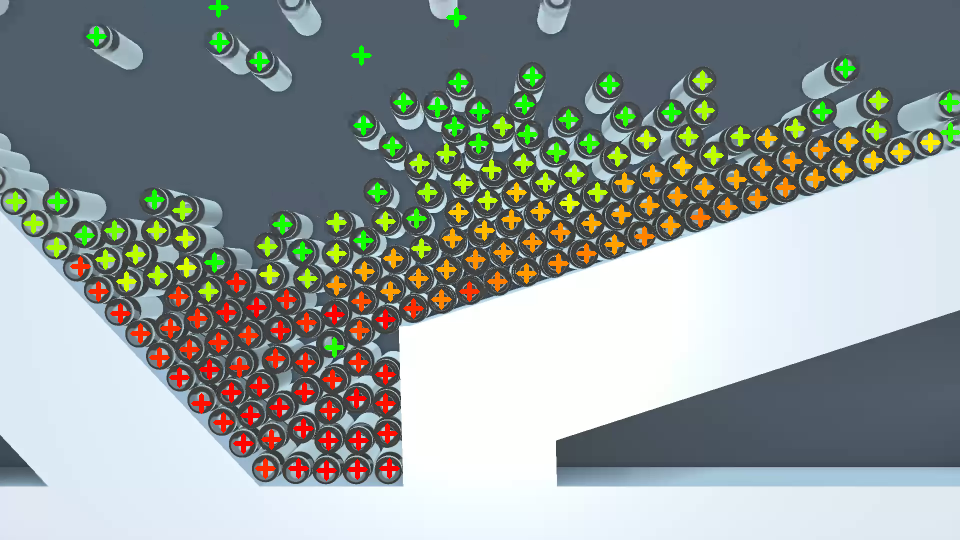
\includegraphics[width=0.45\linewidth]{images/Analysis_Cumulative.png}}}%
    \qquad %Add a line break to split into 2 vertically stacked images
    \subfloat[\centering Collision damage contribution visualisation \label{fig:analysis_damage_collision}]{{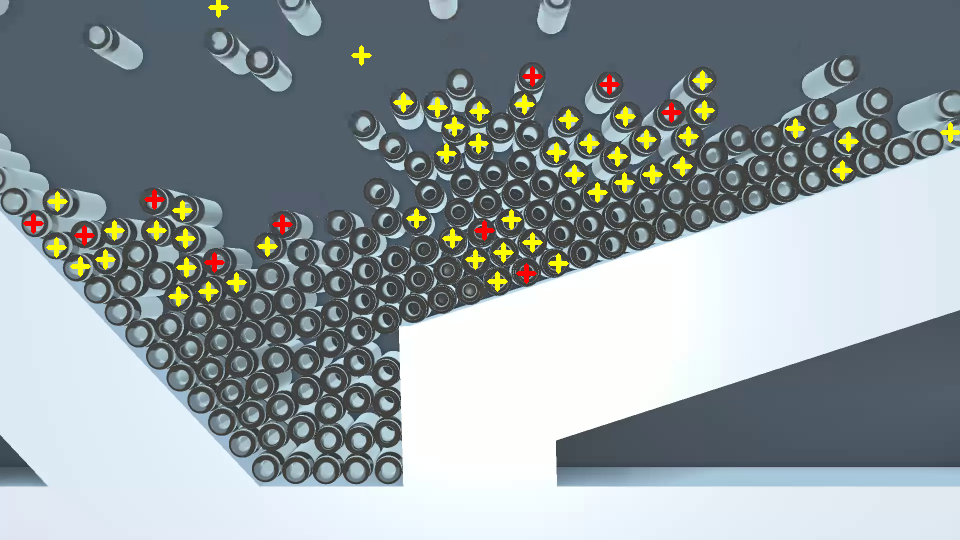
\includegraphics[width=0.45\linewidth]{images/Analysis_Collision.png}}}%
    \qquad %Add a line break to split into 2 vertically stacked images
    \caption{Damage assessment procedure (individual contributions)}
    \label{fig:analysis_damage_master}%
\end{figure}

The cumulative damage contribution is visualised in Figure \ref{fig:analysis_damage_cumulative} using a colour gradient from green to red to denote increasing residence time. Residence time extraction appears to be implemented effectively, presenting an accurate depiction of the historic behaviour of the system through residence time colourisation. The red accumulator basin suggests an initial migration towards this site, followed by an overspill of packs onto the right shoulder upon saturation (orange annotations), and a subsequent introduction of newer packs towards the top of the image (green annotations). These insights largely match the events of the simulation, supporting the functionality of this assessment stage, as well as indicating wider applicability of this technique. Aside from the contribution to the damage formulation, the residence time metric could be used to help visualise and understand product flow, with particular emphasis on identifying stagnation zones and regions of recirculation or turbulence, the presence of which may otherwise limit the throughput of the production line, or exaggerate accumulated damage.

The collision damage contribution is visualised in Figure \ref{fig:analysis_damage_collision} using red for primary collision targets (sources of abrupt acceleration change) and yellow for secondary targets (recipients of close-proximity damage propagation). Collision proposals are largely sensible, identifying sites that visually appear to be undergoing a collision event, such as initial impacts of introduced packs at the top of the image, and the collisions deeper within the accumulator likely resulting from a morphing pack arrangement. While this approach appears successful, it is noted that small inter-frame changes could provide a challenge due to the discrete nature of video feeds and subsequent rounding issues that affect these small scale impacts, which in themselves likely form the majority of collision events. 

The damage assessment pipeline demonstrates clear commercial value through the analytical capabilities offered at the constituent level, and the potential benefit of the combined formulation. The reliance on robust detection and tracking suggests rigorous tuning requirements for persistent damage and prevention of anomalous analysis results, such as those caused by false detections at the top of Figure \ref{fig:analysis_damage_cumulative} and \ref{fig:analysis_damage_collision}.

\subsubsection{Toppling Risk Assessment Procedure Evaluation}
The toppling risk assessment procedure analysed pack instability based on the size (area) and shape (regularity) of void regions. The output of a frame of analysis consisted of a colour-coded density map and textual summary, as shown in Figure \ref{fig:analysis_toppling_master}.

\begin{figure}[h]%
    \centering
    \subfloat[\centering Toppling risk assessment density map \label{fig:analysis_toppling_image}]{{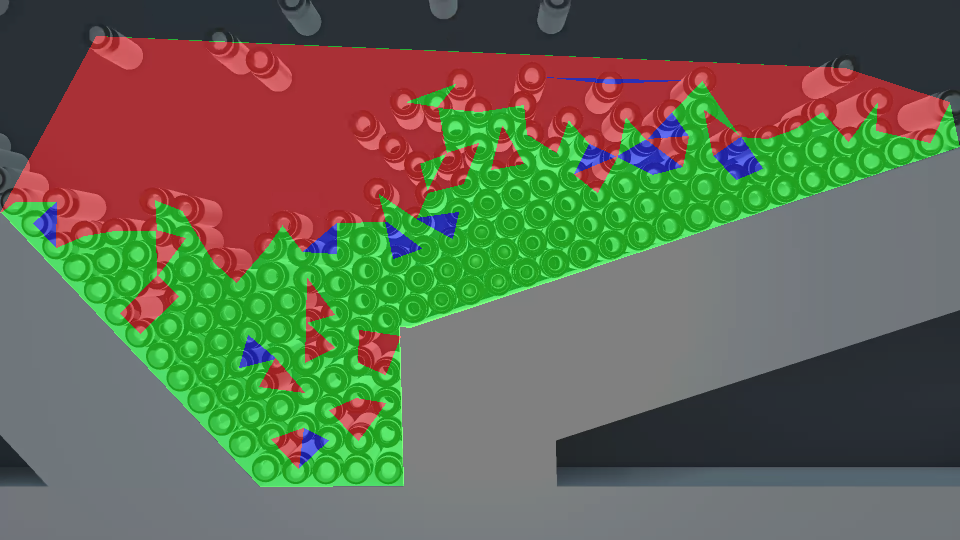
\includegraphics[width=0.45\linewidth, height=0.137\paperheight]{images/Analysis_Toppling.png}}}%
    \qquad %Add a line break to split into 2 vertically stacked images
    \subfloat[\centering Textual summary of toppling risk assessment \label{fig:analysis_toppling_summary}]{{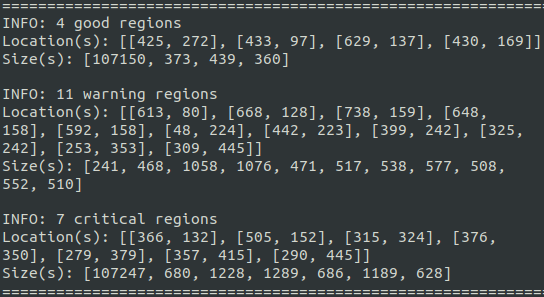
\includegraphics[width=0.45\linewidth, height=0.137\paperheight]{images/Analysis_Toppling_Summary.png}}}%
    \qquad %Add a line break to split into 2 vertically stacked images
    \caption{Toppling risk assessment procedure outputs}
    \label{fig:analysis_toppling_master}%
\end{figure}

Figure \ref{fig:analysis_toppling_image} demonstrates the method's ability to reliably identify voids and assess their relative stability. A clear difference in packing density is evident between the green (good) and red (critical) regions, corresponding to densely packed (stable) and more sparsely distributed (unstable) arrangements respectively. Several blue (warning) regions are also observed throughout the image, having little value at present due to the lack of calibration, however having the potential to identify early-stage void emergence if tuned accordingly. The critical and warning regions located within the stable zone are of particular interest, being more representative of a real-world scenario. These highlighted regions clearly show pack separation, demonstrating the procedure's effectiveness for automatically extracting these formations from within a crowded and complex frame. The subsequent summarised output (shown in Figure \ref{fig:analysis_toppling_summary}) successfully reduces the informational complexity and provides a more succinct indicator of line health, and one that is more readily interpretable by IT systems for improved compatibility and commercial feasibility. 


\subsection{Combined System Performance Evaluation}
A benchmark was performed to assess system performance, as presented in Figure \ref{fig:Overall_Performance_Profile}. The benchmark spanned 407 frames, with vials introduced at frame 55, followed by a periodic addition of batches of vials up to a maximum of 296 objects by the end of the benchmark. This is reflected in the performance plot, with a sharp increase at frame 55 followed by a periodic increase thereafter, resulting from an increased number of computations with additional objects.

\clearpage
\begin{figure}[ht]
    \begin{center}
        \resizebox{0.65\textwidth}{!}{
            %% Creator: Matplotlib, PGF backend
%%
%% To include the figure in your LaTeX document, write
%%   \input{<filename>.pgf}
%%
%% Make sure the required packages are loaded in your preamble
%%   \usepackage{pgf}
%%
%% and, on pdftex
%%   \usepackage[utf8]{inputenc}\DeclareUnicodeCharacter{2212}{-}
%%
%% or, on luatex and xetex
%%   \usepackage{unicode-math}
%%
%% Figures using additional raster images can only be included by \input if
%% they are in the same directory as the main LaTeX file. For loading figures
%% from other directories you can use the `import` package
%%   \usepackage{import}
%%
%% and then include the figures with
%%   \import{<path to file>}{<filename>.pgf}
%%
%% Matplotlib used the following preamble
%%
\begingroup%
\makeatletter%
\begin{pgfpicture}%
\pgfpathrectangle{\pgfpointorigin}{\pgfqpoint{6.000000in}{4.000000in}}%
\pgfusepath{use as bounding box, clip}%
\begin{pgfscope}%
\pgfsetbuttcap%
\pgfsetmiterjoin%
\pgfsetlinewidth{0.000000pt}%
\definecolor{currentstroke}{rgb}{1.000000,1.000000,1.000000}%
\pgfsetstrokecolor{currentstroke}%
\pgfsetstrokeopacity{0.000000}%
\pgfsetdash{}{0pt}%
\pgfpathmoveto{\pgfqpoint{0.000000in}{0.000000in}}%
\pgfpathlineto{\pgfqpoint{6.000000in}{0.000000in}}%
\pgfpathlineto{\pgfqpoint{6.000000in}{4.000000in}}%
\pgfpathlineto{\pgfqpoint{0.000000in}{4.000000in}}%
\pgfpathclose%
\pgfusepath{}%
\end{pgfscope}%
\begin{pgfscope}%
\pgfsetbuttcap%
\pgfsetmiterjoin%
\definecolor{currentfill}{rgb}{1.000000,1.000000,1.000000}%
\pgfsetfillcolor{currentfill}%
\pgfsetlinewidth{0.000000pt}%
\definecolor{currentstroke}{rgb}{0.000000,0.000000,0.000000}%
\pgfsetstrokecolor{currentstroke}%
\pgfsetstrokeopacity{0.000000}%
\pgfsetdash{}{0pt}%
\pgfpathmoveto{\pgfqpoint{0.759234in}{0.644073in}}%
\pgfpathlineto{\pgfqpoint{5.705740in}{0.644073in}}%
\pgfpathlineto{\pgfqpoint{5.705740in}{3.747130in}}%
\pgfpathlineto{\pgfqpoint{0.759234in}{3.747130in}}%
\pgfpathclose%
\pgfusepath{fill}%
\end{pgfscope}%
\begin{pgfscope}%
\pgfpathrectangle{\pgfqpoint{0.759234in}{0.644073in}}{\pgfqpoint{4.946506in}{3.103057in}}%
\pgfusepath{clip}%
\pgfsetbuttcap%
\pgfsetroundjoin%
\definecolor{currentfill}{rgb}{0.121569,0.466667,0.705882}%
\pgfsetfillcolor{currentfill}%
\pgfsetlinewidth{0.000000pt}%
\definecolor{currentstroke}{rgb}{0.000000,0.000000,0.000000}%
\pgfsetstrokecolor{currentstroke}%
\pgfsetdash{}{0pt}%
\pgfpathmoveto{\pgfqpoint{0.759234in}{0.829010in}}%
\pgfpathlineto{\pgfqpoint{0.759234in}{0.644073in}}%
\pgfpathlineto{\pgfqpoint{0.771538in}{0.644073in}}%
\pgfpathlineto{\pgfqpoint{0.783843in}{0.644073in}}%
\pgfpathlineto{\pgfqpoint{0.796148in}{0.644073in}}%
\pgfpathlineto{\pgfqpoint{0.808453in}{0.644073in}}%
\pgfpathlineto{\pgfqpoint{0.820757in}{0.644073in}}%
\pgfpathlineto{\pgfqpoint{0.833062in}{0.644073in}}%
\pgfpathlineto{\pgfqpoint{0.845367in}{0.644073in}}%
\pgfpathlineto{\pgfqpoint{0.857672in}{0.644073in}}%
\pgfpathlineto{\pgfqpoint{0.869976in}{0.644073in}}%
\pgfpathlineto{\pgfqpoint{0.882281in}{0.644073in}}%
\pgfpathlineto{\pgfqpoint{0.894586in}{0.644073in}}%
\pgfpathlineto{\pgfqpoint{0.906891in}{0.644073in}}%
\pgfpathlineto{\pgfqpoint{0.919195in}{0.644073in}}%
\pgfpathlineto{\pgfqpoint{0.931500in}{0.644073in}}%
\pgfpathlineto{\pgfqpoint{0.943805in}{0.644073in}}%
\pgfpathlineto{\pgfqpoint{0.956109in}{0.644073in}}%
\pgfpathlineto{\pgfqpoint{0.968414in}{0.644073in}}%
\pgfpathlineto{\pgfqpoint{0.980719in}{0.644073in}}%
\pgfpathlineto{\pgfqpoint{0.993024in}{0.644073in}}%
\pgfpathlineto{\pgfqpoint{1.005328in}{0.644073in}}%
\pgfpathlineto{\pgfqpoint{1.017633in}{0.644073in}}%
\pgfpathlineto{\pgfqpoint{1.029938in}{0.644073in}}%
\pgfpathlineto{\pgfqpoint{1.042243in}{0.644073in}}%
\pgfpathlineto{\pgfqpoint{1.054547in}{0.644073in}}%
\pgfpathlineto{\pgfqpoint{1.066852in}{0.644073in}}%
\pgfpathlineto{\pgfqpoint{1.079157in}{0.644073in}}%
\pgfpathlineto{\pgfqpoint{1.091462in}{0.644073in}}%
\pgfpathlineto{\pgfqpoint{1.103766in}{0.644073in}}%
\pgfpathlineto{\pgfqpoint{1.116071in}{0.644073in}}%
\pgfpathlineto{\pgfqpoint{1.128376in}{0.644073in}}%
\pgfpathlineto{\pgfqpoint{1.140681in}{0.644073in}}%
\pgfpathlineto{\pgfqpoint{1.152985in}{0.644073in}}%
\pgfpathlineto{\pgfqpoint{1.165290in}{0.644073in}}%
\pgfpathlineto{\pgfqpoint{1.177595in}{0.644073in}}%
\pgfpathlineto{\pgfqpoint{1.189900in}{0.644073in}}%
\pgfpathlineto{\pgfqpoint{1.202204in}{0.644073in}}%
\pgfpathlineto{\pgfqpoint{1.214509in}{0.644073in}}%
\pgfpathlineto{\pgfqpoint{1.226814in}{0.644073in}}%
\pgfpathlineto{\pgfqpoint{1.239119in}{0.644073in}}%
\pgfpathlineto{\pgfqpoint{1.251423in}{0.644073in}}%
\pgfpathlineto{\pgfqpoint{1.263728in}{0.644073in}}%
\pgfpathlineto{\pgfqpoint{1.276033in}{0.644073in}}%
\pgfpathlineto{\pgfqpoint{1.288338in}{0.644073in}}%
\pgfpathlineto{\pgfqpoint{1.300642in}{0.644073in}}%
\pgfpathlineto{\pgfqpoint{1.312947in}{0.644073in}}%
\pgfpathlineto{\pgfqpoint{1.325252in}{0.644073in}}%
\pgfpathlineto{\pgfqpoint{1.337556in}{0.644073in}}%
\pgfpathlineto{\pgfqpoint{1.349861in}{0.644073in}}%
\pgfpathlineto{\pgfqpoint{1.362166in}{0.644073in}}%
\pgfpathlineto{\pgfqpoint{1.374471in}{0.644073in}}%
\pgfpathlineto{\pgfqpoint{1.386775in}{0.644073in}}%
\pgfpathlineto{\pgfqpoint{1.399080in}{0.644073in}}%
\pgfpathlineto{\pgfqpoint{1.411385in}{0.644073in}}%
\pgfpathlineto{\pgfqpoint{1.423690in}{0.644073in}}%
\pgfpathlineto{\pgfqpoint{1.435994in}{0.644073in}}%
\pgfpathlineto{\pgfqpoint{1.448299in}{0.644073in}}%
\pgfpathlineto{\pgfqpoint{1.460604in}{0.644073in}}%
\pgfpathlineto{\pgfqpoint{1.472909in}{0.644073in}}%
\pgfpathlineto{\pgfqpoint{1.485213in}{0.644073in}}%
\pgfpathlineto{\pgfqpoint{1.497518in}{0.644073in}}%
\pgfpathlineto{\pgfqpoint{1.509823in}{0.644073in}}%
\pgfpathlineto{\pgfqpoint{1.522128in}{0.644073in}}%
\pgfpathlineto{\pgfqpoint{1.534432in}{0.644073in}}%
\pgfpathlineto{\pgfqpoint{1.546737in}{0.644073in}}%
\pgfpathlineto{\pgfqpoint{1.559042in}{0.644073in}}%
\pgfpathlineto{\pgfqpoint{1.571347in}{0.644073in}}%
\pgfpathlineto{\pgfqpoint{1.583651in}{0.644073in}}%
\pgfpathlineto{\pgfqpoint{1.595956in}{0.644073in}}%
\pgfpathlineto{\pgfqpoint{1.608261in}{0.644073in}}%
\pgfpathlineto{\pgfqpoint{1.620566in}{0.644073in}}%
\pgfpathlineto{\pgfqpoint{1.632870in}{0.644073in}}%
\pgfpathlineto{\pgfqpoint{1.645175in}{0.644073in}}%
\pgfpathlineto{\pgfqpoint{1.657480in}{0.644073in}}%
\pgfpathlineto{\pgfqpoint{1.669784in}{0.644073in}}%
\pgfpathlineto{\pgfqpoint{1.682089in}{0.644073in}}%
\pgfpathlineto{\pgfqpoint{1.694394in}{0.644073in}}%
\pgfpathlineto{\pgfqpoint{1.706699in}{0.644073in}}%
\pgfpathlineto{\pgfqpoint{1.719003in}{0.644073in}}%
\pgfpathlineto{\pgfqpoint{1.731308in}{0.644073in}}%
\pgfpathlineto{\pgfqpoint{1.743613in}{0.644073in}}%
\pgfpathlineto{\pgfqpoint{1.755918in}{0.644073in}}%
\pgfpathlineto{\pgfqpoint{1.768222in}{0.644073in}}%
\pgfpathlineto{\pgfqpoint{1.780527in}{0.644073in}}%
\pgfpathlineto{\pgfqpoint{1.792832in}{0.644073in}}%
\pgfpathlineto{\pgfqpoint{1.805137in}{0.644073in}}%
\pgfpathlineto{\pgfqpoint{1.817441in}{0.644073in}}%
\pgfpathlineto{\pgfqpoint{1.829746in}{0.644073in}}%
\pgfpathlineto{\pgfqpoint{1.842051in}{0.644073in}}%
\pgfpathlineto{\pgfqpoint{1.854356in}{0.644073in}}%
\pgfpathlineto{\pgfqpoint{1.866660in}{0.644073in}}%
\pgfpathlineto{\pgfqpoint{1.878965in}{0.644073in}}%
\pgfpathlineto{\pgfqpoint{1.891270in}{0.644073in}}%
\pgfpathlineto{\pgfqpoint{1.903575in}{0.644073in}}%
\pgfpathlineto{\pgfqpoint{1.915879in}{0.644073in}}%
\pgfpathlineto{\pgfqpoint{1.928184in}{0.644073in}}%
\pgfpathlineto{\pgfqpoint{1.940489in}{0.644073in}}%
\pgfpathlineto{\pgfqpoint{1.952794in}{0.644073in}}%
\pgfpathlineto{\pgfqpoint{1.965098in}{0.644073in}}%
\pgfpathlineto{\pgfqpoint{1.977403in}{0.644073in}}%
\pgfpathlineto{\pgfqpoint{1.989708in}{0.644073in}}%
\pgfpathlineto{\pgfqpoint{2.002013in}{0.644073in}}%
\pgfpathlineto{\pgfqpoint{2.014317in}{0.644073in}}%
\pgfpathlineto{\pgfqpoint{2.026622in}{0.644073in}}%
\pgfpathlineto{\pgfqpoint{2.038927in}{0.644073in}}%
\pgfpathlineto{\pgfqpoint{2.051231in}{0.644073in}}%
\pgfpathlineto{\pgfqpoint{2.063536in}{0.644073in}}%
\pgfpathlineto{\pgfqpoint{2.075841in}{0.644073in}}%
\pgfpathlineto{\pgfqpoint{2.088146in}{0.644073in}}%
\pgfpathlineto{\pgfqpoint{2.100450in}{0.644073in}}%
\pgfpathlineto{\pgfqpoint{2.112755in}{0.644073in}}%
\pgfpathlineto{\pgfqpoint{2.125060in}{0.644073in}}%
\pgfpathlineto{\pgfqpoint{2.137365in}{0.644073in}}%
\pgfpathlineto{\pgfqpoint{2.149669in}{0.644073in}}%
\pgfpathlineto{\pgfqpoint{2.161974in}{0.644073in}}%
\pgfpathlineto{\pgfqpoint{2.174279in}{0.644073in}}%
\pgfpathlineto{\pgfqpoint{2.186584in}{0.644073in}}%
\pgfpathlineto{\pgfqpoint{2.198888in}{0.644073in}}%
\pgfpathlineto{\pgfqpoint{2.211193in}{0.644073in}}%
\pgfpathlineto{\pgfqpoint{2.223498in}{0.644073in}}%
\pgfpathlineto{\pgfqpoint{2.235803in}{0.644073in}}%
\pgfpathlineto{\pgfqpoint{2.248107in}{0.644073in}}%
\pgfpathlineto{\pgfqpoint{2.260412in}{0.644073in}}%
\pgfpathlineto{\pgfqpoint{2.272717in}{0.644073in}}%
\pgfpathlineto{\pgfqpoint{2.285022in}{0.644073in}}%
\pgfpathlineto{\pgfqpoint{2.297326in}{0.644073in}}%
\pgfpathlineto{\pgfqpoint{2.309631in}{0.644073in}}%
\pgfpathlineto{\pgfqpoint{2.321936in}{0.644073in}}%
\pgfpathlineto{\pgfqpoint{2.334241in}{0.644073in}}%
\pgfpathlineto{\pgfqpoint{2.346545in}{0.644073in}}%
\pgfpathlineto{\pgfqpoint{2.358850in}{0.644073in}}%
\pgfpathlineto{\pgfqpoint{2.371155in}{0.644073in}}%
\pgfpathlineto{\pgfqpoint{2.383460in}{0.644073in}}%
\pgfpathlineto{\pgfqpoint{2.395764in}{0.644073in}}%
\pgfpathlineto{\pgfqpoint{2.408069in}{0.644073in}}%
\pgfpathlineto{\pgfqpoint{2.420374in}{0.644073in}}%
\pgfpathlineto{\pgfqpoint{2.432678in}{0.644073in}}%
\pgfpathlineto{\pgfqpoint{2.444983in}{0.644073in}}%
\pgfpathlineto{\pgfqpoint{2.457288in}{0.644073in}}%
\pgfpathlineto{\pgfqpoint{2.469593in}{0.644073in}}%
\pgfpathlineto{\pgfqpoint{2.481897in}{0.644073in}}%
\pgfpathlineto{\pgfqpoint{2.494202in}{0.644073in}}%
\pgfpathlineto{\pgfqpoint{2.506507in}{0.644073in}}%
\pgfpathlineto{\pgfqpoint{2.518812in}{0.644073in}}%
\pgfpathlineto{\pgfqpoint{2.531116in}{0.644073in}}%
\pgfpathlineto{\pgfqpoint{2.543421in}{0.644073in}}%
\pgfpathlineto{\pgfqpoint{2.555726in}{0.644073in}}%
\pgfpathlineto{\pgfqpoint{2.568031in}{0.644073in}}%
\pgfpathlineto{\pgfqpoint{2.580335in}{0.644073in}}%
\pgfpathlineto{\pgfqpoint{2.592640in}{0.644073in}}%
\pgfpathlineto{\pgfqpoint{2.604945in}{0.644073in}}%
\pgfpathlineto{\pgfqpoint{2.617250in}{0.644073in}}%
\pgfpathlineto{\pgfqpoint{2.629554in}{0.644073in}}%
\pgfpathlineto{\pgfqpoint{2.641859in}{0.644073in}}%
\pgfpathlineto{\pgfqpoint{2.654164in}{0.644073in}}%
\pgfpathlineto{\pgfqpoint{2.666469in}{0.644073in}}%
\pgfpathlineto{\pgfqpoint{2.678773in}{0.644073in}}%
\pgfpathlineto{\pgfqpoint{2.691078in}{0.644073in}}%
\pgfpathlineto{\pgfqpoint{2.703383in}{0.644073in}}%
\pgfpathlineto{\pgfqpoint{2.715688in}{0.644073in}}%
\pgfpathlineto{\pgfqpoint{2.727992in}{0.644073in}}%
\pgfpathlineto{\pgfqpoint{2.740297in}{0.644073in}}%
\pgfpathlineto{\pgfqpoint{2.752602in}{0.644073in}}%
\pgfpathlineto{\pgfqpoint{2.764906in}{0.644073in}}%
\pgfpathlineto{\pgfqpoint{2.777211in}{0.644073in}}%
\pgfpathlineto{\pgfqpoint{2.789516in}{0.644073in}}%
\pgfpathlineto{\pgfqpoint{2.801821in}{0.644073in}}%
\pgfpathlineto{\pgfqpoint{2.814125in}{0.644073in}}%
\pgfpathlineto{\pgfqpoint{2.826430in}{0.644073in}}%
\pgfpathlineto{\pgfqpoint{2.838735in}{0.644073in}}%
\pgfpathlineto{\pgfqpoint{2.851040in}{0.644073in}}%
\pgfpathlineto{\pgfqpoint{2.863344in}{0.644073in}}%
\pgfpathlineto{\pgfqpoint{2.875649in}{0.644073in}}%
\pgfpathlineto{\pgfqpoint{2.887954in}{0.644073in}}%
\pgfpathlineto{\pgfqpoint{2.900259in}{0.644073in}}%
\pgfpathlineto{\pgfqpoint{2.912563in}{0.644073in}}%
\pgfpathlineto{\pgfqpoint{2.924868in}{0.644073in}}%
\pgfpathlineto{\pgfqpoint{2.937173in}{0.644073in}}%
\pgfpathlineto{\pgfqpoint{2.949478in}{0.644073in}}%
\pgfpathlineto{\pgfqpoint{2.961782in}{0.644073in}}%
\pgfpathlineto{\pgfqpoint{2.974087in}{0.644073in}}%
\pgfpathlineto{\pgfqpoint{2.986392in}{0.644073in}}%
\pgfpathlineto{\pgfqpoint{2.998697in}{0.644073in}}%
\pgfpathlineto{\pgfqpoint{3.011001in}{0.644073in}}%
\pgfpathlineto{\pgfqpoint{3.023306in}{0.644073in}}%
\pgfpathlineto{\pgfqpoint{3.035611in}{0.644073in}}%
\pgfpathlineto{\pgfqpoint{3.047916in}{0.644073in}}%
\pgfpathlineto{\pgfqpoint{3.060220in}{0.644073in}}%
\pgfpathlineto{\pgfqpoint{3.072525in}{0.644073in}}%
\pgfpathlineto{\pgfqpoint{3.084830in}{0.644073in}}%
\pgfpathlineto{\pgfqpoint{3.097135in}{0.644073in}}%
\pgfpathlineto{\pgfqpoint{3.109439in}{0.644073in}}%
\pgfpathlineto{\pgfqpoint{3.121744in}{0.644073in}}%
\pgfpathlineto{\pgfqpoint{3.134049in}{0.644073in}}%
\pgfpathlineto{\pgfqpoint{3.146353in}{0.644073in}}%
\pgfpathlineto{\pgfqpoint{3.158658in}{0.644073in}}%
\pgfpathlineto{\pgfqpoint{3.170963in}{0.644073in}}%
\pgfpathlineto{\pgfqpoint{3.183268in}{0.644073in}}%
\pgfpathlineto{\pgfqpoint{3.195572in}{0.644073in}}%
\pgfpathlineto{\pgfqpoint{3.207877in}{0.644073in}}%
\pgfpathlineto{\pgfqpoint{3.220182in}{0.644073in}}%
\pgfpathlineto{\pgfqpoint{3.232487in}{0.644073in}}%
\pgfpathlineto{\pgfqpoint{3.244791in}{0.644073in}}%
\pgfpathlineto{\pgfqpoint{3.257096in}{0.644073in}}%
\pgfpathlineto{\pgfqpoint{3.269401in}{0.644073in}}%
\pgfpathlineto{\pgfqpoint{3.281706in}{0.644073in}}%
\pgfpathlineto{\pgfqpoint{3.294010in}{0.644073in}}%
\pgfpathlineto{\pgfqpoint{3.306315in}{0.644073in}}%
\pgfpathlineto{\pgfqpoint{3.318620in}{0.644073in}}%
\pgfpathlineto{\pgfqpoint{3.330925in}{0.644073in}}%
\pgfpathlineto{\pgfqpoint{3.343229in}{0.644073in}}%
\pgfpathlineto{\pgfqpoint{3.355534in}{0.644073in}}%
\pgfpathlineto{\pgfqpoint{3.367839in}{0.644073in}}%
\pgfpathlineto{\pgfqpoint{3.380144in}{0.644073in}}%
\pgfpathlineto{\pgfqpoint{3.392448in}{0.644073in}}%
\pgfpathlineto{\pgfqpoint{3.404753in}{0.644073in}}%
\pgfpathlineto{\pgfqpoint{3.417058in}{0.644073in}}%
\pgfpathlineto{\pgfqpoint{3.429363in}{0.644073in}}%
\pgfpathlineto{\pgfqpoint{3.441667in}{0.644073in}}%
\pgfpathlineto{\pgfqpoint{3.453972in}{0.644073in}}%
\pgfpathlineto{\pgfqpoint{3.466277in}{0.644073in}}%
\pgfpathlineto{\pgfqpoint{3.478582in}{0.644073in}}%
\pgfpathlineto{\pgfqpoint{3.490886in}{0.644073in}}%
\pgfpathlineto{\pgfqpoint{3.503191in}{0.644073in}}%
\pgfpathlineto{\pgfqpoint{3.515496in}{0.644073in}}%
\pgfpathlineto{\pgfqpoint{3.527800in}{0.644073in}}%
\pgfpathlineto{\pgfqpoint{3.540105in}{0.644073in}}%
\pgfpathlineto{\pgfqpoint{3.552410in}{0.644073in}}%
\pgfpathlineto{\pgfqpoint{3.564715in}{0.644073in}}%
\pgfpathlineto{\pgfqpoint{3.577019in}{0.644073in}}%
\pgfpathlineto{\pgfqpoint{3.589324in}{0.644073in}}%
\pgfpathlineto{\pgfqpoint{3.601629in}{0.644073in}}%
\pgfpathlineto{\pgfqpoint{3.613934in}{0.644073in}}%
\pgfpathlineto{\pgfqpoint{3.626238in}{0.644073in}}%
\pgfpathlineto{\pgfqpoint{3.638543in}{0.644073in}}%
\pgfpathlineto{\pgfqpoint{3.650848in}{0.644073in}}%
\pgfpathlineto{\pgfqpoint{3.663153in}{0.644073in}}%
\pgfpathlineto{\pgfqpoint{3.675457in}{0.644073in}}%
\pgfpathlineto{\pgfqpoint{3.687762in}{0.644073in}}%
\pgfpathlineto{\pgfqpoint{3.700067in}{0.644073in}}%
\pgfpathlineto{\pgfqpoint{3.712372in}{0.644073in}}%
\pgfpathlineto{\pgfqpoint{3.724676in}{0.644073in}}%
\pgfpathlineto{\pgfqpoint{3.736981in}{0.644073in}}%
\pgfpathlineto{\pgfqpoint{3.749286in}{0.644073in}}%
\pgfpathlineto{\pgfqpoint{3.761591in}{0.644073in}}%
\pgfpathlineto{\pgfqpoint{3.773895in}{0.644073in}}%
\pgfpathlineto{\pgfqpoint{3.786200in}{0.644073in}}%
\pgfpathlineto{\pgfqpoint{3.798505in}{0.644073in}}%
\pgfpathlineto{\pgfqpoint{3.810810in}{0.644073in}}%
\pgfpathlineto{\pgfqpoint{3.823114in}{0.644073in}}%
\pgfpathlineto{\pgfqpoint{3.835419in}{0.644073in}}%
\pgfpathlineto{\pgfqpoint{3.847724in}{0.644073in}}%
\pgfpathlineto{\pgfqpoint{3.860029in}{0.644073in}}%
\pgfpathlineto{\pgfqpoint{3.872333in}{0.644073in}}%
\pgfpathlineto{\pgfqpoint{3.884638in}{0.644073in}}%
\pgfpathlineto{\pgfqpoint{3.896943in}{0.644073in}}%
\pgfpathlineto{\pgfqpoint{3.909247in}{0.644073in}}%
\pgfpathlineto{\pgfqpoint{3.921552in}{0.644073in}}%
\pgfpathlineto{\pgfqpoint{3.933857in}{0.644073in}}%
\pgfpathlineto{\pgfqpoint{3.946162in}{0.644073in}}%
\pgfpathlineto{\pgfqpoint{3.958466in}{0.644073in}}%
\pgfpathlineto{\pgfqpoint{3.970771in}{0.644073in}}%
\pgfpathlineto{\pgfqpoint{3.983076in}{0.644073in}}%
\pgfpathlineto{\pgfqpoint{3.995381in}{0.644073in}}%
\pgfpathlineto{\pgfqpoint{4.007685in}{0.644073in}}%
\pgfpathlineto{\pgfqpoint{4.019990in}{0.644073in}}%
\pgfpathlineto{\pgfqpoint{4.032295in}{0.644073in}}%
\pgfpathlineto{\pgfqpoint{4.044600in}{0.644073in}}%
\pgfpathlineto{\pgfqpoint{4.056904in}{0.644073in}}%
\pgfpathlineto{\pgfqpoint{4.069209in}{0.644073in}}%
\pgfpathlineto{\pgfqpoint{4.081514in}{0.644073in}}%
\pgfpathlineto{\pgfqpoint{4.093819in}{0.644073in}}%
\pgfpathlineto{\pgfqpoint{4.106123in}{0.644073in}}%
\pgfpathlineto{\pgfqpoint{4.118428in}{0.644073in}}%
\pgfpathlineto{\pgfqpoint{4.130733in}{0.644073in}}%
\pgfpathlineto{\pgfqpoint{4.143038in}{0.644073in}}%
\pgfpathlineto{\pgfqpoint{4.155342in}{0.644073in}}%
\pgfpathlineto{\pgfqpoint{4.167647in}{0.644073in}}%
\pgfpathlineto{\pgfqpoint{4.179952in}{0.644073in}}%
\pgfpathlineto{\pgfqpoint{4.192257in}{0.644073in}}%
\pgfpathlineto{\pgfqpoint{4.204561in}{0.644073in}}%
\pgfpathlineto{\pgfqpoint{4.216866in}{0.644073in}}%
\pgfpathlineto{\pgfqpoint{4.229171in}{0.644073in}}%
\pgfpathlineto{\pgfqpoint{4.241475in}{0.644073in}}%
\pgfpathlineto{\pgfqpoint{4.253780in}{0.644073in}}%
\pgfpathlineto{\pgfqpoint{4.266085in}{0.644073in}}%
\pgfpathlineto{\pgfqpoint{4.278390in}{0.644073in}}%
\pgfpathlineto{\pgfqpoint{4.290694in}{0.644073in}}%
\pgfpathlineto{\pgfqpoint{4.302999in}{0.644073in}}%
\pgfpathlineto{\pgfqpoint{4.315304in}{0.644073in}}%
\pgfpathlineto{\pgfqpoint{4.327609in}{0.644073in}}%
\pgfpathlineto{\pgfqpoint{4.339913in}{0.644073in}}%
\pgfpathlineto{\pgfqpoint{4.352218in}{0.644073in}}%
\pgfpathlineto{\pgfqpoint{4.364523in}{0.644073in}}%
\pgfpathlineto{\pgfqpoint{4.376828in}{0.644073in}}%
\pgfpathlineto{\pgfqpoint{4.389132in}{0.644073in}}%
\pgfpathlineto{\pgfqpoint{4.401437in}{0.644073in}}%
\pgfpathlineto{\pgfqpoint{4.413742in}{0.644073in}}%
\pgfpathlineto{\pgfqpoint{4.426047in}{0.644073in}}%
\pgfpathlineto{\pgfqpoint{4.438351in}{0.644073in}}%
\pgfpathlineto{\pgfqpoint{4.450656in}{0.644073in}}%
\pgfpathlineto{\pgfqpoint{4.462961in}{0.644073in}}%
\pgfpathlineto{\pgfqpoint{4.475266in}{0.644073in}}%
\pgfpathlineto{\pgfqpoint{4.487570in}{0.644073in}}%
\pgfpathlineto{\pgfqpoint{4.499875in}{0.644073in}}%
\pgfpathlineto{\pgfqpoint{4.512180in}{0.644073in}}%
\pgfpathlineto{\pgfqpoint{4.524485in}{0.644073in}}%
\pgfpathlineto{\pgfqpoint{4.536789in}{0.644073in}}%
\pgfpathlineto{\pgfqpoint{4.549094in}{0.644073in}}%
\pgfpathlineto{\pgfqpoint{4.561399in}{0.644073in}}%
\pgfpathlineto{\pgfqpoint{4.573704in}{0.644073in}}%
\pgfpathlineto{\pgfqpoint{4.586008in}{0.644073in}}%
\pgfpathlineto{\pgfqpoint{4.598313in}{0.644073in}}%
\pgfpathlineto{\pgfqpoint{4.610618in}{0.644073in}}%
\pgfpathlineto{\pgfqpoint{4.622922in}{0.644073in}}%
\pgfpathlineto{\pgfqpoint{4.635227in}{0.644073in}}%
\pgfpathlineto{\pgfqpoint{4.647532in}{0.644073in}}%
\pgfpathlineto{\pgfqpoint{4.659837in}{0.644073in}}%
\pgfpathlineto{\pgfqpoint{4.672141in}{0.644073in}}%
\pgfpathlineto{\pgfqpoint{4.684446in}{0.644073in}}%
\pgfpathlineto{\pgfqpoint{4.696751in}{0.644073in}}%
\pgfpathlineto{\pgfqpoint{4.709056in}{0.644073in}}%
\pgfpathlineto{\pgfqpoint{4.721360in}{0.644073in}}%
\pgfpathlineto{\pgfqpoint{4.733665in}{0.644073in}}%
\pgfpathlineto{\pgfqpoint{4.745970in}{0.644073in}}%
\pgfpathlineto{\pgfqpoint{4.758275in}{0.644073in}}%
\pgfpathlineto{\pgfqpoint{4.770579in}{0.644073in}}%
\pgfpathlineto{\pgfqpoint{4.782884in}{0.644073in}}%
\pgfpathlineto{\pgfqpoint{4.795189in}{0.644073in}}%
\pgfpathlineto{\pgfqpoint{4.807494in}{0.644073in}}%
\pgfpathlineto{\pgfqpoint{4.819798in}{0.644073in}}%
\pgfpathlineto{\pgfqpoint{4.832103in}{0.644073in}}%
\pgfpathlineto{\pgfqpoint{4.844408in}{0.644073in}}%
\pgfpathlineto{\pgfqpoint{4.856713in}{0.644073in}}%
\pgfpathlineto{\pgfqpoint{4.869017in}{0.644073in}}%
\pgfpathlineto{\pgfqpoint{4.881322in}{0.644073in}}%
\pgfpathlineto{\pgfqpoint{4.893627in}{0.644073in}}%
\pgfpathlineto{\pgfqpoint{4.905932in}{0.644073in}}%
\pgfpathlineto{\pgfqpoint{4.918236in}{0.644073in}}%
\pgfpathlineto{\pgfqpoint{4.930541in}{0.644073in}}%
\pgfpathlineto{\pgfqpoint{4.942846in}{0.644073in}}%
\pgfpathlineto{\pgfqpoint{4.955151in}{0.644073in}}%
\pgfpathlineto{\pgfqpoint{4.967455in}{0.644073in}}%
\pgfpathlineto{\pgfqpoint{4.979760in}{0.644073in}}%
\pgfpathlineto{\pgfqpoint{4.992065in}{0.644073in}}%
\pgfpathlineto{\pgfqpoint{5.004369in}{0.644073in}}%
\pgfpathlineto{\pgfqpoint{5.016674in}{0.644073in}}%
\pgfpathlineto{\pgfqpoint{5.028979in}{0.644073in}}%
\pgfpathlineto{\pgfqpoint{5.041284in}{0.644073in}}%
\pgfpathlineto{\pgfqpoint{5.053588in}{0.644073in}}%
\pgfpathlineto{\pgfqpoint{5.065893in}{0.644073in}}%
\pgfpathlineto{\pgfqpoint{5.078198in}{0.644073in}}%
\pgfpathlineto{\pgfqpoint{5.090503in}{0.644073in}}%
\pgfpathlineto{\pgfqpoint{5.102807in}{0.644073in}}%
\pgfpathlineto{\pgfqpoint{5.115112in}{0.644073in}}%
\pgfpathlineto{\pgfqpoint{5.127417in}{0.644073in}}%
\pgfpathlineto{\pgfqpoint{5.139722in}{0.644073in}}%
\pgfpathlineto{\pgfqpoint{5.152026in}{0.644073in}}%
\pgfpathlineto{\pgfqpoint{5.164331in}{0.644073in}}%
\pgfpathlineto{\pgfqpoint{5.176636in}{0.644073in}}%
\pgfpathlineto{\pgfqpoint{5.188941in}{0.644073in}}%
\pgfpathlineto{\pgfqpoint{5.201245in}{0.644073in}}%
\pgfpathlineto{\pgfqpoint{5.213550in}{0.644073in}}%
\pgfpathlineto{\pgfqpoint{5.225855in}{0.644073in}}%
\pgfpathlineto{\pgfqpoint{5.238160in}{0.644073in}}%
\pgfpathlineto{\pgfqpoint{5.250464in}{0.644073in}}%
\pgfpathlineto{\pgfqpoint{5.262769in}{0.644073in}}%
\pgfpathlineto{\pgfqpoint{5.275074in}{0.644073in}}%
\pgfpathlineto{\pgfqpoint{5.287379in}{0.644073in}}%
\pgfpathlineto{\pgfqpoint{5.299683in}{0.644073in}}%
\pgfpathlineto{\pgfqpoint{5.311988in}{0.644073in}}%
\pgfpathlineto{\pgfqpoint{5.324293in}{0.644073in}}%
\pgfpathlineto{\pgfqpoint{5.336597in}{0.644073in}}%
\pgfpathlineto{\pgfqpoint{5.348902in}{0.644073in}}%
\pgfpathlineto{\pgfqpoint{5.361207in}{0.644073in}}%
\pgfpathlineto{\pgfqpoint{5.373512in}{0.644073in}}%
\pgfpathlineto{\pgfqpoint{5.385816in}{0.644073in}}%
\pgfpathlineto{\pgfqpoint{5.398121in}{0.644073in}}%
\pgfpathlineto{\pgfqpoint{5.410426in}{0.644073in}}%
\pgfpathlineto{\pgfqpoint{5.422731in}{0.644073in}}%
\pgfpathlineto{\pgfqpoint{5.435035in}{0.644073in}}%
\pgfpathlineto{\pgfqpoint{5.447340in}{0.644073in}}%
\pgfpathlineto{\pgfqpoint{5.459645in}{0.644073in}}%
\pgfpathlineto{\pgfqpoint{5.471950in}{0.644073in}}%
\pgfpathlineto{\pgfqpoint{5.484254in}{0.644073in}}%
\pgfpathlineto{\pgfqpoint{5.496559in}{0.644073in}}%
\pgfpathlineto{\pgfqpoint{5.508864in}{0.644073in}}%
\pgfpathlineto{\pgfqpoint{5.521169in}{0.644073in}}%
\pgfpathlineto{\pgfqpoint{5.533473in}{0.644073in}}%
\pgfpathlineto{\pgfqpoint{5.545778in}{0.644073in}}%
\pgfpathlineto{\pgfqpoint{5.558083in}{0.644073in}}%
\pgfpathlineto{\pgfqpoint{5.570388in}{0.644073in}}%
\pgfpathlineto{\pgfqpoint{5.582692in}{0.644073in}}%
\pgfpathlineto{\pgfqpoint{5.594997in}{0.644073in}}%
\pgfpathlineto{\pgfqpoint{5.607302in}{0.644073in}}%
\pgfpathlineto{\pgfqpoint{5.619607in}{0.644073in}}%
\pgfpathlineto{\pgfqpoint{5.631911in}{0.644073in}}%
\pgfpathlineto{\pgfqpoint{5.644216in}{0.644073in}}%
\pgfpathlineto{\pgfqpoint{5.656521in}{0.644073in}}%
\pgfpathlineto{\pgfqpoint{5.668826in}{0.644073in}}%
\pgfpathlineto{\pgfqpoint{5.681130in}{0.644073in}}%
\pgfpathlineto{\pgfqpoint{5.693435in}{0.644073in}}%
\pgfpathlineto{\pgfqpoint{5.705740in}{0.644073in}}%
\pgfpathlineto{\pgfqpoint{5.718044in}{0.644073in}}%
\pgfpathlineto{\pgfqpoint{5.718044in}{0.691662in}}%
\pgfpathlineto{\pgfqpoint{5.718044in}{0.691662in}}%
\pgfpathlineto{\pgfqpoint{5.705740in}{0.690785in}}%
\pgfpathlineto{\pgfqpoint{5.693435in}{0.690812in}}%
\pgfpathlineto{\pgfqpoint{5.681130in}{0.691565in}}%
\pgfpathlineto{\pgfqpoint{5.668826in}{0.689956in}}%
\pgfpathlineto{\pgfqpoint{5.656521in}{0.689493in}}%
\pgfpathlineto{\pgfqpoint{5.644216in}{0.693264in}}%
\pgfpathlineto{\pgfqpoint{5.631911in}{0.690403in}}%
\pgfpathlineto{\pgfqpoint{5.619607in}{0.690728in}}%
\pgfpathlineto{\pgfqpoint{5.607302in}{0.691020in}}%
\pgfpathlineto{\pgfqpoint{5.594997in}{0.692985in}}%
\pgfpathlineto{\pgfqpoint{5.582692in}{0.693445in}}%
\pgfpathlineto{\pgfqpoint{5.570388in}{0.695056in}}%
\pgfpathlineto{\pgfqpoint{5.558083in}{0.693942in}}%
\pgfpathlineto{\pgfqpoint{5.545778in}{0.695496in}}%
\pgfpathlineto{\pgfqpoint{5.533473in}{0.693310in}}%
\pgfpathlineto{\pgfqpoint{5.521169in}{0.695507in}}%
\pgfpathlineto{\pgfqpoint{5.508864in}{0.694856in}}%
\pgfpathlineto{\pgfqpoint{5.496559in}{0.696530in}}%
\pgfpathlineto{\pgfqpoint{5.484254in}{0.695565in}}%
\pgfpathlineto{\pgfqpoint{5.471950in}{0.695760in}}%
\pgfpathlineto{\pgfqpoint{5.459645in}{0.696253in}}%
\pgfpathlineto{\pgfqpoint{5.447340in}{0.695825in}}%
\pgfpathlineto{\pgfqpoint{5.435035in}{0.699204in}}%
\pgfpathlineto{\pgfqpoint{5.422731in}{0.695496in}}%
\pgfpathlineto{\pgfqpoint{5.410426in}{0.696441in}}%
\pgfpathlineto{\pgfqpoint{5.398121in}{0.691432in}}%
\pgfpathlineto{\pgfqpoint{5.385816in}{0.698701in}}%
\pgfpathlineto{\pgfqpoint{5.373512in}{0.692703in}}%
\pgfpathlineto{\pgfqpoint{5.361207in}{0.698883in}}%
\pgfpathlineto{\pgfqpoint{5.348902in}{0.694765in}}%
\pgfpathlineto{\pgfqpoint{5.336597in}{0.692745in}}%
\pgfpathlineto{\pgfqpoint{5.324293in}{0.698534in}}%
\pgfpathlineto{\pgfqpoint{5.311988in}{0.692112in}}%
\pgfpathlineto{\pgfqpoint{5.299683in}{0.695004in}}%
\pgfpathlineto{\pgfqpoint{5.287379in}{0.692868in}}%
\pgfpathlineto{\pgfqpoint{5.275074in}{0.696943in}}%
\pgfpathlineto{\pgfqpoint{5.262769in}{0.694818in}}%
\pgfpathlineto{\pgfqpoint{5.250464in}{0.695509in}}%
\pgfpathlineto{\pgfqpoint{5.238160in}{0.698727in}}%
\pgfpathlineto{\pgfqpoint{5.225855in}{0.692543in}}%
\pgfpathlineto{\pgfqpoint{5.213550in}{0.697050in}}%
\pgfpathlineto{\pgfqpoint{5.201245in}{0.692650in}}%
\pgfpathlineto{\pgfqpoint{5.188941in}{0.692694in}}%
\pgfpathlineto{\pgfqpoint{5.176636in}{0.692915in}}%
\pgfpathlineto{\pgfqpoint{5.164331in}{0.697186in}}%
\pgfpathlineto{\pgfqpoint{5.152026in}{0.693165in}}%
\pgfpathlineto{\pgfqpoint{5.139722in}{0.693363in}}%
\pgfpathlineto{\pgfqpoint{5.127417in}{0.696394in}}%
\pgfpathlineto{\pgfqpoint{5.115112in}{0.694064in}}%
\pgfpathlineto{\pgfqpoint{5.102807in}{0.692135in}}%
\pgfpathlineto{\pgfqpoint{5.090503in}{0.692300in}}%
\pgfpathlineto{\pgfqpoint{5.078198in}{0.696568in}}%
\pgfpathlineto{\pgfqpoint{5.065893in}{0.691363in}}%
\pgfpathlineto{\pgfqpoint{5.053588in}{0.695766in}}%
\pgfpathlineto{\pgfqpoint{5.041284in}{0.695149in}}%
\pgfpathlineto{\pgfqpoint{5.028979in}{0.696853in}}%
\pgfpathlineto{\pgfqpoint{5.016674in}{0.698057in}}%
\pgfpathlineto{\pgfqpoint{5.004369in}{0.694352in}}%
\pgfpathlineto{\pgfqpoint{4.992065in}{0.695856in}}%
\pgfpathlineto{\pgfqpoint{4.979760in}{0.699023in}}%
\pgfpathlineto{\pgfqpoint{4.967455in}{0.695483in}}%
\pgfpathlineto{\pgfqpoint{4.955151in}{0.696867in}}%
\pgfpathlineto{\pgfqpoint{4.942846in}{0.695747in}}%
\pgfpathlineto{\pgfqpoint{4.930541in}{0.700534in}}%
\pgfpathlineto{\pgfqpoint{4.918236in}{0.694712in}}%
\pgfpathlineto{\pgfqpoint{4.905932in}{0.694533in}}%
\pgfpathlineto{\pgfqpoint{4.893627in}{0.695182in}}%
\pgfpathlineto{\pgfqpoint{4.881322in}{0.701805in}}%
\pgfpathlineto{\pgfqpoint{4.869017in}{0.700331in}}%
\pgfpathlineto{\pgfqpoint{4.856713in}{0.697794in}}%
\pgfpathlineto{\pgfqpoint{4.844408in}{0.696885in}}%
\pgfpathlineto{\pgfqpoint{4.832103in}{0.701095in}}%
\pgfpathlineto{\pgfqpoint{4.819798in}{0.696711in}}%
\pgfpathlineto{\pgfqpoint{4.807494in}{0.702455in}}%
\pgfpathlineto{\pgfqpoint{4.795189in}{0.699391in}}%
\pgfpathlineto{\pgfqpoint{4.782884in}{0.695802in}}%
\pgfpathlineto{\pgfqpoint{4.770579in}{0.699010in}}%
\pgfpathlineto{\pgfqpoint{4.758275in}{0.697445in}}%
\pgfpathlineto{\pgfqpoint{4.745970in}{0.695235in}}%
\pgfpathlineto{\pgfqpoint{4.733665in}{0.693698in}}%
\pgfpathlineto{\pgfqpoint{4.721360in}{0.693314in}}%
\pgfpathlineto{\pgfqpoint{4.709056in}{0.693532in}}%
\pgfpathlineto{\pgfqpoint{4.696751in}{0.698188in}}%
\pgfpathlineto{\pgfqpoint{4.684446in}{0.702442in}}%
\pgfpathlineto{\pgfqpoint{4.672141in}{0.693290in}}%
\pgfpathlineto{\pgfqpoint{4.659837in}{0.696470in}}%
\pgfpathlineto{\pgfqpoint{4.647532in}{0.694228in}}%
\pgfpathlineto{\pgfqpoint{4.635227in}{0.697988in}}%
\pgfpathlineto{\pgfqpoint{4.622922in}{0.697372in}}%
\pgfpathlineto{\pgfqpoint{4.610618in}{0.695884in}}%
\pgfpathlineto{\pgfqpoint{4.598313in}{0.696052in}}%
\pgfpathlineto{\pgfqpoint{4.586008in}{0.696911in}}%
\pgfpathlineto{\pgfqpoint{4.573704in}{0.697455in}}%
\pgfpathlineto{\pgfqpoint{4.561399in}{0.702907in}}%
\pgfpathlineto{\pgfqpoint{4.549094in}{0.699819in}}%
\pgfpathlineto{\pgfqpoint{4.536789in}{0.693055in}}%
\pgfpathlineto{\pgfqpoint{4.524485in}{0.699063in}}%
\pgfpathlineto{\pgfqpoint{4.512180in}{0.695218in}}%
\pgfpathlineto{\pgfqpoint{4.499875in}{0.698678in}}%
\pgfpathlineto{\pgfqpoint{4.487570in}{0.702398in}}%
\pgfpathlineto{\pgfqpoint{4.475266in}{0.696437in}}%
\pgfpathlineto{\pgfqpoint{4.462961in}{0.697019in}}%
\pgfpathlineto{\pgfqpoint{4.450656in}{0.695151in}}%
\pgfpathlineto{\pgfqpoint{4.438351in}{0.694663in}}%
\pgfpathlineto{\pgfqpoint{4.426047in}{0.694846in}}%
\pgfpathlineto{\pgfqpoint{4.413742in}{0.694450in}}%
\pgfpathlineto{\pgfqpoint{4.401437in}{0.693448in}}%
\pgfpathlineto{\pgfqpoint{4.389132in}{0.691993in}}%
\pgfpathlineto{\pgfqpoint{4.376828in}{0.694100in}}%
\pgfpathlineto{\pgfqpoint{4.364523in}{0.692002in}}%
\pgfpathlineto{\pgfqpoint{4.352218in}{0.694853in}}%
\pgfpathlineto{\pgfqpoint{4.339913in}{0.693738in}}%
\pgfpathlineto{\pgfqpoint{4.327609in}{0.696039in}}%
\pgfpathlineto{\pgfqpoint{4.315304in}{0.694594in}}%
\pgfpathlineto{\pgfqpoint{4.302999in}{0.692987in}}%
\pgfpathlineto{\pgfqpoint{4.290694in}{0.697149in}}%
\pgfpathlineto{\pgfqpoint{4.278390in}{0.695826in}}%
\pgfpathlineto{\pgfqpoint{4.266085in}{0.701075in}}%
\pgfpathlineto{\pgfqpoint{4.253780in}{0.695843in}}%
\pgfpathlineto{\pgfqpoint{4.241475in}{0.695589in}}%
\pgfpathlineto{\pgfqpoint{4.229171in}{0.696222in}}%
\pgfpathlineto{\pgfqpoint{4.216866in}{0.696291in}}%
\pgfpathlineto{\pgfqpoint{4.204561in}{0.694096in}}%
\pgfpathlineto{\pgfqpoint{4.192257in}{0.692147in}}%
\pgfpathlineto{\pgfqpoint{4.179952in}{0.703307in}}%
\pgfpathlineto{\pgfqpoint{4.167647in}{0.695303in}}%
\pgfpathlineto{\pgfqpoint{4.155342in}{0.699288in}}%
\pgfpathlineto{\pgfqpoint{4.143038in}{0.693061in}}%
\pgfpathlineto{\pgfqpoint{4.130733in}{0.696085in}}%
\pgfpathlineto{\pgfqpoint{4.118428in}{0.695540in}}%
\pgfpathlineto{\pgfqpoint{4.106123in}{0.696737in}}%
\pgfpathlineto{\pgfqpoint{4.093819in}{0.701592in}}%
\pgfpathlineto{\pgfqpoint{4.081514in}{0.701317in}}%
\pgfpathlineto{\pgfqpoint{4.069209in}{0.697960in}}%
\pgfpathlineto{\pgfqpoint{4.056904in}{0.694149in}}%
\pgfpathlineto{\pgfqpoint{4.044600in}{0.693986in}}%
\pgfpathlineto{\pgfqpoint{4.032295in}{0.695412in}}%
\pgfpathlineto{\pgfqpoint{4.019990in}{0.692624in}}%
\pgfpathlineto{\pgfqpoint{4.007685in}{0.697273in}}%
\pgfpathlineto{\pgfqpoint{3.995381in}{0.693775in}}%
\pgfpathlineto{\pgfqpoint{3.983076in}{0.698121in}}%
\pgfpathlineto{\pgfqpoint{3.970771in}{0.693286in}}%
\pgfpathlineto{\pgfqpoint{3.958466in}{0.693581in}}%
\pgfpathlineto{\pgfqpoint{3.946162in}{0.692838in}}%
\pgfpathlineto{\pgfqpoint{3.933857in}{0.691576in}}%
\pgfpathlineto{\pgfqpoint{3.921552in}{0.700056in}}%
\pgfpathlineto{\pgfqpoint{3.909247in}{0.696987in}}%
\pgfpathlineto{\pgfqpoint{3.896943in}{0.694774in}}%
\pgfpathlineto{\pgfqpoint{3.884638in}{0.700268in}}%
\pgfpathlineto{\pgfqpoint{3.872333in}{0.696317in}}%
\pgfpathlineto{\pgfqpoint{3.860029in}{0.694079in}}%
\pgfpathlineto{\pgfqpoint{3.847724in}{0.693840in}}%
\pgfpathlineto{\pgfqpoint{3.835419in}{0.694608in}}%
\pgfpathlineto{\pgfqpoint{3.823114in}{0.695418in}}%
\pgfpathlineto{\pgfqpoint{3.810810in}{0.695530in}}%
\pgfpathlineto{\pgfqpoint{3.798505in}{0.695310in}}%
\pgfpathlineto{\pgfqpoint{3.786200in}{0.697729in}}%
\pgfpathlineto{\pgfqpoint{3.773895in}{0.700915in}}%
\pgfpathlineto{\pgfqpoint{3.761591in}{0.693703in}}%
\pgfpathlineto{\pgfqpoint{3.749286in}{0.700399in}}%
\pgfpathlineto{\pgfqpoint{3.736981in}{0.699552in}}%
\pgfpathlineto{\pgfqpoint{3.724676in}{0.696535in}}%
\pgfpathlineto{\pgfqpoint{3.712372in}{0.695722in}}%
\pgfpathlineto{\pgfqpoint{3.700067in}{0.698961in}}%
\pgfpathlineto{\pgfqpoint{3.687762in}{0.701270in}}%
\pgfpathlineto{\pgfqpoint{3.675457in}{0.691012in}}%
\pgfpathlineto{\pgfqpoint{3.663153in}{0.695241in}}%
\pgfpathlineto{\pgfqpoint{3.650848in}{0.694888in}}%
\pgfpathlineto{\pgfqpoint{3.638543in}{0.696947in}}%
\pgfpathlineto{\pgfqpoint{3.626238in}{0.693398in}}%
\pgfpathlineto{\pgfqpoint{3.613934in}{0.693547in}}%
\pgfpathlineto{\pgfqpoint{3.601629in}{0.696554in}}%
\pgfpathlineto{\pgfqpoint{3.589324in}{0.698420in}}%
\pgfpathlineto{\pgfqpoint{3.577019in}{0.694548in}}%
\pgfpathlineto{\pgfqpoint{3.564715in}{0.692897in}}%
\pgfpathlineto{\pgfqpoint{3.552410in}{0.694854in}}%
\pgfpathlineto{\pgfqpoint{3.540105in}{0.692976in}}%
\pgfpathlineto{\pgfqpoint{3.527800in}{0.694049in}}%
\pgfpathlineto{\pgfqpoint{3.515496in}{0.701690in}}%
\pgfpathlineto{\pgfqpoint{3.503191in}{0.697947in}}%
\pgfpathlineto{\pgfqpoint{3.490886in}{0.697959in}}%
\pgfpathlineto{\pgfqpoint{3.478582in}{0.695973in}}%
\pgfpathlineto{\pgfqpoint{3.466277in}{0.697410in}}%
\pgfpathlineto{\pgfqpoint{3.453972in}{0.696237in}}%
\pgfpathlineto{\pgfqpoint{3.441667in}{0.694502in}}%
\pgfpathlineto{\pgfqpoint{3.429363in}{0.692712in}}%
\pgfpathlineto{\pgfqpoint{3.417058in}{0.693920in}}%
\pgfpathlineto{\pgfqpoint{3.404753in}{0.698918in}}%
\pgfpathlineto{\pgfqpoint{3.392448in}{0.696030in}}%
\pgfpathlineto{\pgfqpoint{3.380144in}{0.699278in}}%
\pgfpathlineto{\pgfqpoint{3.367839in}{0.694917in}}%
\pgfpathlineto{\pgfqpoint{3.355534in}{0.700836in}}%
\pgfpathlineto{\pgfqpoint{3.343229in}{0.696012in}}%
\pgfpathlineto{\pgfqpoint{3.330925in}{0.702361in}}%
\pgfpathlineto{\pgfqpoint{3.318620in}{0.700255in}}%
\pgfpathlineto{\pgfqpoint{3.306315in}{0.697478in}}%
\pgfpathlineto{\pgfqpoint{3.294010in}{0.695764in}}%
\pgfpathlineto{\pgfqpoint{3.281706in}{0.702477in}}%
\pgfpathlineto{\pgfqpoint{3.269401in}{0.700282in}}%
\pgfpathlineto{\pgfqpoint{3.257096in}{0.700966in}}%
\pgfpathlineto{\pgfqpoint{3.244791in}{0.701761in}}%
\pgfpathlineto{\pgfqpoint{3.232487in}{0.695212in}}%
\pgfpathlineto{\pgfqpoint{3.220182in}{0.696735in}}%
\pgfpathlineto{\pgfqpoint{3.207877in}{0.699543in}}%
\pgfpathlineto{\pgfqpoint{3.195572in}{0.698409in}}%
\pgfpathlineto{\pgfqpoint{3.183268in}{0.697142in}}%
\pgfpathlineto{\pgfqpoint{3.170963in}{0.697581in}}%
\pgfpathlineto{\pgfqpoint{3.158658in}{0.697355in}}%
\pgfpathlineto{\pgfqpoint{3.146353in}{0.693869in}}%
\pgfpathlineto{\pgfqpoint{3.134049in}{0.695558in}}%
\pgfpathlineto{\pgfqpoint{3.121744in}{0.693512in}}%
\pgfpathlineto{\pgfqpoint{3.109439in}{0.697403in}}%
\pgfpathlineto{\pgfqpoint{3.097135in}{0.693812in}}%
\pgfpathlineto{\pgfqpoint{3.084830in}{0.698007in}}%
\pgfpathlineto{\pgfqpoint{3.072525in}{0.695526in}}%
\pgfpathlineto{\pgfqpoint{3.060220in}{0.697241in}}%
\pgfpathlineto{\pgfqpoint{3.047916in}{0.699736in}}%
\pgfpathlineto{\pgfqpoint{3.035611in}{0.697228in}}%
\pgfpathlineto{\pgfqpoint{3.023306in}{0.699946in}}%
\pgfpathlineto{\pgfqpoint{3.011001in}{0.699431in}}%
\pgfpathlineto{\pgfqpoint{2.998697in}{0.696431in}}%
\pgfpathlineto{\pgfqpoint{2.986392in}{0.693071in}}%
\pgfpathlineto{\pgfqpoint{2.974087in}{0.696503in}}%
\pgfpathlineto{\pgfqpoint{2.961782in}{0.695936in}}%
\pgfpathlineto{\pgfqpoint{2.949478in}{0.692082in}}%
\pgfpathlineto{\pgfqpoint{2.937173in}{0.694194in}}%
\pgfpathlineto{\pgfqpoint{2.924868in}{0.696359in}}%
\pgfpathlineto{\pgfqpoint{2.912563in}{0.701383in}}%
\pgfpathlineto{\pgfqpoint{2.900259in}{0.692781in}}%
\pgfpathlineto{\pgfqpoint{2.887954in}{0.695859in}}%
\pgfpathlineto{\pgfqpoint{2.875649in}{0.696360in}}%
\pgfpathlineto{\pgfqpoint{2.863344in}{0.696399in}}%
\pgfpathlineto{\pgfqpoint{2.851040in}{0.697656in}}%
\pgfpathlineto{\pgfqpoint{2.838735in}{0.696148in}}%
\pgfpathlineto{\pgfqpoint{2.826430in}{0.692609in}}%
\pgfpathlineto{\pgfqpoint{2.814125in}{0.696108in}}%
\pgfpathlineto{\pgfqpoint{2.801821in}{0.697478in}}%
\pgfpathlineto{\pgfqpoint{2.789516in}{0.694740in}}%
\pgfpathlineto{\pgfqpoint{2.777211in}{0.697603in}}%
\pgfpathlineto{\pgfqpoint{2.764906in}{0.701207in}}%
\pgfpathlineto{\pgfqpoint{2.752602in}{0.699383in}}%
\pgfpathlineto{\pgfqpoint{2.740297in}{0.694184in}}%
\pgfpathlineto{\pgfqpoint{2.727992in}{0.692208in}}%
\pgfpathlineto{\pgfqpoint{2.715688in}{0.697503in}}%
\pgfpathlineto{\pgfqpoint{2.703383in}{0.697101in}}%
\pgfpathlineto{\pgfqpoint{2.691078in}{0.697411in}}%
\pgfpathlineto{\pgfqpoint{2.678773in}{0.693735in}}%
\pgfpathlineto{\pgfqpoint{2.666469in}{0.693341in}}%
\pgfpathlineto{\pgfqpoint{2.654164in}{0.696134in}}%
\pgfpathlineto{\pgfqpoint{2.641859in}{0.695037in}}%
\pgfpathlineto{\pgfqpoint{2.629554in}{0.693329in}}%
\pgfpathlineto{\pgfqpoint{2.617250in}{0.697851in}}%
\pgfpathlineto{\pgfqpoint{2.604945in}{0.697208in}}%
\pgfpathlineto{\pgfqpoint{2.592640in}{0.698766in}}%
\pgfpathlineto{\pgfqpoint{2.580335in}{0.700929in}}%
\pgfpathlineto{\pgfqpoint{2.568031in}{0.694201in}}%
\pgfpathlineto{\pgfqpoint{2.555726in}{0.691940in}}%
\pgfpathlineto{\pgfqpoint{2.543421in}{0.692267in}}%
\pgfpathlineto{\pgfqpoint{2.531116in}{0.697540in}}%
\pgfpathlineto{\pgfqpoint{2.518812in}{0.701217in}}%
\pgfpathlineto{\pgfqpoint{2.506507in}{0.693447in}}%
\pgfpathlineto{\pgfqpoint{2.494202in}{0.701079in}}%
\pgfpathlineto{\pgfqpoint{2.481897in}{0.698846in}}%
\pgfpathlineto{\pgfqpoint{2.469593in}{0.695178in}}%
\pgfpathlineto{\pgfqpoint{2.457288in}{0.693181in}}%
\pgfpathlineto{\pgfqpoint{2.444983in}{0.695417in}}%
\pgfpathlineto{\pgfqpoint{2.432678in}{0.691754in}}%
\pgfpathlineto{\pgfqpoint{2.420374in}{0.698077in}}%
\pgfpathlineto{\pgfqpoint{2.408069in}{0.696082in}}%
\pgfpathlineto{\pgfqpoint{2.395764in}{0.693901in}}%
\pgfpathlineto{\pgfqpoint{2.383460in}{0.700303in}}%
\pgfpathlineto{\pgfqpoint{2.371155in}{0.693629in}}%
\pgfpathlineto{\pgfqpoint{2.358850in}{0.691865in}}%
\pgfpathlineto{\pgfqpoint{2.346545in}{0.693995in}}%
\pgfpathlineto{\pgfqpoint{2.334241in}{0.695318in}}%
\pgfpathlineto{\pgfqpoint{2.321936in}{0.699734in}}%
\pgfpathlineto{\pgfqpoint{2.309631in}{0.693231in}}%
\pgfpathlineto{\pgfqpoint{2.297326in}{0.692715in}}%
\pgfpathlineto{\pgfqpoint{2.285022in}{0.694635in}}%
\pgfpathlineto{\pgfqpoint{2.272717in}{0.692855in}}%
\pgfpathlineto{\pgfqpoint{2.260412in}{0.695726in}}%
\pgfpathlineto{\pgfqpoint{2.248107in}{0.695347in}}%
\pgfpathlineto{\pgfqpoint{2.235803in}{0.696192in}}%
\pgfpathlineto{\pgfqpoint{2.223498in}{0.692489in}}%
\pgfpathlineto{\pgfqpoint{2.211193in}{0.696037in}}%
\pgfpathlineto{\pgfqpoint{2.198888in}{0.693636in}}%
\pgfpathlineto{\pgfqpoint{2.186584in}{0.700338in}}%
\pgfpathlineto{\pgfqpoint{2.174279in}{0.693490in}}%
\pgfpathlineto{\pgfqpoint{2.161974in}{0.692827in}}%
\pgfpathlineto{\pgfqpoint{2.149669in}{0.693521in}}%
\pgfpathlineto{\pgfqpoint{2.137365in}{0.695223in}}%
\pgfpathlineto{\pgfqpoint{2.125060in}{0.691422in}}%
\pgfpathlineto{\pgfqpoint{2.112755in}{0.694435in}}%
\pgfpathlineto{\pgfqpoint{2.100450in}{0.697021in}}%
\pgfpathlineto{\pgfqpoint{2.088146in}{0.693678in}}%
\pgfpathlineto{\pgfqpoint{2.075841in}{0.696753in}}%
\pgfpathlineto{\pgfqpoint{2.063536in}{0.692455in}}%
\pgfpathlineto{\pgfqpoint{2.051231in}{0.693763in}}%
\pgfpathlineto{\pgfqpoint{2.038927in}{0.694106in}}%
\pgfpathlineto{\pgfqpoint{2.026622in}{0.693210in}}%
\pgfpathlineto{\pgfqpoint{2.014317in}{0.698487in}}%
\pgfpathlineto{\pgfqpoint{2.002013in}{0.691884in}}%
\pgfpathlineto{\pgfqpoint{1.989708in}{0.705594in}}%
\pgfpathlineto{\pgfqpoint{1.977403in}{0.693270in}}%
\pgfpathlineto{\pgfqpoint{1.965098in}{0.692605in}}%
\pgfpathlineto{\pgfqpoint{1.952794in}{0.692776in}}%
\pgfpathlineto{\pgfqpoint{1.940489in}{0.697553in}}%
\pgfpathlineto{\pgfqpoint{1.928184in}{0.698877in}}%
\pgfpathlineto{\pgfqpoint{1.915879in}{0.694372in}}%
\pgfpathlineto{\pgfqpoint{1.903575in}{0.694562in}}%
\pgfpathlineto{\pgfqpoint{1.891270in}{0.693742in}}%
\pgfpathlineto{\pgfqpoint{1.878965in}{0.696281in}}%
\pgfpathlineto{\pgfqpoint{1.866660in}{0.692302in}}%
\pgfpathlineto{\pgfqpoint{1.854356in}{0.693703in}}%
\pgfpathlineto{\pgfqpoint{1.842051in}{0.694020in}}%
\pgfpathlineto{\pgfqpoint{1.829746in}{0.693855in}}%
\pgfpathlineto{\pgfqpoint{1.817441in}{0.697069in}}%
\pgfpathlineto{\pgfqpoint{1.805137in}{0.694110in}}%
\pgfpathlineto{\pgfqpoint{1.792832in}{0.700104in}}%
\pgfpathlineto{\pgfqpoint{1.780527in}{0.692905in}}%
\pgfpathlineto{\pgfqpoint{1.768222in}{0.696110in}}%
\pgfpathlineto{\pgfqpoint{1.755918in}{0.697340in}}%
\pgfpathlineto{\pgfqpoint{1.743613in}{0.696825in}}%
\pgfpathlineto{\pgfqpoint{1.731308in}{0.699039in}}%
\pgfpathlineto{\pgfqpoint{1.719003in}{0.697682in}}%
\pgfpathlineto{\pgfqpoint{1.706699in}{0.701121in}}%
\pgfpathlineto{\pgfqpoint{1.694394in}{0.693374in}}%
\pgfpathlineto{\pgfqpoint{1.682089in}{0.697901in}}%
\pgfpathlineto{\pgfqpoint{1.669784in}{0.695561in}}%
\pgfpathlineto{\pgfqpoint{1.657480in}{0.700470in}}%
\pgfpathlineto{\pgfqpoint{1.645175in}{0.694547in}}%
\pgfpathlineto{\pgfqpoint{1.632870in}{0.693711in}}%
\pgfpathlineto{\pgfqpoint{1.620566in}{0.697834in}}%
\pgfpathlineto{\pgfqpoint{1.608261in}{0.695401in}}%
\pgfpathlineto{\pgfqpoint{1.595956in}{0.700190in}}%
\pgfpathlineto{\pgfqpoint{1.583651in}{0.696460in}}%
\pgfpathlineto{\pgfqpoint{1.571347in}{0.695468in}}%
\pgfpathlineto{\pgfqpoint{1.559042in}{0.699355in}}%
\pgfpathlineto{\pgfqpoint{1.546737in}{0.693293in}}%
\pgfpathlineto{\pgfqpoint{1.534432in}{0.695413in}}%
\pgfpathlineto{\pgfqpoint{1.522128in}{0.698070in}}%
\pgfpathlineto{\pgfqpoint{1.509823in}{0.695131in}}%
\pgfpathlineto{\pgfqpoint{1.497518in}{0.695593in}}%
\pgfpathlineto{\pgfqpoint{1.485213in}{0.697793in}}%
\pgfpathlineto{\pgfqpoint{1.472909in}{0.694764in}}%
\pgfpathlineto{\pgfqpoint{1.460604in}{0.695570in}}%
\pgfpathlineto{\pgfqpoint{1.448299in}{0.694507in}}%
\pgfpathlineto{\pgfqpoint{1.435994in}{0.696399in}}%
\pgfpathlineto{\pgfqpoint{1.423690in}{0.694561in}}%
\pgfpathlineto{\pgfqpoint{1.411385in}{0.696339in}}%
\pgfpathlineto{\pgfqpoint{1.399080in}{0.701203in}}%
\pgfpathlineto{\pgfqpoint{1.386775in}{0.696431in}}%
\pgfpathlineto{\pgfqpoint{1.374471in}{0.694998in}}%
\pgfpathlineto{\pgfqpoint{1.362166in}{0.696168in}}%
\pgfpathlineto{\pgfqpoint{1.349861in}{0.694029in}}%
\pgfpathlineto{\pgfqpoint{1.337556in}{0.696059in}}%
\pgfpathlineto{\pgfqpoint{1.325252in}{0.699101in}}%
\pgfpathlineto{\pgfqpoint{1.312947in}{0.702907in}}%
\pgfpathlineto{\pgfqpoint{1.300642in}{0.697771in}}%
\pgfpathlineto{\pgfqpoint{1.288338in}{0.702326in}}%
\pgfpathlineto{\pgfqpoint{1.276033in}{0.696774in}}%
\pgfpathlineto{\pgfqpoint{1.263728in}{0.696295in}}%
\pgfpathlineto{\pgfqpoint{1.251423in}{0.698872in}}%
\pgfpathlineto{\pgfqpoint{1.239119in}{0.698400in}}%
\pgfpathlineto{\pgfqpoint{1.226814in}{0.696106in}}%
\pgfpathlineto{\pgfqpoint{1.214509in}{0.703069in}}%
\pgfpathlineto{\pgfqpoint{1.202204in}{0.700926in}}%
\pgfpathlineto{\pgfqpoint{1.189900in}{0.698055in}}%
\pgfpathlineto{\pgfqpoint{1.177595in}{0.696697in}}%
\pgfpathlineto{\pgfqpoint{1.165290in}{0.698689in}}%
\pgfpathlineto{\pgfqpoint{1.152985in}{0.698184in}}%
\pgfpathlineto{\pgfqpoint{1.140681in}{0.700633in}}%
\pgfpathlineto{\pgfqpoint{1.128376in}{0.704341in}}%
\pgfpathlineto{\pgfqpoint{1.116071in}{0.699281in}}%
\pgfpathlineto{\pgfqpoint{1.103766in}{0.696815in}}%
\pgfpathlineto{\pgfqpoint{1.091462in}{0.699454in}}%
\pgfpathlineto{\pgfqpoint{1.079157in}{0.700291in}}%
\pgfpathlineto{\pgfqpoint{1.066852in}{0.705473in}}%
\pgfpathlineto{\pgfqpoint{1.054547in}{0.701395in}}%
\pgfpathlineto{\pgfqpoint{1.042243in}{0.702294in}}%
\pgfpathlineto{\pgfqpoint{1.029938in}{0.705241in}}%
\pgfpathlineto{\pgfqpoint{1.017633in}{0.697286in}}%
\pgfpathlineto{\pgfqpoint{1.005328in}{0.698808in}}%
\pgfpathlineto{\pgfqpoint{0.993024in}{0.697463in}}%
\pgfpathlineto{\pgfqpoint{0.980719in}{0.696476in}}%
\pgfpathlineto{\pgfqpoint{0.968414in}{0.702358in}}%
\pgfpathlineto{\pgfqpoint{0.956109in}{0.697951in}}%
\pgfpathlineto{\pgfqpoint{0.943805in}{0.698007in}}%
\pgfpathlineto{\pgfqpoint{0.931500in}{0.697003in}}%
\pgfpathlineto{\pgfqpoint{0.919195in}{0.702081in}}%
\pgfpathlineto{\pgfqpoint{0.906891in}{0.704215in}}%
\pgfpathlineto{\pgfqpoint{0.894586in}{0.705963in}}%
\pgfpathlineto{\pgfqpoint{0.882281in}{0.702935in}}%
\pgfpathlineto{\pgfqpoint{0.869976in}{0.703249in}}%
\pgfpathlineto{\pgfqpoint{0.857672in}{0.705520in}}%
\pgfpathlineto{\pgfqpoint{0.845367in}{0.697281in}}%
\pgfpathlineto{\pgfqpoint{0.833062in}{0.696757in}}%
\pgfpathlineto{\pgfqpoint{0.820757in}{0.709559in}}%
\pgfpathlineto{\pgfqpoint{0.808453in}{0.703224in}}%
\pgfpathlineto{\pgfqpoint{0.796148in}{0.703016in}}%
\pgfpathlineto{\pgfqpoint{0.783843in}{0.704428in}}%
\pgfpathlineto{\pgfqpoint{0.771538in}{0.700052in}}%
\pgfpathlineto{\pgfqpoint{0.759234in}{0.829010in}}%
\pgfpathclose%
\pgfusepath{fill}%
\end{pgfscope}%
\begin{pgfscope}%
\pgfpathrectangle{\pgfqpoint{0.759234in}{0.644073in}}{\pgfqpoint{4.946506in}{3.103057in}}%
\pgfusepath{clip}%
\pgfsetbuttcap%
\pgfsetroundjoin%
\definecolor{currentfill}{rgb}{1.000000,0.498039,0.054902}%
\pgfsetfillcolor{currentfill}%
\pgfsetlinewidth{0.000000pt}%
\definecolor{currentstroke}{rgb}{0.000000,0.000000,0.000000}%
\pgfsetstrokecolor{currentstroke}%
\pgfsetdash{}{0pt}%
\pgfpathmoveto{\pgfqpoint{0.759234in}{1.237514in}}%
\pgfpathlineto{\pgfqpoint{0.759234in}{0.829010in}}%
\pgfpathlineto{\pgfqpoint{0.771538in}{0.700052in}}%
\pgfpathlineto{\pgfqpoint{0.783843in}{0.704428in}}%
\pgfpathlineto{\pgfqpoint{0.796148in}{0.703016in}}%
\pgfpathlineto{\pgfqpoint{0.808453in}{0.703224in}}%
\pgfpathlineto{\pgfqpoint{0.820757in}{0.709559in}}%
\pgfpathlineto{\pgfqpoint{0.833062in}{0.696757in}}%
\pgfpathlineto{\pgfqpoint{0.845367in}{0.697281in}}%
\pgfpathlineto{\pgfqpoint{0.857672in}{0.705520in}}%
\pgfpathlineto{\pgfqpoint{0.869976in}{0.703249in}}%
\pgfpathlineto{\pgfqpoint{0.882281in}{0.702935in}}%
\pgfpathlineto{\pgfqpoint{0.894586in}{0.705963in}}%
\pgfpathlineto{\pgfqpoint{0.906891in}{0.704215in}}%
\pgfpathlineto{\pgfqpoint{0.919195in}{0.702081in}}%
\pgfpathlineto{\pgfqpoint{0.931500in}{0.697003in}}%
\pgfpathlineto{\pgfqpoint{0.943805in}{0.698007in}}%
\pgfpathlineto{\pgfqpoint{0.956109in}{0.697951in}}%
\pgfpathlineto{\pgfqpoint{0.968414in}{0.702358in}}%
\pgfpathlineto{\pgfqpoint{0.980719in}{0.696476in}}%
\pgfpathlineto{\pgfqpoint{0.993024in}{0.697463in}}%
\pgfpathlineto{\pgfqpoint{1.005328in}{0.698808in}}%
\pgfpathlineto{\pgfqpoint{1.017633in}{0.697286in}}%
\pgfpathlineto{\pgfqpoint{1.029938in}{0.705241in}}%
\pgfpathlineto{\pgfqpoint{1.042243in}{0.702294in}}%
\pgfpathlineto{\pgfqpoint{1.054547in}{0.701395in}}%
\pgfpathlineto{\pgfqpoint{1.066852in}{0.705473in}}%
\pgfpathlineto{\pgfqpoint{1.079157in}{0.700291in}}%
\pgfpathlineto{\pgfqpoint{1.091462in}{0.699454in}}%
\pgfpathlineto{\pgfqpoint{1.103766in}{0.696815in}}%
\pgfpathlineto{\pgfqpoint{1.116071in}{0.699281in}}%
\pgfpathlineto{\pgfqpoint{1.128376in}{0.704341in}}%
\pgfpathlineto{\pgfqpoint{1.140681in}{0.700633in}}%
\pgfpathlineto{\pgfqpoint{1.152985in}{0.698184in}}%
\pgfpathlineto{\pgfqpoint{1.165290in}{0.698689in}}%
\pgfpathlineto{\pgfqpoint{1.177595in}{0.696697in}}%
\pgfpathlineto{\pgfqpoint{1.189900in}{0.698055in}}%
\pgfpathlineto{\pgfqpoint{1.202204in}{0.700926in}}%
\pgfpathlineto{\pgfqpoint{1.214509in}{0.703069in}}%
\pgfpathlineto{\pgfqpoint{1.226814in}{0.696106in}}%
\pgfpathlineto{\pgfqpoint{1.239119in}{0.698400in}}%
\pgfpathlineto{\pgfqpoint{1.251423in}{0.698872in}}%
\pgfpathlineto{\pgfqpoint{1.263728in}{0.696295in}}%
\pgfpathlineto{\pgfqpoint{1.276033in}{0.696774in}}%
\pgfpathlineto{\pgfqpoint{1.288338in}{0.702326in}}%
\pgfpathlineto{\pgfqpoint{1.300642in}{0.697771in}}%
\pgfpathlineto{\pgfqpoint{1.312947in}{0.702907in}}%
\pgfpathlineto{\pgfqpoint{1.325252in}{0.699101in}}%
\pgfpathlineto{\pgfqpoint{1.337556in}{0.696059in}}%
\pgfpathlineto{\pgfqpoint{1.349861in}{0.694029in}}%
\pgfpathlineto{\pgfqpoint{1.362166in}{0.696168in}}%
\pgfpathlineto{\pgfqpoint{1.374471in}{0.694998in}}%
\pgfpathlineto{\pgfqpoint{1.386775in}{0.696431in}}%
\pgfpathlineto{\pgfqpoint{1.399080in}{0.701203in}}%
\pgfpathlineto{\pgfqpoint{1.411385in}{0.696339in}}%
\pgfpathlineto{\pgfqpoint{1.423690in}{0.694561in}}%
\pgfpathlineto{\pgfqpoint{1.435994in}{0.696399in}}%
\pgfpathlineto{\pgfqpoint{1.448299in}{0.694507in}}%
\pgfpathlineto{\pgfqpoint{1.460604in}{0.695570in}}%
\pgfpathlineto{\pgfqpoint{1.472909in}{0.694764in}}%
\pgfpathlineto{\pgfqpoint{1.485213in}{0.697793in}}%
\pgfpathlineto{\pgfqpoint{1.497518in}{0.695593in}}%
\pgfpathlineto{\pgfqpoint{1.509823in}{0.695131in}}%
\pgfpathlineto{\pgfqpoint{1.522128in}{0.698070in}}%
\pgfpathlineto{\pgfqpoint{1.534432in}{0.695413in}}%
\pgfpathlineto{\pgfqpoint{1.546737in}{0.693293in}}%
\pgfpathlineto{\pgfqpoint{1.559042in}{0.699355in}}%
\pgfpathlineto{\pgfqpoint{1.571347in}{0.695468in}}%
\pgfpathlineto{\pgfqpoint{1.583651in}{0.696460in}}%
\pgfpathlineto{\pgfqpoint{1.595956in}{0.700190in}}%
\pgfpathlineto{\pgfqpoint{1.608261in}{0.695401in}}%
\pgfpathlineto{\pgfqpoint{1.620566in}{0.697834in}}%
\pgfpathlineto{\pgfqpoint{1.632870in}{0.693711in}}%
\pgfpathlineto{\pgfqpoint{1.645175in}{0.694547in}}%
\pgfpathlineto{\pgfqpoint{1.657480in}{0.700470in}}%
\pgfpathlineto{\pgfqpoint{1.669784in}{0.695561in}}%
\pgfpathlineto{\pgfqpoint{1.682089in}{0.697901in}}%
\pgfpathlineto{\pgfqpoint{1.694394in}{0.693374in}}%
\pgfpathlineto{\pgfqpoint{1.706699in}{0.701121in}}%
\pgfpathlineto{\pgfqpoint{1.719003in}{0.697682in}}%
\pgfpathlineto{\pgfqpoint{1.731308in}{0.699039in}}%
\pgfpathlineto{\pgfqpoint{1.743613in}{0.696825in}}%
\pgfpathlineto{\pgfqpoint{1.755918in}{0.697340in}}%
\pgfpathlineto{\pgfqpoint{1.768222in}{0.696110in}}%
\pgfpathlineto{\pgfqpoint{1.780527in}{0.692905in}}%
\pgfpathlineto{\pgfqpoint{1.792832in}{0.700104in}}%
\pgfpathlineto{\pgfqpoint{1.805137in}{0.694110in}}%
\pgfpathlineto{\pgfqpoint{1.817441in}{0.697069in}}%
\pgfpathlineto{\pgfqpoint{1.829746in}{0.693855in}}%
\pgfpathlineto{\pgfqpoint{1.842051in}{0.694020in}}%
\pgfpathlineto{\pgfqpoint{1.854356in}{0.693703in}}%
\pgfpathlineto{\pgfqpoint{1.866660in}{0.692302in}}%
\pgfpathlineto{\pgfqpoint{1.878965in}{0.696281in}}%
\pgfpathlineto{\pgfqpoint{1.891270in}{0.693742in}}%
\pgfpathlineto{\pgfqpoint{1.903575in}{0.694562in}}%
\pgfpathlineto{\pgfqpoint{1.915879in}{0.694372in}}%
\pgfpathlineto{\pgfqpoint{1.928184in}{0.698877in}}%
\pgfpathlineto{\pgfqpoint{1.940489in}{0.697553in}}%
\pgfpathlineto{\pgfqpoint{1.952794in}{0.692776in}}%
\pgfpathlineto{\pgfqpoint{1.965098in}{0.692605in}}%
\pgfpathlineto{\pgfqpoint{1.977403in}{0.693270in}}%
\pgfpathlineto{\pgfqpoint{1.989708in}{0.705594in}}%
\pgfpathlineto{\pgfqpoint{2.002013in}{0.691884in}}%
\pgfpathlineto{\pgfqpoint{2.014317in}{0.698487in}}%
\pgfpathlineto{\pgfqpoint{2.026622in}{0.693210in}}%
\pgfpathlineto{\pgfqpoint{2.038927in}{0.694106in}}%
\pgfpathlineto{\pgfqpoint{2.051231in}{0.693763in}}%
\pgfpathlineto{\pgfqpoint{2.063536in}{0.692455in}}%
\pgfpathlineto{\pgfqpoint{2.075841in}{0.696753in}}%
\pgfpathlineto{\pgfqpoint{2.088146in}{0.693678in}}%
\pgfpathlineto{\pgfqpoint{2.100450in}{0.697021in}}%
\pgfpathlineto{\pgfqpoint{2.112755in}{0.694435in}}%
\pgfpathlineto{\pgfqpoint{2.125060in}{0.691422in}}%
\pgfpathlineto{\pgfqpoint{2.137365in}{0.695223in}}%
\pgfpathlineto{\pgfqpoint{2.149669in}{0.693521in}}%
\pgfpathlineto{\pgfqpoint{2.161974in}{0.692827in}}%
\pgfpathlineto{\pgfqpoint{2.174279in}{0.693490in}}%
\pgfpathlineto{\pgfqpoint{2.186584in}{0.700338in}}%
\pgfpathlineto{\pgfqpoint{2.198888in}{0.693636in}}%
\pgfpathlineto{\pgfqpoint{2.211193in}{0.696037in}}%
\pgfpathlineto{\pgfqpoint{2.223498in}{0.692489in}}%
\pgfpathlineto{\pgfqpoint{2.235803in}{0.696192in}}%
\pgfpathlineto{\pgfqpoint{2.248107in}{0.695347in}}%
\pgfpathlineto{\pgfqpoint{2.260412in}{0.695726in}}%
\pgfpathlineto{\pgfqpoint{2.272717in}{0.692855in}}%
\pgfpathlineto{\pgfqpoint{2.285022in}{0.694635in}}%
\pgfpathlineto{\pgfqpoint{2.297326in}{0.692715in}}%
\pgfpathlineto{\pgfqpoint{2.309631in}{0.693231in}}%
\pgfpathlineto{\pgfqpoint{2.321936in}{0.699734in}}%
\pgfpathlineto{\pgfqpoint{2.334241in}{0.695318in}}%
\pgfpathlineto{\pgfqpoint{2.346545in}{0.693995in}}%
\pgfpathlineto{\pgfqpoint{2.358850in}{0.691865in}}%
\pgfpathlineto{\pgfqpoint{2.371155in}{0.693629in}}%
\pgfpathlineto{\pgfqpoint{2.383460in}{0.700303in}}%
\pgfpathlineto{\pgfqpoint{2.395764in}{0.693901in}}%
\pgfpathlineto{\pgfqpoint{2.408069in}{0.696082in}}%
\pgfpathlineto{\pgfqpoint{2.420374in}{0.698077in}}%
\pgfpathlineto{\pgfqpoint{2.432678in}{0.691754in}}%
\pgfpathlineto{\pgfqpoint{2.444983in}{0.695417in}}%
\pgfpathlineto{\pgfqpoint{2.457288in}{0.693181in}}%
\pgfpathlineto{\pgfqpoint{2.469593in}{0.695178in}}%
\pgfpathlineto{\pgfqpoint{2.481897in}{0.698846in}}%
\pgfpathlineto{\pgfqpoint{2.494202in}{0.701079in}}%
\pgfpathlineto{\pgfqpoint{2.506507in}{0.693447in}}%
\pgfpathlineto{\pgfqpoint{2.518812in}{0.701217in}}%
\pgfpathlineto{\pgfqpoint{2.531116in}{0.697540in}}%
\pgfpathlineto{\pgfqpoint{2.543421in}{0.692267in}}%
\pgfpathlineto{\pgfqpoint{2.555726in}{0.691940in}}%
\pgfpathlineto{\pgfqpoint{2.568031in}{0.694201in}}%
\pgfpathlineto{\pgfqpoint{2.580335in}{0.700929in}}%
\pgfpathlineto{\pgfqpoint{2.592640in}{0.698766in}}%
\pgfpathlineto{\pgfqpoint{2.604945in}{0.697208in}}%
\pgfpathlineto{\pgfqpoint{2.617250in}{0.697851in}}%
\pgfpathlineto{\pgfqpoint{2.629554in}{0.693329in}}%
\pgfpathlineto{\pgfqpoint{2.641859in}{0.695037in}}%
\pgfpathlineto{\pgfqpoint{2.654164in}{0.696134in}}%
\pgfpathlineto{\pgfqpoint{2.666469in}{0.693341in}}%
\pgfpathlineto{\pgfqpoint{2.678773in}{0.693735in}}%
\pgfpathlineto{\pgfqpoint{2.691078in}{0.697411in}}%
\pgfpathlineto{\pgfqpoint{2.703383in}{0.697101in}}%
\pgfpathlineto{\pgfqpoint{2.715688in}{0.697503in}}%
\pgfpathlineto{\pgfqpoint{2.727992in}{0.692208in}}%
\pgfpathlineto{\pgfqpoint{2.740297in}{0.694184in}}%
\pgfpathlineto{\pgfqpoint{2.752602in}{0.699383in}}%
\pgfpathlineto{\pgfqpoint{2.764906in}{0.701207in}}%
\pgfpathlineto{\pgfqpoint{2.777211in}{0.697603in}}%
\pgfpathlineto{\pgfqpoint{2.789516in}{0.694740in}}%
\pgfpathlineto{\pgfqpoint{2.801821in}{0.697478in}}%
\pgfpathlineto{\pgfqpoint{2.814125in}{0.696108in}}%
\pgfpathlineto{\pgfqpoint{2.826430in}{0.692609in}}%
\pgfpathlineto{\pgfqpoint{2.838735in}{0.696148in}}%
\pgfpathlineto{\pgfqpoint{2.851040in}{0.697656in}}%
\pgfpathlineto{\pgfqpoint{2.863344in}{0.696399in}}%
\pgfpathlineto{\pgfqpoint{2.875649in}{0.696360in}}%
\pgfpathlineto{\pgfqpoint{2.887954in}{0.695859in}}%
\pgfpathlineto{\pgfqpoint{2.900259in}{0.692781in}}%
\pgfpathlineto{\pgfqpoint{2.912563in}{0.701383in}}%
\pgfpathlineto{\pgfqpoint{2.924868in}{0.696359in}}%
\pgfpathlineto{\pgfqpoint{2.937173in}{0.694194in}}%
\pgfpathlineto{\pgfqpoint{2.949478in}{0.692082in}}%
\pgfpathlineto{\pgfqpoint{2.961782in}{0.695936in}}%
\pgfpathlineto{\pgfqpoint{2.974087in}{0.696503in}}%
\pgfpathlineto{\pgfqpoint{2.986392in}{0.693071in}}%
\pgfpathlineto{\pgfqpoint{2.998697in}{0.696431in}}%
\pgfpathlineto{\pgfqpoint{3.011001in}{0.699431in}}%
\pgfpathlineto{\pgfqpoint{3.023306in}{0.699946in}}%
\pgfpathlineto{\pgfqpoint{3.035611in}{0.697228in}}%
\pgfpathlineto{\pgfqpoint{3.047916in}{0.699736in}}%
\pgfpathlineto{\pgfqpoint{3.060220in}{0.697241in}}%
\pgfpathlineto{\pgfqpoint{3.072525in}{0.695526in}}%
\pgfpathlineto{\pgfqpoint{3.084830in}{0.698007in}}%
\pgfpathlineto{\pgfqpoint{3.097135in}{0.693812in}}%
\pgfpathlineto{\pgfqpoint{3.109439in}{0.697403in}}%
\pgfpathlineto{\pgfqpoint{3.121744in}{0.693512in}}%
\pgfpathlineto{\pgfqpoint{3.134049in}{0.695558in}}%
\pgfpathlineto{\pgfqpoint{3.146353in}{0.693869in}}%
\pgfpathlineto{\pgfqpoint{3.158658in}{0.697355in}}%
\pgfpathlineto{\pgfqpoint{3.170963in}{0.697581in}}%
\pgfpathlineto{\pgfqpoint{3.183268in}{0.697142in}}%
\pgfpathlineto{\pgfqpoint{3.195572in}{0.698409in}}%
\pgfpathlineto{\pgfqpoint{3.207877in}{0.699543in}}%
\pgfpathlineto{\pgfqpoint{3.220182in}{0.696735in}}%
\pgfpathlineto{\pgfqpoint{3.232487in}{0.695212in}}%
\pgfpathlineto{\pgfqpoint{3.244791in}{0.701761in}}%
\pgfpathlineto{\pgfqpoint{3.257096in}{0.700966in}}%
\pgfpathlineto{\pgfqpoint{3.269401in}{0.700282in}}%
\pgfpathlineto{\pgfqpoint{3.281706in}{0.702477in}}%
\pgfpathlineto{\pgfqpoint{3.294010in}{0.695764in}}%
\pgfpathlineto{\pgfqpoint{3.306315in}{0.697478in}}%
\pgfpathlineto{\pgfqpoint{3.318620in}{0.700255in}}%
\pgfpathlineto{\pgfqpoint{3.330925in}{0.702361in}}%
\pgfpathlineto{\pgfqpoint{3.343229in}{0.696012in}}%
\pgfpathlineto{\pgfqpoint{3.355534in}{0.700836in}}%
\pgfpathlineto{\pgfqpoint{3.367839in}{0.694917in}}%
\pgfpathlineto{\pgfqpoint{3.380144in}{0.699278in}}%
\pgfpathlineto{\pgfqpoint{3.392448in}{0.696030in}}%
\pgfpathlineto{\pgfqpoint{3.404753in}{0.698918in}}%
\pgfpathlineto{\pgfqpoint{3.417058in}{0.693920in}}%
\pgfpathlineto{\pgfqpoint{3.429363in}{0.692712in}}%
\pgfpathlineto{\pgfqpoint{3.441667in}{0.694502in}}%
\pgfpathlineto{\pgfqpoint{3.453972in}{0.696237in}}%
\pgfpathlineto{\pgfqpoint{3.466277in}{0.697410in}}%
\pgfpathlineto{\pgfqpoint{3.478582in}{0.695973in}}%
\pgfpathlineto{\pgfqpoint{3.490886in}{0.697959in}}%
\pgfpathlineto{\pgfqpoint{3.503191in}{0.697947in}}%
\pgfpathlineto{\pgfqpoint{3.515496in}{0.701690in}}%
\pgfpathlineto{\pgfqpoint{3.527800in}{0.694049in}}%
\pgfpathlineto{\pgfqpoint{3.540105in}{0.692976in}}%
\pgfpathlineto{\pgfqpoint{3.552410in}{0.694854in}}%
\pgfpathlineto{\pgfqpoint{3.564715in}{0.692897in}}%
\pgfpathlineto{\pgfqpoint{3.577019in}{0.694548in}}%
\pgfpathlineto{\pgfqpoint{3.589324in}{0.698420in}}%
\pgfpathlineto{\pgfqpoint{3.601629in}{0.696554in}}%
\pgfpathlineto{\pgfqpoint{3.613934in}{0.693547in}}%
\pgfpathlineto{\pgfqpoint{3.626238in}{0.693398in}}%
\pgfpathlineto{\pgfqpoint{3.638543in}{0.696947in}}%
\pgfpathlineto{\pgfqpoint{3.650848in}{0.694888in}}%
\pgfpathlineto{\pgfqpoint{3.663153in}{0.695241in}}%
\pgfpathlineto{\pgfqpoint{3.675457in}{0.691012in}}%
\pgfpathlineto{\pgfqpoint{3.687762in}{0.701270in}}%
\pgfpathlineto{\pgfqpoint{3.700067in}{0.698961in}}%
\pgfpathlineto{\pgfqpoint{3.712372in}{0.695722in}}%
\pgfpathlineto{\pgfqpoint{3.724676in}{0.696535in}}%
\pgfpathlineto{\pgfqpoint{3.736981in}{0.699552in}}%
\pgfpathlineto{\pgfqpoint{3.749286in}{0.700399in}}%
\pgfpathlineto{\pgfqpoint{3.761591in}{0.693703in}}%
\pgfpathlineto{\pgfqpoint{3.773895in}{0.700915in}}%
\pgfpathlineto{\pgfqpoint{3.786200in}{0.697729in}}%
\pgfpathlineto{\pgfqpoint{3.798505in}{0.695310in}}%
\pgfpathlineto{\pgfqpoint{3.810810in}{0.695530in}}%
\pgfpathlineto{\pgfqpoint{3.823114in}{0.695418in}}%
\pgfpathlineto{\pgfqpoint{3.835419in}{0.694608in}}%
\pgfpathlineto{\pgfqpoint{3.847724in}{0.693840in}}%
\pgfpathlineto{\pgfqpoint{3.860029in}{0.694079in}}%
\pgfpathlineto{\pgfqpoint{3.872333in}{0.696317in}}%
\pgfpathlineto{\pgfqpoint{3.884638in}{0.700268in}}%
\pgfpathlineto{\pgfqpoint{3.896943in}{0.694774in}}%
\pgfpathlineto{\pgfqpoint{3.909247in}{0.696987in}}%
\pgfpathlineto{\pgfqpoint{3.921552in}{0.700056in}}%
\pgfpathlineto{\pgfqpoint{3.933857in}{0.691576in}}%
\pgfpathlineto{\pgfqpoint{3.946162in}{0.692838in}}%
\pgfpathlineto{\pgfqpoint{3.958466in}{0.693581in}}%
\pgfpathlineto{\pgfqpoint{3.970771in}{0.693286in}}%
\pgfpathlineto{\pgfqpoint{3.983076in}{0.698121in}}%
\pgfpathlineto{\pgfqpoint{3.995381in}{0.693775in}}%
\pgfpathlineto{\pgfqpoint{4.007685in}{0.697273in}}%
\pgfpathlineto{\pgfqpoint{4.019990in}{0.692624in}}%
\pgfpathlineto{\pgfqpoint{4.032295in}{0.695412in}}%
\pgfpathlineto{\pgfqpoint{4.044600in}{0.693986in}}%
\pgfpathlineto{\pgfqpoint{4.056904in}{0.694149in}}%
\pgfpathlineto{\pgfqpoint{4.069209in}{0.697960in}}%
\pgfpathlineto{\pgfqpoint{4.081514in}{0.701317in}}%
\pgfpathlineto{\pgfqpoint{4.093819in}{0.701592in}}%
\pgfpathlineto{\pgfqpoint{4.106123in}{0.696737in}}%
\pgfpathlineto{\pgfqpoint{4.118428in}{0.695540in}}%
\pgfpathlineto{\pgfqpoint{4.130733in}{0.696085in}}%
\pgfpathlineto{\pgfqpoint{4.143038in}{0.693061in}}%
\pgfpathlineto{\pgfqpoint{4.155342in}{0.699288in}}%
\pgfpathlineto{\pgfqpoint{4.167647in}{0.695303in}}%
\pgfpathlineto{\pgfqpoint{4.179952in}{0.703307in}}%
\pgfpathlineto{\pgfqpoint{4.192257in}{0.692147in}}%
\pgfpathlineto{\pgfqpoint{4.204561in}{0.694096in}}%
\pgfpathlineto{\pgfqpoint{4.216866in}{0.696291in}}%
\pgfpathlineto{\pgfqpoint{4.229171in}{0.696222in}}%
\pgfpathlineto{\pgfqpoint{4.241475in}{0.695589in}}%
\pgfpathlineto{\pgfqpoint{4.253780in}{0.695843in}}%
\pgfpathlineto{\pgfqpoint{4.266085in}{0.701075in}}%
\pgfpathlineto{\pgfqpoint{4.278390in}{0.695826in}}%
\pgfpathlineto{\pgfqpoint{4.290694in}{0.697149in}}%
\pgfpathlineto{\pgfqpoint{4.302999in}{0.692987in}}%
\pgfpathlineto{\pgfqpoint{4.315304in}{0.694594in}}%
\pgfpathlineto{\pgfqpoint{4.327609in}{0.696039in}}%
\pgfpathlineto{\pgfqpoint{4.339913in}{0.693738in}}%
\pgfpathlineto{\pgfqpoint{4.352218in}{0.694853in}}%
\pgfpathlineto{\pgfqpoint{4.364523in}{0.692002in}}%
\pgfpathlineto{\pgfqpoint{4.376828in}{0.694100in}}%
\pgfpathlineto{\pgfqpoint{4.389132in}{0.691993in}}%
\pgfpathlineto{\pgfqpoint{4.401437in}{0.693448in}}%
\pgfpathlineto{\pgfqpoint{4.413742in}{0.694450in}}%
\pgfpathlineto{\pgfqpoint{4.426047in}{0.694846in}}%
\pgfpathlineto{\pgfqpoint{4.438351in}{0.694663in}}%
\pgfpathlineto{\pgfqpoint{4.450656in}{0.695151in}}%
\pgfpathlineto{\pgfqpoint{4.462961in}{0.697019in}}%
\pgfpathlineto{\pgfqpoint{4.475266in}{0.696437in}}%
\pgfpathlineto{\pgfqpoint{4.487570in}{0.702398in}}%
\pgfpathlineto{\pgfqpoint{4.499875in}{0.698678in}}%
\pgfpathlineto{\pgfqpoint{4.512180in}{0.695218in}}%
\pgfpathlineto{\pgfqpoint{4.524485in}{0.699063in}}%
\pgfpathlineto{\pgfqpoint{4.536789in}{0.693055in}}%
\pgfpathlineto{\pgfqpoint{4.549094in}{0.699819in}}%
\pgfpathlineto{\pgfqpoint{4.561399in}{0.702907in}}%
\pgfpathlineto{\pgfqpoint{4.573704in}{0.697455in}}%
\pgfpathlineto{\pgfqpoint{4.586008in}{0.696911in}}%
\pgfpathlineto{\pgfqpoint{4.598313in}{0.696052in}}%
\pgfpathlineto{\pgfqpoint{4.610618in}{0.695884in}}%
\pgfpathlineto{\pgfqpoint{4.622922in}{0.697372in}}%
\pgfpathlineto{\pgfqpoint{4.635227in}{0.697988in}}%
\pgfpathlineto{\pgfqpoint{4.647532in}{0.694228in}}%
\pgfpathlineto{\pgfqpoint{4.659837in}{0.696470in}}%
\pgfpathlineto{\pgfqpoint{4.672141in}{0.693290in}}%
\pgfpathlineto{\pgfqpoint{4.684446in}{0.702442in}}%
\pgfpathlineto{\pgfqpoint{4.696751in}{0.698188in}}%
\pgfpathlineto{\pgfqpoint{4.709056in}{0.693532in}}%
\pgfpathlineto{\pgfqpoint{4.721360in}{0.693314in}}%
\pgfpathlineto{\pgfqpoint{4.733665in}{0.693698in}}%
\pgfpathlineto{\pgfqpoint{4.745970in}{0.695235in}}%
\pgfpathlineto{\pgfqpoint{4.758275in}{0.697445in}}%
\pgfpathlineto{\pgfqpoint{4.770579in}{0.699010in}}%
\pgfpathlineto{\pgfqpoint{4.782884in}{0.695802in}}%
\pgfpathlineto{\pgfqpoint{4.795189in}{0.699391in}}%
\pgfpathlineto{\pgfqpoint{4.807494in}{0.702455in}}%
\pgfpathlineto{\pgfqpoint{4.819798in}{0.696711in}}%
\pgfpathlineto{\pgfqpoint{4.832103in}{0.701095in}}%
\pgfpathlineto{\pgfqpoint{4.844408in}{0.696885in}}%
\pgfpathlineto{\pgfqpoint{4.856713in}{0.697794in}}%
\pgfpathlineto{\pgfqpoint{4.869017in}{0.700331in}}%
\pgfpathlineto{\pgfqpoint{4.881322in}{0.701805in}}%
\pgfpathlineto{\pgfqpoint{4.893627in}{0.695182in}}%
\pgfpathlineto{\pgfqpoint{4.905932in}{0.694533in}}%
\pgfpathlineto{\pgfqpoint{4.918236in}{0.694712in}}%
\pgfpathlineto{\pgfqpoint{4.930541in}{0.700534in}}%
\pgfpathlineto{\pgfqpoint{4.942846in}{0.695747in}}%
\pgfpathlineto{\pgfqpoint{4.955151in}{0.696867in}}%
\pgfpathlineto{\pgfqpoint{4.967455in}{0.695483in}}%
\pgfpathlineto{\pgfqpoint{4.979760in}{0.699023in}}%
\pgfpathlineto{\pgfqpoint{4.992065in}{0.695856in}}%
\pgfpathlineto{\pgfqpoint{5.004369in}{0.694352in}}%
\pgfpathlineto{\pgfqpoint{5.016674in}{0.698057in}}%
\pgfpathlineto{\pgfqpoint{5.028979in}{0.696853in}}%
\pgfpathlineto{\pgfqpoint{5.041284in}{0.695149in}}%
\pgfpathlineto{\pgfqpoint{5.053588in}{0.695766in}}%
\pgfpathlineto{\pgfqpoint{5.065893in}{0.691363in}}%
\pgfpathlineto{\pgfqpoint{5.078198in}{0.696568in}}%
\pgfpathlineto{\pgfqpoint{5.090503in}{0.692300in}}%
\pgfpathlineto{\pgfqpoint{5.102807in}{0.692135in}}%
\pgfpathlineto{\pgfqpoint{5.115112in}{0.694064in}}%
\pgfpathlineto{\pgfqpoint{5.127417in}{0.696394in}}%
\pgfpathlineto{\pgfqpoint{5.139722in}{0.693363in}}%
\pgfpathlineto{\pgfqpoint{5.152026in}{0.693165in}}%
\pgfpathlineto{\pgfqpoint{5.164331in}{0.697186in}}%
\pgfpathlineto{\pgfqpoint{5.176636in}{0.692915in}}%
\pgfpathlineto{\pgfqpoint{5.188941in}{0.692694in}}%
\pgfpathlineto{\pgfqpoint{5.201245in}{0.692650in}}%
\pgfpathlineto{\pgfqpoint{5.213550in}{0.697050in}}%
\pgfpathlineto{\pgfqpoint{5.225855in}{0.692543in}}%
\pgfpathlineto{\pgfqpoint{5.238160in}{0.698727in}}%
\pgfpathlineto{\pgfqpoint{5.250464in}{0.695509in}}%
\pgfpathlineto{\pgfqpoint{5.262769in}{0.694818in}}%
\pgfpathlineto{\pgfqpoint{5.275074in}{0.696943in}}%
\pgfpathlineto{\pgfqpoint{5.287379in}{0.692868in}}%
\pgfpathlineto{\pgfqpoint{5.299683in}{0.695004in}}%
\pgfpathlineto{\pgfqpoint{5.311988in}{0.692112in}}%
\pgfpathlineto{\pgfqpoint{5.324293in}{0.698534in}}%
\pgfpathlineto{\pgfqpoint{5.336597in}{0.692745in}}%
\pgfpathlineto{\pgfqpoint{5.348902in}{0.694765in}}%
\pgfpathlineto{\pgfqpoint{5.361207in}{0.698883in}}%
\pgfpathlineto{\pgfqpoint{5.373512in}{0.692703in}}%
\pgfpathlineto{\pgfqpoint{5.385816in}{0.698701in}}%
\pgfpathlineto{\pgfqpoint{5.398121in}{0.691432in}}%
\pgfpathlineto{\pgfqpoint{5.410426in}{0.696441in}}%
\pgfpathlineto{\pgfqpoint{5.422731in}{0.695496in}}%
\pgfpathlineto{\pgfqpoint{5.435035in}{0.699204in}}%
\pgfpathlineto{\pgfqpoint{5.447340in}{0.695825in}}%
\pgfpathlineto{\pgfqpoint{5.459645in}{0.696253in}}%
\pgfpathlineto{\pgfqpoint{5.471950in}{0.695760in}}%
\pgfpathlineto{\pgfqpoint{5.484254in}{0.695565in}}%
\pgfpathlineto{\pgfqpoint{5.496559in}{0.696530in}}%
\pgfpathlineto{\pgfqpoint{5.508864in}{0.694856in}}%
\pgfpathlineto{\pgfqpoint{5.521169in}{0.695507in}}%
\pgfpathlineto{\pgfqpoint{5.533473in}{0.693310in}}%
\pgfpathlineto{\pgfqpoint{5.545778in}{0.695496in}}%
\pgfpathlineto{\pgfqpoint{5.558083in}{0.693942in}}%
\pgfpathlineto{\pgfqpoint{5.570388in}{0.695056in}}%
\pgfpathlineto{\pgfqpoint{5.582692in}{0.693445in}}%
\pgfpathlineto{\pgfqpoint{5.594997in}{0.692985in}}%
\pgfpathlineto{\pgfqpoint{5.607302in}{0.691020in}}%
\pgfpathlineto{\pgfqpoint{5.619607in}{0.690728in}}%
\pgfpathlineto{\pgfqpoint{5.631911in}{0.690403in}}%
\pgfpathlineto{\pgfqpoint{5.644216in}{0.693264in}}%
\pgfpathlineto{\pgfqpoint{5.656521in}{0.689493in}}%
\pgfpathlineto{\pgfqpoint{5.668826in}{0.689956in}}%
\pgfpathlineto{\pgfqpoint{5.681130in}{0.691565in}}%
\pgfpathlineto{\pgfqpoint{5.693435in}{0.690812in}}%
\pgfpathlineto{\pgfqpoint{5.705740in}{0.690785in}}%
\pgfpathlineto{\pgfqpoint{5.718044in}{0.691662in}}%
\pgfpathlineto{\pgfqpoint{5.718044in}{1.338511in}}%
\pgfpathlineto{\pgfqpoint{5.718044in}{1.338511in}}%
\pgfpathlineto{\pgfqpoint{5.705740in}{1.346348in}}%
\pgfpathlineto{\pgfqpoint{5.693435in}{1.337414in}}%
\pgfpathlineto{\pgfqpoint{5.681130in}{1.338769in}}%
\pgfpathlineto{\pgfqpoint{5.668826in}{1.335412in}}%
\pgfpathlineto{\pgfqpoint{5.656521in}{1.344450in}}%
\pgfpathlineto{\pgfqpoint{5.644216in}{1.350418in}}%
\pgfpathlineto{\pgfqpoint{5.631911in}{1.338188in}}%
\pgfpathlineto{\pgfqpoint{5.619607in}{1.342974in}}%
\pgfpathlineto{\pgfqpoint{5.607302in}{1.338849in}}%
\pgfpathlineto{\pgfqpoint{5.594997in}{1.335447in}}%
\pgfpathlineto{\pgfqpoint{5.582692in}{1.343811in}}%
\pgfpathlineto{\pgfqpoint{5.570388in}{1.354722in}}%
\pgfpathlineto{\pgfqpoint{5.558083in}{1.356092in}}%
\pgfpathlineto{\pgfqpoint{5.545778in}{1.349910in}}%
\pgfpathlineto{\pgfqpoint{5.533473in}{1.340934in}}%
\pgfpathlineto{\pgfqpoint{5.521169in}{1.345548in}}%
\pgfpathlineto{\pgfqpoint{5.508864in}{1.349220in}}%
\pgfpathlineto{\pgfqpoint{5.496559in}{1.352228in}}%
\pgfpathlineto{\pgfqpoint{5.484254in}{1.358057in}}%
\pgfpathlineto{\pgfqpoint{5.471950in}{1.339236in}}%
\pgfpathlineto{\pgfqpoint{5.459645in}{1.357808in}}%
\pgfpathlineto{\pgfqpoint{5.447340in}{1.353912in}}%
\pgfpathlineto{\pgfqpoint{5.435035in}{1.350855in}}%
\pgfpathlineto{\pgfqpoint{5.422731in}{1.357806in}}%
\pgfpathlineto{\pgfqpoint{5.410426in}{1.348020in}}%
\pgfpathlineto{\pgfqpoint{5.398121in}{1.335608in}}%
\pgfpathlineto{\pgfqpoint{5.385816in}{1.360316in}}%
\pgfpathlineto{\pgfqpoint{5.373512in}{1.340331in}}%
\pgfpathlineto{\pgfqpoint{5.361207in}{1.347498in}}%
\pgfpathlineto{\pgfqpoint{5.348902in}{1.338386in}}%
\pgfpathlineto{\pgfqpoint{5.336597in}{1.347263in}}%
\pgfpathlineto{\pgfqpoint{5.324293in}{1.350302in}}%
\pgfpathlineto{\pgfqpoint{5.311988in}{1.331182in}}%
\pgfpathlineto{\pgfqpoint{5.299683in}{1.332909in}}%
\pgfpathlineto{\pgfqpoint{5.287379in}{1.328935in}}%
\pgfpathlineto{\pgfqpoint{5.275074in}{1.336068in}}%
\pgfpathlineto{\pgfqpoint{5.262769in}{1.333481in}}%
\pgfpathlineto{\pgfqpoint{5.250464in}{1.337241in}}%
\pgfpathlineto{\pgfqpoint{5.238160in}{1.348366in}}%
\pgfpathlineto{\pgfqpoint{5.225855in}{1.334086in}}%
\pgfpathlineto{\pgfqpoint{5.213550in}{1.329274in}}%
\pgfpathlineto{\pgfqpoint{5.201245in}{1.325975in}}%
\pgfpathlineto{\pgfqpoint{5.188941in}{1.320553in}}%
\pgfpathlineto{\pgfqpoint{5.176636in}{1.316899in}}%
\pgfpathlineto{\pgfqpoint{5.164331in}{1.326706in}}%
\pgfpathlineto{\pgfqpoint{5.152026in}{1.318963in}}%
\pgfpathlineto{\pgfqpoint{5.139722in}{1.317960in}}%
\pgfpathlineto{\pgfqpoint{5.127417in}{1.316589in}}%
\pgfpathlineto{\pgfqpoint{5.115112in}{1.305852in}}%
\pgfpathlineto{\pgfqpoint{5.102807in}{1.310942in}}%
\pgfpathlineto{\pgfqpoint{5.090503in}{1.307456in}}%
\pgfpathlineto{\pgfqpoint{5.078198in}{1.315295in}}%
\pgfpathlineto{\pgfqpoint{5.065893in}{1.300170in}}%
\pgfpathlineto{\pgfqpoint{5.053588in}{1.331335in}}%
\pgfpathlineto{\pgfqpoint{5.041284in}{1.318864in}}%
\pgfpathlineto{\pgfqpoint{5.028979in}{1.320147in}}%
\pgfpathlineto{\pgfqpoint{5.016674in}{1.318852in}}%
\pgfpathlineto{\pgfqpoint{5.004369in}{1.313968in}}%
\pgfpathlineto{\pgfqpoint{4.992065in}{1.316956in}}%
\pgfpathlineto{\pgfqpoint{4.979760in}{1.318946in}}%
\pgfpathlineto{\pgfqpoint{4.967455in}{1.314335in}}%
\pgfpathlineto{\pgfqpoint{4.955151in}{1.313975in}}%
\pgfpathlineto{\pgfqpoint{4.942846in}{1.321994in}}%
\pgfpathlineto{\pgfqpoint{4.930541in}{1.312804in}}%
\pgfpathlineto{\pgfqpoint{4.918236in}{1.310731in}}%
\pgfpathlineto{\pgfqpoint{4.905932in}{1.306967in}}%
\pgfpathlineto{\pgfqpoint{4.893627in}{1.312712in}}%
\pgfpathlineto{\pgfqpoint{4.881322in}{1.344257in}}%
\pgfpathlineto{\pgfqpoint{4.869017in}{1.320432in}}%
\pgfpathlineto{\pgfqpoint{4.856713in}{1.319160in}}%
\pgfpathlineto{\pgfqpoint{4.844408in}{1.315407in}}%
\pgfpathlineto{\pgfqpoint{4.832103in}{1.321321in}}%
\pgfpathlineto{\pgfqpoint{4.819798in}{1.316453in}}%
\pgfpathlineto{\pgfqpoint{4.807494in}{1.322844in}}%
\pgfpathlineto{\pgfqpoint{4.795189in}{1.392761in}}%
\pgfpathlineto{\pgfqpoint{4.782884in}{1.326999in}}%
\pgfpathlineto{\pgfqpoint{4.770579in}{1.325222in}}%
\pgfpathlineto{\pgfqpoint{4.758275in}{1.324702in}}%
\pgfpathlineto{\pgfqpoint{4.745970in}{1.314840in}}%
\pgfpathlineto{\pgfqpoint{4.733665in}{1.305780in}}%
\pgfpathlineto{\pgfqpoint{4.721360in}{1.305664in}}%
\pgfpathlineto{\pgfqpoint{4.709056in}{1.305569in}}%
\pgfpathlineto{\pgfqpoint{4.696751in}{1.312531in}}%
\pgfpathlineto{\pgfqpoint{4.684446in}{1.321889in}}%
\pgfpathlineto{\pgfqpoint{4.672141in}{1.317175in}}%
\pgfpathlineto{\pgfqpoint{4.659837in}{1.311804in}}%
\pgfpathlineto{\pgfqpoint{4.647532in}{1.308162in}}%
\pgfpathlineto{\pgfqpoint{4.635227in}{1.320946in}}%
\pgfpathlineto{\pgfqpoint{4.622922in}{1.317937in}}%
\pgfpathlineto{\pgfqpoint{4.610618in}{1.312971in}}%
\pgfpathlineto{\pgfqpoint{4.598313in}{1.312397in}}%
\pgfpathlineto{\pgfqpoint{4.586008in}{1.315276in}}%
\pgfpathlineto{\pgfqpoint{4.573704in}{1.313225in}}%
\pgfpathlineto{\pgfqpoint{4.561399in}{1.312909in}}%
\pgfpathlineto{\pgfqpoint{4.549094in}{1.312239in}}%
\pgfpathlineto{\pgfqpoint{4.536789in}{1.301338in}}%
\pgfpathlineto{\pgfqpoint{4.524485in}{1.310655in}}%
\pgfpathlineto{\pgfqpoint{4.512180in}{1.302007in}}%
\pgfpathlineto{\pgfqpoint{4.499875in}{1.301568in}}%
\pgfpathlineto{\pgfqpoint{4.487570in}{1.304461in}}%
\pgfpathlineto{\pgfqpoint{4.475266in}{1.298337in}}%
\pgfpathlineto{\pgfqpoint{4.462961in}{1.296309in}}%
\pgfpathlineto{\pgfqpoint{4.450656in}{1.299700in}}%
\pgfpathlineto{\pgfqpoint{4.438351in}{1.285065in}}%
\pgfpathlineto{\pgfqpoint{4.426047in}{1.286555in}}%
\pgfpathlineto{\pgfqpoint{4.413742in}{1.283573in}}%
\pgfpathlineto{\pgfqpoint{4.401437in}{1.288520in}}%
\pgfpathlineto{\pgfqpoint{4.389132in}{1.272709in}}%
\pgfpathlineto{\pgfqpoint{4.376828in}{1.280016in}}%
\pgfpathlineto{\pgfqpoint{4.364523in}{1.273119in}}%
\pgfpathlineto{\pgfqpoint{4.352218in}{1.272690in}}%
\pgfpathlineto{\pgfqpoint{4.339913in}{1.272554in}}%
\pgfpathlineto{\pgfqpoint{4.327609in}{1.285179in}}%
\pgfpathlineto{\pgfqpoint{4.315304in}{1.270772in}}%
\pgfpathlineto{\pgfqpoint{4.302999in}{1.271033in}}%
\pgfpathlineto{\pgfqpoint{4.290694in}{1.277636in}}%
\pgfpathlineto{\pgfqpoint{4.278390in}{1.271883in}}%
\pgfpathlineto{\pgfqpoint{4.266085in}{1.281934in}}%
\pgfpathlineto{\pgfqpoint{4.253780in}{1.274337in}}%
\pgfpathlineto{\pgfqpoint{4.241475in}{1.272943in}}%
\pgfpathlineto{\pgfqpoint{4.229171in}{1.276969in}}%
\pgfpathlineto{\pgfqpoint{4.216866in}{1.270850in}}%
\pgfpathlineto{\pgfqpoint{4.204561in}{1.270275in}}%
\pgfpathlineto{\pgfqpoint{4.192257in}{1.267699in}}%
\pgfpathlineto{\pgfqpoint{4.179952in}{1.284693in}}%
\pgfpathlineto{\pgfqpoint{4.167647in}{1.270406in}}%
\pgfpathlineto{\pgfqpoint{4.155342in}{1.273956in}}%
\pgfpathlineto{\pgfqpoint{4.143038in}{1.266784in}}%
\pgfpathlineto{\pgfqpoint{4.130733in}{1.273547in}}%
\pgfpathlineto{\pgfqpoint{4.118428in}{1.270488in}}%
\pgfpathlineto{\pgfqpoint{4.106123in}{1.272625in}}%
\pgfpathlineto{\pgfqpoint{4.093819in}{1.280636in}}%
\pgfpathlineto{\pgfqpoint{4.081514in}{1.283599in}}%
\pgfpathlineto{\pgfqpoint{4.069209in}{1.281176in}}%
\pgfpathlineto{\pgfqpoint{4.056904in}{1.271840in}}%
\pgfpathlineto{\pgfqpoint{4.044600in}{1.278353in}}%
\pgfpathlineto{\pgfqpoint{4.032295in}{1.274865in}}%
\pgfpathlineto{\pgfqpoint{4.019990in}{1.271233in}}%
\pgfpathlineto{\pgfqpoint{4.007685in}{1.274419in}}%
\pgfpathlineto{\pgfqpoint{3.995381in}{1.263090in}}%
\pgfpathlineto{\pgfqpoint{3.983076in}{1.268812in}}%
\pgfpathlineto{\pgfqpoint{3.970771in}{1.260986in}}%
\pgfpathlineto{\pgfqpoint{3.958466in}{1.265629in}}%
\pgfpathlineto{\pgfqpoint{3.946162in}{1.266403in}}%
\pgfpathlineto{\pgfqpoint{3.933857in}{1.263834in}}%
\pgfpathlineto{\pgfqpoint{3.921552in}{1.272260in}}%
\pgfpathlineto{\pgfqpoint{3.909247in}{1.270250in}}%
\pgfpathlineto{\pgfqpoint{3.896943in}{1.265558in}}%
\pgfpathlineto{\pgfqpoint{3.884638in}{1.277761in}}%
\pgfpathlineto{\pgfqpoint{3.872333in}{1.269610in}}%
\pgfpathlineto{\pgfqpoint{3.860029in}{1.268078in}}%
\pgfpathlineto{\pgfqpoint{3.847724in}{1.259417in}}%
\pgfpathlineto{\pgfqpoint{3.835419in}{1.263823in}}%
\pgfpathlineto{\pgfqpoint{3.823114in}{1.262979in}}%
\pgfpathlineto{\pgfqpoint{3.810810in}{1.259938in}}%
\pgfpathlineto{\pgfqpoint{3.798505in}{1.260074in}}%
\pgfpathlineto{\pgfqpoint{3.786200in}{1.266705in}}%
\pgfpathlineto{\pgfqpoint{3.773895in}{1.260605in}}%
\pgfpathlineto{\pgfqpoint{3.761591in}{1.257555in}}%
\pgfpathlineto{\pgfqpoint{3.749286in}{1.262787in}}%
\pgfpathlineto{\pgfqpoint{3.736981in}{1.263354in}}%
\pgfpathlineto{\pgfqpoint{3.724676in}{1.258661in}}%
\pgfpathlineto{\pgfqpoint{3.712372in}{1.245976in}}%
\pgfpathlineto{\pgfqpoint{3.700067in}{1.268439in}}%
\pgfpathlineto{\pgfqpoint{3.687762in}{1.252584in}}%
\pgfpathlineto{\pgfqpoint{3.675457in}{1.236436in}}%
\pgfpathlineto{\pgfqpoint{3.663153in}{1.248453in}}%
\pgfpathlineto{\pgfqpoint{3.650848in}{1.237415in}}%
\pgfpathlineto{\pgfqpoint{3.638543in}{1.243902in}}%
\pgfpathlineto{\pgfqpoint{3.626238in}{1.240791in}}%
\pgfpathlineto{\pgfqpoint{3.613934in}{1.230001in}}%
\pgfpathlineto{\pgfqpoint{3.601629in}{1.239899in}}%
\pgfpathlineto{\pgfqpoint{3.589324in}{1.239542in}}%
\pgfpathlineto{\pgfqpoint{3.577019in}{1.228992in}}%
\pgfpathlineto{\pgfqpoint{3.564715in}{1.229613in}}%
\pgfpathlineto{\pgfqpoint{3.552410in}{1.234229in}}%
\pgfpathlineto{\pgfqpoint{3.540105in}{1.229291in}}%
\pgfpathlineto{\pgfqpoint{3.527800in}{1.242064in}}%
\pgfpathlineto{\pgfqpoint{3.515496in}{1.250346in}}%
\pgfpathlineto{\pgfqpoint{3.503191in}{1.239805in}}%
\pgfpathlineto{\pgfqpoint{3.490886in}{1.246418in}}%
\pgfpathlineto{\pgfqpoint{3.478582in}{1.248236in}}%
\pgfpathlineto{\pgfqpoint{3.466277in}{1.233873in}}%
\pgfpathlineto{\pgfqpoint{3.453972in}{1.247212in}}%
\pgfpathlineto{\pgfqpoint{3.441667in}{1.254476in}}%
\pgfpathlineto{\pgfqpoint{3.429363in}{1.225934in}}%
\pgfpathlineto{\pgfqpoint{3.417058in}{1.232792in}}%
\pgfpathlineto{\pgfqpoint{3.404753in}{1.260181in}}%
\pgfpathlineto{\pgfqpoint{3.392448in}{1.240737in}}%
\pgfpathlineto{\pgfqpoint{3.380144in}{1.254154in}}%
\pgfpathlineto{\pgfqpoint{3.367839in}{1.253290in}}%
\pgfpathlineto{\pgfqpoint{3.355534in}{1.261130in}}%
\pgfpathlineto{\pgfqpoint{3.343229in}{1.250616in}}%
\pgfpathlineto{\pgfqpoint{3.330925in}{1.258368in}}%
\pgfpathlineto{\pgfqpoint{3.318620in}{1.244794in}}%
\pgfpathlineto{\pgfqpoint{3.306315in}{1.241157in}}%
\pgfpathlineto{\pgfqpoint{3.294010in}{1.281442in}}%
\pgfpathlineto{\pgfqpoint{3.281706in}{1.248778in}}%
\pgfpathlineto{\pgfqpoint{3.269401in}{1.240366in}}%
\pgfpathlineto{\pgfqpoint{3.257096in}{1.248092in}}%
\pgfpathlineto{\pgfqpoint{3.244791in}{1.248801in}}%
\pgfpathlineto{\pgfqpoint{3.232487in}{1.247874in}}%
\pgfpathlineto{\pgfqpoint{3.220182in}{1.242838in}}%
\pgfpathlineto{\pgfqpoint{3.207877in}{1.247511in}}%
\pgfpathlineto{\pgfqpoint{3.195572in}{1.248332in}}%
\pgfpathlineto{\pgfqpoint{3.183268in}{1.246663in}}%
\pgfpathlineto{\pgfqpoint{3.170963in}{1.232831in}}%
\pgfpathlineto{\pgfqpoint{3.158658in}{1.246939in}}%
\pgfpathlineto{\pgfqpoint{3.146353in}{1.241502in}}%
\pgfpathlineto{\pgfqpoint{3.134049in}{1.237168in}}%
\pgfpathlineto{\pgfqpoint{3.121744in}{1.231565in}}%
\pgfpathlineto{\pgfqpoint{3.109439in}{1.236089in}}%
\pgfpathlineto{\pgfqpoint{3.097135in}{1.233599in}}%
\pgfpathlineto{\pgfqpoint{3.084830in}{1.239619in}}%
\pgfpathlineto{\pgfqpoint{3.072525in}{1.232260in}}%
\pgfpathlineto{\pgfqpoint{3.060220in}{1.233920in}}%
\pgfpathlineto{\pgfqpoint{3.047916in}{1.238097in}}%
\pgfpathlineto{\pgfqpoint{3.035611in}{1.234193in}}%
\pgfpathlineto{\pgfqpoint{3.023306in}{1.222882in}}%
\pgfpathlineto{\pgfqpoint{3.011001in}{1.226113in}}%
\pgfpathlineto{\pgfqpoint{2.998697in}{1.223434in}}%
\pgfpathlineto{\pgfqpoint{2.986392in}{1.212395in}}%
\pgfpathlineto{\pgfqpoint{2.974087in}{1.210594in}}%
\pgfpathlineto{\pgfqpoint{2.961782in}{1.206643in}}%
\pgfpathlineto{\pgfqpoint{2.949478in}{1.208320in}}%
\pgfpathlineto{\pgfqpoint{2.937173in}{1.213760in}}%
\pgfpathlineto{\pgfqpoint{2.924868in}{1.204623in}}%
\pgfpathlineto{\pgfqpoint{2.912563in}{1.210276in}}%
\pgfpathlineto{\pgfqpoint{2.900259in}{1.209577in}}%
\pgfpathlineto{\pgfqpoint{2.887954in}{1.208213in}}%
\pgfpathlineto{\pgfqpoint{2.875649in}{1.207292in}}%
\pgfpathlineto{\pgfqpoint{2.863344in}{1.205534in}}%
\pgfpathlineto{\pgfqpoint{2.851040in}{1.200731in}}%
\pgfpathlineto{\pgfqpoint{2.838735in}{1.206933in}}%
\pgfpathlineto{\pgfqpoint{2.826430in}{1.200568in}}%
\pgfpathlineto{\pgfqpoint{2.814125in}{1.203181in}}%
\pgfpathlineto{\pgfqpoint{2.801821in}{1.196730in}}%
\pgfpathlineto{\pgfqpoint{2.789516in}{1.192889in}}%
\pgfpathlineto{\pgfqpoint{2.777211in}{1.200614in}}%
\pgfpathlineto{\pgfqpoint{2.764906in}{1.201712in}}%
\pgfpathlineto{\pgfqpoint{2.752602in}{1.211439in}}%
\pgfpathlineto{\pgfqpoint{2.740297in}{1.191903in}}%
\pgfpathlineto{\pgfqpoint{2.727992in}{1.193573in}}%
\pgfpathlineto{\pgfqpoint{2.715688in}{1.203533in}}%
\pgfpathlineto{\pgfqpoint{2.703383in}{1.206376in}}%
\pgfpathlineto{\pgfqpoint{2.691078in}{1.203600in}}%
\pgfpathlineto{\pgfqpoint{2.678773in}{1.195714in}}%
\pgfpathlineto{\pgfqpoint{2.666469in}{1.195772in}}%
\pgfpathlineto{\pgfqpoint{2.654164in}{1.195331in}}%
\pgfpathlineto{\pgfqpoint{2.641859in}{1.191734in}}%
\pgfpathlineto{\pgfqpoint{2.629554in}{1.197740in}}%
\pgfpathlineto{\pgfqpoint{2.617250in}{1.213162in}}%
\pgfpathlineto{\pgfqpoint{2.604945in}{1.205647in}}%
\pgfpathlineto{\pgfqpoint{2.592640in}{1.221860in}}%
\pgfpathlineto{\pgfqpoint{2.580335in}{1.217135in}}%
\pgfpathlineto{\pgfqpoint{2.568031in}{1.201257in}}%
\pgfpathlineto{\pgfqpoint{2.555726in}{1.193768in}}%
\pgfpathlineto{\pgfqpoint{2.543421in}{1.190897in}}%
\pgfpathlineto{\pgfqpoint{2.531116in}{1.205937in}}%
\pgfpathlineto{\pgfqpoint{2.518812in}{1.222725in}}%
\pgfpathlineto{\pgfqpoint{2.506507in}{1.192228in}}%
\pgfpathlineto{\pgfqpoint{2.494202in}{1.211564in}}%
\pgfpathlineto{\pgfqpoint{2.481897in}{1.213975in}}%
\pgfpathlineto{\pgfqpoint{2.469593in}{1.200157in}}%
\pgfpathlineto{\pgfqpoint{2.457288in}{1.190006in}}%
\pgfpathlineto{\pgfqpoint{2.444983in}{1.190591in}}%
\pgfpathlineto{\pgfqpoint{2.432678in}{1.187389in}}%
\pgfpathlineto{\pgfqpoint{2.420374in}{1.205945in}}%
\pgfpathlineto{\pgfqpoint{2.408069in}{1.193447in}}%
\pgfpathlineto{\pgfqpoint{2.395764in}{1.190030in}}%
\pgfpathlineto{\pgfqpoint{2.383460in}{1.218762in}}%
\pgfpathlineto{\pgfqpoint{2.371155in}{1.189296in}}%
\pgfpathlineto{\pgfqpoint{2.358850in}{1.185125in}}%
\pgfpathlineto{\pgfqpoint{2.346545in}{1.183140in}}%
\pgfpathlineto{\pgfqpoint{2.334241in}{1.192980in}}%
\pgfpathlineto{\pgfqpoint{2.321936in}{1.207895in}}%
\pgfpathlineto{\pgfqpoint{2.309631in}{1.180514in}}%
\pgfpathlineto{\pgfqpoint{2.297326in}{1.182173in}}%
\pgfpathlineto{\pgfqpoint{2.285022in}{1.179367in}}%
\pgfpathlineto{\pgfqpoint{2.272717in}{1.176198in}}%
\pgfpathlineto{\pgfqpoint{2.260412in}{1.175209in}}%
\pgfpathlineto{\pgfqpoint{2.248107in}{1.180846in}}%
\pgfpathlineto{\pgfqpoint{2.235803in}{1.190333in}}%
\pgfpathlineto{\pgfqpoint{2.223498in}{1.161297in}}%
\pgfpathlineto{\pgfqpoint{2.211193in}{1.174837in}}%
\pgfpathlineto{\pgfqpoint{2.198888in}{1.176574in}}%
\pgfpathlineto{\pgfqpoint{2.186584in}{1.189110in}}%
\pgfpathlineto{\pgfqpoint{2.174279in}{1.155075in}}%
\pgfpathlineto{\pgfqpoint{2.161974in}{1.156233in}}%
\pgfpathlineto{\pgfqpoint{2.149669in}{1.175064in}}%
\pgfpathlineto{\pgfqpoint{2.137365in}{1.165277in}}%
\pgfpathlineto{\pgfqpoint{2.125060in}{1.149724in}}%
\pgfpathlineto{\pgfqpoint{2.112755in}{1.153243in}}%
\pgfpathlineto{\pgfqpoint{2.100450in}{1.185199in}}%
\pgfpathlineto{\pgfqpoint{2.088146in}{1.154156in}}%
\pgfpathlineto{\pgfqpoint{2.075841in}{1.162044in}}%
\pgfpathlineto{\pgfqpoint{2.063536in}{1.154455in}}%
\pgfpathlineto{\pgfqpoint{2.051231in}{1.167239in}}%
\pgfpathlineto{\pgfqpoint{2.038927in}{1.158187in}}%
\pgfpathlineto{\pgfqpoint{2.026622in}{1.153092in}}%
\pgfpathlineto{\pgfqpoint{2.014317in}{1.166818in}}%
\pgfpathlineto{\pgfqpoint{2.002013in}{1.160461in}}%
\pgfpathlineto{\pgfqpoint{1.989708in}{1.182155in}}%
\pgfpathlineto{\pgfqpoint{1.977403in}{1.157052in}}%
\pgfpathlineto{\pgfqpoint{1.965098in}{1.152498in}}%
\pgfpathlineto{\pgfqpoint{1.952794in}{1.159058in}}%
\pgfpathlineto{\pgfqpoint{1.940489in}{1.160526in}}%
\pgfpathlineto{\pgfqpoint{1.928184in}{1.162390in}}%
\pgfpathlineto{\pgfqpoint{1.915879in}{1.151823in}}%
\pgfpathlineto{\pgfqpoint{1.903575in}{1.161592in}}%
\pgfpathlineto{\pgfqpoint{1.891270in}{1.156686in}}%
\pgfpathlineto{\pgfqpoint{1.878965in}{1.160560in}}%
\pgfpathlineto{\pgfqpoint{1.866660in}{1.149869in}}%
\pgfpathlineto{\pgfqpoint{1.854356in}{1.163883in}}%
\pgfpathlineto{\pgfqpoint{1.842051in}{1.149160in}}%
\pgfpathlineto{\pgfqpoint{1.829746in}{1.151989in}}%
\pgfpathlineto{\pgfqpoint{1.817441in}{1.157397in}}%
\pgfpathlineto{\pgfqpoint{1.805137in}{1.159050in}}%
\pgfpathlineto{\pgfqpoint{1.792832in}{1.171440in}}%
\pgfpathlineto{\pgfqpoint{1.780527in}{1.151326in}}%
\pgfpathlineto{\pgfqpoint{1.768222in}{1.150368in}}%
\pgfpathlineto{\pgfqpoint{1.755918in}{1.157595in}}%
\pgfpathlineto{\pgfqpoint{1.743613in}{1.157881in}}%
\pgfpathlineto{\pgfqpoint{1.731308in}{1.158509in}}%
\pgfpathlineto{\pgfqpoint{1.719003in}{1.167914in}}%
\pgfpathlineto{\pgfqpoint{1.706699in}{1.173629in}}%
\pgfpathlineto{\pgfqpoint{1.694394in}{1.141711in}}%
\pgfpathlineto{\pgfqpoint{1.682089in}{1.153824in}}%
\pgfpathlineto{\pgfqpoint{1.669784in}{1.138575in}}%
\pgfpathlineto{\pgfqpoint{1.657480in}{1.138642in}}%
\pgfpathlineto{\pgfqpoint{1.645175in}{1.137769in}}%
\pgfpathlineto{\pgfqpoint{1.632870in}{1.130496in}}%
\pgfpathlineto{\pgfqpoint{1.620566in}{1.138060in}}%
\pgfpathlineto{\pgfqpoint{1.608261in}{1.126682in}}%
\pgfpathlineto{\pgfqpoint{1.595956in}{1.142259in}}%
\pgfpathlineto{\pgfqpoint{1.583651in}{1.124950in}}%
\pgfpathlineto{\pgfqpoint{1.571347in}{1.121447in}}%
\pgfpathlineto{\pgfqpoint{1.559042in}{1.133629in}}%
\pgfpathlineto{\pgfqpoint{1.546737in}{1.124373in}}%
\pgfpathlineto{\pgfqpoint{1.534432in}{1.117754in}}%
\pgfpathlineto{\pgfqpoint{1.522128in}{1.126858in}}%
\pgfpathlineto{\pgfqpoint{1.509823in}{1.116328in}}%
\pgfpathlineto{\pgfqpoint{1.497518in}{1.126549in}}%
\pgfpathlineto{\pgfqpoint{1.485213in}{1.120953in}}%
\pgfpathlineto{\pgfqpoint{1.472909in}{1.110205in}}%
\pgfpathlineto{\pgfqpoint{1.460604in}{1.112841in}}%
\pgfpathlineto{\pgfqpoint{1.448299in}{1.107721in}}%
\pgfpathlineto{\pgfqpoint{1.435994in}{1.110135in}}%
\pgfpathlineto{\pgfqpoint{1.423690in}{1.111761in}}%
\pgfpathlineto{\pgfqpoint{1.411385in}{1.113138in}}%
\pgfpathlineto{\pgfqpoint{1.399080in}{1.125005in}}%
\pgfpathlineto{\pgfqpoint{1.386775in}{1.088709in}}%
\pgfpathlineto{\pgfqpoint{1.374471in}{1.084848in}}%
\pgfpathlineto{\pgfqpoint{1.362166in}{1.086998in}}%
\pgfpathlineto{\pgfqpoint{1.349861in}{1.081405in}}%
\pgfpathlineto{\pgfqpoint{1.337556in}{1.087064in}}%
\pgfpathlineto{\pgfqpoint{1.325252in}{1.090435in}}%
\pgfpathlineto{\pgfqpoint{1.312947in}{1.091025in}}%
\pgfpathlineto{\pgfqpoint{1.300642in}{1.093274in}}%
\pgfpathlineto{\pgfqpoint{1.288338in}{1.097748in}}%
\pgfpathlineto{\pgfqpoint{1.276033in}{1.090526in}}%
\pgfpathlineto{\pgfqpoint{1.263728in}{1.087643in}}%
\pgfpathlineto{\pgfqpoint{1.251423in}{1.092953in}}%
\pgfpathlineto{\pgfqpoint{1.239119in}{1.090958in}}%
\pgfpathlineto{\pgfqpoint{1.226814in}{1.092483in}}%
\pgfpathlineto{\pgfqpoint{1.214509in}{1.093238in}}%
\pgfpathlineto{\pgfqpoint{1.202204in}{1.091400in}}%
\pgfpathlineto{\pgfqpoint{1.189900in}{1.091602in}}%
\pgfpathlineto{\pgfqpoint{1.177595in}{1.091262in}}%
\pgfpathlineto{\pgfqpoint{1.165290in}{1.099211in}}%
\pgfpathlineto{\pgfqpoint{1.152985in}{1.096068in}}%
\pgfpathlineto{\pgfqpoint{1.140681in}{1.089206in}}%
\pgfpathlineto{\pgfqpoint{1.128376in}{1.095743in}}%
\pgfpathlineto{\pgfqpoint{1.116071in}{1.088165in}}%
\pgfpathlineto{\pgfqpoint{1.103766in}{1.085912in}}%
\pgfpathlineto{\pgfqpoint{1.091462in}{1.092955in}}%
\pgfpathlineto{\pgfqpoint{1.079157in}{1.100344in}}%
\pgfpathlineto{\pgfqpoint{1.066852in}{1.105324in}}%
\pgfpathlineto{\pgfqpoint{1.054547in}{1.094455in}}%
\pgfpathlineto{\pgfqpoint{1.042243in}{1.092684in}}%
\pgfpathlineto{\pgfqpoint{1.029938in}{1.097286in}}%
\pgfpathlineto{\pgfqpoint{1.017633in}{1.091124in}}%
\pgfpathlineto{\pgfqpoint{1.005328in}{1.097680in}}%
\pgfpathlineto{\pgfqpoint{0.993024in}{1.085543in}}%
\pgfpathlineto{\pgfqpoint{0.980719in}{1.089480in}}%
\pgfpathlineto{\pgfqpoint{0.968414in}{1.093749in}}%
\pgfpathlineto{\pgfqpoint{0.956109in}{1.092898in}}%
\pgfpathlineto{\pgfqpoint{0.943805in}{1.086454in}}%
\pgfpathlineto{\pgfqpoint{0.931500in}{1.084888in}}%
\pgfpathlineto{\pgfqpoint{0.919195in}{1.100130in}}%
\pgfpathlineto{\pgfqpoint{0.906891in}{1.099085in}}%
\pgfpathlineto{\pgfqpoint{0.894586in}{1.108618in}}%
\pgfpathlineto{\pgfqpoint{0.882281in}{1.107586in}}%
\pgfpathlineto{\pgfqpoint{0.869976in}{1.111053in}}%
\pgfpathlineto{\pgfqpoint{0.857672in}{1.109240in}}%
\pgfpathlineto{\pgfqpoint{0.845367in}{1.105131in}}%
\pgfpathlineto{\pgfqpoint{0.833062in}{1.096001in}}%
\pgfpathlineto{\pgfqpoint{0.820757in}{1.118741in}}%
\pgfpathlineto{\pgfqpoint{0.808453in}{1.101977in}}%
\pgfpathlineto{\pgfqpoint{0.796148in}{1.100980in}}%
\pgfpathlineto{\pgfqpoint{0.783843in}{1.116071in}}%
\pgfpathlineto{\pgfqpoint{0.771538in}{1.100841in}}%
\pgfpathlineto{\pgfqpoint{0.759234in}{1.237514in}}%
\pgfpathclose%
\pgfusepath{fill}%
\end{pgfscope}%
\begin{pgfscope}%
\pgfpathrectangle{\pgfqpoint{0.759234in}{0.644073in}}{\pgfqpoint{4.946506in}{3.103057in}}%
\pgfusepath{clip}%
\pgfsetbuttcap%
\pgfsetroundjoin%
\definecolor{currentfill}{rgb}{0.172549,0.627451,0.172549}%
\pgfsetfillcolor{currentfill}%
\pgfsetlinewidth{0.000000pt}%
\definecolor{currentstroke}{rgb}{0.000000,0.000000,0.000000}%
\pgfsetstrokecolor{currentstroke}%
\pgfsetdash{}{0pt}%
\pgfpathmoveto{\pgfqpoint{0.759234in}{1.237937in}}%
\pgfpathlineto{\pgfqpoint{0.759234in}{1.237514in}}%
\pgfpathlineto{\pgfqpoint{0.771538in}{1.100841in}}%
\pgfpathlineto{\pgfqpoint{0.783843in}{1.116071in}}%
\pgfpathlineto{\pgfqpoint{0.796148in}{1.100980in}}%
\pgfpathlineto{\pgfqpoint{0.808453in}{1.101977in}}%
\pgfpathlineto{\pgfqpoint{0.820757in}{1.118741in}}%
\pgfpathlineto{\pgfqpoint{0.833062in}{1.096001in}}%
\pgfpathlineto{\pgfqpoint{0.845367in}{1.105131in}}%
\pgfpathlineto{\pgfqpoint{0.857672in}{1.109240in}}%
\pgfpathlineto{\pgfqpoint{0.869976in}{1.111053in}}%
\pgfpathlineto{\pgfqpoint{0.882281in}{1.107586in}}%
\pgfpathlineto{\pgfqpoint{0.894586in}{1.108618in}}%
\pgfpathlineto{\pgfqpoint{0.906891in}{1.099085in}}%
\pgfpathlineto{\pgfqpoint{0.919195in}{1.100130in}}%
\pgfpathlineto{\pgfqpoint{0.931500in}{1.084888in}}%
\pgfpathlineto{\pgfqpoint{0.943805in}{1.086454in}}%
\pgfpathlineto{\pgfqpoint{0.956109in}{1.092898in}}%
\pgfpathlineto{\pgfqpoint{0.968414in}{1.093749in}}%
\pgfpathlineto{\pgfqpoint{0.980719in}{1.089480in}}%
\pgfpathlineto{\pgfqpoint{0.993024in}{1.085543in}}%
\pgfpathlineto{\pgfqpoint{1.005328in}{1.097680in}}%
\pgfpathlineto{\pgfqpoint{1.017633in}{1.091124in}}%
\pgfpathlineto{\pgfqpoint{1.029938in}{1.097286in}}%
\pgfpathlineto{\pgfqpoint{1.042243in}{1.092684in}}%
\pgfpathlineto{\pgfqpoint{1.054547in}{1.094455in}}%
\pgfpathlineto{\pgfqpoint{1.066852in}{1.105324in}}%
\pgfpathlineto{\pgfqpoint{1.079157in}{1.100344in}}%
\pgfpathlineto{\pgfqpoint{1.091462in}{1.092955in}}%
\pgfpathlineto{\pgfqpoint{1.103766in}{1.085912in}}%
\pgfpathlineto{\pgfqpoint{1.116071in}{1.088165in}}%
\pgfpathlineto{\pgfqpoint{1.128376in}{1.095743in}}%
\pgfpathlineto{\pgfqpoint{1.140681in}{1.089206in}}%
\pgfpathlineto{\pgfqpoint{1.152985in}{1.096068in}}%
\pgfpathlineto{\pgfqpoint{1.165290in}{1.099211in}}%
\pgfpathlineto{\pgfqpoint{1.177595in}{1.091262in}}%
\pgfpathlineto{\pgfqpoint{1.189900in}{1.091602in}}%
\pgfpathlineto{\pgfqpoint{1.202204in}{1.091400in}}%
\pgfpathlineto{\pgfqpoint{1.214509in}{1.093238in}}%
\pgfpathlineto{\pgfqpoint{1.226814in}{1.092483in}}%
\pgfpathlineto{\pgfqpoint{1.239119in}{1.090958in}}%
\pgfpathlineto{\pgfqpoint{1.251423in}{1.092953in}}%
\pgfpathlineto{\pgfqpoint{1.263728in}{1.087643in}}%
\pgfpathlineto{\pgfqpoint{1.276033in}{1.090526in}}%
\pgfpathlineto{\pgfqpoint{1.288338in}{1.097748in}}%
\pgfpathlineto{\pgfqpoint{1.300642in}{1.093274in}}%
\pgfpathlineto{\pgfqpoint{1.312947in}{1.091025in}}%
\pgfpathlineto{\pgfqpoint{1.325252in}{1.090435in}}%
\pgfpathlineto{\pgfqpoint{1.337556in}{1.087064in}}%
\pgfpathlineto{\pgfqpoint{1.349861in}{1.081405in}}%
\pgfpathlineto{\pgfqpoint{1.362166in}{1.086998in}}%
\pgfpathlineto{\pgfqpoint{1.374471in}{1.084848in}}%
\pgfpathlineto{\pgfqpoint{1.386775in}{1.088709in}}%
\pgfpathlineto{\pgfqpoint{1.399080in}{1.125005in}}%
\pgfpathlineto{\pgfqpoint{1.411385in}{1.113138in}}%
\pgfpathlineto{\pgfqpoint{1.423690in}{1.111761in}}%
\pgfpathlineto{\pgfqpoint{1.435994in}{1.110135in}}%
\pgfpathlineto{\pgfqpoint{1.448299in}{1.107721in}}%
\pgfpathlineto{\pgfqpoint{1.460604in}{1.112841in}}%
\pgfpathlineto{\pgfqpoint{1.472909in}{1.110205in}}%
\pgfpathlineto{\pgfqpoint{1.485213in}{1.120953in}}%
\pgfpathlineto{\pgfqpoint{1.497518in}{1.126549in}}%
\pgfpathlineto{\pgfqpoint{1.509823in}{1.116328in}}%
\pgfpathlineto{\pgfqpoint{1.522128in}{1.126858in}}%
\pgfpathlineto{\pgfqpoint{1.534432in}{1.117754in}}%
\pgfpathlineto{\pgfqpoint{1.546737in}{1.124373in}}%
\pgfpathlineto{\pgfqpoint{1.559042in}{1.133629in}}%
\pgfpathlineto{\pgfqpoint{1.571347in}{1.121447in}}%
\pgfpathlineto{\pgfqpoint{1.583651in}{1.124950in}}%
\pgfpathlineto{\pgfqpoint{1.595956in}{1.142259in}}%
\pgfpathlineto{\pgfqpoint{1.608261in}{1.126682in}}%
\pgfpathlineto{\pgfqpoint{1.620566in}{1.138060in}}%
\pgfpathlineto{\pgfqpoint{1.632870in}{1.130496in}}%
\pgfpathlineto{\pgfqpoint{1.645175in}{1.137769in}}%
\pgfpathlineto{\pgfqpoint{1.657480in}{1.138642in}}%
\pgfpathlineto{\pgfqpoint{1.669784in}{1.138575in}}%
\pgfpathlineto{\pgfqpoint{1.682089in}{1.153824in}}%
\pgfpathlineto{\pgfqpoint{1.694394in}{1.141711in}}%
\pgfpathlineto{\pgfqpoint{1.706699in}{1.173629in}}%
\pgfpathlineto{\pgfqpoint{1.719003in}{1.167914in}}%
\pgfpathlineto{\pgfqpoint{1.731308in}{1.158509in}}%
\pgfpathlineto{\pgfqpoint{1.743613in}{1.157881in}}%
\pgfpathlineto{\pgfqpoint{1.755918in}{1.157595in}}%
\pgfpathlineto{\pgfqpoint{1.768222in}{1.150368in}}%
\pgfpathlineto{\pgfqpoint{1.780527in}{1.151326in}}%
\pgfpathlineto{\pgfqpoint{1.792832in}{1.171440in}}%
\pgfpathlineto{\pgfqpoint{1.805137in}{1.159050in}}%
\pgfpathlineto{\pgfqpoint{1.817441in}{1.157397in}}%
\pgfpathlineto{\pgfqpoint{1.829746in}{1.151989in}}%
\pgfpathlineto{\pgfqpoint{1.842051in}{1.149160in}}%
\pgfpathlineto{\pgfqpoint{1.854356in}{1.163883in}}%
\pgfpathlineto{\pgfqpoint{1.866660in}{1.149869in}}%
\pgfpathlineto{\pgfqpoint{1.878965in}{1.160560in}}%
\pgfpathlineto{\pgfqpoint{1.891270in}{1.156686in}}%
\pgfpathlineto{\pgfqpoint{1.903575in}{1.161592in}}%
\pgfpathlineto{\pgfqpoint{1.915879in}{1.151823in}}%
\pgfpathlineto{\pgfqpoint{1.928184in}{1.162390in}}%
\pgfpathlineto{\pgfqpoint{1.940489in}{1.160526in}}%
\pgfpathlineto{\pgfqpoint{1.952794in}{1.159058in}}%
\pgfpathlineto{\pgfqpoint{1.965098in}{1.152498in}}%
\pgfpathlineto{\pgfqpoint{1.977403in}{1.157052in}}%
\pgfpathlineto{\pgfqpoint{1.989708in}{1.182155in}}%
\pgfpathlineto{\pgfqpoint{2.002013in}{1.160461in}}%
\pgfpathlineto{\pgfqpoint{2.014317in}{1.166818in}}%
\pgfpathlineto{\pgfqpoint{2.026622in}{1.153092in}}%
\pgfpathlineto{\pgfqpoint{2.038927in}{1.158187in}}%
\pgfpathlineto{\pgfqpoint{2.051231in}{1.167239in}}%
\pgfpathlineto{\pgfqpoint{2.063536in}{1.154455in}}%
\pgfpathlineto{\pgfqpoint{2.075841in}{1.162044in}}%
\pgfpathlineto{\pgfqpoint{2.088146in}{1.154156in}}%
\pgfpathlineto{\pgfqpoint{2.100450in}{1.185199in}}%
\pgfpathlineto{\pgfqpoint{2.112755in}{1.153243in}}%
\pgfpathlineto{\pgfqpoint{2.125060in}{1.149724in}}%
\pgfpathlineto{\pgfqpoint{2.137365in}{1.165277in}}%
\pgfpathlineto{\pgfqpoint{2.149669in}{1.175064in}}%
\pgfpathlineto{\pgfqpoint{2.161974in}{1.156233in}}%
\pgfpathlineto{\pgfqpoint{2.174279in}{1.155075in}}%
\pgfpathlineto{\pgfqpoint{2.186584in}{1.189110in}}%
\pgfpathlineto{\pgfqpoint{2.198888in}{1.176574in}}%
\pgfpathlineto{\pgfqpoint{2.211193in}{1.174837in}}%
\pgfpathlineto{\pgfqpoint{2.223498in}{1.161297in}}%
\pgfpathlineto{\pgfqpoint{2.235803in}{1.190333in}}%
\pgfpathlineto{\pgfqpoint{2.248107in}{1.180846in}}%
\pgfpathlineto{\pgfqpoint{2.260412in}{1.175209in}}%
\pgfpathlineto{\pgfqpoint{2.272717in}{1.176198in}}%
\pgfpathlineto{\pgfqpoint{2.285022in}{1.179367in}}%
\pgfpathlineto{\pgfqpoint{2.297326in}{1.182173in}}%
\pgfpathlineto{\pgfqpoint{2.309631in}{1.180514in}}%
\pgfpathlineto{\pgfqpoint{2.321936in}{1.207895in}}%
\pgfpathlineto{\pgfqpoint{2.334241in}{1.192980in}}%
\pgfpathlineto{\pgfqpoint{2.346545in}{1.183140in}}%
\pgfpathlineto{\pgfqpoint{2.358850in}{1.185125in}}%
\pgfpathlineto{\pgfqpoint{2.371155in}{1.189296in}}%
\pgfpathlineto{\pgfqpoint{2.383460in}{1.218762in}}%
\pgfpathlineto{\pgfqpoint{2.395764in}{1.190030in}}%
\pgfpathlineto{\pgfqpoint{2.408069in}{1.193447in}}%
\pgfpathlineto{\pgfqpoint{2.420374in}{1.205945in}}%
\pgfpathlineto{\pgfqpoint{2.432678in}{1.187389in}}%
\pgfpathlineto{\pgfqpoint{2.444983in}{1.190591in}}%
\pgfpathlineto{\pgfqpoint{2.457288in}{1.190006in}}%
\pgfpathlineto{\pgfqpoint{2.469593in}{1.200157in}}%
\pgfpathlineto{\pgfqpoint{2.481897in}{1.213975in}}%
\pgfpathlineto{\pgfqpoint{2.494202in}{1.211564in}}%
\pgfpathlineto{\pgfqpoint{2.506507in}{1.192228in}}%
\pgfpathlineto{\pgfqpoint{2.518812in}{1.222725in}}%
\pgfpathlineto{\pgfqpoint{2.531116in}{1.205937in}}%
\pgfpathlineto{\pgfqpoint{2.543421in}{1.190897in}}%
\pgfpathlineto{\pgfqpoint{2.555726in}{1.193768in}}%
\pgfpathlineto{\pgfqpoint{2.568031in}{1.201257in}}%
\pgfpathlineto{\pgfqpoint{2.580335in}{1.217135in}}%
\pgfpathlineto{\pgfqpoint{2.592640in}{1.221860in}}%
\pgfpathlineto{\pgfqpoint{2.604945in}{1.205647in}}%
\pgfpathlineto{\pgfqpoint{2.617250in}{1.213162in}}%
\pgfpathlineto{\pgfqpoint{2.629554in}{1.197740in}}%
\pgfpathlineto{\pgfqpoint{2.641859in}{1.191734in}}%
\pgfpathlineto{\pgfqpoint{2.654164in}{1.195331in}}%
\pgfpathlineto{\pgfqpoint{2.666469in}{1.195772in}}%
\pgfpathlineto{\pgfqpoint{2.678773in}{1.195714in}}%
\pgfpathlineto{\pgfqpoint{2.691078in}{1.203600in}}%
\pgfpathlineto{\pgfqpoint{2.703383in}{1.206376in}}%
\pgfpathlineto{\pgfqpoint{2.715688in}{1.203533in}}%
\pgfpathlineto{\pgfqpoint{2.727992in}{1.193573in}}%
\pgfpathlineto{\pgfqpoint{2.740297in}{1.191903in}}%
\pgfpathlineto{\pgfqpoint{2.752602in}{1.211439in}}%
\pgfpathlineto{\pgfqpoint{2.764906in}{1.201712in}}%
\pgfpathlineto{\pgfqpoint{2.777211in}{1.200614in}}%
\pgfpathlineto{\pgfqpoint{2.789516in}{1.192889in}}%
\pgfpathlineto{\pgfqpoint{2.801821in}{1.196730in}}%
\pgfpathlineto{\pgfqpoint{2.814125in}{1.203181in}}%
\pgfpathlineto{\pgfqpoint{2.826430in}{1.200568in}}%
\pgfpathlineto{\pgfqpoint{2.838735in}{1.206933in}}%
\pgfpathlineto{\pgfqpoint{2.851040in}{1.200731in}}%
\pgfpathlineto{\pgfqpoint{2.863344in}{1.205534in}}%
\pgfpathlineto{\pgfqpoint{2.875649in}{1.207292in}}%
\pgfpathlineto{\pgfqpoint{2.887954in}{1.208213in}}%
\pgfpathlineto{\pgfqpoint{2.900259in}{1.209577in}}%
\pgfpathlineto{\pgfqpoint{2.912563in}{1.210276in}}%
\pgfpathlineto{\pgfqpoint{2.924868in}{1.204623in}}%
\pgfpathlineto{\pgfqpoint{2.937173in}{1.213760in}}%
\pgfpathlineto{\pgfqpoint{2.949478in}{1.208320in}}%
\pgfpathlineto{\pgfqpoint{2.961782in}{1.206643in}}%
\pgfpathlineto{\pgfqpoint{2.974087in}{1.210594in}}%
\pgfpathlineto{\pgfqpoint{2.986392in}{1.212395in}}%
\pgfpathlineto{\pgfqpoint{2.998697in}{1.223434in}}%
\pgfpathlineto{\pgfqpoint{3.011001in}{1.226113in}}%
\pgfpathlineto{\pgfqpoint{3.023306in}{1.222882in}}%
\pgfpathlineto{\pgfqpoint{3.035611in}{1.234193in}}%
\pgfpathlineto{\pgfqpoint{3.047916in}{1.238097in}}%
\pgfpathlineto{\pgfqpoint{3.060220in}{1.233920in}}%
\pgfpathlineto{\pgfqpoint{3.072525in}{1.232260in}}%
\pgfpathlineto{\pgfqpoint{3.084830in}{1.239619in}}%
\pgfpathlineto{\pgfqpoint{3.097135in}{1.233599in}}%
\pgfpathlineto{\pgfqpoint{3.109439in}{1.236089in}}%
\pgfpathlineto{\pgfqpoint{3.121744in}{1.231565in}}%
\pgfpathlineto{\pgfqpoint{3.134049in}{1.237168in}}%
\pgfpathlineto{\pgfqpoint{3.146353in}{1.241502in}}%
\pgfpathlineto{\pgfqpoint{3.158658in}{1.246939in}}%
\pgfpathlineto{\pgfqpoint{3.170963in}{1.232831in}}%
\pgfpathlineto{\pgfqpoint{3.183268in}{1.246663in}}%
\pgfpathlineto{\pgfqpoint{3.195572in}{1.248332in}}%
\pgfpathlineto{\pgfqpoint{3.207877in}{1.247511in}}%
\pgfpathlineto{\pgfqpoint{3.220182in}{1.242838in}}%
\pgfpathlineto{\pgfqpoint{3.232487in}{1.247874in}}%
\pgfpathlineto{\pgfqpoint{3.244791in}{1.248801in}}%
\pgfpathlineto{\pgfqpoint{3.257096in}{1.248092in}}%
\pgfpathlineto{\pgfqpoint{3.269401in}{1.240366in}}%
\pgfpathlineto{\pgfqpoint{3.281706in}{1.248778in}}%
\pgfpathlineto{\pgfqpoint{3.294010in}{1.281442in}}%
\pgfpathlineto{\pgfqpoint{3.306315in}{1.241157in}}%
\pgfpathlineto{\pgfqpoint{3.318620in}{1.244794in}}%
\pgfpathlineto{\pgfqpoint{3.330925in}{1.258368in}}%
\pgfpathlineto{\pgfqpoint{3.343229in}{1.250616in}}%
\pgfpathlineto{\pgfqpoint{3.355534in}{1.261130in}}%
\pgfpathlineto{\pgfqpoint{3.367839in}{1.253290in}}%
\pgfpathlineto{\pgfqpoint{3.380144in}{1.254154in}}%
\pgfpathlineto{\pgfqpoint{3.392448in}{1.240737in}}%
\pgfpathlineto{\pgfqpoint{3.404753in}{1.260181in}}%
\pgfpathlineto{\pgfqpoint{3.417058in}{1.232792in}}%
\pgfpathlineto{\pgfqpoint{3.429363in}{1.225934in}}%
\pgfpathlineto{\pgfqpoint{3.441667in}{1.254476in}}%
\pgfpathlineto{\pgfqpoint{3.453972in}{1.247212in}}%
\pgfpathlineto{\pgfqpoint{3.466277in}{1.233873in}}%
\pgfpathlineto{\pgfqpoint{3.478582in}{1.248236in}}%
\pgfpathlineto{\pgfqpoint{3.490886in}{1.246418in}}%
\pgfpathlineto{\pgfqpoint{3.503191in}{1.239805in}}%
\pgfpathlineto{\pgfqpoint{3.515496in}{1.250346in}}%
\pgfpathlineto{\pgfqpoint{3.527800in}{1.242064in}}%
\pgfpathlineto{\pgfqpoint{3.540105in}{1.229291in}}%
\pgfpathlineto{\pgfqpoint{3.552410in}{1.234229in}}%
\pgfpathlineto{\pgfqpoint{3.564715in}{1.229613in}}%
\pgfpathlineto{\pgfqpoint{3.577019in}{1.228992in}}%
\pgfpathlineto{\pgfqpoint{3.589324in}{1.239542in}}%
\pgfpathlineto{\pgfqpoint{3.601629in}{1.239899in}}%
\pgfpathlineto{\pgfqpoint{3.613934in}{1.230001in}}%
\pgfpathlineto{\pgfqpoint{3.626238in}{1.240791in}}%
\pgfpathlineto{\pgfqpoint{3.638543in}{1.243902in}}%
\pgfpathlineto{\pgfqpoint{3.650848in}{1.237415in}}%
\pgfpathlineto{\pgfqpoint{3.663153in}{1.248453in}}%
\pgfpathlineto{\pgfqpoint{3.675457in}{1.236436in}}%
\pgfpathlineto{\pgfqpoint{3.687762in}{1.252584in}}%
\pgfpathlineto{\pgfqpoint{3.700067in}{1.268439in}}%
\pgfpathlineto{\pgfqpoint{3.712372in}{1.245976in}}%
\pgfpathlineto{\pgfqpoint{3.724676in}{1.258661in}}%
\pgfpathlineto{\pgfqpoint{3.736981in}{1.263354in}}%
\pgfpathlineto{\pgfqpoint{3.749286in}{1.262787in}}%
\pgfpathlineto{\pgfqpoint{3.761591in}{1.257555in}}%
\pgfpathlineto{\pgfqpoint{3.773895in}{1.260605in}}%
\pgfpathlineto{\pgfqpoint{3.786200in}{1.266705in}}%
\pgfpathlineto{\pgfqpoint{3.798505in}{1.260074in}}%
\pgfpathlineto{\pgfqpoint{3.810810in}{1.259938in}}%
\pgfpathlineto{\pgfqpoint{3.823114in}{1.262979in}}%
\pgfpathlineto{\pgfqpoint{3.835419in}{1.263823in}}%
\pgfpathlineto{\pgfqpoint{3.847724in}{1.259417in}}%
\pgfpathlineto{\pgfqpoint{3.860029in}{1.268078in}}%
\pgfpathlineto{\pgfqpoint{3.872333in}{1.269610in}}%
\pgfpathlineto{\pgfqpoint{3.884638in}{1.277761in}}%
\pgfpathlineto{\pgfqpoint{3.896943in}{1.265558in}}%
\pgfpathlineto{\pgfqpoint{3.909247in}{1.270250in}}%
\pgfpathlineto{\pgfqpoint{3.921552in}{1.272260in}}%
\pgfpathlineto{\pgfqpoint{3.933857in}{1.263834in}}%
\pgfpathlineto{\pgfqpoint{3.946162in}{1.266403in}}%
\pgfpathlineto{\pgfqpoint{3.958466in}{1.265629in}}%
\pgfpathlineto{\pgfqpoint{3.970771in}{1.260986in}}%
\pgfpathlineto{\pgfqpoint{3.983076in}{1.268812in}}%
\pgfpathlineto{\pgfqpoint{3.995381in}{1.263090in}}%
\pgfpathlineto{\pgfqpoint{4.007685in}{1.274419in}}%
\pgfpathlineto{\pgfqpoint{4.019990in}{1.271233in}}%
\pgfpathlineto{\pgfqpoint{4.032295in}{1.274865in}}%
\pgfpathlineto{\pgfqpoint{4.044600in}{1.278353in}}%
\pgfpathlineto{\pgfqpoint{4.056904in}{1.271840in}}%
\pgfpathlineto{\pgfqpoint{4.069209in}{1.281176in}}%
\pgfpathlineto{\pgfqpoint{4.081514in}{1.283599in}}%
\pgfpathlineto{\pgfqpoint{4.093819in}{1.280636in}}%
\pgfpathlineto{\pgfqpoint{4.106123in}{1.272625in}}%
\pgfpathlineto{\pgfqpoint{4.118428in}{1.270488in}}%
\pgfpathlineto{\pgfqpoint{4.130733in}{1.273547in}}%
\pgfpathlineto{\pgfqpoint{4.143038in}{1.266784in}}%
\pgfpathlineto{\pgfqpoint{4.155342in}{1.273956in}}%
\pgfpathlineto{\pgfqpoint{4.167647in}{1.270406in}}%
\pgfpathlineto{\pgfqpoint{4.179952in}{1.284693in}}%
\pgfpathlineto{\pgfqpoint{4.192257in}{1.267699in}}%
\pgfpathlineto{\pgfqpoint{4.204561in}{1.270275in}}%
\pgfpathlineto{\pgfqpoint{4.216866in}{1.270850in}}%
\pgfpathlineto{\pgfqpoint{4.229171in}{1.276969in}}%
\pgfpathlineto{\pgfqpoint{4.241475in}{1.272943in}}%
\pgfpathlineto{\pgfqpoint{4.253780in}{1.274337in}}%
\pgfpathlineto{\pgfqpoint{4.266085in}{1.281934in}}%
\pgfpathlineto{\pgfqpoint{4.278390in}{1.271883in}}%
\pgfpathlineto{\pgfqpoint{4.290694in}{1.277636in}}%
\pgfpathlineto{\pgfqpoint{4.302999in}{1.271033in}}%
\pgfpathlineto{\pgfqpoint{4.315304in}{1.270772in}}%
\pgfpathlineto{\pgfqpoint{4.327609in}{1.285179in}}%
\pgfpathlineto{\pgfqpoint{4.339913in}{1.272554in}}%
\pgfpathlineto{\pgfqpoint{4.352218in}{1.272690in}}%
\pgfpathlineto{\pgfqpoint{4.364523in}{1.273119in}}%
\pgfpathlineto{\pgfqpoint{4.376828in}{1.280016in}}%
\pgfpathlineto{\pgfqpoint{4.389132in}{1.272709in}}%
\pgfpathlineto{\pgfqpoint{4.401437in}{1.288520in}}%
\pgfpathlineto{\pgfqpoint{4.413742in}{1.283573in}}%
\pgfpathlineto{\pgfqpoint{4.426047in}{1.286555in}}%
\pgfpathlineto{\pgfqpoint{4.438351in}{1.285065in}}%
\pgfpathlineto{\pgfqpoint{4.450656in}{1.299700in}}%
\pgfpathlineto{\pgfqpoint{4.462961in}{1.296309in}}%
\pgfpathlineto{\pgfqpoint{4.475266in}{1.298337in}}%
\pgfpathlineto{\pgfqpoint{4.487570in}{1.304461in}}%
\pgfpathlineto{\pgfqpoint{4.499875in}{1.301568in}}%
\pgfpathlineto{\pgfqpoint{4.512180in}{1.302007in}}%
\pgfpathlineto{\pgfqpoint{4.524485in}{1.310655in}}%
\pgfpathlineto{\pgfqpoint{4.536789in}{1.301338in}}%
\pgfpathlineto{\pgfqpoint{4.549094in}{1.312239in}}%
\pgfpathlineto{\pgfqpoint{4.561399in}{1.312909in}}%
\pgfpathlineto{\pgfqpoint{4.573704in}{1.313225in}}%
\pgfpathlineto{\pgfqpoint{4.586008in}{1.315276in}}%
\pgfpathlineto{\pgfqpoint{4.598313in}{1.312397in}}%
\pgfpathlineto{\pgfqpoint{4.610618in}{1.312971in}}%
\pgfpathlineto{\pgfqpoint{4.622922in}{1.317937in}}%
\pgfpathlineto{\pgfqpoint{4.635227in}{1.320946in}}%
\pgfpathlineto{\pgfqpoint{4.647532in}{1.308162in}}%
\pgfpathlineto{\pgfqpoint{4.659837in}{1.311804in}}%
\pgfpathlineto{\pgfqpoint{4.672141in}{1.317175in}}%
\pgfpathlineto{\pgfqpoint{4.684446in}{1.321889in}}%
\pgfpathlineto{\pgfqpoint{4.696751in}{1.312531in}}%
\pgfpathlineto{\pgfqpoint{4.709056in}{1.305569in}}%
\pgfpathlineto{\pgfqpoint{4.721360in}{1.305664in}}%
\pgfpathlineto{\pgfqpoint{4.733665in}{1.305780in}}%
\pgfpathlineto{\pgfqpoint{4.745970in}{1.314840in}}%
\pgfpathlineto{\pgfqpoint{4.758275in}{1.324702in}}%
\pgfpathlineto{\pgfqpoint{4.770579in}{1.325222in}}%
\pgfpathlineto{\pgfqpoint{4.782884in}{1.326999in}}%
\pgfpathlineto{\pgfqpoint{4.795189in}{1.392761in}}%
\pgfpathlineto{\pgfqpoint{4.807494in}{1.322844in}}%
\pgfpathlineto{\pgfqpoint{4.819798in}{1.316453in}}%
\pgfpathlineto{\pgfqpoint{4.832103in}{1.321321in}}%
\pgfpathlineto{\pgfqpoint{4.844408in}{1.315407in}}%
\pgfpathlineto{\pgfqpoint{4.856713in}{1.319160in}}%
\pgfpathlineto{\pgfqpoint{4.869017in}{1.320432in}}%
\pgfpathlineto{\pgfqpoint{4.881322in}{1.344257in}}%
\pgfpathlineto{\pgfqpoint{4.893627in}{1.312712in}}%
\pgfpathlineto{\pgfqpoint{4.905932in}{1.306967in}}%
\pgfpathlineto{\pgfqpoint{4.918236in}{1.310731in}}%
\pgfpathlineto{\pgfqpoint{4.930541in}{1.312804in}}%
\pgfpathlineto{\pgfqpoint{4.942846in}{1.321994in}}%
\pgfpathlineto{\pgfqpoint{4.955151in}{1.313975in}}%
\pgfpathlineto{\pgfqpoint{4.967455in}{1.314335in}}%
\pgfpathlineto{\pgfqpoint{4.979760in}{1.318946in}}%
\pgfpathlineto{\pgfqpoint{4.992065in}{1.316956in}}%
\pgfpathlineto{\pgfqpoint{5.004369in}{1.313968in}}%
\pgfpathlineto{\pgfqpoint{5.016674in}{1.318852in}}%
\pgfpathlineto{\pgfqpoint{5.028979in}{1.320147in}}%
\pgfpathlineto{\pgfqpoint{5.041284in}{1.318864in}}%
\pgfpathlineto{\pgfqpoint{5.053588in}{1.331335in}}%
\pgfpathlineto{\pgfqpoint{5.065893in}{1.300170in}}%
\pgfpathlineto{\pgfqpoint{5.078198in}{1.315295in}}%
\pgfpathlineto{\pgfqpoint{5.090503in}{1.307456in}}%
\pgfpathlineto{\pgfqpoint{5.102807in}{1.310942in}}%
\pgfpathlineto{\pgfqpoint{5.115112in}{1.305852in}}%
\pgfpathlineto{\pgfqpoint{5.127417in}{1.316589in}}%
\pgfpathlineto{\pgfqpoint{5.139722in}{1.317960in}}%
\pgfpathlineto{\pgfqpoint{5.152026in}{1.318963in}}%
\pgfpathlineto{\pgfqpoint{5.164331in}{1.326706in}}%
\pgfpathlineto{\pgfqpoint{5.176636in}{1.316899in}}%
\pgfpathlineto{\pgfqpoint{5.188941in}{1.320553in}}%
\pgfpathlineto{\pgfqpoint{5.201245in}{1.325975in}}%
\pgfpathlineto{\pgfqpoint{5.213550in}{1.329274in}}%
\pgfpathlineto{\pgfqpoint{5.225855in}{1.334086in}}%
\pgfpathlineto{\pgfqpoint{5.238160in}{1.348366in}}%
\pgfpathlineto{\pgfqpoint{5.250464in}{1.337241in}}%
\pgfpathlineto{\pgfqpoint{5.262769in}{1.333481in}}%
\pgfpathlineto{\pgfqpoint{5.275074in}{1.336068in}}%
\pgfpathlineto{\pgfqpoint{5.287379in}{1.328935in}}%
\pgfpathlineto{\pgfqpoint{5.299683in}{1.332909in}}%
\pgfpathlineto{\pgfqpoint{5.311988in}{1.331182in}}%
\pgfpathlineto{\pgfqpoint{5.324293in}{1.350302in}}%
\pgfpathlineto{\pgfqpoint{5.336597in}{1.347263in}}%
\pgfpathlineto{\pgfqpoint{5.348902in}{1.338386in}}%
\pgfpathlineto{\pgfqpoint{5.361207in}{1.347498in}}%
\pgfpathlineto{\pgfqpoint{5.373512in}{1.340331in}}%
\pgfpathlineto{\pgfqpoint{5.385816in}{1.360316in}}%
\pgfpathlineto{\pgfqpoint{5.398121in}{1.335608in}}%
\pgfpathlineto{\pgfqpoint{5.410426in}{1.348020in}}%
\pgfpathlineto{\pgfqpoint{5.422731in}{1.357806in}}%
\pgfpathlineto{\pgfqpoint{5.435035in}{1.350855in}}%
\pgfpathlineto{\pgfqpoint{5.447340in}{1.353912in}}%
\pgfpathlineto{\pgfqpoint{5.459645in}{1.357808in}}%
\pgfpathlineto{\pgfqpoint{5.471950in}{1.339236in}}%
\pgfpathlineto{\pgfqpoint{5.484254in}{1.358057in}}%
\pgfpathlineto{\pgfqpoint{5.496559in}{1.352228in}}%
\pgfpathlineto{\pgfqpoint{5.508864in}{1.349220in}}%
\pgfpathlineto{\pgfqpoint{5.521169in}{1.345548in}}%
\pgfpathlineto{\pgfqpoint{5.533473in}{1.340934in}}%
\pgfpathlineto{\pgfqpoint{5.545778in}{1.349910in}}%
\pgfpathlineto{\pgfqpoint{5.558083in}{1.356092in}}%
\pgfpathlineto{\pgfqpoint{5.570388in}{1.354722in}}%
\pgfpathlineto{\pgfqpoint{5.582692in}{1.343811in}}%
\pgfpathlineto{\pgfqpoint{5.594997in}{1.335447in}}%
\pgfpathlineto{\pgfqpoint{5.607302in}{1.338849in}}%
\pgfpathlineto{\pgfqpoint{5.619607in}{1.342974in}}%
\pgfpathlineto{\pgfqpoint{5.631911in}{1.338188in}}%
\pgfpathlineto{\pgfqpoint{5.644216in}{1.350418in}}%
\pgfpathlineto{\pgfqpoint{5.656521in}{1.344450in}}%
\pgfpathlineto{\pgfqpoint{5.668826in}{1.335412in}}%
\pgfpathlineto{\pgfqpoint{5.681130in}{1.338769in}}%
\pgfpathlineto{\pgfqpoint{5.693435in}{1.337414in}}%
\pgfpathlineto{\pgfqpoint{5.705740in}{1.346348in}}%
\pgfpathlineto{\pgfqpoint{5.718044in}{1.338511in}}%
\pgfpathlineto{\pgfqpoint{5.718044in}{1.449266in}}%
\pgfpathlineto{\pgfqpoint{5.718044in}{1.449266in}}%
\pgfpathlineto{\pgfqpoint{5.705740in}{1.456275in}}%
\pgfpathlineto{\pgfqpoint{5.693435in}{1.447790in}}%
\pgfpathlineto{\pgfqpoint{5.681130in}{1.448480in}}%
\pgfpathlineto{\pgfqpoint{5.668826in}{1.444983in}}%
\pgfpathlineto{\pgfqpoint{5.656521in}{1.454737in}}%
\pgfpathlineto{\pgfqpoint{5.644216in}{1.462298in}}%
\pgfpathlineto{\pgfqpoint{5.631911in}{1.446876in}}%
\pgfpathlineto{\pgfqpoint{5.619607in}{1.454127in}}%
\pgfpathlineto{\pgfqpoint{5.607302in}{1.448628in}}%
\pgfpathlineto{\pgfqpoint{5.594997in}{1.444952in}}%
\pgfpathlineto{\pgfqpoint{5.582692in}{1.454312in}}%
\pgfpathlineto{\pgfqpoint{5.570388in}{1.464654in}}%
\pgfpathlineto{\pgfqpoint{5.558083in}{1.465657in}}%
\pgfpathlineto{\pgfqpoint{5.545778in}{1.461156in}}%
\pgfpathlineto{\pgfqpoint{5.533473in}{1.451739in}}%
\pgfpathlineto{\pgfqpoint{5.521169in}{1.455391in}}%
\pgfpathlineto{\pgfqpoint{5.508864in}{1.460034in}}%
\pgfpathlineto{\pgfqpoint{5.496559in}{1.461923in}}%
\pgfpathlineto{\pgfqpoint{5.484254in}{1.468464in}}%
\pgfpathlineto{\pgfqpoint{5.471950in}{1.450598in}}%
\pgfpathlineto{\pgfqpoint{5.459645in}{1.467690in}}%
\pgfpathlineto{\pgfqpoint{5.447340in}{1.463419in}}%
\pgfpathlineto{\pgfqpoint{5.435035in}{1.462343in}}%
\pgfpathlineto{\pgfqpoint{5.422731in}{1.466486in}}%
\pgfpathlineto{\pgfqpoint{5.410426in}{1.458617in}}%
\pgfpathlineto{\pgfqpoint{5.398121in}{1.444798in}}%
\pgfpathlineto{\pgfqpoint{5.385816in}{1.470861in}}%
\pgfpathlineto{\pgfqpoint{5.373512in}{1.449371in}}%
\pgfpathlineto{\pgfqpoint{5.361207in}{1.455240in}}%
\pgfpathlineto{\pgfqpoint{5.348902in}{1.448161in}}%
\pgfpathlineto{\pgfqpoint{5.336597in}{1.463560in}}%
\pgfpathlineto{\pgfqpoint{5.324293in}{1.460078in}}%
\pgfpathlineto{\pgfqpoint{5.311988in}{1.439837in}}%
\pgfpathlineto{\pgfqpoint{5.299683in}{1.447886in}}%
\pgfpathlineto{\pgfqpoint{5.287379in}{1.436637in}}%
\pgfpathlineto{\pgfqpoint{5.275074in}{1.444042in}}%
\pgfpathlineto{\pgfqpoint{5.262769in}{1.440136in}}%
\pgfpathlineto{\pgfqpoint{5.250464in}{1.445271in}}%
\pgfpathlineto{\pgfqpoint{5.238160in}{1.454029in}}%
\pgfpathlineto{\pgfqpoint{5.225855in}{1.439535in}}%
\pgfpathlineto{\pgfqpoint{5.213550in}{1.432842in}}%
\pgfpathlineto{\pgfqpoint{5.201245in}{1.429394in}}%
\pgfpathlineto{\pgfqpoint{5.188941in}{1.422597in}}%
\pgfpathlineto{\pgfqpoint{5.176636in}{1.419463in}}%
\pgfpathlineto{\pgfqpoint{5.164331in}{1.425482in}}%
\pgfpathlineto{\pgfqpoint{5.152026in}{1.417676in}}%
\pgfpathlineto{\pgfqpoint{5.139722in}{1.418020in}}%
\pgfpathlineto{\pgfqpoint{5.127417in}{1.412401in}}%
\pgfpathlineto{\pgfqpoint{5.115112in}{1.401268in}}%
\pgfpathlineto{\pgfqpoint{5.102807in}{1.405969in}}%
\pgfpathlineto{\pgfqpoint{5.090503in}{1.401321in}}%
\pgfpathlineto{\pgfqpoint{5.078198in}{1.409426in}}%
\pgfpathlineto{\pgfqpoint{5.065893in}{1.392977in}}%
\pgfpathlineto{\pgfqpoint{5.053588in}{1.425735in}}%
\pgfpathlineto{\pgfqpoint{5.041284in}{1.411630in}}%
\pgfpathlineto{\pgfqpoint{5.028979in}{1.412981in}}%
\pgfpathlineto{\pgfqpoint{5.016674in}{1.411069in}}%
\pgfpathlineto{\pgfqpoint{5.004369in}{1.405018in}}%
\pgfpathlineto{\pgfqpoint{4.992065in}{1.411947in}}%
\pgfpathlineto{\pgfqpoint{4.979760in}{1.412635in}}%
\pgfpathlineto{\pgfqpoint{4.967455in}{1.407526in}}%
\pgfpathlineto{\pgfqpoint{4.955151in}{1.406436in}}%
\pgfpathlineto{\pgfqpoint{4.942846in}{1.414712in}}%
\pgfpathlineto{\pgfqpoint{4.930541in}{1.405379in}}%
\pgfpathlineto{\pgfqpoint{4.918236in}{1.401795in}}%
\pgfpathlineto{\pgfqpoint{4.905932in}{1.399409in}}%
\pgfpathlineto{\pgfqpoint{4.893627in}{1.406100in}}%
\pgfpathlineto{\pgfqpoint{4.881322in}{1.435294in}}%
\pgfpathlineto{\pgfqpoint{4.869017in}{1.412246in}}%
\pgfpathlineto{\pgfqpoint{4.856713in}{1.411007in}}%
\pgfpathlineto{\pgfqpoint{4.844408in}{1.405886in}}%
\pgfpathlineto{\pgfqpoint{4.832103in}{1.413789in}}%
\pgfpathlineto{\pgfqpoint{4.819798in}{1.412566in}}%
\pgfpathlineto{\pgfqpoint{4.807494in}{1.415288in}}%
\pgfpathlineto{\pgfqpoint{4.795189in}{1.491476in}}%
\pgfpathlineto{\pgfqpoint{4.782884in}{1.422499in}}%
\pgfpathlineto{\pgfqpoint{4.770579in}{1.419194in}}%
\pgfpathlineto{\pgfqpoint{4.758275in}{1.419637in}}%
\pgfpathlineto{\pgfqpoint{4.745970in}{1.410493in}}%
\pgfpathlineto{\pgfqpoint{4.733665in}{1.398349in}}%
\pgfpathlineto{\pgfqpoint{4.721360in}{1.397811in}}%
\pgfpathlineto{\pgfqpoint{4.709056in}{1.398876in}}%
\pgfpathlineto{\pgfqpoint{4.696751in}{1.405124in}}%
\pgfpathlineto{\pgfqpoint{4.684446in}{1.413212in}}%
\pgfpathlineto{\pgfqpoint{4.672141in}{1.410407in}}%
\pgfpathlineto{\pgfqpoint{4.659837in}{1.404453in}}%
\pgfpathlineto{\pgfqpoint{4.647532in}{1.400811in}}%
\pgfpathlineto{\pgfqpoint{4.635227in}{1.411725in}}%
\pgfpathlineto{\pgfqpoint{4.622922in}{1.411292in}}%
\pgfpathlineto{\pgfqpoint{4.610618in}{1.405751in}}%
\pgfpathlineto{\pgfqpoint{4.598313in}{1.405782in}}%
\pgfpathlineto{\pgfqpoint{4.586008in}{1.407468in}}%
\pgfpathlineto{\pgfqpoint{4.573704in}{1.406000in}}%
\pgfpathlineto{\pgfqpoint{4.561399in}{1.403817in}}%
\pgfpathlineto{\pgfqpoint{4.549094in}{1.403507in}}%
\pgfpathlineto{\pgfqpoint{4.536789in}{1.392636in}}%
\pgfpathlineto{\pgfqpoint{4.524485in}{1.401875in}}%
\pgfpathlineto{\pgfqpoint{4.512180in}{1.389996in}}%
\pgfpathlineto{\pgfqpoint{4.499875in}{1.389465in}}%
\pgfpathlineto{\pgfqpoint{4.487570in}{1.388802in}}%
\pgfpathlineto{\pgfqpoint{4.475266in}{1.384489in}}%
\pgfpathlineto{\pgfqpoint{4.462961in}{1.382885in}}%
\pgfpathlineto{\pgfqpoint{4.450656in}{1.384315in}}%
\pgfpathlineto{\pgfqpoint{4.438351in}{1.366748in}}%
\pgfpathlineto{\pgfqpoint{4.426047in}{1.368717in}}%
\pgfpathlineto{\pgfqpoint{4.413742in}{1.364149in}}%
\pgfpathlineto{\pgfqpoint{4.401437in}{1.367504in}}%
\pgfpathlineto{\pgfqpoint{4.389132in}{1.350070in}}%
\pgfpathlineto{\pgfqpoint{4.376828in}{1.357881in}}%
\pgfpathlineto{\pgfqpoint{4.364523in}{1.351675in}}%
\pgfpathlineto{\pgfqpoint{4.352218in}{1.348785in}}%
\pgfpathlineto{\pgfqpoint{4.339913in}{1.350392in}}%
\pgfpathlineto{\pgfqpoint{4.327609in}{1.361482in}}%
\pgfpathlineto{\pgfqpoint{4.315304in}{1.348848in}}%
\pgfpathlineto{\pgfqpoint{4.302999in}{1.345780in}}%
\pgfpathlineto{\pgfqpoint{4.290694in}{1.352799in}}%
\pgfpathlineto{\pgfqpoint{4.278390in}{1.348443in}}%
\pgfpathlineto{\pgfqpoint{4.266085in}{1.357529in}}%
\pgfpathlineto{\pgfqpoint{4.253780in}{1.350650in}}%
\pgfpathlineto{\pgfqpoint{4.241475in}{1.347417in}}%
\pgfpathlineto{\pgfqpoint{4.229171in}{1.351157in}}%
\pgfpathlineto{\pgfqpoint{4.216866in}{1.346027in}}%
\pgfpathlineto{\pgfqpoint{4.204561in}{1.345890in}}%
\pgfpathlineto{\pgfqpoint{4.192257in}{1.340648in}}%
\pgfpathlineto{\pgfqpoint{4.179952in}{1.358037in}}%
\pgfpathlineto{\pgfqpoint{4.167647in}{1.344383in}}%
\pgfpathlineto{\pgfqpoint{4.155342in}{1.348351in}}%
\pgfpathlineto{\pgfqpoint{4.143038in}{1.340071in}}%
\pgfpathlineto{\pgfqpoint{4.130733in}{1.347446in}}%
\pgfpathlineto{\pgfqpoint{4.118428in}{1.346201in}}%
\pgfpathlineto{\pgfqpoint{4.106123in}{1.348626in}}%
\pgfpathlineto{\pgfqpoint{4.093819in}{1.354445in}}%
\pgfpathlineto{\pgfqpoint{4.081514in}{1.361225in}}%
\pgfpathlineto{\pgfqpoint{4.069209in}{1.358458in}}%
\pgfpathlineto{\pgfqpoint{4.056904in}{1.348937in}}%
\pgfpathlineto{\pgfqpoint{4.044600in}{1.357580in}}%
\pgfpathlineto{\pgfqpoint{4.032295in}{1.353148in}}%
\pgfpathlineto{\pgfqpoint{4.019990in}{1.345217in}}%
\pgfpathlineto{\pgfqpoint{4.007685in}{1.348426in}}%
\pgfpathlineto{\pgfqpoint{3.995381in}{1.337601in}}%
\pgfpathlineto{\pgfqpoint{3.983076in}{1.343635in}}%
\pgfpathlineto{\pgfqpoint{3.970771in}{1.335486in}}%
\pgfpathlineto{\pgfqpoint{3.958466in}{1.339316in}}%
\pgfpathlineto{\pgfqpoint{3.946162in}{1.340135in}}%
\pgfpathlineto{\pgfqpoint{3.933857in}{1.337619in}}%
\pgfpathlineto{\pgfqpoint{3.921552in}{1.350417in}}%
\pgfpathlineto{\pgfqpoint{3.909247in}{1.342516in}}%
\pgfpathlineto{\pgfqpoint{3.896943in}{1.338118in}}%
\pgfpathlineto{\pgfqpoint{3.884638in}{1.351261in}}%
\pgfpathlineto{\pgfqpoint{3.872333in}{1.340846in}}%
\pgfpathlineto{\pgfqpoint{3.860029in}{1.341332in}}%
\pgfpathlineto{\pgfqpoint{3.847724in}{1.332049in}}%
\pgfpathlineto{\pgfqpoint{3.835419in}{1.334835in}}%
\pgfpathlineto{\pgfqpoint{3.823114in}{1.333868in}}%
\pgfpathlineto{\pgfqpoint{3.810810in}{1.329960in}}%
\pgfpathlineto{\pgfqpoint{3.798505in}{1.327900in}}%
\pgfpathlineto{\pgfqpoint{3.786200in}{1.335570in}}%
\pgfpathlineto{\pgfqpoint{3.773895in}{1.328548in}}%
\pgfpathlineto{\pgfqpoint{3.761591in}{1.324086in}}%
\pgfpathlineto{\pgfqpoint{3.749286in}{1.330767in}}%
\pgfpathlineto{\pgfqpoint{3.736981in}{1.330733in}}%
\pgfpathlineto{\pgfqpoint{3.724676in}{1.324408in}}%
\pgfpathlineto{\pgfqpoint{3.712372in}{1.311414in}}%
\pgfpathlineto{\pgfqpoint{3.700067in}{1.335462in}}%
\pgfpathlineto{\pgfqpoint{3.687762in}{1.319283in}}%
\pgfpathlineto{\pgfqpoint{3.675457in}{1.298311in}}%
\pgfpathlineto{\pgfqpoint{3.663153in}{1.317322in}}%
\pgfpathlineto{\pgfqpoint{3.650848in}{1.298336in}}%
\pgfpathlineto{\pgfqpoint{3.638543in}{1.306247in}}%
\pgfpathlineto{\pgfqpoint{3.626238in}{1.303208in}}%
\pgfpathlineto{\pgfqpoint{3.613934in}{1.289350in}}%
\pgfpathlineto{\pgfqpoint{3.601629in}{1.297317in}}%
\pgfpathlineto{\pgfqpoint{3.589324in}{1.295573in}}%
\pgfpathlineto{\pgfqpoint{3.577019in}{1.284656in}}%
\pgfpathlineto{\pgfqpoint{3.564715in}{1.285063in}}%
\pgfpathlineto{\pgfqpoint{3.552410in}{1.291120in}}%
\pgfpathlineto{\pgfqpoint{3.540105in}{1.284748in}}%
\pgfpathlineto{\pgfqpoint{3.527800in}{1.297513in}}%
\pgfpathlineto{\pgfqpoint{3.515496in}{1.307797in}}%
\pgfpathlineto{\pgfqpoint{3.503191in}{1.296850in}}%
\pgfpathlineto{\pgfqpoint{3.490886in}{1.301987in}}%
\pgfpathlineto{\pgfqpoint{3.478582in}{1.303041in}}%
\pgfpathlineto{\pgfqpoint{3.466277in}{1.289079in}}%
\pgfpathlineto{\pgfqpoint{3.453972in}{1.302907in}}%
\pgfpathlineto{\pgfqpoint{3.441667in}{1.311331in}}%
\pgfpathlineto{\pgfqpoint{3.429363in}{1.281638in}}%
\pgfpathlineto{\pgfqpoint{3.417058in}{1.287550in}}%
\pgfpathlineto{\pgfqpoint{3.404753in}{1.317799in}}%
\pgfpathlineto{\pgfqpoint{3.392448in}{1.295987in}}%
\pgfpathlineto{\pgfqpoint{3.380144in}{1.309630in}}%
\pgfpathlineto{\pgfqpoint{3.367839in}{1.311844in}}%
\pgfpathlineto{\pgfqpoint{3.355534in}{1.317067in}}%
\pgfpathlineto{\pgfqpoint{3.343229in}{1.306113in}}%
\pgfpathlineto{\pgfqpoint{3.330925in}{1.315313in}}%
\pgfpathlineto{\pgfqpoint{3.318620in}{1.301058in}}%
\pgfpathlineto{\pgfqpoint{3.306315in}{1.297947in}}%
\pgfpathlineto{\pgfqpoint{3.294010in}{1.345653in}}%
\pgfpathlineto{\pgfqpoint{3.281706in}{1.306313in}}%
\pgfpathlineto{\pgfqpoint{3.269401in}{1.297231in}}%
\pgfpathlineto{\pgfqpoint{3.257096in}{1.305097in}}%
\pgfpathlineto{\pgfqpoint{3.244791in}{1.304456in}}%
\pgfpathlineto{\pgfqpoint{3.232487in}{1.304495in}}%
\pgfpathlineto{\pgfqpoint{3.220182in}{1.298465in}}%
\pgfpathlineto{\pgfqpoint{3.207877in}{1.303566in}}%
\pgfpathlineto{\pgfqpoint{3.195572in}{1.303497in}}%
\pgfpathlineto{\pgfqpoint{3.183268in}{1.302779in}}%
\pgfpathlineto{\pgfqpoint{3.170963in}{1.290454in}}%
\pgfpathlineto{\pgfqpoint{3.158658in}{1.303069in}}%
\pgfpathlineto{\pgfqpoint{3.146353in}{1.295770in}}%
\pgfpathlineto{\pgfqpoint{3.134049in}{1.291187in}}%
\pgfpathlineto{\pgfqpoint{3.121744in}{1.286680in}}%
\pgfpathlineto{\pgfqpoint{3.109439in}{1.289387in}}%
\pgfpathlineto{\pgfqpoint{3.097135in}{1.286502in}}%
\pgfpathlineto{\pgfqpoint{3.084830in}{1.293516in}}%
\pgfpathlineto{\pgfqpoint{3.072525in}{1.283963in}}%
\pgfpathlineto{\pgfqpoint{3.060220in}{1.288338in}}%
\pgfpathlineto{\pgfqpoint{3.047916in}{1.290928in}}%
\pgfpathlineto{\pgfqpoint{3.035611in}{1.283937in}}%
\pgfpathlineto{\pgfqpoint{3.023306in}{1.271348in}}%
\pgfpathlineto{\pgfqpoint{3.011001in}{1.274766in}}%
\pgfpathlineto{\pgfqpoint{2.998697in}{1.270888in}}%
\pgfpathlineto{\pgfqpoint{2.986392in}{1.262986in}}%
\pgfpathlineto{\pgfqpoint{2.974087in}{1.255396in}}%
\pgfpathlineto{\pgfqpoint{2.961782in}{1.250872in}}%
\pgfpathlineto{\pgfqpoint{2.949478in}{1.251942in}}%
\pgfpathlineto{\pgfqpoint{2.937173in}{1.260418in}}%
\pgfpathlineto{\pgfqpoint{2.924868in}{1.249240in}}%
\pgfpathlineto{\pgfqpoint{2.912563in}{1.251910in}}%
\pgfpathlineto{\pgfqpoint{2.900259in}{1.255118in}}%
\pgfpathlineto{\pgfqpoint{2.887954in}{1.251337in}}%
\pgfpathlineto{\pgfqpoint{2.875649in}{1.249065in}}%
\pgfpathlineto{\pgfqpoint{2.863344in}{1.248418in}}%
\pgfpathlineto{\pgfqpoint{2.851040in}{1.240897in}}%
\pgfpathlineto{\pgfqpoint{2.838735in}{1.246851in}}%
\pgfpathlineto{\pgfqpoint{2.826430in}{1.241386in}}%
\pgfpathlineto{\pgfqpoint{2.814125in}{1.242699in}}%
\pgfpathlineto{\pgfqpoint{2.801821in}{1.236300in}}%
\pgfpathlineto{\pgfqpoint{2.789516in}{1.233152in}}%
\pgfpathlineto{\pgfqpoint{2.777211in}{1.240129in}}%
\pgfpathlineto{\pgfqpoint{2.764906in}{1.240589in}}%
\pgfpathlineto{\pgfqpoint{2.752602in}{1.250248in}}%
\pgfpathlineto{\pgfqpoint{2.740297in}{1.230810in}}%
\pgfpathlineto{\pgfqpoint{2.727992in}{1.232656in}}%
\pgfpathlineto{\pgfqpoint{2.715688in}{1.242480in}}%
\pgfpathlineto{\pgfqpoint{2.703383in}{1.245384in}}%
\pgfpathlineto{\pgfqpoint{2.691078in}{1.242855in}}%
\pgfpathlineto{\pgfqpoint{2.678773in}{1.235306in}}%
\pgfpathlineto{\pgfqpoint{2.666469in}{1.234820in}}%
\pgfpathlineto{\pgfqpoint{2.654164in}{1.234361in}}%
\pgfpathlineto{\pgfqpoint{2.641859in}{1.231103in}}%
\pgfpathlineto{\pgfqpoint{2.629554in}{1.238427in}}%
\pgfpathlineto{\pgfqpoint{2.617250in}{1.252616in}}%
\pgfpathlineto{\pgfqpoint{2.604945in}{1.244558in}}%
\pgfpathlineto{\pgfqpoint{2.592640in}{1.261457in}}%
\pgfpathlineto{\pgfqpoint{2.580335in}{1.255990in}}%
\pgfpathlineto{\pgfqpoint{2.568031in}{1.240835in}}%
\pgfpathlineto{\pgfqpoint{2.555726in}{1.233525in}}%
\pgfpathlineto{\pgfqpoint{2.543421in}{1.229595in}}%
\pgfpathlineto{\pgfqpoint{2.531116in}{1.245308in}}%
\pgfpathlineto{\pgfqpoint{2.518812in}{1.261466in}}%
\pgfpathlineto{\pgfqpoint{2.506507in}{1.230562in}}%
\pgfpathlineto{\pgfqpoint{2.494202in}{1.250414in}}%
\pgfpathlineto{\pgfqpoint{2.481897in}{1.252820in}}%
\pgfpathlineto{\pgfqpoint{2.469593in}{1.239113in}}%
\pgfpathlineto{\pgfqpoint{2.457288in}{1.227630in}}%
\pgfpathlineto{\pgfqpoint{2.444983in}{1.228406in}}%
\pgfpathlineto{\pgfqpoint{2.432678in}{1.225720in}}%
\pgfpathlineto{\pgfqpoint{2.420374in}{1.243552in}}%
\pgfpathlineto{\pgfqpoint{2.408069in}{1.229786in}}%
\pgfpathlineto{\pgfqpoint{2.395764in}{1.226968in}}%
\pgfpathlineto{\pgfqpoint{2.383460in}{1.254306in}}%
\pgfpathlineto{\pgfqpoint{2.371155in}{1.226046in}}%
\pgfpathlineto{\pgfqpoint{2.358850in}{1.220831in}}%
\pgfpathlineto{\pgfqpoint{2.346545in}{1.218918in}}%
\pgfpathlineto{\pgfqpoint{2.334241in}{1.229544in}}%
\pgfpathlineto{\pgfqpoint{2.321936in}{1.242984in}}%
\pgfpathlineto{\pgfqpoint{2.309631in}{1.215174in}}%
\pgfpathlineto{\pgfqpoint{2.297326in}{1.215902in}}%
\pgfpathlineto{\pgfqpoint{2.285022in}{1.211807in}}%
\pgfpathlineto{\pgfqpoint{2.272717in}{1.208236in}}%
\pgfpathlineto{\pgfqpoint{2.260412in}{1.205916in}}%
\pgfpathlineto{\pgfqpoint{2.248107in}{1.211328in}}%
\pgfpathlineto{\pgfqpoint{2.235803in}{1.218846in}}%
\pgfpathlineto{\pgfqpoint{2.223498in}{1.188510in}}%
\pgfpathlineto{\pgfqpoint{2.211193in}{1.201336in}}%
\pgfpathlineto{\pgfqpoint{2.198888in}{1.202812in}}%
\pgfpathlineto{\pgfqpoint{2.186584in}{1.215231in}}%
\pgfpathlineto{\pgfqpoint{2.174279in}{1.179508in}}%
\pgfpathlineto{\pgfqpoint{2.161974in}{1.181050in}}%
\pgfpathlineto{\pgfqpoint{2.149669in}{1.199461in}}%
\pgfpathlineto{\pgfqpoint{2.137365in}{1.188957in}}%
\pgfpathlineto{\pgfqpoint{2.125060in}{1.172859in}}%
\pgfpathlineto{\pgfqpoint{2.112755in}{1.175572in}}%
\pgfpathlineto{\pgfqpoint{2.100450in}{1.208037in}}%
\pgfpathlineto{\pgfqpoint{2.088146in}{1.176219in}}%
\pgfpathlineto{\pgfqpoint{2.075841in}{1.184381in}}%
\pgfpathlineto{\pgfqpoint{2.063536in}{1.176222in}}%
\pgfpathlineto{\pgfqpoint{2.051231in}{1.189079in}}%
\pgfpathlineto{\pgfqpoint{2.038927in}{1.180047in}}%
\pgfpathlineto{\pgfqpoint{2.026622in}{1.174714in}}%
\pgfpathlineto{\pgfqpoint{2.014317in}{1.188728in}}%
\pgfpathlineto{\pgfqpoint{2.002013in}{1.182420in}}%
\pgfpathlineto{\pgfqpoint{1.989708in}{1.204098in}}%
\pgfpathlineto{\pgfqpoint{1.977403in}{1.178953in}}%
\pgfpathlineto{\pgfqpoint{1.965098in}{1.174222in}}%
\pgfpathlineto{\pgfqpoint{1.952794in}{1.180891in}}%
\pgfpathlineto{\pgfqpoint{1.940489in}{1.182253in}}%
\pgfpathlineto{\pgfqpoint{1.928184in}{1.184138in}}%
\pgfpathlineto{\pgfqpoint{1.915879in}{1.173402in}}%
\pgfpathlineto{\pgfqpoint{1.903575in}{1.183459in}}%
\pgfpathlineto{\pgfqpoint{1.891270in}{1.178787in}}%
\pgfpathlineto{\pgfqpoint{1.878965in}{1.181940in}}%
\pgfpathlineto{\pgfqpoint{1.866660in}{1.171301in}}%
\pgfpathlineto{\pgfqpoint{1.854356in}{1.185498in}}%
\pgfpathlineto{\pgfqpoint{1.842051in}{1.170823in}}%
\pgfpathlineto{\pgfqpoint{1.829746in}{1.173946in}}%
\pgfpathlineto{\pgfqpoint{1.817441in}{1.179213in}}%
\pgfpathlineto{\pgfqpoint{1.805137in}{1.181019in}}%
\pgfpathlineto{\pgfqpoint{1.792832in}{1.193464in}}%
\pgfpathlineto{\pgfqpoint{1.780527in}{1.172209in}}%
\pgfpathlineto{\pgfqpoint{1.768222in}{1.171327in}}%
\pgfpathlineto{\pgfqpoint{1.755918in}{1.179512in}}%
\pgfpathlineto{\pgfqpoint{1.743613in}{1.177020in}}%
\pgfpathlineto{\pgfqpoint{1.731308in}{1.176403in}}%
\pgfpathlineto{\pgfqpoint{1.719003in}{1.186951in}}%
\pgfpathlineto{\pgfqpoint{1.706699in}{1.190492in}}%
\pgfpathlineto{\pgfqpoint{1.694394in}{1.158370in}}%
\pgfpathlineto{\pgfqpoint{1.682089in}{1.168835in}}%
\pgfpathlineto{\pgfqpoint{1.669784in}{1.152341in}}%
\pgfpathlineto{\pgfqpoint{1.657480in}{1.152648in}}%
\pgfpathlineto{\pgfqpoint{1.645175in}{1.151712in}}%
\pgfpathlineto{\pgfqpoint{1.632870in}{1.143532in}}%
\pgfpathlineto{\pgfqpoint{1.620566in}{1.149748in}}%
\pgfpathlineto{\pgfqpoint{1.608261in}{1.137157in}}%
\pgfpathlineto{\pgfqpoint{1.595956in}{1.152400in}}%
\pgfpathlineto{\pgfqpoint{1.583651in}{1.134629in}}%
\pgfpathlineto{\pgfqpoint{1.571347in}{1.129751in}}%
\pgfpathlineto{\pgfqpoint{1.559042in}{1.141035in}}%
\pgfpathlineto{\pgfqpoint{1.546737in}{1.130958in}}%
\pgfpathlineto{\pgfqpoint{1.534432in}{1.123282in}}%
\pgfpathlineto{\pgfqpoint{1.522128in}{1.132495in}}%
\pgfpathlineto{\pgfqpoint{1.509823in}{1.121357in}}%
\pgfpathlineto{\pgfqpoint{1.497518in}{1.131839in}}%
\pgfpathlineto{\pgfqpoint{1.485213in}{1.125544in}}%
\pgfpathlineto{\pgfqpoint{1.472909in}{1.114822in}}%
\pgfpathlineto{\pgfqpoint{1.460604in}{1.117588in}}%
\pgfpathlineto{\pgfqpoint{1.448299in}{1.112504in}}%
\pgfpathlineto{\pgfqpoint{1.435994in}{1.114488in}}%
\pgfpathlineto{\pgfqpoint{1.423690in}{1.115551in}}%
\pgfpathlineto{\pgfqpoint{1.411385in}{1.117093in}}%
\pgfpathlineto{\pgfqpoint{1.399080in}{1.125439in}}%
\pgfpathlineto{\pgfqpoint{1.386775in}{1.089107in}}%
\pgfpathlineto{\pgfqpoint{1.374471in}{1.085216in}}%
\pgfpathlineto{\pgfqpoint{1.362166in}{1.087379in}}%
\pgfpathlineto{\pgfqpoint{1.349861in}{1.081806in}}%
\pgfpathlineto{\pgfqpoint{1.337556in}{1.087441in}}%
\pgfpathlineto{\pgfqpoint{1.325252in}{1.090817in}}%
\pgfpathlineto{\pgfqpoint{1.312947in}{1.091388in}}%
\pgfpathlineto{\pgfqpoint{1.300642in}{1.093656in}}%
\pgfpathlineto{\pgfqpoint{1.288338in}{1.098130in}}%
\pgfpathlineto{\pgfqpoint{1.276033in}{1.090903in}}%
\pgfpathlineto{\pgfqpoint{1.263728in}{1.088025in}}%
\pgfpathlineto{\pgfqpoint{1.251423in}{1.093352in}}%
\pgfpathlineto{\pgfqpoint{1.239119in}{1.091336in}}%
\pgfpathlineto{\pgfqpoint{1.226814in}{1.092917in}}%
\pgfpathlineto{\pgfqpoint{1.214509in}{1.093625in}}%
\pgfpathlineto{\pgfqpoint{1.202204in}{1.091803in}}%
\pgfpathlineto{\pgfqpoint{1.189900in}{1.091985in}}%
\pgfpathlineto{\pgfqpoint{1.177595in}{1.091660in}}%
\pgfpathlineto{\pgfqpoint{1.165290in}{1.099607in}}%
\pgfpathlineto{\pgfqpoint{1.152985in}{1.096451in}}%
\pgfpathlineto{\pgfqpoint{1.140681in}{1.089586in}}%
\pgfpathlineto{\pgfqpoint{1.128376in}{1.096119in}}%
\pgfpathlineto{\pgfqpoint{1.116071in}{1.088548in}}%
\pgfpathlineto{\pgfqpoint{1.103766in}{1.086299in}}%
\pgfpathlineto{\pgfqpoint{1.091462in}{1.093341in}}%
\pgfpathlineto{\pgfqpoint{1.079157in}{1.100748in}}%
\pgfpathlineto{\pgfqpoint{1.066852in}{1.105708in}}%
\pgfpathlineto{\pgfqpoint{1.054547in}{1.094836in}}%
\pgfpathlineto{\pgfqpoint{1.042243in}{1.093091in}}%
\pgfpathlineto{\pgfqpoint{1.029938in}{1.097668in}}%
\pgfpathlineto{\pgfqpoint{1.017633in}{1.091538in}}%
\pgfpathlineto{\pgfqpoint{1.005328in}{1.098057in}}%
\pgfpathlineto{\pgfqpoint{0.993024in}{1.085917in}}%
\pgfpathlineto{\pgfqpoint{0.980719in}{1.089867in}}%
\pgfpathlineto{\pgfqpoint{0.968414in}{1.094131in}}%
\pgfpathlineto{\pgfqpoint{0.956109in}{1.093283in}}%
\pgfpathlineto{\pgfqpoint{0.943805in}{1.086834in}}%
\pgfpathlineto{\pgfqpoint{0.931500in}{1.085305in}}%
\pgfpathlineto{\pgfqpoint{0.919195in}{1.100510in}}%
\pgfpathlineto{\pgfqpoint{0.906891in}{1.099473in}}%
\pgfpathlineto{\pgfqpoint{0.894586in}{1.109014in}}%
\pgfpathlineto{\pgfqpoint{0.882281in}{1.107962in}}%
\pgfpathlineto{\pgfqpoint{0.869976in}{1.111491in}}%
\pgfpathlineto{\pgfqpoint{0.857672in}{1.109639in}}%
\pgfpathlineto{\pgfqpoint{0.845367in}{1.105541in}}%
\pgfpathlineto{\pgfqpoint{0.833062in}{1.096391in}}%
\pgfpathlineto{\pgfqpoint{0.820757in}{1.119146in}}%
\pgfpathlineto{\pgfqpoint{0.808453in}{1.102411in}}%
\pgfpathlineto{\pgfqpoint{0.796148in}{1.101393in}}%
\pgfpathlineto{\pgfqpoint{0.783843in}{1.116452in}}%
\pgfpathlineto{\pgfqpoint{0.771538in}{1.101230in}}%
\pgfpathlineto{\pgfqpoint{0.759234in}{1.237937in}}%
\pgfpathclose%
\pgfusepath{fill}%
\end{pgfscope}%
\begin{pgfscope}%
\pgfpathrectangle{\pgfqpoint{0.759234in}{0.644073in}}{\pgfqpoint{4.946506in}{3.103057in}}%
\pgfusepath{clip}%
\pgfsetbuttcap%
\pgfsetroundjoin%
\definecolor{currentfill}{rgb}{0.839216,0.152941,0.156863}%
\pgfsetfillcolor{currentfill}%
\pgfsetlinewidth{0.000000pt}%
\definecolor{currentstroke}{rgb}{0.000000,0.000000,0.000000}%
\pgfsetstrokecolor{currentstroke}%
\pgfsetdash{}{0pt}%
\pgfpathmoveto{\pgfqpoint{0.759234in}{1.238549in}}%
\pgfpathlineto{\pgfqpoint{0.759234in}{1.237937in}}%
\pgfpathlineto{\pgfqpoint{0.771538in}{1.101230in}}%
\pgfpathlineto{\pgfqpoint{0.783843in}{1.116452in}}%
\pgfpathlineto{\pgfqpoint{0.796148in}{1.101393in}}%
\pgfpathlineto{\pgfqpoint{0.808453in}{1.102411in}}%
\pgfpathlineto{\pgfqpoint{0.820757in}{1.119146in}}%
\pgfpathlineto{\pgfqpoint{0.833062in}{1.096391in}}%
\pgfpathlineto{\pgfqpoint{0.845367in}{1.105541in}}%
\pgfpathlineto{\pgfqpoint{0.857672in}{1.109639in}}%
\pgfpathlineto{\pgfqpoint{0.869976in}{1.111491in}}%
\pgfpathlineto{\pgfqpoint{0.882281in}{1.107962in}}%
\pgfpathlineto{\pgfqpoint{0.894586in}{1.109014in}}%
\pgfpathlineto{\pgfqpoint{0.906891in}{1.099473in}}%
\pgfpathlineto{\pgfqpoint{0.919195in}{1.100510in}}%
\pgfpathlineto{\pgfqpoint{0.931500in}{1.085305in}}%
\pgfpathlineto{\pgfqpoint{0.943805in}{1.086834in}}%
\pgfpathlineto{\pgfqpoint{0.956109in}{1.093283in}}%
\pgfpathlineto{\pgfqpoint{0.968414in}{1.094131in}}%
\pgfpathlineto{\pgfqpoint{0.980719in}{1.089867in}}%
\pgfpathlineto{\pgfqpoint{0.993024in}{1.085917in}}%
\pgfpathlineto{\pgfqpoint{1.005328in}{1.098057in}}%
\pgfpathlineto{\pgfqpoint{1.017633in}{1.091538in}}%
\pgfpathlineto{\pgfqpoint{1.029938in}{1.097668in}}%
\pgfpathlineto{\pgfqpoint{1.042243in}{1.093091in}}%
\pgfpathlineto{\pgfqpoint{1.054547in}{1.094836in}}%
\pgfpathlineto{\pgfqpoint{1.066852in}{1.105708in}}%
\pgfpathlineto{\pgfqpoint{1.079157in}{1.100748in}}%
\pgfpathlineto{\pgfqpoint{1.091462in}{1.093341in}}%
\pgfpathlineto{\pgfqpoint{1.103766in}{1.086299in}}%
\pgfpathlineto{\pgfqpoint{1.116071in}{1.088548in}}%
\pgfpathlineto{\pgfqpoint{1.128376in}{1.096119in}}%
\pgfpathlineto{\pgfqpoint{1.140681in}{1.089586in}}%
\pgfpathlineto{\pgfqpoint{1.152985in}{1.096451in}}%
\pgfpathlineto{\pgfqpoint{1.165290in}{1.099607in}}%
\pgfpathlineto{\pgfqpoint{1.177595in}{1.091660in}}%
\pgfpathlineto{\pgfqpoint{1.189900in}{1.091985in}}%
\pgfpathlineto{\pgfqpoint{1.202204in}{1.091803in}}%
\pgfpathlineto{\pgfqpoint{1.214509in}{1.093625in}}%
\pgfpathlineto{\pgfqpoint{1.226814in}{1.092917in}}%
\pgfpathlineto{\pgfqpoint{1.239119in}{1.091336in}}%
\pgfpathlineto{\pgfqpoint{1.251423in}{1.093352in}}%
\pgfpathlineto{\pgfqpoint{1.263728in}{1.088025in}}%
\pgfpathlineto{\pgfqpoint{1.276033in}{1.090903in}}%
\pgfpathlineto{\pgfqpoint{1.288338in}{1.098130in}}%
\pgfpathlineto{\pgfqpoint{1.300642in}{1.093656in}}%
\pgfpathlineto{\pgfqpoint{1.312947in}{1.091388in}}%
\pgfpathlineto{\pgfqpoint{1.325252in}{1.090817in}}%
\pgfpathlineto{\pgfqpoint{1.337556in}{1.087441in}}%
\pgfpathlineto{\pgfqpoint{1.349861in}{1.081806in}}%
\pgfpathlineto{\pgfqpoint{1.362166in}{1.087379in}}%
\pgfpathlineto{\pgfqpoint{1.374471in}{1.085216in}}%
\pgfpathlineto{\pgfqpoint{1.386775in}{1.089107in}}%
\pgfpathlineto{\pgfqpoint{1.399080in}{1.125439in}}%
\pgfpathlineto{\pgfqpoint{1.411385in}{1.117093in}}%
\pgfpathlineto{\pgfqpoint{1.423690in}{1.115551in}}%
\pgfpathlineto{\pgfqpoint{1.435994in}{1.114488in}}%
\pgfpathlineto{\pgfqpoint{1.448299in}{1.112504in}}%
\pgfpathlineto{\pgfqpoint{1.460604in}{1.117588in}}%
\pgfpathlineto{\pgfqpoint{1.472909in}{1.114822in}}%
\pgfpathlineto{\pgfqpoint{1.485213in}{1.125544in}}%
\pgfpathlineto{\pgfqpoint{1.497518in}{1.131839in}}%
\pgfpathlineto{\pgfqpoint{1.509823in}{1.121357in}}%
\pgfpathlineto{\pgfqpoint{1.522128in}{1.132495in}}%
\pgfpathlineto{\pgfqpoint{1.534432in}{1.123282in}}%
\pgfpathlineto{\pgfqpoint{1.546737in}{1.130958in}}%
\pgfpathlineto{\pgfqpoint{1.559042in}{1.141035in}}%
\pgfpathlineto{\pgfqpoint{1.571347in}{1.129751in}}%
\pgfpathlineto{\pgfqpoint{1.583651in}{1.134629in}}%
\pgfpathlineto{\pgfqpoint{1.595956in}{1.152400in}}%
\pgfpathlineto{\pgfqpoint{1.608261in}{1.137157in}}%
\pgfpathlineto{\pgfqpoint{1.620566in}{1.149748in}}%
\pgfpathlineto{\pgfqpoint{1.632870in}{1.143532in}}%
\pgfpathlineto{\pgfqpoint{1.645175in}{1.151712in}}%
\pgfpathlineto{\pgfqpoint{1.657480in}{1.152648in}}%
\pgfpathlineto{\pgfqpoint{1.669784in}{1.152341in}}%
\pgfpathlineto{\pgfqpoint{1.682089in}{1.168835in}}%
\pgfpathlineto{\pgfqpoint{1.694394in}{1.158370in}}%
\pgfpathlineto{\pgfqpoint{1.706699in}{1.190492in}}%
\pgfpathlineto{\pgfqpoint{1.719003in}{1.186951in}}%
\pgfpathlineto{\pgfqpoint{1.731308in}{1.176403in}}%
\pgfpathlineto{\pgfqpoint{1.743613in}{1.177020in}}%
\pgfpathlineto{\pgfqpoint{1.755918in}{1.179512in}}%
\pgfpathlineto{\pgfqpoint{1.768222in}{1.171327in}}%
\pgfpathlineto{\pgfqpoint{1.780527in}{1.172209in}}%
\pgfpathlineto{\pgfqpoint{1.792832in}{1.193464in}}%
\pgfpathlineto{\pgfqpoint{1.805137in}{1.181019in}}%
\pgfpathlineto{\pgfqpoint{1.817441in}{1.179213in}}%
\pgfpathlineto{\pgfqpoint{1.829746in}{1.173946in}}%
\pgfpathlineto{\pgfqpoint{1.842051in}{1.170823in}}%
\pgfpathlineto{\pgfqpoint{1.854356in}{1.185498in}}%
\pgfpathlineto{\pgfqpoint{1.866660in}{1.171301in}}%
\pgfpathlineto{\pgfqpoint{1.878965in}{1.181940in}}%
\pgfpathlineto{\pgfqpoint{1.891270in}{1.178787in}}%
\pgfpathlineto{\pgfqpoint{1.903575in}{1.183459in}}%
\pgfpathlineto{\pgfqpoint{1.915879in}{1.173402in}}%
\pgfpathlineto{\pgfqpoint{1.928184in}{1.184138in}}%
\pgfpathlineto{\pgfqpoint{1.940489in}{1.182253in}}%
\pgfpathlineto{\pgfqpoint{1.952794in}{1.180891in}}%
\pgfpathlineto{\pgfqpoint{1.965098in}{1.174222in}}%
\pgfpathlineto{\pgfqpoint{1.977403in}{1.178953in}}%
\pgfpathlineto{\pgfqpoint{1.989708in}{1.204098in}}%
\pgfpathlineto{\pgfqpoint{2.002013in}{1.182420in}}%
\pgfpathlineto{\pgfqpoint{2.014317in}{1.188728in}}%
\pgfpathlineto{\pgfqpoint{2.026622in}{1.174714in}}%
\pgfpathlineto{\pgfqpoint{2.038927in}{1.180047in}}%
\pgfpathlineto{\pgfqpoint{2.051231in}{1.189079in}}%
\pgfpathlineto{\pgfqpoint{2.063536in}{1.176222in}}%
\pgfpathlineto{\pgfqpoint{2.075841in}{1.184381in}}%
\pgfpathlineto{\pgfqpoint{2.088146in}{1.176219in}}%
\pgfpathlineto{\pgfqpoint{2.100450in}{1.208037in}}%
\pgfpathlineto{\pgfqpoint{2.112755in}{1.175572in}}%
\pgfpathlineto{\pgfqpoint{2.125060in}{1.172859in}}%
\pgfpathlineto{\pgfqpoint{2.137365in}{1.188957in}}%
\pgfpathlineto{\pgfqpoint{2.149669in}{1.199461in}}%
\pgfpathlineto{\pgfqpoint{2.161974in}{1.181050in}}%
\pgfpathlineto{\pgfqpoint{2.174279in}{1.179508in}}%
\pgfpathlineto{\pgfqpoint{2.186584in}{1.215231in}}%
\pgfpathlineto{\pgfqpoint{2.198888in}{1.202812in}}%
\pgfpathlineto{\pgfqpoint{2.211193in}{1.201336in}}%
\pgfpathlineto{\pgfqpoint{2.223498in}{1.188510in}}%
\pgfpathlineto{\pgfqpoint{2.235803in}{1.218846in}}%
\pgfpathlineto{\pgfqpoint{2.248107in}{1.211328in}}%
\pgfpathlineto{\pgfqpoint{2.260412in}{1.205916in}}%
\pgfpathlineto{\pgfqpoint{2.272717in}{1.208236in}}%
\pgfpathlineto{\pgfqpoint{2.285022in}{1.211807in}}%
\pgfpathlineto{\pgfqpoint{2.297326in}{1.215902in}}%
\pgfpathlineto{\pgfqpoint{2.309631in}{1.215174in}}%
\pgfpathlineto{\pgfqpoint{2.321936in}{1.242984in}}%
\pgfpathlineto{\pgfqpoint{2.334241in}{1.229544in}}%
\pgfpathlineto{\pgfqpoint{2.346545in}{1.218918in}}%
\pgfpathlineto{\pgfqpoint{2.358850in}{1.220831in}}%
\pgfpathlineto{\pgfqpoint{2.371155in}{1.226046in}}%
\pgfpathlineto{\pgfqpoint{2.383460in}{1.254306in}}%
\pgfpathlineto{\pgfqpoint{2.395764in}{1.226968in}}%
\pgfpathlineto{\pgfqpoint{2.408069in}{1.229786in}}%
\pgfpathlineto{\pgfqpoint{2.420374in}{1.243552in}}%
\pgfpathlineto{\pgfqpoint{2.432678in}{1.225720in}}%
\pgfpathlineto{\pgfqpoint{2.444983in}{1.228406in}}%
\pgfpathlineto{\pgfqpoint{2.457288in}{1.227630in}}%
\pgfpathlineto{\pgfqpoint{2.469593in}{1.239113in}}%
\pgfpathlineto{\pgfqpoint{2.481897in}{1.252820in}}%
\pgfpathlineto{\pgfqpoint{2.494202in}{1.250414in}}%
\pgfpathlineto{\pgfqpoint{2.506507in}{1.230562in}}%
\pgfpathlineto{\pgfqpoint{2.518812in}{1.261466in}}%
\pgfpathlineto{\pgfqpoint{2.531116in}{1.245308in}}%
\pgfpathlineto{\pgfqpoint{2.543421in}{1.229595in}}%
\pgfpathlineto{\pgfqpoint{2.555726in}{1.233525in}}%
\pgfpathlineto{\pgfqpoint{2.568031in}{1.240835in}}%
\pgfpathlineto{\pgfqpoint{2.580335in}{1.255990in}}%
\pgfpathlineto{\pgfqpoint{2.592640in}{1.261457in}}%
\pgfpathlineto{\pgfqpoint{2.604945in}{1.244558in}}%
\pgfpathlineto{\pgfqpoint{2.617250in}{1.252616in}}%
\pgfpathlineto{\pgfqpoint{2.629554in}{1.238427in}}%
\pgfpathlineto{\pgfqpoint{2.641859in}{1.231103in}}%
\pgfpathlineto{\pgfqpoint{2.654164in}{1.234361in}}%
\pgfpathlineto{\pgfqpoint{2.666469in}{1.234820in}}%
\pgfpathlineto{\pgfqpoint{2.678773in}{1.235306in}}%
\pgfpathlineto{\pgfqpoint{2.691078in}{1.242855in}}%
\pgfpathlineto{\pgfqpoint{2.703383in}{1.245384in}}%
\pgfpathlineto{\pgfqpoint{2.715688in}{1.242480in}}%
\pgfpathlineto{\pgfqpoint{2.727992in}{1.232656in}}%
\pgfpathlineto{\pgfqpoint{2.740297in}{1.230810in}}%
\pgfpathlineto{\pgfqpoint{2.752602in}{1.250248in}}%
\pgfpathlineto{\pgfqpoint{2.764906in}{1.240589in}}%
\pgfpathlineto{\pgfqpoint{2.777211in}{1.240129in}}%
\pgfpathlineto{\pgfqpoint{2.789516in}{1.233152in}}%
\pgfpathlineto{\pgfqpoint{2.801821in}{1.236300in}}%
\pgfpathlineto{\pgfqpoint{2.814125in}{1.242699in}}%
\pgfpathlineto{\pgfqpoint{2.826430in}{1.241386in}}%
\pgfpathlineto{\pgfqpoint{2.838735in}{1.246851in}}%
\pgfpathlineto{\pgfqpoint{2.851040in}{1.240897in}}%
\pgfpathlineto{\pgfqpoint{2.863344in}{1.248418in}}%
\pgfpathlineto{\pgfqpoint{2.875649in}{1.249065in}}%
\pgfpathlineto{\pgfqpoint{2.887954in}{1.251337in}}%
\pgfpathlineto{\pgfqpoint{2.900259in}{1.255118in}}%
\pgfpathlineto{\pgfqpoint{2.912563in}{1.251910in}}%
\pgfpathlineto{\pgfqpoint{2.924868in}{1.249240in}}%
\pgfpathlineto{\pgfqpoint{2.937173in}{1.260418in}}%
\pgfpathlineto{\pgfqpoint{2.949478in}{1.251942in}}%
\pgfpathlineto{\pgfqpoint{2.961782in}{1.250872in}}%
\pgfpathlineto{\pgfqpoint{2.974087in}{1.255396in}}%
\pgfpathlineto{\pgfqpoint{2.986392in}{1.262986in}}%
\pgfpathlineto{\pgfqpoint{2.998697in}{1.270888in}}%
\pgfpathlineto{\pgfqpoint{3.011001in}{1.274766in}}%
\pgfpathlineto{\pgfqpoint{3.023306in}{1.271348in}}%
\pgfpathlineto{\pgfqpoint{3.035611in}{1.283937in}}%
\pgfpathlineto{\pgfqpoint{3.047916in}{1.290928in}}%
\pgfpathlineto{\pgfqpoint{3.060220in}{1.288338in}}%
\pgfpathlineto{\pgfqpoint{3.072525in}{1.283963in}}%
\pgfpathlineto{\pgfqpoint{3.084830in}{1.293516in}}%
\pgfpathlineto{\pgfqpoint{3.097135in}{1.286502in}}%
\pgfpathlineto{\pgfqpoint{3.109439in}{1.289387in}}%
\pgfpathlineto{\pgfqpoint{3.121744in}{1.286680in}}%
\pgfpathlineto{\pgfqpoint{3.134049in}{1.291187in}}%
\pgfpathlineto{\pgfqpoint{3.146353in}{1.295770in}}%
\pgfpathlineto{\pgfqpoint{3.158658in}{1.303069in}}%
\pgfpathlineto{\pgfqpoint{3.170963in}{1.290454in}}%
\pgfpathlineto{\pgfqpoint{3.183268in}{1.302779in}}%
\pgfpathlineto{\pgfqpoint{3.195572in}{1.303497in}}%
\pgfpathlineto{\pgfqpoint{3.207877in}{1.303566in}}%
\pgfpathlineto{\pgfqpoint{3.220182in}{1.298465in}}%
\pgfpathlineto{\pgfqpoint{3.232487in}{1.304495in}}%
\pgfpathlineto{\pgfqpoint{3.244791in}{1.304456in}}%
\pgfpathlineto{\pgfqpoint{3.257096in}{1.305097in}}%
\pgfpathlineto{\pgfqpoint{3.269401in}{1.297231in}}%
\pgfpathlineto{\pgfqpoint{3.281706in}{1.306313in}}%
\pgfpathlineto{\pgfqpoint{3.294010in}{1.345653in}}%
\pgfpathlineto{\pgfqpoint{3.306315in}{1.297947in}}%
\pgfpathlineto{\pgfqpoint{3.318620in}{1.301058in}}%
\pgfpathlineto{\pgfqpoint{3.330925in}{1.315313in}}%
\pgfpathlineto{\pgfqpoint{3.343229in}{1.306113in}}%
\pgfpathlineto{\pgfqpoint{3.355534in}{1.317067in}}%
\pgfpathlineto{\pgfqpoint{3.367839in}{1.311844in}}%
\pgfpathlineto{\pgfqpoint{3.380144in}{1.309630in}}%
\pgfpathlineto{\pgfqpoint{3.392448in}{1.295987in}}%
\pgfpathlineto{\pgfqpoint{3.404753in}{1.317799in}}%
\pgfpathlineto{\pgfqpoint{3.417058in}{1.287550in}}%
\pgfpathlineto{\pgfqpoint{3.429363in}{1.281638in}}%
\pgfpathlineto{\pgfqpoint{3.441667in}{1.311331in}}%
\pgfpathlineto{\pgfqpoint{3.453972in}{1.302907in}}%
\pgfpathlineto{\pgfqpoint{3.466277in}{1.289079in}}%
\pgfpathlineto{\pgfqpoint{3.478582in}{1.303041in}}%
\pgfpathlineto{\pgfqpoint{3.490886in}{1.301987in}}%
\pgfpathlineto{\pgfqpoint{3.503191in}{1.296850in}}%
\pgfpathlineto{\pgfqpoint{3.515496in}{1.307797in}}%
\pgfpathlineto{\pgfqpoint{3.527800in}{1.297513in}}%
\pgfpathlineto{\pgfqpoint{3.540105in}{1.284748in}}%
\pgfpathlineto{\pgfqpoint{3.552410in}{1.291120in}}%
\pgfpathlineto{\pgfqpoint{3.564715in}{1.285063in}}%
\pgfpathlineto{\pgfqpoint{3.577019in}{1.284656in}}%
\pgfpathlineto{\pgfqpoint{3.589324in}{1.295573in}}%
\pgfpathlineto{\pgfqpoint{3.601629in}{1.297317in}}%
\pgfpathlineto{\pgfqpoint{3.613934in}{1.289350in}}%
\pgfpathlineto{\pgfqpoint{3.626238in}{1.303208in}}%
\pgfpathlineto{\pgfqpoint{3.638543in}{1.306247in}}%
\pgfpathlineto{\pgfqpoint{3.650848in}{1.298336in}}%
\pgfpathlineto{\pgfqpoint{3.663153in}{1.317322in}}%
\pgfpathlineto{\pgfqpoint{3.675457in}{1.298311in}}%
\pgfpathlineto{\pgfqpoint{3.687762in}{1.319283in}}%
\pgfpathlineto{\pgfqpoint{3.700067in}{1.335462in}}%
\pgfpathlineto{\pgfqpoint{3.712372in}{1.311414in}}%
\pgfpathlineto{\pgfqpoint{3.724676in}{1.324408in}}%
\pgfpathlineto{\pgfqpoint{3.736981in}{1.330733in}}%
\pgfpathlineto{\pgfqpoint{3.749286in}{1.330767in}}%
\pgfpathlineto{\pgfqpoint{3.761591in}{1.324086in}}%
\pgfpathlineto{\pgfqpoint{3.773895in}{1.328548in}}%
\pgfpathlineto{\pgfqpoint{3.786200in}{1.335570in}}%
\pgfpathlineto{\pgfqpoint{3.798505in}{1.327900in}}%
\pgfpathlineto{\pgfqpoint{3.810810in}{1.329960in}}%
\pgfpathlineto{\pgfqpoint{3.823114in}{1.333868in}}%
\pgfpathlineto{\pgfqpoint{3.835419in}{1.334835in}}%
\pgfpathlineto{\pgfqpoint{3.847724in}{1.332049in}}%
\pgfpathlineto{\pgfqpoint{3.860029in}{1.341332in}}%
\pgfpathlineto{\pgfqpoint{3.872333in}{1.340846in}}%
\pgfpathlineto{\pgfqpoint{3.884638in}{1.351261in}}%
\pgfpathlineto{\pgfqpoint{3.896943in}{1.338118in}}%
\pgfpathlineto{\pgfqpoint{3.909247in}{1.342516in}}%
\pgfpathlineto{\pgfqpoint{3.921552in}{1.350417in}}%
\pgfpathlineto{\pgfqpoint{3.933857in}{1.337619in}}%
\pgfpathlineto{\pgfqpoint{3.946162in}{1.340135in}}%
\pgfpathlineto{\pgfqpoint{3.958466in}{1.339316in}}%
\pgfpathlineto{\pgfqpoint{3.970771in}{1.335486in}}%
\pgfpathlineto{\pgfqpoint{3.983076in}{1.343635in}}%
\pgfpathlineto{\pgfqpoint{3.995381in}{1.337601in}}%
\pgfpathlineto{\pgfqpoint{4.007685in}{1.348426in}}%
\pgfpathlineto{\pgfqpoint{4.019990in}{1.345217in}}%
\pgfpathlineto{\pgfqpoint{4.032295in}{1.353148in}}%
\pgfpathlineto{\pgfqpoint{4.044600in}{1.357580in}}%
\pgfpathlineto{\pgfqpoint{4.056904in}{1.348937in}}%
\pgfpathlineto{\pgfqpoint{4.069209in}{1.358458in}}%
\pgfpathlineto{\pgfqpoint{4.081514in}{1.361225in}}%
\pgfpathlineto{\pgfqpoint{4.093819in}{1.354445in}}%
\pgfpathlineto{\pgfqpoint{4.106123in}{1.348626in}}%
\pgfpathlineto{\pgfqpoint{4.118428in}{1.346201in}}%
\pgfpathlineto{\pgfqpoint{4.130733in}{1.347446in}}%
\pgfpathlineto{\pgfqpoint{4.143038in}{1.340071in}}%
\pgfpathlineto{\pgfqpoint{4.155342in}{1.348351in}}%
\pgfpathlineto{\pgfqpoint{4.167647in}{1.344383in}}%
\pgfpathlineto{\pgfqpoint{4.179952in}{1.358037in}}%
\pgfpathlineto{\pgfqpoint{4.192257in}{1.340648in}}%
\pgfpathlineto{\pgfqpoint{4.204561in}{1.345890in}}%
\pgfpathlineto{\pgfqpoint{4.216866in}{1.346027in}}%
\pgfpathlineto{\pgfqpoint{4.229171in}{1.351157in}}%
\pgfpathlineto{\pgfqpoint{4.241475in}{1.347417in}}%
\pgfpathlineto{\pgfqpoint{4.253780in}{1.350650in}}%
\pgfpathlineto{\pgfqpoint{4.266085in}{1.357529in}}%
\pgfpathlineto{\pgfqpoint{4.278390in}{1.348443in}}%
\pgfpathlineto{\pgfqpoint{4.290694in}{1.352799in}}%
\pgfpathlineto{\pgfqpoint{4.302999in}{1.345780in}}%
\pgfpathlineto{\pgfqpoint{4.315304in}{1.348848in}}%
\pgfpathlineto{\pgfqpoint{4.327609in}{1.361482in}}%
\pgfpathlineto{\pgfqpoint{4.339913in}{1.350392in}}%
\pgfpathlineto{\pgfqpoint{4.352218in}{1.348785in}}%
\pgfpathlineto{\pgfqpoint{4.364523in}{1.351675in}}%
\pgfpathlineto{\pgfqpoint{4.376828in}{1.357881in}}%
\pgfpathlineto{\pgfqpoint{4.389132in}{1.350070in}}%
\pgfpathlineto{\pgfqpoint{4.401437in}{1.367504in}}%
\pgfpathlineto{\pgfqpoint{4.413742in}{1.364149in}}%
\pgfpathlineto{\pgfqpoint{4.426047in}{1.368717in}}%
\pgfpathlineto{\pgfqpoint{4.438351in}{1.366748in}}%
\pgfpathlineto{\pgfqpoint{4.450656in}{1.384315in}}%
\pgfpathlineto{\pgfqpoint{4.462961in}{1.382885in}}%
\pgfpathlineto{\pgfqpoint{4.475266in}{1.384489in}}%
\pgfpathlineto{\pgfqpoint{4.487570in}{1.388802in}}%
\pgfpathlineto{\pgfqpoint{4.499875in}{1.389465in}}%
\pgfpathlineto{\pgfqpoint{4.512180in}{1.389996in}}%
\pgfpathlineto{\pgfqpoint{4.524485in}{1.401875in}}%
\pgfpathlineto{\pgfqpoint{4.536789in}{1.392636in}}%
\pgfpathlineto{\pgfqpoint{4.549094in}{1.403507in}}%
\pgfpathlineto{\pgfqpoint{4.561399in}{1.403817in}}%
\pgfpathlineto{\pgfqpoint{4.573704in}{1.406000in}}%
\pgfpathlineto{\pgfqpoint{4.586008in}{1.407468in}}%
\pgfpathlineto{\pgfqpoint{4.598313in}{1.405782in}}%
\pgfpathlineto{\pgfqpoint{4.610618in}{1.405751in}}%
\pgfpathlineto{\pgfqpoint{4.622922in}{1.411292in}}%
\pgfpathlineto{\pgfqpoint{4.635227in}{1.411725in}}%
\pgfpathlineto{\pgfqpoint{4.647532in}{1.400811in}}%
\pgfpathlineto{\pgfqpoint{4.659837in}{1.404453in}}%
\pgfpathlineto{\pgfqpoint{4.672141in}{1.410407in}}%
\pgfpathlineto{\pgfqpoint{4.684446in}{1.413212in}}%
\pgfpathlineto{\pgfqpoint{4.696751in}{1.405124in}}%
\pgfpathlineto{\pgfqpoint{4.709056in}{1.398876in}}%
\pgfpathlineto{\pgfqpoint{4.721360in}{1.397811in}}%
\pgfpathlineto{\pgfqpoint{4.733665in}{1.398349in}}%
\pgfpathlineto{\pgfqpoint{4.745970in}{1.410493in}}%
\pgfpathlineto{\pgfqpoint{4.758275in}{1.419637in}}%
\pgfpathlineto{\pgfqpoint{4.770579in}{1.419194in}}%
\pgfpathlineto{\pgfqpoint{4.782884in}{1.422499in}}%
\pgfpathlineto{\pgfqpoint{4.795189in}{1.491476in}}%
\pgfpathlineto{\pgfqpoint{4.807494in}{1.415288in}}%
\pgfpathlineto{\pgfqpoint{4.819798in}{1.412566in}}%
\pgfpathlineto{\pgfqpoint{4.832103in}{1.413789in}}%
\pgfpathlineto{\pgfqpoint{4.844408in}{1.405886in}}%
\pgfpathlineto{\pgfqpoint{4.856713in}{1.411007in}}%
\pgfpathlineto{\pgfqpoint{4.869017in}{1.412246in}}%
\pgfpathlineto{\pgfqpoint{4.881322in}{1.435294in}}%
\pgfpathlineto{\pgfqpoint{4.893627in}{1.406100in}}%
\pgfpathlineto{\pgfqpoint{4.905932in}{1.399409in}}%
\pgfpathlineto{\pgfqpoint{4.918236in}{1.401795in}}%
\pgfpathlineto{\pgfqpoint{4.930541in}{1.405379in}}%
\pgfpathlineto{\pgfqpoint{4.942846in}{1.414712in}}%
\pgfpathlineto{\pgfqpoint{4.955151in}{1.406436in}}%
\pgfpathlineto{\pgfqpoint{4.967455in}{1.407526in}}%
\pgfpathlineto{\pgfqpoint{4.979760in}{1.412635in}}%
\pgfpathlineto{\pgfqpoint{4.992065in}{1.411947in}}%
\pgfpathlineto{\pgfqpoint{5.004369in}{1.405018in}}%
\pgfpathlineto{\pgfqpoint{5.016674in}{1.411069in}}%
\pgfpathlineto{\pgfqpoint{5.028979in}{1.412981in}}%
\pgfpathlineto{\pgfqpoint{5.041284in}{1.411630in}}%
\pgfpathlineto{\pgfqpoint{5.053588in}{1.425735in}}%
\pgfpathlineto{\pgfqpoint{5.065893in}{1.392977in}}%
\pgfpathlineto{\pgfqpoint{5.078198in}{1.409426in}}%
\pgfpathlineto{\pgfqpoint{5.090503in}{1.401321in}}%
\pgfpathlineto{\pgfqpoint{5.102807in}{1.405969in}}%
\pgfpathlineto{\pgfqpoint{5.115112in}{1.401268in}}%
\pgfpathlineto{\pgfqpoint{5.127417in}{1.412401in}}%
\pgfpathlineto{\pgfqpoint{5.139722in}{1.418020in}}%
\pgfpathlineto{\pgfqpoint{5.152026in}{1.417676in}}%
\pgfpathlineto{\pgfqpoint{5.164331in}{1.425482in}}%
\pgfpathlineto{\pgfqpoint{5.176636in}{1.419463in}}%
\pgfpathlineto{\pgfqpoint{5.188941in}{1.422597in}}%
\pgfpathlineto{\pgfqpoint{5.201245in}{1.429394in}}%
\pgfpathlineto{\pgfqpoint{5.213550in}{1.432842in}}%
\pgfpathlineto{\pgfqpoint{5.225855in}{1.439535in}}%
\pgfpathlineto{\pgfqpoint{5.238160in}{1.454029in}}%
\pgfpathlineto{\pgfqpoint{5.250464in}{1.445271in}}%
\pgfpathlineto{\pgfqpoint{5.262769in}{1.440136in}}%
\pgfpathlineto{\pgfqpoint{5.275074in}{1.444042in}}%
\pgfpathlineto{\pgfqpoint{5.287379in}{1.436637in}}%
\pgfpathlineto{\pgfqpoint{5.299683in}{1.447886in}}%
\pgfpathlineto{\pgfqpoint{5.311988in}{1.439837in}}%
\pgfpathlineto{\pgfqpoint{5.324293in}{1.460078in}}%
\pgfpathlineto{\pgfqpoint{5.336597in}{1.463560in}}%
\pgfpathlineto{\pgfqpoint{5.348902in}{1.448161in}}%
\pgfpathlineto{\pgfqpoint{5.361207in}{1.455240in}}%
\pgfpathlineto{\pgfqpoint{5.373512in}{1.449371in}}%
\pgfpathlineto{\pgfqpoint{5.385816in}{1.470861in}}%
\pgfpathlineto{\pgfqpoint{5.398121in}{1.444798in}}%
\pgfpathlineto{\pgfqpoint{5.410426in}{1.458617in}}%
\pgfpathlineto{\pgfqpoint{5.422731in}{1.466486in}}%
\pgfpathlineto{\pgfqpoint{5.435035in}{1.462343in}}%
\pgfpathlineto{\pgfqpoint{5.447340in}{1.463419in}}%
\pgfpathlineto{\pgfqpoint{5.459645in}{1.467690in}}%
\pgfpathlineto{\pgfqpoint{5.471950in}{1.450598in}}%
\pgfpathlineto{\pgfqpoint{5.484254in}{1.468464in}}%
\pgfpathlineto{\pgfqpoint{5.496559in}{1.461923in}}%
\pgfpathlineto{\pgfqpoint{5.508864in}{1.460034in}}%
\pgfpathlineto{\pgfqpoint{5.521169in}{1.455391in}}%
\pgfpathlineto{\pgfqpoint{5.533473in}{1.451739in}}%
\pgfpathlineto{\pgfqpoint{5.545778in}{1.461156in}}%
\pgfpathlineto{\pgfqpoint{5.558083in}{1.465657in}}%
\pgfpathlineto{\pgfqpoint{5.570388in}{1.464654in}}%
\pgfpathlineto{\pgfqpoint{5.582692in}{1.454312in}}%
\pgfpathlineto{\pgfqpoint{5.594997in}{1.444952in}}%
\pgfpathlineto{\pgfqpoint{5.607302in}{1.448628in}}%
\pgfpathlineto{\pgfqpoint{5.619607in}{1.454127in}}%
\pgfpathlineto{\pgfqpoint{5.631911in}{1.446876in}}%
\pgfpathlineto{\pgfqpoint{5.644216in}{1.462298in}}%
\pgfpathlineto{\pgfqpoint{5.656521in}{1.454737in}}%
\pgfpathlineto{\pgfqpoint{5.668826in}{1.444983in}}%
\pgfpathlineto{\pgfqpoint{5.681130in}{1.448480in}}%
\pgfpathlineto{\pgfqpoint{5.693435in}{1.447790in}}%
\pgfpathlineto{\pgfqpoint{5.705740in}{1.456275in}}%
\pgfpathlineto{\pgfqpoint{5.718044in}{1.449266in}}%
\pgfpathlineto{\pgfqpoint{5.718044in}{1.905799in}}%
\pgfpathlineto{\pgfqpoint{5.718044in}{1.905799in}}%
\pgfpathlineto{\pgfqpoint{5.705740in}{1.911821in}}%
\pgfpathlineto{\pgfqpoint{5.693435in}{1.909751in}}%
\pgfpathlineto{\pgfqpoint{5.681130in}{1.894426in}}%
\pgfpathlineto{\pgfqpoint{5.668826in}{1.899308in}}%
\pgfpathlineto{\pgfqpoint{5.656521in}{1.902680in}}%
\pgfpathlineto{\pgfqpoint{5.644216in}{1.914271in}}%
\pgfpathlineto{\pgfqpoint{5.631911in}{1.896771in}}%
\pgfpathlineto{\pgfqpoint{5.619607in}{1.907462in}}%
\pgfpathlineto{\pgfqpoint{5.607302in}{1.900428in}}%
\pgfpathlineto{\pgfqpoint{5.594997in}{1.897444in}}%
\pgfpathlineto{\pgfqpoint{5.582692in}{1.903194in}}%
\pgfpathlineto{\pgfqpoint{5.570388in}{1.926715in}}%
\pgfpathlineto{\pgfqpoint{5.558083in}{1.929113in}}%
\pgfpathlineto{\pgfqpoint{5.545778in}{1.924591in}}%
\pgfpathlineto{\pgfqpoint{5.533473in}{1.901935in}}%
\pgfpathlineto{\pgfqpoint{5.521169in}{1.915874in}}%
\pgfpathlineto{\pgfqpoint{5.508864in}{1.909109in}}%
\pgfpathlineto{\pgfqpoint{5.496559in}{1.924686in}}%
\pgfpathlineto{\pgfqpoint{5.484254in}{1.926786in}}%
\pgfpathlineto{\pgfqpoint{5.471950in}{1.908197in}}%
\pgfpathlineto{\pgfqpoint{5.459645in}{1.953325in}}%
\pgfpathlineto{\pgfqpoint{5.447340in}{1.929770in}}%
\pgfpathlineto{\pgfqpoint{5.435035in}{1.920683in}}%
\pgfpathlineto{\pgfqpoint{5.422731in}{1.921734in}}%
\pgfpathlineto{\pgfqpoint{5.410426in}{1.947405in}}%
\pgfpathlineto{\pgfqpoint{5.398121in}{1.910701in}}%
\pgfpathlineto{\pgfqpoint{5.385816in}{1.986235in}}%
\pgfpathlineto{\pgfqpoint{5.373512in}{1.964925in}}%
\pgfpathlineto{\pgfqpoint{5.361207in}{1.923760in}}%
\pgfpathlineto{\pgfqpoint{5.348902in}{1.935158in}}%
\pgfpathlineto{\pgfqpoint{5.336597in}{1.982237in}}%
\pgfpathlineto{\pgfqpoint{5.324293in}{1.963683in}}%
\pgfpathlineto{\pgfqpoint{5.311988in}{1.933949in}}%
\pgfpathlineto{\pgfqpoint{5.299683in}{1.927204in}}%
\pgfpathlineto{\pgfqpoint{5.287379in}{1.893317in}}%
\pgfpathlineto{\pgfqpoint{5.275074in}{1.915002in}}%
\pgfpathlineto{\pgfqpoint{5.262769in}{1.917607in}}%
\pgfpathlineto{\pgfqpoint{5.250464in}{1.891982in}}%
\pgfpathlineto{\pgfqpoint{5.238160in}{1.907395in}}%
\pgfpathlineto{\pgfqpoint{5.225855in}{1.897189in}}%
\pgfpathlineto{\pgfqpoint{5.213550in}{1.872714in}}%
\pgfpathlineto{\pgfqpoint{5.201245in}{1.857709in}}%
\pgfpathlineto{\pgfqpoint{5.188941in}{1.836805in}}%
\pgfpathlineto{\pgfqpoint{5.176636in}{1.835803in}}%
\pgfpathlineto{\pgfqpoint{5.164331in}{1.836733in}}%
\pgfpathlineto{\pgfqpoint{5.152026in}{1.827481in}}%
\pgfpathlineto{\pgfqpoint{5.139722in}{1.825329in}}%
\pgfpathlineto{\pgfqpoint{5.127417in}{1.811910in}}%
\pgfpathlineto{\pgfqpoint{5.115112in}{1.779685in}}%
\pgfpathlineto{\pgfqpoint{5.102807in}{1.785339in}}%
\pgfpathlineto{\pgfqpoint{5.090503in}{1.779045in}}%
\pgfpathlineto{\pgfqpoint{5.078198in}{1.791785in}}%
\pgfpathlineto{\pgfqpoint{5.065893in}{1.779654in}}%
\pgfpathlineto{\pgfqpoint{5.053588in}{1.809486in}}%
\pgfpathlineto{\pgfqpoint{5.041284in}{1.786931in}}%
\pgfpathlineto{\pgfqpoint{5.028979in}{1.789082in}}%
\pgfpathlineto{\pgfqpoint{5.016674in}{1.787328in}}%
\pgfpathlineto{\pgfqpoint{5.004369in}{1.783435in}}%
\pgfpathlineto{\pgfqpoint{4.992065in}{1.791178in}}%
\pgfpathlineto{\pgfqpoint{4.979760in}{1.788020in}}%
\pgfpathlineto{\pgfqpoint{4.967455in}{1.788059in}}%
\pgfpathlineto{\pgfqpoint{4.955151in}{1.782632in}}%
\pgfpathlineto{\pgfqpoint{4.942846in}{1.791592in}}%
\pgfpathlineto{\pgfqpoint{4.930541in}{1.780205in}}%
\pgfpathlineto{\pgfqpoint{4.918236in}{1.777046in}}%
\pgfpathlineto{\pgfqpoint{4.905932in}{1.779957in}}%
\pgfpathlineto{\pgfqpoint{4.893627in}{1.783215in}}%
\pgfpathlineto{\pgfqpoint{4.881322in}{1.808142in}}%
\pgfpathlineto{\pgfqpoint{4.869017in}{1.795494in}}%
\pgfpathlineto{\pgfqpoint{4.856713in}{1.790728in}}%
\pgfpathlineto{\pgfqpoint{4.844408in}{1.785686in}}%
\pgfpathlineto{\pgfqpoint{4.832103in}{1.787809in}}%
\pgfpathlineto{\pgfqpoint{4.819798in}{1.785974in}}%
\pgfpathlineto{\pgfqpoint{4.807494in}{1.796467in}}%
\pgfpathlineto{\pgfqpoint{4.795189in}{1.869813in}}%
\pgfpathlineto{\pgfqpoint{4.782884in}{1.807885in}}%
\pgfpathlineto{\pgfqpoint{4.770579in}{1.799185in}}%
\pgfpathlineto{\pgfqpoint{4.758275in}{1.808263in}}%
\pgfpathlineto{\pgfqpoint{4.745970in}{1.794386in}}%
\pgfpathlineto{\pgfqpoint{4.733665in}{1.782416in}}%
\pgfpathlineto{\pgfqpoint{4.721360in}{1.782879in}}%
\pgfpathlineto{\pgfqpoint{4.709056in}{1.786113in}}%
\pgfpathlineto{\pgfqpoint{4.696751in}{1.781232in}}%
\pgfpathlineto{\pgfqpoint{4.684446in}{1.801768in}}%
\pgfpathlineto{\pgfqpoint{4.672141in}{1.793599in}}%
\pgfpathlineto{\pgfqpoint{4.659837in}{1.795703in}}%
\pgfpathlineto{\pgfqpoint{4.647532in}{1.816678in}}%
\pgfpathlineto{\pgfqpoint{4.635227in}{1.819290in}}%
\pgfpathlineto{\pgfqpoint{4.622922in}{1.800457in}}%
\pgfpathlineto{\pgfqpoint{4.610618in}{1.846787in}}%
\pgfpathlineto{\pgfqpoint{4.598313in}{1.861245in}}%
\pgfpathlineto{\pgfqpoint{4.586008in}{1.832481in}}%
\pgfpathlineto{\pgfqpoint{4.573704in}{1.826032in}}%
\pgfpathlineto{\pgfqpoint{4.561399in}{1.828415in}}%
\pgfpathlineto{\pgfqpoint{4.549094in}{1.798499in}}%
\pgfpathlineto{\pgfqpoint{4.536789in}{1.798177in}}%
\pgfpathlineto{\pgfqpoint{4.524485in}{1.812878in}}%
\pgfpathlineto{\pgfqpoint{4.512180in}{1.786021in}}%
\pgfpathlineto{\pgfqpoint{4.499875in}{1.743488in}}%
\pgfpathlineto{\pgfqpoint{4.487570in}{1.742231in}}%
\pgfpathlineto{\pgfqpoint{4.475266in}{1.748919in}}%
\pgfpathlineto{\pgfqpoint{4.462961in}{1.719325in}}%
\pgfpathlineto{\pgfqpoint{4.450656in}{1.716404in}}%
\pgfpathlineto{\pgfqpoint{4.438351in}{1.704732in}}%
\pgfpathlineto{\pgfqpoint{4.426047in}{1.712235in}}%
\pgfpathlineto{\pgfqpoint{4.413742in}{1.687290in}}%
\pgfpathlineto{\pgfqpoint{4.401437in}{1.695233in}}%
\pgfpathlineto{\pgfqpoint{4.389132in}{1.673576in}}%
\pgfpathlineto{\pgfqpoint{4.376828in}{1.687122in}}%
\pgfpathlineto{\pgfqpoint{4.364523in}{1.672981in}}%
\pgfpathlineto{\pgfqpoint{4.352218in}{1.675108in}}%
\pgfpathlineto{\pgfqpoint{4.339913in}{1.678873in}}%
\pgfpathlineto{\pgfqpoint{4.327609in}{1.686284in}}%
\pgfpathlineto{\pgfqpoint{4.315304in}{1.673504in}}%
\pgfpathlineto{\pgfqpoint{4.302999in}{1.665672in}}%
\pgfpathlineto{\pgfqpoint{4.290694in}{1.672310in}}%
\pgfpathlineto{\pgfqpoint{4.278390in}{1.667506in}}%
\pgfpathlineto{\pgfqpoint{4.266085in}{1.677304in}}%
\pgfpathlineto{\pgfqpoint{4.253780in}{1.658873in}}%
\pgfpathlineto{\pgfqpoint{4.241475in}{1.657477in}}%
\pgfpathlineto{\pgfqpoint{4.229171in}{1.678964in}}%
\pgfpathlineto{\pgfqpoint{4.216866in}{1.650245in}}%
\pgfpathlineto{\pgfqpoint{4.204561in}{1.654331in}}%
\pgfpathlineto{\pgfqpoint{4.192257in}{1.650461in}}%
\pgfpathlineto{\pgfqpoint{4.179952in}{1.666288in}}%
\pgfpathlineto{\pgfqpoint{4.167647in}{1.658398in}}%
\pgfpathlineto{\pgfqpoint{4.155342in}{1.666033in}}%
\pgfpathlineto{\pgfqpoint{4.143038in}{1.650858in}}%
\pgfpathlineto{\pgfqpoint{4.130733in}{1.655095in}}%
\pgfpathlineto{\pgfqpoint{4.118428in}{1.657149in}}%
\pgfpathlineto{\pgfqpoint{4.106123in}{1.659343in}}%
\pgfpathlineto{\pgfqpoint{4.093819in}{1.659896in}}%
\pgfpathlineto{\pgfqpoint{4.081514in}{1.661292in}}%
\pgfpathlineto{\pgfqpoint{4.069209in}{1.665837in}}%
\pgfpathlineto{\pgfqpoint{4.056904in}{1.662576in}}%
\pgfpathlineto{\pgfqpoint{4.044600in}{1.672838in}}%
\pgfpathlineto{\pgfqpoint{4.032295in}{1.667705in}}%
\pgfpathlineto{\pgfqpoint{4.019990in}{1.661367in}}%
\pgfpathlineto{\pgfqpoint{4.007685in}{1.660309in}}%
\pgfpathlineto{\pgfqpoint{3.995381in}{1.643428in}}%
\pgfpathlineto{\pgfqpoint{3.983076in}{1.660334in}}%
\pgfpathlineto{\pgfqpoint{3.970771in}{1.646119in}}%
\pgfpathlineto{\pgfqpoint{3.958466in}{1.660680in}}%
\pgfpathlineto{\pgfqpoint{3.946162in}{1.664920in}}%
\pgfpathlineto{\pgfqpoint{3.933857in}{1.670662in}}%
\pgfpathlineto{\pgfqpoint{3.921552in}{1.704645in}}%
\pgfpathlineto{\pgfqpoint{3.909247in}{1.714711in}}%
\pgfpathlineto{\pgfqpoint{3.896943in}{1.683413in}}%
\pgfpathlineto{\pgfqpoint{3.884638in}{1.693278in}}%
\pgfpathlineto{\pgfqpoint{3.872333in}{1.700741in}}%
\pgfpathlineto{\pgfqpoint{3.860029in}{1.711505in}}%
\pgfpathlineto{\pgfqpoint{3.847724in}{1.664247in}}%
\pgfpathlineto{\pgfqpoint{3.835419in}{1.676399in}}%
\pgfpathlineto{\pgfqpoint{3.823114in}{1.649229in}}%
\pgfpathlineto{\pgfqpoint{3.810810in}{1.639352in}}%
\pgfpathlineto{\pgfqpoint{3.798505in}{1.661472in}}%
\pgfpathlineto{\pgfqpoint{3.786200in}{1.660568in}}%
\pgfpathlineto{\pgfqpoint{3.773895in}{1.633666in}}%
\pgfpathlineto{\pgfqpoint{3.761591in}{1.647252in}}%
\pgfpathlineto{\pgfqpoint{3.749286in}{1.614359in}}%
\pgfpathlineto{\pgfqpoint{3.736981in}{1.614128in}}%
\pgfpathlineto{\pgfqpoint{3.724676in}{1.593121in}}%
\pgfpathlineto{\pgfqpoint{3.712372in}{1.581381in}}%
\pgfpathlineto{\pgfqpoint{3.700067in}{1.601550in}}%
\pgfpathlineto{\pgfqpoint{3.687762in}{1.582967in}}%
\pgfpathlineto{\pgfqpoint{3.675457in}{1.544541in}}%
\pgfpathlineto{\pgfqpoint{3.663153in}{1.563796in}}%
\pgfpathlineto{\pgfqpoint{3.650848in}{1.536973in}}%
\pgfpathlineto{\pgfqpoint{3.638543in}{1.540543in}}%
\pgfpathlineto{\pgfqpoint{3.626238in}{1.539099in}}%
\pgfpathlineto{\pgfqpoint{3.613934in}{1.524549in}}%
\pgfpathlineto{\pgfqpoint{3.601629in}{1.542690in}}%
\pgfpathlineto{\pgfqpoint{3.589324in}{1.531670in}}%
\pgfpathlineto{\pgfqpoint{3.577019in}{1.514705in}}%
\pgfpathlineto{\pgfqpoint{3.564715in}{1.515676in}}%
\pgfpathlineto{\pgfqpoint{3.552410in}{1.526391in}}%
\pgfpathlineto{\pgfqpoint{3.540105in}{1.513696in}}%
\pgfpathlineto{\pgfqpoint{3.527800in}{1.532114in}}%
\pgfpathlineto{\pgfqpoint{3.515496in}{1.541001in}}%
\pgfpathlineto{\pgfqpoint{3.503191in}{1.530275in}}%
\pgfpathlineto{\pgfqpoint{3.490886in}{1.532379in}}%
\pgfpathlineto{\pgfqpoint{3.478582in}{1.537912in}}%
\pgfpathlineto{\pgfqpoint{3.466277in}{1.521132in}}%
\pgfpathlineto{\pgfqpoint{3.453972in}{1.537877in}}%
\pgfpathlineto{\pgfqpoint{3.441667in}{1.549061in}}%
\pgfpathlineto{\pgfqpoint{3.429363in}{1.516044in}}%
\pgfpathlineto{\pgfqpoint{3.417058in}{1.527209in}}%
\pgfpathlineto{\pgfqpoint{3.404753in}{1.558975in}}%
\pgfpathlineto{\pgfqpoint{3.392448in}{1.531834in}}%
\pgfpathlineto{\pgfqpoint{3.380144in}{1.593364in}}%
\pgfpathlineto{\pgfqpoint{3.367839in}{1.555514in}}%
\pgfpathlineto{\pgfqpoint{3.355534in}{1.557879in}}%
\pgfpathlineto{\pgfqpoint{3.343229in}{1.548585in}}%
\pgfpathlineto{\pgfqpoint{3.330925in}{1.552822in}}%
\pgfpathlineto{\pgfqpoint{3.318620in}{1.539131in}}%
\pgfpathlineto{\pgfqpoint{3.306315in}{1.534041in}}%
\pgfpathlineto{\pgfqpoint{3.294010in}{1.685329in}}%
\pgfpathlineto{\pgfqpoint{3.281706in}{1.543747in}}%
\pgfpathlineto{\pgfqpoint{3.269401in}{1.541796in}}%
\pgfpathlineto{\pgfqpoint{3.257096in}{1.553791in}}%
\pgfpathlineto{\pgfqpoint{3.244791in}{1.554682in}}%
\pgfpathlineto{\pgfqpoint{3.232487in}{1.548915in}}%
\pgfpathlineto{\pgfqpoint{3.220182in}{1.544710in}}%
\pgfpathlineto{\pgfqpoint{3.207877in}{1.570028in}}%
\pgfpathlineto{\pgfqpoint{3.195572in}{1.566479in}}%
\pgfpathlineto{\pgfqpoint{3.183268in}{1.571604in}}%
\pgfpathlineto{\pgfqpoint{3.170963in}{1.569543in}}%
\pgfpathlineto{\pgfqpoint{3.158658in}{1.602184in}}%
\pgfpathlineto{\pgfqpoint{3.146353in}{1.574101in}}%
\pgfpathlineto{\pgfqpoint{3.134049in}{1.575327in}}%
\pgfpathlineto{\pgfqpoint{3.121744in}{1.568582in}}%
\pgfpathlineto{\pgfqpoint{3.109439in}{1.565071in}}%
\pgfpathlineto{\pgfqpoint{3.097135in}{1.548000in}}%
\pgfpathlineto{\pgfqpoint{3.084830in}{1.544648in}}%
\pgfpathlineto{\pgfqpoint{3.072525in}{1.530756in}}%
\pgfpathlineto{\pgfqpoint{3.060220in}{1.540735in}}%
\pgfpathlineto{\pgfqpoint{3.047916in}{1.528839in}}%
\pgfpathlineto{\pgfqpoint{3.035611in}{1.511015in}}%
\pgfpathlineto{\pgfqpoint{3.023306in}{1.478408in}}%
\pgfpathlineto{\pgfqpoint{3.011001in}{1.475213in}}%
\pgfpathlineto{\pgfqpoint{2.998697in}{1.467499in}}%
\pgfpathlineto{\pgfqpoint{2.986392in}{1.454194in}}%
\pgfpathlineto{\pgfqpoint{2.974087in}{1.442546in}}%
\pgfpathlineto{\pgfqpoint{2.961782in}{1.432827in}}%
\pgfpathlineto{\pgfqpoint{2.949478in}{1.440515in}}%
\pgfpathlineto{\pgfqpoint{2.937173in}{1.440427in}}%
\pgfpathlineto{\pgfqpoint{2.924868in}{1.417024in}}%
\pgfpathlineto{\pgfqpoint{2.912563in}{1.422874in}}%
\pgfpathlineto{\pgfqpoint{2.900259in}{1.433044in}}%
\pgfpathlineto{\pgfqpoint{2.887954in}{1.419772in}}%
\pgfpathlineto{\pgfqpoint{2.875649in}{1.418006in}}%
\pgfpathlineto{\pgfqpoint{2.863344in}{1.412355in}}%
\pgfpathlineto{\pgfqpoint{2.851040in}{1.407602in}}%
\pgfpathlineto{\pgfqpoint{2.838735in}{1.413789in}}%
\pgfpathlineto{\pgfqpoint{2.826430in}{1.401307in}}%
\pgfpathlineto{\pgfqpoint{2.814125in}{1.401411in}}%
\pgfpathlineto{\pgfqpoint{2.801821in}{1.399501in}}%
\pgfpathlineto{\pgfqpoint{2.789516in}{1.391406in}}%
\pgfpathlineto{\pgfqpoint{2.777211in}{1.398475in}}%
\pgfpathlineto{\pgfqpoint{2.764906in}{1.399125in}}%
\pgfpathlineto{\pgfqpoint{2.752602in}{1.408660in}}%
\pgfpathlineto{\pgfqpoint{2.740297in}{1.390554in}}%
\pgfpathlineto{\pgfqpoint{2.727992in}{1.399323in}}%
\pgfpathlineto{\pgfqpoint{2.715688in}{1.403394in}}%
\pgfpathlineto{\pgfqpoint{2.703383in}{1.406989in}}%
\pgfpathlineto{\pgfqpoint{2.691078in}{1.404035in}}%
\pgfpathlineto{\pgfqpoint{2.678773in}{1.398910in}}%
\pgfpathlineto{\pgfqpoint{2.666469in}{1.396154in}}%
\pgfpathlineto{\pgfqpoint{2.654164in}{1.407943in}}%
\pgfpathlineto{\pgfqpoint{2.641859in}{1.396109in}}%
\pgfpathlineto{\pgfqpoint{2.629554in}{1.395020in}}%
\pgfpathlineto{\pgfqpoint{2.617250in}{1.413095in}}%
\pgfpathlineto{\pgfqpoint{2.604945in}{1.407675in}}%
\pgfpathlineto{\pgfqpoint{2.592640in}{1.429350in}}%
\pgfpathlineto{\pgfqpoint{2.580335in}{1.430973in}}%
\pgfpathlineto{\pgfqpoint{2.568031in}{1.409294in}}%
\pgfpathlineto{\pgfqpoint{2.555726in}{1.408576in}}%
\pgfpathlineto{\pgfqpoint{2.543421in}{1.411995in}}%
\pgfpathlineto{\pgfqpoint{2.531116in}{1.446096in}}%
\pgfpathlineto{\pgfqpoint{2.518812in}{1.445201in}}%
\pgfpathlineto{\pgfqpoint{2.506507in}{1.418083in}}%
\pgfpathlineto{\pgfqpoint{2.494202in}{1.450530in}}%
\pgfpathlineto{\pgfqpoint{2.481897in}{1.444314in}}%
\pgfpathlineto{\pgfqpoint{2.469593in}{1.434750in}}%
\pgfpathlineto{\pgfqpoint{2.457288in}{1.409592in}}%
\pgfpathlineto{\pgfqpoint{2.444983in}{1.408903in}}%
\pgfpathlineto{\pgfqpoint{2.432678in}{1.415402in}}%
\pgfpathlineto{\pgfqpoint{2.420374in}{1.436144in}}%
\pgfpathlineto{\pgfqpoint{2.408069in}{1.414013in}}%
\pgfpathlineto{\pgfqpoint{2.395764in}{1.424153in}}%
\pgfpathlineto{\pgfqpoint{2.383460in}{1.444135in}}%
\pgfpathlineto{\pgfqpoint{2.371155in}{1.410847in}}%
\pgfpathlineto{\pgfqpoint{2.358850in}{1.415595in}}%
\pgfpathlineto{\pgfqpoint{2.346545in}{1.400529in}}%
\pgfpathlineto{\pgfqpoint{2.334241in}{1.392873in}}%
\pgfpathlineto{\pgfqpoint{2.321936in}{1.406399in}}%
\pgfpathlineto{\pgfqpoint{2.309631in}{1.382323in}}%
\pgfpathlineto{\pgfqpoint{2.297326in}{1.353979in}}%
\pgfpathlineto{\pgfqpoint{2.285022in}{1.351134in}}%
\pgfpathlineto{\pgfqpoint{2.272717in}{1.340124in}}%
\pgfpathlineto{\pgfqpoint{2.260412in}{1.334930in}}%
\pgfpathlineto{\pgfqpoint{2.248107in}{1.343513in}}%
\pgfpathlineto{\pgfqpoint{2.235803in}{1.332673in}}%
\pgfpathlineto{\pgfqpoint{2.223498in}{1.295404in}}%
\pgfpathlineto{\pgfqpoint{2.211193in}{1.304583in}}%
\pgfpathlineto{\pgfqpoint{2.198888in}{1.308986in}}%
\pgfpathlineto{\pgfqpoint{2.186584in}{1.307565in}}%
\pgfpathlineto{\pgfqpoint{2.174279in}{1.274392in}}%
\pgfpathlineto{\pgfqpoint{2.161974in}{1.276291in}}%
\pgfpathlineto{\pgfqpoint{2.149669in}{1.291757in}}%
\pgfpathlineto{\pgfqpoint{2.137365in}{1.289559in}}%
\pgfpathlineto{\pgfqpoint{2.125060in}{1.266034in}}%
\pgfpathlineto{\pgfqpoint{2.112755in}{1.263681in}}%
\pgfpathlineto{\pgfqpoint{2.100450in}{1.298973in}}%
\pgfpathlineto{\pgfqpoint{2.088146in}{1.268831in}}%
\pgfpathlineto{\pgfqpoint{2.075841in}{1.274870in}}%
\pgfpathlineto{\pgfqpoint{2.063536in}{1.271261in}}%
\pgfpathlineto{\pgfqpoint{2.051231in}{1.295322in}}%
\pgfpathlineto{\pgfqpoint{2.038927in}{1.286938in}}%
\pgfpathlineto{\pgfqpoint{2.026622in}{1.277356in}}%
\pgfpathlineto{\pgfqpoint{2.014317in}{1.298068in}}%
\pgfpathlineto{\pgfqpoint{2.002013in}{1.284914in}}%
\pgfpathlineto{\pgfqpoint{1.989708in}{1.322944in}}%
\pgfpathlineto{\pgfqpoint{1.977403in}{1.288255in}}%
\pgfpathlineto{\pgfqpoint{1.965098in}{1.282701in}}%
\pgfpathlineto{\pgfqpoint{1.952794in}{1.299646in}}%
\pgfpathlineto{\pgfqpoint{1.940489in}{1.280935in}}%
\pgfpathlineto{\pgfqpoint{1.928184in}{1.293093in}}%
\pgfpathlineto{\pgfqpoint{1.915879in}{1.309187in}}%
\pgfpathlineto{\pgfqpoint{1.903575in}{1.312316in}}%
\pgfpathlineto{\pgfqpoint{1.891270in}{1.299574in}}%
\pgfpathlineto{\pgfqpoint{1.878965in}{1.318432in}}%
\pgfpathlineto{\pgfqpoint{1.866660in}{1.313244in}}%
\pgfpathlineto{\pgfqpoint{1.854356in}{1.312803in}}%
\pgfpathlineto{\pgfqpoint{1.842051in}{1.306755in}}%
\pgfpathlineto{\pgfqpoint{1.829746in}{1.329150in}}%
\pgfpathlineto{\pgfqpoint{1.817441in}{1.319915in}}%
\pgfpathlineto{\pgfqpoint{1.805137in}{1.320682in}}%
\pgfpathlineto{\pgfqpoint{1.792832in}{1.318371in}}%
\pgfpathlineto{\pgfqpoint{1.780527in}{1.278424in}}%
\pgfpathlineto{\pgfqpoint{1.768222in}{1.287945in}}%
\pgfpathlineto{\pgfqpoint{1.755918in}{1.291997in}}%
\pgfpathlineto{\pgfqpoint{1.743613in}{1.257611in}}%
\pgfpathlineto{\pgfqpoint{1.731308in}{1.262496in}}%
\pgfpathlineto{\pgfqpoint{1.719003in}{1.280530in}}%
\pgfpathlineto{\pgfqpoint{1.706699in}{1.273686in}}%
\pgfpathlineto{\pgfqpoint{1.694394in}{1.241798in}}%
\pgfpathlineto{\pgfqpoint{1.682089in}{1.246557in}}%
\pgfpathlineto{\pgfqpoint{1.669784in}{1.197446in}}%
\pgfpathlineto{\pgfqpoint{1.657480in}{1.205626in}}%
\pgfpathlineto{\pgfqpoint{1.645175in}{1.208007in}}%
\pgfpathlineto{\pgfqpoint{1.632870in}{1.178668in}}%
\pgfpathlineto{\pgfqpoint{1.620566in}{1.181971in}}%
\pgfpathlineto{\pgfqpoint{1.608261in}{1.167162in}}%
\pgfpathlineto{\pgfqpoint{1.595956in}{1.165317in}}%
\pgfpathlineto{\pgfqpoint{1.583651in}{1.149061in}}%
\pgfpathlineto{\pgfqpoint{1.571347in}{1.143975in}}%
\pgfpathlineto{\pgfqpoint{1.559042in}{1.151979in}}%
\pgfpathlineto{\pgfqpoint{1.546737in}{1.141970in}}%
\pgfpathlineto{\pgfqpoint{1.534432in}{1.134099in}}%
\pgfpathlineto{\pgfqpoint{1.522128in}{1.140434in}}%
\pgfpathlineto{\pgfqpoint{1.509823in}{1.130653in}}%
\pgfpathlineto{\pgfqpoint{1.497518in}{1.139456in}}%
\pgfpathlineto{\pgfqpoint{1.485213in}{1.129995in}}%
\pgfpathlineto{\pgfqpoint{1.472909in}{1.120821in}}%
\pgfpathlineto{\pgfqpoint{1.460604in}{1.122522in}}%
\pgfpathlineto{\pgfqpoint{1.448299in}{1.112610in}}%
\pgfpathlineto{\pgfqpoint{1.435994in}{1.114595in}}%
\pgfpathlineto{\pgfqpoint{1.423690in}{1.115657in}}%
\pgfpathlineto{\pgfqpoint{1.411385in}{1.117197in}}%
\pgfpathlineto{\pgfqpoint{1.399080in}{1.125577in}}%
\pgfpathlineto{\pgfqpoint{1.386775in}{1.089190in}}%
\pgfpathlineto{\pgfqpoint{1.374471in}{1.085301in}}%
\pgfpathlineto{\pgfqpoint{1.362166in}{1.087454in}}%
\pgfpathlineto{\pgfqpoint{1.349861in}{1.081888in}}%
\pgfpathlineto{\pgfqpoint{1.337556in}{1.087520in}}%
\pgfpathlineto{\pgfqpoint{1.325252in}{1.090897in}}%
\pgfpathlineto{\pgfqpoint{1.312947in}{1.091471in}}%
\pgfpathlineto{\pgfqpoint{1.300642in}{1.093738in}}%
\pgfpathlineto{\pgfqpoint{1.288338in}{1.098213in}}%
\pgfpathlineto{\pgfqpoint{1.276033in}{1.090983in}}%
\pgfpathlineto{\pgfqpoint{1.263728in}{1.088104in}}%
\pgfpathlineto{\pgfqpoint{1.251423in}{1.093433in}}%
\pgfpathlineto{\pgfqpoint{1.239119in}{1.091441in}}%
\pgfpathlineto{\pgfqpoint{1.226814in}{1.093007in}}%
\pgfpathlineto{\pgfqpoint{1.214509in}{1.093705in}}%
\pgfpathlineto{\pgfqpoint{1.202204in}{1.091889in}}%
\pgfpathlineto{\pgfqpoint{1.189900in}{1.092066in}}%
\pgfpathlineto{\pgfqpoint{1.177595in}{1.091751in}}%
\pgfpathlineto{\pgfqpoint{1.165290in}{1.099688in}}%
\pgfpathlineto{\pgfqpoint{1.152985in}{1.096532in}}%
\pgfpathlineto{\pgfqpoint{1.140681in}{1.089667in}}%
\pgfpathlineto{\pgfqpoint{1.128376in}{1.096204in}}%
\pgfpathlineto{\pgfqpoint{1.116071in}{1.088632in}}%
\pgfpathlineto{\pgfqpoint{1.103766in}{1.086374in}}%
\pgfpathlineto{\pgfqpoint{1.091462in}{1.093427in}}%
\pgfpathlineto{\pgfqpoint{1.079157in}{1.100837in}}%
\pgfpathlineto{\pgfqpoint{1.066852in}{1.105790in}}%
\pgfpathlineto{\pgfqpoint{1.054547in}{1.094917in}}%
\pgfpathlineto{\pgfqpoint{1.042243in}{1.093176in}}%
\pgfpathlineto{\pgfqpoint{1.029938in}{1.097751in}}%
\pgfpathlineto{\pgfqpoint{1.017633in}{1.091627in}}%
\pgfpathlineto{\pgfqpoint{1.005328in}{1.098142in}}%
\pgfpathlineto{\pgfqpoint{0.993024in}{1.085999in}}%
\pgfpathlineto{\pgfqpoint{0.980719in}{1.089951in}}%
\pgfpathlineto{\pgfqpoint{0.968414in}{1.094215in}}%
\pgfpathlineto{\pgfqpoint{0.956109in}{1.093366in}}%
\pgfpathlineto{\pgfqpoint{0.943805in}{1.086915in}}%
\pgfpathlineto{\pgfqpoint{0.931500in}{1.085391in}}%
\pgfpathlineto{\pgfqpoint{0.919195in}{1.100621in}}%
\pgfpathlineto{\pgfqpoint{0.906891in}{1.099559in}}%
\pgfpathlineto{\pgfqpoint{0.894586in}{1.109101in}}%
\pgfpathlineto{\pgfqpoint{0.882281in}{1.108048in}}%
\pgfpathlineto{\pgfqpoint{0.869976in}{1.111589in}}%
\pgfpathlineto{\pgfqpoint{0.857672in}{1.109729in}}%
\pgfpathlineto{\pgfqpoint{0.845367in}{1.105632in}}%
\pgfpathlineto{\pgfqpoint{0.833062in}{1.096478in}}%
\pgfpathlineto{\pgfqpoint{0.820757in}{1.119236in}}%
\pgfpathlineto{\pgfqpoint{0.808453in}{1.102504in}}%
\pgfpathlineto{\pgfqpoint{0.796148in}{1.101483in}}%
\pgfpathlineto{\pgfqpoint{0.783843in}{1.116536in}}%
\pgfpathlineto{\pgfqpoint{0.771538in}{1.101315in}}%
\pgfpathlineto{\pgfqpoint{0.759234in}{1.238549in}}%
\pgfpathclose%
\pgfusepath{fill}%
\end{pgfscope}%
\begin{pgfscope}%
\pgfpathrectangle{\pgfqpoint{0.759234in}{0.644073in}}{\pgfqpoint{4.946506in}{3.103057in}}%
\pgfusepath{clip}%
\pgfsetbuttcap%
\pgfsetroundjoin%
\definecolor{currentfill}{rgb}{0.580392,0.403922,0.741176}%
\pgfsetfillcolor{currentfill}%
\pgfsetlinewidth{0.000000pt}%
\definecolor{currentstroke}{rgb}{0.000000,0.000000,0.000000}%
\pgfsetstrokecolor{currentstroke}%
\pgfsetdash{}{0pt}%
\pgfpathmoveto{\pgfqpoint{0.759234in}{1.238656in}}%
\pgfpathlineto{\pgfqpoint{0.759234in}{1.238549in}}%
\pgfpathlineto{\pgfqpoint{0.771538in}{1.101315in}}%
\pgfpathlineto{\pgfqpoint{0.783843in}{1.116536in}}%
\pgfpathlineto{\pgfqpoint{0.796148in}{1.101483in}}%
\pgfpathlineto{\pgfqpoint{0.808453in}{1.102504in}}%
\pgfpathlineto{\pgfqpoint{0.820757in}{1.119236in}}%
\pgfpathlineto{\pgfqpoint{0.833062in}{1.096478in}}%
\pgfpathlineto{\pgfqpoint{0.845367in}{1.105632in}}%
\pgfpathlineto{\pgfqpoint{0.857672in}{1.109729in}}%
\pgfpathlineto{\pgfqpoint{0.869976in}{1.111589in}}%
\pgfpathlineto{\pgfqpoint{0.882281in}{1.108048in}}%
\pgfpathlineto{\pgfqpoint{0.894586in}{1.109101in}}%
\pgfpathlineto{\pgfqpoint{0.906891in}{1.099559in}}%
\pgfpathlineto{\pgfqpoint{0.919195in}{1.100621in}}%
\pgfpathlineto{\pgfqpoint{0.931500in}{1.085391in}}%
\pgfpathlineto{\pgfqpoint{0.943805in}{1.086915in}}%
\pgfpathlineto{\pgfqpoint{0.956109in}{1.093366in}}%
\pgfpathlineto{\pgfqpoint{0.968414in}{1.094215in}}%
\pgfpathlineto{\pgfqpoint{0.980719in}{1.089951in}}%
\pgfpathlineto{\pgfqpoint{0.993024in}{1.085999in}}%
\pgfpathlineto{\pgfqpoint{1.005328in}{1.098142in}}%
\pgfpathlineto{\pgfqpoint{1.017633in}{1.091627in}}%
\pgfpathlineto{\pgfqpoint{1.029938in}{1.097751in}}%
\pgfpathlineto{\pgfqpoint{1.042243in}{1.093176in}}%
\pgfpathlineto{\pgfqpoint{1.054547in}{1.094917in}}%
\pgfpathlineto{\pgfqpoint{1.066852in}{1.105790in}}%
\pgfpathlineto{\pgfqpoint{1.079157in}{1.100837in}}%
\pgfpathlineto{\pgfqpoint{1.091462in}{1.093427in}}%
\pgfpathlineto{\pgfqpoint{1.103766in}{1.086374in}}%
\pgfpathlineto{\pgfqpoint{1.116071in}{1.088632in}}%
\pgfpathlineto{\pgfqpoint{1.128376in}{1.096204in}}%
\pgfpathlineto{\pgfqpoint{1.140681in}{1.089667in}}%
\pgfpathlineto{\pgfqpoint{1.152985in}{1.096532in}}%
\pgfpathlineto{\pgfqpoint{1.165290in}{1.099688in}}%
\pgfpathlineto{\pgfqpoint{1.177595in}{1.091751in}}%
\pgfpathlineto{\pgfqpoint{1.189900in}{1.092066in}}%
\pgfpathlineto{\pgfqpoint{1.202204in}{1.091889in}}%
\pgfpathlineto{\pgfqpoint{1.214509in}{1.093705in}}%
\pgfpathlineto{\pgfqpoint{1.226814in}{1.093007in}}%
\pgfpathlineto{\pgfqpoint{1.239119in}{1.091441in}}%
\pgfpathlineto{\pgfqpoint{1.251423in}{1.093433in}}%
\pgfpathlineto{\pgfqpoint{1.263728in}{1.088104in}}%
\pgfpathlineto{\pgfqpoint{1.276033in}{1.090983in}}%
\pgfpathlineto{\pgfqpoint{1.288338in}{1.098213in}}%
\pgfpathlineto{\pgfqpoint{1.300642in}{1.093738in}}%
\pgfpathlineto{\pgfqpoint{1.312947in}{1.091471in}}%
\pgfpathlineto{\pgfqpoint{1.325252in}{1.090897in}}%
\pgfpathlineto{\pgfqpoint{1.337556in}{1.087520in}}%
\pgfpathlineto{\pgfqpoint{1.349861in}{1.081888in}}%
\pgfpathlineto{\pgfqpoint{1.362166in}{1.087454in}}%
\pgfpathlineto{\pgfqpoint{1.374471in}{1.085301in}}%
\pgfpathlineto{\pgfqpoint{1.386775in}{1.089190in}}%
\pgfpathlineto{\pgfqpoint{1.399080in}{1.125577in}}%
\pgfpathlineto{\pgfqpoint{1.411385in}{1.117197in}}%
\pgfpathlineto{\pgfqpoint{1.423690in}{1.115657in}}%
\pgfpathlineto{\pgfqpoint{1.435994in}{1.114595in}}%
\pgfpathlineto{\pgfqpoint{1.448299in}{1.112610in}}%
\pgfpathlineto{\pgfqpoint{1.460604in}{1.122522in}}%
\pgfpathlineto{\pgfqpoint{1.472909in}{1.120821in}}%
\pgfpathlineto{\pgfqpoint{1.485213in}{1.129995in}}%
\pgfpathlineto{\pgfqpoint{1.497518in}{1.139456in}}%
\pgfpathlineto{\pgfqpoint{1.509823in}{1.130653in}}%
\pgfpathlineto{\pgfqpoint{1.522128in}{1.140434in}}%
\pgfpathlineto{\pgfqpoint{1.534432in}{1.134099in}}%
\pgfpathlineto{\pgfqpoint{1.546737in}{1.141970in}}%
\pgfpathlineto{\pgfqpoint{1.559042in}{1.151979in}}%
\pgfpathlineto{\pgfqpoint{1.571347in}{1.143975in}}%
\pgfpathlineto{\pgfqpoint{1.583651in}{1.149061in}}%
\pgfpathlineto{\pgfqpoint{1.595956in}{1.165317in}}%
\pgfpathlineto{\pgfqpoint{1.608261in}{1.167162in}}%
\pgfpathlineto{\pgfqpoint{1.620566in}{1.181971in}}%
\pgfpathlineto{\pgfqpoint{1.632870in}{1.178668in}}%
\pgfpathlineto{\pgfqpoint{1.645175in}{1.208007in}}%
\pgfpathlineto{\pgfqpoint{1.657480in}{1.205626in}}%
\pgfpathlineto{\pgfqpoint{1.669784in}{1.197446in}}%
\pgfpathlineto{\pgfqpoint{1.682089in}{1.246557in}}%
\pgfpathlineto{\pgfqpoint{1.694394in}{1.241798in}}%
\pgfpathlineto{\pgfqpoint{1.706699in}{1.273686in}}%
\pgfpathlineto{\pgfqpoint{1.719003in}{1.280530in}}%
\pgfpathlineto{\pgfqpoint{1.731308in}{1.262496in}}%
\pgfpathlineto{\pgfqpoint{1.743613in}{1.257611in}}%
\pgfpathlineto{\pgfqpoint{1.755918in}{1.291997in}}%
\pgfpathlineto{\pgfqpoint{1.768222in}{1.287945in}}%
\pgfpathlineto{\pgfqpoint{1.780527in}{1.278424in}}%
\pgfpathlineto{\pgfqpoint{1.792832in}{1.318371in}}%
\pgfpathlineto{\pgfqpoint{1.805137in}{1.320682in}}%
\pgfpathlineto{\pgfqpoint{1.817441in}{1.319915in}}%
\pgfpathlineto{\pgfqpoint{1.829746in}{1.329150in}}%
\pgfpathlineto{\pgfqpoint{1.842051in}{1.306755in}}%
\pgfpathlineto{\pgfqpoint{1.854356in}{1.312803in}}%
\pgfpathlineto{\pgfqpoint{1.866660in}{1.313244in}}%
\pgfpathlineto{\pgfqpoint{1.878965in}{1.318432in}}%
\pgfpathlineto{\pgfqpoint{1.891270in}{1.299574in}}%
\pgfpathlineto{\pgfqpoint{1.903575in}{1.312316in}}%
\pgfpathlineto{\pgfqpoint{1.915879in}{1.309187in}}%
\pgfpathlineto{\pgfqpoint{1.928184in}{1.293093in}}%
\pgfpathlineto{\pgfqpoint{1.940489in}{1.280935in}}%
\pgfpathlineto{\pgfqpoint{1.952794in}{1.299646in}}%
\pgfpathlineto{\pgfqpoint{1.965098in}{1.282701in}}%
\pgfpathlineto{\pgfqpoint{1.977403in}{1.288255in}}%
\pgfpathlineto{\pgfqpoint{1.989708in}{1.322944in}}%
\pgfpathlineto{\pgfqpoint{2.002013in}{1.284914in}}%
\pgfpathlineto{\pgfqpoint{2.014317in}{1.298068in}}%
\pgfpathlineto{\pgfqpoint{2.026622in}{1.277356in}}%
\pgfpathlineto{\pgfqpoint{2.038927in}{1.286938in}}%
\pgfpathlineto{\pgfqpoint{2.051231in}{1.295322in}}%
\pgfpathlineto{\pgfqpoint{2.063536in}{1.271261in}}%
\pgfpathlineto{\pgfqpoint{2.075841in}{1.274870in}}%
\pgfpathlineto{\pgfqpoint{2.088146in}{1.268831in}}%
\pgfpathlineto{\pgfqpoint{2.100450in}{1.298973in}}%
\pgfpathlineto{\pgfqpoint{2.112755in}{1.263681in}}%
\pgfpathlineto{\pgfqpoint{2.125060in}{1.266034in}}%
\pgfpathlineto{\pgfqpoint{2.137365in}{1.289559in}}%
\pgfpathlineto{\pgfqpoint{2.149669in}{1.291757in}}%
\pgfpathlineto{\pgfqpoint{2.161974in}{1.276291in}}%
\pgfpathlineto{\pgfqpoint{2.174279in}{1.274392in}}%
\pgfpathlineto{\pgfqpoint{2.186584in}{1.307565in}}%
\pgfpathlineto{\pgfqpoint{2.198888in}{1.308986in}}%
\pgfpathlineto{\pgfqpoint{2.211193in}{1.304583in}}%
\pgfpathlineto{\pgfqpoint{2.223498in}{1.295404in}}%
\pgfpathlineto{\pgfqpoint{2.235803in}{1.332673in}}%
\pgfpathlineto{\pgfqpoint{2.248107in}{1.343513in}}%
\pgfpathlineto{\pgfqpoint{2.260412in}{1.334930in}}%
\pgfpathlineto{\pgfqpoint{2.272717in}{1.340124in}}%
\pgfpathlineto{\pgfqpoint{2.285022in}{1.351134in}}%
\pgfpathlineto{\pgfqpoint{2.297326in}{1.353979in}}%
\pgfpathlineto{\pgfqpoint{2.309631in}{1.382323in}}%
\pgfpathlineto{\pgfqpoint{2.321936in}{1.406399in}}%
\pgfpathlineto{\pgfqpoint{2.334241in}{1.392873in}}%
\pgfpathlineto{\pgfqpoint{2.346545in}{1.400529in}}%
\pgfpathlineto{\pgfqpoint{2.358850in}{1.415595in}}%
\pgfpathlineto{\pgfqpoint{2.371155in}{1.410847in}}%
\pgfpathlineto{\pgfqpoint{2.383460in}{1.444135in}}%
\pgfpathlineto{\pgfqpoint{2.395764in}{1.424153in}}%
\pgfpathlineto{\pgfqpoint{2.408069in}{1.414013in}}%
\pgfpathlineto{\pgfqpoint{2.420374in}{1.436144in}}%
\pgfpathlineto{\pgfqpoint{2.432678in}{1.415402in}}%
\pgfpathlineto{\pgfqpoint{2.444983in}{1.408903in}}%
\pgfpathlineto{\pgfqpoint{2.457288in}{1.409592in}}%
\pgfpathlineto{\pgfqpoint{2.469593in}{1.434750in}}%
\pgfpathlineto{\pgfqpoint{2.481897in}{1.444314in}}%
\pgfpathlineto{\pgfqpoint{2.494202in}{1.450530in}}%
\pgfpathlineto{\pgfqpoint{2.506507in}{1.418083in}}%
\pgfpathlineto{\pgfqpoint{2.518812in}{1.445201in}}%
\pgfpathlineto{\pgfqpoint{2.531116in}{1.446096in}}%
\pgfpathlineto{\pgfqpoint{2.543421in}{1.411995in}}%
\pgfpathlineto{\pgfqpoint{2.555726in}{1.408576in}}%
\pgfpathlineto{\pgfqpoint{2.568031in}{1.409294in}}%
\pgfpathlineto{\pgfqpoint{2.580335in}{1.430973in}}%
\pgfpathlineto{\pgfqpoint{2.592640in}{1.429350in}}%
\pgfpathlineto{\pgfqpoint{2.604945in}{1.407675in}}%
\pgfpathlineto{\pgfqpoint{2.617250in}{1.413095in}}%
\pgfpathlineto{\pgfqpoint{2.629554in}{1.395020in}}%
\pgfpathlineto{\pgfqpoint{2.641859in}{1.396109in}}%
\pgfpathlineto{\pgfqpoint{2.654164in}{1.407943in}}%
\pgfpathlineto{\pgfqpoint{2.666469in}{1.396154in}}%
\pgfpathlineto{\pgfqpoint{2.678773in}{1.398910in}}%
\pgfpathlineto{\pgfqpoint{2.691078in}{1.404035in}}%
\pgfpathlineto{\pgfqpoint{2.703383in}{1.406989in}}%
\pgfpathlineto{\pgfqpoint{2.715688in}{1.403394in}}%
\pgfpathlineto{\pgfqpoint{2.727992in}{1.399323in}}%
\pgfpathlineto{\pgfqpoint{2.740297in}{1.390554in}}%
\pgfpathlineto{\pgfqpoint{2.752602in}{1.408660in}}%
\pgfpathlineto{\pgfqpoint{2.764906in}{1.399125in}}%
\pgfpathlineto{\pgfqpoint{2.777211in}{1.398475in}}%
\pgfpathlineto{\pgfqpoint{2.789516in}{1.391406in}}%
\pgfpathlineto{\pgfqpoint{2.801821in}{1.399501in}}%
\pgfpathlineto{\pgfqpoint{2.814125in}{1.401411in}}%
\pgfpathlineto{\pgfqpoint{2.826430in}{1.401307in}}%
\pgfpathlineto{\pgfqpoint{2.838735in}{1.413789in}}%
\pgfpathlineto{\pgfqpoint{2.851040in}{1.407602in}}%
\pgfpathlineto{\pgfqpoint{2.863344in}{1.412355in}}%
\pgfpathlineto{\pgfqpoint{2.875649in}{1.418006in}}%
\pgfpathlineto{\pgfqpoint{2.887954in}{1.419772in}}%
\pgfpathlineto{\pgfqpoint{2.900259in}{1.433044in}}%
\pgfpathlineto{\pgfqpoint{2.912563in}{1.422874in}}%
\pgfpathlineto{\pgfqpoint{2.924868in}{1.417024in}}%
\pgfpathlineto{\pgfqpoint{2.937173in}{1.440427in}}%
\pgfpathlineto{\pgfqpoint{2.949478in}{1.440515in}}%
\pgfpathlineto{\pgfqpoint{2.961782in}{1.432827in}}%
\pgfpathlineto{\pgfqpoint{2.974087in}{1.442546in}}%
\pgfpathlineto{\pgfqpoint{2.986392in}{1.454194in}}%
\pgfpathlineto{\pgfqpoint{2.998697in}{1.467499in}}%
\pgfpathlineto{\pgfqpoint{3.011001in}{1.475213in}}%
\pgfpathlineto{\pgfqpoint{3.023306in}{1.478408in}}%
\pgfpathlineto{\pgfqpoint{3.035611in}{1.511015in}}%
\pgfpathlineto{\pgfqpoint{3.047916in}{1.528839in}}%
\pgfpathlineto{\pgfqpoint{3.060220in}{1.540735in}}%
\pgfpathlineto{\pgfqpoint{3.072525in}{1.530756in}}%
\pgfpathlineto{\pgfqpoint{3.084830in}{1.544648in}}%
\pgfpathlineto{\pgfqpoint{3.097135in}{1.548000in}}%
\pgfpathlineto{\pgfqpoint{3.109439in}{1.565071in}}%
\pgfpathlineto{\pgfqpoint{3.121744in}{1.568582in}}%
\pgfpathlineto{\pgfqpoint{3.134049in}{1.575327in}}%
\pgfpathlineto{\pgfqpoint{3.146353in}{1.574101in}}%
\pgfpathlineto{\pgfqpoint{3.158658in}{1.602184in}}%
\pgfpathlineto{\pgfqpoint{3.170963in}{1.569543in}}%
\pgfpathlineto{\pgfqpoint{3.183268in}{1.571604in}}%
\pgfpathlineto{\pgfqpoint{3.195572in}{1.566479in}}%
\pgfpathlineto{\pgfqpoint{3.207877in}{1.570028in}}%
\pgfpathlineto{\pgfqpoint{3.220182in}{1.544710in}}%
\pgfpathlineto{\pgfqpoint{3.232487in}{1.548915in}}%
\pgfpathlineto{\pgfqpoint{3.244791in}{1.554682in}}%
\pgfpathlineto{\pgfqpoint{3.257096in}{1.553791in}}%
\pgfpathlineto{\pgfqpoint{3.269401in}{1.541796in}}%
\pgfpathlineto{\pgfqpoint{3.281706in}{1.543747in}}%
\pgfpathlineto{\pgfqpoint{3.294010in}{1.685329in}}%
\pgfpathlineto{\pgfqpoint{3.306315in}{1.534041in}}%
\pgfpathlineto{\pgfqpoint{3.318620in}{1.539131in}}%
\pgfpathlineto{\pgfqpoint{3.330925in}{1.552822in}}%
\pgfpathlineto{\pgfqpoint{3.343229in}{1.548585in}}%
\pgfpathlineto{\pgfqpoint{3.355534in}{1.557879in}}%
\pgfpathlineto{\pgfqpoint{3.367839in}{1.555514in}}%
\pgfpathlineto{\pgfqpoint{3.380144in}{1.593364in}}%
\pgfpathlineto{\pgfqpoint{3.392448in}{1.531834in}}%
\pgfpathlineto{\pgfqpoint{3.404753in}{1.558975in}}%
\pgfpathlineto{\pgfqpoint{3.417058in}{1.527209in}}%
\pgfpathlineto{\pgfqpoint{3.429363in}{1.516044in}}%
\pgfpathlineto{\pgfqpoint{3.441667in}{1.549061in}}%
\pgfpathlineto{\pgfqpoint{3.453972in}{1.537877in}}%
\pgfpathlineto{\pgfqpoint{3.466277in}{1.521132in}}%
\pgfpathlineto{\pgfqpoint{3.478582in}{1.537912in}}%
\pgfpathlineto{\pgfqpoint{3.490886in}{1.532379in}}%
\pgfpathlineto{\pgfqpoint{3.503191in}{1.530275in}}%
\pgfpathlineto{\pgfqpoint{3.515496in}{1.541001in}}%
\pgfpathlineto{\pgfqpoint{3.527800in}{1.532114in}}%
\pgfpathlineto{\pgfqpoint{3.540105in}{1.513696in}}%
\pgfpathlineto{\pgfqpoint{3.552410in}{1.526391in}}%
\pgfpathlineto{\pgfqpoint{3.564715in}{1.515676in}}%
\pgfpathlineto{\pgfqpoint{3.577019in}{1.514705in}}%
\pgfpathlineto{\pgfqpoint{3.589324in}{1.531670in}}%
\pgfpathlineto{\pgfqpoint{3.601629in}{1.542690in}}%
\pgfpathlineto{\pgfqpoint{3.613934in}{1.524549in}}%
\pgfpathlineto{\pgfqpoint{3.626238in}{1.539099in}}%
\pgfpathlineto{\pgfqpoint{3.638543in}{1.540543in}}%
\pgfpathlineto{\pgfqpoint{3.650848in}{1.536973in}}%
\pgfpathlineto{\pgfqpoint{3.663153in}{1.563796in}}%
\pgfpathlineto{\pgfqpoint{3.675457in}{1.544541in}}%
\pgfpathlineto{\pgfqpoint{3.687762in}{1.582967in}}%
\pgfpathlineto{\pgfqpoint{3.700067in}{1.601550in}}%
\pgfpathlineto{\pgfqpoint{3.712372in}{1.581381in}}%
\pgfpathlineto{\pgfqpoint{3.724676in}{1.593121in}}%
\pgfpathlineto{\pgfqpoint{3.736981in}{1.614128in}}%
\pgfpathlineto{\pgfqpoint{3.749286in}{1.614359in}}%
\pgfpathlineto{\pgfqpoint{3.761591in}{1.647252in}}%
\pgfpathlineto{\pgfqpoint{3.773895in}{1.633666in}}%
\pgfpathlineto{\pgfqpoint{3.786200in}{1.660568in}}%
\pgfpathlineto{\pgfqpoint{3.798505in}{1.661472in}}%
\pgfpathlineto{\pgfqpoint{3.810810in}{1.639352in}}%
\pgfpathlineto{\pgfqpoint{3.823114in}{1.649229in}}%
\pgfpathlineto{\pgfqpoint{3.835419in}{1.676399in}}%
\pgfpathlineto{\pgfqpoint{3.847724in}{1.664247in}}%
\pgfpathlineto{\pgfqpoint{3.860029in}{1.711505in}}%
\pgfpathlineto{\pgfqpoint{3.872333in}{1.700741in}}%
\pgfpathlineto{\pgfqpoint{3.884638in}{1.693278in}}%
\pgfpathlineto{\pgfqpoint{3.896943in}{1.683413in}}%
\pgfpathlineto{\pgfqpoint{3.909247in}{1.714711in}}%
\pgfpathlineto{\pgfqpoint{3.921552in}{1.704645in}}%
\pgfpathlineto{\pgfqpoint{3.933857in}{1.670662in}}%
\pgfpathlineto{\pgfqpoint{3.946162in}{1.664920in}}%
\pgfpathlineto{\pgfqpoint{3.958466in}{1.660680in}}%
\pgfpathlineto{\pgfqpoint{3.970771in}{1.646119in}}%
\pgfpathlineto{\pgfqpoint{3.983076in}{1.660334in}}%
\pgfpathlineto{\pgfqpoint{3.995381in}{1.643428in}}%
\pgfpathlineto{\pgfqpoint{4.007685in}{1.660309in}}%
\pgfpathlineto{\pgfqpoint{4.019990in}{1.661367in}}%
\pgfpathlineto{\pgfqpoint{4.032295in}{1.667705in}}%
\pgfpathlineto{\pgfqpoint{4.044600in}{1.672838in}}%
\pgfpathlineto{\pgfqpoint{4.056904in}{1.662576in}}%
\pgfpathlineto{\pgfqpoint{4.069209in}{1.665837in}}%
\pgfpathlineto{\pgfqpoint{4.081514in}{1.661292in}}%
\pgfpathlineto{\pgfqpoint{4.093819in}{1.659896in}}%
\pgfpathlineto{\pgfqpoint{4.106123in}{1.659343in}}%
\pgfpathlineto{\pgfqpoint{4.118428in}{1.657149in}}%
\pgfpathlineto{\pgfqpoint{4.130733in}{1.655095in}}%
\pgfpathlineto{\pgfqpoint{4.143038in}{1.650858in}}%
\pgfpathlineto{\pgfqpoint{4.155342in}{1.666033in}}%
\pgfpathlineto{\pgfqpoint{4.167647in}{1.658398in}}%
\pgfpathlineto{\pgfqpoint{4.179952in}{1.666288in}}%
\pgfpathlineto{\pgfqpoint{4.192257in}{1.650461in}}%
\pgfpathlineto{\pgfqpoint{4.204561in}{1.654331in}}%
\pgfpathlineto{\pgfqpoint{4.216866in}{1.650245in}}%
\pgfpathlineto{\pgfqpoint{4.229171in}{1.678964in}}%
\pgfpathlineto{\pgfqpoint{4.241475in}{1.657477in}}%
\pgfpathlineto{\pgfqpoint{4.253780in}{1.658873in}}%
\pgfpathlineto{\pgfqpoint{4.266085in}{1.677304in}}%
\pgfpathlineto{\pgfqpoint{4.278390in}{1.667506in}}%
\pgfpathlineto{\pgfqpoint{4.290694in}{1.672310in}}%
\pgfpathlineto{\pgfqpoint{4.302999in}{1.665672in}}%
\pgfpathlineto{\pgfqpoint{4.315304in}{1.673504in}}%
\pgfpathlineto{\pgfqpoint{4.327609in}{1.686284in}}%
\pgfpathlineto{\pgfqpoint{4.339913in}{1.678873in}}%
\pgfpathlineto{\pgfqpoint{4.352218in}{1.675108in}}%
\pgfpathlineto{\pgfqpoint{4.364523in}{1.672981in}}%
\pgfpathlineto{\pgfqpoint{4.376828in}{1.687122in}}%
\pgfpathlineto{\pgfqpoint{4.389132in}{1.673576in}}%
\pgfpathlineto{\pgfqpoint{4.401437in}{1.695233in}}%
\pgfpathlineto{\pgfqpoint{4.413742in}{1.687290in}}%
\pgfpathlineto{\pgfqpoint{4.426047in}{1.712235in}}%
\pgfpathlineto{\pgfqpoint{4.438351in}{1.704732in}}%
\pgfpathlineto{\pgfqpoint{4.450656in}{1.716404in}}%
\pgfpathlineto{\pgfqpoint{4.462961in}{1.719325in}}%
\pgfpathlineto{\pgfqpoint{4.475266in}{1.748919in}}%
\pgfpathlineto{\pgfqpoint{4.487570in}{1.742231in}}%
\pgfpathlineto{\pgfqpoint{4.499875in}{1.743488in}}%
\pgfpathlineto{\pgfqpoint{4.512180in}{1.786021in}}%
\pgfpathlineto{\pgfqpoint{4.524485in}{1.812878in}}%
\pgfpathlineto{\pgfqpoint{4.536789in}{1.798177in}}%
\pgfpathlineto{\pgfqpoint{4.549094in}{1.798499in}}%
\pgfpathlineto{\pgfqpoint{4.561399in}{1.828415in}}%
\pgfpathlineto{\pgfqpoint{4.573704in}{1.826032in}}%
\pgfpathlineto{\pgfqpoint{4.586008in}{1.832481in}}%
\pgfpathlineto{\pgfqpoint{4.598313in}{1.861245in}}%
\pgfpathlineto{\pgfqpoint{4.610618in}{1.846787in}}%
\pgfpathlineto{\pgfqpoint{4.622922in}{1.800457in}}%
\pgfpathlineto{\pgfqpoint{4.635227in}{1.819290in}}%
\pgfpathlineto{\pgfqpoint{4.647532in}{1.816678in}}%
\pgfpathlineto{\pgfqpoint{4.659837in}{1.795703in}}%
\pgfpathlineto{\pgfqpoint{4.672141in}{1.793599in}}%
\pgfpathlineto{\pgfqpoint{4.684446in}{1.801768in}}%
\pgfpathlineto{\pgfqpoint{4.696751in}{1.781232in}}%
\pgfpathlineto{\pgfqpoint{4.709056in}{1.786113in}}%
\pgfpathlineto{\pgfqpoint{4.721360in}{1.782879in}}%
\pgfpathlineto{\pgfqpoint{4.733665in}{1.782416in}}%
\pgfpathlineto{\pgfqpoint{4.745970in}{1.794386in}}%
\pgfpathlineto{\pgfqpoint{4.758275in}{1.808263in}}%
\pgfpathlineto{\pgfqpoint{4.770579in}{1.799185in}}%
\pgfpathlineto{\pgfqpoint{4.782884in}{1.807885in}}%
\pgfpathlineto{\pgfqpoint{4.795189in}{1.869813in}}%
\pgfpathlineto{\pgfqpoint{4.807494in}{1.796467in}}%
\pgfpathlineto{\pgfqpoint{4.819798in}{1.785974in}}%
\pgfpathlineto{\pgfqpoint{4.832103in}{1.787809in}}%
\pgfpathlineto{\pgfqpoint{4.844408in}{1.785686in}}%
\pgfpathlineto{\pgfqpoint{4.856713in}{1.790728in}}%
\pgfpathlineto{\pgfqpoint{4.869017in}{1.795494in}}%
\pgfpathlineto{\pgfqpoint{4.881322in}{1.808142in}}%
\pgfpathlineto{\pgfqpoint{4.893627in}{1.783215in}}%
\pgfpathlineto{\pgfqpoint{4.905932in}{1.779957in}}%
\pgfpathlineto{\pgfqpoint{4.918236in}{1.777046in}}%
\pgfpathlineto{\pgfqpoint{4.930541in}{1.780205in}}%
\pgfpathlineto{\pgfqpoint{4.942846in}{1.791592in}}%
\pgfpathlineto{\pgfqpoint{4.955151in}{1.782632in}}%
\pgfpathlineto{\pgfqpoint{4.967455in}{1.788059in}}%
\pgfpathlineto{\pgfqpoint{4.979760in}{1.788020in}}%
\pgfpathlineto{\pgfqpoint{4.992065in}{1.791178in}}%
\pgfpathlineto{\pgfqpoint{5.004369in}{1.783435in}}%
\pgfpathlineto{\pgfqpoint{5.016674in}{1.787328in}}%
\pgfpathlineto{\pgfqpoint{5.028979in}{1.789082in}}%
\pgfpathlineto{\pgfqpoint{5.041284in}{1.786931in}}%
\pgfpathlineto{\pgfqpoint{5.053588in}{1.809486in}}%
\pgfpathlineto{\pgfqpoint{5.065893in}{1.779654in}}%
\pgfpathlineto{\pgfqpoint{5.078198in}{1.791785in}}%
\pgfpathlineto{\pgfqpoint{5.090503in}{1.779045in}}%
\pgfpathlineto{\pgfqpoint{5.102807in}{1.785339in}}%
\pgfpathlineto{\pgfqpoint{5.115112in}{1.779685in}}%
\pgfpathlineto{\pgfqpoint{5.127417in}{1.811910in}}%
\pgfpathlineto{\pgfqpoint{5.139722in}{1.825329in}}%
\pgfpathlineto{\pgfqpoint{5.152026in}{1.827481in}}%
\pgfpathlineto{\pgfqpoint{5.164331in}{1.836733in}}%
\pgfpathlineto{\pgfqpoint{5.176636in}{1.835803in}}%
\pgfpathlineto{\pgfqpoint{5.188941in}{1.836805in}}%
\pgfpathlineto{\pgfqpoint{5.201245in}{1.857709in}}%
\pgfpathlineto{\pgfqpoint{5.213550in}{1.872714in}}%
\pgfpathlineto{\pgfqpoint{5.225855in}{1.897189in}}%
\pgfpathlineto{\pgfqpoint{5.238160in}{1.907395in}}%
\pgfpathlineto{\pgfqpoint{5.250464in}{1.891982in}}%
\pgfpathlineto{\pgfqpoint{5.262769in}{1.917607in}}%
\pgfpathlineto{\pgfqpoint{5.275074in}{1.915002in}}%
\pgfpathlineto{\pgfqpoint{5.287379in}{1.893317in}}%
\pgfpathlineto{\pgfqpoint{5.299683in}{1.927204in}}%
\pgfpathlineto{\pgfqpoint{5.311988in}{1.933949in}}%
\pgfpathlineto{\pgfqpoint{5.324293in}{1.963683in}}%
\pgfpathlineto{\pgfqpoint{5.336597in}{1.982237in}}%
\pgfpathlineto{\pgfqpoint{5.348902in}{1.935158in}}%
\pgfpathlineto{\pgfqpoint{5.361207in}{1.923760in}}%
\pgfpathlineto{\pgfqpoint{5.373512in}{1.964925in}}%
\pgfpathlineto{\pgfqpoint{5.385816in}{1.986235in}}%
\pgfpathlineto{\pgfqpoint{5.398121in}{1.910701in}}%
\pgfpathlineto{\pgfqpoint{5.410426in}{1.947405in}}%
\pgfpathlineto{\pgfqpoint{5.422731in}{1.921734in}}%
\pgfpathlineto{\pgfqpoint{5.435035in}{1.920683in}}%
\pgfpathlineto{\pgfqpoint{5.447340in}{1.929770in}}%
\pgfpathlineto{\pgfqpoint{5.459645in}{1.953325in}}%
\pgfpathlineto{\pgfqpoint{5.471950in}{1.908197in}}%
\pgfpathlineto{\pgfqpoint{5.484254in}{1.926786in}}%
\pgfpathlineto{\pgfqpoint{5.496559in}{1.924686in}}%
\pgfpathlineto{\pgfqpoint{5.508864in}{1.909109in}}%
\pgfpathlineto{\pgfqpoint{5.521169in}{1.915874in}}%
\pgfpathlineto{\pgfqpoint{5.533473in}{1.901935in}}%
\pgfpathlineto{\pgfqpoint{5.545778in}{1.924591in}}%
\pgfpathlineto{\pgfqpoint{5.558083in}{1.929113in}}%
\pgfpathlineto{\pgfqpoint{5.570388in}{1.926715in}}%
\pgfpathlineto{\pgfqpoint{5.582692in}{1.903194in}}%
\pgfpathlineto{\pgfqpoint{5.594997in}{1.897444in}}%
\pgfpathlineto{\pgfqpoint{5.607302in}{1.900428in}}%
\pgfpathlineto{\pgfqpoint{5.619607in}{1.907462in}}%
\pgfpathlineto{\pgfqpoint{5.631911in}{1.896771in}}%
\pgfpathlineto{\pgfqpoint{5.644216in}{1.914271in}}%
\pgfpathlineto{\pgfqpoint{5.656521in}{1.902680in}}%
\pgfpathlineto{\pgfqpoint{5.668826in}{1.899308in}}%
\pgfpathlineto{\pgfqpoint{5.681130in}{1.894426in}}%
\pgfpathlineto{\pgfqpoint{5.693435in}{1.909751in}}%
\pgfpathlineto{\pgfqpoint{5.705740in}{1.911821in}}%
\pgfpathlineto{\pgfqpoint{5.718044in}{1.905799in}}%
\pgfpathlineto{\pgfqpoint{5.718044in}{3.370705in}}%
\pgfpathlineto{\pgfqpoint{5.718044in}{3.370705in}}%
\pgfpathlineto{\pgfqpoint{5.705740in}{3.371508in}}%
\pgfpathlineto{\pgfqpoint{5.693435in}{3.354353in}}%
\pgfpathlineto{\pgfqpoint{5.681130in}{3.341259in}}%
\pgfpathlineto{\pgfqpoint{5.668826in}{3.343242in}}%
\pgfpathlineto{\pgfqpoint{5.656521in}{3.349338in}}%
\pgfpathlineto{\pgfqpoint{5.644216in}{3.371905in}}%
\pgfpathlineto{\pgfqpoint{5.631911in}{3.345072in}}%
\pgfpathlineto{\pgfqpoint{5.619607in}{3.363922in}}%
\pgfpathlineto{\pgfqpoint{5.607302in}{3.347901in}}%
\pgfpathlineto{\pgfqpoint{5.594997in}{3.340554in}}%
\pgfpathlineto{\pgfqpoint{5.582692in}{3.349404in}}%
\pgfpathlineto{\pgfqpoint{5.570388in}{3.391322in}}%
\pgfpathlineto{\pgfqpoint{5.558083in}{3.383603in}}%
\pgfpathlineto{\pgfqpoint{5.545778in}{3.388211in}}%
\pgfpathlineto{\pgfqpoint{5.533473in}{3.350122in}}%
\pgfpathlineto{\pgfqpoint{5.521169in}{3.382199in}}%
\pgfpathlineto{\pgfqpoint{5.508864in}{3.356695in}}%
\pgfpathlineto{\pgfqpoint{5.496559in}{3.366618in}}%
\pgfpathlineto{\pgfqpoint{5.484254in}{3.384345in}}%
\pgfpathlineto{\pgfqpoint{5.471950in}{3.354662in}}%
\pgfpathlineto{\pgfqpoint{5.459645in}{3.415115in}}%
\pgfpathlineto{\pgfqpoint{5.447340in}{3.403704in}}%
\pgfpathlineto{\pgfqpoint{5.435035in}{3.368795in}}%
\pgfpathlineto{\pgfqpoint{5.422731in}{3.385449in}}%
\pgfpathlineto{\pgfqpoint{5.410426in}{3.407387in}}%
\pgfpathlineto{\pgfqpoint{5.398121in}{3.367526in}}%
\pgfpathlineto{\pgfqpoint{5.385816in}{3.442511in}}%
\pgfpathlineto{\pgfqpoint{5.373512in}{3.406312in}}%
\pgfpathlineto{\pgfqpoint{5.361207in}{3.364720in}}%
\pgfpathlineto{\pgfqpoint{5.348902in}{3.359224in}}%
\pgfpathlineto{\pgfqpoint{5.336597in}{3.425817in}}%
\pgfpathlineto{\pgfqpoint{5.324293in}{3.399083in}}%
\pgfpathlineto{\pgfqpoint{5.311988in}{3.345802in}}%
\pgfpathlineto{\pgfqpoint{5.299683in}{3.348456in}}%
\pgfpathlineto{\pgfqpoint{5.287379in}{3.305416in}}%
\pgfpathlineto{\pgfqpoint{5.275074in}{3.322945in}}%
\pgfpathlineto{\pgfqpoint{5.262769in}{3.310810in}}%
\pgfpathlineto{\pgfqpoint{5.250464in}{3.284712in}}%
\pgfpathlineto{\pgfqpoint{5.238160in}{3.317534in}}%
\pgfpathlineto{\pgfqpoint{5.225855in}{3.306290in}}%
\pgfpathlineto{\pgfqpoint{5.213550in}{3.256625in}}%
\pgfpathlineto{\pgfqpoint{5.201245in}{3.234890in}}%
\pgfpathlineto{\pgfqpoint{5.188941in}{3.197083in}}%
\pgfpathlineto{\pgfqpoint{5.176636in}{3.180358in}}%
\pgfpathlineto{\pgfqpoint{5.164331in}{3.181669in}}%
\pgfpathlineto{\pgfqpoint{5.152026in}{3.165065in}}%
\pgfpathlineto{\pgfqpoint{5.139722in}{3.157730in}}%
\pgfpathlineto{\pgfqpoint{5.127417in}{3.131424in}}%
\pgfpathlineto{\pgfqpoint{5.115112in}{3.077330in}}%
\pgfpathlineto{\pgfqpoint{5.102807in}{3.088347in}}%
\pgfpathlineto{\pgfqpoint{5.090503in}{3.072842in}}%
\pgfpathlineto{\pgfqpoint{5.078198in}{3.086590in}}%
\pgfpathlineto{\pgfqpoint{5.065893in}{3.094961in}}%
\pgfpathlineto{\pgfqpoint{5.053588in}{3.079938in}}%
\pgfpathlineto{\pgfqpoint{5.041284in}{3.087115in}}%
\pgfpathlineto{\pgfqpoint{5.028979in}{3.069349in}}%
\pgfpathlineto{\pgfqpoint{5.016674in}{3.075937in}}%
\pgfpathlineto{\pgfqpoint{5.004369in}{3.069565in}}%
\pgfpathlineto{\pgfqpoint{4.992065in}{3.094807in}}%
\pgfpathlineto{\pgfqpoint{4.979760in}{3.066610in}}%
\pgfpathlineto{\pgfqpoint{4.967455in}{3.093519in}}%
\pgfpathlineto{\pgfqpoint{4.955151in}{3.063718in}}%
\pgfpathlineto{\pgfqpoint{4.942846in}{3.082769in}}%
\pgfpathlineto{\pgfqpoint{4.930541in}{3.064466in}}%
\pgfpathlineto{\pgfqpoint{4.918236in}{3.069560in}}%
\pgfpathlineto{\pgfqpoint{4.905932in}{3.058239in}}%
\pgfpathlineto{\pgfqpoint{4.893627in}{3.071552in}}%
\pgfpathlineto{\pgfqpoint{4.881322in}{3.086042in}}%
\pgfpathlineto{\pgfqpoint{4.869017in}{3.093899in}}%
\pgfpathlineto{\pgfqpoint{4.856713in}{3.065212in}}%
\pgfpathlineto{\pgfqpoint{4.844408in}{3.085114in}}%
\pgfpathlineto{\pgfqpoint{4.832103in}{3.078394in}}%
\pgfpathlineto{\pgfqpoint{4.819798in}{3.084732in}}%
\pgfpathlineto{\pgfqpoint{4.807494in}{3.102214in}}%
\pgfpathlineto{\pgfqpoint{4.795189in}{3.148002in}}%
\pgfpathlineto{\pgfqpoint{4.782884in}{3.094987in}}%
\pgfpathlineto{\pgfqpoint{4.770579in}{3.105817in}}%
\pgfpathlineto{\pgfqpoint{4.758275in}{3.104101in}}%
\pgfpathlineto{\pgfqpoint{4.745970in}{3.130844in}}%
\pgfpathlineto{\pgfqpoint{4.733665in}{3.076372in}}%
\pgfpathlineto{\pgfqpoint{4.721360in}{3.079994in}}%
\pgfpathlineto{\pgfqpoint{4.709056in}{3.065737in}}%
\pgfpathlineto{\pgfqpoint{4.696751in}{3.071970in}}%
\pgfpathlineto{\pgfqpoint{4.684446in}{3.094614in}}%
\pgfpathlineto{\pgfqpoint{4.672141in}{3.091788in}}%
\pgfpathlineto{\pgfqpoint{4.659837in}{3.096867in}}%
\pgfpathlineto{\pgfqpoint{4.647532in}{3.115841in}}%
\pgfpathlineto{\pgfqpoint{4.635227in}{3.117818in}}%
\pgfpathlineto{\pgfqpoint{4.622922in}{3.101955in}}%
\pgfpathlineto{\pgfqpoint{4.610618in}{3.144196in}}%
\pgfpathlineto{\pgfqpoint{4.598313in}{3.144712in}}%
\pgfpathlineto{\pgfqpoint{4.586008in}{3.129763in}}%
\pgfpathlineto{\pgfqpoint{4.573704in}{3.109592in}}%
\pgfpathlineto{\pgfqpoint{4.561399in}{3.134800in}}%
\pgfpathlineto{\pgfqpoint{4.549094in}{3.078748in}}%
\pgfpathlineto{\pgfqpoint{4.536789in}{3.086168in}}%
\pgfpathlineto{\pgfqpoint{4.524485in}{3.114404in}}%
\pgfpathlineto{\pgfqpoint{4.512180in}{3.062151in}}%
\pgfpathlineto{\pgfqpoint{4.499875in}{2.996740in}}%
\pgfpathlineto{\pgfqpoint{4.487570in}{2.966642in}}%
\pgfpathlineto{\pgfqpoint{4.475266in}{2.987870in}}%
\pgfpathlineto{\pgfqpoint{4.462961in}{2.939018in}}%
\pgfpathlineto{\pgfqpoint{4.450656in}{2.948782in}}%
\pgfpathlineto{\pgfqpoint{4.438351in}{2.905676in}}%
\pgfpathlineto{\pgfqpoint{4.426047in}{2.909138in}}%
\pgfpathlineto{\pgfqpoint{4.413742in}{2.876287in}}%
\pgfpathlineto{\pgfqpoint{4.401437in}{2.852173in}}%
\pgfpathlineto{\pgfqpoint{4.389132in}{2.845368in}}%
\pgfpathlineto{\pgfqpoint{4.376828in}{2.824395in}}%
\pgfpathlineto{\pgfqpoint{4.364523in}{2.835994in}}%
\pgfpathlineto{\pgfqpoint{4.352218in}{2.800287in}}%
\pgfpathlineto{\pgfqpoint{4.339913in}{2.816837in}}%
\pgfpathlineto{\pgfqpoint{4.327609in}{2.812638in}}%
\pgfpathlineto{\pgfqpoint{4.315304in}{2.812190in}}%
\pgfpathlineto{\pgfqpoint{4.302999in}{2.779142in}}%
\pgfpathlineto{\pgfqpoint{4.290694in}{2.799020in}}%
\pgfpathlineto{\pgfqpoint{4.278390in}{2.787509in}}%
\pgfpathlineto{\pgfqpoint{4.266085in}{2.814757in}}%
\pgfpathlineto{\pgfqpoint{4.253780in}{2.780027in}}%
\pgfpathlineto{\pgfqpoint{4.241475in}{2.773337in}}%
\pgfpathlineto{\pgfqpoint{4.229171in}{2.793674in}}%
\pgfpathlineto{\pgfqpoint{4.216866in}{2.774528in}}%
\pgfpathlineto{\pgfqpoint{4.204561in}{2.774677in}}%
\pgfpathlineto{\pgfqpoint{4.192257in}{2.756843in}}%
\pgfpathlineto{\pgfqpoint{4.179952in}{2.773525in}}%
\pgfpathlineto{\pgfqpoint{4.167647in}{2.771223in}}%
\pgfpathlineto{\pgfqpoint{4.155342in}{2.775106in}}%
\pgfpathlineto{\pgfqpoint{4.143038in}{2.762363in}}%
\pgfpathlineto{\pgfqpoint{4.130733in}{2.762923in}}%
\pgfpathlineto{\pgfqpoint{4.118428in}{2.774155in}}%
\pgfpathlineto{\pgfqpoint{4.106123in}{2.770517in}}%
\pgfpathlineto{\pgfqpoint{4.093819in}{2.762247in}}%
\pgfpathlineto{\pgfqpoint{4.081514in}{2.771650in}}%
\pgfpathlineto{\pgfqpoint{4.069209in}{2.772409in}}%
\pgfpathlineto{\pgfqpoint{4.056904in}{2.767043in}}%
\pgfpathlineto{\pgfqpoint{4.044600in}{2.793204in}}%
\pgfpathlineto{\pgfqpoint{4.032295in}{2.760280in}}%
\pgfpathlineto{\pgfqpoint{4.019990in}{2.756720in}}%
\pgfpathlineto{\pgfqpoint{4.007685in}{2.743700in}}%
\pgfpathlineto{\pgfqpoint{3.995381in}{2.736676in}}%
\pgfpathlineto{\pgfqpoint{3.983076in}{2.745820in}}%
\pgfpathlineto{\pgfqpoint{3.970771in}{2.742197in}}%
\pgfpathlineto{\pgfqpoint{3.958466in}{2.739914in}}%
\pgfpathlineto{\pgfqpoint{3.946162in}{2.770675in}}%
\pgfpathlineto{\pgfqpoint{3.933857in}{2.761332in}}%
\pgfpathlineto{\pgfqpoint{3.921552in}{2.816931in}}%
\pgfpathlineto{\pgfqpoint{3.909247in}{2.793585in}}%
\pgfpathlineto{\pgfqpoint{3.896943in}{2.777355in}}%
\pgfpathlineto{\pgfqpoint{3.884638in}{2.777592in}}%
\pgfpathlineto{\pgfqpoint{3.872333in}{2.803018in}}%
\pgfpathlineto{\pgfqpoint{3.860029in}{2.810096in}}%
\pgfpathlineto{\pgfqpoint{3.847724in}{2.771124in}}%
\pgfpathlineto{\pgfqpoint{3.835419in}{2.759044in}}%
\pgfpathlineto{\pgfqpoint{3.823114in}{2.726107in}}%
\pgfpathlineto{\pgfqpoint{3.810810in}{2.717779in}}%
\pgfpathlineto{\pgfqpoint{3.798505in}{2.716170in}}%
\pgfpathlineto{\pgfqpoint{3.786200in}{2.725606in}}%
\pgfpathlineto{\pgfqpoint{3.773895in}{2.685806in}}%
\pgfpathlineto{\pgfqpoint{3.761591in}{2.691634in}}%
\pgfpathlineto{\pgfqpoint{3.749286in}{2.634008in}}%
\pgfpathlineto{\pgfqpoint{3.736981in}{2.654160in}}%
\pgfpathlineto{\pgfqpoint{3.724676in}{2.596433in}}%
\pgfpathlineto{\pgfqpoint{3.712372in}{2.591527in}}%
\pgfpathlineto{\pgfqpoint{3.700067in}{2.611104in}}%
\pgfpathlineto{\pgfqpoint{3.687762in}{2.749048in}}%
\pgfpathlineto{\pgfqpoint{3.675457in}{2.518885in}}%
\pgfpathlineto{\pgfqpoint{3.663153in}{2.536057in}}%
\pgfpathlineto{\pgfqpoint{3.650848in}{2.495992in}}%
\pgfpathlineto{\pgfqpoint{3.638543in}{2.503338in}}%
\pgfpathlineto{\pgfqpoint{3.626238in}{2.487213in}}%
\pgfpathlineto{\pgfqpoint{3.613934in}{2.461188in}}%
\pgfpathlineto{\pgfqpoint{3.601629in}{2.464275in}}%
\pgfpathlineto{\pgfqpoint{3.589324in}{2.437276in}}%
\pgfpathlineto{\pgfqpoint{3.577019in}{2.424260in}}%
\pgfpathlineto{\pgfqpoint{3.564715in}{2.423184in}}%
\pgfpathlineto{\pgfqpoint{3.552410in}{2.496267in}}%
\pgfpathlineto{\pgfqpoint{3.540105in}{2.427040in}}%
\pgfpathlineto{\pgfqpoint{3.527800in}{2.452182in}}%
\pgfpathlineto{\pgfqpoint{3.515496in}{2.471147in}}%
\pgfpathlineto{\pgfqpoint{3.503191in}{2.453988in}}%
\pgfpathlineto{\pgfqpoint{3.490886in}{2.447346in}}%
\pgfpathlineto{\pgfqpoint{3.478582in}{2.444569in}}%
\pgfpathlineto{\pgfqpoint{3.466277in}{2.436046in}}%
\pgfpathlineto{\pgfqpoint{3.453972in}{2.454497in}}%
\pgfpathlineto{\pgfqpoint{3.441667in}{2.476276in}}%
\pgfpathlineto{\pgfqpoint{3.429363in}{2.435539in}}%
\pgfpathlineto{\pgfqpoint{3.417058in}{2.438085in}}%
\pgfpathlineto{\pgfqpoint{3.404753in}{2.471170in}}%
\pgfpathlineto{\pgfqpoint{3.392448in}{2.448093in}}%
\pgfpathlineto{\pgfqpoint{3.380144in}{2.559542in}}%
\pgfpathlineto{\pgfqpoint{3.367839in}{2.472065in}}%
\pgfpathlineto{\pgfqpoint{3.355534in}{2.484933in}}%
\pgfpathlineto{\pgfqpoint{3.343229in}{2.476626in}}%
\pgfpathlineto{\pgfqpoint{3.330925in}{2.468538in}}%
\pgfpathlineto{\pgfqpoint{3.318620in}{2.548424in}}%
\pgfpathlineto{\pgfqpoint{3.306315in}{2.448503in}}%
\pgfpathlineto{\pgfqpoint{3.294010in}{2.648203in}}%
\pgfpathlineto{\pgfqpoint{3.281706in}{2.474112in}}%
\pgfpathlineto{\pgfqpoint{3.269401in}{2.463209in}}%
\pgfpathlineto{\pgfqpoint{3.257096in}{2.475681in}}%
\pgfpathlineto{\pgfqpoint{3.244791in}{2.470622in}}%
\pgfpathlineto{\pgfqpoint{3.232487in}{2.477641in}}%
\pgfpathlineto{\pgfqpoint{3.220182in}{2.475114in}}%
\pgfpathlineto{\pgfqpoint{3.207877in}{2.499117in}}%
\pgfpathlineto{\pgfqpoint{3.195572in}{2.486333in}}%
\pgfpathlineto{\pgfqpoint{3.183268in}{2.490694in}}%
\pgfpathlineto{\pgfqpoint{3.170963in}{2.492180in}}%
\pgfpathlineto{\pgfqpoint{3.158658in}{2.519736in}}%
\pgfpathlineto{\pgfqpoint{3.146353in}{2.493473in}}%
\pgfpathlineto{\pgfqpoint{3.134049in}{2.507452in}}%
\pgfpathlineto{\pgfqpoint{3.121744in}{2.492612in}}%
\pgfpathlineto{\pgfqpoint{3.109439in}{2.462562in}}%
\pgfpathlineto{\pgfqpoint{3.097135in}{2.470578in}}%
\pgfpathlineto{\pgfqpoint{3.084830in}{2.469380in}}%
\pgfpathlineto{\pgfqpoint{3.072525in}{2.431304in}}%
\pgfpathlineto{\pgfqpoint{3.060220in}{2.452916in}}%
\pgfpathlineto{\pgfqpoint{3.047916in}{2.417026in}}%
\pgfpathlineto{\pgfqpoint{3.035611in}{2.396317in}}%
\pgfpathlineto{\pgfqpoint{3.023306in}{2.354035in}}%
\pgfpathlineto{\pgfqpoint{3.011001in}{2.329577in}}%
\pgfpathlineto{\pgfqpoint{2.998697in}{2.319502in}}%
\pgfpathlineto{\pgfqpoint{2.986392in}{2.303172in}}%
\pgfpathlineto{\pgfqpoint{2.974087in}{2.257779in}}%
\pgfpathlineto{\pgfqpoint{2.961782in}{2.235655in}}%
\pgfpathlineto{\pgfqpoint{2.949478in}{2.238920in}}%
\pgfpathlineto{\pgfqpoint{2.937173in}{2.235286in}}%
\pgfpathlineto{\pgfqpoint{2.924868in}{2.206817in}}%
\pgfpathlineto{\pgfqpoint{2.912563in}{2.202258in}}%
\pgfpathlineto{\pgfqpoint{2.900259in}{2.219127in}}%
\pgfpathlineto{\pgfqpoint{2.887954in}{2.216747in}}%
\pgfpathlineto{\pgfqpoint{2.875649in}{2.199738in}}%
\pgfpathlineto{\pgfqpoint{2.863344in}{2.187147in}}%
\pgfpathlineto{\pgfqpoint{2.851040in}{2.176753in}}%
\pgfpathlineto{\pgfqpoint{2.838735in}{2.179738in}}%
\pgfpathlineto{\pgfqpoint{2.826430in}{2.171179in}}%
\pgfpathlineto{\pgfqpoint{2.814125in}{2.160485in}}%
\pgfpathlineto{\pgfqpoint{2.801821in}{2.156889in}}%
\pgfpathlineto{\pgfqpoint{2.789516in}{2.165626in}}%
\pgfpathlineto{\pgfqpoint{2.777211in}{2.150666in}}%
\pgfpathlineto{\pgfqpoint{2.764906in}{2.134655in}}%
\pgfpathlineto{\pgfqpoint{2.752602in}{2.162197in}}%
\pgfpathlineto{\pgfqpoint{2.740297in}{2.144703in}}%
\pgfpathlineto{\pgfqpoint{2.727992in}{2.136272in}}%
\pgfpathlineto{\pgfqpoint{2.715688in}{2.161194in}}%
\pgfpathlineto{\pgfqpoint{2.703383in}{2.176753in}}%
\pgfpathlineto{\pgfqpoint{2.691078in}{2.142636in}}%
\pgfpathlineto{\pgfqpoint{2.678773in}{2.142381in}}%
\pgfpathlineto{\pgfqpoint{2.666469in}{2.146758in}}%
\pgfpathlineto{\pgfqpoint{2.654164in}{2.152695in}}%
\pgfpathlineto{\pgfqpoint{2.641859in}{2.140140in}}%
\pgfpathlineto{\pgfqpoint{2.629554in}{2.157399in}}%
\pgfpathlineto{\pgfqpoint{2.617250in}{2.163495in}}%
\pgfpathlineto{\pgfqpoint{2.604945in}{2.158615in}}%
\pgfpathlineto{\pgfqpoint{2.592640in}{2.176763in}}%
\pgfpathlineto{\pgfqpoint{2.580335in}{2.174606in}}%
\pgfpathlineto{\pgfqpoint{2.568031in}{2.174987in}}%
\pgfpathlineto{\pgfqpoint{2.555726in}{2.154098in}}%
\pgfpathlineto{\pgfqpoint{2.543421in}{2.148816in}}%
\pgfpathlineto{\pgfqpoint{2.531116in}{2.187981in}}%
\pgfpathlineto{\pgfqpoint{2.518812in}{2.192903in}}%
\pgfpathlineto{\pgfqpoint{2.506507in}{2.156892in}}%
\pgfpathlineto{\pgfqpoint{2.494202in}{2.195551in}}%
\pgfpathlineto{\pgfqpoint{2.481897in}{2.188987in}}%
\pgfpathlineto{\pgfqpoint{2.469593in}{2.187252in}}%
\pgfpathlineto{\pgfqpoint{2.457288in}{2.160156in}}%
\pgfpathlineto{\pgfqpoint{2.444983in}{2.158945in}}%
\pgfpathlineto{\pgfqpoint{2.432678in}{2.156406in}}%
\pgfpathlineto{\pgfqpoint{2.420374in}{2.178334in}}%
\pgfpathlineto{\pgfqpoint{2.408069in}{2.142777in}}%
\pgfpathlineto{\pgfqpoint{2.395764in}{2.152733in}}%
\pgfpathlineto{\pgfqpoint{2.383460in}{2.183550in}}%
\pgfpathlineto{\pgfqpoint{2.371155in}{2.152751in}}%
\pgfpathlineto{\pgfqpoint{2.358850in}{2.137648in}}%
\pgfpathlineto{\pgfqpoint{2.346545in}{2.151254in}}%
\pgfpathlineto{\pgfqpoint{2.334241in}{2.127382in}}%
\pgfpathlineto{\pgfqpoint{2.321936in}{2.108410in}}%
\pgfpathlineto{\pgfqpoint{2.309631in}{2.109491in}}%
\pgfpathlineto{\pgfqpoint{2.297326in}{2.071945in}}%
\pgfpathlineto{\pgfqpoint{2.285022in}{2.035158in}}%
\pgfpathlineto{\pgfqpoint{2.272717in}{2.028807in}}%
\pgfpathlineto{\pgfqpoint{2.260412in}{2.017052in}}%
\pgfpathlineto{\pgfqpoint{2.248107in}{2.012756in}}%
\pgfpathlineto{\pgfqpoint{2.235803in}{1.989063in}}%
\pgfpathlineto{\pgfqpoint{2.223498in}{1.928684in}}%
\pgfpathlineto{\pgfqpoint{2.211193in}{1.924766in}}%
\pgfpathlineto{\pgfqpoint{2.198888in}{1.926838in}}%
\pgfpathlineto{\pgfqpoint{2.186584in}{1.927668in}}%
\pgfpathlineto{\pgfqpoint{2.174279in}{1.884065in}}%
\pgfpathlineto{\pgfqpoint{2.161974in}{1.883359in}}%
\pgfpathlineto{\pgfqpoint{2.149669in}{1.889252in}}%
\pgfpathlineto{\pgfqpoint{2.137365in}{1.881595in}}%
\pgfpathlineto{\pgfqpoint{2.125060in}{1.849235in}}%
\pgfpathlineto{\pgfqpoint{2.112755in}{1.841896in}}%
\pgfpathlineto{\pgfqpoint{2.100450in}{1.879515in}}%
\pgfpathlineto{\pgfqpoint{2.088146in}{1.842163in}}%
\pgfpathlineto{\pgfqpoint{2.075841in}{1.850236in}}%
\pgfpathlineto{\pgfqpoint{2.063536in}{1.829413in}}%
\pgfpathlineto{\pgfqpoint{2.051231in}{1.867213in}}%
\pgfpathlineto{\pgfqpoint{2.038927in}{1.847264in}}%
\pgfpathlineto{\pgfqpoint{2.026622in}{1.836298in}}%
\pgfpathlineto{\pgfqpoint{2.014317in}{1.856935in}}%
\pgfpathlineto{\pgfqpoint{2.002013in}{1.851605in}}%
\pgfpathlineto{\pgfqpoint{1.989708in}{1.894794in}}%
\pgfpathlineto{\pgfqpoint{1.977403in}{1.853955in}}%
\pgfpathlineto{\pgfqpoint{1.965098in}{1.842328in}}%
\pgfpathlineto{\pgfqpoint{1.952794in}{1.860702in}}%
\pgfpathlineto{\pgfqpoint{1.940489in}{1.847292in}}%
\pgfpathlineto{\pgfqpoint{1.928184in}{1.859806in}}%
\pgfpathlineto{\pgfqpoint{1.915879in}{1.880428in}}%
\pgfpathlineto{\pgfqpoint{1.903575in}{1.890869in}}%
\pgfpathlineto{\pgfqpoint{1.891270in}{1.877821in}}%
\pgfpathlineto{\pgfqpoint{1.878965in}{1.892253in}}%
\pgfpathlineto{\pgfqpoint{1.866660in}{1.891595in}}%
\pgfpathlineto{\pgfqpoint{1.854356in}{1.871683in}}%
\pgfpathlineto{\pgfqpoint{1.842051in}{1.862494in}}%
\pgfpathlineto{\pgfqpoint{1.829746in}{1.892618in}}%
\pgfpathlineto{\pgfqpoint{1.817441in}{1.883668in}}%
\pgfpathlineto{\pgfqpoint{1.805137in}{1.885493in}}%
\pgfpathlineto{\pgfqpoint{1.792832in}{1.888600in}}%
\pgfpathlineto{\pgfqpoint{1.780527in}{1.841229in}}%
\pgfpathlineto{\pgfqpoint{1.768222in}{1.855855in}}%
\pgfpathlineto{\pgfqpoint{1.755918in}{1.858522in}}%
\pgfpathlineto{\pgfqpoint{1.743613in}{1.809619in}}%
\pgfpathlineto{\pgfqpoint{1.731308in}{1.799592in}}%
\pgfpathlineto{\pgfqpoint{1.719003in}{1.838052in}}%
\pgfpathlineto{\pgfqpoint{1.706699in}{1.827842in}}%
\pgfpathlineto{\pgfqpoint{1.694394in}{1.774581in}}%
\pgfpathlineto{\pgfqpoint{1.682089in}{1.761886in}}%
\pgfpathlineto{\pgfqpoint{1.669784in}{1.701587in}}%
\pgfpathlineto{\pgfqpoint{1.657480in}{1.715857in}}%
\pgfpathlineto{\pgfqpoint{1.645175in}{1.707619in}}%
\pgfpathlineto{\pgfqpoint{1.632870in}{1.669119in}}%
\pgfpathlineto{\pgfqpoint{1.620566in}{1.657769in}}%
\pgfpathlineto{\pgfqpoint{1.608261in}{1.628474in}}%
\pgfpathlineto{\pgfqpoint{1.595956in}{1.613409in}}%
\pgfpathlineto{\pgfqpoint{1.583651in}{1.603369in}}%
\pgfpathlineto{\pgfqpoint{1.571347in}{1.589579in}}%
\pgfpathlineto{\pgfqpoint{1.559042in}{1.586623in}}%
\pgfpathlineto{\pgfqpoint{1.546737in}{1.578904in}}%
\pgfpathlineto{\pgfqpoint{1.534432in}{1.542886in}}%
\pgfpathlineto{\pgfqpoint{1.522128in}{1.549134in}}%
\pgfpathlineto{\pgfqpoint{1.509823in}{1.540704in}}%
\pgfpathlineto{\pgfqpoint{1.497518in}{1.547310in}}%
\pgfpathlineto{\pgfqpoint{1.485213in}{1.130098in}}%
\pgfpathlineto{\pgfqpoint{1.472909in}{1.120913in}}%
\pgfpathlineto{\pgfqpoint{1.460604in}{1.122630in}}%
\pgfpathlineto{\pgfqpoint{1.448299in}{1.112708in}}%
\pgfpathlineto{\pgfqpoint{1.435994in}{1.114692in}}%
\pgfpathlineto{\pgfqpoint{1.423690in}{1.115752in}}%
\pgfpathlineto{\pgfqpoint{1.411385in}{1.117291in}}%
\pgfpathlineto{\pgfqpoint{1.399080in}{1.125680in}}%
\pgfpathlineto{\pgfqpoint{1.386775in}{1.089302in}}%
\pgfpathlineto{\pgfqpoint{1.374471in}{1.085400in}}%
\pgfpathlineto{\pgfqpoint{1.362166in}{1.087566in}}%
\pgfpathlineto{\pgfqpoint{1.349861in}{1.081991in}}%
\pgfpathlineto{\pgfqpoint{1.337556in}{1.087610in}}%
\pgfpathlineto{\pgfqpoint{1.325252in}{1.090989in}}%
\pgfpathlineto{\pgfqpoint{1.312947in}{1.091556in}}%
\pgfpathlineto{\pgfqpoint{1.300642in}{1.093830in}}%
\pgfpathlineto{\pgfqpoint{1.288338in}{1.098309in}}%
\pgfpathlineto{\pgfqpoint{1.276033in}{1.091078in}}%
\pgfpathlineto{\pgfqpoint{1.263728in}{1.088206in}}%
\pgfpathlineto{\pgfqpoint{1.251423in}{1.093548in}}%
\pgfpathlineto{\pgfqpoint{1.239119in}{1.091535in}}%
\pgfpathlineto{\pgfqpoint{1.226814in}{1.093112in}}%
\pgfpathlineto{\pgfqpoint{1.214509in}{1.093798in}}%
\pgfpathlineto{\pgfqpoint{1.202204in}{1.091988in}}%
\pgfpathlineto{\pgfqpoint{1.189900in}{1.092161in}}%
\pgfpathlineto{\pgfqpoint{1.177595in}{1.091864in}}%
\pgfpathlineto{\pgfqpoint{1.165290in}{1.099777in}}%
\pgfpathlineto{\pgfqpoint{1.152985in}{1.096641in}}%
\pgfpathlineto{\pgfqpoint{1.140681in}{1.089764in}}%
\pgfpathlineto{\pgfqpoint{1.128376in}{1.096306in}}%
\pgfpathlineto{\pgfqpoint{1.116071in}{1.088722in}}%
\pgfpathlineto{\pgfqpoint{1.103766in}{1.086463in}}%
\pgfpathlineto{\pgfqpoint{1.091462in}{1.093532in}}%
\pgfpathlineto{\pgfqpoint{1.079157in}{1.100934in}}%
\pgfpathlineto{\pgfqpoint{1.066852in}{1.105890in}}%
\pgfpathlineto{\pgfqpoint{1.054547in}{1.095015in}}%
\pgfpathlineto{\pgfqpoint{1.042243in}{1.093290in}}%
\pgfpathlineto{\pgfqpoint{1.029938in}{1.097843in}}%
\pgfpathlineto{\pgfqpoint{1.017633in}{1.091722in}}%
\pgfpathlineto{\pgfqpoint{1.005328in}{1.098234in}}%
\pgfpathlineto{\pgfqpoint{0.993024in}{1.086091in}}%
\pgfpathlineto{\pgfqpoint{0.980719in}{1.090053in}}%
\pgfpathlineto{\pgfqpoint{0.968414in}{1.094309in}}%
\pgfpathlineto{\pgfqpoint{0.956109in}{1.093467in}}%
\pgfpathlineto{\pgfqpoint{0.943805in}{1.087004in}}%
\pgfpathlineto{\pgfqpoint{0.931500in}{1.085504in}}%
\pgfpathlineto{\pgfqpoint{0.919195in}{1.100717in}}%
\pgfpathlineto{\pgfqpoint{0.906891in}{1.099793in}}%
\pgfpathlineto{\pgfqpoint{0.894586in}{1.109197in}}%
\pgfpathlineto{\pgfqpoint{0.882281in}{1.108159in}}%
\pgfpathlineto{\pgfqpoint{0.869976in}{1.111711in}}%
\pgfpathlineto{\pgfqpoint{0.857672in}{1.109855in}}%
\pgfpathlineto{\pgfqpoint{0.845367in}{1.105758in}}%
\pgfpathlineto{\pgfqpoint{0.833062in}{1.096588in}}%
\pgfpathlineto{\pgfqpoint{0.820757in}{1.119333in}}%
\pgfpathlineto{\pgfqpoint{0.808453in}{1.102626in}}%
\pgfpathlineto{\pgfqpoint{0.796148in}{1.101611in}}%
\pgfpathlineto{\pgfqpoint{0.783843in}{1.116635in}}%
\pgfpathlineto{\pgfqpoint{0.771538in}{1.101525in}}%
\pgfpathlineto{\pgfqpoint{0.759234in}{1.238656in}}%
\pgfpathclose%
\pgfusepath{fill}%
\end{pgfscope}%
\begin{pgfscope}%
\pgfsetbuttcap%
\pgfsetroundjoin%
\definecolor{currentfill}{rgb}{0.000000,0.000000,0.000000}%
\pgfsetfillcolor{currentfill}%
\pgfsetlinewidth{0.803000pt}%
\definecolor{currentstroke}{rgb}{0.000000,0.000000,0.000000}%
\pgfsetstrokecolor{currentstroke}%
\pgfsetdash{}{0pt}%
\pgfsys@defobject{currentmarker}{\pgfqpoint{0.000000in}{-0.048611in}}{\pgfqpoint{0.000000in}{0.000000in}}{%
\pgfpathmoveto{\pgfqpoint{0.000000in}{0.000000in}}%
\pgfpathlineto{\pgfqpoint{0.000000in}{-0.048611in}}%
\pgfusepath{stroke,fill}%
}%
\begin{pgfscope}%
\pgfsys@transformshift{0.759234in}{0.644073in}%
\pgfsys@useobject{currentmarker}{}%
\end{pgfscope}%
\end{pgfscope}%
\begin{pgfscope}%
\definecolor{textcolor}{rgb}{0.000000,0.000000,0.000000}%
\pgfsetstrokecolor{textcolor}%
\pgfsetfillcolor{textcolor}%
\pgftext[x=0.759234in,y=0.546851in,,top]{\color{textcolor}\rmfamily\fontsize{13.000000}{15.600000}\selectfont \(\displaystyle {0}\)}%
\end{pgfscope}%
\begin{pgfscope}%
\pgfsetbuttcap%
\pgfsetroundjoin%
\definecolor{currentfill}{rgb}{0.000000,0.000000,0.000000}%
\pgfsetfillcolor{currentfill}%
\pgfsetlinewidth{0.803000pt}%
\definecolor{currentstroke}{rgb}{0.000000,0.000000,0.000000}%
\pgfsetstrokecolor{currentstroke}%
\pgfsetdash{}{0pt}%
\pgfsys@defobject{currentmarker}{\pgfqpoint{0.000000in}{-0.048611in}}{\pgfqpoint{0.000000in}{0.000000in}}{%
\pgfpathmoveto{\pgfqpoint{0.000000in}{0.000000in}}%
\pgfpathlineto{\pgfqpoint{0.000000in}{-0.048611in}}%
\pgfusepath{stroke,fill}%
}%
\begin{pgfscope}%
\pgfsys@transformshift{1.374471in}{0.644073in}%
\pgfsys@useobject{currentmarker}{}%
\end{pgfscope}%
\end{pgfscope}%
\begin{pgfscope}%
\definecolor{textcolor}{rgb}{0.000000,0.000000,0.000000}%
\pgfsetstrokecolor{textcolor}%
\pgfsetfillcolor{textcolor}%
\pgftext[x=1.374471in,y=0.546851in,,top]{\color{textcolor}\rmfamily\fontsize{13.000000}{15.600000}\selectfont \(\displaystyle {50}\)}%
\end{pgfscope}%
\begin{pgfscope}%
\pgfsetbuttcap%
\pgfsetroundjoin%
\definecolor{currentfill}{rgb}{0.000000,0.000000,0.000000}%
\pgfsetfillcolor{currentfill}%
\pgfsetlinewidth{0.803000pt}%
\definecolor{currentstroke}{rgb}{0.000000,0.000000,0.000000}%
\pgfsetstrokecolor{currentstroke}%
\pgfsetdash{}{0pt}%
\pgfsys@defobject{currentmarker}{\pgfqpoint{0.000000in}{-0.048611in}}{\pgfqpoint{0.000000in}{0.000000in}}{%
\pgfpathmoveto{\pgfqpoint{0.000000in}{0.000000in}}%
\pgfpathlineto{\pgfqpoint{0.000000in}{-0.048611in}}%
\pgfusepath{stroke,fill}%
}%
\begin{pgfscope}%
\pgfsys@transformshift{1.989708in}{0.644073in}%
\pgfsys@useobject{currentmarker}{}%
\end{pgfscope}%
\end{pgfscope}%
\begin{pgfscope}%
\definecolor{textcolor}{rgb}{0.000000,0.000000,0.000000}%
\pgfsetstrokecolor{textcolor}%
\pgfsetfillcolor{textcolor}%
\pgftext[x=1.989708in,y=0.546851in,,top]{\color{textcolor}\rmfamily\fontsize{13.000000}{15.600000}\selectfont \(\displaystyle {100}\)}%
\end{pgfscope}%
\begin{pgfscope}%
\pgfsetbuttcap%
\pgfsetroundjoin%
\definecolor{currentfill}{rgb}{0.000000,0.000000,0.000000}%
\pgfsetfillcolor{currentfill}%
\pgfsetlinewidth{0.803000pt}%
\definecolor{currentstroke}{rgb}{0.000000,0.000000,0.000000}%
\pgfsetstrokecolor{currentstroke}%
\pgfsetdash{}{0pt}%
\pgfsys@defobject{currentmarker}{\pgfqpoint{0.000000in}{-0.048611in}}{\pgfqpoint{0.000000in}{0.000000in}}{%
\pgfpathmoveto{\pgfqpoint{0.000000in}{0.000000in}}%
\pgfpathlineto{\pgfqpoint{0.000000in}{-0.048611in}}%
\pgfusepath{stroke,fill}%
}%
\begin{pgfscope}%
\pgfsys@transformshift{2.604945in}{0.644073in}%
\pgfsys@useobject{currentmarker}{}%
\end{pgfscope}%
\end{pgfscope}%
\begin{pgfscope}%
\definecolor{textcolor}{rgb}{0.000000,0.000000,0.000000}%
\pgfsetstrokecolor{textcolor}%
\pgfsetfillcolor{textcolor}%
\pgftext[x=2.604945in,y=0.546851in,,top]{\color{textcolor}\rmfamily\fontsize{13.000000}{15.600000}\selectfont \(\displaystyle {150}\)}%
\end{pgfscope}%
\begin{pgfscope}%
\pgfsetbuttcap%
\pgfsetroundjoin%
\definecolor{currentfill}{rgb}{0.000000,0.000000,0.000000}%
\pgfsetfillcolor{currentfill}%
\pgfsetlinewidth{0.803000pt}%
\definecolor{currentstroke}{rgb}{0.000000,0.000000,0.000000}%
\pgfsetstrokecolor{currentstroke}%
\pgfsetdash{}{0pt}%
\pgfsys@defobject{currentmarker}{\pgfqpoint{0.000000in}{-0.048611in}}{\pgfqpoint{0.000000in}{0.000000in}}{%
\pgfpathmoveto{\pgfqpoint{0.000000in}{0.000000in}}%
\pgfpathlineto{\pgfqpoint{0.000000in}{-0.048611in}}%
\pgfusepath{stroke,fill}%
}%
\begin{pgfscope}%
\pgfsys@transformshift{3.220182in}{0.644073in}%
\pgfsys@useobject{currentmarker}{}%
\end{pgfscope}%
\end{pgfscope}%
\begin{pgfscope}%
\definecolor{textcolor}{rgb}{0.000000,0.000000,0.000000}%
\pgfsetstrokecolor{textcolor}%
\pgfsetfillcolor{textcolor}%
\pgftext[x=3.220182in,y=0.546851in,,top]{\color{textcolor}\rmfamily\fontsize{13.000000}{15.600000}\selectfont \(\displaystyle {200}\)}%
\end{pgfscope}%
\begin{pgfscope}%
\pgfsetbuttcap%
\pgfsetroundjoin%
\definecolor{currentfill}{rgb}{0.000000,0.000000,0.000000}%
\pgfsetfillcolor{currentfill}%
\pgfsetlinewidth{0.803000pt}%
\definecolor{currentstroke}{rgb}{0.000000,0.000000,0.000000}%
\pgfsetstrokecolor{currentstroke}%
\pgfsetdash{}{0pt}%
\pgfsys@defobject{currentmarker}{\pgfqpoint{0.000000in}{-0.048611in}}{\pgfqpoint{0.000000in}{0.000000in}}{%
\pgfpathmoveto{\pgfqpoint{0.000000in}{0.000000in}}%
\pgfpathlineto{\pgfqpoint{0.000000in}{-0.048611in}}%
\pgfusepath{stroke,fill}%
}%
\begin{pgfscope}%
\pgfsys@transformshift{3.835419in}{0.644073in}%
\pgfsys@useobject{currentmarker}{}%
\end{pgfscope}%
\end{pgfscope}%
\begin{pgfscope}%
\definecolor{textcolor}{rgb}{0.000000,0.000000,0.000000}%
\pgfsetstrokecolor{textcolor}%
\pgfsetfillcolor{textcolor}%
\pgftext[x=3.835419in,y=0.546851in,,top]{\color{textcolor}\rmfamily\fontsize{13.000000}{15.600000}\selectfont \(\displaystyle {250}\)}%
\end{pgfscope}%
\begin{pgfscope}%
\pgfsetbuttcap%
\pgfsetroundjoin%
\definecolor{currentfill}{rgb}{0.000000,0.000000,0.000000}%
\pgfsetfillcolor{currentfill}%
\pgfsetlinewidth{0.803000pt}%
\definecolor{currentstroke}{rgb}{0.000000,0.000000,0.000000}%
\pgfsetstrokecolor{currentstroke}%
\pgfsetdash{}{0pt}%
\pgfsys@defobject{currentmarker}{\pgfqpoint{0.000000in}{-0.048611in}}{\pgfqpoint{0.000000in}{0.000000in}}{%
\pgfpathmoveto{\pgfqpoint{0.000000in}{0.000000in}}%
\pgfpathlineto{\pgfqpoint{0.000000in}{-0.048611in}}%
\pgfusepath{stroke,fill}%
}%
\begin{pgfscope}%
\pgfsys@transformshift{4.450656in}{0.644073in}%
\pgfsys@useobject{currentmarker}{}%
\end{pgfscope}%
\end{pgfscope}%
\begin{pgfscope}%
\definecolor{textcolor}{rgb}{0.000000,0.000000,0.000000}%
\pgfsetstrokecolor{textcolor}%
\pgfsetfillcolor{textcolor}%
\pgftext[x=4.450656in,y=0.546851in,,top]{\color{textcolor}\rmfamily\fontsize{13.000000}{15.600000}\selectfont \(\displaystyle {300}\)}%
\end{pgfscope}%
\begin{pgfscope}%
\pgfsetbuttcap%
\pgfsetroundjoin%
\definecolor{currentfill}{rgb}{0.000000,0.000000,0.000000}%
\pgfsetfillcolor{currentfill}%
\pgfsetlinewidth{0.803000pt}%
\definecolor{currentstroke}{rgb}{0.000000,0.000000,0.000000}%
\pgfsetstrokecolor{currentstroke}%
\pgfsetdash{}{0pt}%
\pgfsys@defobject{currentmarker}{\pgfqpoint{0.000000in}{-0.048611in}}{\pgfqpoint{0.000000in}{0.000000in}}{%
\pgfpathmoveto{\pgfqpoint{0.000000in}{0.000000in}}%
\pgfpathlineto{\pgfqpoint{0.000000in}{-0.048611in}}%
\pgfusepath{stroke,fill}%
}%
\begin{pgfscope}%
\pgfsys@transformshift{5.065893in}{0.644073in}%
\pgfsys@useobject{currentmarker}{}%
\end{pgfscope}%
\end{pgfscope}%
\begin{pgfscope}%
\definecolor{textcolor}{rgb}{0.000000,0.000000,0.000000}%
\pgfsetstrokecolor{textcolor}%
\pgfsetfillcolor{textcolor}%
\pgftext[x=5.065893in,y=0.546851in,,top]{\color{textcolor}\rmfamily\fontsize{13.000000}{15.600000}\selectfont \(\displaystyle {350}\)}%
\end{pgfscope}%
\begin{pgfscope}%
\pgfsetbuttcap%
\pgfsetroundjoin%
\definecolor{currentfill}{rgb}{0.000000,0.000000,0.000000}%
\pgfsetfillcolor{currentfill}%
\pgfsetlinewidth{0.803000pt}%
\definecolor{currentstroke}{rgb}{0.000000,0.000000,0.000000}%
\pgfsetstrokecolor{currentstroke}%
\pgfsetdash{}{0pt}%
\pgfsys@defobject{currentmarker}{\pgfqpoint{0.000000in}{-0.048611in}}{\pgfqpoint{0.000000in}{0.000000in}}{%
\pgfpathmoveto{\pgfqpoint{0.000000in}{0.000000in}}%
\pgfpathlineto{\pgfqpoint{0.000000in}{-0.048611in}}%
\pgfusepath{stroke,fill}%
}%
\begin{pgfscope}%
\pgfsys@transformshift{5.681130in}{0.644073in}%
\pgfsys@useobject{currentmarker}{}%
\end{pgfscope}%
\end{pgfscope}%
\begin{pgfscope}%
\definecolor{textcolor}{rgb}{0.000000,0.000000,0.000000}%
\pgfsetstrokecolor{textcolor}%
\pgfsetfillcolor{textcolor}%
\pgftext[x=5.681130in,y=0.546851in,,top]{\color{textcolor}\rmfamily\fontsize{13.000000}{15.600000}\selectfont \(\displaystyle {400}\)}%
\end{pgfscope}%
\begin{pgfscope}%
\definecolor{textcolor}{rgb}{0.000000,0.000000,0.000000}%
\pgfsetstrokecolor{textcolor}%
\pgfsetfillcolor{textcolor}%
\pgftext[x=3.232487in,y=0.343147in,,top]{\color{textcolor}\rmfamily\fontsize{13.000000}{15.600000}\selectfont Frame Number}%
\end{pgfscope}%
\begin{pgfscope}%
\pgfsetbuttcap%
\pgfsetroundjoin%
\definecolor{currentfill}{rgb}{0.000000,0.000000,0.000000}%
\pgfsetfillcolor{currentfill}%
\pgfsetlinewidth{0.803000pt}%
\definecolor{currentstroke}{rgb}{0.000000,0.000000,0.000000}%
\pgfsetstrokecolor{currentstroke}%
\pgfsetdash{}{0pt}%
\pgfsys@defobject{currentmarker}{\pgfqpoint{-0.048611in}{0.000000in}}{\pgfqpoint{-0.000000in}{0.000000in}}{%
\pgfpathmoveto{\pgfqpoint{-0.000000in}{0.000000in}}%
\pgfpathlineto{\pgfqpoint{-0.048611in}{0.000000in}}%
\pgfusepath{stroke,fill}%
}%
\begin{pgfscope}%
\pgfsys@transformshift{0.759234in}{0.644073in}%
\pgfsys@useobject{currentmarker}{}%
\end{pgfscope}%
\end{pgfscope}%
\begin{pgfscope}%
\definecolor{textcolor}{rgb}{0.000000,0.000000,0.000000}%
\pgfsetstrokecolor{textcolor}%
\pgfsetfillcolor{textcolor}%
\pgftext[x=0.580415in, y=0.586203in, left, base]{\color{textcolor}\rmfamily\fontsize{13.000000}{15.600000}\selectfont \(\displaystyle {0}\)}%
\end{pgfscope}%
\begin{pgfscope}%
\pgfsetbuttcap%
\pgfsetroundjoin%
\definecolor{currentfill}{rgb}{0.000000,0.000000,0.000000}%
\pgfsetfillcolor{currentfill}%
\pgfsetlinewidth{0.803000pt}%
\definecolor{currentstroke}{rgb}{0.000000,0.000000,0.000000}%
\pgfsetstrokecolor{currentstroke}%
\pgfsetdash{}{0pt}%
\pgfsys@defobject{currentmarker}{\pgfqpoint{-0.048611in}{0.000000in}}{\pgfqpoint{-0.000000in}{0.000000in}}{%
\pgfpathmoveto{\pgfqpoint{-0.000000in}{0.000000in}}%
\pgfpathlineto{\pgfqpoint{-0.048611in}{0.000000in}}%
\pgfusepath{stroke,fill}%
}%
\begin{pgfscope}%
\pgfsys@transformshift{0.759234in}{1.031955in}%
\pgfsys@useobject{currentmarker}{}%
\end{pgfscope}%
\end{pgfscope}%
\begin{pgfscope}%
\definecolor{textcolor}{rgb}{0.000000,0.000000,0.000000}%
\pgfsetstrokecolor{textcolor}%
\pgfsetfillcolor{textcolor}%
\pgftext[x=0.498819in, y=0.974085in, left, base]{\color{textcolor}\rmfamily\fontsize{13.000000}{15.600000}\selectfont \(\displaystyle {20}\)}%
\end{pgfscope}%
\begin{pgfscope}%
\pgfsetbuttcap%
\pgfsetroundjoin%
\definecolor{currentfill}{rgb}{0.000000,0.000000,0.000000}%
\pgfsetfillcolor{currentfill}%
\pgfsetlinewidth{0.803000pt}%
\definecolor{currentstroke}{rgb}{0.000000,0.000000,0.000000}%
\pgfsetstrokecolor{currentstroke}%
\pgfsetdash{}{0pt}%
\pgfsys@defobject{currentmarker}{\pgfqpoint{-0.048611in}{0.000000in}}{\pgfqpoint{-0.000000in}{0.000000in}}{%
\pgfpathmoveto{\pgfqpoint{-0.000000in}{0.000000in}}%
\pgfpathlineto{\pgfqpoint{-0.048611in}{0.000000in}}%
\pgfusepath{stroke,fill}%
}%
\begin{pgfscope}%
\pgfsys@transformshift{0.759234in}{1.419837in}%
\pgfsys@useobject{currentmarker}{}%
\end{pgfscope}%
\end{pgfscope}%
\begin{pgfscope}%
\definecolor{textcolor}{rgb}{0.000000,0.000000,0.000000}%
\pgfsetstrokecolor{textcolor}%
\pgfsetfillcolor{textcolor}%
\pgftext[x=0.498819in, y=1.361967in, left, base]{\color{textcolor}\rmfamily\fontsize{13.000000}{15.600000}\selectfont \(\displaystyle {40}\)}%
\end{pgfscope}%
\begin{pgfscope}%
\pgfsetbuttcap%
\pgfsetroundjoin%
\definecolor{currentfill}{rgb}{0.000000,0.000000,0.000000}%
\pgfsetfillcolor{currentfill}%
\pgfsetlinewidth{0.803000pt}%
\definecolor{currentstroke}{rgb}{0.000000,0.000000,0.000000}%
\pgfsetstrokecolor{currentstroke}%
\pgfsetdash{}{0pt}%
\pgfsys@defobject{currentmarker}{\pgfqpoint{-0.048611in}{0.000000in}}{\pgfqpoint{-0.000000in}{0.000000in}}{%
\pgfpathmoveto{\pgfqpoint{-0.000000in}{0.000000in}}%
\pgfpathlineto{\pgfqpoint{-0.048611in}{0.000000in}}%
\pgfusepath{stroke,fill}%
}%
\begin{pgfscope}%
\pgfsys@transformshift{0.759234in}{1.807719in}%
\pgfsys@useobject{currentmarker}{}%
\end{pgfscope}%
\end{pgfscope}%
\begin{pgfscope}%
\definecolor{textcolor}{rgb}{0.000000,0.000000,0.000000}%
\pgfsetstrokecolor{textcolor}%
\pgfsetfillcolor{textcolor}%
\pgftext[x=0.498819in, y=1.749849in, left, base]{\color{textcolor}\rmfamily\fontsize{13.000000}{15.600000}\selectfont \(\displaystyle {60}\)}%
\end{pgfscope}%
\begin{pgfscope}%
\pgfsetbuttcap%
\pgfsetroundjoin%
\definecolor{currentfill}{rgb}{0.000000,0.000000,0.000000}%
\pgfsetfillcolor{currentfill}%
\pgfsetlinewidth{0.803000pt}%
\definecolor{currentstroke}{rgb}{0.000000,0.000000,0.000000}%
\pgfsetstrokecolor{currentstroke}%
\pgfsetdash{}{0pt}%
\pgfsys@defobject{currentmarker}{\pgfqpoint{-0.048611in}{0.000000in}}{\pgfqpoint{-0.000000in}{0.000000in}}{%
\pgfpathmoveto{\pgfqpoint{-0.000000in}{0.000000in}}%
\pgfpathlineto{\pgfqpoint{-0.048611in}{0.000000in}}%
\pgfusepath{stroke,fill}%
}%
\begin{pgfscope}%
\pgfsys@transformshift{0.759234in}{2.195601in}%
\pgfsys@useobject{currentmarker}{}%
\end{pgfscope}%
\end{pgfscope}%
\begin{pgfscope}%
\definecolor{textcolor}{rgb}{0.000000,0.000000,0.000000}%
\pgfsetstrokecolor{textcolor}%
\pgfsetfillcolor{textcolor}%
\pgftext[x=0.498819in, y=2.137731in, left, base]{\color{textcolor}\rmfamily\fontsize{13.000000}{15.600000}\selectfont \(\displaystyle {80}\)}%
\end{pgfscope}%
\begin{pgfscope}%
\pgfsetbuttcap%
\pgfsetroundjoin%
\definecolor{currentfill}{rgb}{0.000000,0.000000,0.000000}%
\pgfsetfillcolor{currentfill}%
\pgfsetlinewidth{0.803000pt}%
\definecolor{currentstroke}{rgb}{0.000000,0.000000,0.000000}%
\pgfsetstrokecolor{currentstroke}%
\pgfsetdash{}{0pt}%
\pgfsys@defobject{currentmarker}{\pgfqpoint{-0.048611in}{0.000000in}}{\pgfqpoint{-0.000000in}{0.000000in}}{%
\pgfpathmoveto{\pgfqpoint{-0.000000in}{0.000000in}}%
\pgfpathlineto{\pgfqpoint{-0.048611in}{0.000000in}}%
\pgfusepath{stroke,fill}%
}%
\begin{pgfscope}%
\pgfsys@transformshift{0.759234in}{2.583483in}%
\pgfsys@useobject{currentmarker}{}%
\end{pgfscope}%
\end{pgfscope}%
\begin{pgfscope}%
\definecolor{textcolor}{rgb}{0.000000,0.000000,0.000000}%
\pgfsetstrokecolor{textcolor}%
\pgfsetfillcolor{textcolor}%
\pgftext[x=0.417222in, y=2.525613in, left, base]{\color{textcolor}\rmfamily\fontsize{13.000000}{15.600000}\selectfont \(\displaystyle {100}\)}%
\end{pgfscope}%
\begin{pgfscope}%
\pgfsetbuttcap%
\pgfsetroundjoin%
\definecolor{currentfill}{rgb}{0.000000,0.000000,0.000000}%
\pgfsetfillcolor{currentfill}%
\pgfsetlinewidth{0.803000pt}%
\definecolor{currentstroke}{rgb}{0.000000,0.000000,0.000000}%
\pgfsetstrokecolor{currentstroke}%
\pgfsetdash{}{0pt}%
\pgfsys@defobject{currentmarker}{\pgfqpoint{-0.048611in}{0.000000in}}{\pgfqpoint{-0.000000in}{0.000000in}}{%
\pgfpathmoveto{\pgfqpoint{-0.000000in}{0.000000in}}%
\pgfpathlineto{\pgfqpoint{-0.048611in}{0.000000in}}%
\pgfusepath{stroke,fill}%
}%
\begin{pgfscope}%
\pgfsys@transformshift{0.759234in}{2.971366in}%
\pgfsys@useobject{currentmarker}{}%
\end{pgfscope}%
\end{pgfscope}%
\begin{pgfscope}%
\definecolor{textcolor}{rgb}{0.000000,0.000000,0.000000}%
\pgfsetstrokecolor{textcolor}%
\pgfsetfillcolor{textcolor}%
\pgftext[x=0.417222in, y=2.913495in, left, base]{\color{textcolor}\rmfamily\fontsize{13.000000}{15.600000}\selectfont \(\displaystyle {120}\)}%
\end{pgfscope}%
\begin{pgfscope}%
\pgfsetbuttcap%
\pgfsetroundjoin%
\definecolor{currentfill}{rgb}{0.000000,0.000000,0.000000}%
\pgfsetfillcolor{currentfill}%
\pgfsetlinewidth{0.803000pt}%
\definecolor{currentstroke}{rgb}{0.000000,0.000000,0.000000}%
\pgfsetstrokecolor{currentstroke}%
\pgfsetdash{}{0pt}%
\pgfsys@defobject{currentmarker}{\pgfqpoint{-0.048611in}{0.000000in}}{\pgfqpoint{-0.000000in}{0.000000in}}{%
\pgfpathmoveto{\pgfqpoint{-0.000000in}{0.000000in}}%
\pgfpathlineto{\pgfqpoint{-0.048611in}{0.000000in}}%
\pgfusepath{stroke,fill}%
}%
\begin{pgfscope}%
\pgfsys@transformshift{0.759234in}{3.359248in}%
\pgfsys@useobject{currentmarker}{}%
\end{pgfscope}%
\end{pgfscope}%
\begin{pgfscope}%
\definecolor{textcolor}{rgb}{0.000000,0.000000,0.000000}%
\pgfsetstrokecolor{textcolor}%
\pgfsetfillcolor{textcolor}%
\pgftext[x=0.417222in, y=3.301377in, left, base]{\color{textcolor}\rmfamily\fontsize{13.000000}{15.600000}\selectfont \(\displaystyle {140}\)}%
\end{pgfscope}%
\begin{pgfscope}%
\pgfsetbuttcap%
\pgfsetroundjoin%
\definecolor{currentfill}{rgb}{0.000000,0.000000,0.000000}%
\pgfsetfillcolor{currentfill}%
\pgfsetlinewidth{0.803000pt}%
\definecolor{currentstroke}{rgb}{0.000000,0.000000,0.000000}%
\pgfsetstrokecolor{currentstroke}%
\pgfsetdash{}{0pt}%
\pgfsys@defobject{currentmarker}{\pgfqpoint{-0.048611in}{0.000000in}}{\pgfqpoint{-0.000000in}{0.000000in}}{%
\pgfpathmoveto{\pgfqpoint{-0.000000in}{0.000000in}}%
\pgfpathlineto{\pgfqpoint{-0.048611in}{0.000000in}}%
\pgfusepath{stroke,fill}%
}%
\begin{pgfscope}%
\pgfsys@transformshift{0.759234in}{3.747130in}%
\pgfsys@useobject{currentmarker}{}%
\end{pgfscope}%
\end{pgfscope}%
\begin{pgfscope}%
\definecolor{textcolor}{rgb}{0.000000,0.000000,0.000000}%
\pgfsetstrokecolor{textcolor}%
\pgfsetfillcolor{textcolor}%
\pgftext[x=0.417222in, y=3.689260in, left, base]{\color{textcolor}\rmfamily\fontsize{13.000000}{15.600000}\selectfont \(\displaystyle {160}\)}%
\end{pgfscope}%
\begin{pgfscope}%
\definecolor{textcolor}{rgb}{0.000000,0.000000,0.000000}%
\pgfsetstrokecolor{textcolor}%
\pgfsetfillcolor{textcolor}%
\pgftext[x=0.361667in,y=2.195601in,,bottom,rotate=90.000000]{\color{textcolor}\rmfamily\fontsize{13.000000}{15.600000}\selectfont Frame Time (ms)}%
\end{pgfscope}%
\begin{pgfscope}%
\pgfpathrectangle{\pgfqpoint{0.759234in}{0.644073in}}{\pgfqpoint{4.946506in}{3.103057in}}%
\pgfusepath{clip}%
\pgfsetbuttcap%
\pgfsetroundjoin%
\pgfsetlinewidth{1.505625pt}%
\definecolor{currentstroke}{rgb}{0.000000,0.000000,0.000000}%
\pgfsetstrokecolor{currentstroke}%
\pgfsetdash{{5.550000pt}{2.400000pt}}{0.000000pt}%
\pgfpathmoveto{\pgfqpoint{0.759234in}{1.289897in}}%
\pgfpathlineto{\pgfqpoint{5.705740in}{1.289897in}}%
\pgfusepath{stroke}%
\end{pgfscope}%
\begin{pgfscope}%
\pgfsetrectcap%
\pgfsetmiterjoin%
\pgfsetlinewidth{0.803000pt}%
\definecolor{currentstroke}{rgb}{0.000000,0.000000,0.000000}%
\pgfsetstrokecolor{currentstroke}%
\pgfsetdash{}{0pt}%
\pgfpathmoveto{\pgfqpoint{0.759234in}{0.644073in}}%
\pgfpathlineto{\pgfqpoint{0.759234in}{3.747130in}}%
\pgfusepath{stroke}%
\end{pgfscope}%
\begin{pgfscope}%
\pgfsetrectcap%
\pgfsetmiterjoin%
\pgfsetlinewidth{0.803000pt}%
\definecolor{currentstroke}{rgb}{0.000000,0.000000,0.000000}%
\pgfsetstrokecolor{currentstroke}%
\pgfsetdash{}{0pt}%
\pgfpathmoveto{\pgfqpoint{5.705740in}{0.644073in}}%
\pgfpathlineto{\pgfqpoint{5.705740in}{3.747130in}}%
\pgfusepath{stroke}%
\end{pgfscope}%
\begin{pgfscope}%
\pgfsetrectcap%
\pgfsetmiterjoin%
\pgfsetlinewidth{0.803000pt}%
\definecolor{currentstroke}{rgb}{0.000000,0.000000,0.000000}%
\pgfsetstrokecolor{currentstroke}%
\pgfsetdash{}{0pt}%
\pgfpathmoveto{\pgfqpoint{0.759234in}{0.644073in}}%
\pgfpathlineto{\pgfqpoint{5.705740in}{0.644073in}}%
\pgfusepath{stroke}%
\end{pgfscope}%
\begin{pgfscope}%
\pgfsetrectcap%
\pgfsetmiterjoin%
\pgfsetlinewidth{0.803000pt}%
\definecolor{currentstroke}{rgb}{0.000000,0.000000,0.000000}%
\pgfsetstrokecolor{currentstroke}%
\pgfsetdash{}{0pt}%
\pgfpathmoveto{\pgfqpoint{0.759234in}{3.747130in}}%
\pgfpathlineto{\pgfqpoint{5.705740in}{3.747130in}}%
\pgfusepath{stroke}%
\end{pgfscope}%
\begin{pgfscope}%
\definecolor{textcolor}{rgb}{0.000000,0.000000,0.000000}%
\pgfsetstrokecolor{textcolor}%
\pgfsetfillcolor{textcolor}%
\pgftext[x=0.796148in,y=1.350018in,left,base]{\color{textcolor}\rmfamily\fontsize{13.000000}{15.600000}\selectfont 30 FPS}%
\end{pgfscope}%
\begin{pgfscope}%
\pgfsetbuttcap%
\pgfsetmiterjoin%
\definecolor{currentfill}{rgb}{1.000000,1.000000,1.000000}%
\pgfsetfillcolor{currentfill}%
\pgfsetfillopacity{0.800000}%
\pgfsetlinewidth{1.003750pt}%
\definecolor{currentstroke}{rgb}{0.800000,0.800000,0.800000}%
\pgfsetstrokecolor{currentstroke}%
\pgfsetstrokeopacity{0.800000}%
\pgfsetdash{}{0pt}%
\pgfpathmoveto{\pgfqpoint{0.885623in}{2.357317in}}%
\pgfpathlineto{\pgfqpoint{2.271147in}{2.357317in}}%
\pgfpathquadraticcurveto{\pgfqpoint{2.307258in}{2.357317in}}{\pgfqpoint{2.307258in}{2.393428in}}%
\pgfpathlineto{\pgfqpoint{2.307258in}{3.620741in}}%
\pgfpathquadraticcurveto{\pgfqpoint{2.307258in}{3.656852in}}{\pgfqpoint{2.271147in}{3.656852in}}%
\pgfpathlineto{\pgfqpoint{0.885623in}{3.656852in}}%
\pgfpathquadraticcurveto{\pgfqpoint{0.849511in}{3.656852in}}{\pgfqpoint{0.849511in}{3.620741in}}%
\pgfpathlineto{\pgfqpoint{0.849511in}{2.393428in}}%
\pgfpathquadraticcurveto{\pgfqpoint{0.849511in}{2.357317in}}{\pgfqpoint{0.885623in}{2.357317in}}%
\pgfpathclose%
\pgfusepath{stroke,fill}%
\end{pgfscope}%
\begin{pgfscope}%
\pgfsetbuttcap%
\pgfsetmiterjoin%
\definecolor{currentfill}{rgb}{0.121569,0.466667,0.705882}%
\pgfsetfillcolor{currentfill}%
\pgfsetlinewidth{0.000000pt}%
\definecolor{currentstroke}{rgb}{0.000000,0.000000,0.000000}%
\pgfsetstrokecolor{currentstroke}%
\pgfsetdash{}{0pt}%
\pgfpathmoveto{\pgfqpoint{0.921734in}{3.458241in}}%
\pgfpathlineto{\pgfqpoint{1.282845in}{3.458241in}}%
\pgfpathlineto{\pgfqpoint{1.282845in}{3.584630in}}%
\pgfpathlineto{\pgfqpoint{0.921734in}{3.584630in}}%
\pgfpathclose%
\pgfusepath{fill}%
\end{pgfscope}%
\begin{pgfscope}%
\definecolor{textcolor}{rgb}{0.000000,0.000000,0.000000}%
\pgfsetstrokecolor{textcolor}%
\pgfsetfillcolor{textcolor}%
\pgftext[x=1.427289in,y=3.458241in,left,base]{\color{textcolor}\rmfamily\fontsize{13.000000}{15.600000}\selectfont Acquisition}%
\end{pgfscope}%
\begin{pgfscope}%
\pgfsetbuttcap%
\pgfsetmiterjoin%
\definecolor{currentfill}{rgb}{1.000000,0.498039,0.054902}%
\pgfsetfillcolor{currentfill}%
\pgfsetlinewidth{0.000000pt}%
\definecolor{currentstroke}{rgb}{0.000000,0.000000,0.000000}%
\pgfsetstrokecolor{currentstroke}%
\pgfsetdash{}{0pt}%
\pgfpathmoveto{\pgfqpoint{0.921734in}{3.209167in}}%
\pgfpathlineto{\pgfqpoint{1.282845in}{3.209167in}}%
\pgfpathlineto{\pgfqpoint{1.282845in}{3.335556in}}%
\pgfpathlineto{\pgfqpoint{0.921734in}{3.335556in}}%
\pgfpathclose%
\pgfusepath{fill}%
\end{pgfscope}%
\begin{pgfscope}%
\definecolor{textcolor}{rgb}{0.000000,0.000000,0.000000}%
\pgfsetstrokecolor{textcolor}%
\pgfsetfillcolor{textcolor}%
\pgftext[x=1.427289in,y=3.209167in,left,base]{\color{textcolor}\rmfamily\fontsize{13.000000}{15.600000}\selectfont Detection}%
\end{pgfscope}%
\begin{pgfscope}%
\pgfsetbuttcap%
\pgfsetmiterjoin%
\definecolor{currentfill}{rgb}{0.172549,0.627451,0.172549}%
\pgfsetfillcolor{currentfill}%
\pgfsetlinewidth{0.000000pt}%
\definecolor{currentstroke}{rgb}{0.000000,0.000000,0.000000}%
\pgfsetstrokecolor{currentstroke}%
\pgfsetdash{}{0pt}%
\pgfpathmoveto{\pgfqpoint{0.921734in}{2.960093in}}%
\pgfpathlineto{\pgfqpoint{1.282845in}{2.960093in}}%
\pgfpathlineto{\pgfqpoint{1.282845in}{3.086482in}}%
\pgfpathlineto{\pgfqpoint{0.921734in}{3.086482in}}%
\pgfpathclose%
\pgfusepath{fill}%
\end{pgfscope}%
\begin{pgfscope}%
\definecolor{textcolor}{rgb}{0.000000,0.000000,0.000000}%
\pgfsetstrokecolor{textcolor}%
\pgfsetfillcolor{textcolor}%
\pgftext[x=1.427289in,y=2.960093in,left,base]{\color{textcolor}\rmfamily\fontsize{13.000000}{15.600000}\selectfont Tracking}%
\end{pgfscope}%
\begin{pgfscope}%
\pgfsetbuttcap%
\pgfsetmiterjoin%
\definecolor{currentfill}{rgb}{0.839216,0.152941,0.156863}%
\pgfsetfillcolor{currentfill}%
\pgfsetlinewidth{0.000000pt}%
\definecolor{currentstroke}{rgb}{0.000000,0.000000,0.000000}%
\pgfsetstrokecolor{currentstroke}%
\pgfsetdash{}{0pt}%
\pgfpathmoveto{\pgfqpoint{0.921734in}{2.711020in}}%
\pgfpathlineto{\pgfqpoint{1.282845in}{2.711020in}}%
\pgfpathlineto{\pgfqpoint{1.282845in}{2.837409in}}%
\pgfpathlineto{\pgfqpoint{0.921734in}{2.837409in}}%
\pgfpathclose%
\pgfusepath{fill}%
\end{pgfscope}%
\begin{pgfscope}%
\definecolor{textcolor}{rgb}{0.000000,0.000000,0.000000}%
\pgfsetstrokecolor{textcolor}%
\pgfsetfillcolor{textcolor}%
\pgftext[x=1.427289in,y=2.711020in,left,base]{\color{textcolor}\rmfamily\fontsize{13.000000}{15.600000}\selectfont Damage}%
\end{pgfscope}%
\begin{pgfscope}%
\pgfsetbuttcap%
\pgfsetmiterjoin%
\definecolor{currentfill}{rgb}{0.580392,0.403922,0.741176}%
\pgfsetfillcolor{currentfill}%
\pgfsetlinewidth{0.000000pt}%
\definecolor{currentstroke}{rgb}{0.000000,0.000000,0.000000}%
\pgfsetstrokecolor{currentstroke}%
\pgfsetdash{}{0pt}%
\pgfpathmoveto{\pgfqpoint{0.921734in}{2.461946in}}%
\pgfpathlineto{\pgfqpoint{1.282845in}{2.461946in}}%
\pgfpathlineto{\pgfqpoint{1.282845in}{2.588335in}}%
\pgfpathlineto{\pgfqpoint{0.921734in}{2.588335in}}%
\pgfpathclose%
\pgfusepath{fill}%
\end{pgfscope}%
\begin{pgfscope}%
\definecolor{textcolor}{rgb}{0.000000,0.000000,0.000000}%
\pgfsetstrokecolor{textcolor}%
\pgfsetfillcolor{textcolor}%
\pgftext[x=1.427289in,y=2.461946in,left,base]{\color{textcolor}\rmfamily\fontsize{13.000000}{15.600000}\selectfont Toppling}%
\end{pgfscope}%
\end{pgfpicture}%
\makeatother%
\endgroup%

        }
    \end{center}
    \vspace{-0.3cm}
    \caption{Performance profile for image processing pipeline}
    \label{fig:Overall_Performance_Profile}
\end{figure}

The overall system is shown to quickly exceed the 30 FPS real-time performance budget, with the toppling analysis procedure contributing 20 ms of execution time with only 3 objects, and increasing to an 80 ms contribution by the end of the benchmark, easily saturating the performance budget, and highlighting its poor suitability for online operation. While the damage analysis contribution appears to start small, this too demonstrates poor scalability as the benchmark progresses, increasing considerably to a 25 ms execution time by the end of the benchmark, once again consuming the entire performance budget when accounting for the constant 4 ms contribution from the acquisition stage. While algorithmic optimisation could help improve these frame times, a 33 ms performance target remains infeasible, as demonstrated by the contribution provided by the core detection and tracking framework, which while under the 30 FPS limit at the start, eventually exceed this at frame 200 (140 objects), making any further analysis and processing infeasible, especially given their relative contributions at these object counts.

These results appear to suggest that the proposed end-to-end processing pipeline would be infeasible for 30 FPS operation, with the core framework unable to meet this goal at large numbers, excluding the further penalty attributed to the addition of the analysis layer. To this extent, the video feed could be sampled at a lower frame rate such as 10 FPS, providing a more lenient performance budget which would easily support the detection and tracking functions throughout the entire benchmark. The remaining performance budget would be sufficient to support the damage analysis functionality across the whole frame range or the complete analysis procedure up to frame 230 (150 objects), and even further if performed concurrently. Suitability of a lower frame rate is intrinsically related to the speed of operations being monitored, with a reduction in frame rate exacerbating the frame-wise disparity, especially for fast-moving objects, which could negatively effect the distance-based tracking procedure. 

An alternative modification to improve feasibility would be to reduce the region of interest through a narrower field of view camera or closer placement to the line. This would thereby reduce the number of objects that could fit within the frame and hence the maximum frame time given its linear relationship with visible object count. Potential drawbacks would include a need for more cameras for line-wide monitoring given the smaller observable region, as well as greater positional disparity if achieved by moving the camera. While non-negligible, the shortcomings of such mitigating actions would be easily justified by the commercial appeal of the combined pipeline, with its ability to monitor the major failure modes (toppling and crushing) providing valuable insights in diagnosing production line faults, which are otherwise associated with high inflicted costs.


\section{Conclusions}
Computer vision techniques show great potential for industrial monitoring applications, demonstrating superior versatility and assessment capabilities when compared with other approaches. This project considered the development of an image processing pipeline for assessing line health in the context of glass vial production. 

Synthetic data generation techniques were shown to be effective in facilitating pipeline development in spite of an absence of real-world data. A range of detection and tracking techniques were evaluated using the synthetic data, from which the Scaled-YOLOv4 detection algorithm and centroid tracker algorithm were identified as the optimal methods with regards to speed, accuracy and robustness. A novel analysis layer was developed to characterise toppling risk and damage, and was shown to demonstrate a high level of capability and wider commercial applicability through the richness of the provided insights.

The insufficient performance of the combined pipeline ultimately restricts its feasibility for real-time analysis in its current form. Frame sampling and region of interest reduction were proposed to help improve feasibility, given the potential value of such a system for complex production line analytics.

\section{Recommendations for Further Work}
Further work should prioritise the calibration and validation of these systems in a real-world context, demonstrating the commercial applicability and feasibility of the system. This is especially important given the novelty of the analysis layer, requiring further calibration against experimental data to provide a physically-based quantification of the risk of toppling and crushing.

Improvements to the proposed pipeline would primarily revolve around software optimisation, such as reimplementation in a lower level language (such as C\texttt{++}), and pruning and quantisation of the object detection network. These modifications would reduce overhead and memory footprint, improving the feasibility of embedded system deployment, and hence providing greater commercial appeal. 

Integration with the supporting research streams would provide added value and relevance to the proposed image processing pipeline. The outputs from the damage modelling and bulk flow understanding work packages could help contextualise the visual health metrics and inform the tuning procedures of the damage and toppling risk assessment approaches respectively. The mathematical modelling research could be integrated within the visual damage estimation process, providing a more relevant strength-based expression of health, which could be allocated from a distribution on the basis of the scalar damage quantity per vial. The second year of the project will realise this system integration exercise, demonstrating the value proposition through a scale-model deployment of the integrated analysis procedure.

\clearpage
\begin{container}

%Vancouver referencing
\bibliographystyle{unsrtnat}
\bibliography{./ref}

\end{container}

\end{document}